\documentclass[a4paper, 10pt, oneside, openany, headings=standardclasses, bibliography=totocnumbered, index=totoc]{scrbook}


\usepackage{generalstyle}



% informations for the titlepage
\subject{Lecture Notes for}
\title{\textsc{Representation Theory I}}
\subtitle{An Introduction to Lie~Algebras and Their~Representations}
\date{
  Summer Semester 2015\footnote{
    Last Changes: \texttt{\gitAuthorIsoDate}
    \hfill
    Commit: \texttt{\gitAbbrevHash}
  }
  \\
  University of Bonn
}
\author{Jendrik Stelzner}
\publishers{
  Available at \texttt{\url{https://github.com/cionx/representation-theory-1-notes-ss-15}.}
  \\
  Please send comments and corrections at \texttt{\href{mailto:stelzner@uni-bonn.de}{stelzner@uni-bonn.de}.}
}



\begin{document}

\frontmatter
\maketitle
\chapter*{Preface}

The following are my personal notes about the representation theory of (semisimple) Lie algebras.
These notes were originally based on the lecture course \emph{Representation~Theory~I} that was given by Prof.~Dr.~Catharina Stroppel at the University of Bonn in the summer term~2015.
The notes are currently under heavy reconstruction.
If you have comments or corrections regarding these notes, feel free to contact me at \href{mailto:jendrikstelzner@uni-bonn.de}{jendrikstelzner@uni-bonn.de}.
You can also leave feedback at this project’s webpage at \url{https://gitlab.com/lecture-notes-bonn/lie-algebras}.

\tableofcontents

\mainmatter
% TODO: notations
\chapter{The Basics}

\chapter{Lie~Algebras}


% TODO: Every derivation of a semisimple Lie algebra is inner

% TODO: solvable Lie algebras are never ss (unless 0)

% TODO: Levi decomposition

% TODO: Lie algebra of a bilinear form
%       Show that they are in general semisimple
%       Show via root space decomposition that they are simple

% TODO: sl(n, k) simple
%       Show this by considering the root space decomposition of gl(n, k)
%       to show that the only ideals are sl(n, k) and scalar matrices
%       then use that sl_n = [gl_n, gl_n] is a characteristic ideal,
%       or because sl_n is a direct summand

% TODO: Example: Construct some strange looking Lie algebras as semidirect products.

% TODO: When is a semidirect product semisimple?


\section{Definition and Examples}


\subsection{Definition and Basic Properties}


\begin{definition}
	Let~$\glie$ be a vector space over some field~$\kf$.
	A~{\bilinear{$\kf$}} map
	\[
		[\ph, \ph]
		\colon
		\glie \times \glie
		\to
		\glie
		\glsadd{lie bracket}
	\]
	is a \defemph{Lie~bracket}\index{Lie bracket} if it satisfies the following two conditions.
	\begin{enumerate}
		\item
		$[\ph, \ph]$ is alternating, i.e.~$[x,x] = 0$ for every~$x \in \glie$.
		\item
		$[\ph, \ph]$ satisfies the \defemph{Jacobi~identity}\index{Jacobi identity!for elements}%
		\footnote{
			Named after Carl Gustav Jacob Jacobi\index{Jacobi, Carl Gustav Jacob}\index{Carl Gustav Jacob Jacobi} (1804--1851).
		}
		\[
			[x,[y,z]] + [y,[z,x]] + [z,[x,y]]
			=
			0
			\qquad
			\text{for all~$x, y, z \in \glie$.}
		\]
	\end{enumerate}
	A~{\vectorspace{$\kf$}}~$\glie$\glsadd{lie algebra} together with a Lie~bracket~$[\ph, \ph]$ on~$\glie$ is a~\defemph{\liealgebra{$\kf$}}\index{Lie algebra}.%
	\footnote{
		Named after Sophus Lie\index{Lie, Sophus}\index{Sophus Lie} (1842--1899).
	}
\end{definition}


\begin{remark}
	A Lie~bracket~$[\ph, \ph]$ on a vector space~$\glie$ is always antisymmetric\index{antisymmetric}, i.e.
	\[
		[y,x] = -[x,y]
		\qquad
		\text{for all~$x, y \in \glie$,}
	\]
	because
	\[
		0
		=
		[x+y, x+y]
		=
			\underbrace{ [x,x] }_{= 0}
		+ [x,y]
		+ [y,x]
		+ \underbrace{ [y,y] }_{= 0}
		=
		[x,y] + [y,x] \,.
	\]
\end{remark}


\begin{remark}
	The Jacobi~identity can be rewritten as
	\begin{alignat*}{2}
		[x,[y,z]]
		&=
		[[x,y],z] + [y,[x,z]]
		&\qquad
		&\text{for all~$x, y, z \in \glie$}
	\intertext{and equivalently as}
		[[x,y],z]
		&=
		[[x,z],y] + [x,[y,z]]
		&\qquad
		&\text{for all~$x, y, z \in \glie$}
	\end{alignat*}
	by using the antisymmetry of the Lie~bracket.
\end{remark}


\begin{remark}
	One can more generally define the notion of an~\liealgebra{$A$}, where~$A$ is any commutative ring.
	Such a Lie~algebra consists of an~\module{$A$}~$\glie$ together with an~\bilinear{$A$} map~$[\ph, \ph] \colon \glie \times \glie \to \glie$ that is alternating and satisfies the Jacobi~identity.
\end{remark}


\begin{definition}
	\label{definitions of an algebra}
	\leavevmode
	\begin{enumerate}
		\item
			A~\defemph{\enquote{\algebra{$\kf$}}}\index{algebra@\enquote{algebra}} is a~\vectorspace{$\kf$}~$\Aalg$ together with a bilinear map~$\Aalg \times \Aalg \to \Aalg$.
			This map is the \defemph{multiplication} of~$\Aalg$.
		\item
			A~\defemph{\algebra{$\kf$}}\index{algebra} is an~\enquote{\algebra{$\kf$}} that is both associative and unital.
	\end{enumerate}
\end{definition}


\subsection{Some First Examples of Lie~Algebras}


\begin{examples}
	\label{examples for lie algebras}
	\leavevmode
	\begin{enumerate}
		\item
			Any associative \enquote{\algebra{$\kf$}}~$A$ becomes a~{\liealgebra{$\kf$}} via
			\[
				[a,b]
				\defined
				ab - ba
				\qquad
				\text{for all~$a, b \in A$.}
			\]
			Indeed, this map~$[\ph, \ph] \colon A \times A \to A$ is bilinear and alternating, and it follows from the associativity of the multiplication of~$A$ that
			\begin{align*}
				 {}&  [a,[b,c]] + [b,[c,a]] + [c,[a,b]] \\
				={}&  [a, (bc-cb)] + [b, (ca-ac)] + [c, (ab-ba)] \\
				={}&  a(bc-cb)-(bc-cb)a + b(ca-ac) - (ca-ac)b + c(ab-ba) - (ab-ba)c \\
				={}&  \underbracket{abc}_{1}
							- \underbracket{acb}_{2}
							- \underbracket{bca}_{3}
							+ \underbracket{cba}_{4}
							+ \underbracket{bca}_{3}
							- \underbracket{bac}_{5}
							- \underbracket{cab}_{6}
							+ \underbracket{acb}_{2}
							+ \underbracket{cab}_{6}
							- \underbracket{cba}_{4}
							- \underbracket{abc}_{1}
							+ \underbracket{bac}_{5} \\
				={}&  0
			\end{align*}
			for all~$a, b, c \in A$.
			The element~$[a,b]$ of~$A$ is the \defemph{commutator}\index{commutator} of the two elements~$a$ and~$b$.
			This name stems from the fact that~$[a,b] = 0$ if and only if the elements~$a$ and~$b$ commute.

			Let us emphazise some special cases of this general construction.
			\begin{enumerate}
				\item
					The~{\algebra{$\kf$}} of~$(n \times n)$-matrices,~$\Mat(n, \kf)$, becomes a Lie~algebra via
					\[
						[A,B]
						\defined
						AB - BA
						\qquad
						\text{for all~$A, B \in \Mat(n, \kf)$.}
					\]
					This Lie~algebra is the \defemph{general linear Lie~algebra}\index{general linear Lie algebra}, and it is denoted by~$\gllie(n, \kf)$.\glsadd{general linear lie algebra matrix}
				\item
					For any~{\vectorspace{$\kf$}}~$V$ the~{\algebra{$\kf$}}~$\End_{\kf}(V)$ becomes a Lie~algebra via
					\[
						[f, g]
						\defined
						f \circ g - g \circ f
						\qquad
						\text{for all~$f, g \in \End_{\kf}(V)$.}
					\]
					This Lie~algebra is the \defemph{general linear Lie~algebra}\index{general linear Lie algebra} of~$V$, and it is denoted by~$\gllie(V)$.\glsadd{general linear lie algebra endomorphism}
			\end{enumerate}
		\item
			The \defemph{Heisenberg Lie~algebra}%
			\footnote{
				Named after Werner Heisenberg\index{Heisenberg, Werner}\index{Werner Heisenberg} (1901--1976).
			}%
			~$\heisenberglie(n, \kf)$\glsadd{heisenberg lie algebra}\index{Heisenberg Lie algebra} consists of the~\dimensional{$(2n+1)$}~{\vectorspace{$\kf$}} with basis
			\[
				p_1 \,, \dotsc \,, p_n \,,
				\quad
				q_1 \,, \dotsc \,, q_n \,,
				\quad
				c
				\label{heisenberg basis}
			\]
			together with the Lie~bracket~$[\ph, \ph]$ that is given on these basis elements by
			\begin{itemize*}
				\item
					$[p_i, p_j] = 0$ and~$[c_i, c_j] = 0$ for all~$i, j = 1, \dotsc, n$,
				\item
					$[p_i, c], [p_i, c] = 0$ for every~$i = 1, \dotsc, n$,
				\item
					$[p_i, q_j] = \delta_{ij} c$ for all~$i,j = 1, \dotsc, n$.
			\end{itemize*}
			In \cref{examples for representations} we will realize~$\heisenberglie$ as a Lie~subalgebra of~$\gllie(V)$ for a suitable~\vectorspace{$\kf$}~$V$.
			This will in particular show that~$\heisenberglie$ is indeed a Lie~algebra.
	\end{enumerate}
\end{examples}


\begin{remark}[Pre-Lie~algebras]
	Let~$\Aalg$ be an~\enquote{\algebra{$\kf$}}.
	Even if we don’t require the multiplication of~$\Aalg$ to be associative, we can still define a bilinear bracket~$[\ph, \ph]$ on~$\Aalg$ via
	\[
		[a,b]
		\defined
		ab-ba
		\qquad
		\text{for all~$a, b \in \Aalg$.}
	\]
	This bracket~$[\ph, \ph]$ is alternating.
	We have seen in \cref{examples for lie algebras} that this bracket satisfies the Jacobi~identity if the multiplication of~$\Aalg$ is associative, and that this bracket is then a Lie~bracket.
	But the converse does not hold true:
	it may happen that~$[\ph, \ph]$ is a Lie~bracket even though~$\Aalg$ is not associative.
	
	One important example of this are \defemph{pre-Lie~algebras}\index{pre-Lie algebra}:
	We say that~$\Aalg$ is a pre-Lie~algebra if its multiplication satisfies the condition
	\begin{equation}
		\label{abstract equation for pre-lie algebra}
		[l_a, l_b]
		=
		l_{[a,b]}
		\qquad
		\text{for all~$a, b \in \Aalg$,}
	\end{equation}
	where the left hand side is the endomorphism commutator~$[l_a, l_b] = l_a l_b - l_b l_a$, and where we denote for every element~$a$ of~$\Aalg$ by~$l_a$ the left multiplication with~$a$, i.e. the map
	\[
		l_a
		\colon
		A
		\to
		A \,,
		\quad
		x
		\mapsto
		ax \,.
	\]
	Writing out the condition~\eqref{abstract equation for pre-lie algebra} yields the equivalent condition
	\begin{alignat}{2}
		\label{pre lie algebra condition written out}
		a(bc) - b(ac)
		&=
		(ab-ba)c
		&
		\qquad
		&\text{for all~$a, b, c \in \Aalg$,}
	\intertext{or equivalently the condition}
		a(bc) - (ab)c
		&=
		b(ac) - (ba)c
		&
		\qquad
		&\text{for all~$a, b, c \in \Aalg$.}
		\notag
	\end{alignat}
	If~$\Aalg$ is a pre-Lie~algebra, then the resulting commutator bracket~$[\ph, \ph]$ on~$\Aalg$ is still a Lie~bracket, even if~$\Aalg$ itself is not associative.
	Indeed, the bracket~$[\ph, \ph]$ is alternating and it follows from the characterization~\eqref{pre lie algebra condition written out} of a pre-Lie~algebra that it also satisfies the Jacobi~identity, because
	\begin{align*}
		{}&
		[a, [b,c] ] + [b, [c, a]] + [c, [a, b]]
		\\
		={}&
		a (bc - cb) - (bc - cb) a
		+ b (ca - ac) - (ca - ac) b
		+ c (ab - ba) - (ab - ba) c
		\\
		={}&
		a (bc) - a (cb) - (bc - cb) a
		+ b (ca) - b (ac) - (ca - ac) b
		+ c (ab) - c (ba) - (ab - ba) c
		\\
		={}&
		\underbracket{a (bc)}_{1}
		- \underbracket{a (cb)}_{2}
		- \underbracket{b (ca)}_{3}
		- \underbracket{c (ba)}_{4}
		+ \underbracket{b (ca)}_{3}
		- \underbracket{b (ac)}_{5}
		- \underbracket{c (ab)}_{6}
		- \underbracket{a (cb)}_{2}
		+ \underbracket{c (ab)}_{6}
		- \underbracket{c (ba)}_{4}
		- \underbracket{a (bc)}_{1}
		- \underbracket{b (ac)}_{5}
		\\
		={}&
		0
	\end{align*}
	for all~$a, b, c \in \Aalg$.

	Every associative \enquote{algebra} is in particular a pre-Lie~algebra, and thus we see that the Lie~algebra structure on an associative \enquote{algebra} actually comes from its pre-Lie~algebra structure.
	The situation is hence as follows:
	\[
		\text{associative \enquote{algebra}}
		\to
		\text{pre-Lie~algebra}
		\to
		\text{Lie~algebra}
	\]
 Pre-Lie~algebras were first introduced by Gerstenhaber%
 \footnote{
	 Murray Gerstenhaber\index{Gerstenhaber, Murray}\index{Murray Gerstenhaber} (b. 1927).
 }
 and we refer to~\cite{gerstenhaber_cohomology_of_associative_ring} to see this concept in action.
\end{remark}


\subsection{Lie~subalgebras, Lie~ideals and Commutator Spaces}


\begin{definition}
	Let~$\glie$ be a~{\liealgebra{$\kf$}}.
	\begin{enumerate}
		\item
			A \defemph{Lie~subalgebra}\index{Lie subalgebra}\index{subalgebra} of~$\glie$ is a~{\linear{$\kf$}} subspace~$\hlie$ of~$\glie$ such that
			\begin{alignat*}{2}
				[x,y] &\in \hlie
				&\qquad
				&\text{for all~$x, y \in \hlie$.}
		\intertext{
		\item
			A \defemph{Lie~ideal}\index{Lie ideal} of~$\glie$, or simply~\defemph{ideal}\index{ideal} of~$\glie$ is a~{\linear{$\kf$}} subspace~$I$ of~$\glie$ such that
			}
				[x,y] &\in I
				&\qquad
				&\text{for all~$x \in \glie$,~$y \in I$.}
			\end{alignat*}
	\end{enumerate}
\end{definition}


\begin{remark}
	\label{on the notion of ideals}
	Let~$\glie$ be a Lie~algebra.
	\begin{enumerate}
		\item
			It is not necessary to distinguish between left ideals, right ideals and two-sided ideals of~$\glie$ (as one might be used to from ring theory) because the Lie~bracket of~$\glie$ is antisymmetric.
		\item
			Some people use the notation~$I \subideal \glie$ to express that~$I$ is an ideal of~$\glie$.
			We will refrain from doing so, but still want the reader to be aware of this notation.
		\item
			Every ideal of~$\glie$ is in particular a Lie~subalgebra of~$\glie$.
			This is different to the setting of rings%
			\footnote{
				We consider only unital rings, unless otherwise specified.
			}, where a proper ideal is never a subring.
			Lie~algebras do instead behave more like groups, where a normal subgroup is in particular a subgroup.
	\end{enumerate}
\end{remark}


\begin{remark}
	Let~$\glie$ be a Lie~algebra.
	Every Lie~subalgebra~$\hlie$ of~$\glie$ becomes a Lie~algebra in its own right by restricting the Lie~bracket of~$\glie$ to~$\hlie$.
	It follows in particular that every ideal of~$\glie$ is again a Lie~algebra in its own right.
	(This is different to the situation in ring theory, where the only ideal that is also a subring is the ring itself.)
\end{remark}


\begin{definition}
	A~\liealgebra{$\kf$}~$\glie$ is~\defemph{linear}\index{linear Lie algebra} if it is a Lie~subalgebra of~$\gllie(V)$ for some finite-dimensional~\vectorspace{$\kf$}~$V$, or a Lie~subalgebra of~$\gllie(n, \kf)$ for some natural number~$n$.
\end{definition}


\begin{recall}
	For calculations in~$\gllie(n, \kf)$ it is often useful to remember the identity
	\begin{equation}
		\label{product of basis matrices}
		E_{ij} E_{kl}
		=
		\begin{cases*}
			E_{il}  & if~$j = k$, \\
			0       & otherwise,
		\end{cases*}
	\end{equation}
	where the matrices~$E_{ij}$\glsadd{standard basis matrix} with~$i,j = 1, \dotsc, n$ are the standard basis matrices\index{standard basis matrices} of~$\gllie(n, \kf)$.
	One may think about the matrix~$E_{ij}$ as \enquote{going from~$j$ to~$i$}.
	The composition~$E_{ij} E_{kl}$ does then \enquote{go from~$l$ to~$i$} if the positions~$j$ and~$k$ match, and if they don’t fit, then this composition vanishes.
	
	This intuition can be formalized by observing that
	\[
		E_{ij} e_k
		=
		\begin{cases*}
			e_i & if~$j = k$, \\
			0   & otherwise,
		\end{cases*}
	\]
	where~$e_1, \dotsc, e_n$\glsadd{standard basis vector} denotes the standard basis vectors\index{standard basis vectors} of~$\kf^n$.
	The above formula tells us that the matrix~$E_{ij}$ maps one of the standard basis vectors (namely~$e_j$) to another standard basis vector (namely~$e_i$), but filters out all other standard basis vectors.
	Composing two standard basis matrices therefore gives the desired result.

	It follows from the identity~\eqref{product of basis matrices} that in particular
	\[
		[ E_{ij}, E_{kl} ]
		=
		E_{ij} E_{kl} - E_{kl} E_{ij}
		=
		\delta_{jk} E_{il} - \delta_{il} E_{kj}
	\]
	for all~$i, j, k, l = 1, \dotsc, n$.
\end{recall}


\begin{examples}[Linear Lie~algebras]
	\label{examples for linear lie algebras}
	\leavevmode
	\begin{enumerate}
		\item
			The two primordial examples for a linear~\liealgebra{$\kf$} are the general linear Lie~algebras~$\gllie(V)$ for some finite-dimensional~\vectorspace{$\kf$}~$V$ and~$\gllie(n, \kf)$ for some natural number~$n$.
		\item
			The linear subspace
			\[
				\sllie(n, \kf)
				\defined
				\{
					A \in \gllie(n, \kf)
				\suchthat
					\tr(A) = 0
				\}
				\glsadd{special linear lie algebra matrices}
			\]
			of~$\gllie(n, \kf)$ is actually an ideal of~$\gllie(n, \kf)$, as we will see in \cref{examples of commutator ideals}.
			The Lie~algebra~$\sllie(n, \kf)$ is the \defemph{special linear Lie~algebra}\index{special linear Lie algebra}.
		\item
			Let~$V$ be a finite-dimensional vector space.
			The linear subspace
			\[
				\sllie(V)
				\defined
				\{
					f \in \gllie(V)
				\suchthat
					\tr(f) = 0
				\}
				\glsadd{special linear lie algebra endomorphism}
			\]
			is an ideal of~$\gllie(V)$.
			This Lie~algebra is the \defemph{special linear Lie~algebra}\index{special linear Lie algebra} of~$V$.
		\item
			The set of upper triangular matrices\index{upper triangular matrices}, given by
			\[
				\trianglie(n, \kf)
				\defined
				\left\{
					\begin{pmatrix}
							a_{11}
						& \cdots
						& \cdots
						& a_{1n}
						\\
							{}
						& \ddots
						& {}
						& \vdots
						\\
							{}
						& {}
						& \ddots
						& \vdots
						\\
							{}
						& {}
						& {}
						& a_{nn}
					\end{pmatrix}
				\suchthat*
					\text{$a_{ij} \in \kf$ for all~$1 \leq i \leq j \leq n$}
				\right\} \,,
				\glsadd{upper triangular lie algebra}
			\]
			is a Lie~subalgebra of~$\gllie(n, \kf)$.
			This holds because the set~$\trianglie(n, \kf)$ is a~{\subalgebra{$\kf$}} of~$\Mat(n, \kf)$, and hence closed under the commutator bracket~$[A,B] = AB - BA$.
			A basis of~$\trianglie(n, \kf)$ is given by the matrices~$E_{ij}$ with~$i \leq j$.

		\item
			The set of strictly upper triangular matrices\index{strictly upper triangular matrices}
			\[
				\upperlie(n, \kf)
				\defined
				\left\{
					\begin{pmatrix}
							0
						& a_{12}
						& \cdots
						& a_{1n}
						\\
							{}
						& \ddots
						& \ddots
						& \vdots
						\\
							{}
						& {}
						& \ddots
						& a_{n-1,n}
						\\
							{}
						& {}
						& {}
						& 0
					\end{pmatrix}
				\suchthat*
					\text{$a_{ij} \in \kf$ for all~$1 \leq i < j \leq n$}
				\right\}
				\glsadd{strictly upper triangular lie algebra}
			\]
			is an ideal of~$\trianglie(n, \kf)$, as we will see in \cref{examples of commutator ideals}.
			A basis of~$\upperlie(n, \kf)$ is given by the matrices~$E_{ij}$ with~$i < j$.
		\item
			The set of diagonal matrices\index{diagonal matrices}
			\[
				\diaglie(n, \kf)
				=
				\left\{
					\begin{pmatrix}
							d_1
						& {}
						& {}
						\\
							{}
						& \ddots
						& {}
						\\
							{}
						& {}
						& d_n
					\end{pmatrix}
				\suchthat*
					d_1, \dotsc, d_n \in \kf
				\right\}
				\glsadd{diagonal lie algebra}
			\]
			is an~{\dimensional{$n$}} Lie~subalgebra of~$\gllie(n, \kf)$.
			A basis of~$\diaglie(n, \kf)$ is given by the matrices~$E_{ii}$ with~$i = 1, \dotsc, n$.
		\item
			The linear subspace
			\[
				\afflie(n, \kf)
				\defined
				\begin{pmatrix}
					\gllie(n, \kf)  & \kf^n \\
					0               & 0
				\end{pmatrix}
				=
				\left\{
					\begin{pmatrix}
						A & a \\
						0 & 0
					\end{pmatrix}
				\suchthat*
				\begin{array}{@{}c@{}}
						A \in \gllie(n, \kf), \\
						a \in \kf^n
					\end{array}
				\right\}
				\glsadd{affine transformation lie algebra}
			\]
			of~$\gllie(n+1, \kf)$ is a Lie~subalgebra of~$\gllie(n+1, \kf)$.
			Indeed, we have
			\[
				\begin{pmatrix}
					A & a \\
					0 & 0
				\end{pmatrix}
				\begin{pmatrix}
					B & b \\
					0 & 0
				\end{pmatrix}
				=
				\begin{pmatrix}
					A B & A b \\
					0   & 0
				\end{pmatrix}
			\]
			for all~$A, B \in \gllie(n, \kf)$ and~$a, b \in \kf$, and thus
			\[
				\Biggl[
					\begin{pmatrix}
						A & a \\
						0 & 0
					\end{pmatrix}
					,
					\begin{pmatrix}
						B & b \\
						0 & 0
					\end{pmatrix}
				\Biggr]
				=
				\begin{pmatrix}
					[A, B]  & A b - B a \\
					0       & 0
				\end{pmatrix} \,.
			\]
			This commutator is again contained in~$\afflie(n, \kf)$.
			This Lie~algebra~$\afflie(n, \kf)$ is the \defemph{Lie~algebra of affine transformations of~$\kf^n$}\index{affine transformations}.
	\end{enumerate}
\end{examples}


% TODO: Remark about the associated groups.


\begin{definition}
	Let~$\glie$ be a~\liealgebra{$\kf$} and let~$X$ and~$Y$ be two subsets of~$\glie$.
	The linear subspace of~$\glie$ given by
	\[
		[X,Y]
		\defined
		\gen{
			[x,y]
		\suchthat
			x \in X,
			y \in Y
		}_{\kf}
		\glsadd{commutator space}
	\]
	is the \defemph{commutator space}\index{commutator space} of~$X$ and~$Y$.
\end{definition}


\begin{remark}
	Let~$\glie$ be a Lie~algebra.
	\begin{enumerate}
		\item
			For any two subsets~$X$ and~$Y$ of~$\glie$ we find that
			\[
				[X,Y] = -[Y,X] = [Y,X]
			\]
			because the Lie~bracket of~$\glie$ is anti-symmetric.
		\item
			For any two subsets~$X$ and~$Y$ of~$\glie$ we have
			\[
				[X, Y]
				=
				[ \gen{X}_{\kf}, \gen{Y}_{\kf} ] \,.
			\]
			To understand the commutator space~$[X, Y]$ we can therefore often assume that~$X$ and~$Y$ are linear subspace of~$\glie$.
		\item
			For every collection~$X_\lambda$ with~$\lambda \in \Lambda$ of subsets of~$\glie$ and every subset~$Y$ of~$\glie$ we have
			\[
				\left[ \sum_{\lambda \in \Lambda} X_\lambda, Y \right]
				=
				\sum_{\lambda \in \Lambda} [ X_\lambda, Y ]
				\qquad\text{and}\qquad
				\left[ \bigcap_{\lambda \in \Lambda} X_\lambda, Y \right]
				\subseteq
				\bigcap_{\lambda \in \Lambda} [ X_\lambda, Y ] \,.
			\]
		\item
			For any three subsets~$X$,~$Y$, and~$Z$ of~$\glie$ it follows from the Jacobi~identity\index{Jacobi identity!for commutator spaces} that
			\begin{align*}
				[X, [Y, Z]]
				&\subseteq
				[[X, Y], Z] + [Y, [X, Z]]
			\shortintertext{as well as}
				[[X, Y], Z]
				&\subseteq
				[[X, Z], Y] + [X, [Y, Z]] \,.
			\end{align*}
	\end{enumerate}
	We will sometimes use these identities to simplify some calculations.
\end{remark}


\begin{proposition}[Lie~subalgebras and ideals via commutator spaces]
	Let~$\glie$ be a Lie~algebra.
	\begin{enumerate}
		\item
			A linear subspace~$\hlie$ of~$\glie$ is a Lie~subalgebra of~$\glie$ if and only if the commutator subspace~$[\hlie, \hlie]$ is again contained in~$\hlie$.
		\item
			A linear subspace~$I$ of~$\glie$ is an ideal of~$\glie$ if and only if the commutator subspace~$[\glie, I]$ is again contained in~$I$.
		\qed
	\end{enumerate}
\end{proposition}


\begin{proposition}[New Lie~subalgebras from old ones]
	Let~$\glie$ be a Lie~algebra.
	\begin{enumerate}
		\item
			Let~$\hlie_\lambda$ with~$\lambda \in \Lambda$ be a collection of Lie~subalgebras of~$\glie$.
			The intersection~$\bigcap_{\lambda \in \Lambda} \hlie_\lambda$\index{intersection!of Lie subalgebras} is again a Lie~subalgebra of~$\glie$.
		\item
			Let~$\hlie$ be a Lie~subalgebra of~$\glie$ and let~$I$ be an ideal of~$\glie$.
			The sum~$\hlie + I$\index{sum!of Lie subalgebra and ideal} is again an ideal of~$\glie$.
	\end{enumerate}
\end{proposition}


\begin{proof}
	\leavevmode
	\begin{enumerate}
		\item
			We have
			\[
				\left[
					\bigcap_{\lambda \in \Lambda} \glie_\lambda,
					\bigcap_{\lambda \in \Lambda} \glie_\lambda
				\right]
				\subseteq
				\bigcap_{\lambda, \mu \in \Lambda}
				[\glie_\lambda, \glie_\mu]
				\subseteq
				\bigcap_{\substack{\lambda, \mu \in \Lambda \\ \lambda = \mu}}
				[\glie_\lambda, \glie_\mu]
				=
				\bigcap_{\lambda \in \Lambda}
				[\glie_\lambda, \glie_\lambda]
				\subseteq
				\bigcap_{\lambda \in \Lambda}
				\glie_\lambda \,,
			\]
			which proves the assertion.
		\item
			We have
			\[
				[\hlie + I, \hlie + I]
				\subseteq
				[\hlie, \hlie] + [\hlie, I] + [I, \hlie] + [I, I]
				\subseteq
				\hlie + I + I + \hlie
				=
				\hlie + I \,,
			\]
			which proves the assertion.
		\qedhere
	\end{enumerate}
\end{proof}


\begin{warning}
	Let~$\glie$ be a Lie~algebra.
	\begin{enumerate}
		\item
			Given a Lie~subalgebra~$\hlie$ of~$\glie$ and an ideal~$I$ of~$\glie$, their commutator space~$[\hlie, I]$\index{commutator space!of Lie subalgebra and ideal} is not necessarily again a Lie~subalgebra of~$\glie$.

			Let, for example,~$\glie$ be the general linear Lie~algebra~$\gllie(n, \kf)$ for some~$n \geq 2$, let~$\hlie$ be the Lie~subalgebra of~$\glie$ of diagonal matrices~$\diaglie(n, \kf)$, and let~$I$ be~$\glie$ itself.
			Then
			\[
				[\hlie, I]
				=
				\left\{
				  \begin{pmatrix}
						    &         & a_1 \\
						    & \iddots &     \\
						a_n &         &
				  \end{pmatrix}
				\suchthat*
				  a_1, \dotsc, a_n \in \kf
				\right\} \,.
			\]
			(This can be seen for cheap from the upcoming \cref{background on diagonal matrices}.)
			We find in particular that the matrices~$E_{1n}$ and~$E_{n1}$ are contained in~$[\hlie, I]$, but that their commutator~$[E_{1n}, E_{n1}] = E_{11} - E_{nn}$ is not.
		\item
			Given two Lie~subalgebras~$\hlie$ and~$\klie$ of~$\glie$, their sum~$\hlie + \klie$\index{sum!of Lie subalgebras} is not necessarily a Lie~subalgebra of~$\glie$ again.

			Indeed, let us consider thie Lie~algebra~$\glie = \gllie(n, \kf)$ for some~$n \geq 2$.
			Let~$\hlie$ be the Lie~subalgebra of strictly upper triangular matrices -- i.e.~$\upperlie(n, \kf)$, and let~$\klie$ be the Lie~subalgebra of strictly lower triangular matrices -- i.e.~$\upperlie(n, \kf)^\trans$.
			The sum~$\hlie + \klie$ consistst of all those matrices in~$\glie$ whose diagonal entries vanish.
			It is in particular the cases that both~$E_{1n}$ and~$E_{n1}$ are contained in~$\hlie + \klie$ because~$n \geq 2$.
			But their commutator is given by
			\[
				[E_{1n}, E_{n1}]
				=
				E_{1n} E_{n1} - E_{n1} E_{1n}
				=
				E_{11} - E_{nn} \,,
			\]
			which is a nonzero diagonal matrix because~$n \geq 2$.
			We find that~$[E_{1n}, E_{n1}]$ is not again contained in~$\hlie + \klie$, whence~$\hlie + \klie$ is not again a Lie~subalgebra of~$\glie$.
	\end{enumerate}
\end{warning}


\begin{proposition}[New ideals from old ones]
	\label{construction of new ideals}
	Let~$\glie$ be a Lie~algebra.
	\begin{enumerate}
		\item
		Let~$I_\lambda$ with~$\lambda \in \Lambda$ be a collection of ideals of~$\glie$.
		Both the intersection~$\bigcap_{\lambda \in \Lambda} I_\lambda$\index{intersection!of ideals} and the sum~$\sum_{\lambda \in \Lambda} I_\lambda$\index{sum!of ideals} are again ideals of~$\glie$.
		\item
		Let~$I$ and~$J$ be two ideals of~$\glie$.
		Their commutator space~$[I,J]$\index{commutator space!of ideals} is again an ideal of~$\glie$.
	\end{enumerate}
\end{proposition}


\begin{proof}
	\leavevmode
	\begin{enumerate}
		\item
			We have~%
			$
				[ \glie, \sum_{\lambda \in \Lambda} I_\lambda ]
				=
				\sum_{\lambda \in \Lambda} [ \glie, I_\lambda ]
				\subseteq
				\sum_{\lambda \in \Lambda} I_\lambda
			$
			and~%
			$
				[ \glie, \bigcap_{\lambda \in \Lambda} I_\lambda ]
				\subseteq
				\bigcap_{\lambda \in \Lambda} [ \glie, I_\lambda ]
				\subseteq
				\bigcap_{\lambda \in \Lambda} I_\lambda
			$.
		\item
			We have
			$
				[ \glie, [I, J] ]
				\subseteq
				[ [\glie, I], J] + [ I, [\glie, J]]
				\subseteq
				[I, J] + [I, J]
				=
				[I, J]
			$
			by the Jacobi~identity.
	 \qedhere
 \end{enumerate}
\end{proof}


\begin{example}
	Any Lie~algebra~$\glie$ is an ideal of itself.
	It thus follows from \cref{construction of new ideals} that the commutator space
	\[
		[\glie, \glie]
		=
		\gen{ [x,y] \suchthat x, y \in \glie }_{\kf}
	\]
	is again an ideal of~$\glie$.
\end{example}


\begin{definition}
	Let~$\glie$ be a Lie~algebra.
	The ideal~$[ \glie, \glie ]$ of~$\glie$ is the \defemph{commutator ideal}\index{commutator ideal} of~$\glie$, or the \defemph{derived Lie~algebra}\index{derived Lie algebra} of~$\glie$.
\end{definition}


\begin{example}
	\label{examples of commutator ideals}
	\leavevmode
	\begin{enumerate}
		\item
			Let~$\heisenberglie(n, \kf)$ be the Heisenberg Lie~algebra from \cref{examples for lie algebras}.
			Its commutator ideal is {\onedimensional} and spanned by the basis element~$c$.
		\item
			The commutator ideal of the general linear Lie~algebra~$\gllie(n, \kf)$ is the special linear Lie~algebra~$\sllie(n, \kf)$\index{special linear Lie algebra}.
			Indeed, we have for any two matrices~$A$ and~$B$ in~$\gllie(n, \kf)$ that
			\[
				\tr(AB) = \tr(BA)
			\]
			and therefore
			\[
					\tr( [A,B] )
				= \tr(AB-BA)
				= \tr(AB) - \tr(BA)
				= \tr(AB) - \tr(AB)
				= 0  \,.
			\]
			This shows that the commutator ideal of~$\gllie(n, \kf)$ is contained~$\sllie(n, \kf)$.
			We observe on the other hand that~$\sllie(n, \kf)$ has a basis given by the matrices~$E_{ij}$ for~$i,j = 1, \dotsc, n$ and~$i \neq j$, together with the matrices~$E_{ii} - E_{i+1,i+1}$ for~$i = 2, \dotsc, n$.
			Each of these matrices is a commutator, namely
			\[
				[E_{ij}, E_{jj}]
				=
				E_{ij} E_{jj} - \underbrace{ E_{jj} E_{ij} }_{=0}
				=
				E_{ij}
			\]
			for all~$i, j = 1, \dotsc, n$ with~$i \neq j$, and
			\[
				[E_{i,i+1}, E_{i+1,i}]
				=
				E_{i,i+1} E_{i+1,i} - E_{i+1,i} E_{i,i+1}
				=
				E_{ii} - E_{i+1,i+1}
			\]
			for all~$i = 2, \dotsc, n$.
			This shows that~$\sllie(n, \kf)$ is contained in the commutator ideal of~$\gllie(n, \kf)$.

			We have now shown that~$\sllie(n, \kf)$ is indeed the commutator ideal of~$\gllie(n, \kf)$.
			This entails that~$\sllie(n, \kf)$ is an ideal of~$\gllie(n, \kf)$, as claimed in \cref{examples for linear lie algebras}.
		\item
			Let~$V$ be a finite-dimensional vector space.
			The commutator ideal of~$\gllie(V)$ is~$\sllie(V)$.
			% TODO: What happens if V is infinite-dimensional?
			% TODO: Reference to [sln, sln] = sln under suitable conditions.
		\item
			The commutator ideal of~$\trianglie(n, \kf)$\index{upper triangular matrices} is~$\upperlie(n, \kf)$\index{strictly upper triangular matrices}.
		
			Indeed, for any two upper triangular matrices~$A$ and~$B$ their two products~$AB$ and~$BA$ are again upper triangular, and both products have the same diagonal entries.
			The commutator~$[A,B] = AB - BA$ is therefore a strictly upper triangular matrix.
			This shows that
			\[
				[\trianglie(n, \kf), \trianglie(n, \kf)]
				\subseteq
				\upperlie(n, \kf) \,.
			\]
			We know on the other hand that~$\upperlie(n, \kf)$ has as a basis the matrices~$E_{ij}$ with~$1 \leq i < j \leq n$.
			Each of those matrices can be written as a commutator, namely as
			\[
				[E_{ii}, E_{ij}]
				=
				E_{ii} E_{ij} - \underbrace{ E_{ij} E_{ii} }_{= 0}
				=
				E_{ij} \,,
			\]
			with~$E_{ii}$ contained in~$\trianglie(n, \kf)$ and~$E_{ij}$ contained in~$\upperlie(n, \kf)$.
			This shows that
			\[
				\upperlie(n, \kf)
				\subseteq
				[\trianglie(n, \kf), \upperlie(n, \kf)] \,.
			\]
			It follows that
			\[
				[ \trianglie(n, \kf), \trianglie(n, \kf) ]
				\subseteq
				\upperlie(n, \kf)
				\subseteq
				[ \trianglie(n, \kf), \upperlie(n, \kf) ]
				\subseteq
				[ \trianglie(n, \kf), \trianglie(n, \kf) ] \,,
			\]
			and thus~$[ \trianglie(n, \kf), \trianglie(n, \kf) ] = \upperlie(n, \kf)$ as claimed.

			That~$\upperlie(n, \kf)$ is the commutator ideal of~$\trianglie(n, \kf)$ entails that~$\upperlie(n, \kf)$ is indeed an ideal in~$\trianglie(n, \kf)$, as claimed in \cref{examples for linear lie algebras}.
		\item
			The commutator ideal of~$\afflie(n, \kf)$\index{affine transformations} is given by
			\[
				\begin{pmatrix}
					\sllie(n, \kf)  & \kf^n \\
					0               & 0
				\end{pmatrix}
				=
				\Biggl\{
					\begin{pmatrix}
						A & a \\
						0 & 0
					\end{pmatrix}
				\suchthat[\Bigg]
					\begin{array}{@{}c@{}}
						A \in \sllie(n, \kf), \\
						a \in \kf^n
					\end{array}
				\Biggr\}
			\]
			To see this let us denote this linear subspace of~$\afflie(n, \kf)$ by~$C$.
			The Lie~bracket on~$\afflie(n, \kf)$ is given by
			\[
				\Biggl[
					\begin{pmatrix}
						A & a \\
						0 & 0
					\end{pmatrix}
					,
					\begin{pmatrix}
						B & b \\
						0 & 0
					\end{pmatrix}
				\Biggr]
				=
				\begin{pmatrix}
					[A, B]  & A b - B a \\
					0       & 0
				\end{pmatrix} \,.
			\]
			for all~$A, B \in \gllie(n, \kf)$ and~$a, b \in \kf^n$.
			We see from this that the term~$[A, B]$ is contained in~$\sllie(n, \kf)$.
			The commutator ideal of~$\afflie(n, \kf)$ is therefore contained in the subspace~$C$.

			We observe on the other hand that
			\begin{align*}
				[ \afflie(n, \kf), \afflie(n, \kf) ]
				&=
				\Biggl[
					\begin{pmatrix}
						\gllie(n, \kf)  & \kf^n \\
						0               & 0
					\end{pmatrix}
					,
					\begin{pmatrix}
						\gllie(n, \kf)  & \kf^n \\
						0               & 0
					\end{pmatrix}
				\Biggr]
				\\
				&\supseteq
				\Biggl[
					\begin{pmatrix}
						\gllie(n, \kf)  & 0 \\
						0               & 0
					\end{pmatrix}
					,
					\begin{pmatrix}
						\gllie(n, \kf)  & 0 \\
						0               & 0
					\end{pmatrix}
				\Biggr]
				\\
				&=
				\begin{pmatrix}
					[ \gllie(n, \kf), \gllie(n, \kf) ]  & 0  \\
					0                                   & 0
				\end{pmatrix}
				\\
				&=
				\begin{pmatrix}
					\sllie(n, \kf)  & 0 \\
					0               & 0
				\end{pmatrix} \,,
			\end{align*}
			as well as
			\[
				[ \afflie(n, \kf), \afflie(n, \kf) ]
				\supseteq
				\Biggl[
					\begin{pmatrix}
						\Id & 0 \\
						0   & 0
					\end{pmatrix}
					,
					\begin{pmatrix}
						0 & \kf^n \\
						0 & 0
					\end{pmatrix}
				\Biggr]
				=
				\begin{pmatrix}
					0 & \Id \cdot \kf^n \\
					0 & 0
				\end{pmatrix}
				=
				\begin{pmatrix}
					0 & \kf^n \\
					0 & 0
				\end{pmatrix} \,,
			\]
			and thus together
			\[
				[ \afflie(n, \kf), \afflie(n, \kf) ]
				\supseteq
				\begin{pmatrix}
					\sllie(n, \kf)  & 0 \\
					0               & 0
				\end{pmatrix}
				+
				\begin{pmatrix}
					0 & \kf^n \\
					0 & 0
				\end{pmatrix}
				=
				\begin{pmatrix}
					\sllie(n, \kf)  & \kf^n \\
					0               & 0
				\end{pmatrix}
				=
				C \,.
			\]
			This shows altogether the desired equality~$[ \afflie(n, \kf), \afflie(n, \kf) ] = C$.
	\end{enumerate}
\end{example}


\begin{definition}
	A Lie~algebra~$\glie$ is \defemph{perfect}\index{perfect Lie algebra} if it equals its commutator ideal, i.e. if~$\glie = [\glie, \glie]$.
\end{definition}


\begin{example}
	Let~$V$ be an infinite-dimensional vector space.
	Then general linear Lie~algebra~$\gllie(V)$ is perfect.
	In fact, every element of~$\gllie(V)$ is already a commutator itself.

	To prove this we note that the vector space~$V$ is isomorphic to the direct sum~$V^{\oplus \Natural_{\geq 1}}$.
	We may therefore assume that~$V = W^{\oplus \Natural_{\geq 1}}$ for some vector space~$W$.
	We can thus represent every endomorphism~$f$ of~$V$ as a matrix
	\[
		f
		\equiv
		\begingroup
		\renewcommand{\arraystretch}{1.3}
		\begin{pmatrix}
			f_{11}  & f_{12}  & f_{13}  & f_{14}  & \cdots  \\
			f_{21}  & f_{22}  & f_{23}  & f_{24}  & \cdots  \\
			f_{31}  & f_{32}  & f_{33}  & f_{34}  & \cdots  \\
			f_{41}  & f_{42}  & f_{43}  & f_{44}  & \cdots  \\
			\vdots  & \vdots  & \vdots  & \vdots  & \ddots
		\end{pmatrix} \,.
		\endgroup
	\]
	Each matrix entry~$f_{ij}$ is an endomorphism of~$W$, namely the composite~$\pi_i \circ f \circ \iota_j$, where~$\iota_j$ the inclusion from~$W$ into the~\howmanyth{$j$} direct summand of~$V$, and~$\pi_i$ the projection from~$V$ onto its~\howmanyth{$i$} direct summand.
	This matrix is pointwise column-finite, in the sense that for every element~$w$ of~$W$ and every column index~$j$ the images~$f_{ij}(w)$ vanish for all but finitely many row indices~$i$.
	Suppose conversely that we have given a family of endomorphismss~$g_{ij}$ of~$W$ with~$i, j \geq 1$ such that the resulting matrix is pointwise column-finite.
	Then this matrix describes an endomorphism~$g$ of~$V$.

	Let~$s$ be the shift endomorphism of~$V$ given by
	\[
		s( (w_1, w_2, w_3, \dotsc) )
		=
		( w_2, w_3, w_4, \dotsc )
	\]
	for all~$(w_1, w_2, w_3, \dotsc) \in V$.
	As a matrix, this endomorphism is given by
	\[
		s
		\equiv
		\begin{pmatrix}
			0 & 1 &   &   &         \\
				& 0 & 1 &   &         \\
				&   & 0 & 1 &         \\
				&   &   & 0 & \ddots  \\
				&   &   &   & \ddots
		\end{pmatrix}
	\]
	We therefore have
	\begin{align*}
		[s, f]
		&=
		s f - f s
		\\
		&\equiv
		\begin{pmatrix}
			f_{21}  & f_{22}  & f_{23}  & f_{24}  & \cdots  \\
			f_{31}  & f_{32}  & f_{33}  & f_{34}  & \cdots  \\
			f_{41}  & f_{42}  & f_{43}  & f_{44}  & \cdots  \\
			f_{51}  & f_{52}  & f_{53}  & f_{54}  & \cdots  \\
			\vdots  & \vdots  & \vdots  & \vdots  & \ddots
		\end{pmatrix}
		-
		\begin{pmatrix}
			0       & f_{11}  & f_{12}  & f_{13}  & \cdots  \\
			0       & f_{21}  & f_{22}  & f_{23}  & \cdots  \\
			0	      & f_{31}  & f_{32}  & f_{33}  & \cdots  \\
			0       & f_{41}  & f_{42}  & f_{43}  & \cdots  \\
			\vdots  & \vdots  & \vdots  & \vdots  & \ddots
		\end{pmatrix}
		\\
		&=
		\begingroup
		\renewcommand{\arraystretch}{1.5}
		\arraycolsep=8pt
		\begin{pmatrix}
			f_{21}  & f_{22} - f_{11} & f_{23} - f_{12} & f_{24} - f_{13} & \cdots  \\
			f_{31}  & f_{32} - f_{21} & f_{33} - f_{22} & f_{34} - f_{23} & \cdots  \\
			f_{41}  & f_{42} - f_{31} & f_{43} - f_{32} & f_{44} - f_{33} & \cdots  \\
			f_{51}  & f_{52} - f_{41} & f_{53} - f_{42} & f_{54} - f_{43} & \cdots  \\
			\vdots  & \vdots          & \vdots          & \vdots          & \ddots
		\end{pmatrix} \,.
		\endgroup
	\end{align*}
	Let now~$g$ be an endomorphism of~$V$.
	We can use the above explicit calculation of the commutator~$[s, f]$ to construct an endomorphism~$f$ with~$[s, f] = g$.

	Indeed:
	Starting with the first column we choose the entry~$f_{11}$ arbitrary and~$f_{i1}$ as~$g_{i-1,1}$ for every~$i \geq 2$.
	Once the entries~$f_{ij}$ are constucted for all~$i \geq 1$ and~$j = 1, \dotsc, k$, we choose the entries~$f_{1,k+1}$ arbitrary and the entry~$f_{i,k+1}$ as~$g_{i-1, j+1} + f_{i-1, j}$ for every~$i \geq 2$.
	The matrix described by these entries~$f_{ij}$ is pointwise column-finite because the matrix associated to~$g$ is pointwise column-finite.
	It follows that the entries~$f_{ij}$ describe an endomorphism~$f$ of~$V$.
	By construction, this endomorphism satisfies~$[s, f] = g$.

	We have thus shown that every endomorphism of~$V$ is a commutator (namely a commutator of the form~$[s, f]$ for some endomorphism~$f$ of~$V$).
\end{example}


\begin{question}
	In the above discussion, can we construct the inverse of~$[s, \ph]$ is a nicer way?
\end{question}




\subsection{Centralizers and the Center of a Lie~algebra}


\begin{definition}
	Let~$\glie$ be a Lie~algebra.
	\begin{enumerate}
		\item
			For every subset~$X$ of~$\glie$ its \defemph{centralizer}\index{centralizer} is the set
			\[
				\centerlie_{\glie}(X)
				\defined
				\{
					z \in \glie
				\suchthat
					\text{$[z,x] = 0$ for every~$x \in X$}
				\} \,.
				\glsadd{centralizer of subset}
			\]
		\item
			For any element~$x$ of~$\glie$ its \defemph{centralizer}\index{centralizer} is the set
			\[
				\centerlie_{\glie}(x)
				\defined
				\centerlie_{\glie}(\{x\})
				=
				\{
					z \in \glie
				\suchthat{} % don’t want \suchthat to interpret the following bracket as an optional argument
					[z,x] = 0
				\} \,.
				\glsadd{centralizer of element}
			\]
		\item
			The \defemph{center}\index{center} of~$\glie$ is the set
			\[
				\centerlie(\glie)
				\defined
				\centerlie_{\glie}(\glie)
				=
				\{
					z \in \glie
				\suchthat
					\text{$[z,x] = 0$ for every~$x \in \glie$}
				\} \,.
				\glsadd{center}
			\]
	\end{enumerate}
\end{definition}


\begin{proposition}
	\label{structure of centralizers}
	Let~$\glie$ be a Lie~algebra.
	\begin{enumerate}
		\item
			For every subset~$X$ of~$\glie$ its centralizer~$\centerlie_{\glie}(X)$ is a Lie~subalgebra of~$\glie$.
		\item
			\label{centralizer of an ideal is again an ideal}
			For every ideal~$I$ of~$\glie$ its centralizer~$\centerlie_{\glie}(I)$ is again an ideal of~$\glie$.
	\end{enumerate}
\end{proposition}


\begin{proof}
	\leavevmode
	\begin{enumerate}
		\item
			We have
			\begin{align*}
				\SwapAboveDisplaySkip
				[ [ \centerlie_{\glie}(X), \centerlie_{\glie}(X) ], X ]
				&\subseteq
				[ [ \centerlie_{\glie}(X), X ], \centerlie_{\glie}(X) ]
				+ [ \centerlie_{\glie}(X), [ \centerlie_{\glie}(X), X ] ]
				\\
				&=
				[ 0, \centerlie_{\glie}(X) ]
				+ [ \centerlie_{\glie}(X), 0 ]
				\\
				&=
				0 \,,
			\end{align*}
			which shows that the commutator subspace~$[ \centerlie_{\glie}(X), \centerlie_{\glie}(X) ]$ is again contained in~$\centerlie_{\glie}(X)$.
		\item
			We have
			\begin{align*}
				\SwapAboveDisplaySkip
				[ [\glie, \centerlie_{\glie}(I)], I ]
				&\subseteq
				[ [\glie, I], \centerlie_{\glie}(I) ]
				+ [ \glie, [ \centerlie_{\glie}(I), I] ]
				\\
				&\subseteq
				[ I, \centerlie_{\glie}(I) ]
				+ [ \glie, 0 ]
				\\
				&=
				0 + 0
				\\
				&=
				0 \,,
			\end{align*}
			which shows that the commutator space~$[\glie, \centerlie_{\glie}(I)]$ is again contained in~$\centerlie_{\glie}(I)$.
		\qedhere
	\end{enumerate}
\end{proof}
% TODO: Give alternate proofs one representations have been introduced.


\begin{corollary}
	Let~$\glie$ be a Lie~algebra.
	Its center~$\centerlie(\glie)$ is an ideal in~$\glie$.
\end{corollary}


\begin{proof}
	We apply part~\ref{centralizer of an ideal is again an ideal} of~\cref{structure of centralizers} to the special case~$I = \glie$.
\end{proof}


\begin{fluff}
	We will in the following compute some centralizers and centers.
	For linear Lie~algebras this can sometimes be done nicely with the help of diagonal matrices.
\end{fluff}


\begin{recall}
	\label{background on diagonal matrices}
	Let~$D$ be a diagonal matrix in~$\gllie(n, \kf)$ with diagonal entries~$\lambda_1, \dotsc, \lambda_n$.
	For any other matrix~$A$ in~$\gllie(n, \kf)$ the product~$DA$ results from~$A$ by multiplying for every~$i = 1, \dotsc, n$ the~\howmanyth{$i$} row of~$A$ by the scalar~$\lambda_i$.
	Similarly, the product~$AD$ results from~$A$ by multiplying for every~$j = 1, \dotsc, n$ the~\howmanyth{$j$} column of~$A$ by the scalar~$\lambda_j$.
	This means in formulae that
	\[
		(DA)_{ij}
		=
		\lambda_i A_{ij}
		\quad\text{and}\quad
		(AD)_{ij}
		=
		\lambda_j A_{ij}
	\]
	for all~$i, j = 1, \dotsc, n$.
	It follows that
	\[
		[D, A]_{ij}
		=
		(DA - AD)_{ij}
		=
		(DA)_{ij} - (AD)_{ij}
		=
		\lambda_i A_{ij} - \lambda_j A_{ij}
		=
		(\lambda_i - \lambda_j) A_{ij}
	\]
	for all~$i, j = 1, \dotsc, n$.
	We find in particular the following:
	\begin{enumerate}
		\item
			The matrices~$E_{ij}$ are eigenvector of~$\ad_{\gllie(n, \kf)}(D)$ with corresponding eigenvalues~$\lambda_i - \lambda_j$ for all~$i, j = 1, \dotsc, n$.
		\item
			The matrix~$A$ commutes with the diagonal matrix~$D$ if and only if its entry~$A_{ij}$ vanishes for all those indices~$i, j = 1, \dotsc, n$ with~$\lambda_i \neq \lambda_j$.

			Suppose that the diagonal entries of~$D$ are arranged in such a way that
			\[
				D
				=
				\diag
				(
					\underbrace{ \mu_1, \dotsc, \mu_1 }_{n_1},
					\dotsc,
					\underbrace{\mu_k, \dotsc, \mu_k}_{n_k}
				)
			\]
			where the diagonal matrices~$\mu_1, \dotsc, \mu_k$ are pairwise distinct.
			Then we can express the above condition on the commutativity with~$D$ as
			\begin{align*}
				\centerlie_{\gllie(n, \kf)}(D)
				&=
				\left\{
					\begin{pmatrix}
						A_1 &         &     \\
								& \ddots  &     \\
								&         & A_k
					\end{pmatrix}
				\suchthat*
					\text{$A_i \in \gllie(n_i, \kf)$ for all~$i = 1, \dotsc, k$}
				\right\}
				\\
				&=
				\begin{pmatrix}
					\gllie(n_1, \kf) &        &                   \\
					                 & \ddots &                   \\
					                 &        & \gllie(n_k, \kf)
				\end{pmatrix} \,.
			\end{align*}
			We want to emphasize a special case of this general calculation:
			If the diagonal entries of~$D$ are pairwise different, then it follows that every matrix that commutes with~$D$ is already diagonal itself.
	\end{enumerate}
\end{recall}


\begin{lemma}
	\label{center consists of diagonal matrices}
	Let~$\glie$ be a Lie~subalgebra of~$\gllie(n, \kf)$.
	\begin{enumerate}
		\item
			Suppose that the Lie~algebra~$\glie$ contains for any two indices~$i$,~$j$ with~$1 \leq i < j \leq n$ a diagonal matrix~$D$ with~$D_{ii} \neq D_{jj}$.
			Then the center of~$\glie$ consists of diagonal matrices.
		\item
			Suppose furthermore that the Lie~algebra~$\glie$ contains for any two indices~$i$,~$j$ with~$1 \leq i < j \leq n$ at least one of the two matrices~$E_{ij}$ or~$E_{ji}$.
			Then the center of~$\glie$ consists of scalar multiples of the identity matrix.
	\end{enumerate}
\end{lemma}


\begin{proof}
	\leavevmode
	\begin{enumerate}
		\item
			Let~$A$ be a matrix contained in the center of~$\glie$.
			There exists by assumption for any two indices~$i$,~$j$ with~$1 \leq i < j \leq n$ a diagonal matrix~$D$ in~$\glie$ with~$D_{ii} \neq D_{jj}$.
			The matrices~$A$ and~$D$ commute, whence it follows from \cref{background on diagonal matrices} that~$A_{ij} = 0$.
			This shows that~$A$ is a diagonal matrix.
		\item
			Suppose that the matrix~$E_{ij}$ is contained in~$\glie$ for some two indices~$i$,~$j$ with~$1 \leq i < j \leq n$.
			It then further follows from \cref{background on diagonal matrices} that
			\[
				0
				=
				[A, E_{ij}]
				=
				(A_{ii} - A_{jj}) E_{ij} \,,
			\]
			and thus~$A_{ii} = A_{jj}$.
			If instead~$E_{ji}$ is contained in~$\glie$, then we also find that~$A_{ii} = A_{jj}$.
			It follows overall that all diagonal entries of~$A$ are equal.
			The diagonal matrix~$A$ is hence a scalar multiple of the identity matrix.
		\qedhere
	\end{enumerate}
\end{proof}


\begin{example}
	\label{examples of centers}
	\leavevmode
	\begin{enumerate}
		\item
			It follows from \cref{center consists of diagonal matrices} that the center of~$\gllie(n, \kf)$ is spanned by the identity matrix for all~$n \geq 2$.
			This also holds for~$n = 1$ (and~$n = 0$).
		\item
			It also follows from \cref{center consists of diagonal matrices} that the center of~$\trianglie(n, \kf)$ is spanned by the identity matrix for all~$n \geq 1$.
			This assertion also holds for~$n = 1$ (and~$n = 0$).
		\item
			We will now determine the center of~$\upperlie(n, \kf)$ for all~$n \geq 0$.
			For~$n = 0$ and~$n = 1$ we have~$\upperlie(n, \kf) = 0$ and thus~$\centerlie( \upperlie(n, \kf) ) = 0$.

			We will now show that for~$n \geq 2$ the center of~$\upperlie(n, \kf)$ is spanned by the single matrix~$E_{1n}$.
			Indeed, the Lie~algebra~$\upperlie(n, \kf)$ has the matrices~$E_{ij}$ with~$1 \leq i < j \leq n$ as a basis.
			A matrix~$A$ in~$\upperlie(n, \kf)$ is therefore contained in the center of~$\upperlie(n, \kf)$ if and only if it satisfies
			\[
				[A, E_{ij}] = 0
				\qquad
				\text{for all~$1 \leq i < j \leq n$.}
			\]

			For the matrix~$E_{1n}$ we have~$E_{ij} E_{1n} = 0$ because~$j > 1$ and thus$~j \neq 1$, as well as~$E_{1n} E_{ij} = 0$ because~$i < n$ and thus~$i \neq n$.
			We therefore have
			\[
				[E_{1n}, E_{ij}]
				=
				E_{1n} E_{ij} - E_{ij} E_{1n}
				=
				0 - 0
				=
				0
			\]
			for all~$1 \leq i < j \leq n$.
			This shows that~$E_{1n}$ is indeed central in~$\upperlie(n, \kf)$.

			Suppose now on the other hand that the matrix~$A$ is central in~$\upperlie(n, \kf)$.
			We may write the matrix~$A$ as a linear combination
			\[
				A
				=
				\sum_{1 \leq i < j \leq n}
				a_{ij} E_{ij} \,.
			\]
			It follows that
			\begin{align*}
				\SwapAboveDisplaySkip
				0
				&=
				[A, E_{1k}]
				\\
				&=
				\sum_{1 \leq i < j \leq n} 
				a_{ij}
				[ E_{ij}, E_{1k} ]
				\\
				&=
				\sum_{1 \leq i < j \leq n} 
				a_{ij}
				( E_{ij} E_{1k} - E_{1k} E_{ij} )
				\\
				&=
				\sum_{1 \leq i < j \leq n} 
				a_{ij}
				( \underbrace{\delta_{j1}}_{=0} E_{ik} - \delta_{ki} E_{1j} )
				\\
				&=
				\sum_{1 \leq i < j \leq n}
				(-a_{ij}) \delta_{ki} E_{1j}
				\\
				&=
				\sum_{j = k+1}^n
				(-a_{kj}) E_{1j}
			\end{align*}
			for all~$k = 2, \dotsc, n$.
			This tells us that all coefficients~$a_{ij}$ with~$j = 2, \dotsc, n$ vanish.
			We find similarly that
			\begin{align*}
				0
				&=
				[A, E_{kn}]
				\\
				&=
				\sum_{1 \leq i < j \leq n}
				a_{ij}
				[E_{ij}, E_{kn}]
				\\
				&=
				\sum_{1 \leq i < j \leq n}
				a_{ij}
				( E_{ij} E_{kn} - E_{kn} E_{ij} )
				\\
				&=
				\sum_{1 \leq i < j \leq n}
				a_{ij}
				( \delta_{jk} E_{in} - \underbrace{\delta_{ni}}_{=0} E_{kj} )
				\\
				&=
				\sum_{1 \leq i < j \leq n}
				a_{ij} \delta_{jk} E_{in}
				\\
				&=
				\sum_{i=1}^{k-1}
				a_{ik} E_{in}
			\end{align*}
			for all~$k = 1, \dotsc, n-1$.
			This tells us that all coefficients~$a_{ij}$ with~$j = 1, \dotsc, n-1$ vanish.
			It shows altogether that~$A = a_{1n} E_{1n}$.
		\item
			We can also compute the center of~$\afflie(n, \kf)$.
			An element
			\[
				\begin{pmatrix}
					A & a \\
					0 & 0
				\end{pmatrix}
			\]
			with~$A \in \gllie(n, \kf)$ and~$a \in \kf^n$ is central in~$\afflie(n, \kf)$ if and only if
			\[
				0
				=
				\Biggl[
					\begin{pmatrix}
						A & a \\
						0 & 0
					\end{pmatrix}
					,
					\begin{pmatrix}
						B & b \\
						0 & 0
					\end{pmatrix}
				\Biggr]
				=
				\begin{pmatrix}
					[A, B]  & A b - B a \\
					0       & 0
				\end{pmatrix}
			\]
			for all~$B \in \gllie(n, \kf)$ and~$b \in \kf^n$.
			It sufficies to consider the special cases~$B = 0$ and~$b = 0$ by the bilinearity of the Lie~bracket of~$\afflie(n, \kf)$. 
			In the special case~$B = 0$ we arrive at the condition
			\[
				A b = 0
				\qquad
				\text{for all~$b \in \kf^n$,}
			\]
			and in the special case~$b = 0$ we arrive at the two additional conditions
			\[
				[A, B] = 0 \,,
				\quad
				B a = 0
				\qquad
				\text{for all~$B \in \gllie(n, \kf)$}.
			\]
			The first condition tells us that~$A = 0$, and the third condition tells us that~$a = 0$.
			We have thus shown that the center of~$\afflie(n, \kf)$ is trivial.
	\end{enumerate}
\end{example}


\begin{question}
	Is there a nice trick to compute the center of~$\upperlie(n, \kf)$?
\end{question}


\begin{definition}
	A Lie~algebra~$\glie$ is \defemph{abelian}\index{abelian} if any two elements of~$\glie$ commute, i.e. if~$[x,y] = 0$ for all~$x, y \in \glie$.
\end{definition}

\begin{proposition}

	Let~$\glie$ be a Lie~algebra.
	The following three conditions on~$\glie$ are equivalent.
	\begin{equivalenceslist}
		\item
			$\glie$ is abelian.
		\item
			$\centerlie(\glie) = \glie$.
		\item
			$[\glie, \glie] = 0$.
		\qed
	\end{equivalenceslist}
\end{proposition}


\begin{examples}
	\leavevmode
	\begin{enumerate}
		\item
			A~{\algebra{$\kf$}}~$A$ is commutative if and only if it is abelian as a Lie~algebra.
		\item
			In any Lie~algebra~$\glie$ every element~$x$ of~$\glie$ spans a {\onedimensional} abelian Lie~subalgebra of~$\glie$, given by~$\gen{x}_{\kf} = \{ \lambda x \suchthat \lambda \in \kf \}$.
		\item
			Every vector space~$\glie$ can be made into an abelian Lie~algebra is precisely one way, namely by setting~$[x, y] \defined 0$ for all~$x, y \in \glie$.
			In this sense, an abelian Lie~algebras is \enquote{the same} as a vector space.
	\end{enumerate}
\end{examples}


\begin{lemma}
	\label{center has codimension at least two for non-abelian}
	Let~$\glie$ be a non-abelian Lie~algebra.
	The codimension of~$\centerlie(\glie)$ in~$\glie$ it at least~$2$.
\end{lemma}


\begin{proof}
	Suppose otherwise that the codimension of~$\centerlie(\glie)$ in~$\glie$ is at most~$1$.
	We know that~$\centerlie(\glie)$ is a proper ideal of~$\glie$ becaus~$\glie$ is non-abelian.
	We thus find that the codimension of~$\centerlie(\glie)$ in~$\glie$ is precisely~$1$.

	Let~$x$ be some non-central element of~$\glie$.
	It follows from the above observation that
	\[
		\glie
		=
		\centerlie(\glie) \oplus \gen{x}_{\kf}
	\]
	as vector spaces.
	It follows that
	\begin{align*}
		[\glie, \glie]
		&=
		[ \centerlie(\glie) + \gen{x}_{\kf}, \centerlie(\glie) + \gen{x}_{\kf} ]
		\\
		&=
		[ \centerlie(\glie), \centerlie(\glie) ]
		+ [ \centerlie(\glie), \gen{x}_{\kf} ]
		+ [ \gen{x}_{\kf}, \centerlie(\glie) ]
		+ [ \gen{x}_{\kf}, \gen{x}_{\kf} ]
		\\
		&=
		0 + 0 + 0 + 0
		\\
		&=
		0 \,.
	\end{align*}
	But this shown that~$\glie$ is abelian -- a contradiction!
\end{proof}


\begin{remark}
	One might compare \cref{center has codimension at least two for non-abelian} and its proof to a proposition from group theory and its proof:
	If a group~$G$ is nonabelian, then the quotient~$G / {\centergroup(G)}$ is not cyclic.
\end{remark}


\begin{warning}
	Let~$\glie$ be a Lie~algebra.
	The reader who is already familiar with quotient Lie~algebras -- which we will introduce in \cref{definition of quotient representation} -- may wonder about a possible generalization of \cref{center has codimension at least two for non-abelian}:
	if the quotient~$\glie / {\centerlie(\glie)}$ is abelian, then does it follow that~$\glie$ is abelian?

	The answer to this question is no.
	Indeed, one might consider for~$\glie$ the Lie~algebra~$\upperlie(3, \kf)$.
	We have seen in \cref{examples of centers} that the center of~$\glie$ is one-dimensional and spanned by the matrix~$E_{13}$.
	The quotient~$\glie / {\centerlie(\glie)}$ is thus spanned by the two residue classes~$\class{ E_{12} }$ and~$\class{ E_{23} }$.
	Their commutator is
	\[
		\Bigl[ \class{ E_{12} }, \class{ E_{23} } \Bigr]
		=
		\class{ [ E_{12}, E_{23} ] }
		=
		\class{ E_{13} }
		=
		0 \,,
	\]
	which shows that~$\glie / {\centerlie(\glie)}$ is abelian.
	But~$\glie$ is not abelian because the matrices~$E_{12}$ and~$E_{23}$ do not commute in~$\glie$.
\end{warning}


\begin{fluff}
	The Lie~algebra~$\sllie(2,\kf)$ will play a crucial role in the second part of these notes.
	We have already observed in the above discussion that~$\sllie(2,\kf)$ has a basis given by the three matrices
	\[
		e
		\defined
		\begin{pmatrix}
			0 & 1 \\
			0 & 0
		\end{pmatrix} \,,
		\qquad
		h
		\defined
		\begin{pmatrix*}[r]
			1 &  0  \\
			0 & -1
		\end{pmatrix*}  \,,
		\qquad
		f
		\defined
		\begin{pmatrix}
			0 & 0 \\
			1 & 0
		\end{pmatrix} \,.
	\]
	The Lie~bracket~$[\ph, \ph]$ of~$\sllie(2, \kf)$ is on these basis elements given by
	\[
		[h, e]
		=
		2e  \,,
		\qquad
		[h, f]
		=
		-2 f \,,
		\qquad
		[e,f]
		=
		h \,.
	\]
	We will see these relations quite a lot later on.

	The above basis of~$\sllie(2, \kf)$ is so important that we give it a special name.
\end{fluff}


\begin{definition}
 Let~$\kf$ be any field.
 The basis
 \[
		e
		=
		\begin{pmatrix}
			0 & 1 \\
			0 & 0
		\end{pmatrix} \,,
		\qquad
		h
		=
		\begin{pmatrix*}[r]
			1 &  0  \\
			0 & -1
		\end{pmatrix*}  \,,
		\qquad
		f
		=
		\begin{pmatrix}
			0 & 0 \\
			1 & 0
		\end{pmatrix} \,.
		\glsadd{standard basis of sl2}
	\]
	of the Lie~algebra~$\sllie(2, \kf)$ is its \defemph{standard basis}\index{standard basis}.
\end{definition}


\begin{remark}
	Some authors prefer the letters~$x$,~$h$,~$y$ over~$e$,~$h$,~$f$.
\end{remark}


\begin{example}
	We now determine the center of~$\sllie(n, \kf)$ for any field~$\kf$ and every natural number~$n$.

	In the cases~$n = 0$ and~$n = 1$ we have~$\sllie(n, \kf) = 0$ and therefore also~$\centerlie( \sllie(n, \kf) ) = 0$.
	We consider from now on the case~$n \geq 2$.

	Suppose first that the characteristic of~$\kf$ is distinct from~$2$.
	The Lie~algebra~$\sllie(n, \kf)$ does contain for any two indices~$i$,~$j$ with~$1 \leq i < j \leq n$ the diagonal matrix~$D$ with diagonal entries
	\[
		D_{kk}
		\defined
		\begin{cases*}
			\phantom{-}1  & if~$k = i$, \\
								-1  & if~$k = j$, \\
			\phantom{-}0  & otherwise.
		\end{cases*}
	\]
	The diagonal entries~$1$ and~$-1$ are distinct by assumption, whence it follows from \cref{center consists of diagonal matrices} that the center of~$\sllie(n, \kf)$ consists of scalar multiples of the identity matrix.

	Suppose now that the characteristic of~$\kf$ is~$2$ and that~$n \geq 3$.
	For any two indices~$i$,~$j$ with~$1 \leq i < j \leq n$ there exists then a third index~$k$ with~$k \neq i, j$.
	It follows that~$\sllie(2, \kf)$ contains the diagonal matrix~$D$ given by
	\[
		D_{ll}
		=
		\begin{cases*}
			1 & if~$l = i$ or~$l = k$, \\
			0 & if~$l = j$,  \\
			0 & otherwise.
		\end{cases*}
	\]
	The matrix~$D$ is built so that its two diagonal entries~$D_{ii}$ and~$D_{jj}$ are distinct.
	It follows from \cref{center consists of diagonal matrices} that the center of~$\sllie(n, \kf)$ consists of scalar multiples of the identity matrix.

	Supose now that the characteristic of~$\kf$ is~$2$ and that~$n = 2$.
	For the standard basis~$e$,~$h$,~$f$ of~$\sllie(2, \kf)$ we have
	\[
		[h, e] = 0 \,,
		\quad
		[h, f] = 0 \,,
		\quad
		[e, f] = h \,.
	\]
	We find that~$\sllie(2, \kf)$ is non-abelian and that~$h$ is central in~$\sllie(2, \kf)$.
	It follows from \cref{center has codimension at least two for non-abelian} that the center of~$\sllie(2, \kf)$ is spanned by~$h$, which is the identity matrix (because~$1 = -1$).

	We have now seen that for~$n \geq 2$ the center of~$\sllie(n, \kf)$ consists of scalar multiples of the identity matrix.
	But the identity matrix is contained in~$\sllie(n, \kf)$ if and only if the characteristic of~$\kf$ divides~$n$.
	We have thus shown that
	\[
		\centerlie( \sllie(n, \kf) )
		=
		\begin{cases*}
			\gen{ \Id }_{\kf} & if~$\ringchar(\kf)$ divides~$n$, \\
			0                 & otherwise,
		\end{cases*}
	\]
	for every~$n \geq 2$.
	This description also holds for the special~$n = 0$ and~$n = 1$.
	However, the span~$\gen{ \Id }_{\kf}$ is only one-dimensional for~$n \geq 1$.
\end{example}


\subsection{Normalizers}


\begin{definition}
	Let~$\glie$ be a Lie~algebra and let~$U$ be a linear subspace of~$\glie$.
	The set
	\[
		\normallie_{\glie}(U)
		\defined
		\{
			x \in \glie
		\suchthat
			\text{$[x,y] \in U$ for every~$y \in U$}
		\}
		\glsadd{normalizer}
	\]
	is the \defemph{normalizer}\index{normalizer} of~$U$ in~$\glie$.
\end{definition}


\begin{proposition}
	Let~$\glie$ be a Lie~algebra and let~$U$ be a linear subspace of~$\glie$.
	\begin{enumerate}
		\item
			The normalizer~$\normallie_{\glie}(U)$ is a Lie~subalgebras of~$\glie$.
		\item
			The linear subspace~$U$ is a Lie~subalgebra of~$\glie$ if and only if~$U$ is contained in~$\normallie_{\glie}(U)$.
		\item
			The linear subspace~$U$ is an ideal of~$\glie$ if and only if its normalizer~$\normallie_{\glie}(U)$ is all of~$\glie$.
		\item
			The centralizer~$\centerlie_{\glie}(U)$ is an ideal of the normalizer~$\normallie_{\glie}(U)$.
	\end{enumerate}
\end{proposition}


\begin{proof}
	\leavevmode
	\begin{enumerate}
		\item
			We have
			\begin{align*}
				\SwapAboveDisplaySkip
				[ [ \normallie_{\glie}(U), \normallie_{\glie}(U) ], U ]
				&\subseteq
				[ [ \normallie_{\glie}(U), U ], \normallie_{\glie}(U) ]
				+ [ \normallie_{\glie}(U), [ \normallie_{\glie}(U), U ] ]
				\\
				&\subseteq
				[ U, \normallie_{\glie}(U) ]
				+ [ \normallie_{\glie}(U), U ]
				\\
				&\subseteq
				U + U
				\\
				&=
				U \,,
			\end{align*}
			which shows that~$[ \normallie_{\glie}(U), \normallie_{\glie}(U) ]$ is again contained in~$\normallie_{\glie}(U)$.
		\item
			The linear subspace~$U$ is a Lie~subalgebra of~$\glie$ if and only if the commutator space~$[ U, U ]$ is again contained in~$U$, which is the case if and only if~$U$ is contained in~$\normallie_{\glie}(U)$.
		\item
			The linear subspace~$U$ is an ideal of~$\glie$ if and only if the commutator space~$[\glie, U]$ is again contained in~$U$, which means precisely that~$\glie$ is contained in the normalizer~$\normallie_{\glie}(U)$.
			But~$\normallie_{\glie}(U)$ is aways contained in~$\glie$, whence this inclusion is then already an equality.
		\item
			It follows from the inclusion
			\[
				[\centerlie_{\glie}(U), U]
				=
				0
				\subseteq
				U
			\]
			that the centralizer~$\centerlie_{\glie}(U)$ is contained in the normalizer~$\normallie_{\glie}(U)$.
			We have
			\begin{align*}
				[ [ \normallie_{\glie}(U), \centerlie_{\glie}(U) ], U ]
				&\subseteq
				[ [\normallie_{\glie}(U), U], \centerlie_{\glie}(U) ]
				+ [ \normallie_{\glie}(U), [\centerlie_{\glie}(U),  U] ]
				\\
				&\subseteq
				[ U, \centerlie_{\glie}(U) ]
				+ [ \normallie_{\glie}(U), 0 ]
				\\
				&=
				0 + 0
				\\
				&=
				0
			\end{align*}
			by the Jacobi~identity.
			This shows that the commutator space~$[ \normallie_{\glie}(U), \centerlie_{\glie}(U) ]$ is again contained in the centralizer~$\centerlie_{\glie}(U)$, which shows that~$\centerlie_{\glie}(U)$ is indeed an ideal of~$\normallie_{\glie}(U)$.
		\qedhere
	\end{enumerate}
\end{proof}






\section{New Lie~Algebras From Old Ones}


\subsection{Products of Lie~Algebras}


\begin{proposition}
	\label{construction of product lie algebra}
	Let~$\glie_{\lambda}$ with~$\lambda$ in~$\Lambda$ be a family of Lie~algebras.
	Then the bracket
	\[
		\bigl[ (x_\lambda)_\lambda, (y_\lambda)_\lambda \bigr]
		\defined
		( [x_\lambda, y_\lambda] )_\lambda
		\qquad
		\text{for all~$(x_\lambda)_\lambda, (y_\lambda)_\lambda \in \prod_{\lambda \in \Lambda} \glie_\lambda$}
	\]
	is a Lie~bracket on the vector space~$\prod_{\lambda \in \Lambda} \glie_\lambda$.
	\qed
\end{proposition}


\begin{definition}
	In the situation of \cref{construction of product lie algebra} the resulting Lie~algebra~$\prod_{\lambda \in \Lambda} \glie_\lambda$\glsadd{product of lie algebras} is the \defemph{product}\index{product of Lie algebras} of the Lie~algebras~$\glie_\lambda$.
\end{definition}


\subsection{External Direct Sums of Lie~Algebras}


\begin{proposition}
	\label{construction of direct sum of lie algebras}
	Let~$\glie_\lambda$ with~$\lambda$ in~$\Lambda$ be a family of Lie~algebras.
	Then the direct sum~$\bigoplus_{\lambda \in \Lambda} \glie_\lambda$ is a Lie~subalgebra of the product~$\prod_{\lambda \in \Lambda} \glie_\lambda$.
\end{proposition}


\begin{proof}
	Let~$(x_\lambda)_\lambda$ and~$(y_\lambda)_\lambda$ be two elements of~$\bigoplus_{\lambda \in \Lambda} \glie_\lambda$.
	Then there exist only finitely many indices~$\lambda \in \Lambda$ for which one of the vectors~$x_\lambda$ or~$y_\lambda$ does not vanish.
	There hence exist only finitely many indices~$\lambda \in \Lambda$ for which~$[x_\lambda, y_\lambda]$ does not vanish.
	This shows that~$[ (x_\lambda)_\lambda, (y_\lambda)_\lambda ]$ is again contained in~$\bigoplus_{\lambda \in \Lambda} \glie_\lambda$.
\end{proof}


\begin{definition}
	In the situation of \cref{construction of direct sum of lie algebras}, the resulting Lie~algebra~$\bigoplus_{\lambda \in \Lambda} \glie_\lambda$\glsadd{external direct sum of lie algebras}\index{external direct sum of Lie algebras}\index{direct sum of Lie algebras!external} is the \defemph{external direct sum} of the Lie~algebras~$\glie_\lambda$.
\end{definition}


\subsection{Quotients of Lie~Algebras}


\begin{proposition}
	\label{construction of quotient lie algebra}
	Let~$\glie$ be a Lie~algebra and let~$I$ an ideal of~$\glie$.
	The quotient vector space~$\glie/I$ inherits from~$\glie$ the structure of a Lie~algebra via the bracket
	\[
		[\class{x}, \class{y}]
		\defined
		\class{ [x,y] }
		\qquad
		\text{for all~$x, y \in \glie$.}
	\]
\end{proposition}


\begin{proof}
	The bilinear map~$[\ph, \ph]$ on~$\glie/I$ is well-defined:
	Suppose that~$x$,~$y$ and~$x'$,~$y'$ are elements of~$\glie$ such that both~$x$ and~$x'$, as well as~$y$ and~$y'$ represent the same element of~$\glie / I$.
	Then both differences~$x - x'$ and~$y - y'$ are contained in~$I$.
	It follows that the difference
	\begin{align*}
		[x,y] - [x', y']
		&=
		[x' + (x-x'), y' + (y-y')] - [x', y']
		\\
		&=
			\underbrace{[x', y-y']}_{\in I}
		+ \underbrace{[x-x', y']}_{\in I}
		+ \underbrace{[x-x', y-y']}_{\in I}
	\end{align*}
	is again contained in~$I$.

	This means that~$[x, y]$ and~$[x', y']$ represent the same element of~$\glie / I$.
	We have thus shown that the bracket on~$\glie/I$ is well-defined.
	
	It remains to show that the bracket~$[\ph, \ph]$ on~$\glie / I$ is bilinear and alternating, and that it satisfies the Jacobi~identity.
	But these properties are inherited from the bracket of~$\glie$, as they can be checked on representatives for the residue classes in~$\glie / I$.
\end{proof}


\begin{definition}
	\label{definition of quotient representation}
	The Lie~algebra~$\glie / I$\glsadd{quotient of lie algebra} from \cref{construction of quotient lie algebra} is the \defemph{quotient}\index{quotient!of Lie algebras} of~$\glie$ by~$I$.
\end{definition}


\subsection{Abelianization of Lie~Algebras}


\begin{proposition}
	\label{quotient is abelian iff moded out the commutator ideal}
	Let~$\glie$ be a Lie~algebra and let~$I$ be an ideal of~$\glie$.
	The quotient Lie~algebra~$\glie / I$ is abelian if and only if the ideal~$I$ contains the commutator ideal of~$\glie$.
\end{proposition}


\begin{proof}
	We have the chain of equivalences
	\begin{align*}
		{}&
		\text{$\glie / I$ is abelian}
		\\
		\iff{}&
		\text{$[ \class{x}, \class{y}] = 0$ for all~$x, y \in \glie$}
		\\
		\iff{}&
		\text{$\class{[x,y]} = 0$ for all~$x, y \in \glie$}
		\\
		\iff{}&
		\text{$[x,y] \in I$ for all~$x, y \in \glie$}
		\\
		\iff{}&
		[\glie, \glie] \subseteq I \,,
	\end{align*}
	which proves the assertion.
\end{proof}


\begin{fluff}
	It follows from \cref{quotient is abelian iff moded out the commutator ideal} that~$\glie / [\glie, \glie]$ is the largest abelian quotient Lie~algebra of~$\glie$.
	This Lie~algebra has a special name:
\end{fluff}


\begin{definition}
	Let~$\glie$ be a Lie~algebra.
	The quotient Lie~algebra~$\glie / [\glie, \glie]$ is the \defemph{abelianization}\index{abelianization} of~$\glie$.
	It is denoted by~$\glie^{\ab}$\glsadd{abelianization of lie algebra}.
\end{definition}


\subsection{Extension of Scalars for Lie~Algebras}


\begin{proposition}
	\label{quasi extension of scalars for lie algebras}
	
	Let~$\glie$ be a Lie~algebra over a field~$\kf$ and let~$A$ be a commutative~{\algebra{$\kf$}}.
	\begin{enumerate}
		\item
			The tensor product~$A \tensor_{\kf} \glie$ becomes an~\liealgebra{$A$} via the bracket
			\begin{alignat*}{2}
				[a \tensor x, b \tensor y]
				&\defined
				(ab) \tensor [x,y]
				&\qquad
				&\text{for all~$a, b \in A$ and~$x, y \in \glie$}.
		\intertext{
		\item
			The tensor product~$\glie \tensor_{\kf} A$ becomes an~\liealgebra{$A$} via the bracket
		}
				[x \tensor a, y \tensor b]
				&\defined
				[x,y] \tensor (ab)
				&\qquad
				&\text{for all~$a, b \in A$ and~$x, y \in \glie$}.
			\end{alignat*}
	\end{enumerate}
\end{proposition}


\begin{proof}
	We prove only the first assertion, as the second one can be shown in the same way.

	The Lie~bracket of~$\glie$ is~\bilinear{$\kf$} and can therefore be regarded as a~\linear{$\kf$} map
	\[
		l \colon \glie \tensor_{\kf} \glie \to \glie \,.
	\]
	By the functoriality of the extension of scalars we now get an induced~\linear{$A$} map
	\[
		\id_A \tensor l
		\colon
		A \tensor_{\kf} \glie \tensor_{\kf} \glie
		\to
		A \tensor_{\kf} \glie \,,
	\]
	which maps any simple tensor~$a \tensor x \tensor y$ onto the simple tensor~$a \tensor [x,y]$.
	We now recall that there exists a unique isomorphism of~\modules{$A$}
	\[
		A \tensor_{\kf} \glie \tensor_{\kf} \glie
		\cong
		( A \tensor_{\kf} \glie ) \tensor_A ( A \tensor_{\kf} \glie )
	\]
	under which a simple tensor~$a \tensor x \tensor b \tensor y$ of the right hand side corresponds to the simple tensor~$(ab) \tensor x \tensor y$ of the left hand side.
	By considering the composite
	\[
		(A \tensor_{\kf} \glie) \tensor_A (A \tensor_{\kf} \glie)
		\to
		A \tensor_{\kf} \glie \tensor_{\kf} \glie
		\xto{\id_A \tensor l}
		A \tensor_{\kf} \glie
	\]
	we get altogether an~{\linear{$A$}} map
	\[
		(A \tensor_{\kf} \glie) \tensor_A (A \tensor_{\kf} \glie)
		\to
		A \tensor_{\kf} \glie
	\]
	which maps any simple tensor~$a \tensor x \tensor b \tensor y$ onto the the simple tensor~$(ab) \tensor [x,y]$.
	We may reinterpret this~\linear{$A$} map as an~\bilinear{$A$} map
	\[
		[\ph, \ph]
		\colon
		(A \tensor_{\kf} \glie) \times (A \tensor_{\kf} \glie)
		\to
		A \tensor_{\kf} \glie
	\]
	that is given on (pairs of) simple tensors by
	\[
		[a \tensor x, b \tensor y]
		=
		(ab) \tensor [x,y] \,.
	\]
	This~\bilinear{$A$} map is precisely the desired bracket.

	It remains to show this bracket~$[\ph, \ph]$ on~$A \tensor_{\kf} \glie$ is already a Lie~bracket.
	For this we need to show that it is alternating and that it satisfies the Jacobi~identity.

	To see that it is alternating let~$t$ be an elements of~$A \tensor_{\kf} \glie$.
	We may write this element as sums of simple tensors, say~$t = \sum_{i=1}^n a_i \tensor x_i$.
	We can then compute the commutator~$[t, t]$ as
	\[
		[t, t]
		=
		\Biggl[
			\sum_{i=1}^n a_i \tensor x_i,
			\sum_{j=1}^n a_j \tensor x_j
		\Biggr]
		=
		\sum_{i, j = 1}^n
		[ a_i \tensor x_i, a_j \tensor x_j ]
		=
		\sum_{i, j = 1}^n
		( a_i a_j ) \tensor [ x_i, x_j ] \,.
	\]
	The summands for~$i = j$ vanish since in this case~$[x_i, x_j] = [x_i, x_i] = 0$.
	For~$i \neq j$ the two occuring summands~$(a_i a_j) \tensor [x_i, x_j]$ and~$(a_j a_i) \tensor [x_j, x_i]$ cancel each other because~$a_i a_j = a_j a_i$ while~$[x_i, x_j] = -[x_j, x_i]$.
	Thus overall~$[t, t] = 0$.
	This shows that the bracket~$[\ph, \ph]$ on~$A \tensor_{\kf} \glie$ is alternating.

	It remains to show that the bracket on~$A \tensor_{\kf} \glie$ satisfies the Jacobi~identity.
	We hence want to show that the map
	\begin{gather*}
		J
		\colon
		(A \tensor_{\kf} \glie) \times (A \tensor_{\kf} \glie) \times (A \tensor_{\kf} \glie)
		\to
		(A \tensor_{\kf} \glie)
	\shortintertext{given by}
		(t, u, v)
		\mapsto
		[t, [u, v]] + [u, [v, t]] + [v, [t, u]]
	\end{gather*}
	is the zero map.
	The map~$J$ is~\trilinear{$A$} by the~\bilinearity{$A$} of the bracket~$[\ph, \ph]$ on~$A \tensor_{\kf} \glie$.
	It hence sufficies to show that the map~$J$ is zero on an~\linear{$A$} generating set of~$A \tensor_{\kf} \glie$.
	Such a generating set is given by the simple tensors~$1 \tensor x$ with~$x \in \glie$.
	We find for these generators that
	\begin{align*}
		\SwapAboveDisplaySkip
		{}&
		J(1 \tensor x, 1 \tensor y, 1 \tensor z)
		\\
		={}&
			[1 \tensor x, [1 \tensor y, 1 \tensor z]]
		+ [1 \tensor y, [1 \tensor z, 1 \tensor x]]
		+ [1 \tensor z, [1 \tensor x, 1 \tensor y]]
		\\
		={}&
		1 \tensor \bigl( [x, [y, z]] + [y, [z, x]] + [z, [x, y]] \bigr)
		\\
		={}&
		1 \tensor 0
		\\
		={}&
		0
	\end{align*}
	for all~$x, y, z \in \glie$ by the Jacobi~identity for~$\glie$.
	It follows that~$J = 0$, as desired.
\end{proof}


\begin{definition}
	The Lie~algebras~$A \tensor_{\kf} \glie$\glsadd{extension of scalars of lie algebra} and~$\glie \tensor_{\kf} A$\glsadd{extension of scalars of lie algebra} from \cref{quasi extension of scalars for lie algebras} are the \defemph{extension of scalars}\index{extension of scalars} of~$\glie$ from~$\kf$ to~$A$.
\end{definition}


\begin{example}
	Let~$\Kf/\kf$ be a field extension and let~$\glie$ be a Lie~algebra over~$\kf$.
	Then the tensor product~$\Kf \tensor_{\kf} \glie$ is a~\liealgebra{$\Kf$} via the Lie~bracket given by
	\[
		[\lambda \tensor x, \mu \tensor y]
		= 
		(\lambda \mu) \tensor [x,y]
		\qquad
		\text{for all simple tensor~$\lambda, \mu \in \Kf$ and~$x, y \in \glie$.}
	\]
	We can moreover regard~$\glie$ as an~\liesubalgebra{$\kf$} of~$\Kf \tensor_{\kf} \glie$ via the inclusion map
	\[
		\glie
		\to
		\Kf \tensor_{\kf} \glie \,,
		\quad
		x
		\mapsto
		1 \tensor x \,.
	\]
\end{example}


\begin{example}
	Let~$\glie$ be a Lie~algebra and let~$\kf[t, t^{-1}]$ be the~\algebra{$\kf$} of Laurent~polynomials over~$\kf$.
	Then
	\[
		\looplie(\glie)
		\defined
		\glie \tensor_{\kf} \kf[t, t^{-1}]
		\glsadd{loop lie algebra}
	\]
	with the Lie~bracket as in~\cref{quasi extension of scalars for lie algebras} is the \defemph{loop Lie~algebra} of~$\glie$.
\end{example}


% \begin{example}
%   Another example for constructing new Lie~algebras out of old ones are \defemph{central extensions}:
%   Let~$\glie$ be any~$\kf$-Lie~algebra.
%   Then let
%   \[
%     \widetilde{\glie}
%     \defined
%     \glie \oplus \kf
%     =
%     \{
%       x + \lambda c
%     \suchthat
%       x \in \glie,
%       \lambda \in \kf
%     \},
%   \]
%   where we understand~$c$ as a formal variable.
%   Suppose that~$\kappa \colon \glie \times \glie \to \kf$ is a~{\bilinear{$\kf$}} map satisfying the following properties:
%   \begin{enumerate}
%   \item
%     $\kappa$ is antisymmetric, i.e.~$\kappa(x,y) = -\kappa(y,x)$ for all~$x,y \in \glie$.
%   \item
%     $\kappa$ satisfies the \defemph{$2$-cocycle condition}
%     \[
%       \kappa([x,y],z) + \kappa([y,z],x) + \kappa([z,x],y) = 0
%     \]
%     for all~$x, y, z \in \glie$.
%   \end{enumerate}
%   Then~$\widetilde{\glie}$ becomes a Lie~algebra via
%   \[
%     [x + \lambda c, y + \mu c]
%     \defined
%     [x,y] + \kappa(x,y) c
%   \]
%   for all~$x, y \in \glie$ and~$\lambda, \mu \in \kf$.
%   Note that the element~$c$ is central in~$\widetilde{\glie}$ in the sense that~$[x,c] = 0$ for all~$x \in \glie$.
%   
%   Take for example~$\glie \defined \gllie(n, \kf)$.
%   We can then define a symmetric bilinear form~$(-,-)_{\tr}$ on~$\glie$ via
%   \[
%     (A,B)_{\tr}
%     \defined
%     \tr(AB)
%   \]
%   for all~$A, B \in \glie$.
%   We can use~$(-,-)_{\tr}$ to define on the Loop~algebra~$\looplie(\glie)$ a~{\bilinear{$\kf[t,t^{-1}]$}} form~$(-,-)$ via
%   \[
%     \looplie(\glie) \times \looplie(\glie)
%     \to
%     \kf[t,t^{-1}] \,,
%     \quad
%     (x \tensor p, y \tensor q)
%     \mapsto
%     (x,y)_{\tr} \, pq \,.
%   \]
%   We get from this a bilinear form a~{\twococycle}~$\kappa \colon \looplie(\glie) \times \looplie(\glie) \to \kf$ via
%   \[
%     \kappa(a,b)
%     \defined
%     \Res\left( \frac{\partial a}{\partial t}, b \right) \,.
%   \]
%   The bilinear form~$\kappa$ is also antisymmetric:
%   Let~$a = x \tensor t^i$ and~$b = y \tensor t^{j}$ with~$x,y \in \glie$ and~$i,j \in \Integer$.
%   Then
%   \begin{align*}
%     \kappa(x \tensor t^i, y \tensor t^{j})
%     &=
%     \Res(i x \tensor t^{i-1}, y \tensor t^{j})
%     \\
%     &= 
%     \Res(i t^{i+j-1} (x,y)_{\tr})
%     \\
%     &=
%     \begin{cases}
%       i (x,y)_{\tr} & \text{if~$i+j = 0$} \,,\\
%                   0 & \text{otherwise}  \,.
%     \end{cases}
%   \end{align*}
%   In the same way we find that
%   \[
%     \kappa(y \tensor t^{j}, x \tensor t^i)
%     =
%     \begin{cases}
%        j (x,y)_{\tr} & \text{if~$i+j = 0$} \,, \\
%                    0 & \text{otherwise}  \,.
%     \end{cases}
%   \]
%   Since~$(\cdot,\cdot)_{\tr}$ is symmetric we find that
%   \begin{align*}
%     \kappa(x \tensor t^i, y \tensor t^{j})
%     &=
%     \begin{cases}
%     i (x,y)_{\tr} & \text{if~$i+j = 0$} \,, \\
%                 0 & \text{otherwise}  \,,
%     \end{cases} \\
%     &=
%     \begin{cases}
%     -j (x,y)_{\tr} & \text{if~$i+j = 0$}  \,, \\
%                   0 & \text{otherwise}  \,,
%     \end{cases} \\
%     &=
%     -\kappa(y \tensor t^{j}, x \tensor t^i) \,.
%   \end{align*}
% \end{example}
% 
% 
% \begin{remark}
%   During the rest of these notes we will never see the Loop algebra again.
% \end{remark}


\subsection{The Opposite Lie~Algebra}


\begin{recall}
	If~$\Aalg$ is a~\enquote{\algebra{$\kf$}}, then we can form its \defemph{opposite \enquote{algebra}}~$\Aalg^{\op}$\glsadd{opposite algebra}\index{opposite algebra@opposite \enquote{algebra}}.

	The \enquote{algebras}~$\Aalg$ and~$\Aalg^{\op}$ have the same underlying~\vectorspace{$\kf$}.
	When we want to regard an element~$a$ of~$\Aalg$ as an element of~$\Aalg^{\op}$, then we write~$a^{\op}$\glsadd{opposite element} instead.
	(So~$a = a^{\op}$ but~$a$ lives in~$\Aalg$ while~$a^{\op}$ lives in~$\Aalg^{\op}$.)
	The multplication on~$\Aalg^{\op}$ is given by
	\[
		a^{\op} \cdot b^{\op}
		\defined
		(b \cdot a)^{\op}
		\qquad
		\text{for all~$a, b \in \Aalg$.}
	\]
	It holds that~$(A^{\op})^{\op} = \Aalg$, and~$(a^{\op})^{\op} = a$ for every element~$a$ of~$\Aalg$.

	The \enquote{algebra}~$\Aalg$ is associative if and only if its opposite \enquote{algebra}~$\Aalg^{\op}$ is associative, and an element~$1$ of~$\Aalg$ is a multiplicative neutral element of~$\Aalg$ if and only if~$1^{\op}$ is a multiplicative neutral element of~$\Aalg^{\op}$.
	It follows that~$\Aalg$ is a~\algebra{$\kf$} if and only if~$\Aalg^{\op}$ is a~\algebra{$\kf$}.
\end{recall}


\begin{proposition}
	Let be a~\liealgebra{$\kf$} with Lie~bracket~$[\ph, \ph]$.
	The opposite \enquote{algebra}~$\glie^{\op}$, whose bracket is given by
	\[
		[x^\op, y^\op]
		=
		[y,x]^{\op}
		=
		-[x,y]^{\op}
		\qquad
		\text{for all~$x, y \in \glie$,}
	\]
	is again a Lie~algebra.
	\qed
\end{proposition}


\begin{definition}
	Let~$\glie$ be a Lie~algebra.
	The Lie~algebra~$\glie^{\op}$\glsadd{opposite lie algebra} is the \defemph{opposite Lie~algebra}\index{opposite Lie algebra} of~$\glie$.
\end{definition}






\section{Homomorphisms of Lie~Algebras}



\subsection{Definition and Basic Examples}


\begin{definition}
	Let~$\glie$ and~$\hlie$ be two~\liealgebras{$\kf$}.
	A~\linear{$\kf$} map~$\varphi$ from~$\glie$ to~$\hlie$ is a \defemph{homomorphism of Lie~algebras}\index{homomorphism!of Lie algebras} if it satisfies the condition
 \[
	 \varphi([x,y])
	 =
	 [\varphi(x), \varphi(y)]
	 \qquad
	 \text{for all~$x, y \in \glie$.}
 \]
\end{definition}


\begin{proposition}
	Let~$\glie$ and~$\hlie$ be two Lie~algebras and let~$\varphi$ be a homomorphism of Lie~algebras from~$\glie$ to~$\hlie$.
	Then
	\[
		[ \varphi(X), \varphi(Y) ]
		=
		\varphi( [X, Y] )
	\]
	for any two subsets~$X$ and~$Y$ of~$\glie$.
	\qed
\end{proposition}


\begin{proposition}
	Let~$\glie$ and~$\hlie$ be two Lie~algebras and let~$\varphi$ be a homomorphism of Lie~algebras from~$\glie$ to~$\hlie$.
	\begin{enumerate}
		\item
			The image\index{image} of~$\varphi$ is a Lie~subalgebra of~$\hlie$.
		\item
			The kernel\index{kernel} of~$\varphi$ is an ideal of~$\glie$.
	\end{enumerate}
\end{proposition}


\begin{proof}
	\leavevmode
	\begin{enumerate}
		\item
			The image of~$\varphi$ is a linear subspace of~$\hlie$ because~$\varphi$ is linear.
			We have
			\[
				[ \im(\varphi), \im(\varphi) ]
				=
				[ \varphi(\glie), \varphi(\glie) ]
				=
				\varphi( [\glie, \glie] )
				\subseteq
				\varphi(\glie)
				=
				\im(\varphi) \,,
			\]
			which shows that~$\im(\varphi)$ is indeed a Lie~subalgebra of~$\hlie$.
		\item
			The kernel of~$\varphi$ is a linear subspace of~$\glie$ because~$\varphi$ is linear.
			We have
			\[
				\varphi( [\glie, \ker(\varphi)] )
				=
				[ \varphi(\glie), \varphi(\ker(\varphi)) ]
				=
				[ \varphi(\glie), 0 ]
				=
				0 \,,
			\]
			which shows that the commutator space~$[\glie, \ker(\varphi)]$ is again contained in~$\ker(\varphi)$.
			This means that~$\ker(\varphi)$ is indeed an ideal in~$\glie$.
		\qedhere
	\end{enumerate}
\end{proof}


\begin{examples}
	\label{homomorphisms of lie algebras}
	Let~$\glie$,~$\hlie$, and~$\klie$ be Lie~algebras.
	\begin{enumerate}
		\item
			\label{identity is a homomorphism of lie algebras}
			The identity map of~$\glie$ is a homomorphism of Lie~algebras from~$\glie$ to~$\glie$.
		\item
			\label{composite of homomorphisms of lie algebras}
			Let~$\varphi$ be a homomorphism of Lie~algebras from~$\glie$ to~$\hlie$ and let~$\psi$ be a homomorphism of Lie~algebras from~$\hlie$ to~$\klie$.
			The composite~$\psi \circ \varphi$ is a homomorphism of Lie~algebras from~$\glie$ to~$\klie$.
		\item
			Let~$\hlie$ be a Lie~subalgebra of~$\glie$.
			The inclusion map from~$\hlie$ to~$\glie$ is a homomorphism of Lie~algebras.
		\item
			Suppose that the Lie~algebras~$\glie$ and~$\hlie$ are both abelian.
			Then any~\linear{$\kf$} map from~$\glie$ to~$\hlie$ is already a homomorphism of Lie~algebras.
		\item
			For every element~$x$ of~$\glie$ let~$\ad(x)$ be the linear map
			\[
				\ad(x)
				\colon
				\glie
				\to
				\glie \,,
				\qquad
				y
				\mapsto
				[x,y] \,.
				\index{adjoint representation}
			\]
			It follows from the bilinearity of the Lie~bracket of~$\glie$ that this describes a~\linear{$\kf$} map
			\[
				\ad
				\glsadd{adjoint map}
				\colon
				\glie
				\to
				\gllie(\glie) \,.
			\]
			It follows from the Jacobi~identity that the map~$\ad$ is already a homomorphism of Lie~algebras.
			Indeed, we have for all element~$x$,~$y$,~$z$ of~$\glie$ that
			\begin{align*}
					\ad([x,y])(z)
					&=
					[[x,y], z]
					\\
					&=
					[ [x,z], y ] + [ x, [y,z] ]
					\\
					&=
					[x,[y,z]] - [y,[x,z]]
					\\
					&=
					\ad(x)(\ad(y)(z)) - \ad(y)(\ad(x)(z))
					\\
					&=
					( \ad(x) \ad(y) - \ad(y) \ad(x) )(z)
					\\
					&=
					[\ad(x), \ad(y)](z) \,,
			\end{align*}
			and therefore~$\ad([x,y]) = [ \ad(x), \ad(y) ]$.
		\item
			\label{algebra homomorphisms are lie algebra homomorphisms}
			Let~$A$ and~$B$ be two associative~{\algebras{$\kf$}}.
			Every homomorphism of~{\algebras{$\kf$}}~$\Phi$ from~$A$ to~$B$ is also a homomorphism of Lie~algebras.
			Indeed, we have for all elements~$a$,~$b$ of~$A$ that
			\[
				\Phi([a,b])
				=
				\Phi(ab - ba)
				=
				\Phi(a) \Phi(b) - \Phi(b) \Phi(a)
				=
				[\Phi(a), \Phi(b)] \,.
			\]
		\item
			Let~$\glie$ be a Lie~algebra over an arbitary field~$\kf$.
			If~$\varphi$ is a homomorphism of Lie~algebras from~$\sllie(2, \kf)$ to~$\glie$, then the images
			\[
				E \defined \varphi(e)  \,,
				\qquad
				H \defined \varphi(h)  \,,
				\qquad
				F \defined \varphi(f)
			\]
			satisfy the commutator relations
			\begin{equation}
				\label{relations for sl2 tripel}
				[H, E] = 2E  \,,
				\qquad
				[H, F] = -2F  \,,
				\qquad
				[E, F] = H \,.
			\end{equation}
			Conversely, every such triple~$(E', H', F')$ of elements of~$\glie$ satisfying the above commutator relations (with~$X$ replaced by~$X'$ for~$X = E, H, F$) gives rise to a unique homomorphism of Lie~algebras~$\varphi'$ from~$\sllie(2, \kf)$ to~$\glie$ that is given by
			\[
				\varphi'(e) = E' \,,
				\qquad
				\varphi'(h) = H' \,,
				\qquad
				\varphi'(f) = F' \,.
			\] 
			These two constructions are mutually inverse.
			We have thus constructed a bijection
			\begin{align*}
				\left\{
					\begin{tabular}{c}
						homomorphisms of \\
						Lie~algebras~$\varphi \colon \sllie(2, \kf) \to \glie$
					\end{tabular}
				\right\}
				&\to
				\left\{
					\begin{tabular}{c}
						triples $(E, H, F)$ of elements of~$\glie$ \\
						that satisfy the relations~\eqref{relations for sl2 tripel}
					\end{tabular}
				\right\} \,,
				\\
				\varphi
				&\mapsto
				\bigl( \varphi(e), \varphi(h), \varphi(f) \bigr) \,.
			\end{align*}
	%     Such triples will play an important role later on.
	\end{enumerate}
\end{examples}


\begin{remark}
	It follows from part~\ref{identity is a homomorphism of lie algebras} and part~\ref{composite of homomorphisms of lie algebras} of \cref{homomorphisms of lie algebras} that the~\liealgebras{$\kf$} form a category\index{category!of Lie algebras}.
	We will denote this category by
	\[
		\cLie{\kf} \,.
		\glsadd{category lie algebras}
	\]
	The class of objects of~$\cLie{\kf}$ is the class of~\liealgebras{$\kf$}.
	For any two Lie~algebras~$\glie$ and~$\hlie$ over~$\kf$ we have
	\[
		\Hom_{\cLie{\kf}}(\glie, \hlie)
		=
		\{
			\text{homomorphisms of Lie~algebras~$\textstyle \glie \to \hlie$} 
		\} \,.
	\]
	The composition of morphisms in~$\cLie{\kf}$ is the usual composition of functions.
	The identity morphism of an object of~$\cLie{\kf}$ is the usual identity function.

	We have a forgetful functor
	\[
		\cLie{\kf}
		\to
		\cVect{\kf}
	\]
	that assigns to every~\liealgebra{$\kf$} its underlying~\vectorspace{$\kf$}.
	It follows from part~\ref{algebra homomorphisms are lie algebra homomorphisms} of \cref{homomorphisms of lie algebras} that we also have a forgetful functor
	\[
		\cAlg{\kf}
		\to
		\cLie{\kf} \,,
	\]
	where~$\cAlg{\kf}$\glsadd{category algebras} denotes the category of~\algebras{$\kf$}\index{category!of algebras}.
	The forgetful functor from~$\cAlg{\kf}$ to~$\cVect{\kf}$ is the composite of the forgetful functor from~$\cAlg{\kf}$ to~$\cLie{\kf}$ and the forgetful functor from~$\cLie{\kf}$ to~$\cVect{\kf}$.
\end{remark}


\begin{proposition}
	\label{inverse of homomorphism of lie algebras is again a homomorphism of lie algebras}
	Let~$\glie$ and~$\hlie$ be two Lie~algebras and let~$\varphi$ be a bijective homomorphism of Lie~algebras from~$\glie$ to~$\hlie$.
	The set-theoretic inverse map of~$\varphi$ is a homomorphism of Lie~algebras from~$\hlie$ to~$\glie$.
\end{proposition}


\begin{proof}
	The inverse~$\varphi^{-1}$ is~\linear{$\kf$} because the original map~$\varphi$ is~\linear{$\kf$}.
	We also have
	\[
		\varphi^{-1}( [x,y] )
		=
		\varphi^{-1}( [ \varphi(\varphi^{-1}(x)), \varphi(\varphi^{-1}(y)) ] )
		=
		\varphi^{-1}( \varphi( [ \varphi^{-1}(x), \varphi^{-1}(y) ] ) )
		=
		[ \varphi^{-1}(x), \varphi^{-1}(y) ]
	\]
	for any two elements~$x$,~$y$ of~$\hlie$.
	This shows that~$\varphi^{-1}$ is a homomorphism of Lie~algebras.
\end{proof}


\begin{remark}
	We have the notion of an \defemph{isomorphism of~\liealgebras{$\kf$}}\index{isomorphism!of Lie algebras} because \liealgebras{$\kf$} form a category.
	More explicitely, a homomorphism of Lie~algebras~$\varphi$ from a Lie~algebra~$\glie$ to a Lie~algebra~$\hlie$ is an isomorphism (of Lie~algebras) if and only if there exists a homomorphism of Lie~algebras~$\psi$ from~$\hlie$ to~$\glie$ such that both~$\psi \circ \varphi = \id_{\glie}$ and~$\varphi \circ \psi = \id_{\hlie}$.

	We can now give a reinterpretation of \cref{inverse of homomorphism of lie algebras is again a homomorphism of lie algebras}:
	a homomorphism of Lie~algebras is an isomorphism of Lie~algebras if and only if it is bijective.
\end{remark}


\begin{example}[Classification of abelian Lie~algebras]
	\index{classification!of abelian Lie algebras}
	Let~$\kf$ be any field.

	Two abelian~{\liealgebras{$\kf$}} are isomorphic (as Lie~algebras) if and only if they are isomorphic as~{\vectorspaces{$\kf$}}, because every vector space isomorphism between them is already an isomorphism of Lie~algebras.
	It follows that there exists precisely one abelian~{\liealgebra{$\kf$}} of each dimension up to isomorphism.
\end{example}


\begin{example}[Classification of {\onedimensional} Lie~algebras]
	\index{classification!of one-dimensional Lie algebras}
	\index{one-dimensional Lie algebras}
	Let~$\kf$ be any field and let~$\glie$ be a~{\onedimensional}~\liealgebra{$\kf$}.
	The Lie~bracket of~$\glie$ is zero since it is an alternating bilinear map on a one-dimensional vector space.
	The Lie~algebra~$\glie$ is therefore abelian.
	It follows that there exists precisely one {\onedimensional}~\liealgebra{$\kf$} up to isomorphism, namely the abelian one.
\end{example}


\begin{example}[Classification of {\twodimensional} Lie~algebras]
	\index{classification!of two-dimensional Lie algebras}
	\index{two-dimensional Lie algebras}
	There exists precisely one {\twodimensional}, abelian~\liealgebra{$\kf$} up to isomorphism.

	Let now~$\glie$ be a {\twodimensional}, non-abelian~\liealgebra{$\kf$}.
	Let~$x'$,~$y'$ be any basis of~$\glie$.
	The commutator space~$[\glie, \glie]$ is nonzero because~$\glie$ is non-abelian, and~$[\glie, \glie]$ is spanned by the single commutator~$[x',y']$ because the Lie~bracket is alternating.
	We thus have~$[\glie, \glie] = \gen{ [x', y'] }_{\kf}$ with~$[x', y']$ being nonzero.

	Let now~$x \defined [x',y']$ and let~$y$ be some element of~$\glie$ that is linearly independent to~$x$.
	Then~$x$,~$y$ is a basis of~$\glie$, and we have seen above that the commutator~$[x,y]$.
	This commutator is also contained in the commutator space~$[\glie, \glie]$, which is spanned by~$x$.
	The element~$[x,y]$ is thus a nonzero scalar multiple of~$x$.
	By rescaling the basis vector~$y$ we may therefore assume that~$[x,y]$ equals~$x$.

	We have thus shown that any two-dimensional, non-abelian Lie~algebra admits a basis~$x$,~$y$ on that its Lie~bracket has a specific form, namely
	\[
		[x,y] = x \,.
	\]
	This shows that there exists at most one {\twodimensional}, non-abelian~\liealgebra{$\kf$} up to isomorphism.

	To show the existence of such a two-dimensional, non-abelian~\liealgebra{$\kf$} we consider the two matrices
	\[
		x
		\defined
		\begin{pmatrix}
			0 & 1 \\
			0 & 0
		\end{pmatrix}
		=
		E_{12}  \,,
		\qquad
		y
		\defined
		\begin{pmatrix}
			0 & 0 \\
			0 & 1
		\end{pmatrix}
		=
		E_{22}  \,.
	\]
	We have
	\[
		[x,y]
		=
		[E_{12}, E_{22}]
		=
		E_{12} E_{22} - E_{22} E_{12}
		=
		E_{12} - 0
		=
		E_{12}
		=
		x \,.
	\]
	The linear subspace of~$\gllie(2, \kf)$ which is spanned by the two matrices~$x$ and~$y$ is therefore a Lie~subalgebra of~$\gllie(2, \kf)$.
	The matrices~$x$ and~$y$ are linearly independent, whence this Lie~subalgebra is {\twodimensional}.
	It is also non-abelian because the matrices~$x$ and~$y$ do not commute.

	We have altogether shown that there exists precisely two {\twodimensional}~\liealgebras{$\kf$} up to isomorphism.
	One of them is abelian, and the other one is non-abelian and admits a basis~$x$,~$y$ with~$[x,y] = x$.
\end{example}

\begin{example}[Three-dimensional Lie~algebras]
	\label{infinitely many three-dimensional lie algebras}
	\index{three-dimensional Lie algebras}
	The number of isomorphism classes of {\threedimensional} Lie~algebras over a field~$\kf$ depends on the cardinality of~$\kf$.

	If the field~$\kf$ is finite, then there exist only finitely many {\threedimensional} Lie~algebras up to isomorphism.
	Indeed, every such Lie~algebra is isomorphic to the vector space~$\kf^3$ together with a suitable Lie~bracket~$[\ph, \ph]$ on~$\kf^3$.
	But there exist only finitely many Lie~brackets on~$\kf^3$ because~$\kf^3$ is finite.

	If the field~$\kf$ is infinite, then there exist infinitely many {\threedimensional}~\liealgebras{$\kf$} up to isomorphism.
	We show this by constructing a family of Lie~algebras~$\glie_\tau$ where~$\tau$ ranges through~$\kf$, such that~$\glie_\tau$ and~$\glie_\upsilon$ are isomorphic if and only if~$\tau = \upsilon$ or~$\tau \upsilon = 1$.

	The Lie~algebra~$\glie_\tau$ is given by a the vector space with basis~$t$,~$x$,~$y$ together with the Lie~bracket given by
	\[
		[t, x] = x \,,
		\quad
		[t, y] = \tau y \,,
		\quad
		[x, y] = 0 \,.
	\]
	Such a Lie~algebra exists since it can be realized as the Lie~subalgebra of~$\gllie(3, \kf)$ that is spanned by the three matrices
	\[
		t
		=
		\begin{pmatrix}
			0 &   &       \\
				& 1 &       \\
				&   & \tau
		\end{pmatrix} \,,
		\qquad
		x
		=
		E_{21} 
		=
		\begin{pmatrix}
			0 & 0 & 0 \\
			1 & 0 & 0 \\
			0 & 0 & 0
		\end{pmatrix} \,,
		\qquad
		y
		=
		E_{31}
		=
		\begin{pmatrix}
			0 & 0 & 0 \\
			0 & 0 & 0 \\
			1 & 0 & 0
		\end{pmatrix} \,.
	\]

	We first observe that for~$\tau \neq 0$ we can replace the basis~$t$,~$x$,~$y$ of~$\glie_\tau$ by the slighty rescaled basis~$t'$,~$x'$,~$y'$ given by
	\[
		t' \defined \frac{t}{\tau} \,,
		\quad
		x' \defined x \,,
		\quad
		y' \defined y \,.
	\]
	The Lie~bracket of~$\glie_\tau$ is on this rescaled basis given by the relations
	\[
		[t', x'] = \frac{1}{\tau} x' \,,
		\quad
		[t', y'] = y' \,,
		\quad
		[y', x'] = 0 \,.
	\]
	We find from these relations that the unique linear map~$\varphi \colon \glie_{\tau} \to \glie_{1/\tau}$ given by
	\[
		\varphi(t') = t \,,
		\quad
		\varphi(x') = y \,,
		\quad
		\varphi(y') = x
	\]
	is an isomorphism of Lie~algebras.
	This shows that~$\glie_{\tau}$ is isomorphic to~$\glie_{\upsilon}$ if~$\tau \neq 0$ and~$\upsilon = 1/\tau$, i.e. if~$\tau \upsilon = 1$.
	
	Let now~$\glie$ be~$\glie_\tau$ for some scalar~$\tau$ in~$\kf$.
	The commutator space~$[\glie, \glie]$ is spanned by~$x$ and~$y$ if~$\tau$ is nonzero, and otherwise spanned by~$x$.
	We can hence distinguish the Lie~algebra~$\glie_0$ from the Lie~algebras~$\glie_\upsilon$ for~$\upsilon \neq 0$ by considering the dimension of~$[\glie, \glie]$.

	To further distinguish between the Lie~algebras~$\glie_\upsilon$ with~$\upsilon \neq 0$ let~$t'$ be some element of~$\glie$ that does not belong to the commutator space~$[\glie, \glie]$.
	We find from the equality~$[\glie, \glie] = \gen{x,y}_{\kf}$ that the element~$t'$ is of the form
	\[
		t'
		=
		\alpha t + \beta x + \gamma y
	\]
	for some coefficients~$\alpha$,~$\beta$,~$\gamma$ in~$\kf$ with~$\alpha \neq 0$.
	We consider the endomorphism
	\[
		\ad(t')
		=
		[t', \ph]
		\colon
		\glie
		\to
		\glie \,.
	\]
	With respect to the basis~$t$,~$x$,~$y$ of~$\glie$ we have
	\[
		\ad(t)
		\equiv
		\begin{pmatrix}
			0 & 0 & 0     \\
			0 & 1 & 0     \\
			0 & 0 & \tau
		\end{pmatrix} \,,
		\quad
		\ad(x)
		\equiv
		\begin{pmatrix*}[r]
			 0  & 0 & 0 \\
			-1  & 0 & 0 \\
			 0  & 0 & 0
		\end{pmatrix*} \,,
		\quad
		\ad(y)
		\equiv
		\begin{pmatrix*}[r]
			0     & 0 & 0 \\
			0     & 0 & 0 \\
			-\tau & 0 & 0
		\end{pmatrix*}
	\]
	and therefore
	\begin{align*}
		\ad(t')
		&=
		\ad(\alpha t + \beta x + \gamma y)
		\\
		&=
		\alpha \ad(t) + \beta \ad(x) + \gamma \ad(y)
		\\
		&\equiv
		\alpha
		\begin{pmatrix}
			0 & 0 & 0     \\
			0 & 1 & 0     \\
			0 & 0 & \tau
		\end{pmatrix}
		+
		\beta
		\begin{pmatrix*}[r]
			 0  & 0 & 0 \\
			-1  & 0 & 0 \\
			 0  & 0 & 0
		\end{pmatrix*}
		+
		\gamma
		\begin{pmatrix*}[r]
			0     & 0 & 0 \\
			0     & 0 & 0 \\
			-\tau & 0 & 0
		\end{pmatrix*}
		\\
		&=
		\begin{pmatrix}
			 0          & 0       & 0           \\
			-\beta      & \alpha  & 0           \\
			-\gamma\tau & 0       & \alpha \tau
		\end{pmatrix} \,.
	\end{align*}
	The eigenvalues of~$\ad(t')$ are thus given by~$0$,~$\alpha$, and~$\alpha \tau$.
	We find from this that the two quotients of the two non-zero eigenvalues of~$\ad(t')$ are given by~$\tau$ and~$1 / \tau$.

	The above calculations shows how the set~$\{ \tau, 1 / \tau \}$ can be reconstructed from the Lie~algebra~$\glie = \glie_\tau$:
	the values~$\tau$ and~$1/\tau$ are precisely the quotients of the nonzero eigenvalues of~$\ad(t')$ where~$t'$ is any element of~$\glie$ not contained in the commutator space~$[\glie, \glie]$.
	It follows that for~$\glie_\tau$ and~$\glie_\upsilon$ to be isomorphic we need the equality~$\{ \tau , 1/\tau \} = \{ \upsilon, 1/\upsilon \}$.
	This means that~$\tau = \upsilon$ or~$\tau = 1 / \upsilon$, i.e.~$\tau \upsilon = 1$.
\end{example}


\begin{proposition}
	\label{commutator and center of simple}
	Let~$\glie$ be a simple Lie~algebra.
	Then~$\glie$ has trivial center and is perfect.
\end{proposition}


\begin{proof}
	The Lie~algebra~$\glie$ is nonabelian because it is simple.
	We therefore find that the commutator ideal~$[\glie, \glie]$ is a nonzero ideal of~$\glie$, and we also find that the center~$\centerlie(\glie)$ is a proper ideal of~$\glie$.
	But~$\glie$ admits only two ideals because it is simple, namely the zero ideal and~$\glie$ itself.
	It therefore follows that~$[\glie, \glie] = \glie$ and~$\centerlie(\glie) = 0$.
\end{proof}


\begin{corollary}
	\label{ad is injective for simple}
	Let~$\glie$ be a simple Lie~algebra.
	The homomorphism of Lie~algebras~$\ad$ from~$\glie$ to~$\gllie(\glie)$ is injective.
\end{corollary}


\begin{proof}
	The kernel of~$\ad$ is the center of~$\glie$, which vanishes by \cref{commutator and center of simple}.
\end{proof}


\begin{corollary}
	Every finite-dimensional, simple Lie~algebra is isomorphic to a linear Lie~algebra.
	\qed
\end{corollary}



\subsection{Universal Property of the Product}


\begin{proposition}[Universal property of the product]
	\label{products of lie algebras}
	\index{universal property!of product of Lie algebras}
	Let~$\glie_\lambda$ with~$\lambda$ in~$\Lambda$ be a family of~\liealgebras{$\kf$}.
	\begin{enumerate}
		\item
			The canonical projection
			\[
			 \pi_\mu
			 \colon
			 \prod_{\lambda \in \Lambda} \glie_\lambda
			 \to
			 \glie_\mu \,,
			 \quad
			 ( x_\lambda )_\lambda
			 \mapsto
			 x_\mu
			\]
			is for every index~$\mu$ in~$\Lambda$ a homomorphism of Lie~algebras.
		\item
			Let~$\hlie$ be a~\liealgebra{$\kf$}.
			A map~$\varphi$ from~$\hlie$ to~$\prod_{\lambda \in \Lambda} \glie$ is a homomorphism of Lie~algebras if and only if it is a homomorphisms of Lie~algebras in each coordinate, i.e.\ if and only if for every index~$\mu$ in~$\Lambda$ the composite~$\pi_\mu \circ \varphi$ is a homomorphism of Lie~algebras from~$\hlie$ to~$\glie_\mu$.
		\qed
	\end{enumerate}
\end{proposition}


\begin{proof}
	\leavevmode
	\begin{enumerate}
		\item
			This holds because the Lie~algebra structure on~$\prod_{\lambda \in \Lambda} \glie_{\lambda}$ is defined componentwise.
		\item
			If~$\varphi$ is a homomorphism of Lie~algebras from~$\hlie$ to~$\prod_{\lambda \in \Lambda} \glie_\lambda$, then the composite~$\pi_\mu \circ \varphi$ is for every index~$\mu$ in~$\Lambda$ a composite of homomorphism of Lie~algebras, and therefore again a homomorphism of Lie~algebras.

			Suppose on the other hand that each composite~$\pi_\lambda \circ \varphi$ is a homomorphism of Lie~algebras.
			The map~$\varphi$ is then linear in each coordinate, and thus linear.
			We also have for every two elements~$x$,~$y$ of~$\hlie$ and for every index~$\mu$ in~$\Lambda$ the equalities
			\begin{align*}
				\pi_\mu\bigl( \varphi( [ x, y ] ) \bigr)
				&=
				(\pi_\mu \circ \varphi)( [x, y] )
				\\
				&=
				[ (\pi_\mu \circ \varphi)(x), (\pi_\mu \circ \varphi)(y) ]
				\\
				&=
				[ \pi_\mu( \varphi(x) ), \pi_\mu( \varphi(y) ) ]
				\\
				&=
				\pi_\mu\bigl( [\varphi(x), \varphi(y)] \bigr) \,,
			\end{align*}
			and thus altogether the equality
			\[
				\varphi( [x,y] ) = [ \varphi(x), \varphi(y) ] \,.
			\]
			This shows that the linear map~$\varphi$ is a homomorphism of Lie~algebras.
		\qedhere
	\end{enumerate}
\end{proof}


\begin{remark}
	\Cref{products of lie algebras} shows that the category~$\cLie{\kf}$ has all small products.

	Given three~\liealgebras{$\kf$}~$\glie$,~$\hlie_1$,~$\hlie_2$ and two homomorphisms of Lie~algebras
	\[
		\varphi_1 \colon \glie \to \hlie_1 \,,
		\quad
		\varphi_2 \colon \glie \to \hlie_2 \,,
	\]
	the set
	\[
		\{
			x \in \glie
		\suchthat
			\varphi_1(x) = \varphi_2(x)
		\}
	\]
	is a Lie~subalgebra of~$\glie$.
	This then shows that the category~$\cLie{\kf}$ has binary equalizers\index{equalizer of Lie algebras}.

	Together, this shows that the category~$\cLie{\kf}$ has all small limits, i.e. it is complete\index{complete}.
	We will see in \cref{existence of small colimits} that the category~$\cLie{\kf}$ also has all small colimits, i.e. that it is cocomplete.
\end{remark}


\subsection{Universal Property of the External Direct Sum}


\begin{example}[Universal property of the external direct sum]
	\label{homomorphism out of direct sum}
	\index{universal property!of direct sum of Lie algebras}
	Let~$\glie_\lambda$ with~$\lambda$ in~$\Lambda$ be a family of~\liealgebras{$\kf$}.
	For every index~$\mu$ in~$\Lambda$ we have a~\linear{$\kf$}, injective inclusion map
	\[
		\iota_\mu
		\colon
		\glie_\mu
		\to
		\bigoplus_{\lambda \in \Lambda} \glie_\lambda
	\]
	that is given by
	\[
		\iota_\mu(x)
		=
		(x_\lambda)_\lambda
		\quad\text{with}\quad
		x_\lambda
		=
		\begin{cases*}
			x & if~$\lambda = \mu$, \\
			0 & otherwise,
		\end{cases*}
		\qquad
		\text{for all~$\lambda \in \Lambda$.}
	\]
	These inclusion maps are homomorphisms of Lie~algebras because the Lie~bracket on~$\bigoplus_{\lambda \in \Lambda} \glie_\lambda$ is defined componentwise.
	We can therefore regard every Lie~algebra~$\glie_\mu$ as a Lie~subalgebra of the direct sum~$\bigoplus_{\lambda \in \Lambda} \glie_\lambda$ via the inclusion map~$\iota_\mu$.

	Let~$\hlie$ be another~\liealgebra{$\kf$}.
	We have a {\onetoonetext} correspondence
	\begin{align}
		\left\{
			\begin{tabular}{c}
				\linear{$\kf$} maps \\
				$\varphi \colon \bigoplus_{\lambda \in \Lambda} \glie_\lambda \to \hlie$
			\end{tabular}
		\right\}
		&\onetoone
		\left\{
			\begin{tabular}{c}
				$(\varphi_\lambda)_\lambda$
			\end{tabular}
		\suchthat*
			\begin{tabular}{c}
				\linear{$\kf$} maps\\
				$\varphi_\lambda \colon \glie_\lambda \to \hlie$
			\end{tabular}
		\right\}
		\label{universal property of vector space direct sum}
	\intertext{that is given by}
		\SwapAboveDisplaySkip
		\varphi
		&\mapsto
		(\varphi \circ \iota_\lambda)_\lambda \,,
		\notag
		\\
		\biggl(
			(x_\lambda)_\lambda
			\mapsto
			\sum_{\lambda \in \Lambda}
			\varphi_\lambda(x_\lambda)
		\biggr)
		&\mapsfrom
		(\varphi_\lambda)_\lambda \,.
		\notag
	\end{align}
	We may think about the composite~$\varphi \circ \iota_\lambda$ as the restriction of~$\varphi$ to~$\glie_\lambda$, when~$\glie_\lambda$ is regarded as a Lie~subalgebra of~$\glie$ via the inclusion~$\iota_\lambda$.

	If a~\linear{$\kf$} map~$\varphi$ from~$\bigoplus_{\lambda \in \Lambda} \glie_\lambda$ to~$\hlie$ is a homomorphism of Lie~algebras, then each composite~$\varphi \circ \iota_\mu$ is a homomorphism of Lie~algebras from~$\glie_\mu$ to~$\hlie$, because it is a composite of two homomorphisms of Lie~algebras.
	We note that the Lie~algebras~$\glie_\mu$ commute with each other in~$\bigoplus_{\lambda \in \Lambda} \glie_\lambda$, in the sense that
	\[
		[ \iota_\mu(\glie_\mu), \iota_\kappa(\glie_\kappa) ] = 0
		\qquad
		\text{for any two distinct indices~$\mu$ and~$\kappa$}.
	\]
	It follows that the images of the composites~$\varphi \circ \iota_\lambda$ commute with each other in~$\hlie$, because
	\[
		[
			(\varphi \circ \iota_\mu)(\glie_\mu),
			(\varphi \circ \iota_\kappa)(\glie_\kappa)
		]
		=
		\varphi( [\iota_\mu(\glie_\mu), \iota_\kappa(\glie_\kappa)] )
		=
		\varphi(0)
		=
		0
	\]
	for any two distinct indices~$\mu$ and~$\kappa$.

	Suppose on the other hand that~$\varphi_\lambda \colon \glie_\lambda \to \hlie$ with~$\lambda$ in~$\Lambda$ is a family of homomorphisms of Lie~algebras whose images commute with each other.
	Let~$\varphi$ be the~\linear{$\kf$} from~$\bigoplus_{\lambda \in \Lambda} \glie_\lambda$ to~$\hlie$ corresponding to the maps~$\varphi_\lambda$.
	More explicitely, we have
	\[
		\varphi( (x_\lambda)_\lambda )
		=
		\sum_{\lambda \in \Lambda}
		\varphi_\lambda(x_\lambda)
		\qquad
		\text{for every~$(x_\lambda)_\lambda \in \bigoplus_{\lambda \in \Lambda} \glie_\lambda$.}
	\]
	Then the map~$\varphi$ is again a homomorphism of Lie~algebras.
	Indeed, let~$(x_\lambda)_\lambda$ and~$(y_\lambda)_\lambda$ be two elements of~$\bigoplus_{\lambda \in \Lambda} \glie_\lambda$.
	We have
	\begin{align*}
		[
			\varphi( (x_\lambda)_\lambda ),
			\varphi( (y_\lambda)_\lambda )
		]
		&=
		\Biggl[
			\sum_{\lambda \in \Lambda}
			\varphi_\lambda( x_\lambda ) ,
			\sum_{\mu \in \Lambda}
			\varphi_\mu( y_\mu )
		\Biggr]
		\\
		&=
		\sum_{\lambda, \mu \in \Lambda}
		\underbrace{
			[ \varphi_\lambda( x_\lambda ) , \varphi_\mu( y_\mu ) ]
		}_{
			\text{$= 0$ for~$\lambda \neq \mu$}
		}
		\\
		&=
		\sum_{\lambda \in \Lambda} [ \varphi_\lambda( x_\lambda ), \varphi_\lambda( y_\lambda ) ]
		\\
		&=
		\sum_{\lambda \in \Lambda} \varphi_\lambda( [ x_\lambda , y_\lambda ] )
		\\
		&=
		\varphi( ([x_\lambda, y_\lambda])_\lambda )
		\\
		&=
		\varphi( [ (x_\lambda)_\lambda, (y_\lambda)_\lambda ] ) \,.
	\end{align*}
	This shows that~$\varphi$ is indeed a homomorphism of Lie~algebras.

	It follows from the above assertions that the {\onetoonetext} correspondence~\eqref{universal property of vector space direct sum} restricts to a {\onetoonetext} correspondence
	\begin{align*}
		\left\{
			\begin{tabular}{c}
				Lie~algebra \\
				homomorphisms \\
				$\varphi \colon \bigoplus_{\lambda \in \Lambda} \glie_\lambda \to \hlie$
			\end{tabular}
		\right\}
		&\onetoone
		\left\{
			\begin{tabular}{c}
				$(\varphi_\lambda)_\lambda$
			\end{tabular}
		\suchthat*
			\begin{tabular}{c}
				Lie~algebra homomorphisms \\
				$\varphi_\lambda \colon \glie_\lambda \to \hlie$ whose images \\
				commute with each other
			\end{tabular}
		\right\} \,.
	\end{align*}
\end{example}


\subsection{Internal Direct Sums}


\begin{example}
	\label{direct sum of ideals}
%  If~$I$ and~$J$ are two Lie~algebra over the same field~$\kf$ then their product~$I \times J$ contains the linear subspaces~$I' \defined I \times 0$ and~$J' \defined 0 \times J$ as ideals.
%  These ideals are isomorphic to~$I$ and~$J$ as Lie~algebras via the isomorphisms
%  \begin{alignat*}{2}
%    I
%    &\to
%    I'  \,,
%    &
%    \quad
%    x
%    &\mapsto
%    (x,0) \,,
%    \\
%    J
%    &\to
%    J'  \,,
%    &
%    \quad
%    y
%    &\mapsto
%    (0,y) \,.
%  \end{alignat*}
	Let~$\glie$ be a Lie~algebra and let~$I_\lambda$ with~$\lambda$ in~$\Lambda$ be a family of ideals of~$\glie$ such that~$I = \bigoplus_{\lambda \in \Lambda} I_\lambda$ as vector spaces.
	In other words, the underlying vector space of~$\glie$ is the internal direct sum of the underlying vector spaces of the ideals~$I_\lambda$.
	Let~$\glie$ be a~{\liealgebra{$\kf$}} and let~$I_\lambda$ with~$\lambda$ in~$\Lambda$ be a family of ideals of~$\glie$ such that
	\[
		\glie
		=
		\bigoplus_{\lambda \in \Lambda}
		I_\lambda
	\]
	as vector spaces.
	It then follows for any two distinct indices~$\mu$ and~$\kappa$ that the ideals~$I_\mu$ and~$I_\kappa$ commute with each other in~$\glie$.
	Indeed, the commutator subspace~$[I_\mu, I_\kappa]$ is contained in~$I_\mu$ because~$I_\mu$ is an ideal in~$\glie$.
	This commutator subspace is for the same reason also contained in~$I_\kappa$.
	It follows that~$[I_\mu, I_\kappa]$ is contained in~$I_\mu \cap I_\kappa = 0$, which means that~$[I_\mu, I_\kappa]$ vanishes.

	It follows that the isomorphism of vector spaces
	\[
		\bigoplus_{\lambda \in \Lambda}
		I_\lambda
		\to
		\glie \,,
		\quad
		(x_\lambda)_\lambda
		\mapsto
		\sum_{\lambda \in \Lambda} x_\lambda
	\]
	is an isomorphism of Lie~algebras.

	Let~$\hlie$ be another~\liealgebra{$\kf$}.
	It now follows from \cref{homomorphism out of direct sum} that a homomorphism of Lie~algebras~$\varphi$ from~$\glie$ to~$\hlie$ is \enquote{the same} as a collection of Lie~algebra homomorphisms~$\varphi_\lambda$ from~$I_\lambda$ to~$\hlie$ where~$\lambda$ ranges through~$\Lambda$ and such that the images of~$\varphi_\mu$ and~$\varphi_\kappa$ commute in~$\hlie$ for any two distinct indices~$\mu$ and~$\kappa$.
\end{example}


\begin{definition}
	In the situation of \cref{direct sum of ideals} the Lie~algebra~$\glie$ is the \defemph{internal direct sum}\index{internal direct sum of lie algebras}\index{direct sum of Lie algebras!internal} the ideals~$I_\lambda$.
\end{definition}


\subsection{Universal Property of the Quotient}


\begin{theorem}[Homomorphism theorem]
	\index{homomorphism theorem!for Lie algebras}
	\label{homomorphism theorem}
	Let~$\glie$ be a Lie~algebra and let~$I$ be an ideal of~$\glie$.
	\begin{enumerate}
		\item
			The canonical projection map
			\[
				\pi
				\colon
				\glie
				\to
				\glie/I \,,
				\quad
				x
				\mapsto
				\class{x}
			\]
			is a homomorphism of Lie~algebras.
	\end{enumerate}
	Let~$\hlie$ be another Lie~algebra.
	\begin{enumerate}[resume*]
		\item
			Let~$\psi$ be a homomorphism of Lie~algebras from~$\glie/I$ to~$\hlie$.
			The composite~$\psi \circ \pi$ is a homomorphism of Lie~algebras from~$\glie$ to~$\hlie$ whose kernel contains~$I$.
		\item
			Let conversely~$\varphi$ be a homomorphism of Lie~algebras from~$\glie$ to~$\hlie$.
			The homomorphism~$\varphi$ factors through a homomorphism of Lie~algebras~$\psi$ from~$\glie/I$ to~$\hlie$ that makes the diagram
			\[
				\begin{tikzcd}
					\glie
					\arrow{r}[above]{\varphi}
					\arrow{d}[left]{\pi}
					&
					\hlie
					\\
					\glie/I
					\arrow[dashed]{ur}[below right]{\psi}
					&
					{}
				\end{tikzcd}
			\]
			commute if and only if the ideal~$I$ is contained in the kernel of~$\ker(\varphi)$.
			The homomorphism~$\psi$ is unique and given by
			\[
				\psi( \class{x} )
				=
				\varphi(x)
				\qquad
				\text{for every~$x \in \glie$.}
			\]
			The image and kernel of~$\psi$ are given by~$\im(\psi) = \im(\varphi)$ and~$\ker(\psi) = \ker(\varphi)/I$.
		\qed
	\end{enumerate}
\end{theorem}


%TODO: Add a proof.


\begin{remark}
	The homomorphism theorem is also known as the \defemph{universal property of the quotient}\index{universal property!of quotient Lie algebra}.
\end{remark}


\begin{corollary}[Isomorphism theorems]
	\index{isomorphism theorems!for Lie algebras}
	\label{isomorphism theorems}
	Let~$\glie$ be a Lie~algebra.
	\begin{enumerate}
		\item
			\label{first isomorphism theorem}
			Let~$\hlie$ be another Lie~algebra and let~$\varphi$ be a homomorphism of Lie~algebras from~$\glie$ to~$\hlie$.
			The homomorphism~$\varphi$ induces a well-defined isomorphism of Lie~algebras
			\[
				\glie / {\ker(\varphi)}
				\to
				\im(\varphi)  \,,
				\quad
				\class{x}
				\mapsto
				\class{\varphi(x)} \,.
			\]
		\item
			Let~$I$ and~$J$ be two ideals of~$\glie$ such that~$I$ is contained in~$J$.
			The quotient~$J/I$ is an ideal of the Lie~algebra~$\glie/I$ and the natural isomorphism of vector spaces
			\[
				(\glie/I) / (J/I)
				\to
				\glie/I \,,
				\quad
				\class{ \class{x} }
				\mapsto
				\class{x}
			\]
			is already a natural isomorphism of Lie~algebras.
		\item
			Let~$\hlie$ is a Lie~subalgebra of~$\glie$ and let~$I$ is an ideal of~$\glie$.
			Then the sum~$\hlie + I$ is a Lie~subalgebra of~$\glie$ that contains the ideal~$I$, and the intersection~$\hlie \cap I$ is an ideal of~$\hlie$.
			The natural isomorphism of vector spaces
			\begin{gather*}
				\hlie/(\hlie \cap I)
				\to
				(\hlie + I)/I \,,
				\quad
				\class{x}
				\mapsto
				\class{x}
			\end{gather*}
			is already a natural isomorphism of Lie~algebras.
		\qed
	\end{enumerate}
\end{corollary}


%\begin{lemma}
%  \label{homomorphisms respect commutators of sets}
%  If~$\varphi \colon \glie \to \hlie$ is a homomorphism of Lie~algebras then
%  \[
%    \varphi([X,Y])
%    =
%    [\varphi(X), \varphi(Y)]
%  \]
%  for any two subsets~$X$,~$Y$ of~$\glie$.
%  \qed
%\end{lemma}


\begin{proposition}
	Let~$\glie$ and~$\hlie$ be two Lie~algebras and let~$\varphi$ be a homomorphism of Lie~algebras from~$\glie$ to~$\hlie$.
	\begin{enumerate}
		\item
			For every Lie~subalgebra~$\klie$ of~$\hlie$ its preimage~$\varphi^{-1}(\klie)$ is a Lie~subalgebra of~$\glie$.
		\item
			For every Lie~subalgebra~$\klie$ of~$\glie$ its image~$\varphi(\klie)$ is a Lie~subalgebra of~$\hlie$.
		\item
			For every ideal~$I$ of~$\hlie$ its preimage~$\varphi^{-1}(I)$ is an ideal of~$\glie$.
		\item
			Suppose the homomorphism~$\varphi$ is surjective.
			Then for every ideal of~$I$ of~$\glie$ its image~$\varphi(I)$ is an ideal of~$\hlie$.
		\qed
	\end{enumerate}
\end{proposition}


\begin{warning}
	Let~$\glie$ and~$\hlie$ be two Lie~algebras and let~$\varphi$ be a homomorphism of Lie~algebras from~$\glie$ to~$\hlie$.
	For an ideal~$I$ in~$\glie$ is it in general not true that the image~$\varphi(I)$ is an ideal of~$\hlie$.

	Indeed, let~$\hlie$ be some Lie~algebra and let~$\glie$ be a Lie~subalgebra of~$\hlie$ that is not an ideal of~$\hlie$.
	Then~$I \defined \glie$ is an ideal of~$\glie$ and the inclusion map~$\iota$ from~$\glie$ to~$\hlie$ is a homomorphism of Lie~algebras.
	But the image~$\iota(I) = \hlie$ is by construction not an ideal of~$\hlie$.
\end{warning}


\begin{proposition}[Correspondence theorem]
	\index{correspondence theorem!for Lie algebras}
	\label{correspondence theorem}
	Let~$I$ be an ideal of a Lie~algebra~$\glie$ and let
	\[
		\pi
		\colon
		\glie
		\to
		\glie / I
	\]
	denote the canonical quotient map.
	\begin{enumerate}
		\item
			Let~$\hlie$ be a Lie~subalgebra of~$\glie$ that contains the ideal~$I$.
			The quotient~$\hlie/I$ is a Lie~subalgebra of of~$\glie/I$, and this construction induces a {\onetoonetext} correspondence
			\begin{align*}
				\left\{
					\begin{tabular}{@{}c@{}}
						Lie~subalgebras $\hlie$ of~$\glie$ \\
						containing~$I$
					\end{tabular}
				\right\}
				&\longleftrightarrow
				\{ \text{Lie~subalgebras~$\klie$ of~$\glie/I$} \} \,,
				\\
				\hlie
				&\mapsto
				\hlie/I \,,
				\\
				\pi^{-1}(\klie)
				&\mapsfrom
				\klie \,.
		\intertext{
		\item
			This correspondence restricts to a {\onetoonetext} correspondence
		}
				\left\{
					\begin{tabular}{@{}c@{}}
						Lie~ideals~$J$ in~$\glie$ \\
						containing~$I$
					\end{tabular}
				\right\}
				&\longleftrightarrow
				\{ \text{Lie~ideals~$K$ in~$\glie/I$} \} \,,
				\\
				J
				&\mapsto
				J/I \,,
				\\
				\pi^{-1}(K)
				&\mapsfrom
				K \,.
			\end{align*}
		\item
			Let~$J$ be an ideal of~$\glie$ containing~$I$.
			For the corresponding ideal~$J/I$ of~$\glie/I$ the resulting quotient Lie~algebras~$\glie/J$ and~$(\glie/I)/(J/I)$ are isomorphic via the third isomorphism theorem.
		\qed
	\end{enumerate}
\end{proposition}


\subsection{Universal Property of the Abelianization}


\begin{example}[Universal property of abelianization]
	\index{universal property!of abelianization}
	\label{universal property of abelianization}
	Let~$\glie$ be a~\liealgebra{$\kf$} and let~$\hlie$ be an abelian~\liealgebra{$\kf$}.
	If~$\varphi$ is any homomorphism of Lie~algebras from~$\glie$ to~$\hlie$, then the image of~$\varphi$ is a Lie~subalgebra of~$\glie$, which is then again abelian.
	It follows from the isomorphism between~$\im(\varphi)$ and~$\glie / {\ker(\varphi)}$ that the quotiont Lie~algebra~$\glie / {\ker(\varphi)}$ is abelian.
	The ideal~$\ker(\varphi)$ must therefore contain the commutator ideal~$[\glie, \glie]$, as seen in \cref{quotient is abelian iff moded out the commutator ideal}.
	The homomorphism~$\varphi$ does therefore factor through a homomorphism from~$\glie^{\ab}$ to~$\hlie$.
	This construction gives a {\onetoonetext} correspondence
	\[
		\left\{
			\begin{tabular}{c}
				homomorphisms of \\
				Lie~algebras~$\glie \to \hlie$
			\end{tabular}
		\right\}
		\onetoone
		\left\{
			\begin{tabular}{c}
				homomorphisms of \\
				Lie~algebras $\glie^{\ab} \to \hlie$
			\end{tabular}
		\right\}
		=
		\{
			\textstyle
			\text{linear maps~$\glie^{\ab} \to \hlie$}
		\} \,.
	\]
\end{example}


\begin{proposition}
	\label{functoriality of abelianization}
	Let~$\glie$ and~$\hlie$ be two~\liealgebras{$\kf$} and let~$\varphi$ be a homomorphism of Lie~algebras from~$\glie$ to~$\hlie$.
	The homomorphism~$\varphi$ induces a homomorphism of Lie~algebras
	\[
		\varphi^{\ab}
		\colon
		\glie^{\ab}
		\to
		\hlie^{\ab} \,,
		\quad
		\class{x}
		\mapsto
		\class{\varphi(x)} \,.
	\]
\end{proposition}


\begin{proof}
	The homomorphism~$\varphi$ maps the commutator ideal~$[\glie, \glie]$ into the commutator ideal~$[\hlie, \hlie]$.
	It thus induces a homomorphism from~$\glie / [\glie, \glie]$ to~$\hlie / [\hlie, \hlie]$ as desired.
\end{proof}


\begin{remark}
	Let~$\cLieab{\kf}$\glsadd{category abelian lie algebras} denote the full subcategory\index{category!of abelian Lie algebras} of~$\cLie{\kf}$ whose class of objects consists of those~\liealgebras{$\kf$} which are abelian.
	Let~$U$ be the forgetful functor from~$\cLieab{\kf}$ to~$\cLie{\kf}$ (i.e. the inclusion functor).

	We also have a functor~$(-)^{\ab}$ from~$\cLie{\kf}$ to~$\cLieab{\kf}$.
	This functor assigns to each~\liealgebra{$\kf$}~$\glie$ its abelianization~$\glie^{\ab}$ and to each homomorphism of Lie~algebras~$\varphi$ from~$\glie$ to~$\hlie$ the induced homomorphism of Lie~algebras~$\varphi^{\ab}$ from~$\glie^{\ab}$ to~$\hlie^{\ab}$ as introduced in~\cref{functoriality of abelianization}.

	The discussion in \cref{universal property of abelianization} tells us that the abelianization functor~$(\ph)^{\ab}$ is left adjoint\index{adjunction} to the forgetful functor~$U$.
\end{remark}


\subsection{Universal Property of Extension of Scalars}


\begin{proposition}[Universal property of extension of scalars]
	\index{universal property!of extension of scalars}
	Let~$\glie$ be a~\liealgebra{$\kf$}, let~$A$ be a commutative~\algebra{$\kf$} and let~$\hlie$ be an~\liealgebra{$A$}.
	Every homomorphism of~\liealgebras{$\kf$}~$\varphi$ from~$\glie$ to~$\hlie$ extends uniquely to a homomorphism of~\liealgebras{$A$}~$\psi$ from~$A \tensor_{\kf} \glie$ to~$\hlie$.
\end{proposition}


\begin{proof}
	We know from linear algebra that the homomorphism~$\varphi$ extends uniquely to an~\linear{$A$} map~$\psi$ from~$A \tensor_{\kf} \glie$ to~$\hlie$.
	The compatibility of~$\psi$ with the Lie~brackets of~$A \tensor_{\kf} \glie$ and~$\hlie$ can be checked on an~\generating{$A$} set of~$A \tensor_{\kf} \glie$.
	Such a generating set is given by~$\glie$, on which~$\psi$ agrees with~$\varphi$, and where it is therefore compatible with the Lie~brackets by assumption.
\end{proof}


\subsection{Anti-homomorphisms}


\begin{recall}
	\index{anti-homomorphism!of algebras@of \enquote{algebras}}
	\label{anti-homomorphisms for general algebras}
	Let~$A$ and~$B$ be two~\enquote{\algebras{$\kf$}}.
	A map~$\Phi$ from~$A$ ot~$B$ is an \defemph{anti-homomorphism} if it is~{\linear{$\kf$}} and satisfies the condition
	\[
		\Phi(ab)
		=
		\Phi(b) \Phi(a)
		\qquad
		\text{for all~$a, b \in A$.}
	\]
	For a map~$\Phi$ from~$A$ to~$B$ the following conditions are equivalent.
	\begin{equivalenceslist*}
		\item
			$\Phi$ is an anti-homomorphism from~$A$ to~$B$.
		\item
			$\Phi$ is a homomorphism from~$A^{\op}$ to~$B$.
		\item
			$\Phi$ is a homomorphism from~$A$ to~$B^{\op}$.
		\item
			$\Phi$ is an anti-homomorphism from~$A^{\op}$ to~$B^{\op}$.
	\end{equivalenceslist*}

	An anti-homomorphism~$\Phi$ from~$A$ to~$B$ is an \defemph{anti-isomorphism}\index{anti-isomorphism!of algebras@of \enquote{algebras}} if there exists another anti-homomorphism~$\Psi$ from~$B$ to~$A$ with both~$\Psi \circ \Phi = \id_A$ and~$\Phi \circ \Psi = \id_B$.
	For a map~$\Phi$ from~$A$ to~$B$ the following conditions are equivalent.
	\begin{equivalenceslist*}
		\item
			$\Phi$ is an anti-isomorphism from~$A$ to~$B$.
		\item
			$\Phi$ is an isomorphism from~$A^{\op}$ to~$B$.
		\item
			$\Phi$ is an isomorphism from~$A$ to~$B^{\op}$.
		\item
			$\Phi$ is an anti-isomorphism from~$A^{\op}$ to~$B^{\op}$.
	\end{equivalenceslist*}

	It follows in particular that an anti-homomorphism of~\enquote{\algebras{$\kf$}} is an anti-isomorphism if and only if it is bijective.
\end{recall}


\begin{fluff}
	The general definitions of anti-homomorphisms and anti-isomorphisms for \enquote{algebras} from \cref{anti-homomorphisms for general algebras} can in particular be applied to Lie~algebras.
	We will make this explicit now:
\end{fluff}


\begin{definition}
	Let~$\glie$ and~$\hlie$ be two~\liealgebras{$\kf$}.
	\begin{enumerate}
		\item
			A map~$\varphi$ from~$\glie$ and~$\hlie$ is an \defemph{anti-homomorphism}\index{anti-homomorphism!of Lie algebras} of Lie~algebras if it is~\linear{$\kf$} and satisfies the condition
			\[
				\varphi([x,y]) = [\varphi(y), \varphi(x)]
				\qquad
				\text{for all~$x, y \in \glie$.}
			\]
		\item
			An anti-homomorphism of Lie~algebras~$\varphi$ from~$\glie$ to~$\hlie$ is an \defemph{anti-isomorphism}\index{anti-isomorphism!of Lie algebras} if there exists an anti-homomorphism of Lie~algebras~$\psi$ from~$\hlie$ to~$\glie$ such that both~$\varphi \circ \psi = \id_{\hlie}$ and~$\psi \circ \varphi = \id_{\glie}$.
	\end{enumerate}
\end{definition}


\begin{remark}
	\label{characterizations of anti-homomorphisms for lie algebras}
	The characterizations of anti-homomorphisms and anti-isomorphisms of \enquote{algebras} from \cref{anti-homomorphisms for general algebras} apply in particular to anti-homomorphisms and anti-isomorphisms of Lie~algebras.
	We will therefore not spill out these equivalences a second time.
	Instead, we advise the reader to take the equivalences in \cref{anti-homomorphisms for general algebras} and replace~$A$ by~$\glie$ and~$B$ by~$\hlie$.
\end{remark}


\begin{proposition}
	\label{lie algebra isomorphic to its opposite}
	Every Lie~algebra~$\glie$ is isomorphic to its opposite Lie~algebra~$\glie^{\op}$ via the map
	\[
		\glie
		\to
		\glie^{\op}\,,
		\quad
		x
		\mapsto
		-x^{\op}  \,.
	\]
\end{proposition}


\begin{proof}
	The map~$\varphi$ from~$\glie$ to~$\glie^{\op}$ given by~$x \mapsto -x^{\op}$ for every~$x \in \glie$ is linear, and it is an anti-homomorphism of Lie~algebras because
	\[
		\varphi([x, y])
		=
		-[x,y]^{\op}
		=
		-[ y^{\op}, x^{\op} ]
		=
		[ x^{\op}, y^{\op} ]
		=
		[ -x^{\op}, -y^{\op} ]
		=
		[ \varphi(x), \varphi(y) ]
	\]
	for all~$x, y \in \glie$.
	It is also bijective, and thus an isomorphism of Lie~algebras.
\end{proof}


\begin{corollary}
	We have for any two~\liealgebras{$\kf$}~$\glie$ and~$\hlie$ a {\onetoonetext} correspondence given by
	\begin{align*}
		\SwapAboveDisplaySkip
		\left\{
			\begin{tabular}{c}
				anti-homomorphisms \\
				of Lie~algebras~$\glie \to \hlie$
			\end{tabular} 
		\right\}
		&\onetoone
		\left\{
			\begin{tabular}{c}
				homomorphisms \\
				of Lie~algebras~$\glie \to \hlie$
			\end{tabular}
		\right\} \,,
		\\
		\varphi
		&\mapsto
		-\varphi \,,
		\\
		-\varphi
		&\mapsfrom
		\varphi \,.
	\end{align*}
\end{corollary}


\begin{proof}
	This is a combination of \cref{anti-homomorphisms for general algebras}, respectively \cref{characterizations of anti-homomorphisms for lie algebras}, and \cref{lie algebra isomorphic to its opposite}.
\end{proof}






\section{Simple Lie~Algebras}
\label{simple lie algebras}


\begin{definition}
	A Lie~algebra~$\glie$ is \defemph{simple}\index{simple Lie algebra} if it is non-abelian and the only ideals of~$\glie$ are~$0$ and~$\glie$.
\end{definition}


\begin{remark}
	\leavevmode
	\begin{enumerate}
		\item
			Any simple Lie~algebra is in particular nonzero.
		\item
			A Lie~algebra is simple if and only if it is non-abelian and contains precisely two ideals.
	\end{enumerate}
\end{remark}


\begin{examples}
	\label{examples for simple lie algebras}
	\leavevmode
	\begin{enumerate}
		\item
			The Lie~algebra~$\gllie(n, \kf)$ isn’t simple.
			For~$n = 0$ it is zero, for~$n = 1$ it is abelian, and for~$n \geq 1$ it contains~$\sllie(n,\kf)$ as a nonzero, proper ideal.
		\item
			The Lie~algebra~$\sllie(2, \kf)$ is simple if and only if the field~$\kf$ does not have characteristic~$2$.
			To prove this we consider the standard basis
			\[
				e
				=
				\begin{pmatrix}
					0 & 1 \\
					0 & 0
				\end{pmatrix} \,,
				\qquad
				h
				=
				\begin{pmatrix*}[r]
					1 &  0  \\
					0 & -1
				\end{pmatrix*} \,,
				\qquad
				f
				=
				\begin{pmatrix}
					0 & 0 \\
					1 & 0
				\end{pmatrix}
			\]
			of~$\sllie(2, \kf)$, on which the Lie~bracket of~$\sllie(2, \kf)$ is given by the relations
			\[
				[h,e] = 2e  \,,
				\qquad
				[h,f] = -2 f \,,
				\qquad
				[e,f] = h \,.
			\]
			
			If the field~$\kf$ is of characteristic~$2$, then the element~$h$ spans a {\onedimensional} ideal, which then shows that~$\sllie(2, \kf)$ is not simple.
			
			Let us consider in the following the case that the field~$\kf$ is not of characteristic~$2$.
			Let~$I$ be a nonzero ideal of~$\sllie(2, \kf)$ and let~$x$ be some nonzero element of~$I$.
			We may write the element~$x$ as a linear combination
			\[
				x = \alpha e + \beta h + \gamma f
			\]
			for some scalar~$\alpha$,~$\beta$,~$\gamma$ in~$\kf$.
			It follows that
			\[
				[e,x]
				=
				-2 \beta e + \gamma h \,,
				\qquad \text{and thus}\qquad
				[e,[e,x]]
				=
				-2 \gamma e \,.
			\]
			The elements~$[e,x]$ and~$[e,[e,x]]$ are both again contained in~$I$ because~$I$ is an ideal of~$\sllie(2, \kf)$.

			It now follows that the ideal~$I$ contains the basis vector~$e$.
			If the scalar~$\gamma$ is nonzero, then it follows from the equality~$[e,[e,x]] = -2 \gamma e$ that
			\[
				e
				=
				- \frac{ [e,[e,x]] }{ 2\gamma } \,.
			\]
			If~$\gamma$ vanishes but the scalar~$\beta$ is nonzero, then it follows from the equality$[e,x] = -2 \beta e$ that
			\[
				e
				=
				-\frac{ [e,x] }{ 2\beta } \,.
			\]
			If both~$\beta$ and~$\gamma$ vanish, then it follows that~$\alpha$ must be nonzero because~$x$ is nonzero, and it then follows from the equality~$x = \alpha e$ that
			\[
				e = \frac{x}{\alpha} \,.
			\]
			We find in each case that the basis vector~$e$ is contained in the ideal~$I$, because the elements~$x$,~$[e,x]$ and~$[e,[e,x]]$ are contained in~$I$.
			
			It further follows that the basis elements~$h$ and~$f$ are also contained in~$I$ because~$h = [e,f]$ and~$f = -[h,f]/2$.
			We have thus altogether found that the ideals~$I$ contains all three standard basis vectors of~$\sllie(2 \kf)$, and must therefore equal~$\sllie(2, \kf)$.
	\end{enumerate}
\end{examples}


\begin{proposition}
	\label{commutator and center of simple}
	Let~$\glie$ be a simple Lie~algebra.
	Then~$\glie$ has trivial center and is perfect.
\end{proposition}


\begin{proof}
	The Lie~algebra~$\glie$ is nonabelian because it is simple.
	We therefore find that the commutator ideal~$[\glie, \glie]$ is a nonzero ideal of~$\glie$, and we also find that the center~$\centerlie(\glie)$ is a proper ideal of~$\glie$.
	But~$\glie$ admits only two ideals because it is simple, namely the zero ideal and~$\glie$ itself.
	It therefore follows that~$[\glie, \glie] = \glie$ and~$\centerlie(\glie) = 0$.
\end{proof}


\begin{corollary}
	\label{ad is injective for simple}
	Let~$\glie$ be a simple Lie~algebra.
	The homomorphism of Lie~algebras~$\ad$ from~$\glie$ to~$\gllie(\glie)$ is injective.
\end{corollary}


\begin{proof}
	The kernel of~$\ad$ is the center of~$\glie$, which vanishes by \cref{commutator and center of simple}.
\end{proof}


\begin{corollary}
	Every finite-dimensional, simple Lie~algebra is isomorphic to a linear Lie~algebra.
	\qed
\end{corollary}


\begin{fluff}
	A famous theorem due to Ado -- that we will not attempt to prove in this lecture -- states that this conclusion actually holds for every finite-dimensional Lie~algebra.
\end{fluff}


\begin{theorem}[Ado, first version]
	\label{Ado’s theorem}
	Every finite-dimensional Lie~algebra is isomorphic to a linear Lie~algebra.
\end{theorem}


\begin{fluff}
	We finish this \lcnamecref{simple lie algebras} by proving the general simplicity of~$\sllie(n, \kf)$.
\end{fluff}


\begin{theorem}[Simplicity of~$\sllie(n, \kf)$]
	\label{sln is simple}
	Let~$\kf$ be any field.
	The Lie~algebra~$\sllie(n, \kf)$ is simple if and only if~$n \geq 2$ and the characteristic of~$\kf$ does not divide~$n$.
\end{theorem}


\begin{proof}
	The assertion holds for~$n = 0$ and~$n = 1$ because~$\sllie(2, \kf)$ is then zero, and therefore not simple.
	We have also proven the assertion for~$n = 2$ in \cref{examples for simple lie algebras}.
	We will therefore assume in the following that~$n \geq 3$.

	Suppose first that the characteristic of~$\kf$ divides~$n$.
	The identity matrix is then contained in~$\sllie(n, \kf)$, which shows that the center of~$\sllie(n, \kf)$ is nonzero.
	It follows from \cref{commutator and center of simple} that~$\sllie(n, \kf)$ is not simple.

	Suppose in the following that the characteristic of~$\kf$ does not divide~$n$.
	We abbrevite~$\sllie(n, \kf)$ as~$\glie$, and denote by~$\hlie$ its Lie~subalgebra of traceless diagonal matrices.
	We consider the decomposition
	\begin{equation}
		\label{decomposition of sln for simplicity}
		\glie
		=
		\hlie \oplus \bigoplus_{i \neq j} \gen{ E_{ij} }_{\kf} \,.
	\end{equation}
	Let~$I$ be a nonzero ideal of~$\glie$.
	We show in the following that~$I$ already equals~$\glie$.
	To do this let~$A$ be a nonzero matrix contained in~$I$.
	With respect to the decomposition~\eqref{decomposition of sln for simplicity} we can write the matrix~$A$ as
	\[
		A = A' + \sum_{i \neq j} \alpha_{ij} E_{ij}
	\]
	for some coefficients~$\alpha_{ij}$ in~$\kf$.

	Let us first show that the ideal~$I$ contains some nonzero diagonal matrix.
	If all coefficients~$\alpha_{ij}$ vanish, then~$A = A'$ is this desired matrix.
	Suppose otherwise that the coefficient~$\alpha_{ij}$ does not vanish for some indices~$i$ and~$j$.
	For every~$k = 1, \dotsc, n$ let~$D_k$ be the diagonal matrix whose entries are~$1/n$, except for the~\howmanyth{$k$} one, which is~$1/n - 1$.
	The matrix~$D_k$ has trace zero and is thus contained in~$\glie$.
	It follows from \cref{background on diagonal matrices} that the commutator~$[D_i, A]$ arises from~$A$ by
	\begin{itemize}
		\item
			deleting all diagonal entries of~$A$,
		\item
			multiplying the~\howmanyth{$i$} column with~$1$, and the~\howmanyth{$i$} row with~$-1$ (except for the deleted diagonal entry~$A_{ii}$), and
		\item
		  removing all other entries of~$A$.
	\end{itemize}
	It follows that the matrix~$[D_i, [D_j, A]]$ is again contained in~$I$ and that it is given by
	\[
		\widetilde{A}
		\defined
		- \alpha_{ij} E_{ij} - \alpha_{ji} E_{ji} \,.
	\]
	It follows that the matrix
	\[
		\Bigl[ E_{ji}, - \widetilde{A} \Bigr]
		=
		\alpha_{ij} ( E_{jj} - E_{ii} )
	\]
	is contained in~$I$.
	This is the desired nonzero diagonal matrix in~$I$.

	Let us now show that the ideal~$I$ contains some matrix~$E_{ij}$.
	We consider for this a nonzero diagonal matrix~$D$ contained in~$I$.
	The matrix~$D$ cannot be a scalar multiple of the identity matrix because the characteristic of~$\kf$ does not divide the size~$n$.
	It follows that there exist two indices~$i$ and~$j$ such that the diagonal entries~$D_{ii}$ and~$D_{jj}$ are distinct.
	It follows that the matrix
	\[
		\frac{1}{D_{ii} - D_{jj}} [D, E_{ij}]
		=
		E_{ij}
	\]
	is again contained in the ideal~$I$.

	We now show that the ideal~$I$ contains every matrix~$E_{kl}$ where~$k$ and~$l$ are distinct.
	We have already shown that the ideal~$I$ contains some matrix~$E_{ij}$.
	We distinguish now between the following cases:
	\begin{itemize}
		\item
			If~$(i,j) = (k,l)$, then~$E_{kl} = E_{ij}$ is contained in~$I$.
		\item
			If~$i = k$ but~$j \neq l$, then the matrix~$E_{jl}$ is contained in~$\glie$, and it follows that
			\[
				[ E_{ij}, E_{jl} ]
				=
				[ E_{kj}, E_{jl} ]
				=
				E_{kl}
			\]
			is indeed contained in~$I$.
		\item
			Similarly, if~$i \neq k$ but~$j = l$, then the matrix~$E_{ki}$ is contained in~$\glie$, and it follows that
			\[
				[ E_{ki}, E_{ij} ]
				=
				[ E_{ki}, E_{il} ]
				=
				E_{kl}
			\]
			is indeed contained in~$I$.
		\item
			Suppose that~$i \neq j$ and~$j \neq i$.
			There exists an index~$k$ that is distinct from both~$i$ and~$j$ because~$n \geq 3$.
			It follows that the matrix~$E_{ki}$ is contained in~$\glie$, and hence that the matrix
			\[
				[E_{ki}, E_{ij}]
				=
				E_{kj}
			\]
			is again contained in~$I$.
			It follows from the previous case that~$E_{kl}$ is contained in~$I$.
	\end{itemize}
	It now follows that the Lie subalgebra~$\hlie$ of~$\glie$ is contained in~$I$.
	Indeed, a vector space generating set of~$\hlie$ is given by the matrices~$E_{ii} - E_{jj}$ with~$i \neq j$.
	We have already seen that the matrices~$E_{ij}$ and~$E_{ji}$ are contained in~$I$, whence it follows that
	\[
		[E_{ij}, E_{ji}]
		=
		E_{ii} - E_{jj}
	\]
	is contained in~$I$.

	We have altogether shown that the ideal~$I$ contains both the Lie~subalgebra~$\hlie$ of~$\glie$ and all matrices~$E_{ij}$ with~$i \neq j$.
	It follows from the decomposition~\eqref{decomposition of sln for simplicity} that~$I$ equals~$\glie$.
\end{proof}


\begin{remark}
	It follows from \cref{sln is simple} and \cref{commutator and center of simple} that
	\[
		[\sllie(n, \kf), \sllie(n, \kf)]
		=
		\sllie(n, \kf) \,.
	\]
	In other words, every matrix of trace zero is a linear combination of commutators.
	It was proven in \cite{albert_muckenhoupt_matrices_trace_zero} that every matrix of trace zero is already a commutator itself
\end{remark}






\section{Derivations and Inner Automorphisms}


\subsection{Derivations}


\begin{definition}
	\label{definition of derivations}
	\index{derivation!of an algebra@of an~\enquote{algebras}}
	Let~$A$ be a~\enquote{\algebra{$\kf$}}.
	A \defemph{derivation} of~$A$ is a~{\linear{$\kf$}} map~$\delta$ from~$A$ to~$A$ such that
	\[
		\delta(ab)
		=
		\delta(a) b + a \delta(b)
		\qquad
		\text{for all~$a, b \in A$.}
	\]
	The set of derivations of~$A$ is denoted by
	\[
		\Der(A)
		\defined
		\{
			\delta
			\colon
			A
			\textstyle\to
			A
		\suchthat
			\text{$\delta$ is a derivation of~$A$}
		\}  \,.
		\glsadd{derivations}
	\]
\end{definition}


\begin{proposition}
	Let~$A$ be a~\enquote{\algebra{$\kf$}}.
	The set~$\Der(A)$ is a Lie~subalgebra of~$\gllie(A)$.
\end{proposition}


\begin{proof}
	For any two element~$a$,~$b$ of~$A$, the auxiliary map
	\[
		h_{ab}
		\colon
		\gllie(A)
		\to
		A \,,
		\quad
		\delta
		\mapsto
		\delta(ab) - \delta(a)b - a \delta(b)
	\]
	is linear.
	It follows that
	\[
		\Der(A)
		=
		\bigcap_{a, b \in A}
		\ker( h_{ab} )
	\]
	is a linear subspace of~$\gllie(A)$.
	If~$\delta_1$ and~$\delta_2$ are any two derivations of~$A$ then
	\[
		\delta_1( \delta_2(ab) )
		=
		\delta_1( \delta_2(a) b + a \delta_2(b) )
		=
		\delta_1(\delta_2(a)) + \delta_2(a) \delta_1(b)
		+ \delta_1(a) \delta_2(b) + a \delta_1( \delta_2(b) )
	\]
	for all~$a, b \in A$, and therefore
	\begin{align*}
		[\delta_1, \delta_2](ab)
		&=
		(\delta_1 \delta_2 - \delta_2 \delta_1)(ab)
		\\
		&=
		\delta_1( \delta_2(ab) ) - \delta_2( \delta_1(ab) )
		\\
		&=
		\delta_1(\delta_2(a)) b + a \delta_1(\delta_2(b))
		- \delta_2(\delta_1(a)) b - a \delta_2(\delta_1(b))
		\\
		&=
		(\delta_1 \delta_2 - \delta_2 \delta_1)(a) b
		+ a (\delta_1 \delta_2 - \delta_2 \delta_1)(b)
		\\
		&=
		[\delta_1, \delta_2](a) b + a [\delta_1, \delta_2](b) \,.
	\end{align*}
	This shows that the commutator~$[\delta_1, \delta_2]$ of any two derivations~$\delta_1$ and~$\delta_2$ of~$A$ is again such a derivation.
	This means that the linear subspace~$\Der(A)$ of~$\gllie(A)$ is indeed a Lie~subalgebra.
\end{proof}


\begin{remark}
	\label{derivations made explicit}
	Let us unravel the definition of a derivation in some special cases.
	\begin{enumerate}
		\item
			Let~$\glie$ be a Lie~algebra.
			A derivation of~$\glie$\index{derivation!of Lie algebra} is a vector space endomorphism~$\delta$ of~$\glie$ such that
			\[
				\delta([x,y])
				=
				[\delta(x), y] + [x, \delta(y)]
				\qquad
				\text{for all~$x, y \in \glie$.}
			\]
		\item
			Let~$A$ be a commutative~\algebra{$\kf$}.
			A derivation of~$A$\index{derivation!of a commutative algebra} is a vector space endomorphism~$\delta$ of~$A$ such that
			\[
				\delta(ab)
				=
				\delta(a) b + a \delta(b)
				\qquad
				\text{for all~$a, b \in A$}.
			\]
			The~\vectorspace{$\kf$}~$\End_{\kf}(A)$ becomes an~\module{$A$} via the scalar multiplication
			\[
				(a \cdot f)(b)
				\defined
				a \cdot f(b)
				\qquad
				\text{for all~$a, b \in A$ and~$f \in \gllie(A)$.}
			\]
			It follows from the commutativity of~$A$ that~$\Der(A)$ is an~\submodule{$A$} of~$\End_{\kf}(A)$, because
			\begin{align*}
				(a \delta)(b c)
				&=
				a \delta(b c)
				\\
				&=
				a ( \delta(b) c + b \delta(c) )
				\\
				&=
				a \delta(b) c + a b \delta(c)
				\\
				&=
				a \delta(b) c + b a \delta(c)
				\\
				&=
				(a \delta)(b) c + b (a \delta)(c)
			\end{align*}
			for all~$a, b, c \in A$ and~$\delta \in \Der(A)$.
	\end{enumerate}
\end{remark}


\begin{example}
	Let~$\glie$ be an abelian Lie~algebra.
	Every~\linear{$\kf$} endomorphism~$\delta$ of~$\glie$ is already a derivation of~$\glie$ because
	\[
		\delta([x,y])
		=
		0
		=
		[0, y] + [x, 0]
		=
		[\delta(x), y] + [x, \delta(y)]
	\]
	for all~$x, y \in \glie$.
	We thus have the equality~$\Der(\glie) = \gllie(\glie)$.
\end{example}


\begin{example}
	\label{derivations of the two-dimensional non-abelian lie algebra}
	Let~$\glie$ be the two-dimensional, nonabelian Lie~algebra.
	We want to understand under what conditions a vector space endomorphism~$\delta$ of~$\glie$ is a derivation of~$\glie$.
	We use for this the basis~$x$,~$y$ of~$\glie$ with~$[x,y] = y$.
	With respect to this basis we can represent the endomorphism~$\delta$ by a matrix
	\[
		\delta
		\equiv
		\begin{pmatrix}
			a_{11} & a_{12} \\
			a_{21} & a_{22}
		\end{pmatrix} \,.
	\]
	It sufficies to check the condition of a derivation for~$\delta$ on this basis.
	In other words, we want to understand under what conditions the identities
	\begin{alignat*}{2}
		\delta( [x,x] ) &= [ \delta(x), x ] + [ x, \delta(x) ] \,,
		&
		\qquad
		\delta( [y,y] ) &= [ \delta(y), y ] + [ y, \delta(y) ] \,,
		\\
		\delta( [x,y] ) &= [ \delta(x), y ] + [ x, \delta(y) ] \,,
		&
		\qquad
		\delta( [y,x] ) &= [ \delta(y), x ] + [ y, \delta(x) ]
	\end{alignat*}
	hold.
	The equations in the upper row are automatically satisfied because the Lie~bracket is alternating and skew-symmetric, whence both sides of these equations vanish.
	The equations in the lower row are equivalent by the skew-symmetry of the Lie~bracket.
	We therefore only have to worry about the single equation.
	\begin{equation}
		\label{equation for derivation of nonabelian two-dimensional lie algebra}
		\delta( [x,y] )
		=
		[ \delta(x), y ] + [ x, \delta(y) ] \,.
	\end{equation}
	We have
	\[
		[x,y] = y \,,
		\quad
		\delta(x) = a_{11} x + a_{21} y \,,
		\quad
		\delta(y) = a_{12} x + a_{22} y \,.
	\]
	The required equation~\eqref{equation for derivation of nonabelian two-dimensional lie algebra} thus becomes
	\begin{align*}
		{}&
		\delta( [x,y] )
		=
		[ \delta(x), y ] + [ x, \delta(y) ]
		\\
		\iff{}&
		\delta( y )
		=
		[ \delta(x), y ] + [ x, \delta(y) ]
		\\
		\iff{}&
		a_{12} x + a_{22} y
		=
		a_{11} [x,y] + a_{21} [y,y]
		+ a_{12} [x,x] + a_{22} [x,y]
		\\
		\iff{}&
		a_{12} x + a_{22} y
		=
		a_{11} y + a_{22} y
		\\
		\iff{}&
		a_{11} = 0,
		a_{12} = 0 \,.
	\end{align*}

	We have now seen that a vector space endomorphism of~$\glie$ is a derivation of~$\glie$ if and only if its image is contained in the span of~$y$.
	It follows in particular that the Lie~algebra~$\Der(\glie)$ has a basis given by the two vector space endomorphisms~$e_1$ and~$e_2$ of~$\glie$ with
	\[
		e_1(x) = y \,,
		\quad
		e_1(y) = 0 \,,
		\qquad
		e_2(x) = 0 \,,
		\quad
		e_2(y) = y \,.
	\]
	We have
	\[
		[e_1, e_2](x)
		=
		e_1( e_2(x) ) - e_2( e_1(x) )
		=
		e_1(0) - e_2(y)
		=
		0 - y
		=
		- y
	\]
	and
	\[
		[e_1, e_2](y)
		=
		e_1( e_2(y) ) - e_2( e_1(y) )
		=
		e_1( y ) - e_2 ( 0 )
		=
		0 - 0
		=
		0 \,.
	\]
	We thus have~$[e_1, e_2] = -e_1$, or equivalently~$[e_2, e_1] = e_1$.
	This shows that~$\Der(\glie)$ is again the two-dimensional, nonabelian Lie~algebra.
\end{example}


\begin{example}[Derivation of direct sum]
	\index{derivation!of a direct sum}
	\label{derivations of direct sum}
	Let~$\glie$ and~$\hlie$ be two Lie~algebras.
	We give in a following a description of the Lie~algebra~$\Der(\glie \oplus \hlie)$.

	We recall that we may write every linear map~$f$ from~$\glie \oplus \hlie$ to~$\glie \oplus \hlie$ as a matrix
	\[
		\begin{pmatrix}
			a & b \\
			c & d
		\end{pmatrix}
	\]
	whose entries~$a$,~$b$,~$c$ and~$d$ are linear maps.
	These linear maps are given as the composites
	\begin{align*}
		a
		&\colon 
		\glie
		\to
		\glie \oplus \hlie
		\xto{f}
		\glie \oplus \hlie
		\to
		\glie \,,
		\\
		b
		&\colon 
		\hlie
		\to
		\glie \oplus \hlie
		\xto{f}
		\glie \oplus \hlie
		\to
		\glie \,,
		\\
		c
		&\colon 
		\glie
		\to
		\glie \oplus \hlie
		\xto{f}
		\glie \oplus \hlie
		\to
		\hlie \,,
		\\
		d
		&\colon 
		\hlie
		\to
		\glie \oplus \hlie
		\xto{f}
		\glie \oplus \hlie
		\to
		\hlie \,.
	\end{align*}
	The application of~$f$ to an element~$(x,y)$ of~$\glie \oplus \hlie$ is given by
	\[
		f( (x,y) )
		=
		( a(x) + b(y), c(x) + d(y) ) \,.
	\]
	(If one writes the pair~$(x,y)$ as a column vector, then this is the usual matrix-vector multiplication.)

	The composition of linear endomorphisms of~$\glie \oplus \hlie$ corresponds to the multiplication of the corresponding matrices.
	The commutator of two endomorphisms does therefore correpsond to the usual commutator of matrices.

	Let now~$\delta$ be a linear endomorphism of~$\glie \oplus \hlie$ corresponding to a matrix with entries~$a$,~$b$,~$c$,~$d$ as above.
	We need to find out what conditions these matrix entries have to satisfy for~$\delta$ to be a derivation, i.e. to satisfy the identity
	\begin{equation}
		\label{condition for derivation}
		\delta( [x,y] )
		=
		[ \delta(x), y ] + [ x, \delta(y) ]
	\end{equation}
	for all~$x, y \in \glie \oplus \hlie$.
	We may write these elements~$x$ and~$y$ as pairs~$x = (x_1, x_2)$ and~$y = (y_1, y_2)$ for elements~$x_1$,~$y_1$ of~$\glie$ and elements~$x_2$,~$y_2$ of~$\hlie$.
	Then
	\begin{align*}
		\delta( [x, y] )
		&=
		\delta( [ (x_1, x_2), (y_1, y_2) ] )
		\\
		&=
		\delta( ( [x_1, y_1], [x_2, y_2] ) )
		\\
		&=
		\Bigl(
			a( [x_1, y_1] ) + b( [x_2, y_2] ) , \;
			c( [x_1, y_1] ) + d( [x_2, y_2] )
		\Bigr)
	\end{align*}
	as well as
	\begin{align*}
		{}&
		[ \delta(x), y ] + [ x, \delta(y) ]
		\\
		={}&
		[ \delta( (x_1, x_2) ), (y_1, y_2) ]
		+ [ (x_1, x_2), \delta( (y_1, y_2) ) ]
		\\
		={}&
		[ ( a(x_1) + b(x_2), c(x_1) + d(x_2) ) , (y_1, y_2) ]
		+ [ (x_1, x_2), ( a(y_1) + b(y_2), c(y_1) + d(y_2) ) ]
		\\
		={}&
		( [ a(x_1) + b(x_2), y_1 ], [ c(x_1) + d(x_2), y_2 ] )
		+ ( [ x_1, a(y_1) + b(y_2) ] , [ x_2, c(y_1) + d(y_2) ] )
		\\
		={}&
		\Bigl(
			[ a(x_1), y_1 ] + [ b(x_2), y_1 ] + [ x_1, a(y_1) ] + [ x_1, b(y_2) ] ,
		\\
		{}&
		\phantom{ \Bigl( }
			[ c(x_1), y_2 ] + [ d(x_2), y_2 ] + [ x_2, c(y_1) ] + [ x_2, d(y_2) ]
		\Bigr) \,.
	\end{align*}
	We hence need that
	\begin{align*}
		a( [x_1, y_1] ) + b( [x_2, y_2] )
		&=
		[ a(x_1), y_1 ] + [ b(x_2), y_1 ] + [ x_1, a(y_1) ] + [ x_1, b(y_2) ] , \\
		c( [x_1, y_1] ) + d( [x_2, y_2] )
		&=
		[ c(x_1), y_2 ] + [ d(x_2), y_2 ] + [ x_2, c(y_1) ] + [ x_2, d(y_2) ]
	\end{align*}
	for all~$x_1, y_1 \in \glie$ and all~$x_2, y_2 \in \hlie$.
	By considering some special cases we can split up these conditions.
	\begin{itemize}
		\item
			If both~$x_2$ and~$y_2$ vanish then we need for all~$x_1, y_1 \in \glie$ that
			\[
				a( [x_1, y_1] )
				=
				[a(x_1), y_1] + [x_1, a(y_1)] \,,
				\qquad
				c( [x_1, y_1] )
				=
				0 \,.
			\]
		\item
			If both~$x_2$ and~$y_1$ vanish then we need for all~$x_1 \in \glie$ and~$y_2 \in \hlie$ that
			\[
				0
				=
				[ x_1, b(y_2) ] \,,
				\qquad
				0
				=
				[ c(x_1), y_2 ] \,.
			\]
		\item
			If both~$x_1$ and~$y_2$ vanish then we need for all~$x_2 \in \glie$ and~$y \in \hlie$ that
			\[
				0
				=
				[ b(x_2), y_1 ] \,,
				\qquad
				0
				=
				[ x_2, c(y_1) ] \,.
			\]
		\item
			If both~$x_1$ and~$y_1$ vanish then we need for all~$x_2, y_2 \in \ hlie$ that
			\[
				b( [x_2, y_2] )
				=
				0 \,,
				\qquad
				d( [x_2, y_2] )
				=
				[ d(x_2), y_2 ] + [ x_2, d(y_2) ] \,.
			\]
	\end{itemize}
	We find from these special cases that the linear endomorphism~$\delta$ of~$\glie \oplus \hlie$ is a derivation of~$\glie \oplus \hlie$ if and only if the matrix entries~$a$,~$b$,~$c$,~$d$ satisfy the conditions
	\begin{align*}
		a( [x_1, x_2] ) &= [ a(x_1), x_2 ] + [ x_1, a(x_2) ] \,\\
		d( [x_2, y_2] ) &= [ d(y_1), y_2 ] + [ y_1, d(y_2) ] \,\\
		b( [x_2, y_2] ) &= 0 \,, \\
		[ b(x_2), y_1]  &= 0 \,, \\
		[ x_1, b(y_2) ] &= 0 \,, \\
		c( [x_1, y_1] ) &= 0 \,, \\
		[ c(x_1), y_2 ) &= 0 \,, \\
		[ x_2, c(y_1) ] &= 0
	\end{align*}
	for all~$x_1, y_1 \in \glie$,~$x_2, y_2 \in \hlie$.
	The first condition tells us that~$a$ needs to be a derivations of~$\glie$ and the second condition tells us that~$d$ needs to be a derivation of~$\hlie$.
	The next three conditions tell us that~$b$ needs to take values in the center of~$\glie$ and needs to vanish on the commutator ideal~$[\hlie, \hlie]$.
	This means that~$b$ needs to be a homomorphism of Lie~algebras from~$\hlie$ to~$\centerlie(\glie)$.
	The last three conditions tell us in the same way that~$c$ needs to be a homomorphism of Lie~algebras from~$\glie$ to~$\centerlie(\hlie)$.

	We have now seen the following:
	We can identify the Lie~bracket of~$\gllie( \glie \oplus \hlie)$ as a vector space with
	\[
		\left\{
			\begin{pmatrix}
				a & b \\
				c & d
			\end{pmatrix}
		\suchthat*
			\begin{aligned}
				a &\in \Hom_{\kf}(\glie, \glie),  \\
				b &\in \Hom_{\kf}(\hlie, \glie),  \\
				c &\in \Hom_{\kf}(\glie, \hlie),  \\
				d &\in \Hom_{\kf}(\hlie, \hlie)   \\
			\end{aligned}
		\right\} \,.
	\]
	The commutator bracket of~$\gllie( \glie \oplus \hlie )$ corresponds under this description to the usual commutator bracket of matrices.
	The Lie~subalgebra~$\Der(\glie \oplus \hlie)$ of~$\gllie( \glie \oplus \hlie )$ corresponds to the linear subspace (and thus Lie~subalgebra)
	\[
		\left\{
			\begin{pmatrix}
				a & b \\
				c & d
			\end{pmatrix}
		\suchthat*
			\begin{aligned}
				a &\in \Der(\glie),                           \\
				b &\in \Hom_{\Lie}(\hlie, \centerlie(\glie)), \\
				c &\in \Hom_{\Lie}(\glie, \centerlie(\hlie)), \\
				d &\in \Der(\hlie)
			\end{aligned}
		\right\} \,.
	\]
\end{example}


\begin{remark}
	\index{derivation!of a direct sum}
	One can generalize~\cref{derivations of direct sum} to any finite direct sum~$\glie_1 \oplus \dotsb \oplus \glie_n$ of~\liealgebras{$\kf$}~$\glie_1, \dotsc, \glie_n$.
	One finds from the above discussion by induction over~$n$ that under the identification of~$\gllie( \glie_1 \oplus \dotsb \oplus \glie_n )$ with
	\[
		\left\{
			\begin{pmatrix}
				a_{11}  & \cdots  & a_{1n}  \\
				\vdots  & \ddots  & \vdots  \\
				a_{n1}  & \cdots  & a_{nn}
			\end{pmatrix}
		\suchthat*
			a_{ij} \in \Hom_{\kf}( \glie_j, \glie_i )
		\right\}
	\]
	the Lie~subalgebra~$\Der(\glie_1 \oplus \dotsb \oplus \glie_n)$ corresponds to the Lie~subgalgebra
	\[
		\left\{
			\begin{pmatrix}
				a_{11}  & \cdots  & a_{1n}  \\
				\vdots  & \ddots  & \vdots  \\
				a_{n1}  & \cdots  & a_{nn}
			\end{pmatrix}
		\suchthat*
			\begin{tabular}{@{}l@{}}
				$a_{ii} \in \Der(\glie_i)$ for all~$1 = 1, \dotsc, n$, \\
				$a_{ij} \in \Hom_{\Lie}(\glie_j, \centerlie(\glie_i))$ whenever~$i \neq j$
			\end{tabular}
		\right\} \,.
	\]
\end{remark}


\begin{lemma}
	\label{about the kernel of a derivation}
	Let~$A$ be an~\enquote{\algebra{$\kf$}} and let~$\delta$ be a derivation of~$A$.
	\begin{enumerate}
		\item
			If~$A$ is unital then~$\delta(1) = 0$.
		\item
			The set~$A' \defined \{ a \in A \suchthat \delta(a) = 0 \}$ is a subalgebra of~$A$.
			If~$A$ is unital then~$A'$ is a unital subalgebra, in the sense that~$1 \in A'$.
	\end{enumerate}
\end{lemma}


\begin{proof}
	\leavevmode
	\begin{enumerate}
		\item
			It follows from the identity~$1 = 1 \cdot 1$ that
			\[
				\delta(1)
				=
				\delta(1 \cdot 1)
				=
				\delta(1) \cdot 1 + 1 \cdot \delta(1)
				=
				\delta(1) + \delta(1) \,.
			\]
			By subtracting the term~$\delta(1)$ from both sides of this equation we find that~$\delta(1) = 0$.
		\item
			The set~$A'$ is a linear subspace of the algebra~$A$ because the derivation~$\delta$ is~\linear{$\kf$}.
			It holds for all~$a, b \in A'$ that
			\[
				\delta(ab)
				=
				\delta(a) b + a \delta(b)
				=
				0 \cdot b + a \cdot 0
				=
				0 \,,
			\]
			and thus~$ab \in A'$.
			If~$A$ is unital then it follows from the previous assertion that~$\delta(1) = 0$ and thus~$1 \in A'$.
		\qedhere
	\end{enumerate}
\end{proof}


\begin{proposition}
	\label{dervation is uniquely determined by algebra generators}
	Let~$A$ be a~\algebra{$\kf$} and let~$\delta_1$ and~$\delta_2$ be two derivations of~$A$.
	Let~$X$ be an algebra generating set of~$A$ and suppose that~$\delta_1(x) = \delta_2(x)$ for every element~$x$ of~$X$.
	Then already~$\delta_1 = \delta_2$.
\end{proposition}


\begin{proof}
	The difference~$\delta \defined \delta_1 - \delta_2$ is again a derivation of~$A$.
	It follows from \cref{about the kernel of a derivation} that the set
	\[
		A'
		\defined
		\{
			a \in A
		\suchthat
			\delta_1(a) = \delta_2(a)
		\}
		=
		\{
			a \in A
		\suchthat
			\delta(a) = 0
		\}
	\]
	is a subalgebra of~$A$.
	This subalgebra contains by assumption the algebra generating set~$X$ of~$A$.
	This means that~$A' = A$ and thus~$\delta_1 = \delta_2$.
\end{proof}


\begin{example}[Derivations of a polynomial algebra]
	\index{derivation!of polynomial algebra}
	\label{derivations of commutative polynomial algebra}
	We consider the commutative~\algebra{$\kf$}
	\[
		A \defined \kf[x_1, \dotsc, x_n] \,.
	\]
	The partial derivative function
	\[
		\dd{x_i}
		\colon
		A
		\to
		A
	\]
	with~$i = 1, \dotsc, n$ satisfy the product rule
	\[
		\dd[(fg)]{x_i}
		=
		\dd[f]{x_i} g + f \dd[g]{x_i}
		\qquad
		\text{for all~$f, g \in A$},
	\]
	which means that each partial derivative function~$\dd{x_i}$ is a derivation of~$A$.
	It follows from \cref{derivations made explicit} that for all polynomials~$f_1, \dotsc, f_n$ the~\linear{$A$} combination
	\[
		\delta
		\defined
		f_1 \dd{x_1} + \dotsb + f_n \dd{x_n}
	\]
	is again a derivation of~$A$.
	We note that this derivation~$\delta$ is given on the algebra generators~$x_1, \dotsc, x_n$ of~$A$ by
	\[
		\delta(x_i)
		=
		\sum_{j=1}^n f_j \dd[x_i]{x_j}
		=
		\sum_{j=1}^n f_j \delta_{ij}
		=
		f_i
	\]
	for all~$i = 1, \dotsc, n$.
	This shows in particular that the polynomials~$f_1, \dotsc, f_n$ are uniquely determined by the derivation~$\delta$, from which it follows that the derivations~$\dd{x_1}, \dotsc, \dd{x_n}$ are linearly independent over~$A$.

	Suppose now that~$\delta$ is any derivation of~$A$.
	For all~$i = 1, \dotsc, n$ let
	\[
		f_i \defined \delta(x_i) \,,
	\]
	and let overall~$\delta'$ be the derivation of~$A$ given by
	\[
		\delta'
		\defined
		f_1 \dd{x_1} + \dotsb + f_n \dd{x_n} \,.
	\]
	It follows from the above calculations that
	\[
		\delta'(x_i) = f_i = \delta(x_i)
		\qquad
		\text{for all~$i = 1, \dotsc, n$.}
	\]
	According to \cref{dervation is uniquely determined by algebra generators} this shows that~$\delta = \delta'$.
	We have thus shown that the derivations~$\dd{x_1}, \dotsc, \dd{x_n}$ form an~\generating{$A$} set of~$\Der(A)$.

	We have altogether shown that~$\Der(A)$ is free as an~\module{$A$} with basis given by the partial derivative functions~$\dd{x_1}, \dotsc, \dd{x_n}$.
\end{example}


\begin{proposition}
	\label{derivation on inverse}
	Let~$A$ be a~\algebra{$\kf$}, let~$\delta$ be a derivation of~$A$ and let~$a$ be a unit of~$A$.
	The value~$\delta(a^{-1})$ is uniquely determined by the value~$\delta(a)$.
\end{proposition}


\begin{proof}
	It follows from the identity~$1 = a \cdot a^{-1}$ that
	\[
		0
		=
		\delta(1)
		=
		\delta(a \cdot a^{-1})
		=
		\delta(a) a^{-1} + a \delta(a^{-1}) \,.
	\]
	and therefore~$\delta(a^{-1}) = - a^{-1} \delta(a) a^{-1}$.
\end{proof}


\begin{example}
	\index{derivation!of Laurent polynomial algebra}
	Thanks to \cref{derivation on inverse} we can generalize \cref{derivations of commutative polynomial algebra} to the algebra of Laurent~polynomials~$A \defined \kf[X_1, X_1^{-1}, \dotsc, X_n, X_n^{-1}]$.
	We find that~$\Der(A)$ is free as an~\module{$A$} with basis~$\dd{x_1}, \dotsc, \dd{x_n}$.
\end{example}


\begin{remark}
	For an~\algebra{$\kf$}~$A$ we consider the algebra derivations of~$A$ as well as the Lie~algebra derivations of~$A$.
	These two notions do not need to coincide.

	Every algebra dervation~$\delta$ of~$A$ is also a Lie~algebra derivation since we have
	\begin{align*}
		\delta([a,b])
		&=
		\delta(ab - ba)
		\\
		&=
		\delta(ab) - \delta(ba)
		\\
		&=
		( \delta(a) b + a \delta(b) ) - ( \delta(b) a + b \delta(a) )
		\\
		&=
		\delta(a) b - b \delta(a) + a \delta(b) - \delta(b) a
		\\
		&=
		[\delta(a), b] + [a, \delta(b)]
	\end{align*}
	for all~$a, b \in A$.

	But not every algebra derivation of~$A$ also needs to be a Lie~algebra derivation of~$A$.
	To see this, we can consider the case that~$A$ is commutative and nonzero.
	Then~$A$ is abelian as a Lie~algebra and thus every vector space endomorphism of~$A$ is already a Lie~algebra derivation of~$A$.
	But every algebra derivation~$\delta$ of~$A$ must satisfy the condition~$\delta(1) = 0$.
	So~$\delta = \id_A$ is a Lie~algebra derivation of~$A$ that is not an algebra derivation.
\end{remark}

\subsection{Inner Derivations}

\begin{proposition}
	\label{lie algebras act adjoint by derivations}
	
	Let~$\glie$ be a Lie~algebra and let~$x$ be an element of~$\glie$.
	The map
	\[
		\ad(x)
		\colon
		\glie
		\to
		\glie,
		\quad
		y
		\mapsto
		[x,y]
	\]
	is a derivation of~$\glie$.
\end{proposition}


\begin{proof}
	The map~$\ad(x)$ is linear by the bilinearity of the Lie~bracket of~$\glie$.
	It follows from the Jacobi~identity that
	\[
		\ad(x)([y,z])
		=
		[x,[y,z]]
		=
		[[x,y],z] + [y,[x,z]] \\
		=
		[\ad(x)(y), z] + [y, \ad(x)(z)]
	\]
	for all~$y,z \in \glie$.
\end{proof}


\begin{definition}
	\label{definition of inner derivations}
 Let~$\glie$ be a Lie~algebra.
 A derivation of~$\glie$ is \defemph{inner}\index{derivation!inner}\index{inner!derivation} if it is of the form~$\ad(x)$ for some element~$x$ of~$\glie$.
 The set of inner derivations of~$\glie$ is denoted by~$\InnDer(\glie)$.
\end{definition}


\begin{example}
	Let~$\glie$ be the non-abelian, two-dimensional Lie~algebra.
	Let~$x$,~$y$ be a basis of~$\glie$ such that~$[x,y] = y$.
	The space of inner derivations of~$\glie$ is spanned by the two derivations~$\delta_x = [x,-]$ and~$\delta_y = [y,-]$.
	These derivations are given by
	\[
		\delta_x(x) = 0 \,,
		\quad
		\delta_x(y) = y \,,
		\qquad
		\delta_y(x) = -y \,,
		\quad
		\delta_y(y) = 0 \,.
	\]
	We find from the calculation of~$\Der(\glie)$ in \cref{derivations of the two-dimensional non-abelian lie algebra} that~$\delta_x$ and~$\delta_y$ form a basis of~$\Der(\glie)$.
	This shows that every derivation of~$\glie$ is inner, and that the homomorphism of Lie~algebras~$\ad$ from~$\glie$ to~$\Der(\glie)$ is an isomorphism of Lie~algebras.
\end{example}


\begin{lemma}
	\label{commutator of any derivation and inner derivation}
	Let~$\glie$ be a Lie~algebra, let~$\delta$ be a derivation of~$\glie$ and let~$x$ be an element of~$\glie$.
	Then
	\[
		[\delta, \ad(x)] = \ad(\delta(x)) \,.
	\]
\end{lemma}


\begin{proof}
	We have
	\begin{align*}
		\SwapAboveDisplaySkip
		[\delta, \ad(x)](y)
		&= 
		( \delta \circ \ad(x) - \ad(x) \circ \delta )(y)
		\\
		&=
		\delta([x,y]) - [x,\delta(y)]
		\\
		&=
		[\delta(x),y] + [x,\delta(y)] - [x,\delta(y)]
		\\
		&=
		[\delta(x),y]
		\\
		&=
		\ad(\delta(x))(y)
	\end{align*}
	for all~$y \in \glie$, and thus~$[\delta, \ad(x)] = \ad(\delta(x))$.
\end{proof}


\begin{corollary}
	\label{inner derivations are an ideal}
	Let~$\glie$ be a Lie~algebra.
	The set of inner derivations of~$\glie$ is an ideal of~$\Der(\glie)$.
	It is denoted by~$\InnDer(\glie)$\glsadd{inner derivations}.
\end{corollary}


\begin{proof}
	It follows from the linearity of the map~$\ad$ from~$\glie$ to~$\gllie(\glie)$ that~$\InnDer(\glie)$ is a linear subspace of~$\gllie(\glie)$, and thus a linear subspace of~$\Der(\glie)$ by \cref{lie algebras act adjoint by derivations}.
	It follows from \cref{commutator of any derivation and inner derivation} that~$\InnDer(\glie)$ is already an ideal of~$\Der(\glie)$. 
\end{proof}


\begin{proposition}
	Let~$\glie$ be a Lie~algebra.
	The quotient Lie~algebra~$\glie/{\centerlie(\glie)}$ is isomorphic to the linear Lie~algebra~$\InnDer(\glie)$.
\end{proposition}


\begin{proof}
	The adjoint map~$\ad$ from~$\glie$ to~$\gllie(\glie)$ is a homomorphism of Lie~algebras that has~$\centerlie(\glie)$ as its kernel and~$\InnDer(\glie)$ as its image.
	The assertion therefore follows from the \hyperref[first isomorphism theorem]{first isomorphism theorem}.
\end{proof}


\begin{remark}
	Let~$\glie$ be a Lie~algebra.
	The Lie~subalgebra~$\InnDer(\glie)$ of~$\gllie(\glie)$ is the canonical way of associating a linear Lie~algebra to~$\glie$.
	We will see later that questions about the original Lie~algebra~$\glie$ can sometimes be reduced to a question about the linear Lie~algebra~$\InnDer(\glie)$, to whose elements we can apply linear algebra.
\end{remark}


\begin{definition}
	Let~$\glie$ be a Lie~algebra.
	The quotient Lie~algebra~$\Der(\glie) / {\InnDer(\glie)}$ is the Lie~algebra of \defemph{outer derivations}\index{derivation!outer}\index{outer!derivation} of~$\glie$.
	It is denoted by~$\OutDer(\glie)$\glsadd{outer derivations}.
\end{definition}


\begin{remark}
	If one thinks about Lie~algebras as \enquote{derived} versions of (Lie) groups, then derivations are derived versions of automorphisms, and inner derivations are derived versions of inner automorphisms.
	We can therefore extend the comparision between groups and Lie~algebras from \cref{on the notion of ideals} to \cref{correspondence between groups and lie algebras}.
	\begin{table}
		\centering
		\begin{tabular}{ll}
			\toprule
			group theory
			&
			Lie~algebra theory
			\\
			\midrule
			subgroup
			&
			Lie~subalgebra
			\\
			normal subgroup
			&
			Lie~ideal
			\\
			automorphism
			&
			derivation
			\\
			inner automorphism
			&
			inner derivations
			\\
			outer automorphism
			&
			outer derivation
			\\
			\bottomrule
		\end{tabular}
		\caption{Correspondence between group theory and Lie~algebra theory.}
		\label{correspondence between groups and lie algebras}
	\end{table}

	That the inner dervivations of a Lie~algebra~$\glie$ form an ideal of the Lie~algebra~$\Der(\glie)$ corresponds to the group theoretic statement that the inner automorphisms of a group~$G$ form a normal subgroup of the automorphism group~$\Aut(G)$.
	Moreover, the center of~$\glie$ is precisely the kernel of the Lie~algebra homomorphism~$\ad \colon \glie \to \Der(\glie)$, just the center of~$G$ is precisely the kernel of the group homomorphism~$G \to \Aut(G)$.
\end{remark}



\subsection{Inner Automorphisms}


\begin{recall}
	Let~$V$ be a~\vectorspace{$\kf$} where~$\kf$ is a field of characteristic zero.
	Let~$f$ be a nilpotent endomorphism of~$V$.
	Then its exponential\index{exponential}
	\[
		\exp(f)
		\defined
		\sum_{n=0}^\infty
		\frac{f^n}{n!}
		\label{exponential}
	\]
	is again a well-defined endomorphism of~$V$.
	If~$\alpha$ is an automorphism of~$V$ then the conjugate~$\alpha f \alpha^{-1}$ is again nilpotent, and the two resulting endomorphisms~$\exp(f)$ and~$\exp(\alpha f \alpha^{-1})$ are related via
	\[
		\exp( \alpha f \alpha^{-1} )
		=
		\sum_{n=0}^\infty
		\frac{ (\alpha f \alpha^{-1})^n }{n!}
		=
		\sum_{n=0}^\infty
		\frac{ \alpha f^n \alpha^{-1} }{n!}
		=
		\alpha
		\Biggl(
			\sum_{n=0}^\infty
			\frac{f^n}{n!}
		\Biggr)
		\alpha^{-1}
		=
		\alpha \exp(f) \alpha^{-1} \,.
	\]

	Let now~$g$ be another nilpotent endomorphism of~$V$ and suppose that the endomorphisms~$f$ and~$g$ commute.
	The sum~$f + g$ is then again nilpotent.
	To be more precise, we have
	\[
		(f + g)^n
		=
		\sum_{k=0}^n
		\binom{n}{k}
		f^k g^{n-k}
	\]
	for every natural exponent~$n$.
	If~$n'$ and~$n''$ are two natural exponents with
	\[
		f^{n'} = 0
		\quad\text{and}\quad
		g^{n''} = 0 \,,
	\]
	then by choosing the exponent~$n$ to be at least~$n' + n'' - 1$ we find that~$f^k = 0$ or~$g^{n-k} = 0$ for all~$k = 0, \dotsc, n$, and thus~$(f + g)^n = 0$.

	We can therefore also consider the endomorphism~$\exp(f + g)$, and it follows from the commutativity of the endomorphisms~$f$ and~$g$ that
	\begingroup
	\allowdisplaybreaks
	\begin{align*}
		\exp(f + g)
		&=
		\sum_{n=0}^\infty
		\frac{(f + g)^n}{n!}
		\\
		&=
		\sum_{n=0}^\infty
		\frac{1}{n!}
		\sum_{k=0}^n
		\binom{n}{k}
		f^k g^{n-k}
		\\
		&=
		\sum_{n=0}^\infty
		\sum_{k=0}^n
		\frac{f^k g^{n-k}}{k!(n-k)!}
		\\
		&=
		\sum_{n=0}^\infty
		\sum_{k + l = n}
		\frac{f^k g^l}{k! l!}
		\\
		&=
		\sum_{k, l = 0}^\infty
		\frac{f^k g^l}{k! l!}
		\\
		&=
		\Biggl(
			\sum_{k=0}^\infty
			\frac{f^k}{k!}
		\Biggr)
		\Biggl(
			\sum_{l=0}^\infty
			\frac{g^l}{l!}
		\Biggr)
		\\
		&=
		\exp(f) \exp(g) \,.
	\end{align*}
	\endgroup
	It follows in particular for~$g = -f$ that
	\[
		\exp(f) \exp(-f) = \exp(f - f) = \exp(0) = \id_V \,,
	\]
	and similarly that~$\exp(-f) \exp(f) = \id_V$.
	This shows that the endomorphism~$\exp(f)$ of~$V$ is already an automorphism of~$V$, with inverse gilen by~$\exp(-f)$.
\end{recall}


\begin{lemma}
	Let~$A$ be a~\enquote{\algebra{$\kf$}} and let~$\delta$ be a derivation of~$A$.
	Then
	\[
		\delta^n(ab)
		=
		\sum_{k=0}^n
		\binom{n}{k}
		\delta^k(a) \delta^{n-k}(b)
		\qquad
		\text{for all~$n \in \Natural$,~$a, b \in A$.}
	\]
\end{lemma}


\begin{proof}[First proof]
	We prove the formula by induction.
	It holds for~$n = 0$.
	If the formula holds for some exponent~$n$ then it also holds for the exponent~$n + 1$ because
	\begingroup
	\allowdisplaybreaks
	\begin{align*}
		\delta^{n+1}(ab)
		&=
		\delta( \delta^n(ab) )
		\\
		&=
		\delta
		\Biggl(
			\sum_{k=0}^n
			\binom{n}{k}
			\delta^k(a) \delta^{n-k}(b)
		\Biggr)
		\\
		&=
		\sum_{k=0}^n
		\binom{n}{k}
		\delta
		\bigl(
			\delta^k(a) \delta^{n-k}(b)
		\bigr)
		\\
		&=
		\sum_{k=0}^n
		\binom{n}{k}
		\bigl(
			\delta^{k+1}(a) \delta^{n-k}(b)
			+
			\delta^k(a) \delta^{n+1-k}(b)
		\bigr)
		\\
		&=
		\sum_{k=0}^n
		\binom{n}{k}
		\delta^{k+1}(a) \delta^{n-k}(b)
		+
		\sum_{k=0}^n
		\binom{n}{k}
		\delta^k(a) \delta^{n+1-k}(b)
		\\
		&=
		\sum_{k=1}^{n+1}
		\binom{n}{k-1}
		\delta^{k}(a) \delta^{n+1-k}(b)
		+
		\sum_{k=0}^n
		\binom{n}{k}
		\delta^k(a) \delta^{n+1-k}(b)
		\\
		&=
		\delta^{n+1}(a) b
		+
		\sum_{k=1}^n
		\binom{n}{k-1}
		\delta^{k}(a) \delta^{n+1-k}(b)
		+
		\sum_{k=1}^n
		\binom{n}{k}
		\delta^k(a) \delta^{n+1-k}(b)
		+
		a \delta^{n+1}(b)
		\\
		&=
		\delta^{n+1}(a) b
		+
		\sum_{k=1}^n
		\Biggl(
			\binom{n}{k-1}
			+
			\binom{n}{k}
		\Biggr)
		\delta^k(a) \delta^{n+1-k}(b)
		+
		a \delta^{n+1}(b)
		\\
		&=
		\delta^{n+1}(a) b
		+
		\sum_{k=1}^n
		\binom{n+1}{k}
		\delta^k(a) \delta^{n+1-k}(b)
		+
		a \delta^{n+1}(b)
		\\
		&=
		\sum_{k=0}^{n+1}
		\binom{n+1}{k}
		\delta^k(a) \delta^{n+1-k}(b)
	\end{align*}
	\endgroup
	for all~$a, b \in A$.
\end{proof}


\begin{proof}[Second proof]
	Let
	\[
		m
		\colon
		A \tensor A
		\to
		A \,,
		\quad
		a \tensor b
		\mapsto
		ab
	\]
	be the multiplication map of~$A$.
	That~$\delta$ is a derivation of~$A$ means that
	\[
		\delta \circ m
		=
		m \circ (\delta \tensor \id + \id \tensor \delta) \,.
	\]
	The endomorphism~$\delta \tensor \id$ and~$\id \tensor \delta$ of~$A \tensor A$ commute.
	It follows inductively that
	\begin{align*}
		\delta^n \circ m
		&=
		m \circ (\delta \tensor \id + \id \tensor \delta)^n
		\\
		&=
		m \circ \sum_{k=0}^n \binom{n}{k} (\delta \tensor \id)^k (\id \tensor \delta)^{n-k}
		\\
		&=
		m \circ \sum_{k=0}^n \binom{n}{k} (\delta^k \tensor \id) (\id \tensor \delta^{n-k})
		\\
		&=
		m \circ \sum_{k=0}^n \binom{n}{k} \delta^k \tensor \delta^{n-k}
		\\
		&=
		\sum_{k=0}^n \binom{n}{k} m \circ (\delta^k \tensor \delta^{n-k}) \,.
	\end{align*}
	It follows that
	\[
		\delta^n( ab )
		=
		(\delta^n \circ m)(a \tensor b)
		=
		\biggl( \sum_{k=0}^n m \circ \delta^k \tensor \delta^{n-k} \biggr)(a \tensor b)
		=
		\sum_{k=0}^n \binom{n}{k} \delta^k(a) \delta^{n-k}(b)
	\]
	for all~$a, b \in A$.
\end{proof}


\begin{proposition}
	\label{exponential of derivation is automorphism}
	Let~$A$ be a~\enquote{\algebra{$\kf$}} where~$\kf$ is a field of characteristic zero and let~$\delta$ be a nilpotent derivation of~$A$.
	Then~$\exp(\delta)$ is an algebra automorphism of~$A$.
\end{proposition}


\begin{proof}
	Let~$\alpha$ be~$\exp(\delta)$.
	We have for any two element~$a$,~$b$ of~$A$ that
	\begingroup
	\allowdisplaybreaks
	\begin{align*}
		\alpha(ab)
		&=
		\sum_{n=0}^\infty
		\frac{\delta^n}{n!}(ab)
		\\
		&=
		\sum_{n=0}^\infty
		\frac{1}{n!}
		\delta^n(ab)
		\\
		&=
		\sum_{n=0}^\infty
		\frac{1}{n!}
		\sum_{k=0}^n
		\binom{n}{k}
		\delta^k(a) \delta^{n-k}(b)
		\\
		&=
		\sum_{n=0}^\infty
		\sum_{k=0}^n
		\frac{\delta^k(a) \delta^{n-k}(b)}{k! (n-k)!}
		\\
		&=
		\sum_{n=0}^\infty
		\sum_{k+l=n}
		\frac{\delta^k(a) \delta^{n-k}(b)}{k! l!}
		\\
		&=
		\sum_{k,l = 0}^\infty
		\frac{\delta^k(a) \delta^{n-k}(b)}{k! l!}
		\\
		&=
		\Biggl(
			\sum_{k=0}^\infty
			\frac{\delta^k(a)}{k!}
		\Biggr)
		\Biggl(
			\sum_{l=0}^\infty
			\frac{\delta^l(b)}{l!}
		\Biggr)
		\\
		&=
		\Biggl(
			\sum_{k=0}^\infty
			\frac{\delta^k}{k!}
		\Biggr)
		(a)
		\Biggl(
			\sum_{l=0}^\infty
			\frac{\delta^l}{l!}
		\Biggr)
		(b)
		\\
		&=
		\alpha(a) \alpha(b) \,. 
	\end{align*}
	\endgroup
	This shows that~$\alpha$ preserves multiplication.
	It is also a vector space automorphism.
	Together this shows that~$\alpha$ is an algebra automorphism.
\end{proof}


\begin{corollary}
	Let~$\glie$ be a~\liealgebra{$\kf$} where~$\kf$ is a field of characteristic zero.
	Let~$x$ be an element of~$\glie$ such that~$\ad(x)$ is nilpotent.
	Then~$\exp(\ad(x))$ is a Lie~algebra automorphism of~$\glie$.
\end{corollary}


\begin{proof}
	We have seen in \cref{lie algebras act adjoint by derivations} that~$\ad(x)$ is a derivation of~$\glie$.
	The assertion thus follows from \cref{exponential of derivation is automorphism}.
\end{proof}


\begin{definition}
	Let~$\glie$ be a~\liealgebra{$\kf$} where~$\kf$ is a field of characteristic zero.
	\begin{enumerate}
		\item
			The group of Lie~algebra automorphisms of~$\glie$ is denoted by~$\Aut(\glie)$\glsadd{automorphisms}.
		\item
			The \defemph{group of inner automorphisms} of~$\glie$ is the subgroup of~$\Aut(\glie)$ that is generated by all automorphism of the form~$\exp(\ad(x))$ where~$x$ is any element of~$\glie$ for which~$\ad(x)$ is nilpotent.
			The group of inner automorphisms of~$\glie$ is denoted by~$\InnAut(\glie)$\glsadd{inner automorphisms}.
		\item
			The elements of~$\InnAut(\glie)$ are the \defemph{inner automorphisms}\index{automorphism!of Lie algebras!inner}\index{inner!automorphism} of~$\glie$.
	\end{enumerate}
\end{definition}


\begin{lemma}
	\label{adjoint and automorphisms}
	Let~$\glie$ be a Lie~algebra.
	Let~$x$ be any element of~$\glie$ and let~$\alpha$ be an automorphism of~$\glie$.
	Then
	\[
		\ad(\alpha(x))
		=
		\alpha \circ \ad(x) \circ \alpha^{-1} \,.
	\]
\end{lemma}


\begin{proof}
	We have for every element~$y$ of~$\glie$ that
	\[
		\ad(\alpha(x))(\alpha(y))
		=
		[\alpha(x), \alpha(y)]
		=
		\alpha( [x,y] )
		=
		\alpha( \ad(x)(y) ) \,,
	\]
	and therefore overall
	\[
		\ad(\alpha(x)) \circ \alpha
		=
		\alpha \circ \ad(x) \,.
	\]
	Composing both sides of this equation with~$\alpha^{-1}$ from the right proves the assertion.
\end{proof}


\begin{lemma}
	\label{conjugation of inner automorphism}
	Let~$\glie$ be a~\liealgebra{$\kf$} where~$\kf$ is a field of characteristic zero.
	Let~$x$ be an element of~$\glie$ for which~$\ad(x)$ is nilpotent, and let~$\alpha$ be any automorphism of~$\glie$.
	Then~$\ad(\alpha(x))$ is again nilpotent and
	\[
		\alpha \circ \exp(\ad(x)) \circ \alpha^{-1}
		=
		\exp( \alpha(x) ) \,.
	\]
\end{lemma}


\begin{proof}
	It follows from \cref{adjoint and automorphisms} that the endomorphism~$\ad(\alpha(x)) = \alpha \circ \ad(x) \circ \alpha^{-1}$ is a conjugate of the nilpotent endomorphism~$\ad(x)$, and thus again nilpotent.
	We also find that
	\[
		\exp( \ad(\alpha(x)) )
		=
		\exp\bigl( \alpha \circ \ad(x) \circ \alpha^{-1} \bigr)
		=
		\alpha \circ \exp(\ad(x)) \circ \alpha^{-1} \,,
	\]
	as desired.
\end{proof}


\begin{proposition}
	Let~$\glie$ be a~\liealgebra{$\kf$} where~$\kf$ is a field of characteristic zero.
	Then the subgroup~$\InnAut(\glie)$ of~$\Aut(\glie)$ is a normal.
\end{proposition}


\begin{proof}
	The group~$\InnAut(\glie)$ is generated by the set of automorphisms
	\[
		\{
			\exp(\ad(x))
		\suchthat
			\text{$x \in \glie$ such that~$\ad(x)$ is nilpotent}
		\} \,.
	\]
	It follows from \cref{conjugation of inner automorphism} that this generating set is closed under the conjugation by any automorphism of~$\glie$.
	It follows that~$\InnAut(\glie)$ is also closed under conjugation.
\end{proof}


\begin{definition}
	Let~$\glie$ be a~\liealgebra{$\kf$} where~$\kf$ is a field of characteristic zero.
	The quotient group~$\Aut(\glie) / {\InnAut(\glie)}$ is the \defemph{group of outer automorphisms} of~$\glie$.
	It is denoted by~$\OutAut(\glie)$\glsadd{outer automorphisms}.
	The elements of~$\OutAut(\glie)$ are the \defemph{outer automorphisms}\index{automorphism!of Lie algebras!outer}\index{outer!automorphism} of~$\glie$.
\end{definition}












\chapter{Representations of Lie~Algebras}





\section{Definition and Examples}


\begin{definition}
	Let~$\glie$ be a~{\liealgebra{$\kf$}}.
	\begin{enumerate}
		\item
			A \defemph{representation}\index{representation} of~$\glie$ is a~{\vectorspace{$\kf$}}~$M$ together with a homomorphism of Lie~algebras~$\rho$ from~$\glie$ to~$\gllie(M)$.
		\item
			The \defemph{dimension}\index{dimension} of a representation~$(M, \rho)$ is the dimension of its underlying vector space~$M$.
		\item
			A representation~$(M, \rho)$ is~\defemph{faithful}\index{faithful} if the homomorphism~$\rho$ is injective.
		\item
			A \defemph{(left) action}\index{action!left}\index{left action} of~$\glie$ on a vector space~$M$ is a bilinear map
			\[
				\glie \times M \to M \,,
				\quad
				(x,m) \mapsto x \act m
				\glsadd{action on an element}
			\]
			such that
			\[
				[x,y] \act m
				=
				x \act (y \act m) - y \act (x \act m)
				\qquad
				\text{for all~$x, y \in \glie$ and~$m \in M$.}
			\]
	\end{enumerate}
\end{definition}


\begin{proposition}
	\label{correspodence between representations and actions}
	Let~$\glie$ be a~\liealgebra{$\kf$} and let~$M$ be a~\vectorspace{$\kf$}.
	\begin{enumerate}
		\item
			Given a homomorphism of Lie~algebras~$\rho$ from~$\glie$ to~$\gllie(M)$, the formula
			\[
				x \act m \defined \rho(x)(m)
				\qquad
				\text{for all~$x \in \glie$ and~$m \in M$}
			\]
			defines an action of~$\glie$ on~$M$.
		\item
			Suppose on the other hand that~$\glie$ acts on~$M$.
			Then for every element~$x$ of~$\glie$ the map
			\[
				\rho(x) \colon M \to M \,,
				\quad
				m \mapsto x \act m
			\]
			is~\linear{$\kf$}, and the resulting map
			\[
				\rho \colon \glie \to \gllie(M)
			\]
			is a homomorphism of Lie algebras.
		\item
			The above two constructions are mutually inverse and result in a {\onetoonetext} correspondence given by
			\[
				\left\{
					\begin{tabular}{@{}c@{}}
						homomorphism of
						\\
						Lie~algebras~$\glie \to \gllie(M)$
					\end{tabular}
				\right\}
				\onetoone
				\{
					\text{actions of~$\glie$ on~$M$}
				\} \,.
			\]
	\end{enumerate}
\end{proposition}


\begin{proof}
	We consider a map
	\[
		\alpha
		\colon
		\glie \times M
		\to
		M \,,
		\quad
		(x,m)
		\mapsto
		x \act m
	\]
	and the corresponding map
	\[
		\rho
		\colon
		\glie
		\to
		\Maps(M,M)
	\]
	given by
	\begin{equation}
		\label{action and homomorphism formula}
		\rho(x)(m) = x \act m
		\qquad
		\text{for all~$x \in \glie$ and~$m \in M$.}
	\end{equation}
	The linearity of~$\alpha$ in the second argument is equivalent to~$\rho$ taking values in~$\gllie(M)$.
	The additional linearity of~$\alpha$ in the first argument is equivalent to~$\rho$ being linear.
	That~$\rho$ is a homomorphism of Lie~algebras (when corestricted to a map into~$\gllie(M)$) is equivalent to the condition
	\[
		[x,y] \act m
		=
		x \act (y \act m) - y \act (x \act m)
		\qquad
		\text{for all~$x, y \in \glie$ and~$m \in M$.}
	\]
	This shows overall that the map~$\alpha$ is an action of~$\glie$ on~$M$ if and only if the map~$\rho$ gives a homomorphism of Lie~algebras from~$\glie$ to~$\gllie(M)$ (by corestriction).
	That both constructions are mutually inverse follows from the formula~\eqref{action and homomorphism formula}.
\end{proof}


\begin{fluff}
	Let~$\glie$ be a~\liealgebra{$\kf$}.
	According to \cref{correspodence between representations and actions} we can equivalently characterize a representation of~$\glie$ as a~\vectorspace{$\kf$}~$M$ together with an action of~$\glie$ on~$M$.
	In the following, we will most often work with this alternative characterization of representations via actions.
	But we will use the original definition when it is useful to do so.
\end{fluff}


%\begin{remark}
%  If~$(x_i)_{i \in I}$ is a basis of a Lie~algebra~$\glie$ then for a~{\linear{$\kf$}}~$\rho \colon \glie \to \gllie(M)$ to be a homomorphism of Lie~algebras it sufficies that~$\rho([x_i,x_j])= [\rho(x_i), \rho(x_j)]$ for all~$i, j \in I$.
%  It therefore sufficies to check condition~\eqref{representation via action} for basis elements, i.e.\ it sufficies to check that
%  \[
%    x_i.(x_j.v) - x_j.(x_i.v)
%    =
%    [x_i, x_j].v
%  \]
%  for all~$i, j \in I$ and~$m \in M$.
%\end{remark}


\begin{fluff}
	Ado’s theorem can be reformulated in the language of representations.
\end{fluff}


\begin{theorem}[Ado, second version]
	\index{Ado’s theorem}
	Every finite-dimensional Lie~algebra admits a finite-\hspace{0pt}dimensional, faithful representation.
\end{theorem}


\begin{examples}
	\label{examples for representations}
	\leavevmode
	\begin{enumerate}
		\item
			Let~$\glie$ be a Lie~subalgebra of~$\gllie(M)$ for some vector space~$M$.
			Then the inclusion map from~$\glie$ to~$\gllie(M)$ is a homomorphism of Lie~algebras, which makes~$M$ into a faithful representation of~$\glie$.
			The corresponding action of~$\glie$ on~$M$ is given by
			\[
				x \act m
				=
				x(m)
				\qquad
				\text{for all~$x \in \glie$,~$m \in M$.}
			\]
			This representation is the \defemph{natural representation}\index{natural representation} of~$\glie$.
		\item
			Let~$\glie$ be a Lie~subalgebra of~$\gllie(n, \kf)$ for natural number~$n$.
			Then the inclusion map
			\[
				\glie
				\to
				\gllie(n, \kf)
				\cong
				\gllie(\kf^n)
			\]
			is a homomorphism of Lie~algebras.
			This homomorphism makes~$\kf^n$ into a faithful representation of~$\gllie$.
			The corresponding action of~$\glie$ on~$\kf^n$ is given by
			\[
				x \act m
				=
				x \cdot m
				\qquad
				\text{for all~$x \in \glie$ and~$m \in \kf^n$.}
			\]
			This representation is the the \defemph{natural representation}\index{natural representation} of~$\glie$.
		\item
			Let~$M$ be the polynomial algebra~$\kf[x_1, \dotsc, x_n]$ and let~$p'_1, \dotsc, p'_n, q'_1, \dotsc, q'_n, c$ be the endomorphisms of~$M$ given as follows:
			$p'_i \defined \dd{x_i}$ is the~{\howmanyth{$i$}} partial derivate map,~$q'_i$ is the multiplication with the variable~$x_i$, and~$c' \defined \id_M$ is the identity function.
			These endomorphisms are linearly independent and satisfy the relations
			\begin{itemize*}
				\item
					$[p'_i, p'_j] = 0$ and $[q'_i, q'_j] = 0$ for all~$i, j = 1, \dotsc, n$,
				\item
					$[p'_i, c'] = 0$ and~$[q'_i, 0] = 0$ for every~$i = 1, \dotsc, n$,
				\item
					$[p'_i, q'_j] = \delta_{ij} c$ for all~$i, j = 1, \dotsc, n$.
			\end{itemize*}
			These relations are those of the Heisenberg Lie~algebra~$\heisenberglie$\index{Heisenberg Lie algebra} from \cref{examples for lie algebras}.
			The unique linear map
			\[
				\rho
				\colon
				\heisenberglie
				\to
				\gllie(M)
			\]
			that is given on the basis~$p_1, \dotsc, p_n, q_1, \dotsc, q_n, c$ of~$\heisenberglie$ by
			\[
				\rho(p_i) \defined p'_i \,,
				\quad
				\rho(p_i) \defined q'_i \,,
				\quad
				\rho(c) \defined c'
			\]
			is therefore a homomorphism of Lie~algebras.
			We have thus constructed a representation of~$\heisenberglie$ on~$M = \kf[x_1, \dotsc, x_n]$.
			Moreover, the elements~$p'_1, \dotsc, p'_n, q'_1, \dotsc, q'_n, c'$ of~$\gllie(M)$ are linearly independent, which means that~$\rho$ is injective.
			This representation of~$\heisenberglie$ is therefore faithful.

			This also shows that~$\heisenberglie$ is indeed a Lie~algebra, as it can be realized as a Lie~subalgebra of~$\gllie(M)$.
		\item
			Let~$\glie \defined \sllie(2, \kf)$.
			Then the polynomial ring~$\kf[x,y]$ becomes a representation of~$\glie$ via the homomorphism of Lie~algebras~$\rho$ from~$\glie$ to~$\gllie(\kf[x,y])$ given by
			\[
				\rho(e) = y \dd{x} \,,
				\qquad
				\rho(h) = y \dd{y} - x \dd{x} \,,
				\qquad
				\rho(f) = x \dd{y}  \,.
			\]
			The corresponding action of~$\sllie_2(\kf)$ on~$\kf[x,y]$ is given by
			\begin{align*}
				\SwapAboveDisplaySkip
				e \act (x^n y^m)
				&=
				n x^{n-1} y^{m+1} \,,
				\\
				h \act (x^n y^m)
				&=
				(m-n) x^n y^m \,,
				\\
				f \act (x^n y^m)
				&=
				m x^{n+1} y^{m-1}
			\end{align*}
			for all~$n, m \geq 0$.
			This is indeed an action of~$\sllie(2, \kf)$ on~$\kf[x]$ because
			\begin{gather*}
				\begin{aligned}
				e \act f \act (x^n y^m) - f \act e \act (x^n y^m)
				&=
				(n+1)m x^n y^m - n(m+1) x^n y^m
				\\
				&=
				(m-n) x^n y^m
				\\
				&= h \act m
				= [e,f] \act (x^n y^m) \,,
				\end{aligned}
			\shortintertext{as well as}
				\begin{aligned}
				h \act e \act (x^n y^m) - e \act h \act (x^n y^m)
				&=
				n(m-n+2) x^{n-1} y^{m+1} - n(m-n) x^{n-1} y^{m+1}
				\\
				&=
				2 x^{n-1} y^{m+1}
				\\
				&=
				2e \act (x^n y^m)
				\\
				&=
				[h,e] \act (x^n y^m) \,,
				\end{aligned}
			\shortintertext{and}
				\begin{aligned}
					h \act f \act (x^n y^m) - f \act h \act (x^n y^m)
					&=
					m(m-n-2) x^{n+1} y^{m-1} - m(m-n) x^{n+1} y^{m-1}
					\\
					&=
					-2 x^{n+1} y^{m-1}
					\\
					&=
					-2 f \act (x^n y^{m-1})
					\\
					&=
					[h,f] \act (x^n y^{m-1})
				\end{aligned}
			\end{gather*}
			for all~$n, m \geq 0$.
		\item
			Then polynomial ring in one variable,~$\kf[x]$, is a representation of~$\sllie(2, \kf)$ via the homomorphism of Lie~algebras~$\rho$ from~$\sllie(2, \kf)$ to~$\gllie(\kf[x])$ that is given by
			\[
				\rho(e)
				\defined
				\dd{x} \,,
				\qquad
				\rho(h)
				\defined
				-2x\dd{x} \,,
				\qquad
				\rho(f)
				\defined
				-\dd{x} \,,
			\]
			on the standard basis~$e$,~$h$,~$f$ of~$\sllie(2, \kf)$.
			The corresponding action of~$\sllie(2, \kf)$ on~$\kf[x]$ is given by
			\[
				e \act x^n = n x^{n-1} \,,
				\qquad
				h \act x^n = -2n x^n \,,
				\qquad
				f \act x^n = n x^{n+1}
			\]
			for every~$n \geq 0$.
			This is indeed an action of~$\sllie(2, \kf)$ on~$\kf[x]$ because
			\begin{gather*}
				e \act f \act x^n - f \act e \act x^n
				= -n(n+1) x^n + n(n-1) x^n
				= -2n x^n
				= h \act x^n
				= [e,f] \act x^n \,,
			\intertext{as well as}
				h \act e \act x^n - e \act h \act x^n
				= -2n(n-1) x^{n-1} + 2n^2 x^{n-1}
				= 2n x^{n-1}
				= 2e \act x^n
				= [h,e] \act x^n \,,
			\intertext{and}
				h \act f \act x^n - f \act h \act x^n
				= 2n(n+1) x^{n+1} - 2 n^2 x^{n+1}
				= 2n x^{n+1}
				= -2 f \act x^n
				= [h,f] \act x^n
			\end{gather*}
			for every~$n \geq 0$.
		\item
			Let~$M$ be a representation of~$\glie$ with corresponding homomorphism of Lie~algebras~$\rho$ from~$\glie$ to~$\gllie(M)$.
			Let~$\varphi$ be a homomorphism of Lie~algebras from~$\hlie$ to~$\glie$.
			Then the composite~$\rho \circ \varphi$ is a homomorphism of Lie~algebras from~$\hlie$ to~$\gllie(M)$, which makes the vector space~$M$ into a representation of~$\hlie$.
			The corresponding action of~$\hlie$ on~$M$ is given by
			\[
				x \act m = \varphi(x) \act m
				\qquad
				\text{for all~$x \in \hlie$ and~$m \in M$,}
			\]
			where the right hand side denotes the action of~$\glie$ on~$M$ corresponding to the representation~$\rho$.
		\item
			Let~$A$ be a~\algebra{$\kf$} and let~$M$ be a left~\module{$A$}.
			Then~$M$ is also a representation of~$A$ as a Lie~algebra because
			\[
				[a,b] \act m
				=
				(ab - ba) \act m
				=
				(ab - ba)m
				=
				abm - bam
				=
				a \act (b \act m) - b \act (a \act m)
			\]
			for all~$a, b \in A$ and~$m \in M$.
		\item
			The adjoint map
			\[
				\ad \colon \glie \to \gllie(\glie)
			\]
			is a homomorphism of Lie~algebras, which makes~$\glie$ into a representation of~$\glie$.
	\end{enumerate}
\end{examples}


\begin{definition}
	Let~$\glie$ be a Lie~algebra.
	The representation of~$\glie$ given by the homomorphism of Lie~algebras
	\[
		\ad
		\colon
		\glie
		\to
		\gllie(\glie) \,,
		\quad
		x
		\mapsto
		\ad(x)
		=
		[x,-]
	\]
	is the \defemph{adjoint representation}\index{adjoint representation} of~$\glie$.
\end{definition}


\begin{remark}
	It follows together with \cref{lie algebras act adjoint by derivations} that every Lie~algebras~$\glie$ acts on itself via derivations of itself through the adjoint representation.
	The author suspects that this is where much of the structure of Lie~algebras comes from.
\end{remark}


\begin{remark}
	\label{right representations}
	Let~$\glie$ be a~{\liealgebra{$\kf$}} and let~$M$ be a~\vectorspace{$\kf$}.
	A \defemph{right action}\index{action!right}\index{right action} of~$\glie$ on~$M$ is a~{\bilinear{$\kf$}} map
	\[
		M \times \glie
		\to
		M \,,
		\quad
		(m,x)
		\mapsto
		m \act x
	\]
	such that
	\begin{equation}
		\label{right action}
		m \act [x,y]
		=
		(m \act x) \act y - (m \act y) \act x
		\qquad
		\text{for all~$x, y \in \glie$,~$m \in M$.}
	\end{equation}
	It turns out that left actions and right actions are equivalent concepts, as we will now explain.

	We first note that \cref{correspodence between representations and actions} can be generalized to right actions:
	a map
	\[
		M \times \glie
		\to
		M \,,
		\quad
		(m,x)
		\mapsto
		m \act x
	\]
	is a right action if and only if the map
	\[
		\rho
		\colon
		\glie
		\to
		\gllie(M)
	\]
	given by
	\[
		\rho(x)(m)
		\defined
		m \act x
		\qquad
		\text{for all~$x \in \glie$ and~$m \in M$}
	\]
	is an anti-homomorphism of Lie~algebras.
	This means equivalently that~$\rho$ is a homomorphism of Lie~algebras from the opposite Lie~algebra~$\glie^{\op}$\index{opposite Lie algebra} to~$\gllie(M)$.
	Such a homomorphism does in turn correspond to a left action of~$\glie^{\op}$ on~$M$, which is given by
	\[
		x^{\op} \act m
		\defined
		m \act x
		\qquad
		\text{for all~$x \in \glie$ and~$m \in M$.}
	\]
	We have thus found {\onetoonetext} correspondences between the following concepts.
	\begin{equivalenceslist*}
		\item
			Right actions of~$\glie$ on~$M$.
		\item
			Left actions of~$\glie^{\op}$ on~$M$.
		\item
			Anti-homomorphisms of Lie~algebras from~$\glie$ to~$\gllie(M)$.
		\item
			Homomorphisms of Lie~algebras from~$\glie^{\op}$ to~$\gllie(M)$.
	\end{equivalenceslist*}

	We now recall \cref{lie algebra isomorphic to its opposite}, according to which the map
	\[
		\glie
		\to
		\glie^{\op} \,,
		\quad
		x
		\mapsto
		-x^{\op}
	\]
	is an isomorphism of Lie~algebras.
	By using this isomorphism of Lie~algebras we can now translate between right actions of~$\glie$ on~$M$, left actions of~$\glie^{\op}$ on~$M$, and then left actions of~$\glie$ on~$M$.
	More explicitely, if~$\glie$ acts on the vector space~$M$ from the right via
	\[
		M \times \glie
		\to
		M \,,
		\quad
		(m,x)
		\mapsto
		m \act x
		\qquad
		\text{for all~$x \in \glie$ and~$m \in M$,}
	\]
	then~$\glie$ acts on~$M$ from the left via
	\[
		x \act m
		\defined
		-m \act x
		\qquad
		\text{for all~$x \in \glie$ and~$m \in M$.}
	\]

	In the following we will sometimes encounter constructions which turn left actions into right actions.
	We are now able to translate these right actions back into left actions.
	In this way we only have to deal with left actions.
\end{remark}





\section{New Representations from Old Ones}


\begin{proposition}
	\label{new representations from old ones}
	Let~$\glie$ be a Lie~algebra.
	\begin{enumerate}
		\item
			Let~$M_\lambda$ with~$\lambda$ in~$\Lambda$ be a collection of representations of~$\glie$.
			Then the product~$\prod_{\lambda \in \Lambda} M_\lambda$\glsadd{product of representations}\index{product of representations} becomes again a representation of~$\glie$ via the action given by
			\[
				x \act (m_\lambda)_\lambda
				\defined
				( x \act m_\lambda )_\lambda
				\qquad
				\text{for all~$x \in \glie$ and~$(m_\lambda)_\lambda \in \prod_{\lambda \in \Lambda} M_\lambda$.}
			\]
		\item
			Let~$M_\lambda$ with~$\lambda$ in~$\Lambda$ be a collection of representations of~$\glie$.
			Then the direct sum~$\bigoplus_{\lambda \in \Lambda} M_\lambda$\glsadd{direct sum of representations}\index{direct sum of representations} becomes again a representation of~$\glie$ via the action given by
			\[
				x \act (m_\lambda)_\lambda
				\defined
				( x \act m_\lambda )_\lambda
				\qquad
				\text{for all~$x \in \glie$ and~$(m_\lambda)_\lambda \in \bigoplus_{\lambda \in \Lambda} M_\lambda$.}
			\]
		\item
			Let~$M$ and~$N$ be two representations of~$\glie$.
			Their tensor product~$M \tensor N$\index{tensor product of representations} becomes again a representation of~$\glie$ via the action
			\[
				x \act (m \tensor n)
				\defined
				(x \act m) \tensor n + m \tensor (x \act n)
				\qquad
				\text{for all~$x \in \glie$,~$m \in M$,~$n \in N$.}
			\]
			Let more generally~$M_1, \dotsc, M_r$ be a finite collection of representations of~$\glie$.
			Then their tensor product~$M_1 \tensor \dotsb \tensor M_r$\glsadd{tensor product of representations} becomes again a representation of~$\glie$ via the action
			\[
				x \act (m_1 \tensor \dotsb \tensor m_r)
				\defined
				\sum_{i=1}^r
								m_1
				\tensor \dotsb
				\tensor m_{i-1}
				\tensor (x \act m_i)
				\tensor m_{i+1}
				\tensor \dotsb
				\tensor m_r
			\]
			for all~$x \in \glie$ and all~$m_i \in M_i$ for~$i = 1, \dotsc, r$.
		\item
			Let~$M$ and~$N$ be two representations of~$\glie$.
			The vector space~$\Hom_{\kf}(M,N)$\glsadd{internal hom representation}\index{Hom-representation@$\Hom$-representation} becomes again a representation of~$\glie$ via the action
			\[
				(x \act f)(m)
				\defined
				x \act f(m) - f(x \act m)
			\]
			for all~$x \in \glie$,~$f \in \Hom_{\kf}(M,N)$,~$m \in M$.
			% TODO: Add abstract Herleitung: Have induced left and right actions, they commute, so have U(g) tensor U(g) module. Now use comult to get U(g) module.
		\item
			Every~{\vectorspace{$\kf$}}~$M$ becomes a representation of~$\glie$ via the \defemph{trivial action}\index{action!trivial}\index{trivial action} given by
			\[
				x \act m
				\defined
				0
				\qquad
				\text{for all~$x \in \glie$ and~$m \in M$.}
			\]
		\item
			Let~$M$ be a representation of~$\glie$.
			The dual space~$M^*$\glsadd{dual space representation}\index{dual space of representation} becomes again a representation of~$\glie$ via the action
			\[
				(x \act m^*)(m)
				\defined
				- m^*(x \act m)
				\qquad
				\text{for all~$x \in \glie$,~$m^* \in M^*$,~$m \in M$.}
			\]
	\end{enumerate}
\end{proposition}


\begin{proof}
	\leavevmode
	\begin{enumerate}
		\item
			We have for all elements~$x$,~$y$ of~$\glie$ and every element~$(m_\lambda)_\lambda$ of~$\prod_{\lambda \in \Lambda} M_\lambda$ that
			\begin{align*}
				x \act y \act (m_\lambda)_\lambda
				- y \act x \act (m_\lambda)_\lambda
				&=
				(x \act y \act m_\lambda)_\lambda
				- (y \act x \act m_\lambda)_\lambda
				\\
				&=
				(x \act y \act m_\lambda - y \act x \act m_\lambda)_\lambda
				\\
				&=
				([x,y] \act m_\lambda)_\lambda
				\\
				&=
				[x,y] \act (m_\lambda)_\lambda \,.
			\end{align*}
		\item
			That the given formula gives an action of~$\glie$ on the direct sum~$\bigoplus_{\lambda \in \Lambda} M_\lambda$ follows from the same calculation as for the product~$\prod_{\lambda \in \Lambda} M_\lambda$.
		\item
			It sufficies by induction to consider the case~$r = 2$, i.e. the binary tensor product~$M \tensor N$.
			We find in this case for every element~$x$ of~$\glie$, every element~$m$ of~$M$ and every element~$n$ of~$N$ that
			\begin{align*}
				x \act y \act (m \tensor n)
				&=
				x \act ( (y \act m) \tensor n
				+ m \tensor (y \act n) )
				\\
				&=
				x \act ( (y \act m) \tensor n)
				+ x \act (m \tensor (y \act n) )
				\\
				&=
				(x \act y \act m) \tensor n
				+ (y \act m) \tensor (x \act n)
				+ (x \act m) \tensor (y \act n)
				+ m \tensor (x \act y \act n)
			\end{align*}
			and therefore
			\begin{align*}
				{}&
				x \act y \act (m \tensor n)
				- y \act x \act (m \tensor n)
				\\
				={}&
				(x \act y \act m) \tensor n
				+ m \tensor (x \act y \act n)
				- (y \act x \act m) \tensor n
				- m \tensor (y \act x \act n)
				\\
				={}&
				(x \act y \act m - y \act x \act m) \tensor n
				+ m \tensor (x \act y \act n - y \act x \act n)
				\\
				={}&
				([x,y] \act m) \tensor n
				+ m \tensor ([x,y] \act n) \,.
			\end{align*}
		\item
			We find all elements~$x$,~$y$ of~$\glie$, every element~$f$ of~$\Hom_{\kf}(M, N)$ and every element~$m$ of~$M$ that
			\begin{align*}
				\SwapAboveDisplaySkip
				(x \act y \act f - y \act x \act f)(m)
				&=
				(x \act y \act f)(m) - (y \act x \act f)(m)
				\\
				&=
				-(y \act f)(x \act m) + (x \act f(y \act m)
				\\
				&=
				f(y \act x \act m) - f(x \act y \act m)
				\\
				&=
				-f(x \act y \act m - y \act x \act m)
				\\
				&=
				-f([x,y] \act m)
				\\
				&=
				([x,y] \act f)(m)  \,,
			\end{align*}
			and therefore
			\[
				x \act y \act f - y \act x \act f
				=
				[x,y] \act f \,.
			\]
		\item
			It holds for all element~$x$,~$y$ of~$\glie$ and every element~$m$ of~$M$ that
			\[
				x \act y \act m - y \act x \act m
				=
				0 - 0
				=
				0
				=
				[x,y] \act m \,.
			\]
		\item
			The action of~$\glie$ on~$M$ together with the trivial action of~$\glie$ on~$\kf$ induce an action of~$\glie$ on~$\Hom_{\kf}(M, \kf) = M^*$.
			This induced action is precisely the desired one.
		\qedhere
	\end{enumerate}
\end{proof}


\begin{remark}
	Let~$M$ be a representation of~$\glie$.
	The action of~$\glie$ on the dual space~$M^*$ can also be explained in a more systematic way, as we will now explain.

	Let~$\rho$ be the homomorphism of Lie~algebras from~$\glie$ to~$\gllie(M)$ corresponding to the given representation~$M$.
	The algebra anti-homomorphism
	\[
		\End_{\kf}(M)
		\to
		\End_{\kf}(M^*) \,,
		\quad
		f
		\mapsto
		f^*
	\]
	is in particular an anti-homomorphism of Lie~algebras from~$\gllie(M)$ to~$\gllie(M^*)$.
	The resulting composition
	\[
		\glie
		\xto{\rho}
		\gllie(M)
		\to
		\gllie(M^*)
	\]
	is again an anti-homorphism of Lie~algebras.
	This anti-homomorphism corresponds to a right action of~$\glie$ on~$M^*$ given by
	\[
		m^* \act x
		\defined
		\rho(x)^*(m^*)
		=
		m^* \circ \rho(x)
	\]
	for all~$x \in \glie$ ~$m^* \in M^*$.
	This action can more explicitely be rewritten as
	\[
		(m^* \act x)(m)
		=
		m^*(x \act m)
	\]
	for all~$x \in \glie$,~$m^* \in M^*$,~$m \in M$.
	This right action of~$\glie$ on~$M^*$ corresponds to a left action of~$\glie$ on~$M$ via the formula
	\[
		x \act m^*
		\defined
		-m^* \act x
	\]
	for all~$x \in \glie$ and~$m^* \in M^*$.
	This left action can more explicitely be rewritten as
	\[
		(x \act m^*)(m)
		=
		-m^*(x \act m)
	\]
	for all~$x \in \glie$,~$m^* \in M^*$,~$m \in M$.
	This is precisely the action of~$\glie$ on~$M^*$ that we have seen in \cref{new representations from old ones}.
\end{remark}


\begin{definition}
	Let~$M$ be a representation of a Lie~algebra~$\glie$.
	A \defemph{subrepresentation}\index{subrepresentation} of~$M$ is a linear subpace~$N$ of~$M$ such that
	\[
		x \act n \in N
		\qquad
		\text{for all~$x \in \glie$ and~$n \in N$.}
	\]
\end{definition}


\begin{remark}
	Let~$(M, \rho)$ be a representation of a Lie~algebra~$\glie$.
	A linear subspace~$N$ of~$M$ is a subrepresentation of~$M$ if and only if~$N$ is~{\invariant{$\rho(x)$}} for every element~$x$ of~$\glie$, in the sense that~$\rho(x)(N) \subseteq N$.
\end{remark}


\begin{examples}
	Let~$\glie$ be a Lie~algebra.
	\begin{enumerate}
		\item
			Let~$M$ be a representation of~$\glie$.
			The linear subspaces~$0$ and~$M$ are subrepresentations of~$M$.%
		\footnote{
			These two subrepresentations are often called the \defemph{trivial} ones.
			We will abstain from doing so because we will introduce the notion of a trivial representation in \cref{trivial representations}.
		}
		\item
			Let~$M$ be a representation of~$\glie$.
			Let~$N_\lambda$ with~$\lambda$ in~$\Lambda$ be a collection of subrepresentations~$N_\lambda$ of~$M$.
			Then both the intersection~$\bigcap_{\lambda \in \Lambda} N_\lambda$\index{intersection!of subrepresentations} and the sum~$\sum_{\lambda \in \Lambda} N_\lambda$\index{sum!of subrepresentations} are again subrepresentations of~$M$.
		\item
			Let~$M_\lambda$ with~$\lambda$ in~$\Lambda$ be a collection of representations of~$\glie$.
			The direct sum~$\bigoplus_{\lambda \in \Lambda} M_\lambda$ is a subrepresentation of the product~$\prod_{\lambda \in \Lambda} M_\lambda$.
		\item
			The subrepresentations of the adjoint representation of~$\glie$ are precisely the ideals of~$\glie$.
		\item
			Let~$M$ be any representation of~$\glie$.
			The the linear subspace~$\glie M$ of~$M$ given by
			\[
				\glie M
				\defined
				\gen{
					x \act m
					\suchthat
					x \in \glie,
					m \in M
				}_{\kf}
				\glsadd{certain subrepresentation}
			\]
			is a subrepresentation of~$\glie$.
			More generally, every linear subspace of~$M$ that contains~$\glie M$ is a subrepresentation of~$M$.
	\end{enumerate}
\end{examples}


\begin{definition}
	\label{trivial representations}
	Let~$M$ be a representation of a Lie~algebra~$\glie$.
	\begin{enumerate}
		\item
			The representation~$M$ is \defemph{trivial}\index{trivial representation} if every element~$x$ of~$\glie$ acts with the zero endomorphism on~$M$, i.e. if~$x \act m = 0$ for all~$x \in \glie$ and~$m \in M$.
		\item
			An element~$m$ of~$M$ is \defemph{\invariant{$\glie$}}\index{invariant}, or simply~\defemph{invariant}, if
			\[
				x \act m = 0
				\qquad
				\text{for all~$x \in \glie$.}
			\]
			The set of invariants of~$M$\index{invariants} is denoted by
			\[
				M^{\glie}
				\defined
				\{
					m \in M
				\suchthat
					\text{$x \act m = 0$ for every~$x \in \glie$}
				\}  \,.
				\glsadd{invariants of representation}
			\]
	\end{enumerate}
\end{definition}


% TODO: Explain connection to representations of groups.


\begin{remark}
	Let~$\glie$ be a~\liealgebra{$\kf$} and let~$M$ be a~\vectorspace{$\kf$}.
	The vector space~$M$ can be made into a trivial~\representation{$\glie$} in precisely one way.
	A trivial~\representation{$\glie$} is therefore \enquote{the same} as a vector space.

	That every~\vectorspace{$\kf$}~$M$ can be made into a representation of~$\glie$ corresponds to the fact that there always exists a homomorphism of Lie~algebras from~$\glie$ to~$\gllie(M)$, namely the zero homomorphism.
\end{remark}



\begin{example}
	Let~$\glie$ be a Lie~algebra.
	The space of invariants of the adjoint representation of~$\glie$ is given by
	\begin{align*}
		\SwapAboveDisplaySkip
		\glie^{\glie}
		&=
		\{
			y \in \glie
		\suchthat
			\text{$x \act y = 0$ for all~$x \in \glie$}
		\}
		\\
		&=
		\{
			y \in \glie
		\suchthat
			\text{$\ad(x)(y) = 0$ for all~$x \in \glie$}
		\}
		\\
		&=
		\{
			y \in \glie
		\suchthat
			\text{$[x,y] = 0$ for all~$x \in \glie$}
		\}
		\\
		&=
		\centerlie(\glie) \,.
	\end{align*}
\end{example}


\begin{proposition}
	Let~$\glie$ be a Lie~algebra and let~$M$ be a representation of~$\glie$.
	The space of invariants~$M^{\glie}$ is the largest trivial subrepresentation of~$M$.
	\qed
\end{proposition}


\begin{example}[Quotient representations]
	\label{quotient representation}
	Let~$M$ be a representation of a Lie~algebra~$\glie$ and let~$N$ be a subrepresentation of~$M$.
	The quotient vector space~$M/N$ inherits from~$M$ the structure of a~{\representation{$\glie$}} via the action of~$\glie$ on~$M/N$ given by
	\[
		x \act \class{m}
		\defined
		\class{x \act m}
		\qquad
		\text{for all~$x \in \glie$ acnd~$m \in M$}.
	\]

	Indeed, if two elements~$m_1$ and~$m_2$ of~$M$ result in the same element of~$M/N$ then the difference~$m_1 - m_2$ is contained in the subrepresentation~$N$.
	The difference
	\[
		x \act m_1 - x \act m_2
		=
		x \act (m_1 - m_2)
	\]
	is again contained in~$N$, whence the element~$x \act m_1$ and~$x \act m_2$ become equal in~$M/N$.
	We have thus a well-defined bilinear map
	\[
		\glie \times (M / N)
		\to
		M / N \,,
		\quad
		(x, \class{m})
		\mapsto
		\class{x \act m} \,.
	\]
	This is an action of~$\glie$ on~$M$ because we have for any two element~$x$,~$y$ of~$\glie$ and every element~$m$ of~$M$ that
	\begin{align*}
		\SwapAboveDisplaySkip
		[x,y] \act \class{m}
		&=
		\class{[x,y] \act m}
		\\
		&=
		\class{x \act (y \act m) - y \act (x \act m)}
		\\
		&=
		\class{x \act (y \act m)} - \class{y \act (x \act m)}
		\\
		&=
		x \act (y \act \class{m}) - y \act (x \act \class{m}) \,.
	\end{align*}
	
	Alternatively, let~$\rho$ be the homomorphism of Lie~algebras from~$\glie$ to~$\gllie(M)$ corresponding to the action of~$\glie$ on~$M$.
	Then the linear subspace~$N$ of~$M$ is~{\invariant{$\rho(x)$}} for all~$x \in \glie$, wence the endomorphism~$\rho(x)$ induces an endomorphism
	\[
		\induced{\rho(x)}
		\colon
		M/N
		\to
		M/N \,,
		\quad
		\class{m}
		\mapsto
		\class{\rho(x)(m)}
	\]
	for every element~$x$ of~$\glie$.
	The resulting map
	\[
		\induced{\rho}
		\colon
		\glie
		\to
		\gllie(M/N) \,,
		\quad
		x
		\mapsto
		\induced{\rho(x)}
	\]
	is again a homomorphism of Lie~algebras because
	\[
		\induced{\rho}([x,y])
		=
		\induced{\rho([x,y])}
		=
		\induced{[\rho(x), \rho(y)]}
		=
		[\induced{\rho(x)}, \induced{\rho(y)}]
		=
		[\induced{\rho}(x), \induced{\rho}(y)]
	\]
	for all~$x, y \in \glie$.
	The homomorphism~$\induced{\rho}$ makes~$M/N$ into a representation of~$\glie$ as desired.
\end{example}


\begin{definition}
	Let~$M$ be a representation of a Lie~algebra~$\glie$ and let~$N$ be a subrepresentation of~$M$.
	The representation~$M/N$\glsadd{quotient representation} from \cref{quotient representation} is the \defemph{quotient representation}\index{quotient representation} of~$M$ by~$N$.
\end{definition}


\begin{lemma}
	Let~$\glie$ be a Lie~algebra, let~$M$ be a representation of~$\glie$, and let~$d$ be a natural number.
	\begin{enumerate}
		\item
			The exterior power~$\Exterior^d(M)$\glsadd{exterior power}\index{exterior power} becomes a representation of~$\glie$ via the action
			\[
				x \act (m_1 \wedge \dotsb \wedge m_d)
				\defined
				\sum_{i=1}^d
				m_1 \wedge \dotsb \wedge m_{i-1} \wedge (x \act m_i) \wedge m_{i+1} \wedge \dotsb \wedge m_d
			\]
			for all~$x \in \glie$ and~$m_1, \dotsc, m_d \in M$.
		\item
			The symmetric power~$\Symm^d(M)$\glsadd{symmetric power}\index{symmetric power} becomes a representation of~$\glie$ via the action
			\[
				x \act (m_1 \dotsm m_d)
				\defined
				\sum_{i=1}^d
				m_1 \dotsm m_{i-1} {} (x \act m_i) {} m_{i+1} \dotsm m_d
			\]
			for all~$x \in \glie$ and~$m_1, \dotsc, m_d \in M$.
	\end{enumerate}
\end{lemma}


\begin{proof}
	\leavevmode
	\begin{enumerate}
		\item
			The exterior power~$\Exterior^d(M)$ is given by~$\Exterior^d(M) = M^{\tensor d} / N$ where the linear suspace~$N$ of~$M^{\tensor d}$ is given by
			\[
				N
				=
				\gen{
					m_1 \tensor \dotsb \tensor m_d
				\suchthat
					\text{$m_1, \dotsc, m_d \in M$,~$m_i = m_j$ for some~$i \neq j$}
				}_{\kf} \,.
			\]
			It sufficies to show that this linear subspace~$N$ is already a subrepresentation of~$M^{\tensor d}$.
			To show this, let~$m_1 \tensor \dotsb \tensor m_d$ be a simple tensor in~$M^{\tensor d}$ with~$m_i = m_j$ for some~$i < j$.
			It holds for every element~$x$ of~$\glie$ that
			\[
				x \act (m_1 \tensor \dotsb \tensor m_d)
				=
				\sum_{k=1}^d m_1
				\tensor \dotsb \tensor m_{k-1}
				\tensor (x \act m_k)
				\tensor m_{k+1} \tensor \dotsb \tensor m_d  \,.
			\]
			The summands for~$k \neq i,j$ are again contained in~$N$ as the tensor factors in the~{\howmanyth{$i$}} and~{\howmanyth{$j$}} place remain unchanged, and hence remain equal.
			With the vector~$n \defined m_i = m_j$ the two remaining summands may be rewritten as
			\begin{align*}
				{}&
					m_1 \tensor \dotsb
					\tensor (x \act n)
					\tensor \dotsb
					\tensor n
					\tensor \dotsb \tensor m_d
				\\
				{}&
				+ m_1 \tensor \dotsb
					\tensor n
					\tensor \dotsb
					\tensor (x \act n)
					\tensor \dotsb \tensor m_d
				\\
				={}&
					m_1 \tensor \dotsb
					\tensor ( (x \act n) + n )
					\tensor \dotsb
					\tensor ( (x \act n) + n )
					\tensor \dotsb \tensor m_d
				\\
				{}&
				- m_1 \tensor \dotsb
					\tensor (x \act n)
					\tensor \dotsb
					\tensor (x \act n)
					\tensor \dotsb \tensor m_d
				\\
				{}&
				- m_1 \tensor \dotsb
					\tensor n
					\tensor \dotsb
					\tensor n
					\tensor \dotsb \tensor m_d  \,.
			\end{align*}
			This term is again contained in~$N$.
			This shows altogether that~$N$ is indeed a subrepresentation of~$M^{\tensor d}$.
		\item
			Similarly to before we have to show that the linear subspace~$N$ of~$M^{\tensor d}$ given by
			\[
				N
				\defined
				\gen{
					m_1 \tensor \dotsb \tensor m_d
					- m_{\sigma(1)} \tensor \dotsb \tensor m_{\sigma(d)}
				\suchthat
					m_1, \dotsc, m_d \in M
				}_{\kf}
			\]
			is a subrepresentation of~$M^{\tensor d}$.
			We denote the permutation action of the symmetric group~$\Symm_d$ on the tensor power~$M^{\tensor d}$ from the right by
			\[
				t \act \sigma
			\]
			for all~$\sigma \in \symm_d$ and~$t \in M^{\tensor d}$.
			This action is on simple tensors given by
			\[
				(m_1 \tensor \dotsb \tensor m_d) \act \sigma
				=
				m_{\sigma(1)} \tensor \dotsb \tensor m_{\sigma(d)}
			\]
			for all~$\sigma \in \symm_d$ and~$m_1, \dotsc, m_d \in M$.
			We fix now an element~$x$ of~$\glie$ and denote for all indices~$i = 1, \dotsc, d$ by
			\[
				X_i
				\colon
				M^{\tensor d}
				\to
				M^{\tensor d}
			\]
			the linear map that is given on simple tensors by
			\[
				X_i(m_1 \tensor \dotsb \tensor m_d)
				=
				m_1 \tensor \dotsb \tensor m_{i-1}
				\tensor (x \act m_i)
				\tensor m_{i+1} \tensor \dotsb \tensor m_d
			\]
			for all~$m_1, \dotsc, m_d \in M$.
			
			We observe the relation
			\begin{equation}
				\label{interplay of permutation and multiplication}
				X_i( t \act \sigma )
				=
				X_{\sigma(i)}(t) \act \sigma
			\end{equation}
			for all~$\sigma \in \symm_d$,~$i = 1, \dotsc, d$.
			Indeed, let us consider for~$t$ a simple tensor~$m_1 \tensor \dotsb \tensor m_d$ with~$m_1, \dotsc, m_d \in M$.
			On both sides of~\eqref{interplay of permutation and multiplication} we reorder the tensor factors in the same way (namley via~$\sigma$) and act with~$x$ on the same tensor factor (namely~$m_{\sigma(i)}$).
			This shows the equality~\eqref{interplay of permutation and multiplication} for simple tensors.
			It therefore also holds for arbitrary tensors, i.e. for all elements of~$M^{\tensor d}$.
			
			It follows for every element~$t$ of~$M^{\tensor d}$ that
			\begin{align*}
				x \act ( t - t \act \sigma )
				&=
				x \act t - x \act (t \act \sigma)
				\\
				&=
				\sum_{i=1}^d X_i(t) - \sum_{i=1}^d X_i(t \act \sigma)
				\\
				&=
				\sum_{i=1}^d X_i(t) - \sum_{i=1}^d X_{\sigma(i)}(t) \act \sigma
				\\
				&=
				\sum_{i=1}^d X_i(t) - \sum_{i=1}^d X_i(t) \act \sigma
				\\
				&=
				\sum_{i=1}^d \biggl( X_i(t) - X_i(t) \act \sigma \biggr) \,.
			\end{align*}
			The summands~$X_i(t) - X_i(t) \act \sigma$ are again contained in~$N$.
			We have therefore shown that the linear subspace~$N$ of~$M^{\tensor d}$ is indeed a subrepresentation.
		\qedhere
	\end{enumerate}
\end{proof}






\section{Homomorphisms of Representations}


\begin{definition}
	Let~$M$ und~$N$ be two representations of a~{\liealgebra{$\kf$}}~$\glie$.
	\begin{enumerate}
		\item
			A~{\linear{$\kf$}} map~$f$ from~$M$ to~$N$ is a \defemph{homomorphism of representations}\index{homomorphism!of representations} if it satisfies the condition
			\[
				f(x \act m) = x \act f(m)
				\qquad
				\text{for all~$x \in \glie$ and~$m \in M$.}
			\]
		\item
			The space of homomorphism from~$M$ to~$N$ is denoted by~$\Hom_{\glie}(M,N)$\glsadd{hom of representations}, and for~$N = M$ by~$\End_{\glie}(M)$\glsadd{end of representations}.
	\end{enumerate}
\end{definition}


\begin{remark}
	Let~$M$,~$N$, and~$P$ be representations of a Lie~algebra~$\glie$ over~$\kf$.
	\begin{enumerate}
		\item
			Let
			\[
				\rho_M
				\colon
				\glie
				\to
				\gllie(M) \,,
				\quad
				\rho_N
				\colon
				\glie
				\to
				\gllie(N)
			\]
			be the homomorphism of Lie algebras that correspond to the representations~$M$ and~$N$.
			A~{\linear{$\kf$}} map~$f$ from~$M$ to~$N$ is a homomorphism of representations if and only if it satisfies the equality
			\[
				f \circ \rho_M(x)
				=
				\rho_N(x) \circ f
				\qquad
				\text{for all~$x \in \glie$,}
			\]
			i.e.\ if and only if the square diagram
			\[
				\begin{tikzcd}[column sep = large]
					M
					\arrow{r}[above]{\rho_M(x)}
					\arrow{d}[left]{f}
					&
					M
					\arrow{d}[right]{f}
					\\
					N
					\arrow{r}[above]{\rho_N(x)}
					&
					N
				\end{tikzcd}
			\]
			commutes for every element~$x$ of~$\glie$.
		\item
			The identity map~$\id_M$ of~$M$ is a homomorphism of representations from~$M$ to~$M$.
		\item
			Let~$f$ be a homomorphism of representations from~$M$ to~$N$ and let~$g$ be a homomorphism of representations from~$N$ to~$P$.
			The composite~$g \circ f$ is a homomorphism of representations from~$M$ to~$P$.
		\item
			Let~$f$ and~$g$ be two homomorphisms of representations from~$M$ to~$N$.
			Their sum~$f + g$ is again a homomorphism of representations, and for every scalar~$\lambda$ in~$\kf$ the map~$\lambda f$ is again a homomorphism of representations.
			This means that~$\Hom_{\glie}(M,N)$ is a~{\linear{$\kf$}} subspace of~$\Hom_{\kf}(M,N)$.
		\item
			The above observations show that the representations of~$\glie$ together with the homomorphisms of representations between them form a~(\linear{$\kf$}) category\index{category!of representations}.
			We will denote this category by~$\cRep{\glie}$\glsadd{category lie algebra representation}.

			The class of objects of~$\cRep{\glie}$ is given by the class of representations of~$\glie$.
			The~\spaces{$\Hom$} of~$\cRep{\glie}$ are given by~$\Hom_{\cRep{\glie}}(M, N) = \Hom_{\glie}(M,N)$ for any two representations~$M$ and~$N$ of~$\glie$.
			The composition of morphisms in~$\cRep{\glie}$ is the usual composition of functions.
			The identity morphism of any represenation~$M$ of~$\glie$ is the usual identity function.
		\item
			The notions of an \defemph{isomorphism}\index{isomorphism!of representations}, \defemph{monomorphism}\index{monomorphism of representations}, \defemph{epimorphism}\index{epimorphism of representations}, \defemph{endomorphism}\index{endomorphisms of representations} and \defemph{automorphism}\index{automorphism!of representations} are defined in the usual category-theoretic way.
		\item
			If~$f$ is a bijective homomorphism of representations from~$M$ to~$N$ then its set-theoretic inverse~$f^{-1}$ is again a homomorphism of representations.
			Indeed, we have
			\[
				f^{-1}(x \act m)
				=
				f^{-1}(x \act f(f^{-1}(m)))
				=
				f^{-1}(f(x \act f^{-1}(m)))
				=
				x \act f^{-1}(m)
			\]
			for all~$x \in \glie$ and~$m \in M$.
			This shows that a homomorphism of representations is an isomorphism if and only if it bijective.
		\item
			One can show in the usual way by using kernels and cokernels -- which are again representations, as we will see below -- that the epimorphisms of representations are precisely the surjective homomorphisms, and the monomorphisms of representations are precisely the injective homomorphisms.
	\end{enumerate}
\end{remark}


\begin{lemma}
	Let~$M$ and~$N$ be two representations of a Lie~algebra~$\glie$ and let~$f$ be a homomorphism of representations from~$M$ to~$N$.
	The kernel\index{kernel} of~$f$ is a subrepresentation of~$M$ while the image\index{image} of~$f$ is a subrepresentation~$N$.
	\qed
\end{lemma}


\begin{proposition}
	\label{homomorphisms of representations as invariants}
	Let~$M$ and~$N$ be two representations of a Lie~algebra~$\glie$.
	A linear map~$f$ from~$M$ to~$N$ is a homomorphism of representations if and only if it is invariant under the induced action of~$\glie$ on~$\Hom_{\kf}(M,N)$.
	In other words,~$\Hom_{\glie}(M, N)$ equals~$\Hom_{\kf}(M,N)^{\glie}$.
\end{proposition}


\begin{proof}
	We have
	\begin{align*}
		\SwapAboveDisplaySkip
				{}& \text{$f$ is a homomorphism}  \\
		\iff{}& \text{$f(x \act m) = x \act f(m)$ for all~$x \in \glie$,~$m \in M$}  \\
		\iff{}& \text{$f(x \act m) - x \act f(m) = 0$ for all~$x \in \glie$,~$m \in M$}  \\
		\iff{}& \text{$(x \act f)(m) = 0$ for all~$x \in \glie$,~$m \in M$} \\
		\iff{}& \text{$x \act f = 0$ for all~$x \in \glie$}  \\
		\iff{}& \text{$f$ is invariant,}
	\end{align*}
	as claimed.
\end{proof}


\begin{proposition}
	Let~$M$ and~$N$ be two representations of a Lie~algebra~$\glie$ and let~$f$ be a homomorphism of representations from~$M$ to~$N$.
	Then~$f$ restricts to a homomorphism of representations from~$M^{\glie}$ to~$N^{\glie}$.
	\qed
\end{proposition}


\begin{remark}
	\label{invariants are right adjoint}
	Let~$\glie$ be a Lie~algebra.
	Let~$\cReptriv{\glie}$\glsadd{category lie algebra trivial representations} be the full sucategory of~$\cRep{\glie}$ whose objects are the trivial~\representations{$\glie$}\index{category!of trivial representations}.
	(This category is isomorphic to~$\cVect{\kf}$.)
	Let~$T$ be the inclusion functor from~$\cReptriv{\glie}$ to~$\cRep{\glie}$.

	We have a functor~$(\ph)^{\glie}$ from~$\cRep{\glie}$ to~$\cReptriv{\glie}$.
	This functor assigns to each~\representation{$\glie$}~$M$ its space of invariants~$M^{\glie}$.
	To each homomorphism of representations~$f$ from~$M$ to~$N$ it assigns the restriction of~$f$ to a homomorphism of representations from~$M^{\glie}$ to~$N^{\glie}$.

	Let~$M$ be trivial~\representation{$\glie$} and let~$N$ be any~\representation{$\glie$}.
	The inclusion map~$i$ from~$N^{\glie}$ to~$N$ is a homomorphism of representations, and it induces an isomorphism of vector spaces
	\[
		i_*
		\colon
		\Hom_{\glie}(M, N^{\glie})
		\to
		\Hom_{\glie}(M, N) \,,
		\quad
		f
		\mapsto
		i \circ f \,.
	\]
	This isomorphism is natural in both~$M$ and~$N$.
	The functor~$(\ph)^{\glie}$ is therefore right adjoint to the inclusion functor~$T$.
\end{remark}


\begin{proposition}
	\label{list of homomorphism of representations}
	Let~$\glie$ be a Lie algebra.
 \begin{enumerate}
		\item
			Let~$M$ be a representation of~$\glie$.
			The natural isomorphisms of vector spaces
			\begin{align*}
				\kf \tensor M
				\to
				M \,,
				\quad
				\lambda \tensor m
				\mapsto
				\lambda m
			\intertext{and}
				M \tensor \kf
				\to
				M \,,
				\quad
				m \tensor \lambda
				\mapsto
				\lambda m
			\end{align*}
			are natural isomorphism of representations.
		\item
			Let~$M$ be a representation of~$\glie$.
			The natural isomorphism of vector spaces
			\[
				\Hom_{\kf}( \kf, M )
				\to
				M \,,
				\quad
				f
				\mapsto
				f(1)
			\]
			is a natural isomorphism of representations.
		\item
			Let~$M$ and~$N$ be two representations of~$\glie$.
			For every homomorphism of representations~$f$ from~$M$ to~$N$ its dual linear map
			\[
				f^*
				\colon
				N^*
				\to
				M^* \,,
				\quad
				m^*
				\mapsto
				m^* \circ f
			\]
			is again a homomorphism of representations.
		\item
			Let more generally~$M$,~$N$,~$P$ be three representations of~$\glie$.
			For every homomorphism of representations~$f$ from~$M$ to~$N$ the linear map
			\begin{alignat*}{2}
				f^*
				\colon
				\Hom_{\kf}(N,P)
				&\to
				\Hom_{\kf}(M,P) \,,
				&
				\quad
				g
				&\mapsto
				g \circ f
			\intertext{is again a homomorphism of representations, and the linear map}
				f_*
				\colon
				\Hom_{\kf}(P,M)
				&\to
				\Hom_{\kf}(P,N) \,,
				&
				\quad
				g
				&\mapsto
				f \circ g
			\end{alignat*}
			is again a homomorphisms of representations.
		\item
			Let~$M$ and~$N$ be two representations of~$\glie$.
			The natural linear map
			\[
				M^* \tensor N
				\to
				\Hom_{\kf}(M,N) \,,
				\quad
				m^* \tensor n
				\mapsto
				(m \mapsto m^*(m) n)
			\]
			is a natural homomorphism of representations.
			If one (or both) of the representations~$M$ and~$N$ is finite-dimensional, then this natural homomorphism is already a natural isomorphism.
		\item
			Let~$M^1_1, \dotsc, M^1_{r_1}$ up to~$M^s_1, \dotsc, M^s_{r_s}$ be finitely many collections of finitely many representations of~$\glie$.
			The natural isomorphism of vector spaces
			\begin{align*}
				\bigl(
					M^1_1 \tensor \dotsb \tensor M^1_{r_1}
				\bigr)
				\tensor
				\dotsb
				\tensor
				\bigl(
					M^s_1 \tensor \dotsb \tensor M^s_{r_s}
				\bigr)
				&\to
				M^1_1 \tensor \dotsb \tensor M^s_{r_s}
			\shortintertext{given by}
				(m^1_1 \tensor \dotsb \tensor m^1_{r_1})
				\tensor
				\dotsb
				\tensor
				(m^s_1 \tensor \dotsb \tensor m^s_{r_s})
				&\mapsto
				m^1_1 \tensor \dotsb \tensor m^s_{r_s}
			\end{align*}
			for all~$m^i_j \in M^i_j$ is a natural isomorphism of representations.
		\item
			Let~$M_\lambda$ with~$\lambda$ in~$\Lambda$ be a collection of representations of~$\glie$ and let~$N$ be another representation of~$\glie$.
			The natural isomorphism of vector spaces
			\begin{alignat*}{2}
				\Biggl(
					\bigoplus_{\lambda \in \Lambda}
					M_\lambda
				\Biggr)
				\tensor
				N
				&\to
				\bigoplus_{\lambda \in \Lambda}
				{}
				( M_\lambda \tensor N ) \,,
				&\qquad
				(m_\lambda)_\lambda \tensor n
				&\mapsto
				(m_\lambda \tensor n)_\lambda
			\intertext{
			is a natural isomorphism of representations.
			Let similarly~$M$ be a representation of~$\glie$ and let~$N_\lambda$ with~$\lambda$ in~$\Lambda$ be a collection of representations of~$\glie$.
			The natural isomorphism of vector spaces
			}
				M
				\tensor
				\Biggl(
					\bigoplus_{\lambda \in \Lambda}
					N_\lambda
				\Biggr)
				&\to
				\bigoplus_{\lambda \in \Lambda}
				{}
				( M \tensor N_\lambda ) \,,
				&\qquad
				m \tensor (n_\lambda)_\lambda
				&\mapsto
				(m \tensor n_\lambda)_\lambda
			\end{alignat*}
			is a natural isomorphism of representations.
		\item
			Let~$M_1, \dotsc, M_r$ be representations of~$\glie$ and let~$\sigma$ be a permutation in~$\symm_r$.
			The natural isomorphism of vector spaces
			\begin{align*}
				M_1 \tensor \dotsb \tensor M_r
				&\to
				M_{\sigma(1)} \tensor \dotsb \tensor M_{\sigma(r)} \,,
				\\
				m_1 \tensor \dotsb \tensor m_r
				&\mapsto
				m_{\sigma(1)} \tensor \dotsb \tensor m_{\sigma(r)}
			\end{align*}
			is a natural isomorphism of representations.
		\item
			Let~$M_1, \dotsc, M_r$ and~$N_1, \dotsc, N_r$ be representations of~$\glie$.
			For all~$i = 1, \dotsc, n$ let
			\[
				f_i \colon M_i \to N_i
			\]
			be a homomorphisms of representations.
			The linear map
			\begin{align*}
				f_1 \tensor \dotsb \tensor f_r
				\colon
				M_1 \tensor \dotsb \tensor M_r
				&\to
				N_1 \tensor \dotsb \tensor N_r \,,
				\\
				m_1 \tensor \dotsb \tensor m_r
				&\mapsto
				f(m_1) \tensor \dotsb \tensor f(m_r)
			\end{align*}
			is again a homomorphism of representations.
		\qed
	\end{enumerate}
\end{proposition}


\begin{corollary}
	\label{invariants via internal hom}
	Let~$\glie$ be a Lie~algebra and let~$M$ be a representation of~$\glie$.
	The map
	\[
		\Hom_{\glie}(\kf, M)
		\to
		M^{\glie} \,,
		\quad
		f
		\mapsto
		f(1)
	\]
	is a well-defined isomorphism of vector spaces.
\end{corollary}


\begin{proof}
	The isomorphism of vector spaces
	\[
		\Hom_{\kf}(\kf, M)
		\to
		M \,,
		\quad
		f
		\mapsto
		f(1)
	\]
	is already an isomorphism of representations and thus restricts to an isomorphism
	\[
		\Hom_{\glie}(\kf, M)
		=
		\Hom_{\kf}(\kf, M)^{\glie}
		\to
		M^{\glie} \,,
	\]
	as desired.
\end{proof}


\begin{proposition}
	\label{checking enriched tensor hom adjunction}
	Let~$\glie$ be a Lie~algebra and let~$M$,~$N$ and~$P$ be representations of~$\glie$.
	\begin{enumerate}
		\item
			The natural isomorphism of vector spaces
			\[
				f
				\colon
				\Hom_{\kf}( M \tensor_{\kf} N, P )
				\to
				\Hom_{\kf}( M, \Hom_{\kf}(N, P) )
			\]
			given by
			\[
				f(\beta)(m)(n)
				=
				\beta(m \tensor n)
			\]
			for all~$\beta \in \Hom_{\kf}( M \tensor_{\kf} N, P )$,~$m \in M$,~$n \in N$ is a natural isomorphism of representations.
		\item
			The above natural isomorphism of representations restricts to a natural isomorphism of vector spaces
			\[
				\Hom_{\glie}( M \tensor_{\kf} N, P )
				\cong
				\Hom_{\glie}( M, \Hom_{\kf}(N, P) ) \,.
			\]
	\end{enumerate}
\end{proposition}


\begin{proof}
	\leavevmode
	\begin{enumerate}
		\item
			We have
			\begin{align*}
				\SwapAboveDisplaySkip
				f( (x \act \beta) )(m)(n)
				&=
				(x \act \beta)(m \tensor n)
				\\
				&=
				x \act \beta(m \tensor n)
				- \beta( x \act (m \tensor n) )
				\\
				&=
				x \act \beta(m \tensor n)
				- \beta( (x \act m) \tensor n )
				- \beta( m \tensor (x \act n) )
			\end{align*}
			as well as
			\begin{align*}
				( x \act f(\beta) )(m)(n)
				&=
				( x \act f(\beta)(m) - f(\beta)(x \act m) )(n)
				\\
				&=
				( x \act f(\beta)(m) )(n)
				- f(\beta)(x \act m)(n)
				\\
				&=
				x \act f(\beta)(m)(n)
				- f(\beta)(m)(x \act n)
				- f(\beta)(x \act m)(n)
				\\
				&=
				x \act \beta(m \tensor n)
				- \beta( m \tensor (x \act n) )
				- \beta( (x \act m) \tensor n )
			\end{align*}
			for all~$x \in \glie$,~$\beta \in \Hom_{\kf}(M \tensor N, P)$,~$m \in M$,~$n \in N$.
		\item
			By applying the functor~$(\ph)^{\glie}$ to the isomorphism
			\[
				\Hom_{\kf}( M \tensor_{\kf} N, P )
				\cong
				\Hom_{\kf}( M, \Hom_{\kf}(N, P) )
			\]
			we get a restricted isomorphism
			\[
				\Hom_{\glie}( M \tensor_{\kf} N, P )
				\cong
				\Hom_{\glie}( M, \Hom_{\kf}(N, P) ) \,
			\]
			as desired.
		\qedhere
	\end{enumerate}
\end{proof}


\begin{remark}
	\label{enriched tensor hom adjunction}
	It follows from \cref{checking enriched tensor hom adjunction} that for any representation~$M$ of~$\glie$ the functor
	\[
		(\ph) \tensor_{\kf} M
		\colon
		\cRep{\glie}
		\to
		\cRep{\glie}
	\]
	is left adjoint\index{adjunction} to the functor
	\[
		\Hom_{\kf}(M, \ph)
		\colon
		\cRep{\glie}
		\to
		\cRep{\glie} \,.
	\]
\end{remark}


\begin{proposition}[Homomorphism theorem]
	\index{homomorphism theorem!for representations}
	Let~$M$ be a representation of a Lie~algebra~$\glie$ and let~$N$ be a subrepresentation of~$M$.
	\begin{enumerate}
		\item
			The canonical projection map
			\[
				p
				\colon
				M
				\to
				M/N \,,
				\quad
				m
				\mapsto
				\class{m}
			\]
			is a homomorphism of representations.
	\end{enumerate}
	Let~$P$ be another representation of~$\glie$.
	\begin{enumerate}[resume*]
		\item
			Let~$g$ be a homomorphism of representations from~$M/N$ to~$P$.
			The composite~$g \circ p$ is a homomorphism of representations from~$M$ to~$P$ such that~$N$ is contained in the kernel of~$g \circ p$.
		\item
			Let~$f$ be a homomorphism of representations from~$M$ to~$P$.
			The homomorphism~$f$ factors through a homomorphism of representations~$g$ from~$M/N$ to~$P$ that makes the diagram
			\[
				\begin{tikzcd}[row sep = large]
					M
					\arrow{r}[above]{f}
					\arrow{d}[left]{p}
					&
					N
					\\
					M/N
					\arrow[dashed]{ur}[below right]{g}
					&
					{}
				\end{tikzcd}
			\]
			commute if and only if~$N$ is contained in the kernel of~$f$.
			The homomorphism~$g$ is unique and it is given by
			\[
				g(\class{m}) = f(m)
				\qquad
				\text{for every~$m \in M$.}
			\]
			Its image and kernel are given by~$\im(g) = \im(f)$ and~$\ker(g) = \ker(f)/N$.
		\qed
	\end{enumerate}
\end{proposition}


\begin{corollary}[Isomorphism theorems]
	\index{isomorphism theorems!for representations}
	Let~$M$ be a representation of a Lie~algebra~$\glie$.
	\begin{enumerate}
		\item
			Let~$N$ be another representation of~$\glie$ and let~$f$ be a homomorphism of representations from~$M$ to~$N$.
			The homomorphism~$f$ induces a unique well-defined isomorphism of representations
			\[
				M/{\ker(f)}
				\to
				\im(f) \,,
				\quad
				\class{m}
				\mapsto
				f(m)  \,.
			\]
		\item
			Let~$N$ and~$P$ be two subrepresentations of~$M$ such that~$N$ is contained in~$P$.
			The quotient representation~$N/P$ is a subrepresentation of~$M/P$ and the natural isomorphism of vector spaces
			\[
				(M/P) / (N/P)
				\to
				M/N \,,
				\quad
				\class{\class{m}}
				\mapsto
				\class{m}
			\]
			is a natural isomorphism of representations.
		\item
			Let~$N$ and~$P$ be subrepresentations of~$M$.
			Then~$P$ is a subrepresentation of the sum~$N+P$, the intersection~$N \cap P$ is a subrepresentation of~$P$, and the natural isomorphism of vector spaces
			\[
				N/(N \cap P)
				\to
				(N + P)/P  \,,
				\quad
				\class{n}
				\mapsto
				\class{n}
			\]
			is a natural isomorphism of representations.
	\end{enumerate}
\end{corollary}


\begin{lemma}
	Let~$M$ and~$N$ be two representations of a Lie~algebra~$\glie$ and let~$f$ be a homomorphism of representations from~$M$ to~$N$.
	\begin{enumerate}
		\item
			Let~$P$ be a subrepresentation of~$M$.
			The image~$f(P)$ is a subrepresentation of~$N$.
		\item
			Let~$P$ be a subrepresentation of~$N$.
			The preimage~$f^{-1}(P)$ is a subrepresentation of~$M$.
		\qed
	\end{enumerate}
\end{lemma}


\begin{proposition}[Correspondence theorem]
	\index{correspondence theorem!for representations}
	\label{correspondence theorem for representations}
	Let~$M$ be a representation of a Lie~algebra~$\glie$ and let~$N$ be a subrepresentation of~$M$.
	Let~$p$ the canonical projection map from~$M$ to~$M/N$.
	\begin{enumerate}
		\item
			Let~$P$ be a subrepresentation of~$M$ that contains~$N$.
			The quotient representation~$P/N$ is a subrepresentation of~$M/N$, and this construction results in a {\onetoonetext} correspondence
			\begin{align*}
				\left\{
					\begin{tabular}{@{}c@{}}
						subrepresentations~$P$ of~$M$ \\
						that contain~$N$
					\end{tabular}
				\right\}
				&\longleftrightarrow
				\{ \text{subrepresentations of~$M/N$} \}  \,,
				\\
				P
				&\mapsto
				P/N \,,
				\\
				p^{-1}(Q)
				&\mapsfrom
				Q  \,.
			\end{align*}
		\item
			Let~$P$ be a subrepresentation of~$M$ containing~$N$.
			Then it holds for the corresponding subrepre~$P/N$ of~$M/N$ that~$(M/N) / (P/N) \cong M/P$ by the third isomorphism theorem.
		\qed
	\end{enumerate}
\end{proposition}





\section{Irreducible and Semisimple Representations}


\begin{definition}
	Let~$M$ be a representation of a Lie~algebra~$\glie$.
	\begin{enumerate}
		\item
			The representation~$M$ is \defemph{irreducible}\index{irreducible representation} or \defemph{simple}\index{simple representation} if it is nonzero and its only subrepresentations are~$0$ and itself.
		\item
			The representation~$M$ is \defemph{indecomposable}\index{indecomposable representation} if it is nonzero and it does not admit any decomposition~$M = N_1 \oplus N_2$ into subrepresentations~$N_1$ and~$N_2$ apart from the two decompositions~$M = M \oplus 0$ and~$M = 0 \oplus M$.
			If~$M$ is not indecomposable then it is \defemph{decomposable}
		\item
			The representation~$M$ is~\defemph{completely reducible}\index{completely reducible representations} or~\defemph{semisimple}\index{semisimple representations} if it admits a decomposition
			\[
				M = \bigoplus_{i \in I} N_i
			\]
			into irreducible subrepresentations~$N_i$.
	\end{enumerate}
\end{definition}


\begin{remark}
	\leavevmode
	\begin{enumerate}
		\item
			A representation is irreducible if and only if it admits precisely two subrepresentations.
		\item
			Every irreducible representation indecomposable, but the converse does not hold in general not hold true.
		\item
			A representation is irreducible if and only if it is both indecomposable and semisimple.
	\end{enumerate}
\end{remark}


\begin{example}
	\leavevmode
	\begin{enumerate}
		\item
			Every {\onedimensional} representation is irreducible.
		\item
			The adjoint representation of a Lie~algebra~$\glie$ is irreducible if and only if~$\glie$ is nonzero and contains no ideals beside~$0$ and~$\glie$ itself.
			This is the case if and only if~$\glie$ is either {\onedimensional} (and thus abelian), or simple.
	\end{enumerate}
\end{example}


\begin{proposition}[Characterization of semisimple representations]
	Let~$M$ be a representation of a Lie~algebra~$\glie$.
	The following conditions on~$M$ are equivalent.
	\begin{equivalenceslist}
		\item
			The representation~$M$ is semisimple, i.e.~$M$ admits a decomposition~$M = \bigoplus_{i \in I} N_i$ into some irreducible subrepresentations~$N_i$ of~$M$.
		\item
			The representation~$M$ can be written as a (not necessarily direct) sum~$M = \sum_{i \in I} N_i$ for some irreducible subrepresentations~$N_i$ of~$M$.
		\item
			Every subrepresentation~$N$ of~$M$ admits a direct complement, i.e.\ there exists a subrepresentation~$P$ of~$M$ with~$M = N \oplus P$.
	\end{equivalenceslist}
\end{proposition}


\begin{proof}
	The proof is the same as for semisimple modules over a ring, which we won’t repeat here.
\end{proof}


\begin{corollary}
	Let~$\glie$ be a Lie~algebra.
	\begin{enumerate}
		\item
			Let~$M$ be a semisimple representation of~$\glie$.
			Every subrepresentation of~$M$ is again semisimple.
		\item
			Let~$M$ be a semisimple representation of~$\glie$ and let~$N$ be a subrepresentation of~$M$.
			The quotient representation~$M/N$ is again semisimple.
		\item
			Let~$M_\lambda$ with~$\lambda$ in~$\Lambda$ be a family of semisimple representations of~$\glie$.
			The direct sum~$\bigoplus_{\lambda \in \Lambda} M_\lambda$ is again semisimple.
		\item
			Let~$M$ be a representation of~$\glie$ and let~$N_\lambda$ with~$\lambda$ in~$\Lambda$ be a family of simisimple subrepresentations of~$\glie$.
			The intersection~$\bigcap_{\lambda \in \Lambda} N_\lambda$ and sum~$\sum_{\lambda \in \Lambda} N_\lambda$ are again semisimple.
		\qed
	\end{enumerate}
\end{corollary}


\begin{remark}
	Let~$A$ be a~{\algebra{$\kf$}}.
	Every simple~{\module{$A$}}~$M$ is cyclic and therefore satisfies the inequality~$\dim(M) \leq \dim(A)$.
	It follows that if~$A$ is finite-dimensional, then all simple~{\modules{$A$}} are also finite-dimensional, with their dimensions uniformly bounded by the dimension of~$A$.
	
	The same does not hold for finite-dimensional Lie~algebras.
	If~$\glie$ is a finite-dimensional Lie~algebra, then the irreducible representations of~$\glie$ do not have to be finite-dimensional.
	Moreover, those irreducible representations that are finite-dimensional can have arbitrarily large dimension.
	
	Indeed, we will see in \cref{highest weight irreps for sl2} that the Lie~algebra~$\sllie(2,\kf)$ admitsfor every nonzero, finite dimension~$d$ precisely one irreducible representation of dimension~$d$ up to isomorphism (if the field~$\kf$ is algebraically closed), and that~$\sllie(2,\kf)$ also admits infinite-dimensional irreducible representations.
	
	But we note that the following statements still hold for every Lie~algebra~$\glie$.
	\begin{enumerate}
		\item
			Every nonzero, finite-dimensional representation of~$\glie$ contains an irreducible subrepresentation.
			Indeed, we can take any subrepresentation of minimal nonzero dimension.
		\item
			There exists a finite-dimensional irreducible representation~$M$ for~$\glie$.
			Here we can take the one-dimensional trivial representation.
	\end{enumerate}
\end{remark}


\begin{proposition}(Schur’s lemma\footnote{Named after Issai Schur (1875--1941).})
	\index{Schur’s lemma}
	\label{schurs lemma}
	Let~$M$ and~$N$ be two representations of a Lie~algebra~$\glie$ and let~$f$ be a homomorphism of representations from~$M$ to~$N$.
	\begin{enumerate}
		\item
			If~$M$ is irreducible, then either~$f$ is injective or~$f = 0$, but not both.
		\item
			If~$N$ is irreducible, then either~$f$ is surjective or~$f = 0$, but not both.
		\item
			If both~$M$ and~$N$ are irreducible, then either~$f$ is bijective or~$f = 0$, but not both.
		\item
			If~$M$ is irreducible, then the endomorphism algebra~$\End_{\glie}(M)$ is a skew field extension of~$\kf$.
		\item
			\label{endomorphism algebra consists of scalars}
			Let~$\kf$ be algebraically closed.
			If~$M$ is both finite-dimensional and irreducible, then every endomorphism~$f$ of~$M$ is of the form~$f = \lambda \id_M$ for some scalar~$\lambda$ in~$\kf$.
			Thus~$\End_{\glie}(M) = \kf$.
	\end{enumerate}
\end{proposition}


\begin{proof}
	\leavevmode
	\begin{enumerate}
		\item
			The kernel of~$f$ is a subrepresentation of~$M$ and so either~$\ker(f) = 0$ or~$\ker(f) = M$, but not both because~$M$ is nonzero.
		\item
			The image of~$f$ is a subrepresentation of~$N$ and so either~$\im(f) = N$ or~$\im(f) = 0$, but not both because~$N$ is nonzero.
		\item
			This is a combination of the previous two statements.
		\item
			This is a reformulation of the previous statement.
			We only need to additionally observe that the algebra~$\End_{\glie}(M)$ is nonzero because~$M$ is nonzero (and thus~$\id_M$ is a nonzero element of~$\End_{\glie}(M)$).
		\item
			It follows from the finite-dimensionality of~$M$ that the endomorphism algebra~$\End_{\glie}(M)$ is finite-dimensional.
			It also follows from the irreducibility of~$M$ that~$\End_{\glie}(M)$ is a skew field extension of~$\kf$.
			We thus find that~$\End_{\glie}(M)$ is a finite-dimensional skew field extension of~$\kf$.
			It now follows that~$\End_{\glie}(M)$ equals~$\kf$ because~$\kf$ is algebraically closed.
		\qedhere
	\end{enumerate}
\end{proof}


\begin{remark}
	One can extend part~\ref{endomorphism algebra consists of scalars} of Schur’s lemma to the case that~$\kf$ is algebraically closed and that the dimension of~$M$ is strictly smaller than the cardinality of~$\kf$.
	This is a generalization of the above formulation because an algebraically closed field is always infinite.

	To prove this generalization we follow \cite{quillen_endomorphism_simple_module_enveloping_algebra} (where the proof is attributed to \cite{diximier_representations_lie_nilpotent}).
	Let~$M$ be an irreducible representation of a Lie~algebra~$\glie$ and let~$f$ be an endomorphism of of~$M$.
	Suppose that the dimension of~$M$ is strictly smaller than the cardinality of~$\kf$, and that~$\kf$ is algebraically closed.
	To show that~$f$ is a scalar multiple of the identity we proceed in two steps.

	We show first that~$f$ is algebraic over~$\kf$, i.e. that there exists some nonzero polynomial~$P(x)$ in~$\kf[t]$ with~$p(f) = 0$.
	Suppose otherwise.
	The endomorphism~$P(f)$ is then nonzero for every nonzero polynomial~$P(t)$ in~$\kf[t]$, and thus an isomorphism of~$M$ by Schur’s lemma.
	It follows that the homomorphism of~\algebras{$\kf$}
	\[
		\kf[t]
		\to
		\End_{\glie}(M) \,,
		\quad
		P(t)
		\mapsto
		P(f)
	\]
	extends to a homomorphism of~\algebras{$\kf$}
	\[
		\kf(t)
		\to
		\End_{\glie}(M) \,,
		\quad
		\frac{P(t)}{Q(t)}
		\mapsto
		P(f) Q(f)^{-1} \,.
	\]
	Through this homomorphisms of~\algebras{$\kf$} we can extend the~\vectorspace{$\kf$} structure of~$M$ to an~\vectorspace{$\kf(x)$} structure.
	It follows for the~\dimension{$\kf$} of~$M$ that
	\[
		\dim_{\kf}(M)
		=
		\dim_{\kf(x)}(M) \cdot \dim_{\kf}(\kf(x)) \,.
	\]
	The dimension of~$M$ as a~\vectorspace{$\kf(x)$} is nonzero because~$M$ is nonzero (since it is irreducible as a~\representation{$\glie$}).
	It follows that
	\[
		\dim_{\kf}(M)
		\geq
		\dim_{\kf}(\kf(x)) \,.
	\]
	But the~\dimension{$\kf$} of~$\kf(x)$ is larger or equal to the cardinality of~$\kf$ because the elements
	\[
		\frac{1}{t - \lambda}
		\quad
		\text{with~$\lambda \in \kf$}
	\]
	are linearly independent in~$\kf(x)$.
	It thus follows that the~\dimension{$\kf$} of~$M$ is at least the cardinality of~$\kf$, contradicting our assumption.

	We have shown that~$f$ is algebraic over~$\kf$
	There hence exist some nonzero polynomial~$P(t)$ in~$\kf[t]$ with~$P(f) = 0$.
	The polynomial~$P(x)$ decomposition into linear factors because the field~$\kf$ is algebraically closed.
	We therefore have the equality
	\[
		P(t) = (t - \lambda_1) \dotsm (t - \lambda_r)
	\]
	for some~$r \geq 1$ and scalars~$\lambda_1, \dotsc, \lambda_r$ in~$\kf$.
	It follows that the equality
	\[
		0
		=
		P(f)
		=
		(f - \lambda_1 \id_M) \circ \dotsb \circ (f - \lambda_r \id_M)
	\]
	holds in~$\End_{\glie}(M)$.
	But~$\End_{\glie}(M)$ is a skew field by Schur’s lemma, so it follows that one of the factors~$f - \lambda_i$ vanishes.
	This mains that~$f$ equals~$\lambda_i \id_M$.
\end{remark}












































\chapter{Nilpotency and Solvability}


\section{Nilpotent and solvable Lie algebras}





\subsection{Definition und some properties}


\begin{defi}
 Let $A$ be an associative $k$-algebra. An element $a \in A$ is called \emph{nilpotent} if $a^n = 0$ for some $n \geq 1$. Given a Lie algebra $\g$ an element $x \in \g$ is called \emph{$\ad$-nilpotent} if $\ad(x) \in \End_k(\g)$ is nilpotent.
\end{defi}


\begin{lem}
 If $A$ is an associative $k$-algebra and $x \in A$ nilpotent then $x$ is also $\ad$-nilpotent.
\end{lem}
\begin{proof}
 Let $\lambda_x \colon A \to A, a \mapsto xa$ and $\rho_x \colon A \to A, a \mapsto ax$. Because $x$ is nilpotent both $\lambda_x$ and $\rho_x$ are nilpotent. Because $A$ is associative $\lambda_x$ and $\rho_x$ commute. Hence $\ad(x) = \lambda_x - \rho_x$ is the sum of two commuting, nilpotent endomorphisms, and therefore also nilpotent.
\end{proof}


\begin{defi}
 Let $g$ be a Lie algebra. Define $\g^0 \coloneqq \g$ and $\g^{i+1} \coloneqq [\g,\g^i]$ for all $i \in \N$. Then
 \[
  \g = \g^0 \supseteq \g^1 \supseteq \g^2 \supseteq \dots
 \]
 is called the \emph{central series} of $\g$. Also define $\g^{(0)} \coloneqq \g$ and $\g^{(i+1)} \coloneqq [\g^{(i)},\g^{(i)}]$ for all $i \in \N$. Then
 \[
  \g^{(0)} \supseteq \g^{(1)} \supseteq \g^{(2)} \supseteq \dots
 \]
 is called the \emph{derived series} of $\g$. $\g$ is called \emph{nilpotent} if $\g^i = 0$ for some $i$ and \emph{solvable} if $g^{(i)} = 0$ for some $i$.
\end{defi}


It is clear that every nilpotent Lie algebra is also solvable.


\begin{expls}
 \begin{enumerate}[leftmargin=*]
  \item
   The upper triangular matrices $\tl_n(k)$ are solvable. But they are not nilpotent.
  \item
   The strictly upper triangular matrices $\nl_n(k)$ not only solvable but also nilpotent.
  \item
   If $n \geq 2$ then $\sll_2(\Cbb)$ is simple and therefore $[\sll_n(\Cbb),\sll_n(\Cbb)] = \sll_n(\Cbb)$. Since $[\gl_n(\Cbb),\gl_n(\Cbb)] = \sll_n(\Cbb)$ it follows that $\gl_n(\Cbb)$ is not solvable.
  \item
   If $\g$ is abelian then $\g$ is nilpotent.
  \item
   A \emph{Heisenberg Lie algebra} consists of a real vector space with basis $P_1, \dotsc, P_n$, $Q_1, \dotsc, Q_n$, $C$ together with the Lie bracket satisfying the following conditions:
   \[
    [P_i, P_j] = [Q_i, Q_j] = [P_i, C] = [Q_i, C] = 0
    \quad \text{and} \quad
    [P_i, Q_j] = \delta_{ij} C.
   \]
   This defines a nilpotent Lie algebra.
 \end{enumerate}
\end{expls}


\begin{prop}\label{prop: properties of solvable and nilpotent}
 Let $\g$ be a Lie algebra.
 \begin{enumerate}[leftmargin=*]
  \item
   If $\h$ is a Lie algebra and $f \colon \g \to \h$ aLie algebras homomorphism then $f(\g)^i = f(\g^i)$ and $f(\g)^{(i)} = f(\g^{(i)})$ for all $i \geq 0$.
  \item
   If $\g$ is nilpotent (resp.\ solvable) then any Lie subalgebra $\h \subseteq \g$ and any quotient of $\g$ (by an ideal $I$) is nilpotent (resp.\ nilpotent).
  \item
   If $I \subideal \g$ with $I \subseteq Z(\g)$ and $\g/I$ is nilpotent then $\g$ is nilpotent.
  \item
   If $\g \neq 0$ is nilpotent then $Z(\g) \neq 0$.
  \item
   If $\g$ is nilpotent and $x \in \g$ then $x$ is $\ad$-nilpotent.
  \item
   If $I \subideal \g$ then $I^i$ and $I^{(i)}$ are ideals inside $\g$ for all $i \geq 0$.
 \end{enumerate}
\end{prop}
\begin{proof}
 \begin{enumerate}[leftmargin=*]
  \item
   It suficies to show that for any two subsets $X, Y \subseteq \g$
   \[
    f([X,Y])= [f(X),f(Y)]
   \]
   the statement then follows inductively. It holds because $f$ is a Lie algebra homomorphism and therefore
   \begin{align*}
    f([X,Y])
    &= f(\vspan_k \{[x, y] \mid x \in X, y \in Y\}) \\
    &= \vspan_k \{f([x, y]) \mid x \in X, y \in Y\} \\
    &= \vspan_k \{[f(x),f(y)] \mid x \in X, y \in Y\} \\
    &= \vspan_k \{[x',y'] \mid x' \in f(X), y' \in f(Y)\} \\
    &= [f(X),f(Y)].
   \end{align*}
  \item
   The statement about subalgebras follows from $\h^i \subseteq \g^i$ and $\h^{(i)} \subseteq \g^{(i)}$ for all $i \in \N$. The statement about quotient follow by using the canonical projection $\pi \colon \g \to \g/I$. Because $\pi$ is a Lie algebra homomorphism it follows that
   \[
    (\g/I)^i = \pi(\g)^i = \pi(\g^i) = 0
   \]
   for $i$ big enough. For solvable $\g$ the corresponding statements follow in the same way.
  \item
   Let $\pi \colon \g \to \g/I$ be the canonical projection. Because $\g/I$ is nilpotent there exists some $i \geq 0$ with $(\g/I)^i = 0$ and therefore
   \[
    0 = (\g/I)^i = \pi(\g)^i = \pi(\g^i).
   \]
   Thus $\g^i \subseteq I \subseteq Z(G)$ and hence $\g^{i+1} = 0$.
  \item
   Let $i \in \N$ be minimal with $\g^i \neq 0$ but $\g^{i+1} = 0$. Then $\g^i \subseteq Z(\g)$ and thus $Z(\g) \neq 0$.
  \item
   Since $\g$ is nilpotent there exists some $i \in \N$ with $\g^i = 0$. Then
   \[
    (\ad(x))^i(\g) \subseteq \g^i = 0,
   \]
   so $(\ad(x))^i = 0$.
  \item
   This follows inductively by using that $[I,J]$ is an ideal inside $\g$ for any $I,J \subideal \g$.
 \end{enumerate}
\end{proof}





\subsection{Engel’s theorem}


From now on \emph{all} fields over which we work will be assumed to be algebraically closed, unless otherwise specified.


If $V$ is an $n$-dimensional vector space over $k$ and $x \in \End_k(V)$ a nilpotent endomorphism then $0$ is the only eigenvalue of $x$ (and occurs with multiplicity $n$) (here we use that $k$ is algebraically closed). Hence there exists an eigenvector $v \in V$, $v \neq 0$ with $x(v) = 0$. The following proposition generalizes this observations for linear Lie algebras consisting of nilpotent endomorphisms.


\begin{prop}\label{prop: stuff for engels theorem}
 Let $V \neq 0$ be a finite dimensional vector space with $n = \dim V$ and $\g \subseteq \gl(V)$ a Lie subalgebra such that every $x \in \g$ in nilpotent.
 \begin{enumerate}[leftmargin=*]
  \item
   There exists $v \in V$ mit $v \neq 0$ and $x(v) = 0$ for every $x \in \g$, i.e.\ $v$ is a common eigenvector of all $x \in \g$ (all of which are nilpotent and thus have $0$ as their only eigenvalue).
  \item
   There exists a complete flag of $V$
   \[
    V = V_n \supsetneq V_{n-1} \supsetneq V_{n-2} \supsetneq \dotsb \supsetneq V_1 \supsetneq V_0 = 0,
   \]
   with $x(V_i) \subseteq V_{i-1}$ for every $i = 1, \dotsc, n$.
  \item
   There exists a basis of $V$ with respect to which every $x \in \g$ is represented by an strictly upper triangular matrix.
 \end{enumerate}
\end{prop}
\begin{proof}
 \begin{enumerate}[leftmargin=*]
  \item
   The statement can be then shown by induction over $\dim \g$. For $\dim \g = 0$ the statement follows from $\g = 0$ and for $\dim \g = 1$ the statement follows as previously discussed from $\g = k x$ with $x$ being a nilpotent endomorphism of $V$.
   
   So let $\dim \g \geq 2$ and suppose that the statement holds for all smaller dimensions. Let $I \subseteq \g$ be a maximal proper Lie subalgebra (such a subalgebra exists because it is precisely one of maximal dimension strictly smaller than $n$). Any $x \in \g$ with $x \neq 0$ spans a one-dimensional subalgebra $k x$ of $\g$; because $\dim \g \geq 2$ it is a proper one. This show that $I \neq 0$. It turns out that $I$ is already in ideal in $\g$:
   
   By assumption $\g$ consists of nilpotent endomorphisms and therefore of $\ad$-nilpotent elemenents. In particular every $x \in I$ acts nilpotent on $\g$ via $\ad(x)$ with $I$ being an $\ad(x)$-invariant linear subspace. Therefore every $x \in I$ acts on the quotient vector space $\g/I$ by an induced nilpotent endomorphism
   \[
    \overline{\ad}(x) \colon \g/I \to \g/I, \quad y + I \mapsto \ad(x)(y) + I = [x,y] + I.
   \]
   As the map $\overline{\ad} \colon I \to \gl(\g/I)$ is an homomorphism of Lie algebras (because $\ad$ is) the image $\{\overline{\ad}(x) \mid x \in I\} \subseteq \gl(\g/I)$ is an Lie subalgebra, consisting of nilpotent endomorphisms. From $I \neq 0$ it follows that $\dim \g/I < \dim \g$, so by induction assumption there exists some $y \in \g$ with $\overline{\ad}(x)(y+I) = 0$ for every $x \in I$ and $y+I \neq 0+I$. Hence $[x,y] \in I$ for every $x \in I$ but $y \neq I$. Hence $y \in N_\g(I)$ with $y \neq I$, so $I$ is properly contained in its normalizer. As $I$ is a maximal proper subalgebra of $\g$ it follows that $N_\g(I) = \g$, so $I$ is an ideal. It is even one of codimension $1$:
   
   If $I$ had not codimension $1$ then $\dim \g/I > 1$. Then $\g/I$ contains a one-dimensional proper subalgebra $L$ (as seen above), and the preimage $\pi^{-1}(J)$ under the canonical projection $\pi \colon \g \to \g/I$ is then a proper subalgebra of $\g$ properly containing $I$, which contradicts the maximality of $I$. Hence $I$ has codimension $1$.

   As $I \subseteq \g$ has codimension $1$ there exists some $y \in \g$ with $g = I \oplus ky$ (as vector spaces). Because $\dim I < \dim \g$ it follows from the induction assumption that
   \[
    U \coloneqq \{v \in V \mid \text{$x(v) = 0$ for every $x \in I$}\} = \bigcap_{x \in I} \ker x
   \]
   is a nonzero linear subspace of $V$. It sufficies to show that $U$ is $y$-invariant: Then there exists some eigenvector $u \in U$ of $y$ for which necessarily $y(u) = 0$. If $u\in U$ then $[x,y] \in I$ for every $x \in I$ because $I \subideal \g$ and therefore
   \[
    x(y(u)) = [x,y](u) - y(x(u)) = 0 - y(0) = 0.
   \]
   Hence $y(u) \in U$, so $U$ is $y$-invariant.
   
  \item
   This can be shown by induction over $\dim V$. For $\dim V = 1$ set $V_0 \coloneqq 0$ and $V_1 \coloneqq V$. By assumption every $x \in \g$ acts nilpotent on $V$, so $x(V) = 0$ because $V$ is one-dimensional. Thus $V = V_1 \supsetneq V_0 = 0$ is a complete flag for $V$ satisfying the condititons.
   
   Now let $\dim V = n \geq 2$ and suppose the statement holds for all smaller dimensions. Let $v \in V$, $v \neq 0$ with $x(v) = 0$ for every $x \in \g$ and $W \coloneqq V / kv$. Every $x \in \g$ induces an endomorphism
   \[
    \overline{x} \colon W \to W, \quad v + kv \mapsto x(v) + kv.
   \]
   By induction assumption exists a complete flag
   \[
    W = W_{n-1} \supsetneq W_{n-2} \supsetneq W_{n-3} \supsetneq \dotsb \supsetneq W_1 \supsetneq W_0 = 0
   \]
   with $\overline{x}(W_i) \subseteq W_{i-1}$ for every $x \in \g$ and $i = 1, \dotsc, n-1$. By setting $V_i \coloneqq \pi^{-1}(W_{i-1})$ for every $i = 1, \dotsc, n$ and $V_0 = 0$ it follows that
   \[
    V = V_n \supsetneq V_{n-1} \supsetneq V_{n-2} \supsetneq \dotsb \supsetneq V_1 \supsetneq V_0 = 0,
   \]
   is a complete flag of $V$. On the one hand $x(V_1) = x(kv) = 0 = V_0$ for every $x \in \g$ and on the other hand
   \[
    \pi(x(V_i))
    = \overline{x}(\pi(V_i))
    = \overline{x}(W_{i-1})
    \subseteq W_{i-2}
   \]
   and therefore $x(V_i) \subseteq \pi^{-1}(W_{i-2}) = V_{i-1}$ for every $i = 2, \dotsc, n$.
   
  \item
   This is a direct consequence from the previous part.
  \qedhere
 \end{enumerate}
\end{proof}



\begin{thrm}[Engel]
 Let $\g$ be a finite dimensional Lie algebra. Then $\g$ is nilpotent if and only if all its elements are $\ad$-nilpotent.
\end{thrm}
\begin{proof}
 If $\g$ is nilpotent then there exists some $i \in \N$ with $\g^i = 0$, from which is follows from $\ad(x)^i(y) \in \g^i$ for every $x,y \in \g$ that $\ad(x)^i = 0$ for every $x \in \g$, hence every $x \in \g$ is $\ad$-nilpotent.
 
 On the other hand suppose that $\g$ consists of $\ad$-nilpotent elemenents. If $\g = Z(\g)$ then $\g$ is abelian and hence nilpotent, so it sufficies to show the statement under the additional assumption that $Z(\g) \subsetneq \g$. Because $\g/Z(\g) \cong \ad \g$ is a Lie subalgebra of $\gl(\g)$ consisting of nilpotent Elemenents it follows from Proposition \ref{prop: stuff for engels theorem} that $\g/Z(\g)$ is isomorphic to a Lie subalgebra of $\nl_n(k)$ for $n = \dim \g/Z(\g) \geq 1$. Because $\nl_n(k)$ is nilpotent the same goes for $\g/Z(\g)$ as seen in Proposition \ref{prop: properties of solvable and nilpotent}.
\end{proof}





\subsection{Lie’s theorem}


From now on we will not only require \emph{all} fields we work with to be algebraically closed, but also to be of characteristic $0$.


\begin{defi}
 Let $V$ be a $k$-vector space and $\g \subseteq \gl(V)$ a Lie subalgebra. For $\lambda \in \g^*$ is
 \[
  V_\lambda \coloneqq \{v \in V \mid \text{$x(v) = \lambda x$ for every $x \in \g$}\}
 \]
 the \emph{$\g$-weight space} of $V$ with \emph{weight} $\lambda$.
\end{defi}



\begin{lem}[Invariance Lemma]
 Let $\g \subseteq \gl(V)$ a Lie subalgebra for a finite dimensional $k$-vector space $V$ and $I \subideal \g$. For $\lambda \in I^*$ let $V_\lambda$ be the $I$-weight space of $V$ with weight $\lambda$. Then $V_\lambda$ is $\g$-invariant, i.e.\ $x$-invariant for every $x \in \g$.
\end{lem}


\begin{thrm}[Lie]
 Let $V \neq 0$ be a finite dimensional $k$-vector space with $n = \dim V$ and $\g \subseteq \gl(V)$ a solvable Lie subalgebra.
 \begin{enumerate}[leftmargin=*]
  \item
   There exists a common eigenvector for $\g$, i.e.\ some $v \in V$, $v \neq 0$ with $x(v) \in k v$ for every $x \in \g$.
  \item
   $\g$ stabilizes some complete flag of $V$, i.e.\ there exists a complete flag
   \[
    V = V_n \supsetneq V_{n-1} \supsetneq V_{n-2} \supsetneq \dotsb \supsetneq V_1 \supsetneq V_0 = 0,
   \]
   with $x(V_i) \subseteq V_i$ for every $x \in \g$ and $i = 0, \dotsc, n$.
  \item
   There exists a basis of $V$ up to which every $x \in \g$ is represented by an upper triangular matrix. In particular $\g$ is isomorphic to a Lie-subalgebra of $\tl_n(k)$ for $n = \dim V$.
 \end{enumerate}
\end{thrm}





\subsection{The Killing form and Cartan’s criterion}



\subsubsection{The Killing form}


\begin{cor}
 A finite-dimensional $k$-Lie algebra $\g$ is solvable if and only if $[\g,\g]$ is nilpotent.
\end{cor}


\begin{defi}
 Let $\g$ be a Lie algebra over an arbitrary field $k$. A bilinear form $\beta \colon \g \times \g \to k$ is called \emph{associative} if
 \[
  \beta([x,y],z) = \beta(x,[y,z])
  \quad \text{for all $x,y,z \in \g$}.
 \]
\end{defi}


\begin{lem}
 Let $\g$ be a Lie algebra over an arbitrary field $k$ and \mbox{$\beta \colon \g \times \g \to k$} a symmetric and associative bilinear form. For any ideal $I \subideal \g$ the orthogonal complement
 \[
  I^\perp \coloneqq \{y \in \g \mid \text{$\beta(x,y) = 0$ for every $x \in I$}\}
 \]
 is also an ideal in $\g$. In particular is
 \[
  \rad \beta \coloneqq \{y \in \g \mid \text{$\beta(x,y) = 0$ for every $x \in \g$}\} = \g^\perp
 \]
 an Ideal in $\g$.
\end{lem}


\begin{defi}
 Let $\g$ be a finite dimensional Lie algebra over an arbitrary field $k$. The \emph{Killing form} of $\g$ is the bilinear form
 \[
  \kappa \colon \g \times \g \to k
  \quad\text{with}\quad
  \kappa(x,y) = \tr(\ad(x) \ad(y))
  \quad\text{for all $x,y \in \g$}.
 \]
\end{defi}


\begin{lem}
 The Killing form $\kappa$ of an finite dimensional Lie algebra $\g$ over an arbitrary field $k$ is symmetric and associative.
\end{lem}



\subsubsection{The concrete Jordan decomposition}


\begin{defi}
 Let $V$ be an $n$-dimensional $k$-vector space and $x \in \End_k(V)$ (resp.\ $y \in \Mat_n(y)$). Then $x$ (resp.\ $y$) is called \emph{semisimple} if it is diagonalizable.
\end{defi}


\begin{rem}
 An endomorphism $x \in \End_k(V)$ as above is semisimple if and only if every $x$-invariant subspace of $V$ has a direct summand which is also $x$-invariant. (This depends on $k$ being algebraically closed.)
\end{rem}


\begin{thrm}
 Let $V$ be a finite dimensional $k$-vector space and $x \in \End_k(V)$.
 \begin{enumerate}[leftmargin=*]
  \item
   There exist unique $x_s, x_n \in \End_k(V)$ satisfying the following properties:
   \begin{enumerate}
    \item
     $x = x_s + x_n$.
    \item
     $x_s$ is semisimple and $x_n$ is nilpotent.
    \item
     $x_s$ and $x_n$ commute.
   \end{enumerate}
  \item
   $x_s$ and $x_n$ are Polynomials in $x$ without constant term, i.e.\ there exist polynomials $P,Q \in k[T]$ such that $P(0) = Q(0) = 0$ and $x_s = P(x)$ and $x_n = P(x)$. In particular an endomorphism of $V$ commutes with $x$ if and only if it commutes with $x_s$ and $x_n$.
  \item
   If $A \subseteq B \subseteq V$ are linear subspaces with $x(B) \subseteq A$ then also $x_s(B) \subseteq A$ and $x_n(B) \subseteq A$.
 \end{enumerate}
\end{thrm}







\subsubsection{Cartan’s Criterion}


\begin{lem}
 Let $V$ be a finite dimensional $k$-vector space. Let $A \subseteq B \subseteq \gl(V)$ be linear subspaces and let
 \[
  T \coloneqq \{z \in \gl(V) \mid \ad(z)(B) \subseteq A\}.
 \]
 If $x \in T$ and $\tr(xz) = 0$ for every $z \in T$ then $x$ is nilpotent.
\end{lem}


\begin{lem}[Cartan’s criterion for $\gl(V)$]
 Let $V$ be a finite dimensional $k$-vector space and $\g \subseteq \gl(V)$ a Lie subalgebra. Then $\g$ is solvable if and only if $\tr(xy) = 0$ for every $x \in \g$ and $y \in [\g,\g]$.
\end{lem}


\begin{thrm}[Cartan’s criterion for solvability]
 Let $\g$ be a finite dimensional $k$-Lie algebra. Then $\g$ is solvable if and only if
 \[
  \kappa(x,y) = 0 \quad \text{for every $x \in \g$ and $y \in [\g,\g]$}.
 \]
\end{thrm}














\section{The Killing Form and Cartan’s Criterion}





\subsection{Associative Bilinear Forms}


\begin{definition}
  \label{associative bilinear form}
  Let~$\glie$ be a Lie~algebra over an arbitrary field~$\kf$.
  A bilinear form~$\beta \colon \glie \times \glie \to \kf$ is \defemph{associative}\index{associative bilinear form} if
  \[
    \beta(x,[y,z])
    =
    \beta([x,y],z)
  \]
  for all~$x, y, z \in \glie$.
\end{definition}


\begin{remark}
  Let~$V$ and~$W$ be two representations of a Lie~algebra~$\glie$.
  Then the actions of~$\glie$ on~$V$ and~$W$ induces an action of~$\glie$ on~$(V \tensor W)^*$ as described in \cref{new representations from old ones}:
  We have for all~$x \in \glie$,~$\phi \in (V \tensor W)^*$ and simple tensors~$v \tensor w \in V \tensor W$ that
  \begin{align*}
    (x.\phi)(v \tensor w)
    &=
    - \phi(x.(v \tensor w))
    \\
    &=
    - \phi((x.v) \tensor w + v \tensor (x.w))
    \\
    &=
    - \phi((x.v) \tensor w) - \phi(v \tensor (x.w)) \,.
  \end{align*}
  
  The vector space~$(V \tensor W)^*$ can be defined with~$\gls*{bilinear forms}$, the space of bilinear forms~$V \times W \to \kf$\index{bilinear forms} via the universal property of the tensor product.
  For any~$\phi \in (V \tensor W)^*$ the corresponding bilinear form~$\beta \in \BF(V,W)$ is given by
  \[
    \beta(v,w)
    =
    \phi(v \tensor w)
  \]
  for all~$v \in V$ and~$w \in W$.
  It follows that~$\BF(V,W)$ becomes a representation of~$\glie$ via
  \[
    (x.\beta)(v,w)
    =
    - \beta(x.v,w) - \beta(v,x.w)
  \]
  for all~$x \in \glie$,~$\beta \in \BF(V,W)$ and~$v \in V$,~$w \in W$.
  
  A special case occurs when both~$V$ and~$W$ are the adjoint representation.
  Then~$V = W = \glie$ and~$x.y = [x,y]$ for all~$x, y \in \glie$.
  Then the action of~$\glie$ on~$\BF(\glie,\glie)$ is given by
  \begin{align*}
    (y.\beta)(x,z)
    &=
    - \beta(y.x, z) - \beta(x, y.z)
    \\
    &=
    - \beta([y,x], z) - \beta(x, [y,z])
    \\
    &=
    \beta([x,y], z) - \beta(x, [y,z])
  \end{align*}
  for all~$y \in \glie$,~$\beta \in \BF(\glie, \glie)$ and~$x, z \in \glie$.
  
  We see that a bilinear form~$\beta \colon \glie \times \glie \to \kf$ is associative if and only if it is invariant under the action of~$\glie$ on~$\BF(\glie, \glie)$ (i.e.~$y.\beta = 0$ for every~$y \in \glie$).
  Because of this observation, associative bilinear forms on~$\glie$ are also called \defemph{invariant \textup(bilinear forms\textup)}\index{invariant!bilinear form}.
\end{remark}


\begin{lemma}
  \label{bilinear forms and hom identification}
  Let~$V$ and~$W$ be representations of a Lie~algebra~$\glie$.
  Then the natural isomorphims of vector spaces
% TODO: Align these
  \[
    \Phi_1
    \colon
    \BF(V,W)
    \to
    \Hom_\kf(V, W^*) \,,
    \quad
    \beta
    \mapsto
    (
      v
      \mapsto
      \beta(v,-)
    )
  \]
  and
  \[
    \Phi_2
    \colon
    \BF(V,W)
    \to
    \Hom_\kf(W, V^*) \,,
    \quad
    \beta
    \mapsto
    (
      w
      \mapsto
      \beta(-,w)
    )
  \]
  are already isomorphisms of representations.
\end{lemma}


\begin{proof}
  We have for all~$x \in \glie$,~$\beta \in \BF(V,W)$ and~$v \in V$,~$w \in W$ that
  \begin{align*}
    \Phi_1(x.\beta)(v)(w)
    &=
    ((x.\beta)(v,-))(w)
    \\
    &=
    (x.\beta)(v,w)
    \\
    &=
    - \beta(x.v, w) - \beta(v, x.w)
  \shortintertext{as well as}
    (x.\Phi_1(\beta))(v)(w)
    &=
    \bigl( x.\Phi_1(\beta)(v) - \Phi_1(\beta)(x.v) \bigr)(w)
    \\
    &=
    \bigl( x.\Phi_1(\beta)(v) - \Phi_1(\beta)(x.v) \bigr)(w)
    \\
    &=
    \bigl( x.\Phi_1(\beta)(v) - \Phi_1(\beta)(x.v) \bigr)(w)
    \\
    &=
    (x.\beta(v,-))(w) - \beta(x.v, w)
    \\
    &=
    - \beta(v,-)(x.w) - \beta(x.v, w)
    \\
    &=
    - \beta(v, x.w) - \beta(x.v, w) \,.
  \end{align*}
  This shows that~$\Phi_1$ is a homomorprhism, and hence isomorphism, of representations.
  For~$\Phi_2$ a similar caculation can be done.%
  \footnote{The author hasn’t actually done this but hopes that no sign problems occur.}
\end{proof}


\begin{corollary}
  \label{invariant bilinear form induces homomorphism of representations}
  Let~$V$ and~$W$ be representations of a Lie~algebra~$\glie$.
  Let~$\beta \colon V \times W \to \kf$ be a bilinear form with associated linear maps
  \begin{alignat*}{3}
    \phi_1
    \colon
    V
    \to
    W^* \,,
    \quad
    v
    \mapsto
    \beta(v, -) \,,
  \shortintertext{and}
    \phi_2
    \colon
    W
    \to
    V^* \,,
    \quad
    w
    \mapsto
    \beta(-, w) \,.
  \end{alignat*}
  Then the following conditions on~$\beta$ are equivalent:
  \begin{equivalenceslist}
    \item
      \label{beta invariant}
      $\beta$ is invariant.
    \item
      \label{phi1 a homomorphism}
      $\phi_1$ is a homomorphism of representations.
    \item
      \label{phi2 a homomorphism}
      $\phi_2$ is a homomorphism of representations.
  \end{equivalenceslist}
\end{corollary}


\begin{proof}
  The isomorphisms of representations~$\Phi_1$ from \cref{bilinear forms and hom identification} restrict to vector space isomorphisms between the invariants~$\BF(V, W)^{\glie}$ and~$\Hom_\kf(V,W)^{\glie}$.
  We know from \cref{homomorphisms of representations as invariants} that~$\Hom_\kf(V,W)^{\glie} = \Hom_{\glie}(V,W)$, whence the equivalence of~\ref*{beta invariant} and~\ref*{phi1 a homomorphism}.
  The equivalence of~\ref*{beta invariant} and~\ref*{phi2 a homomorphism} can be seen in the same way.
\end{proof}


\begin{corollary}
  \label{associative bilinear form induces homomorphism of representations}
  Let~$\glie$ be a Lie~algebra.
  Let~$\beta \colon \glie \times \glie \to \kf$ be a bilinear form with associated linear maps
  \begin{alignat*}{3}
    \phi_1
    \colon
    \glie
    \to
    \glie^* \,,
    \quad
    x
    \mapsto
    \beta(x, -) \,,
  \shortintertext{and}
    \phi_2
    \colon
    \glie
    \to
    \glie^* \,,
    \quad
    y
    \mapsto
    \beta(-, y) \,.
  \end{alignat*}
  Then the following conditions on~$\beta$ are equivalent:
  \begin{equivalenceslist}
    \item
      $\beta$ is associative.
    \item
      $\phi_1$ is a homomorphism of representations.
    \item
      $\phi_2$ is a homomorphism of representations.
  \end{equivalenceslist}
\end{corollary}


\begin{proof}
  Apply \cref{invariant bilinear form induces homomorphism of representations} with~$V$ and~$W$ the adjoint representation of~$\glie$.
\end{proof}


\begin{recall}
  Given two vector spaces~$V$ and~$W$ a bilinear form~$\beta \colon V \times W \to \kf$ is \defemph{non-degenerate}\index{non-degenerate bilinear form} if
  \begin{equivalenceslist}
    \item
      \label{nondegenerate in the left}
      for every nonzero~$v \in V$ there exists some~$w \in W$ with~$\beta(v,w) \neq 0$ and
    \item
      \label{nondegenerate in the right}
      for every nonzero~$w \in W$ there exists some~$v \in V$ with~$\beta(v,w) \neq 0$.
  \end{equivalenceslist}
  If more generally condition~\ref*{nondegenerate in the left} is satisfied then~$\beta$ is \defemph{non-degenerate in the left argument} and if condition~\ref*{nondegenerate in the right} is satisfied then~$\beta$ is \defemph{non-degenerate in the right argument}.
  The bilinear form~$\beta$ is therefore non-degenerate if and only if it is both non-degenerate in the left argument and non-degenerate in the right argument.
  
  If~$\phi_1 \colon V \to W^*$ and~$\phi_2 \colon W \to V^*$ are the linear maps associated to~$\beta$ then the conditions~\ref*{nondegenerate in the left} and~\ref*{nondegenerate in the right} may be rewritten, stating that
  \begin{equivalenceslist}[label = \roman*')]
    \item
      the linear map~$\phi_1 \colon V \to W^*$ is injective,
    \item
      the linear map~$\phi_2 \colon W \to V^*$ is injective.
  \end{equivalenceslist}
  
  Suppose now that both~$V$ and~$W$ are finite dimensional.
  For~$\beta$ to be non-degenerate in the left argument we need that~$\dim V \leq \dim W^* = \dim W$ because we need~$\phi_1$ to be injective.
  For~$\beta$ to be non-degenerate in the right argument we similarly need that~$\dim W \leq \dim V$.
  Hence for~$\beta$ to even have a chance at being non-degenerate we need that~$\dim V = \dim W$.%
  \footnote{
  This conclusion does not hold for infinite dimensional vector spaces:
  If~$V$ is any infinite dimensional then the evaluation map~$\beta \colon V \times V^* \to \kf$ given by~$\beta(v,\alpha) = \alpha(v)$ is a non-degenerate bilinear form.
  The linear map~$\phi_1 \colon V \to V^{**}$ is the canonical inclusion and the linear map~$\phi_2 \colon V^* \to V^*$ is just the identity, both of which are injective.
  But the dual space~$V^*$ has a strictly larger dimension than~$V$ itself.}
  
  So suppose now that both~$V$ and~$W$ have the same finite dimension~$n$.
  Then for basis~$v_1, \dotsc, v_n$ of~$V$ and a basis~$w_1, \dotsc, w_n$ of~$W$ we can represent the bilinear form~$\beta$ by a square matrix~$A \in \Mat_n(\kf)$ that is given by
  \[
    A_{ij}
    \defined
    \beta(v_i, w_j)
  \]
  for all~$i,j = 1, \dotsc, n$.
  Then with respect to the basis~$v_1, \dotsc, v_n$ of~$V$ and the (dual) basis~$w_1^*, \dotsc, w_n^*$ of~$W$ the linear map~$\phi_1 \colon V \to W^*$ is represented by the matrix~$A^T$;
  with respect to the basis~$w_1, \dotsc, w_n$ of~$W$ and the (dual) basis~$v_1^*, \dotsc, v_n^*$ of~$V^*$ the linear map~$\phi_2 \colon W \to V^*$ is given by the matrix~$A$.
  We therefore find that
  \begin{align*}
        {}& \text{$\beta$ is non-degenerate in the left argument} \\
    \iff{}& \text{$\phi_1$ is injective}  \\
    \iff{}& \text{$A^T$ is injective} \\
    \iff{}& \text{$A^T$ is invertible}
  \end{align*}
  and similarly that
  \begin{align*}
        {}& \text{$\beta$ is non-degenerate in the right argument} \\
    \iff{}& \text{$\phi_2$ is injective}  \\
    \iff{}& \text{$A$ is injective} \\
    \iff{}& \text{$A$ is invertible}  \,.
  \end{align*}
  But~$A$ is invertible if and only its transpose~$A^T$ is invertible.
  
  By using these observations, and that~$\dim V = \dim W = \dim V^* = \dim W^*$ we see that all of the following conditions are equivalent:
  \begin{equivalenceslist}
    \item
      The bilinear form~$\beta$ is non-degenerate.
    \item
      The bilinear form~$\beta$ is non-degenerate in the left argument.
    \item
      The bilinear form~$\beta$ is non-degenerate in the right argument.
    \item
      The linear map~$\phi_1$ is injective.
    \item
      The linear map~$\phi_1$ is bijective.
    \item
      The linear map~$\phi_2$ is injective.
    \item
      The linear map~$\phi_2$ is bijective.
    \item
      The matrix~$A$ is invertible.
  \end{equivalenceslist}
\end{recall}


\begin{corollary}
  \label{associative non-degenerate bilinear forms induce isomorphism to the dual}
  If~$\glie$ is a finite dimensional Lie~algebra and~$\beta \colon \glie \times \glie \to \kf$ is a bilinear form then for the associated bilinear maps
% TODO: Fix alignment.
  \begin{gather*}
    \phi_1
    \colon
    \glie
    \to
    \glie^*,
    \quad
    x
    \mapsto
    \beta(x,-)
  \shortintertext{and}
    \phi_2
    \colon
    \glie
    \to
    \glie^*,
    \quad
    y
    \mapsto
    \beta(-,y)
  \end{gather*}
  The following conditions are equivalent:
  \begin{equivalenceslist}
    \item
      $\beta$ is associative and non-degenerate.
    \item
      $\phi_1$ is an isomorphism of representations.
    \item
      $\phi_2$ is an isomorphism of representations.
    \qed
  \end{equivalenceslist}
\end{corollary}


\begin{definition}
 Let~$V$ be a vector space and let~$\beta \colon V \times V \to \kf$ be a symmetric bilinear form.
 Then
 \[
  \gls*{radical bilinear}
  \defined
  \{
    x \in V
  \suchthat
    \text{$\beta(x,y) = 0$ for every~$y \in V$}
  \}
 \]
 is the~\defemph{radical}\index{radical!of a bilinear form} of~$\beta$.
\end{definition}


\begin{lemma}
  \label{orthogonal complement of an ideal is again an ideal}
  Let~$\glie$ be a Lie~algebra over an arbitrary field~$\kf$ and~$\beta \colon \glie \times \glie \to \kf$ an associative symmetric bilinear form.
  Then for any ideal~$I$ in~$\glie$ the orthogonal complement
  \[
    I^\perp
    \defined
    \{
      x \in \glie
    \suchthat
      \text{$\beta(x,y) = 0$ for every $y \in I$}
    \}
  \]
  is again an ideal in~$\glie$.
\end{lemma}


\begin{proof}
  The associated linear map~$\phi \colon \glie \to \glie^*$ given by~$\phi(x) = \beta(x,-)$ is a homomorphism of representations because~$\beta$ is associative.
  The inclusion~$I \to \glie$ is a homomorphism of representions, and so its dual map
  \[
    \glie^*
    \to
    I^* \,,
    \quad
    \alpha
    \mapsto
    \restrict{\alpha}{I}
  \]
  is again a homomorphism of representations.
  It follows that the composition
  \[
    \psi
    \colon
    \glie
    \to
    I^* \,,
    \quad
    x
    \mapsto
    \restrict{\beta(x,-)}{I}
  \]
  is homomorphism of representations.
  Hence~$I^\perp = \ker \psi$ is a subrepresentation of~$\glie$, i.e.\ an ideal in~$\glie$.
\end{proof}


\begin{corollary}
  \label{radical of bilinear form is an ideal}
  If~$\beta$ is an associative symmetric bilinear form on a Lie~algebra~$\glie$ then its radical~$\rad \beta$ is an ideal in~$\glie$.
\end{corollary}


\begin{proof}
  Apply \cref{orthogonal complement of an ideal is again an ideal} to~$I = \glie$.
\end{proof}


\begin{remark}
 The proof of \ref{orthogonal complement of an ideal is again an ideal} did not use that~$\beta$ is symmetric.
 This artficial restraint is only there to simplify the situation and notation (we do not need to distinguish between orthogonal complements from the left and from the right).
 The main example of an associative bilinear form will be the Killing~form, which is symmetric, so this assumption will pose no problems to us.
\end{remark}





\subsection{The Killing~Form}


\begin{recall}
  \label{symmetric property of trace}
  Let~$V$ be a finite dimensional~{\vectorspace{$\kf$}}.
  Then
  \[
    \tr(f g)
    =
    \tr(g f)
  \]
  for any two endomorphisms~$f, g \in \End_\kf(V)$.
  It follows by induction that
  \[
    \tr(f_1 f_2 \dotsm f_n)
    =
    \tr(f_2 \dotsm f_n f_1)
  \]
  for all endomorphisms~$f_1, f_2, \dotsc, f_n \in \End_\kf(V)$.
\end{recall}


\begin{warning}
  If~$V$ is a finite dimensional~{\vectorspace{$\kf$}} with~$\dim V \geq 2$ then it \emph{does not} hold that
  \[
    \tr(f_1 \dotsm f_n)
    =
    \tr(f_{\sigma(1)} \dotsm f_{\sigma(n)})
  \]
  for all endomorphisms~$f_1, \dotsc, f_n \in \End_\kf(V)$ and every permuation~$\sigma \in S_n$.
  This can be seen by considering the matrices~$A_1, A_2, A_3 \in \Mat_2(\kf)$ given by
  \[
    A_1
    \defined
    \begin{pmatrix}
      1 & 0 \\
      0 & 0
    \end{pmatrix} \,,
    \qquad
    A_2
    \defined
    \begin{pmatrix}
      0 & 1 \\
      1 & 0
    \end{pmatrix} \,,
    \qquad
    A_3
    \defined
    \begin{pmatrix}
      0 & 0 \\
      1 & 0
    \end{pmatrix} \,.
  \]
  For these matrices
  \[
    \tr(A_1 A_2 A_3)
    =
    1
    \quad\text{but}\quad
    \tr(A_1 A_3 A_2)
    =
    0 \,.
  \]
\end{warning}


\begin{recall}
  \label{recalling the trace form}
  For any finite dimensional~{\vectorspace{$\kf$}}~$V$ the endomorphism vector space~$\End_\kf(V)$ admits a bilinear form~$(-,-)_{\tr}$ given by
  \[
    (f,g)_{\tr}
    \defined
    \tr(fg) \,,
  \]
  the so called~\defemph{trace form}\index{trace form} on~$\End_\kf(V)$.
  The trace form is symmetric by \cref{symmetric property of trace}, and it non degenerate:
  If with respect to a basis~$v_1, \dotsc, v_n$ of~$V$ the endomorphisms~$f, g \in \End_\kf(V)$ are represented by matrices~$A, B \in \Mat_n(\kf)$ then
  \[
    (f,g)_{\tr}
    =
    \tr(fg)
    =
    \tr(AB)
    =
    \sum_{i=1}^n (AB)_{ii}
    =
    \sum_{i,j=1}^n
    A_{ij} B_{ji} \,.
  \]
  If~$f \neq 0$ then~$A \neq 0$ and hence~$A_{ij} \neq 0$ for some indices~$i$,~$j$.
  For the endomorphism~$g$ with~$B = E_{ji}$ we then find that
  \[
    (f,g)_{\tr}
    =
    A_{ij}
    \neq
    0 \,.
  \]
  The trace form is also associative in the sense that
  \begin{equation}
    \label{associativity of the trace form wrt multiplication}
    (fg, h)_{\tr}
    =
    \tr(fgh)
    =
    (f, gh)_{\tr}
  \end{equation}
  for all~$f, g, h \in \End_\kf(V)$.
\end{recall}


\begin{example}
  \label{trace form is symmetric and associative}
  If~$V$ is a finite dimensional vector space then the trace form~$(-,-)_{\tr}$ on~$\gllie(V)$ is associative (in the sense of \cref{associative bilinear form}):
  By using that the trace form is symmetric and associative in the sense of~\eqref{associativity of the trace form wrt multiplication} we find that
  \begin{equation}
    \label{associativity of the trace form wrt bracket}
    \begin{aligned}
      ([f,g],h)_{\tr}
      &=
      (fg - gf, h)_{\tr}
      \\
      &=
      (fg, h)_{\tr} - (gf,h)_{\tr}
      \\
      &=
      (fg, h)_{\tr} - (h, gf)_{\tr}
      \\
      &=
      (f, gh)_{\tr} - (hg, f)_{\tr}
      \\
      &=
      (f, gh)_{\tr} - (f, hg)_{\tr}
      \\
      &=
      (f, gh - hg)_{\tr}
      \\
      &=
      (f, [g,h])_{\tr}
    \end{aligned}
  \end{equation}
  for all~$f, g, h \in \gllie(V)$.
  Hence~$(-,-)_{\tr}$ is an associative symmetric bilinear form on~$\gllie(V)$.
\end{example}


\begin{remark}
  Suppose more generally that~$A$ is a~{\algebra{$\kf$}} that is not necessarily associative nor unital.
  Then a bilinear form~$\beta \colon A \times A \to \kf$ is \defemph{associative}\index{associative bilinear form} if
  \[
    \beta(ab, c)
    =
    \beta(a, bc)
  \]
  for all~$a, b , c \in A$.
  If~$A$ is an associative algebra and~$\beta$ is an associative symmetric bilinear form on~$A$ then the calculation~\eqref{associativity of the trace form wrt bracket} shows that~$\beta$ is also associative with respect to the Lie bracket on~$A$, i.e.\ associative in the sense of \cref{associative bilinear form}.
\end{remark}


\begin{lemma}
  \label{pullback of associative bilinear form}
  Let~$f \colon \glie \to \hlie$ be a homorphism of Lie algebras.
  If~$\beta$ is an associative bilinear form on~$\hlie$ then the pullback
  \[
    \alpha(x,y)
    \defined
    \beta(f(x), f(y))
  \]
  is an associative bilinear form on~$\glie$.
  If~$\beta$ is symmetric then so is~$\alpha$.
  \qed
\end{lemma}


\begin{definition}[Killing form]
  \label{killing form}
  Let~$\glie$ be a finite dimensional Lie~algebra over an arbitrary field~$\kf$.
  The \defemph{Killing~form}~$\gls*{killing form}$\index{Killing form} of~$\glie$ is the pullback of the trace form of~$\gllie(V)$ along the Lie~algebra homomorphism~$\ad \colon \glie \to \gllie(V)$.
  More explicitely,
  \[
    \kappa(x,y)
    =
    \tr(\ad(x) \ad(y))
  \]
  for all~$x, y \in \glie$.
\end{definition}


\begin{lemma}
  \label{killing form is associative and symmetric}
  Let~$\glie$ be a finite dimensional Lie algebra over an arbitrary field~$\kf$.
  The Killing form of~$\glie$ is associative and symmetric.
\end{lemma}


\begin{proof}
  This follows by \cref{pullback of associative bilinear form} from \cref{trace form is symmetric and associative}.
\end{proof}


\begin{remark}
  \label{associative bilinear form of a representation}
  If~$(V,\rho)$ is any finite dimensional representation of a Lie algebra~$\glie$ then pulling back the trace form on~$\gllie(V)$ via the Lie~algebra homomorphism~$\rho \colon \glie \to \gllie(V)$ results in an associative symmetric bilinear form~$\beta_\rho$ on~$\glie$, given by
  \[
    \beta_\rho(x,y)
    \defined
    \tr(\rho(x) \rho(y))
  \]
  for all~$x, y \in \glie$.
  The Killing~form~$\kappa$ of~$\glie$ is the special case~$\kappa = \beta_{\ad}$.
\end{remark}


\begin{example}
  \label{killing form of gl_n}
  Let~$\glie \defined \glie_n(\kf)$ for some arbitrary~field $\kf$.
  Then
  \[
    \kappa(x,y)
    =
    2n\tr(xy) - 2\tr(x)\tr(y)
    \defines
    \beta(x,y)
  \]
  for all~$x, y \in \glie$.
  
  To see this let~$E_{ij}$ with~$i,j = 1, \dotsc, n$ be the standard basis of~$\gllie_n(\kf)$.
  Then
  \begin{equation}
    \label{product of elementary matrices}
    E_{ij} E_{kl}
    =
    \delta_{jk} E_{il}
  \end{equation}
  for all~$i,j,k,l = 1, \dotsc, n$.
  To show that~$\kappa = \beta$ is sufficies to show that
  \[
    \kappa(E_{ij}, E_{kl})
    =
    \beta(E_{ij}, E_{kl})
  \]
  for all~$i,j,k,l = 1, \dotsc, n$ as both~$\kappa$ and~$\beta$ are bilinear.
  
  For all~$k,l,g,h = 1, \dotsc, n$ it follows from the relation~\eqref{product of elementary matrices} that
  \[
    \ad(E_{kl})(E_{gh})
    =
    [E_{kl}, E_{gh}]
    =
    E_{kl} E_{gh} - E_{gh} E_{kl}
    =
    \delta_{lg} E_{kh} - \delta_{kh} E_{gl} \,.
  \]
  It follows for all~$i,j,k,l,g,h = 1, \dotsc, n$ that
  \begin{align*}
    \ad(E_{ij})\ad(E_{kl})(E_{gh})
    &=
    \ad(E_{ij})(\delta_{lg} E_{kh}
    - \delta_{kh} E_{gl})
    \\
    &=
    \delta_{lg} \ad(E_{ij})(E_{kh})
    - \delta_{kh} \ad(E_{ij})(E_{gl})
    \\
    &=
      \delta_{lg}(\delta_{jk} E_{ih}
    - \delta_{ih} E_{kj})
    - \delta_{kh}(\delta_{jg} E_{il}
    - \delta_{il} E_{gj})
    \\
    &=
      \delta_{jk} \delta_{lg} E_{ih}
    - \delta_{ih} \delta_{lg} E_{kj}
    - \delta_{jg} \delta_{kh} E_{il}
    + \delta_{il} \delta_{kh} E_{gj}
  \end{align*}
  and the coefficient of~$E_{gh}$ in this expression is
  \[
    a_{gh}
    =
      \delta_{jk} \delta_{lg} \delta_{ig}
    + \delta_{il} \delta_{kh} \delta_{jh}
    - \delta_{ih} \delta_{lg} \delta_{kg} \delta_{jh}
    - \delta_{jg} \delta_{kh} \delta_{ig} \delta_{hl} \,.
  \]
  It follows for all~$i,j,k,l = 1, \dotsc, n$ that
  \begin{align*}
    \kappa(E_{ij}, E_{kl})
    &=
    \sum_{g,h=1}^n a_{gh}
    \\
    &=
    \sum_{g,h=1}^n
    (
        \delta_{jk} \delta_{lg} \delta_{ig}
      + \delta_{il} \delta_{kh} \delta_{jh}
      - \delta_{ih} \delta_{lg} \delta_{kg} \delta_{jh}
      - \delta_{jg} \delta_{kh} \delta_{ig} \delta_{hl}
    )
    \\
    &=
      \sum_{g,h=1}^n \delta_{jk} \delta_{lg} \delta_{ig}
    + \sum_{g,h=1}^n \delta_{il} \delta_{kh} \delta_{jh}
    - \sum_{g,h=1}^n \delta_{ih} \delta_{lg} \delta_{kg} \delta_{jh}
    - \sum_{g,h=1}^n \delta_{jg} \delta_{kh} \delta_{ig} \delta_{hl}
    \\
    &=
      n \delta_{jk} \delta_{il}
    + n \delta_{il} \delta_{jk}
    - \delta_{ij} \delta_{kl}
    - \delta_{ij} \delta_{kl}
    \\
    &=
      2 n \delta_{il} \delta_{jk}
    - 2 \delta_{ij} \delta_{kl}
    \\
    &=
    2n \delta_{jk} \tr(E_{il})  - 2 \tr(E_{ij}) \tr(E_{kl})
    \\
    &=
    2n \tr(E_{ij} E_{kl}) - 2 \tr(E_{ij}) \tr(E_{kl})
    \\
    &=
    \beta(E_{ij}, E_{kl})  \,.
  \end{align*}
\end{example}


\begin{lemma}
  \label{restriction of the killing form to an ideal}
  Let~$\glie$ be a finite-dimensional Lie~algebra over an arbitrary field~$\kf$.
  If~$I$ is an ideal in~$\glie$ then the Killing~form~$\kappa_I$ of~$I$ is given by restriction of the Killing~form~$\kappa_{\glie}$ of~$\glie$ to~$I$, i.e.~$\kappa_I = \restrict{\kappa_{\glie}}{I \times I}$.
\end{lemma}


\begin{proof}
  Let~$x, y \in I$.
  Let~$(x_1, \dotsc, x_n)$ be a basis of~$I$ and extend it to basis~$(x_1, \dotsc, x_n, x_{n+1}, \dotsc, x_m)$ of~$\glie$.
  With respect to the basis~$(x_1, \dotsc, x_n)$ of~$I$ the endomorphism~$\ad_I(x)$ is represented by a matrix~$A_x \in \Mat_n(\kf)$ and the endomorphism~$\ad_I(y)$ is represented by a matrix~$A_y \in \Mat_n(\kf)$.
  
  The images of the endomorphisms~$\ad_{\glie}(x)$ and~$\ad_{\glie}(y)$ are contained in~$I$ because~$I$ is an ideal in~$\glie$.
  With respect to the basis~$(x_1, \dotsc, x_m)$ of~$\glie$ the endomorphisms $\ad_{\glie}(x)$ and $\ad_{\glie}(y)$ are therefore represented by matrices of the form
  \[
    C_x
    =
    \begin{pmatrix}
      A_x & B_x \\
      0   & 0
    \end{pmatrix}
    \in
    \Mat_m(\kf)
    \qquad\text{and}\qquad
    C_y
    =
    \begin{pmatrix}
      A_y & B_y \\
      0   & 0
    \end{pmatrix}
    \in
    \Mat_m(\kf)
  \]
  for some matrices~$B_x, B_y \in \Mat_{n,m-n}(\kf)$.
  (Here we used that the endomorphisms~$\ad_I(x)$ and~$\ad_I(y)$ of~$I$ are the restrictions of the endorphisms~$\ad_{\glie}(x)$ and~$\ad_{\glie}(y)$ of~$\glie$ to~$I$.)
  From these explicit matrix descriptions we find that
  \begin{align*}
    \kappa_{\glie}(x,y)
    &=
    \tr(\ad_{\glie}(x) \ad_{\glie}(y))
    \\
    &=
    \tr\left(
      \begin{pmatrix}
        A_x & B_x \\
        0   & 0
      \end{pmatrix}
      \begin{pmatrix}
        A_y & B_y \\
        0   & 0
      \end{pmatrix}
    \right)
    \\
    &=
    \tr
    \begin{pmatrix}
      A_x A_y & A_x B_y \\
      0       & 0
    \end{pmatrix}
    \\
    &=
    \tr(A_x A_y)
    \\
    &=
    \tr(\ad_I(x) \ad_I(y))
    \\
    &=
    \kappa_I(x,y) \,,
  \end{align*}
  as desired.
\end{proof}


% TODO: Lemma does not hold for the restriction to subalgebras


\begin{example}
  We have seen in \cref{killing form of gl_n} that the Killing~form of~$\gllie_n(\kf)$ is given by
  \[
    \kappa_{\gllie_n(\kf)}(x,y)
    =
    2n \tr(xy) - 2\tr(x)\tr(y)
  \]
  for all~$x, y \in \gllie_n(\kf)$.
  It follows that the Killing~form of~$\sllie_n(\kf) = [\gllie_n(\kf), \gllie_n(\kf)]$ is given by
  \[
    \kappa_{\sllie_n(\kf)}(x,y)
    =
    2n \tr(xy)
  \]
  for all~$x, y \in \sllie_n(\kf)$ (recall that~$\sllie_n(\kf) = \{x \in \gllie_n(\kf) \suchthat \tr(x) = 0\}$.
  We observe that the Killing~form of~$\sllie_n(\kf)$ is a scalar multiple of the trace form.
\end{example}


\begin{lemma}
  \label{orthogonal ideals with respect to the killing form}
  Let~$\glie$ be a finite dimensional Lie~algebra and suppose that~$\glie = I \oplus J$ for two ideals~$I$ and~$J$.
  \begin{enumerate}
    \item
      The ideals~$I$ and~$J$ are mutually orthogonal with respect to the Killing form of~$\glie$.
    \item
      If~$x,y \in \glie$ are given by~$x = x_1 + x_2$ and~$y = y_1 + y_2$ with respect to the decomposition~$\glie = I \oplus J$ then
      \[
        \kappa_{\glie}(x,y)
        =
        \kappa_I(x_1, y_1) + \kappa_J(x_2, y_2) \,.
      \]
  \end{enumerate}
\end{lemma}


\begin{proof}
  \leavevmode
  \begin{enumerate}
    \item
      We have for all~$x \in I$ and~$y \in J$ that~$\ad(x) \ad(y) = 0$ because
      \[
        \ad(x)\ad(y)(\glie)
        =
        [x,[y,\glie]]
        \subseteq
        [I,[J,\glie]]
        \subseteq
        [I,J]
        \subseteq
        I \cap J
        =
        0 \,.
      \]
      Is follows that
      \[
        \kappa(x,y)
        =
        \tr(\ad(x)\ad(y))
        =
        \tr(0)
        =
        0 \,.
      \]
    \item
      We know from \cref{restriction of the killing form to an ideal} that~$\kappa(x_1, y_1) = \kappa_I(x_1, y_1)$ and~$\kappa(x_2, y_2) = \kappa_J(x_2, y_2)$.
      Therefore
      \begin{align*}
        \kappa(x,y)
        &=
        \kappa(x_1 + x_2, y_1 + y_2)
        \\
        &=
          \kappa(x_1, y_1)
        + \underbrace{\kappa(x_1, y_2)}_{=0}
        + \underbrace{\kappa(x_2, y_1)}_{=0}
        + \kappa(x_2, y_2)
        \\
        &=
        \kappa_I(x_1, y_1) + \kappa_J(x_2, y_2) \,,
      \end{align*}
      as desired.
    \qedhere
  \end{enumerate}
\end{proof}





\subsection{Concrete Jordan Decomposition}


\begin{definition}
  An endomorphism of a finite dimensional vector space (resp.\ a square matrix) is \defemph{semisimple}\index{semisimple!endomorphism}\index{semisimple!matrix} if it is diagonalizable.
\end{definition}


\begin{remark}
  An endomorphism~$x$ of a finite dimensional~{\vectorspace{$\kf$}}~$V$ is semisimple if and only if every~{\invariant{$x$}} subspace of~$V$ admits a direct complement that is again~{\invariant{$x$}}.
  (Every diagonalizable endomorphism has this property;
  the converse depends on~$\kf$ being algebraically closed.)
\end{remark}


\begin{theorem}[Concrete Jordan decomposition]
\label{concrete jordan decomposition}
  Let~$x$ be an endomorphism of a finite dimensional~{\vectorspace{$\kf$}}~$V$.
  \begin{enumerate}
    \item
      \label{existence and uniqueness of concrete jcd}
      There exist unique endomorphisms~$x_s$ and~$x_n$ of~$V$ such that
      \begin{enumerate}
        \item
          $x = x_s + x_n$,
        \item
          $x_s$ is semisimple and~$x_n$ is nilpotent,
        \item
          $x_s$ and~$x_n$ commute.
      \end{enumerate}
    \item
      \label{concrete jcd are polynomial}
      The endomorphisms~$x_s$ and~$x_n$ can be expressed as polynomials in~$x$ without constant term, i.e.\ there exist polynomials~$P,Q \in \kf[T]$ with~$P(0) = Q(0) = 0$ such that~$x_s = P(x)$ and~$x_n = Q(x)$.
    \item
      \label{commuting via concrete jcd}
      Any endomorphism of~$V$ commutes with~$x$ if and only if it commutes with both~$x_s$ and~$x_n$.
    \item
      \label{concrete jcd compatible with mapping of subspaces}
      If~$U \subseteq W$ are linear subspaces of~$V$ with~$x(W) \subseteq U$ then also~$x_s(W) \subseteq U$ and~$x_n(W) \subseteq U$.
  \end{enumerate}
\end{theorem}


\begin{proof}
  Let~$\chi(T)$ be the characteristic polynomial of~$x$, given by
  \[
    \chi(T)
    =
    \prod_{i=1}^n (T-\lambda_i)^{m_i} \,,
  \]
  where~$\lambda_1, \dotsc, \lambda_n \in \kf$ are the pairwise different eigenvalues of~$x$.
  By the chinese remainder theorem there exists some polynomial~$P \in \kf[T]$ with
  \begin{equation}
  \label{congruences of P}
    P(T)
    \equiv
    \lambda_i
    \mod
    (T-\lambda_i)^{m_i}
  \end{equation}
  for every~$i = 1, \dotsc, n$.
  
  We may also assume that the polynomial~$P(T)$ has no constant term.
  If~$\lambda_i = 0$ for some~$i$ then this is entailed in~\eqref{congruences of P}.
  Otherwise we may replace the characteristic polynomial~$\chi(T)$ by the polynomial~$\chi(T) T$ before applying the chinese remainder theorem to ensure that, in addition to the conditions~\eqref{congruences of P}, also
  \[
    P(T)
    \equiv
    0
    \mod
    T \,.
  \]
  This means precisely that~$P(T)$ has no constant term.
  
  Let~$Q(T) \defined T - P(T)$.
  We construct the desired endomorphism~$x_s$ and~$x_n$ as
  \[
    x_s
    \defined
    P(x)
    \quad\text{and}\quad
    x_n
    \defined
    Q(x)  \,.
  \]
  Then~$x = x_s + x_n$ by choice of~$Q$, and the endomorphisms~$x_s$ and~$x_n$ commute because they are both polynomials in~$x$.
  
  To show that~$x_s$ is semisimple and~$x_n$ is nilpotent we use the generalized eigenspace decomposition
  \begin{gather*}
    V
    =
    \bigoplus_{i=1}^n V_i
  \shortintertext{where}
    V_i
    \defined
    \ker (x - \lambda_i \id_V)^{m_i}
  \end{gather*}
  is the generalized eigenspace of~$x$ with respect to the eigenvalue~$\lambda_i$.
  
  It follows from~\eqref{congruences of P} that the polynomial~$P(T)$ can for every~$i = 1, \dotsc, n$ be expressed as
  \[
    P(T)
    =
    \lambda_i + R(T) (T - \lambda_i)^{m_i}
  \]
  for some polynomial~$R(T) \in \kf[T]$.
  We plug in the endomorphism~$x$ to find that
  \[
    x_s
    =
    P(x)
    =
    \lambda_i \id_V + R(x) (x - \lambda_i \id_V)^{m_i}  \,.
  \]
  The endomorphism~$(x - \lambda_i \id_V)^{m_i}$ vanishes on the generalized eigenspace~$V_i$, hence we find that the endomorphisms~$x_s$ and~$\lambda_i \id_V$ act the same on this generalized eigenspace.
  The generalized eigenspace decomposition~$V = \bigoplus_{i=1}^n V_i$ is therefore a decomposition of~$V$ into eigenspaces with respect to~$x_s$.
  This shows that~$x_s$ is indecomposable.
  
  To show that~$x_n$ is nilpotent we show that~$x_n$ acts nilpotently on each subspace~$V_i$.
  For this we observe that
  \[
    Q(T)
    =
    T - P(T)
    =
    T - \lambda_i - R(T) (T - \lambda_i)^{m_i}
    =
    (T - \lambda_i) - R(T) (T - \lambda_i)^{m_i}
  \]
  and hence
  \[
    x_n
    =
    Q(x)
    =
    (x - \lambda_i \id_V) - R(x) (x - \lambda_i \id_V)^{m_i}  \,.
  \]
  We find as before that the endomorphisms~$x_n$ and~$x - \lambda_i \id_V$ act in the same way on the subspace~$V_i$.
  The endomorphism~$x - \lambda_i \id_V$ is nilpotent on the subspace~$V_i$ (by choice of~$V_i$), hence~$x_n$ is nilpotent on the subspace~$V_i$.
  As this holds for every~$i = 1, \dotsc, n$ we find altogether that~$x_n$ is nilpotent.
  
  We have now shown the existence for part~\ref*{existence and uniqueness of concrete jcd} and the existence of the polynomials~$P$ and~$Q$ for part~\ref*{concrete jcd are polynomial} (for the constructed decomposition).
  Part~\ref*{commuting via concrete jcd} follows from the equality~$x = x_s + x_n$ and part~\ref*{concrete jcd are polynomial}
  Part~\ref*{concrete jcd compatible with mapping of subspaces} follows from part~\ref*{concrete jcd are polynomial} because inductively~$x^i(W) \subseteq U$ for every~$i \geq 1$.
  
  It remains to show that every other decomposition~$x = y_s + y_n$ coincides with the constructed one.
  The parts~$y_s$ and~$y_n$ commute with~$x = y_s + y_n$ because~$y_s$ and~$y_n$ commute.
  It follows from part~\ref*{concrete jcd are polynomial} (for the given decomposition) that both~$y_s$ and~$y_n$ commute with both~$x_s$ and~$x_n$.
  We find in particular that the endomorphisms~$x_s$ and~$y_s$ as well as~$x_n$ and~$y_n$ commute.
  It follows that the differences~$x_s - y_s$ is again semisimple\footnote{Because~$x_s$ and~$y_s$ commute and are both diagonalizable, and are thus simultaneously diagonalizable.} and that the difference~$y_n - x_n$ is nilpotent.
  As
  \[
    x_s + x_n
    =
    x
    =
    y_s + y_n
  \]
  we have that
  \[
    x_s - y_s
    =
    y_n - x_n \,.
  \]
  This last endomorphism is both semisimple and nilpotent and hence the zero endomorphism, i.e.
  \[
    x_s - y_s
    =
    y_n - x_n
    =
    0 \,.
  \]
  This shows that~$x_s = y_s$ and~$x_n = y_n$.
\end{proof}


\begin{corollary}[Concrete Jordan decomposition for matrices]
  \label{concrete jordan decomposition for matrices}
  Let~$x \in \Mat_n(\kf)$.
  \begin{enumerate}
    \item
      There exist unique matrices~$x_s, x_n \in \Mat_n(\kf)$ such that
      \begin{enumerate}
        \item
          $x = x_s + x_n$,
        \item
          $x_s$ is semisimple and~$x_n$ is nilpotent,
        \item
          $x_s$ and~$x_n$ commute.
      \end{enumerate}
    \item
      The matrices~$x_s$ and~$x_n$ can be expressed as polynomials in~$x$ without constant term, i.e.\ there exist polynomials~$P,Q \in \kf[T]$ with~$P(0) = Q(0) = 0$ such that~$x_s = P(x)$ and~$x_n = Q(x)$.
    \item
      Any matrix~$y \in \Mat_n(\kf)$ commutes with~$x$ if and only if it commutes with both~$x_s$ and~$x_n$.
    \item
      If~$U \subseteq W$ are linear subspaces of~$\kf^n$ with~$x W \subseteq U$ then also~$x_s W \subseteq U$ and~$x_n W \subseteq U$.
    \qed
  \end{enumerate}
\end{corollary}


\begin{definition}
  Let~$x$ be an endomorphism of a finite dimensional vector space~$V$ (resp.\ a square matrix~$x \in \Mat_n(\kf)$).
  Then the decomposition~$x = x_s + x_n$ from \cref{concrete jordan decomposition} (resp.\ \cref{concrete jordan decomposition for matrices}) is the \defemph{\textup(concrete\textup) Jordan decomposition}\index{concrete Jordan decomposition}\index{Jordan decomposition!concrete} of~$x$.
  The element~\gls*{semisimple part} is the \defemph{\textup(concrete\textup) semisimple part}\index{semisimple!part} of~$x$ and the element~\gls*{nilpotent part} is the \defemph{\textup(concrete\textup) nilpotent part}\index{nilpotent!part} of~$x$.
\end{definition}


\begin{example}
  \label{computation of jd via jnf}
  Let~$x$ be an endomorphism of a finite dimensional vector space and let~$v_1, \dotsc, v_n$ be a basis of~$V$ with respect to which~$x$ is in Jordan normal form~$J \in \Mat_n(\kf)$.
  Then
  \[
    J
    =
    D + N
  \]
  for a diagonal matrix~$D$ and strictly upper triangular (and hence nilpotent) matrix~$N$, and the two matrices~$D$ and~$N$ commute.
  We find that~$D$ is the semisimple part of~$J$ and that~$N$ is the nilpotent part of~$J$.
  With respect to the choosen basis of~$V$ the semisimple part of~$x$ is now given by~$D$, and the nilpotent part of~$x$ is given by~$N$.
  
  This shows that in coordinates the concrete Jordan decomposition of an endomorphism~$x$ corresponds to the decomposition of its Jordan normal form~$J$ into a diagonal part~$D$ and a strictly upper triangular part~$N$.
\end{example}


\begin{warning}
  Every upper triangular matrix~$x$ can be written as the sum of a diagonal matrix~$D$ and strictly upper triangular matrix~$N$ in a unique way.
  But decomposition will in general not coincide with the Jordan decomposition of~$x$.
  Indeed, this holds if and only if~$D$ and~$N$ commute.
\end{warning}


\begin{definition}
  An element~$x \in \glie$ of a finite dimensional Lie~algebra~$\glie$ is~\defemph{\adsemisimple} if the endomorphism~$\ad(x)$ of~$\glie$ is semisimple.
\end{definition}


\begin{lemma}
  \label{ss and nilpotent implies ad-ss and ad-nilpotent}
  Let~$\glie$ be a Lie subalgebra of~$\gllie(V)$ for some finite dimensional vector space~$V$, or let~$\glie$ be a subalgebra of~$\gllie_n(\kf)$ for some~$n \geq 0$.
  \begin{enumerate}
    \item
      If~$x \in \glie$ is semisimple then~$x$ is also~$\ad$-semisimple.
      
      Suppose more specifically that~$\glie$ is a a subalgebra of~$\gllie(V)$.
      Let~$v_1, \dotsc, v_n$ be a basis of~$V$ consisting of eigenvectors of~$x$ with corresponding eigenvalues~$\lambda_1, \dotsc, \lambda_n \in \kf$, and let~$E_{ij}$ with~$i,j = 1, \dotsc, n$ be the associated basis of~$\gllie(V)$ given by~$E_{ij}(v_k) = \delta_{jk} v_i$ for all~$i,j,k = 1, \dotsc, n$.
      Then~$E_{ij}$ is an eigenvector of~$\ad_{\gllie(V)}$ with eigenvalues~$\lambda_i - \lambda_j$.
    \item
      If~$x \in \glie$ is nilpotent then~$x$ is also~$\ad$-nilpotent.
  \end{enumerate}
\end{lemma}


\begin{proof}
  It sufficies to consider~$\glie \subseteq \gllie(V)$.
  \begin{enumerate}[leftmargin=*]
    \item
      We have for all~$i,j,k = 1, \dotsc, n$ that
      \begin{align*}
        [x,E_{ij}](e_k)
        &=
        (x E_{ij} - E_{ij} x)(e_k)
        \\
        &=
        x E_{ij}(e_k) - E_{ij} x(e_k)
        \\
        &=
        \delta_{jk} x(e_i) - \lambda_k E_{ij}(e_k)
        \\
        &=
        \delta_{jk} \lambda_i e_i - \delta_{jk} \lambda_k e_i
        \\
        &=
        (\lambda_i - \lambda_k) \delta_{jk} e_i
        \\
        &=
        (\lambda_i - \lambda_j) \delta_{jk} e_i
        \\
        &=
        (\lambda_i - \lambda_j) E_{ij} e_k  \,.
      \end{align*}
      This calculation shows that~$E_{ij}$ is indeed an eigenvector for~$\ad(x) = [x,-]$ with eigenvalue~$\lambda_i - \lambda_j$.
      This shows that~$\ad_{\gllie(V)}(x)$ is semisimple.
      The restriction~$\restrict{\ad_{\gllie}(V)(x)}{\glie} = \ad_{\glie}(x)$ is therefore again semisimple.
    \item
      It was shown in \cref{nilpotent implies ad-nilpotent} that~$\ad_{\gllie(V)}(x)$ is nilpotent.
      The restrition~$\ad_{\glie}(x) = \restrict{\ad_{\gllie(V)}(x)}{\glie}$ is again nilpotent.
    \qedhere
  \end{enumerate}
\end{proof}


\begin{corollary}
  \label{concrete jordan decomposition compatible with adjoint representation}
  Let~$\glie$ be a Lie~subalgebra of~$\gllie(V)$ for some finite dimensional vector space $V$, or a Lie~subalgebra of~$\gllie_n(\kf)$ for some~$n \geq 0$.
  If~$x \in \glie$ has the Jordan decomposition~$x = x_s + x_n$ then~$\ad(x) = \ad(x_s) + \ad(x_n)$ is the Jordan decomposition of~$\ad(x)$.
\end{corollary}


\begin{proof}
  It follows from \cref{ss and nilpotent implies ad-ss and ad-nilpotent} that~$\ad(x_s)$ is semisimple and~$\ad(x_n)$ is nilpotent.
  The endomorphisms~$\ad(x_s)$ and~$\ad(x_n)$ commute because~$x_s$ and~$x_n$ commute and~$\ad$ is a homomorphism of Lie~algebras.
  The decomposition~$\ad(x) = \ad(x_s) + \ad(x_n)$ therefore satisfy the defining properties of the Jordan decomposition for~$\ad(x)$.
\end{proof}





\subsection{Cartan’s Criterion}


\begin{lemma}
  \label{cartans criterion technical lemma}
  Let~$A \subseteq B$ be linear subspaces of the Lie~algebra~$\gllie(V)$, where~$V$ is some finite dimensional vector space, and let
  \[
    T
    \defined
    \{
      z \in \gllie(V)
    \suchthat
      \ad(z)(B) \subseteq A
    \}  \,.
  \]
  If~$x \in T$ with~$\tr(xz) = 0$ for every~$z \in T$ then~$x$ is nilpotent.
\end{lemma}
% 
\begin{proof}
  Let $x = x_s + x_n$ be the concrete Jordan decomposition of $x$.
  We need to show that~$x_s = 0$.
  
  The concrete Jordan decomposition of~$\ad(x)$ is given by~$\ad(x) = \ad(x_s) + \ad(x_n)$ as seen in \cref{concrete jordan decomposition compatible with adjoint representation}.
  It follows from~$\ad(x)(B) \subseteq A$ and \cref{concrete jordan decomposition} that also
  \[
    \ad(x_s)(B)
    =
    \ad(x)_s(B)
    \subseteq
    A \,.
  \]
  Hence also~$x_s \in T$.
  
  Let~$v_1, \dotsc, v_n$ be a basis of~$V$ with respect to which~$x_s$ is given by a diagonal matrix and~$x_n$ is given by a strictly upper triangular matrix (e.g.\ a basis such that~$x$ is in Jordan normal form, see \cref{computation of jd via jnf}).
  This is in particular a basis consisting of eigenvectors for~$x_s$ with corresponding eigenvalues~$\lambda_1, \dotsc, \lambda_n \in \kf$.
  We say that an endomorphism~$y \in \gllie(V)$ is \defemph{diagonal} if~$v_1, \dotsc, v_n$ are eigenvectors of~$y$, i.e.\ if~$y$ is represented by a diagonal matrix with respect to this basis.
  We write~$y = (\mu_1, \dotsc, \mu_n)$ to mean that~$y$ is the diagonal endomorphism with~$y(v_i) = \mu_i$.
  (We encourage the reader
  We observe that if~$y = (\mu_1, \dotsc, \mu_n)$ is a diagonal endomorphism contained in~$T$ then
  \[
    0
    =
    \tr(xy)
    =
    \tr((x_s + x_n)y)
    =
    \tr(x_s y) + \underbrace{\tr(x_n y)}_{=0}
    =
    \tr(x_s y)
    =
    \lambda_1 \mu_1 + \dotsb + \lambda_n \mu_n  \,.
  \]
  We used that~$\tr(x_n y) = 0$ because~$x_n$ is represented by a strictly upper triangular matrix with respect to the basis~$v_1, \dotsc, v_n$, and the same then also goes for~$x_n y$.
  We also used that~$x_s y$ is again diagonal with~$x_s y = (\lambda_1, \dotsc, \lambda_n)(\mu_1, \dotsc, \mu_n) = (\lambda_1 \mu_1, \dotsc, \lambda_n \mu_n)$.
  
  Note that in the case of~$\kf = \Real$ or even~$\kf = \Rational$ we could choose~$y = x_s$ to find that
  \begin{equation}
    \label{sum of squares is zero}
    0
    =
    \sum_{i=1}^n \lambda_i^2
  \end{equation}
  Then~$\lambda_1 = \dotsb = \lambda_n = 0$ and hence~$x_s = 0$.
  But in our general field~$\kf$ the choice~$y = x_s$ will not suffice, because it does not follow from~$\sum_{i=1}^n \lambda_i^2 = 0$ that already~$\lambda_i = 0$ for all (or even any)~$i$.
  
  Instead we will show that~$T$ contains sufficiently many diagonal endomorphisms~$y$ such that it follows from~$\tr(x_s y) = 0$ (for all such~$y$) that already~$x_s = 0$.
  The main problem will be to ensure that the needed diagonal endomorphisms~$y$ are contained in~$T$.
  We will do so by constructing~$y$ in such a way that~$\ad(y)$ is a polynomial without constant term in~$\ad(x_s)$.
  It then follows from~$\ad(x_s)(B) \subseteq A$ that also~$\ad(y)(B) \subseteq A$ and hence~$y \in T$.
  We will now establish two conditions that are necessary and sufficient to ensure the existence of such a polynomial~$p$.
  
  Let~$E_{ij}$ with~$i,j = 1, \dotsc, n$ be the basis of~$\gllie(V)$ induced by the basis~$v_1, \dotsc, v_n$ of~$V$, i.e.\ we have that~$E_{ij}(v_k) = \delta_{jk} v_i$ for all~$i,j,k = 1, \dotsc, n$.
  We have seen in \cref{ss and nilpotent implies ad-ss and ad-nilpotent} that~$E_{ij}$ is an eigenvector for~$\ad(x_s)$ with eigenvalue~$\lambda_i - \lambda_j$.
  If more generally~$y = (\mu_1, \dotsc, \mu_n)$ is any diagonal endomorphism then we see that~$E_{ij}$ is an eigenvector for~$\ad(y)$ with eigenvalue~$\mu_i - \mu_j$.
  We find that~$\ad(y) = p(\ad(x))$ for some polynomial~$p \in \kf[t]$ if and only if
  \[
    p(\lambda_i - \lambda_j)
    =
    \mu_i - \mu_j
  \]
  for all~$i, j = 1, \dotsc, n$.
  Recall that there exists for all pairwise different inputs~$a_1, \dotsc, a_n \in \kf$ and all desired outputs~$b_1, \dotsc, b_n \in \kf$ some polynomial~$p \in \kf[t]$ with~$p(a_i) = b_i$ for every~$i = 1, \dotsc, n$.
  The existence of~$p$ is hence equivalent to the condition
  \begin{equation}
    \label{difference condition}
    \lambda_i - \lambda_j
    =
    \lambda_k - \lambda_l
    \implies
    \mu_i - \mu_j
    =
    \mu_k - \mu_l
  \end{equation}
  holding for all~$i,j,k,l = 1, \dotsc, n$.
  But we also want~$p$ to have no constant term, i.e.\ that~$p(0) = 0$.
  This means that
  \[
    \lambda_i - \lambda_j = 0
    \implies
    \mu_i - \mu_j = 0
  \]
  has to hold for all~$i, j = 1, \dotsc, n$, i.e.\ that
  \begin{equation}
    \label{function condition}
    \lambda_i = \lambda_j
    \implies
    \mu_i = \mu_j
  \end{equation}
  for all~$i, j = 1, \dotsc, n$.
  
  Condition~\eqref{function condition} means precisely that~$\mu_i$ is a function in~$\lambda_i$ in the sense that there exists a function~$f \colon \{\lambda_1, \dotsc, \lambda_n\} \to \kf$ with~$\mu_i = f(\lambda_i)$ for every~$i = 1, \dotsc, n$.
  To ensure condition~\eqref{difference condition} we want this function~$f$ be be \enquote{additive}.
  For this to make sense let~$E$ be the additive subgroup of~$\kf$ generated by~$\lambda_1, \dotsc, \lambda_n$.
  Then for every additive function~$f \colon E \to \kf$ we get a diagonal endomorphism
  \[
    y_f
    \defined
    (f(\lambda_1), \dotsc, f(\lambda_n))  \,.
  \]
  We have seen that the construction of~$y_f$ ensures condition~\eqref{function condition}.
  Condition~\eqref{difference condition} holds by the additivity of~$f$ because
  \[
    \lambda_i - \lambda_j
    =
    \lambda_k - \lambda_l
    \implies
    f(\lambda_i - \lambda_j)
    =
    f(\lambda_k - \lambda_l)
    \implies
    f(\lambda_i) - f(\lambda_j)
    =
    f(\lambda_k) - f(\lambda_l)
  \]
  
  We have altogether figured out that any additive function~$f \colon E \to \kf$ results in a diagonal endomorphism~$y_f$ such that~$\ad(y_f)$ can be written as a polynomial without constant coefficient in~$\ad(x)$, so that~$y_f$ is again contained in~$T$, and thus
  \[
    0
    =
    \lambda_1 f(\lambda_1) + \dotsb + \lambda_n f(\lambda_n)  \,.
  \]
  
  We now return to our trick from~\eqref{sum of squares is zero}:
  If we restrict our attention to additive functions~$f \colon E \to \Integer$ then the term~$\sum_{i=1}^n \lambda_i f(\lambda_i)$ is again contained in~$E$, and it hence it makes sense to apply~$f$ to it.
  It then follows that
  \[
    0
    =
    \sum_{i=1}^n f(\lambda_i)^2 \,.
  \]
  The field~$\kf$ contains~$\Integer$ is a subring because~$\ringchar \kf = 0$, hence this is already an identity in~$\Integer$.%
  \footnote{For~$\ringchar \kf = p > 0$ this would only be an identity modulo~$p$.}
  We can therefore conclude that already~$f(\lambda_i) = 0$ for all~$i$ and hence that~$f = 0$ since~$E$ is generated by the~$\lambda_i$.
  We now observe that~$E \cong \Integer^m$ for some~$m \leq n$ since~$\ringchar \kf = 0$ (this follows for example from the classification of finiteley generated abelian groups because~$E$ is torsion-free since~$(\kf,+)$ is torsion-free).
  But we have shown that every additive function~$E \to \Integer$ is already zero.
  Hence~$E = 0$ and therefore~$\lambda_1 = \dotsb = \lambda_n = 0$.
\end{proof}


\begin{remark}
  One can also take~$E$ to be the rational span of~$\lambda_1, \dotsc, \lambda_n$ in~$\kf$, which makes sense because~$\Rational$ is the prime field of~$\kf$.
  One then considers for~$f$ not only additive functions~$E \to \Integer$ but all~{\linear{$\Rational$}} functions~$E \to \Rational$, i.e.\ elements of the dual space~$E^*$.
  The above argumentation then shows that~$E^* = 0$ and hence~$E = 0$.
\end{remark}


\begin{lemma}[Cartan’s criterion for~$\gllie(V)$]
  \label{cartans criterion for linear lie algebra}
  Let~$\glie$ be a Lie~subalgebra of~$\gllie(V)$ for some finite dimensional vector space~$V$.
  Then~$\glie$ is solvable if and only if~$\tr(xy) = 0$ for every~$x \in \glie$ and~$y \in [\glie, \glie]$.
\end{lemma}


\begin{proof}
  Suppose that $\glie$ is solvable.
  Then by Lie’s theorem there exists a basis of~$V$ with respect to which every~$x \in \glie$ is represented by an upper triangular matrix.
  Then every~$y \in [\glie,\glie]$ is represented by a strictly upper triangular matrix with respect to this basis.
  The product~$xy$ is then also represented by a stricly upper triangular matrix. 
  Hence~$\tr(xy) = 0$.
  
  Suppose that~$\tr(xy) = 0$ for every~$x \in \glie$ and~$y \in [\glie, \glie]$.
  To show that~$\glie$ is solvable we invoke \cref{solvable iff derived is nilpotent} and show that every~$x \in [\glie, \glie]$ is nilpotent.
  For this we will use \cref{cartans criterion technical lemma} with~$A \defined [\glie, \glie]$,~$B \defined \glie$ and
  \[
    T
    \defined
    \{
      x
      \in
      \gllie(V)
    \suchthat
      \ad(x)(B)
      \subseteq
      A
    \} \,.
  \]
  Observe that~$T$ contains~$\glie$ because~$\glie$ is a Lie~subalgebra of~$\gllie(V)$.
  
  It now sufficies to show that~$\tr(xz) = 0$ for all~$x \in [\glie, \glie]$ and~$z \in T$.
  We can then apply \cref{cartans criterion technical lemma} to see that every~$x \in [\glie, \glie]$ is nilpotent.
  It then follows from \cref{linear lie algebras consisting of nilpotent endomorphisms are nilpotent} that~$[\glie, \glie]$ is nilpotent.
  
  It sufficies to consider the case~$x = [a,b]$.
  Then
  \[
    \tr(x z)
    =
    \tr([a,b] z)
    =
    ([a,b], z)_{\tr}
    =
    (a, [b,z])_{\tr}
    =
    \tr(a [b,z])
    =
    0
  \]
  as desired.
  We used the associativity of the trace form~$(-,-)_{\tr}$ to shorten the calculation, and for the last equality the assumption that~$\tr(xy) = 0$ for all~$x \in \glie$ and~$y \in [\glie, \glie]$.
\end{proof}


\begin{theorem}[Cartan’s criterion for solvability]
  A finite dimensional Lie~algebra~$\glie$ is solvable if and only if~$\kappa(x,y) = 0$ for all~$x \in \glie$ and~$y \in [\glie, \glie]$.
\end{theorem}


\begin{proof}
  The Lie algebra~$\glie$ is solvable if and only if~$\glie' \defined \ad(\glie) = \glie/\centerlie(\glie)$ is solvable.
  By Cartan’s criterion for~$\gllie(\glie)$ this is the case if and only if~$\tr(x' y') = 0$ for all~$x' \in \glie'$ and~$y' \in [\glie', \glie']$.
  This is equivalent to~$\kappa(xy) = 0$ for all~$x, y \in [\glie, \glie]$ because~$[\glie', \glie'] = [\ad(\glie), \ad(\glie)] = \ad([\glie, \glie])$.
\end{proof}


\begin{corollary}
  \label{rad kappa is a solvable ideal}
  Let~$\glie$ be a finite dimensional Lie~algebra with Killing~form~$\kappa$.
  Then~$\rad \kappa$ is a solvable ideal in~$\glie$
\end{corollary}


\begin{proof}
  \Cref{radical of bilinear form is an ideal} shows that~$\rad \kappa$ is an ideal in~$\glie$.
  It follows from \cref{restriction of the killing form to an ideal} that
  \[
    \kappa_{\rad \glie}(x,y)
    =
    \kappa(x,y)
    =
    0
  \]
  for all~$x, y \in \rad \kappa$.
  Hence~$\rad \kappa$ is solvable by Cartan’s criterion.
\end{proof}


\begin{corollary}
  If~$\glie$ is a finite dimensional Lie~algebra with Killing form~$\kappa$ then~$\rad \kappa \subseteq \rad \glie$.
  \qed
\end{corollary}






% \chapter{The Universal Enveloping Algebra}


\begin{convention}
  The following holds for this section alone:
  We fix an arbitrary field~$\kf$.
  By a~{\algebra{$\kf$}} we always mean an associative and unitary one, and homomorphisms of~{\algebras{$\kf$}} have to respect the units.
  The resulting category of~{\algebras{$\kf$}} with homomorphisms of~{\algebra{$\kf$}} between them will be denoted by~$\cAlg{\kf}$.
  All Lie~algebras considered will have~$\kf$ as their ground field, unless otherwise stated.
  
  If~$A$ is a~{\algebra{$\kf$}} then by an~\defemph{\module{$A$}}\index{module} we mean a left unitial~{\module{$A$}}.
  The resulting category of~{\modules{$A$}} is denoted by~\gls*{module category}.
\end{convention}





\section{Tensor Algebra and Symmetric Algebra}


% \begin{example}[Monoid algebra]
%   In the following all monoids will be written multiplicaitvely unless otherwise mentioned.
%   The neutral element of a monoid~$M$ will be denoted by~$1$ or~$1_M$.
%   Given two monoids~$M$ and~$N$ a map~$f \colon M \to N$ is a homomorphism of monids if~$f(m \cdot m') = f(m) \cdot f(m')$ for all~$m, m' \in M$ and~$f(1_M) = 1_N$.
%   If~$M$ is any monoid then the identity~$\id_M$ is a homomorphism and if~$f \colon M \to N$ and~$g \colon N \to P$ are composable homomorphisms of monoids then their composition~$g \circ f \colon M \to P$ is again a homomorphism of monoids.
%   The resulting category of monoids is denoted by~$\cMon$.
%   
%   \begin{description}
%     \item[Construction:]
%       If~$M$ is a monoid then the monoid algebra~\gls*{monoid algebra} is the (free) vector space with basis~$M$ together with the unique bilinear extension~$\kf[M] \times \kf[M] \to \kf[M]$ of the multiplication~$M \times M \to M$ as its multiplication.
%   
%       This means that the elements of~$\kf[M]$ are formal {\linear{$\kf$}} combinations~$\sum_{m \in M} a_m m$ with~$a_m = 0$ for all but finitely many~$m \in M$.
%       The multiplication of two such elements is given by
%       \[
%         \left(
%           \sum_{m \in M} a_m m
%         \right)
%         \left(
%           \sum_{n \in M} b_n n
%         \right)
%         =
%         \sum_{m, n \in M} (a_m b_n) m n  \,.
%       \]
%       We identify every element~$m \in M$ with the corresponding element~$1 \cdot m \in \kf[M]$.
%       The product~$m \cdot n$ of two elements~$m, n \in M$ in~$\kf[M]$ is then the same as their product in~$M$.
%       The associativity of the multiplication of~$\kf[M]$ follows from the associativity of the multiplication of~$M$, and the neutral element of~$M$ is given by the multiplicative neutral element for~$\kf[M]$.
%       
%     \item[Universal Property:]
%       If~$A$ is any~{\algebra{$\kf$}} then~$(A, \cdot)$ is a multiplicative monoid, which we will denote by~$A^-$.
%       If~$M$ is any monoid and~$f \colon M \to A^-$ is a monoid hommorphism then~$f$ extends uniquely to an algebra homomorphism~$F \colon \kf[M] \to A$.
%       The algebra homomorphism~$F$ is given on elements by
%       \[
%         F\left( \sum_{m \in M} a_m m \right)
%         =
%         \sum_{m \in M} a_m f(m) \,.
%       \]
%       On the other hand every algebra homomorphism~$\kf[M] \to A$ restricts to a monoid homomorphism~$M \to A^-$.
%       This construction results in a {\onetoone} correspondence
%       \[
%         \{
%           \text{monoid homomorphisms~$M \to A^-$}
%         \}
%         \longonetoone
%         \{
%           \text{algebra homomorphisms~$\kf[M] \to A$}
%         \}  \,.
%       \]
%     
%     \item[Uniqueness:]
%       The monoid algebra~$\kf[M]$ together with the inclusion~$i \colon M \to \kf[M]$ is uniquely determined by its universal property up to isomorphism:
%   \end{description}
% \end{example}


% \begin{recall}[Free algebra]
%   Let~$I$ be any set.
%   The \defemph{noncommutative polynomial algebra}~$\kf\gen{X_i \suchthat i \in I}$\index{noncommutative polynomial algebra} has as a basis the set of all monomials
%   \[
%     X_{i_1} \dotsm X_{i_n}
%     \qquad
%     \text{with~$i_1, \dotsc, i_n$}
%   \]
%   and the multiplication is on these basis elements given by
%   \[
%     X_{i_1} \dotsm X_{i_n}
%     \cdot
%     X_{j_1} \dotsm X_{j_m}
%     =
%     X_{i_1} \dotsm X_{i_n} X_{j_1} \dotsm X_{j_m} \,.
%   \]
%   In contrast to the usual (commutative) polynomial algebra~$\kf[X_i \suchthat i \in I]$ the variables~$X_i$ are not required to commute with each other.
%   
%   We can alternatively construct~$\kf\gen{X_i \suchthat i \in I}$ as the monomial algebra of the free monoid on~$I$:
%   Let~$M$ be the set of all words in~$I$, i.e.\ the set of all finite sequences
%   \[
%     (i_1, \dotsc, i_n)
%     \qquad
%     \text{with~$i_1, \dotsc, i_n \in I$}  \,.
%   \]
%   Then~$M$ is a monoid with respect to concatenation of words given by
%   \[
%     (i_1, \dotsc, i_n) (j_1, \dotsc, j_m)
%     =
%     (i_1, \dotsc, i_n, j_1, \dotsc, j_m)
%   \]
%   for all words~$(i_1, \dotsc, i_n), (j_1, \dotsc, j_m) \in M$.
%   The neutral element of~$M$ is given by the empty word~$()$.
% \end{recall}


\begin{recall}[Tensor algebra]
  Let~$V$ be a vector space.
  \begin{description}
    \item[Construction:]
      For all~$v_1, \dotsc, v_d \in V$ we denote the resulting simple tensor~$v_1 \tensor \dotsb \tensor v_d$ in~$V^{\tensor d}$ by~$(v_1, \dotsc, v_d)$.
      Observe that for~$d = 0$ the tensor power~$V^{\tensor d} = V^{\tensor 0}$ has as a basis the emtpy simple tensor~$()$.
      We will therefore identify the tensor power~$V^{\tensor 0}$ with the ground field~$\kf$, so that empty simple tensor~$()$ corresponds to~$1 \in \kf$.
      
      For all~$p, q \geq 0$ we define a multiplication
      \[
        \mu_{p,q}
        \colon
        V^{\tensor p} \times V^{\tensor q}
        \to
        V^{\tensor (p+q)} \,,
        \quad
        (x,y)
        \mapsto
        x y
      \]
      that is on simple tensors~$(v_1, \dotsc, v_p) \in V^{\tensor p}$ and~$(v_{p+1}, \dotsc, v_{p+q}) \in V^{\tensor q}$ given by
      \[
        (v_1, \dotsc, v_p) \cdot (v_{p+1}, \dotsc, v_{p+q})
        =
        (v_1, \dotsc, v_{p+q})  \,.
      \]
      Note that for~$p = 0$ or~$q = 0$ this multiplication is just scalar multiplication.  
      These multiplications fit together associatively in the sense that for all~$p, q, r \geq 0$ and simple tensors~$x \in V^{\tensor p}$,~$y \in V^{\tensor q}$ and~$z \in V^{\tensor r}$ the equality
      \[
        x \cdot (y \cdot z)
        =
        (x \cdot y) \cdot z
      \]
      holds.
      
      Let~$\Tensor(V) \defined \bigoplus_{d \geq 0} V^{\tensor d}$.
      We can fit together the multiplications~$\mu_{p,q}$ with~$p, q \geq 0$ to a single multiplication
      \[
        \mu
        \colon
        \Tensor(V) \times \Tensor(V)
        \to
        \Tensor(V)  \,,
        \quad
        (x,y)
        \mapsto
        xy 
      \]
      that is given on elements~$x, y \in \Tensor(V)$ with~$x = (x_d)_{d \geq 0}$ and~$y = (y_d)_{d \geq 0}$ by
      \[
        x y
        =
        \left(
          \sum_{p+q = d} x_p y_q
        \right)_{d \geq 0} \,.
      \]
      This multiplication is built precisely so that it follows from the bilinearity of the multiplications~$\mu_{p,q}$ that the multipliation~$\mu$ is again bilinear.
      It follows from the associativities of the multiplications~$\mu_{p,q}$ that the multiplication~$\mu$ is associative.
      We may identify the ground field~$\kf = V^{\tensor 0}$ with the corresponding direct summand in~$\Tensor(V)$ to regard~$\kf$ as a linear subspace of~$\Tensor(V)$.
      We have seen above that~$1 \in \kf$ is then unital for the multiplication of~$\Tensor(V)$.
      We have thus altogether constructed a~{\algebra{$\kf$}}~$\Tensor(V)$.
      
      We may identify~$V = V^{\tensor 1}$ with the corresponding direct summand of~$\Tensor(V)$ to regard~$V$ as a linear subspace of~$\Tensor(V)$.
      We then have for all~$v_1, \dotsc, v_n \in V$ that
      \[
        v_1 \dotsm v_n
        =
        (v_1) \dotsm (v_n)
        =
        (v_1, \dotsc, v_n)
        =
        v_1 \tensor \dotsb \tensor v_n  \,.
      \]
      It follows in particular that~$\Tensor(V)$ is then generated by~$V$ as an algebra.
      The algebra~\gls*{tensor algebra} is the \defemph{tensor algebra of~$V$}
      
      We will more generally identify for all~$d \geq 0$ the tensor power~$V^{\tensor d}$ with the corresponding summand in~$\Tensor(V)$.
      The tensor algebra~$\Tensor(V)$ hence consists of linear combinations simple tensors~$v_1 \tensor \dotsb \tensor v_n$.
    
    \item[Universal Property:]
      The tensor algebra~$\Tensor(V)$ can be though of as the \enquote{free~{\algebra{$\kf$}} on~$V$}, in at least two ways:
      \begin{itemize}
        \item(Informal)
          The tensor algebra~$\Tensor(V)$ arises from~$V$ by starting with the elements of~$V$ and adding to~$V$ all kinds of expressions that can be constructed from the elements of~$V$ by algebra operations.
          But it follows from the axioms that many of these expressions have to be the same, so that we only end up with expressions of a certain form.
          
          Let us be a bit more explicit:
          Suppose that a~{\algebra{$\kf$}}~$A$ contains~$V$ as a linear subspace.
          Then it also contains products of the form~$v_1 \dotsm v_n$ with~$v_i \in V$ and hence sums of such products, i.e.\ elements of the form
          \[
            \sum_{i=k}^r v_{i_1} \dotsm v_{i_{n_k}}
          \]
          with~$r \geq 0$ and~$v_{ij} \in V$.
          If we continue to combine elements of this form with algebra operations then we do not gain any new elements, since by the axioms of an algebra they must already be of the above form.
          
          But in an arbitrary~{\algebra{$\kf$}} it may happen that some of these expressions are equal even though this does not follow pureley from the axioms of a~{\algebra{$\kf$}}.
          Consider for example the polynomial ring~$A = \kf[x, y]$ and the linear subspace~$V = \gen{x, y}_{\kf}$.
          It follows from the axioms of a~{\algebra{$\kf$}} that the expressions~$x (x+y)$ and~$x^2 + xy$ are the same, but it does not follow just from the axioms that~$xy = yx$, even though this holds in~$A$.
          There are hence certain additional \emph{relations} between the elements~$x$ and~$y$ of~$V$ in the ambient {\algebra{$\kf$}}~$A$.
          
          In the tensor algebra~$\Tensor(V)$ this does not happen:
          Whenever two expressions~$x$ and~$y$ that are built from elements of~$V$ via algebra operations coincide, then this equality can be derived from the algebra axioms alone.
          Hence there exist no additional relations between the elements of~$V$ in~$\Tensor(V)$.
          The only required condition is that~$V$ is a linear subspace of~$\Tensor(V)$, i.e.\ that addition and scalar multiplication in~$V$ does coincide with the one coming from~$\Tensor(V)$.
          
          The tensor algebra~$\Tensor(V)$ is in this way the \enquote{freest} way of expanding~$V$ into a~{\algebra{$\kf$}}.
        \item(Formal)
          Let~$\iota \colon V \to \Tensor(V)$ be the inclusion map, which is~{\linear{$\kf$}}.
          Then if~$A$ is any other~{\algebra{$\kf$}} and~$f \colon V \to A$ any~{\linear{$\kf$}} map (which one can think of as somewhat of an inclusion, albeit not injective), then~$f$ extends uniquely to an algebra homomorphism~$f^+ \colon \Tensor(V) \to A$, i.e.\ there exists a unique algebra homomorphism~$f^+ \colon \Tensor(V) \to A$ that makes the triangular diagram
          \[
            \begin{tikzcd}
              V
              \arrow{r}[above]{f}
              \arrow{d}[left]{i}
              &
              A
              \\
              \Tensor(V)
              \arrow[dashed]{ur}[below right]{f^+}
              &
              {}
            \end{tikzcd}
          \]
          commute.
          The algebra homomorphism~$f^+$ is given by
          \[
            f^+(v_1 \tensor \dotsb \tensor v_d)
            =
            f(v_1) \dotsm f(v_d)
          \]
          for all~$d \geq 0$ and simple tensors~$v_1 \tensor \dotsb \tensor v_d \in V^{\tensor d}$.
          This construction results in a {\onetoone} correspondence
          \begin{align*}
            \{ \text{\linear{$\kf$} maps~$V \to A$} \}
            &\longonetoone
            \{ \text{algebra homomorphisms~$\Tensor(V) \to A$} \} \,,
            \\
            f
            &\longmapsto
            f^+ \,,
            \\
            \restrict{F}{V}
            &\longmapsfrom
            F \,.
          \end{align*}
          Hence~$(\Tensor(V), i)$ is the \enquote{universal way} of mapping the vector space~$V$ into a~{\algebra{$\kf$}}.
          
          This formal explanation relates to the previous informal explanation in the following way:
          If~$A$ is any~{\algebra{$\kf$}} that contains~$V$ as a linear subspace then the inclusion~$V \to A$ extend uniquely to an algebra homomorphism~$\Tensor(V) \to A$.
          Every relation between expressions built from the elements of~$V$ that holds in~$\Tensor(V)$ must then also hold in~$A$.
          Therefore the only relations that hold in~$\Tensor(V)$ between such expressions are the one that hold in \emph{every}~{\algebra{$\kf$}} containing~$V$.
      \end{itemize}
      
    \item[Uniqueness]
      The above universal property determines the tensor algebra~$\Tensor(V)$ together with the inclusion~$i \colon V \to \Tensor(V)$ uniquely up to unique isomorphism, in the following sense:
      Let~$A$ be another~{\algebra{$\kf$}} and let~$j \colon V \to T$ be a~{\linear{$\kf$}} map such that for every~{\algebra{$\kf$}}~$A$ and every~{\linear{$\kf$}} map~$f \colon V \to A$ there exists a unique algebra homomorphism~$F \colon T \to A$ that makes the triangular diagram
      \[
        \begin{tikzcd}
          V
          \arrow{r}[above]{f}
          \arrow{d}[left]{j}
          &
          A
          \\
          T
          \arrow{ur}[below right]{F}
          &
          {}
        \end{tikzcd}
      \]
      commute.
      
      Then there exist unique algebra homomorphisms~$f \colon A \to T$ and~$g \colon T \to A$ that make the triangular diagrams
      \[
        \begin{tikzcd}[column sep = small]
          {}
          &
          V
          \arrow{dl}[above left]{i}
          \arrow{dr}[above right]{j}
          &
          {}
          \\
          \Tensor(V)
          \arrow[dashed]{rr}[below]{f}
          &
          {}
          &
          T
        \end{tikzcd}
        \qquad\text{and}\qquad
        \begin{tikzcd}[column sep = small]
          {}
          &
          V
          \arrow{dl}[above left]{j}
          \arrow{dr}[above right]{i}
          &
          {}
          \\
          T
          \arrow[dashed]{rr}[below]{g}
          &
          {}
          &
          \Tensor(V)
        \end{tikzcd}
      \]
      commute.
      It then follows that the compositions~$g \circ f \colon \Tensor(V) \to \Tensor(V)$ and~$f \circ g \colon T \to T$ make the triangular diagrams
      \[
        \begin{tikzcd}[column sep = small]
          {}
          &
          V
          \arrow{dl}[above left]{i}
          \arrow{dr}[above right]{i}
          &
          {}
          \\
          \Tensor(V)
          \arrow[dashed]{rr}[below]{g \circ f}
          &
          {}
          &
          \Tensor(V)
        \end{tikzcd}
        \qquad\text{and}\qquad
        \begin{tikzcd}[column sep = small]
          {}
          &
          V
          \arrow{dl}[above left]{j}
          \arrow{dr}[above right]{j}
          &
          {}
          \\
          T
          \arrow[dashed]{rr}[below]{f \circ g}
          &
          {}
          &
          T
        \end{tikzcd}
      \]
      commute.
      The algebra homomorphisms~$g \circ f$ and~$f \circ g$ are unique with this propert by the universal properties of~$(\Tensor(V), i)$ and~$(T, j)$.
      But the identities~$\id_{\Tensor(V)}$ and~$\id_T$ also make these diagrams commute.
      We therefore find that~$g \circ f = \id_{\Tensor(V)}$ and~$f \circ g = \id_{\Tensor(V)}$, so that~$f$ and~$g$ are mutually inverse algebra isomorphisms.
    
    \item[Functoriality:]
      If~$f \colon V \to W$ is any~{\linear{$\kf$}} map then we can consider the following diagram:
      \[
        \begin{tikzcd}
          V
          \arrow{r}[above]{f}
          \arrow{d}
          &
          W
          \arrow{d}
          \\
          \Tensor(V)
          &
          \Tensor(W)
        \end{tikzcd}
      \]
      By applying the universal property of the tensor algebra~$\Tensor(V)$ to the composition~$V \to W \to \Tensor(W)$ it follows that there exists a unique algebra homomorphism~$f_* \colon \Tensor(V) \to \Tensor(W)$ that makes the square diagram
      \[
        \begin{tikzcd}
          V
          \arrow{r}[above]{f}
          \arrow{d}
          &
          W
          \arrow{d}
          \\
          \Tensor(V)
          \arrow[dashed]{r}[below]{f_*}
          &
          \Tensor(W)
        \end{tikzcd}
      \]
      commute.
      This induced algebra homorphism is functorial in the following sense:
      \begin{itemize}
        \item
          It holds that~$(\id_V)_* = \id_{\Tensor(V)}$.
          Indeed, the commutativity of the square 
          \[
            \begin{tikzcd}[column sep = large]
              V
              \arrow{r}[above]{f}
              \arrow{d}
              &
              V
              \arrow{d}
              \\
              \Tensor(V)
              \arrow[dashed]{r}[below]{(\id_V)_*}
              &
              \Tensor(V)
            \end{tikzcd}
          \]
          shows that the identity~$\id_{\Tensor(V)}$ satifies the defining property of the induced algebra homomorphism~$(\id_V)_*$.
        \item
          It holds for all linear maps~$f \colon U \to V$ and~$g \colon V \to W$ that~$(g \circ f)_* = g_* \circ f_*$.
          Indeed, it follows from the commutativity of the diagram
          \[
            \begin{tikzcd}
              U
              \arrow[dashed, bend left=45]{rr}[above]{g \circ f}
              \arrow{r}[above]{f}
              \arrow{d}
              &
              V
              \arrow{r}[above]{g}
              \arrow{d}
              &
              W
              \arrow{d}
              \\
              \Tensor(U)
              \arrow{r}[below]{f_*}
              \arrow[dashed, bend right=45]{rr}[below]{g_* \circ f_*}
              &
              \Tensor(V)
              \arrow{r}[below]{g_*}
              &
              \Tensor(W)
            \end{tikzcd}
          \]
          that the subdiagram
          \[
            \begin{tikzcd}[column sep = large]
              U
              \arrow{r}[above]{g \circ f}
              \arrow{d}
              &
              W
              \arrow{d}
              \\
              \Tensor(U)
              \arrow[dashed]{r}[below]{g_* \circ f_*}
              &
              \Tensor(W)
            \end{tikzcd}
          \]
          commutes.
          This shows that the composition~$g_* \circ f_*$ satisfies the defining property of the induced algebra homomorphism~$(g \circ f)_*$.
      \end{itemize}
      
      This shows that the assignment~$V \mapsto \Tensor(V)$ extends to a (covariant) functor~$\Tensor \colon \cVect{\kf} \to \cAlg{\kf}$.
      The universal property of the tensor algebra states that the functor~$\Tensor$ is left adjoint to the forgetful functor~$\cAlg{\kf} \to \cVect{\kf}$ that assigns to each~{\algebra{$\kf$}} its underlying~{\vectorspace{$\kf$}}.
    
    \item[Description via a basis:]
      If a basis~$(v_i)_{i \in I}$ of~$V$ is choosen then every tensor power~$V^{\tensor d}$ inherits a basis that is given by all simple tensors
      \[
        v_{i_1} \tensor \dotsb \tensor v_{i_d}
      \]
      with~$i_1, \dotsc, i_d \in I$.
      It follows that the tensor power has as a basis of all such simple tensors with~$d \geq 0$ and~$i_{i_1, \dotsc, i_d} \in I$.
      The product of two such basis vectors is again a basis vector.
      So we may think about the basis vectors as finite words~$i_1 \dotsm i_d$ in the alphabet~$I$, and as the multiplication of two basis vectors as the concatenation of the corresponding words.
      
      If we think about the basis vector~$v_i$ of~$V$ as a formal variable~$X_i$ then we see that the tensor algebra~$\Tensor(V)$ is isomorphic to the noncommutative polynomial ring~$\kf\gen{X_i \suchthat i \in I}$.
      This noncommutative polynomial ring is also the free~{\algebra{$\kf$}} on the generators~$X_i$ with~$i \in I$, while~$V$ is the free~{\vectorspace{$\kf$}} on the letters~$i \in I$.
      This gives another explanation for why~$\Tensor(V)$ is the free~{\algebra{$\kf$}} on the vector space~$V$.
      More exicitely, we have the following commutative diagram of forgetful functors:
      \[
        \begin{tikzcd}
          \cVect{\kf}
          \arrow{d}
          &
          \cAlg{\kf}
          \arrow{l}
          \arrow{dl}
          \\
          \cSet
          &
          {}
        \end{tikzcd}
      \]
      It then follows that the resulting diagram of left adjoint functors
      \[
        \begin{tikzcd}
          \cVect{\kf}
          \arrow{r}[above]{\Tensor}
          &
          \cAlg{\kf}
          \\
          \cSet
          \arrow{u}[left]{F}
          \arrow{ur}[below right]{\kf\gen{X_i \suchthat i \in (-)}}
          &
          {}
        \end{tikzcd}
      \]
      commutes up to natural isomorphism.
      Hence~$\Tensor(V) \cong \Tensor(F(I)) \cong \kf\gen{X_i \suchthat i \in I}$.
  \end{description}
\end{recall}


\begin{recall}[Symmetric power]
  Let~$V$ be a vector space and let~$d \geq 0$.
  The~{\howmanyth{$d$}} \defemph{symmetric power}\index{symmetric!power}~$\Symm^d(V)$ is the quotient vector space of the tensor power~$\Symm^d(V)$ by the~{\linear{$\kf$}} subspace~$U_d$ that is generated by all all differences
  \[
      v_1 \tensor \dotsb \tensor v_d
    - v_{\sigma(1)} \tensor \dotsb \tensor v_{\sigma(d)}
  \]
  where~$v_1 \tensor \dotsb \tensor v_d \in V^{\tensor d}$ is a simple tensor and~$\sigma \in S_n$ is a permuation.
  Hence
  \begin{align*}
    \Symm^d(V)
    &=
    V^{\tensor d} / U_d
    \\
    &=
    V^{\tensor d}
    /
    \gen{
        v_1 \tensor \dotsb \tensor v_d
      - v_{\sigma(1)} \tensor \dotsb \tensor v_{\sigma(d)} 
    \suchthat
      v_1, \dotsc, v_n \in V,
      \sigma \in S_n
    }_{\kf} \,.
  \end{align*}
  Observe that~$\Symm^0(V) = V^{\tensor 0} = \kf$ because~$U_0 = 0$.
  For~$v_1, \dotsc, v_n \in V$ we denote the residue class of the simple tensor~$v_1 \tensor \dotsb \tensor v_d$ in~$\Symm^d(V)$ by~$v_1 \dotsm v_d$, and call this a \defemph{symmetric simple tensor}\index{symmetric!simple tensor}.
  
  We have by construction of~$\Symm^d(V)$ that
  \[
    v_1 \dotsm v_d
    =
    v_{\sigma(1)} \dotsm v_{\sigma(d)}
  \]
  for all simple symmetric tensors~$v_1 \dotsm v_n \in \Symm^d(V)$ and permutations~$\sigma \in S_d$, and for~$d \geq 1$ the symmetric power~$\Symm^d(V)$ is universal with this property in the following sense:
  The map
  \[
    V^{\times d}
    \to
    \Symm^d(V)  \,,
    \quad
    (v_1, \dotsc, v_d)
    \mapsto
    v_1 \dotsm v_d
  \]
  is symmetric and multilinear, and if~$f \colon V^{\times d} \to W$ is any other symmetric multilinear map into any vector space~$W$ then there exists a unique linear map~$g \colon \Symm^d(V) \to W$ that makes the triangular diagram
  \[
    \begin{tikzcd}
      V^{\times d}
      \arrow{d}
      \arrow{dr}[above right]{f}
      &
      {}
      \\
      \Symm^d(V)
      \arrow[dashed]{r}[below]{g}
      &
      W
    \end{tikzcd}
  \]
  commute.
  A linear map~$\Symm^d(V) \to W$ is in this sense the same as a symmetric bilinear map~$V^{\times d} \to W$.
  
  If~$(v_i)_{i \in I}$ is a basis of~$V$ such that~$(I, \leq)$ is a linearly ordered set then the ordered monomials
  \[
    v_{i_1} \dotsm v_{i_d}
    \qquad
    \text{with~$i_1 \leq \dotsb \leq i_d$}
  \]
  form a basis of the symmetric power~$\Symm^d(V)$.
  If~$V$ is of finite dimension~$n$ then it follows that
  \[
    \dim \Symm^d(V)
    =
    \binom{n+d-1}{d}  \,.
  \]
\end{recall}


\begin{recall}[Symmetric algebra]
  Let~$V$ be a vector space.
  Just as the tensor algebra~$\Tensor(V)$ is the free~{\algebra{$\kf$}} on~$V$ and can be constructed by using the tensor powers~$V^{\tensor d}$ we can use the symmetric powers~$\Symm^d(V)$ to construct the \defemph{symmetric algebra}\index{symmetric algebra}~\gls*{symmetric algebra}.
  The argumentation is analogous to that for the tensor algebra, so we will skip some of the details this time.
  
  \begin{description}
    \item[Construction:]
      For all~$v_1, \dotsc, v_d \in V$ we denote the corresponding simple symmetric tensor in~$\Symm^d(V)$ by~$v_1 \dotsm v_d$.
      We can define on~$\Symm(V) \defined \bigoplus_{d \geq 0} \Symm^d(V)$ a multiplication such that
      \[
        (v_1 \dotsm v_p) \cdot (v_{p+1} \dotsm v_{p+q})
        =
        v_1 \dotsm v_p v_{p+1} \dotsm v_{p+q}
      \]
      for all~$p, q \geq 0$ and all simple symmetric tensors~$v_1 \dotsm v_p \in \Symm^p(V)$ and~$v_{p+1}, \dotsc, v_{p+q} \in \Symm^q(V)$.
      By identifying~$\Symm^0(V)$ with the ground field~$\kf$ this makes~$\Symm(V)$ into an associative~{\algebra{$\kf$}}.
      This is already a commutative~{\algebra{$\kf$}} because
      \begin{align*}
        (v_1 \dotsm v_p) \cdot (v_{p+1} \dotsm v_{p+q})
        &=
        v_1 \dotsm v_p v_{p+1} \dotsm v_{p+q}
        \\
        &=
        v_{p+1} \dotsm v_{p+q} v_1 \dotsm v_p
        \\
        &=
        (v_{p+1} \dotsm v_{p+q}) \cdot (v_1 \dotsm v_p)
      \end{align*}
      for all~$p, q \geq 0$ and all simple symmetric tensors~$v_1 \dotsm v_p \in \Symm^p(V)$ and~$v_{p+1}, \dotsc, v_{p+q} \in \Symm^q(V)$. 
      We can identify~$V = \Symm^1(V)$ with the corresponding direct summand of~$\Symm(V)$, and more generally every symmetric power~$\Symm^d(V)$ with the corresponding direct summand of~$\Symm(V)$.
      The algebra~$\Symm(V)$ thus consists of linear combinations of simple symmetric tensors.
      
    \item[Universal property:]
      The symmetric algebra~$\Symm(V)$ is the \enquote{free commutative~{\algebra{$\kf$}}} on the vector space~$V$ in the following sense:
      If~$i \colon V \to \Symm(V)$ is the inclusion then there exists for every~{\algebra{$\kf$}}~$A$ and every linear map~$f \colon V \to A$ a unique algebra homomorphism~$f^+ \colon \Symm(V) \to A$ that makes the triangular diagram
      \[
        \begin{tikzcd}
          V
          \arrow{r}[above]{f}
          \arrow{d}[left]{i}
          &
          A
          \\
          \Symm(V)
          \arrow{ur}[below right]{f^+}
          &
          {}
        \end{tikzcd}
      \]
      commute.
      The algebra homomorphism~$f^+$ is given by
      \[
        f^+(v_1 \dotsm v_d)
        =
        f(v_1) \dotsm f(v_d)
      \]
      for all~$d \geq 0$ and simple symmetric tensors~$v_1, \dotsc, v_d \in V$.
      This construction results in a {\onetoone} correspondence
      \begin{align*}
        \{ \text{\linear{$\kf$} maps~$V \to A$} \}
        &\longonetoone
        \{ \text{algebra homomorphisms~$\Symm(V) \to A$} \} \,,
        \\
        f
        &\longmapsto
        f^+ \,,
        \\
        \restrict{F}{V}
        &\longmapsfrom
        F \,.
      \end{align*}
      
      It follows that a relations between elements of~$V$ holds in the symmetric algebra~$\Symm(V)$ if and only if it holds in every commutative algebra that contains~$V$.
      
    \item[Uniqueness]
      If~$S$ is a commutative~{\algebra{$\kf$}} and~$j \colon V \to S$ is a~{\linear{$\kf$}} such that~$(S, j)$ satisfies the same universal property as the symmetric algebra~$(\Symm(V), i)$  then there exists unique algebra homomorphisms~$f \colon \Symm(V) \to S$ and~$g \colon S \to \Symm(V)$ that make the triangular diagrams
      \[
        \begin{tikzcd}[column sep = small]
          {}
          &
          V
          \arrow{dl}[above left]{i}
          \arrow{dr}[above right]{j}
          &
          {}
          \\
          \Symm(V)
          \arrow[dashed]{rr}[below]{f}
          &
          {}
          &
          S
        \end{tikzcd}
        \qquad\text{and}\qquad
        \begin{tikzcd}[column sep = small]
          {}
          &
          V
          \arrow{dl}[above left]{j}
          \arrow{dr}[above right]{i}
          &
          {}
          \\
          S
          \arrow[dashed]{rr}[below]{g}
          &
          {}
          &
          \Symm(V)
        \end{tikzcd}
      \]
      commute.
      Then~$f$ and~$g$ are mutually inverse algebra isomorphisms.
      
    \item[Functoriality]
      For every linear map~$f \colon V \to W$ there exists a unique induced algebra homomorphism~$f_* \colon \Symm(V) \to \Symm(W)$ that makes the square diagram
      \[
        \begin{tikzcd}
          V
          \arrow{r}[above]{f}
          \arrow{d}
          &
          W
          \arrow{d}
          \\
          \Symm(V)
          \arrow[dashed]{r}[below]{f_*}
          &
          \Symm(W)
        \end{tikzcd}
      \]
      commmute.
      It holds that~$(\id_V)_* = \id_{\Symm(V)}$ and it holds for all composable~{\linear{$\kf$}} maps~$f \colon U \to V$ and~$g \colon V \to W$ that~$(g \circ f)_* = g_* \circ f_*$.
      This construction promotes the assignment~$V \mapsto \Symm(V)$ to a (covariant) functor~$\Symm \colon \cVect{\kf} \to \cCAlg{\kf}$, where~$\cCAlg{\kf}$ denotes the category of commutative~{\algebras{$\kf$}}.
      
    \item[Description via a basis]
      If~$(v_i)_{i \in I}$ is a basis of$~V$ where~$(I, \leq)$ is a linearly ordered set then the symmetric power~$\Symm^d(V)$ inherits a basis that is given by all simple symmetric tensors
      \[
        v_{i_1} \dotsm v_{i_d}
        \qquad
        \text{where~$i_1 \leq \dotsb \leq i_d$} \,.
      \]
      It follows that the symmetric algebra~$\Symm(V)$ has as a basis all simple symmetric tensors~$v_{i_1} \dotsm v_{i_d}$ with~$d \geq 0$ and~$i_1, \dotsc, i_d \in I$ with~$i_1 \leq \dotsb \leq i_d$.
      This basis may also be written as
      \[
        v_{i_1}^{\nu_1} \dotsm v_{i_r}^{\nu_r}
      \]
      with~$r \geq 0$,~$i_1, \dotsc, i_r \in I$ such that~$i_1 < \dotsb < i_r$ and~$\nu_1, \dotsc, \nu_r \geq 0$ (which is connected to the above description via~$d = \nu_1 + \dotsb + \nu_r$).
      
      We see from this description that the symmetric algebra~$\Symm(V)$ is isomorphic to the commutative polynomial ring~$\kf[X_i \suchthat i \in I]$, which is the free commutative~{\algebra{$\kf$}} on the generators~$i \in I$
      This can again be explained by considering the commutative diagram of forgetful functors
      \[
        \begin{tikzcd}
          \cVect{\kf}
          \arrow{d}
          &
          \cCAlg{\kf}
          \arrow{l}
          \arrow{dl}
          \\
          \cSet
          &
          {}
        \end{tikzcd}
      \]
      from which we see that the resulting diagram of left adjoints
      \[
        \begin{tikzcd}
          \cVect{\kf}
          \arrow{r}[above]{\Symm}
          &
          \cCAlg{\kf}
          \\
          \cSet
          \arrow{u}[left]{F}
          \arrow{ur}[below right]{\kf[X_i \suchthat i \in (-)]}
          &
          {}
        \end{tikzcd}
      \]
      commutes up to natural isomorphism.
      
    \item[Contruction via the tensor algbra]
      The symmetric algebra~$\Symm(V)$ can also be constructed as a quotient of the tensor algebra~$\Tensor(V)$.
      We give multiple ways how to see and think about this.
      Let in the following~$i \colon V \to \Tensor(V)$ and~$j \colon V \to \Symm(V)$ denote the 
      \begin{itemize}
        \item
          Let~$I$ be the commutator ideal of~$\Tensor(V)$, i.e.\ the two-sided ideal generated by all commutators
          \[
            x \tensor y - y \tensor x
          \]
          with~$x, y \in \Tensor(V)$.
          Let~$\pi \colon \Tensor(V) \to \Tensor(V)/I$ be the canonical projection.
          Then the quotient~$\Tensor(V)/I$ is commutative, and hence there exists by the universal property of the symmetric algebra a unique algebra homomorphism~$f \colon \Symm(V) \to \Tensor/I$ that makes the diagram
          \[
            \begin{tikzcd}
              {}
              &
              V
              \arrow[bend right]{ddl}[above left]{i}
              \arrow[bend left]{dr}[above right]{j}
              &
              {}
              \\
              {}
              &
              {}
              &
              \Tensor(V)
              \arrow{d}[right]{\pi}
              \\
              \Symm(V)
              \arrow[dashed]{rr}[above]{f}
              &
              {}
              &
              \Tensor(V)/I
            \end{tikzcd}
          \]
          commute.
          The homomorphism~$f$ is on the genareting set~$V$ of~$\Symm(V)$ given by~$f(v) = \class{v}$.
          On the other hand we get from the universal property of the tensor algebra~$\Tensor(V)$ a unique algebra homomorphism~$\tilde{g} \colon \Tensor(V) \to \Symm(V)$ that makes the diagram
          \[
            \begin{tikzcd}
              {}
              &
              V
              \arrow[bend right]{dl}[above left]{j}
              \arrow[bend left]{ddr}[above right]{i}
              &
              {}
              \\
              \Tensor(V)
              \arrow[bend left, dashed]{drr}[above right]{\tilde{g}}
              \arrow{d}[left]{\pi}
              &
              {}
              &
              {}
              \\
              \Tensor(V)/I
              &
              {}
              &
              \Symm(V)
            \end{tikzcd}
          \]
          commute.
          The commutator~$I$ is contained in the kernel of~$\tilde{g}$ because the algebra~$\Symm(V)$ is commutative.
          Hence there exists a unique algebra homomorphism~$g \colon \Tensor(V)/I \to \Symm(V)$ that makes the diagram
          \[
            \begin{tikzcd}
              {}
              &
              V
              \arrow[bend right]{dl}[above left]{j}
              \arrow[bend left]{ddr}[above right]{i}
              &
              {}
              \\
              \Tensor(V)
              \arrow[bend left]{drr}[above right]{\tilde{g}}
              \arrow{d}[left]{\pi}
              &
              {}
              &
              {}
              \\
              \Tensor(V)/I
              \arrow[dashed]{rr}[below]{g}
              &
              {}
              &
              \Symm(V)
            \end{tikzcd}
          \]
          commute.
          The algebra homomorphism~$g$ is given on the generators~$\class{v}$ with~$v \in V$ of~$\tensor(V)/I$ given by~$g(\class{v}) = v$.
          
          It follows from the explicit descriptions of~$f$ and~$g$ on generators that their are mutually inverse algebra isomorphisms.
          Thus~$\Symm(V) \cong \Tensor(V)/I$ via the isomorphism~$f$.
          
          Observe also that the commutator ideal~$I$ is already generated by the commutators~$v \tensor w - w \tensor v$ with~$v, w \in V$.
          Indeed, the ideal~$J$ generated by these elements is contained in~$I$.
          But on the other hand the quotient~$\Tensor(V)/J$ is already commutative because it is generated by the residue classes~$\class{v}$ with~$v \in V$, all of which commute with each other.
          The commutator ideal~$I$ is therefore contained in the kernel of the canonical projection~$\Tensor(V) \to \Tensor(V)/J$, i.e.\ it is containted in~$J$.
          
        \item
          The above argumentatio is not surprising if we remember that~$\Tensor(V)$ is the universal~{\algebra{$\kf$}} on~$V$ and that quotiening out the commutator ideal is the universal way of making an algebra commutative.
          The quotient~$\Tensor(V)/I$ therefore ought to be the universal commutative~{\algebra{$\kf$}}.
          
          This motivation can be formalized by observing that the diagram of forgetful functors
          \[
            \begin{tikzcd}
              \cAlg{\kf}
              \arrow{d}
              &
              \cCAlg{\kf}
              \arrow{l}
              \arrow{dl}
              \\
              \cVect{\kf}
              &
              {}
            \end{tikzcd}
          \]
          commutes.
          It follows that the resulting diagram of left adjoints
          \[
            \begin{tikzcd}
              \cAlg{\kf}
              \arrow{r}[above]{C}
              &
              \cCAlg{\kf}
              \\
              \cVect{\kf}
              \arrow{u}[left]{\Tensor}
              \arrow{ur}[below right]{\Symm}
              &
              {}
            \end{tikzcd}
          \]
          commutes up to natural isomorphism.
          The adjoint~$C$ of the forgetful functor~$\cCAlg{\kf} \to \cAlg{\kf}$ is given by quotiening out the commutator ideal, and hence~$\Symm(V) \cong \Tensor(V)/I$ as before.
        \item
          The above argumentation be also expressed by observing that for every commutative~{\algebra{$\kf$}}~$A$ there exist natural bijections
          \begin{align*}
            {}&
            \{ \text{algebra homomorphisms~$\Symm(V) \to A$} \}
            \\
            \cong{}&
            \{ \text{{\linear{$\kf$}} maps~$V \to A$} \}
            \\
            \cong{}&
            \{ \text{algebra homomorphisms~$\Tensor(V) \to A$} \}
            \\
            \cong{}&
            \{ \text{algebra homomorphisms~$\Tensor(V)/I \to A$} \} \,,
          \end{align*}
          where the last bijection uses that the algebra~$A$ is commutative and therefore every algebra homomorphism~$\Tensor(V) \to A$ contains the commutator ideal~$I$ in its kernel.
          It now follows from Yoneda’s~lemma that~$\Symm(V) \cong \Tensor(V)/I$.
      \end{itemize}
  \end{description}
\end{recall}


\begin{remark}  % TODO: Fix glossary and bigwedge
  One can similarly construct the \emph{exterior algebra}~$\gls*{exterior algebra} = \bigoplus_{d \geq 0} \Exterior^d(V)$ of a vector space~$V$ by replacing the use of the tensor powers~$V^{\tensor d}$ or symmetric powers~$\Symm^d(V)$ by the exterior powers~$\Exterior^d(V)$.
  For any other~{\algebra{$\kf$}}~$A$ an algebra homomorphism~$F \colon \Exterior(V) \to A$ is then the same as a~{\linear{$\kf$}}~$f \colon V \to A$ with~$f(v)^2 = 0$ for every~$v \in V$.
% TODO: Do we have to worry about char(k) = 2?
  It thus follows from a similar argumentation as for the symmetric algebra that~$\Exterior(V) \cong \Tensor(V)/I$ for the two-sided ideal~$I$ in~$\Tensor(V)$ generated by all~$v \tensor v$ with~$v \in V$.
  
  
  If~$V$ is finite dimensional then the exterior algebra~$\Exterior(V)$ is again finite dimensional, namely with~$\dim \Exterior(V) = 2^{\dim V}$.
  This is different to both the tensor algebra~$\Tensor(V)$ and symmetric algebra~$\Symm(V)$, which are infinite dimensional whenever~$V \neq 0$.
\end{remark}






\section{Definition and Construction of the UEA}


\begin{definition}
  A \defemph{universal enveloping algebra}\index{universal enveloping algebra} of a Lie~algebra~$\glie$ is a~\algebra{$\kf$}~\gls*{universal enveloping algebra} together with a homomorphism of Lie~algebras~$\iota \colon \glie \to \Univ(\glie)$ such that for every other~{\algebra{$\kf$}}~$A$ and homomorphism of Lie~algebras~$\phi \colon \glie \to A$ there exists a unique homomorphism of~\algebras{$\kf$}~$\Phi \colon \Univ(\glie) \to A$ that makes the triangular diagram
  \[
    \begin{tikzcd}
      \glie
      \arrow{r}[above]{\phi}
      \arrow{d}[left]{\iota}
      &
      A
      \\
      \Univ(\glie)
      \arrow[dashed]{ur}[below right]{\Phi}
      &
      {}
    \end{tikzcd}
  \]
  commute, i.e.\ such that~$\phi = \Phi \circ \iota$.
\end{definition}


\begin{remark}[Uniqueness of universal enveloping algebras]
  \label{uniqueness of universal enveloping algebras}
  Suppose that a Lie~algebra~$\glie$ admits two {\uas}~$(\Univ(\glie)_1, \iota_1)$ and~$(\Univ(\glie)_2, \iota_2)$.
  Then there exists unique algebra homomorphisms~$\phi \colon \Univ(\glie)_1 \to \Univ(\glie)_2$ and~$\psi \colon \Univ(\glie)_2 \to \Univ(\glie)_1$ that make the triangular diagrams
  \[
    \begin{tikzcd}[column sep = small]
      {}
      &
      \glie
      \arrow{dl}[above left]{\iota_1}
      \arrow{dr}[above right]{\iota_2}
      &
      {}
      \\
      \Univ(\glie)_1
      \arrow[dashed]{rr}[below]{\phi}
      &
      {}
      &
      \Univ(\glie)_2
    \end{tikzcd}
    \qquad\text{and}\qquad
    \begin{tikzcd}[column sep = small]
      {}
      &
      \glie
      \arrow{dl}[above left]{\iota_1}
      \arrow{dr}[above right]{\iota_2}
      &
      {}
      \\
      \Univ(\glie)_2
      \arrow[dashed]{rr}[below]{\phi}
      &
      {}
      &
      \Univ(\glie)_1
    \end{tikzcd}
  \]
  commute.
  It follows that the compositions~$\phi \circ \psi \colon \Univ(\glie)_1 \to \Univ(\glie)_1$ and~$\psi \circ \phi \colon \Univ(\glie)_2 \to \Univ(\glie)_2$ make the triangular diagrams
  \[
    \begin{tikzcd}[column sep = small]
      {}
      &
      \glie
      \arrow{dl}[above left]{\iota_1}
      \arrow{dr}[above right]{\iota_1}
      &
      {}
      \\
      \Univ(\glie)_1
      \arrow[dashed]{rr}[below]{\psi \circ \phi}
      &
      {}
      &
      \Univ(\glie)_1
    \end{tikzcd}
    \qquad\text{and}\qquad
    \begin{tikzcd}[column sep = small]
      {}
      &
      \glie
      \arrow{dl}[above left]{\iota_2}
      \arrow{dr}[above right]{\iota_2}
      &
      {}
      \\
      \Univ(\glie)_2
      \arrow[dashed]{rr}[below]{\phi \circ \psi}
      &
      {}
      &
      \Univ(\glie)_2
    \end{tikzcd}
  \]
  commutes.
  The algebra homomorphisms~$\phi \circ \psi$ and~$\psi \circ \phi$ are unique with this property by the universal property of the {\uas}~$(\Univ(\glie)_1, \iota_1)$ and~$(\Univ(\glie)_2, \iota_2)$.
  But the identities~$\id_{\Univ(\glie)_1}$ and~$\id_{\Univ(\glie)_2}$ also makes these diagrams commute.
  We thus find that~$\psi \circ \phi = \id_{\Univ(\glie)_1}$ and~$\phi \circ \psi = \id_{\Univ(\glie)_2}$, so that~$\phi$ and~$\psi$ are mutually inverse isomorphisms of~{\algebras{$\kf$}}.
  
  This shows that the {\ua} (if it exists) is \enquote{unique up to unique isomorphisms}.
  We will therefore talk about \emph{the} {\ua} of~$\glie$.
  We will often also surpress the algebra homorphism~$\iota \colon \glie \to \Univ(\glie)$ from our notation.
\end{remark}


% \begin{remark}
%   One can also formulate the above argument is a more categorical way:
%   Consider the category~$\catC$ where
%   \begin{itemize}
%     \item
%       objects of~$\catC$ is a pairs~$(A, i)$ consisting of a~{\algebra{$\kf$}}~$A$ and a Lie~algebra homomorphism~$i \colon \glie \to A$,
%     \item
%       a morphism~$\phi \colon (A, i) \to (B, j)$ is an algebra homomorphism~$\phi \colon A \to B$ that makes the triangular diagram
%       \[
%         \begin{tikzcd}[column sep = small]
%         {}
%         &
%         \glie
%         \arrow{dl}[above left]{i}
%         \arrow{dr}[above right]{j}
%         &
%         {}
%         \\
%         A
%         \arrow[dashed]{rr}[below]{\phi}
%         &
%         {}
%         &
%         B
%       \end{tikzcd}
%     \]
%       commute, and
%     \item
%       the composition of two morphisms is just their usual set-theoretic composition.
%   \end{itemize}
%   A {\ua} of~$\glie$ is nothing but an inital object in this category~$\catC$.
%   The argumentation from \cref{uniqueness of universal enveloping algebras} is then the usual argument for the uniqueness of inital objects up to unique isomorphism.
% \end{remark}


\begin{proposition}
  \label{representations are modules}
  Let~$V$ be a~{\vectorspace{$\kf$}}.
  Let~$\glie$ be a Lie~algebra and let~$\iota \colon \glie \to \Univ(\glie)$ be the canonical Lie~algebra homomorphism.
  Then the assignments
  \begin{align*}
    \left\{
    \begin{tabular}{@{}c@{}}
      representations of~$\glie$, \\
      $\rho \colon \glie \to \gllie(V)$
    \end{tabular}
    \right\}
    &\longonetoone
    \left\{
    \begin{tabular}{@{}c@{}}
      $\Univ(\glie)$-module structures \\
      $\theta \colon \Univ(\glie) \to \End_{\kf}(V)$
    \end{tabular}
    \right\}  \,,
    \\
    \rho
    &\longmapsto
    \hat{\rho} \,,
    \\
    \theta \circ \iota
    &\longmapsfrom
    \theta  \,,
  \end{align*}
  constitute a {\onetoone} correspondence,~where $\hat{\rho} \colon \Univ(\glie) \to \End_{\kf}(V)$ is the unique~\algebra{$\kf$} homomorphism induced by the homomorphism of Lie~algebras~$\rho \colon \glie \to \gllie(V)$ via the universal property of the~{\ua}~$\Univ(\glie)$.
  \qed
\end{proposition}


\begin{remark}
  \Cref{representations are modules} shows that representations of~$\glie$ are the same as~{\modules{$\Univ(\glie)$}}.
  The categories~$\cRep{\glie}$ and~$\cMod{\Univ(\glie)}$ are hence isomorphic.
\end{remark}


\begin{lemma}[Functoriality of the universal enveloping algebra]
  \label{functoriality of universal enveloping algebra}
  Let~$\glie$,~$\hlie$ and~$\klie$ be Lie~algebras.
  \begin{enumerate}
    \item
      For every homomorphism of Lie~algebras~$\phi \colon \glie \to \hlie$ there exists a unique induced homomorphism of~\algebras{$\kf$}~$\phi^* \colon \Univ(\glie) \to \Univ(\hlie)$ that makes the following square diagram commute:
      \[
        \begin{tikzcd}[column sep = large]
          \glie
          \arrow{r}[above]{\phi}
          \arrow{d}
          &
          \hlie
          \arrow{d}
          \\
          \Univ(\glie)
          \arrow[dashed]{r}[below]{\phi_*}
          &
          \Univ(\hlie)
        \end{tikzcd}
      \]
    \item
      It holds that~$(\id_{\glie})_* = \id_{\Univ(\glie)}$.
    \item
      It holds for all composable homomorphisms of Lie~algebras~$\phi \colon \glie \to \hlie$ and~$\psi \colon \hlie \to \klie$ that
      \[
        (\psi \circ \phi)_*
        =
        \psi_* \circ \phi_* \,.
      \]
  \end{enumerate}
\end{lemma}


\begin{proof}
  \leavevmode
  \begin{enumerate}
    \item
      This follows from the universal property of the universal enveloping algebra~$\Univ(\glie)$ by applying it to the composition~$\glie \to \hlie \to \Univ(\hlie)$.
    \item
      The square diagram
      \[
        \begin{tikzcd}[column sep = huge]
          \glie
          \arrow{r}[above]{\id_{\glie}}
          \arrow{d}
          &
          \glie
          \arrow{d}
          \\
          \Univ(\glie)
          \arrow[dashed]{r}[below]{\id_{\Univ(\glie)}}
          &
          \Univ(\glie)
        \end{tikzcd}
      \]
      commutes, which shows that~$\id_{\Univ(\glie)}$ satisfies the defining property of the induced algebra homomorphism~$(\id_{\glie})_*$.
    \item
      We have the following commutative diagram:
      \[
        \begin{tikzcd}[column sep = large]
          \glie
          \arrow[dashed, bend left = 40]{rr}[above]{\psi \circ \phi}
          \arrow{r}[above]{\phi}
          \arrow{d}
          &
          \hlie
          \arrow{r}[above]{\psi}
          \arrow{d}
          &
          \klie
          \arrow{d}
          \\
          \Univ(\glie)
          \arrow{r}[below]{\phi_*}
          \arrow[dashed, bend right = 40]{rr}[below]{\psi_* \circ \phi_*}
          &
          \Univ(\hlie)
          \arrow{r}[below]{\psi_*}
          &
          \Univ(\klie)
        \end{tikzcd}
      \]
      The commutativity of the outer square diagram
      \[
        \begin{tikzcd}[column sep = huge]
          \glie
          \arrow{r}[above]{\psi \circ \phi}
          \arrow{d}
          &
          \klie
          \arrow{d}
          \\
          \Univ(\glie)
          \arrow[dashed]{r}[below]{\psi_* \circ \phi_*}
          &
          \Univ(\klie)
        \end{tikzcd}
      \]
      shows that~$\psi_* \circ \phi_*$ satisfies the defining property of the induced algebra homomorphism~$(\psi \circ \phi)_*$.
    \qedhere
  \end{enumerate}
\end{proof}


\begin{remark}
  \Cref{functoriality of universal enveloping algebra} shows that the assignment~$\glie \mapsto \Univ(\glie)$ of a Lie~algebra~$\glie$ to its universal eveloping algebra~$\Univ(\glie)$ can be extended to a (covariant) functor~$\Univ \colon \cLie{\kf} \to \cAlg{\kf}$.
  The universal property of the {\ua} states that the functor~$\Univ$ is left adjoint to the forgetful functor~$\cAlg{\kf} \to \cLie{\kf}$ that assigns to each~{\algebra{$\kf$}} its underlying Lie~algebra.
\end{remark}


\begin{remark}
  Let~$\glie$ be a Lie~algebra.
  It follows from the universal propery of the {\ua} that~$\Univ(\glie)$ is generated by the image of the canonical homomorphism~$\iota \colon \glie \to \Univ(\glie)$:
  
  Indeed, let~$U$ be the subalgebra of~$\Univ(\glie)$ that is generated by the image of~$\iota$, and let~$i \colon \glie \to U$ be the restriction of~$\iota$.
  Then for every~{\algebra{$\kf$}}~$A$ and every Lie~algebra homomorphism~$\phi \colon \glie \to A$ the induced algebra homomorphism~$\Phi' \colon \Univ(\glie) \to A$ restricts to an algebra homomorphism~$\Phi \colon U \to A$ that makes the triangular diagram
  \[
    \begin{tikzcd}
      \glie
      \arrow{r}[above]{\phi}
      \arrow{d}[left]{j}
      &
      A
      \\
      U
      \arrow[dashed]{ur}[below right]{\Phi}
      &
      {}
    \end{tikzcd}
  \]
  commute.
  The homomorphism~$\Phi$ is unique with this property because it is uniquely determined by the restriction~$\Phi \circ j = \phi$, since~$U$ is generated by the image of~$j$.
  This shows that~$(U, j)$ is again a {\ua} for~$\glie$.
  
  It follows from the uniqueness of the {\ua}, as discussed in \cref{uniqueness of universal enveloping algebras}, that the unique algebra homomorphism~$i \colon U \to \Univ(\glie)$ that makes the triangular diagram
  \[
    \begin{tikzcd}[column sep = small]
      {}
      &
      \glie
      \arrow{dl}[above left]{j}
      \arrow{dr}[above right]{\iota}
      &
      {}
      \\
      U
      \arrow[dashed]{rr}[below]{i}
      &
      {}
      &
      \Univ(\glie)
    \end{tikzcd}
  \]
  commute is already an isomorphism.
  This homomorphism is necessarily the inclusion of~$U$ into~$\Univ(\glie)$, and that it is an isomorphism means that already~$U = \Univ(\glie)$.
  
  The canonical homomorphism~$\iota \colon \glie \to \Univ(\glie)$ is in particular~{\linear{$\kf$}} and hence induces an algebra homomorphism~$\phi \colon \Tensor(\glie) \to \Univ(\glie)$ that makes the triangular diagram
  \[
    \begin{tikzcd}[column sep = small]
      {}
      &
      \glie
      \arrow{dl}
      \arrow{dr}[above right]{\iota}
      &
      {}
      \\
      \Tensor(\glie)
      \arrow[dashed]{rr}[below]{\phi}
      &
      {}
      &
      \Univ(\glie)
    \end{tikzcd}
  \]
  commute.
  That~$\Univ(\glie)$ is generated by the image of~$\iota$ means that~$\phi$ is surjective.
  Therefore~$\phi$ induces an algebra isomorphism
  \[
    \Phi
    \colon
    \Tensor(\glie)/I
    \to
    \Univ(\glie)
  \]
  for~$I = \ker \phi$, that makes the resulting diagram
   \[
    \begin{tikzcd}[column sep = small]
      {}
      &
      \glie
      \arrow[bend right]{dl}
      \arrow[bend left]{ddr}[above right]{\iota}
      &
      {}
      \\
      \Tensor(\glie)
      \arrow[bend left]{drr}[below left]{\phi}
      \arrow{d}
      &
      {}
      &
      {}
      \\
      \Tensor(\glie)/I
      \arrow[dashed]{rr}[below]{\Phi}
      &
      {}
      &
      \Univ(\glie)
    \end{tikzcd}
  \]
  commute.
  
  If~$A$ is any other~{\algebra{$\kf$}} then we know on the one hand that algebra homorphisms~$\Univ(\glie) \to A$ correspond to Lie~algebra homomorphisms~$\glie \to A$.
  We know find on the other hand that~{\algebra{$\kf$}} homomorphisms~$\Tensor(V)/I \to A$ correspond to algebra homomorphisms~$\Tensor(V) \to A$ that annihilate~$I$, with the algebra homorphisms~$\Tensor(V) \to A$ corresponding to~{\linear{$\kf$}} maps~$\glie \to A$.
  A linear map~$f \colon \glie \to A$ is a homorphism of Lie~algebras if and only if
  \[
      f(x)f(y)
    - f(y)f(x)
    - f([x,y])
    =
    0 \,,
  \]
  so it seems reasonable to assume that the corresponding ideal~$I$ of~$\Tensor(V)$ ought to be given by
  \[
    I
    =
    (x \tensor y - y \tensor x - [x,y] \suchthat x, y \in \glie)
  \]
  We will now show that this is indeed the case.
\end{remark}


\begin{proposition}[Existence of the universal enveloping algebra]
  Let~$\glie$ be a Lie~algebra.
  Let~$\Tensor(\glie)$ be the tensor algebra of the underlying vector space of~$\glie$ and let~$I$ the two-sided ideal in~$\Tensor(\glie)$ generated by the elements $x \tensor y - y \tensor x - [x,y]$ with~$x,y \in \glie$.
  The the quotient algebra~$U \defined T(\glie)/I$ together with the~{\linear{$\kf$}} map
  \[
    i
    \colon
    \glie
    \to
    \Univ(\glie) \,,
    \quad
    x
    \mapsto
    \class{x}
  \]
  is a {\ua} for~$\glie$.
\end{proposition}


\begin{proof}
  The map~$i$ is~{\linear{$\kf$}} and it compatible with the Lie brackets because
  \[
    [i(x), i(y)]
    =
    [\class{x}, \class{y}]
    =
    \class{x} \, \class{y} - \class{y} \, \class{x}
    =
    \class{x \tensor y - y \tensor x}
    =
    \class{[x,y]}
    =
    i([x,y]) \,.
  \]
  Given any~{\algebra{$\kf$}}~$A$ and Lie algebra homomorphism~$\phi \colon \glie \to A$ there exists a unique homorphism of~{\algebras{$\kf$}}~$\Phi' \colon \Tensor(\glie) \to A$ that makes the triangular diagram
  \[
    \begin{tikzcd}
      \glie
      \arrow{r}[above]{\phi}
      \arrow{d}[left]{\iota}
      &
      A
      \\
      \Tensor(V)
      \arrow[dashed]{ur}[below right]{\Phi'}
      &
      {}
    \end{tikzcd}
  \]
  commute, where~$\iota \colon \glie \to \Tensor(\glie)$ is the inclusion.
  The homomorphism~$\Phi'$ is given by~$\Phi'(x) = \phi(x)$ for every~$x \in \glie$.
  It follows that
  \begin{align*}
    \Phi'(x \tensor y - y \tensor x)
    &=
    \Phi'(x \tensor y) - \Phi'(y \tensor x)
    \\
    &=
    \Phi'(x) \Phi'(y) - \Phi'(y) \Phi'(x)
    \\
    &=
    \phi(x) \phi(y) - \phi(y) \phi(x)
    \\
    &=
    [\phi(x), \phi(y)]
    \\
    &=
    \phi([x,y])
    \\
    &=
    \Phi'([x,y])
  \end{align*}
  for all~$x, y \in \glie$, so that the ideal~$I$ is contained in the kernel of~$\Phi'$.
  It follows that there exists a unique algebra homomorphism~$\Phi \colon \Tensor(\glie)/I \to A$ that makes the triangular diagram
  \[
    \begin{tikzcd}
      \glie
      \arrow{r}[above]{\phi}
      \arrow{d}[left]{\iota}
      \arrow[bend right = 55]{dd}[left]{i}
      &
      A
      \\
      \Tensor(\glie)
      \arrow[bend right= 20]{ur}[above left]{\Phi'}
      \arrow{d}[left]{\pi}
      &
      {}
      \\
      \Tensor(\glie)/I
      \arrow[dashed, bend right = 30]{uur}[below right]{\Phi}
      &
      {}
    \end{tikzcd}
  \]
  commute, where~$\pi \colon \Tensor(V) \to \Tensor(V)/I$ denotes the canonical projection.
  Then the subdiagram
  \[
    \begin{tikzcd}
      \glie
      \arrow{r}[above]{\phi}
      \arrow{d}[left]{i}
      &
      A
      \\
      \Tensor(\glie)/I
      \arrow{ur}[below right]{\Phi}
      &
      {}
    \end{tikzcd}
  \]
  commutes.
  That~$\Phi$ is unique with this property follows from the uniqueness of~$\Phi'$.
\end{proof}


\begin{remark}
  The above proof may be reorganized by observing that we have bijections
  \begin{align*}
    {}&
    \{ \text{algebra homomorphisms~$\Phi \colon \Tensor(\glie)/I \to A$} \}
    \\
    \cong{}&
    \{ \text{algebra homomorphisms~$\Phi' \colon \Tensor(\glie) \to A$ with~$\Phi'(I) = 0$} \}
    \\
    \cong{}&
    \left\{
      \begin{tabular}{@{}c@{}}
        algebra homomorphisms~$\Phi' \colon \Tensor(\glie) \to A$ with  \\
        $\Phi'(x \tensor y - y \tensor x - [x,y]) = 0$ for all~$x, y \in \glie$
      \end{tabular}
    \right\}
    \\
    \cong{}&
    \left\{
      \begin{tabular}{@{}c@{}}
        algebra homomorphisms~$\Phi' \colon \Tensor(\glie) \to A$ with  \\
        $\Phi'(x) \Phi'(y) - \Phi'(y) \Phi'(x) - \Phi'([x,y]) = 0$ for all~$x, y \in \glie$
      \end{tabular}
    \right\}
    \\
    \cong{}&
    \left\{
      \begin{tabular}{@{}c@{}}
        algebra homomorphisms~$\Phi' \colon \Tensor(\glie) \to A$ with  \\
        $\Phi'(x) \Phi'(y) - \Phi'(y) \Phi'(x) = \Phi'([x,y])$ for all~$x, y \in \glie$
      \end{tabular}
    \right\}
    \\
    \cong{}&
    \left\{
      \begin{tabular}{@{}c@{}}
        {\linear{$\kf$}} maps~$\phi \colon \glie \to A$ with  \\
        $\phi(x) \phi(y) - \phi(y) \phi(x) = \phi([x,y])$ for all~$x, y \in \glie$
      \end{tabular}
    \right\}
    \\
    \cong{}&
    \left\{
      \begin{tabular}{@{}c@{}}
        {\linear{$\kf$}} maps~$\phi \colon \glie \to A$ with  \\
        $[\phi(x), \phi(y)] = \phi([x,y])$ for all~$x, y \in \glie$ 
      \end{tabular}
    \right\}
    \\
    ={}&
    \{ \text{Lie~algebra homomorphisms~$\phi \colon \glie \to A$} \}
  \end{align*}
  that are natural in~$A$.
  This shows that the~{\algebra{$\kf$}}~$\Tensor(\glie)/I$ represented the right kind of functor;
  and the identity~$\Tensor(\glie)/I \to \Tensor(\glie)/I$ corresponds under the above bijections to the map~$\iota \colon \glie \to \Tensor(\glie)/I$ as desired.
\end{remark}





\subsection{Examples}



\subsubsection{Abelian Lie~Algebras}


\begin{examples}
  Let~$\glie$ be an abelian Lie~algebra.
  It follows from the explicit construction of the universal enveloping algebra~$\Univ(\glie)$ that
  \[
    \Univ(\glie)
    \cong
    \Tensor(\glie)/(x \tensor y - y \tensor x \suchthat x, y \in \glie)
    \cong
    \Symm(\glie)
  \]
  with the canonical Lie~algebra homomorphism~$\glie \to \Univ(\glie)$ corresponding to the inclusion~$\glie \to \Symm(\glie)$.
  This can also be seen more abstractly:
  
  We observe that if~$V$ is a vector space and~$A$ is an algebra then a linear map~$f \colon V \to A$ extends to an algebra homomorphism~$\Symm(V) \to A$ (necessarily uniquely) if and only if the image of~$f$ is contained in a commutative subalgebra of~$A$, if and only if the image of~$f$ is commutative.
  It hence follows that for any~{\algebra{$\kf$}} we have bijections
  \begin{align*}
    {}&
    \{ \text{Lie~algebra homomorphisms~$\glie \to A$} \}
    \\
    \cong{}&
    \{ \text{{\linear{$\kf$}} maps~$\glie \to A$ with commutative image} \}
    \\
    \cong{}&
    \{ \text{algebra homomorphisms~$\Symm(\glie) \to A$} \}
  \end{align*}
  that are natural in~$A$.
  This shows that the symmetric algebra~$\Symm(\glie)$ together with the inclusion~$\glie \to \Symm(\glie)$ satisfies the universal property of the universal enveloping algebra of~$\glie$.
\end{examples}



\subsubsection{Products of Lie~Algebras}


\begin{recall}
  \label{homomorphism out of a tensor product}
  Let~$A$ and~$B$ be two~{\algebras{$\kf$}}.
  Then the inclusions~$i \colon A \to A \tensor B$ and~$j \colon B \to A \tensor B$ are injective algebra homomorphisms.
  We may therefore identify~$A$ and~$B$ with the subalgebras~$A \tensor 1$ and~$1 \tensor B$ of~$A \tensor B$.
  Note that~$A$ and~$B$ commute in~$A \tensor B$ because
  \[
    i(a) j(b)
    =
    (a \tensor 1) (b \tensor 1)
    =
    a \tensor b
    =
    (b \tensor 1) (a \tensor 1)
    =
    j(b) i(a)
  \]
  for all~$a \in A$ and~$b \in B$.
  
  Let~$C$ be another~{\algebra{$\kf$}}.
  
  If~$f \colon A \tensor B \to C$ is an algebra homomorphism then the restrictions~$\phi = f \circ i$ and~$\psi = f \circ j$ are again algebra homomorphisms~$\phi \colon A \to C$ and~$\psi \colon B \to C$.
  The images of~$\phi$ and~$\psi$ in~$C$ commute with each other because~$A$ and~$B$ commute in~$A \tensor B$.
  More explicitely,
  \begin{align*}
    \phi(a) \psi(b)
    &=
    f(a \tensor 1) f(1 \tensor b)
    \\
    &=
    f((a \tensor 1) (1 \tensor b))
    \\
    &=
    f(a \tensor b)
    \\
    &=
    f((1 \tensor b) (a \tensor 1))
    \\
    &=
    f(1 \tensor b) f(a \tensor 1)
    \\
    &=
    \psi(b) \phi(a)
  \end{align*}
  for all~$a \in A$ and~$b \in B$.
  
  If on the other hand~$\phi \colon A \to C$ and~$\psi \colon B \to C$ are two algebra homomorphisms whose images commute with each other then the map
  \[
    f'
    \colon
    A \times B
    \to
    C \,,
    \quad
    (a,b)
    \mapsto
    \phi(a) \psi(b)
  \]
  is~{\bilinear{$\kf$}} and hence induces a~{\linear{$\kf$}} map
  \[
    f
    \colon
    A \tensor B
    \to
    C \,,
    \quad
    a \tensor b
    \mapsto
    \phi(a) \psi(b) \,.
  \]
  The map~$f$ is again an algebra homomorphism because
  \begin{align*}
    f(a_1 \tensor b_1) f(a_2 \tensor b_2)
    &=
    \phi(a_1) \psi(b_1) \phi(a_2) \psi(b_2)
    \\
    &=
    \phi(a_1) \phi(a_2) \psi(b_1) \psi(b_2)
    \\
    &=
    \phi(a_1 a_2) \psi(b_1 b_2)
    \\
    &=
    f( (a_1 a_2) \tensor (b_1 b_2) )
    \\
    &=
    f( (a_1 \tensor b_1) (a_2 \tensor b_2) )
  \end{align*}
  for all simple tensors~$a \tensor b \in A \tensor B$.
  
  These constructions are mutually inverse and hence result in a {\onetoone} correspondence
  \begin{align*}
    \left\{
      \begin{tabular}{@{}c@{}}
        algebra homomorphisms \\
        $f \colon A \tensor B \to C$
      \end{tabular}
    \right\}
    &\longonetoone
    \left\{
      (\phi, \psi)
    \suchthat*
      \begin{tabular}{@{}c@{}}
        algebra homomorphisms \\
        $\phi \colon A \to C$ and~$\psi \colon B \to C$ \\
        whose images commute with each other
      \end{tabular}
    \right\}  \,,
    \\
    f
    &\longmapsto
    (f \circ i, f \circ j)  \,,
    \\
    \biggl( a \tensor b \mapsto \phi(a)\psi(b) \biggr)
    &\longmapsfrom
    (\phi, \psi)  \,.
  \end{align*}
\end{recall}


\begin{example}
  If~$\glie$ and~$\hlie$ be two Lie~algebras then
  \[
    \Univ(\glie \times \hlie)
    \cong
    \Univ(\glie) \tensor \Univ(\hlie) \,.
  \]
  This can be seen in various ways:
  \begin{itemize}
    \item
      It follows from \cref{homomorphism out of a product} and \cref{homomorphism out of a tensor product} that we get for every~{\algebra{$\kf$}}~$A$ bijections
      \begin{align*}
        {}&
        \{ \text{algebra homomorphisms~$F \colon \Univ(\glie \times \hlie) \to A$} \}
        \\
        \cong{}&
        \{ \text{Lie~algebra homomorphisms~$f \colon \glie \times \hlie \to A$} \}
        \\
        \cong{}&
        \left\{
          \begin{tabular}{@{}c@{}}
            Lie~algebra homomorphisms \\
            $\phi \colon \glie \to A$ and~$\psi \colon \hlie \to A$ \\
            whose images commute with each other
          \end{tabular}
        \right\}
        \\
        \cong{}&
        \left\{
          \begin{tabular}{@{}c@{}}
            algebra homomorphisms \\
            $\Phi \colon \Univ(\glie) \to A$ and~$\Psi \colon \Univ(\hlie) \to A$ \\
            whose images commute with each other
          \end{tabular}
        \right\}
        \\
        \cong{}&
        \{ \text{algebra homomorphims~$F \colon \Univ(\glie) \tensor \Univ(\hlie) \to A$} \}  \,.
      \end{align*}
      The claimed isomorphism therefore follows from Yoneda’s lemma.
    \item
      More explicitely let~$i \colon \glie \to \glie \times \hlie$ and~$j \colon \hlie \to \glie \times \hlie$ be the canonical inclusions.
      Then for the induced algebra homomorphisms~$i_* \colon \Univ(\glie) \to \Univ(\glie \times \hlie)$ and~$j_* \colon \Univ(\hlie) \to \Univ(\glie \times \hlie)$ the images of~$i_*$ of~$j_*$ commute with each other.
      Indeed, the algebra~$\Univ(\glie \times \hlie)$ is generated by the image of~$\glie \times \hlie$ in~$\Univ(\glie \times \hlie)$, and~$i(\glie)$ and~$j(\hlie)$ commute in~$\glie \times \hlie$.
      Therefore
      \[
        i_*(\class{x}) j_*(\class{y})
        =
        \class{(x,0)} \class{(0,y)}
        =
        \class{(0,y)} \class{(x,0)}
        =
        j_*(\class{y}) i_*(\class{x}) \,,
      \]
      for all~$x \in \glie$ and~$y \in \hlie$, where we denote by~$\class{(-)}$ the corresponding elements of the {\uas}.
      We used for the middle equality that~$(x,0)$ and~$(0,y)$ commute in~$\glie \times \hlie$ and hence also in~$\Univ(\glie \times \hlie)$.
      
      It follows that~$i_*$ and~$j_*$ induce a common algebra homomorphism
      \[
        \phi
        \colon
        \Univ(\glie) \tensor \Univ(\hlie)
        \to
        \Univ(\glie \times \hlie) \,,
      \]
      that is given on elements by
      \[
        \phi(x \tensor y)
        =
        i_*(x) j_*(y)
      \]
      for all simple tensors~$x \tensor y \in \Univ(\glie) \tensor \Univ(\hlie)$.
      It holds in particular for all~$x \in \glie$ and~$y \in \glie$ that
      \[
        \phi(\class{x} \tensor \class{y})
        =
        i_*(\class{x}) j_*(\class{y})
        =
        \class{i(x)} \cdot \class{j(y)}
        =
        \class{(x,0)} \cdot \class{(0,y)}  \,,
      \]
      We observe that the map
      \[
        \psi'
        \colon
        \glie \times \hlie
        \to
        \Univ(\glie) \tensor \Univ(\hlie) \,,
        \quad
        (x,y)
        \mapsto
        \class{(x,0)} \tensor 1 + 1 \tensor \class{(0,y)} \,.
      \]
      To construct the inverse~$\psi$ of~$\phi$ we observe that the equalities
      \[
        \psi( \class{(x,0)} )
        =
        \psi( \class{(x,0)} \cdot 1 )
        =
        \psi( i_*(\class{x}) \cdot j_*(1) )
        =
        \psi( \phi(\class{x} \tensor 1) )
        =
        \class{x} \tensor 1
      \]
      and similarly~$\psi( \class{(0,y)} ) = 1 \tensor \class{y}$ have to hold for all~$x \in \glie$ and~$y \in \glie$.
      It then follows that more generally
      \[
        \psi( \class{(x,y)} )
        =
        \psi( \class{(x,0)} + \class{(0,y)} )
        =
        \class{x} \tensor 1 + 1 \tensor \class{y}
      \]
      for all~$(x,y) \in \glie \times \hlie$.
      
      Motivated by these observations we consider the map
      \[
        \psi'
        \colon
        \glie \times \hlie
        \to
        \Univ(\glie) \tensor \Univ(\hlie)
      \]
      that is given by
      \[
        \psi'((x,y))
        =
        \class{x} \tensor 1 + 1 \tensor \class{y} \,.
      \]
      This map is~{\linear{$\kf$}} and it is a homomorphism of Lie~algebras because
      \begin{align*}
        {}&
        [\psi'((x_1, y_1)), \psi'((x_2, y_2))]
        \\
        ={}&
        [
          \class{x_1} \tensor 1 + 1 \tensor \class{y_1},
          \class{x_2} \tensor 1 + 1 \tensor \class{y_2}
        ]
        \\
        ={}&
          [\class{x_1} \tensor 1, \class{x_2} \tensor 1]
        + \underbrace{ [\class{x_1} \tensor 1, 1 \tensor \class{y_2}] }_{=0}
        + \underbrace{ [1 \tensor \class{y_1}, \class{x_2} \tensor 1] }_{=0}
        + [1 \tensor \class{y_1}, 1 \tensor \class{y_2}]
        \\
        ={}&
          [\class{x_1}, \class{x_2}] \tensor 1
        + 1 \tensor [\class{y_1}, \class{y_2}]
        \\
        ={}&
          \class{[x_1, x_2]} \tensor 1
        + 1 \tensor \class{[y_1, y_2]}  \,.
        \\
        ={}&
        \psi'( ( [x_1, x_2], [y_1, y_2] ) )
        \\
        ={}&
        \psi'( [(x_1, y_1), (x_2, y_2)] ) \,.
      \end{align*}
      It hence follows from the universal property of the {\ua}~$\Univ(\glie \times \hlie)$ that there exists a unique algebra homomorphism~$\psi \colon \Univ(\glie \times \hlie) \to \Univ(\glie) \tensor \Univ(\hlie)$ that makes the triangular diagram
      \[
        \begin{tikzcd}[row sep = large]
          \glie \times \hlie
          \arrow{r}[above]{\psi'}
          \arrow{d}[left]{\class{(-)}}
          &
          \Univ(\glie) \tensor \Univ(\hlie)
          \\
          \Univ(\glie \times \hlie)
          \arrow[dashed]{ur}[below right]{\psi}
          &
          {}
        \end{tikzcd}
      \]
      commute.
      This homomorphism~$\psi$ is given for all~$(x, y) \in \glie \times \hlie$ by
      \[
        \psi( \class{(x,y)} )
        =
        \class{x} \tensor 1 + 1 \tensor \class{y} \,.
      \]
      
      The homomorphisms~$\phi$ and~$\psi$ are mutually inverse:
      It sufficies to check this on the generators~$\class{x} \tensor \class{y}$ of~$\Univ(\glie) \tensor \Univ(\hlie)$ with~$x \in \glie$ and~$y \in \hlie$, and on the generators~$\class{(x,y)}$ of~$\Univ(\glie \times \hlie)$ with~$(x,y) \in \glie \times \hlie$.
      And indeed, we find that
      \begin{align*}
        \phi( \psi( \class{(x,y)} ) )
        &=
        \phi( \class{x} \tensor 1 + 1 \tensor \class{y} )
        \\
        &=
        \phi( \class{x} \tensor 1 ) + \phi( 1 \tensor \class{y} )
        \\
        &=
        i_*(\class{x}) j_*(1) + i_*(1) j_*(\class{y})
        \\
        &=
        \class{i(x)} + \class{j(y)}
        \\
        &=
        \class{(x,0)} + \class{(0,y)}
        \\
        &=
        \class{(x,y)}
      \end{align*}
      and
      \begin{align*}
        \psi( \phi( \class{x} \tensor \class{y} ) )
        &=
        \psi( i_*(\class{x}) j_*(\class{y}) )
        \\
        &=
        \psi( \class{(x,0)} \class{(0,y)} )
        \\
        &=
        \psi( \class{(x,0)} ) \psi( \class{(0,y)} )
        \\
        &=
        ( \class{x} \tensor 1 + 1 \tensor 0 ) ( 0 \tensor 1 + 1 \tensor \class{y} )
        \\
        &=
        (\class{x} \tensor 1) (1 \tensor \class{y})
        \\
        &=
        \class{x} \tensor \class{y} \,.
      \end{align*}
  \end{itemize}
\end{example}



\subsubsection{Free Lie~Algebras}


\begin{definition}
  Let~$X$ be a set.
  A~\defemph{free~{\liealgebra{$\kf$}} on~$X$}\index{free Lie algebra}\index{Lie algebra!free} is a~{\liealgebra{$\kf$}}~$F(X)$ together with a map~$\iota \colon X \to F(X)$ such that for every~{\liealgebra{$\kf$}}~$\glie$ and every map~$\phi \colon X \to \glie$ there exists a unique homomorphism of Lie~algebras~$\Phi \colon F(X) \to \glie$ with~$\phi = \Phi \circ \iota$, i.e.\ that makes the following triangular diagram commute:
  \[
    \begin{tikzcd}
      X
      \arrow{dr}[above right]{\phi}
      \arrow{d}[left]{\iota}
      &
      {}
      \\
      F(X)
      \arrow[dashed]{r}[below]{\Phi}
      &
      \glie
    \end{tikzcd}
  \]
\end{definition}


\begin{remark}
  \leavevmode
  \begin{enumerate}
    \item
      One may reformulate the above definition as saying that there exists for every~$x \in X$ an associated element~$\class{x} \in F(X)$ and that whenever~$\hlie$ is any Lie~algebra then there exist for every choice of images~$y_x \in \hlie$ with~$x \in X$ a unique homomorphism of Lie~algebras~$F(X) \to \hlie$ that maps~$\class{x}$ to~$y_x$.
    \item
      As usual with free objects it follows that any two free Lie~algebras over a set~$X$ are unique up to unique isomorphism:
      If~$F_1$ with~$\iota_1 \colon X \to F_1$ and~$F_2$ with~$\iota_2 \colon X \to F_2$ are two~free~{\liealgebras{$\kf$}} over~$X$ then there exist unique homomorphisms of Lie~algebras~$\phi \colon F_1 \to F_2$ and~$\psi \colon F_2 \to F_1$ that make the triangular diagrams
      \[
        \begin{tikzcd}[column sep = small]
          {}
          &
          X
          \arrow{dl}[above left]{\iota_1}
          \arrow{dr}[above right]{\iota_2}
          &
          {}
          \\
          F_1
          \arrow[dashed]{rr}[below]{\phi}
          &
          {}
          &
          F_2
        \end{tikzcd}
        \qquad\text{and}\qquad
        \begin{tikzcd}[column sep = small]
          {}
          &
          X
          \arrow{dl}[above left]{\iota_2}
          \arrow{dr}[above right]{\iota_1}
          &
          {}
          \\
          F_2
          \arrow[dashed]{rr}[below]{\psi}
          &
          {}
          &
          F_1
        \end{tikzcd}
      \]
      commute.
      The homomorphisms~$\phi$ and~$\psi$ are now mutually inverse isomorphisms.
      We will therefore always talk about \emph{the} free~{\liealgebra{$\kf$}} over~$X$.
    \item
      For every map between sets~$f \colon X \to Y$ there exists a unique homomorphism of Lie~algebras~$f_* \colon F(X) \to F(Y)$ that makes the square diagram
      \[
        \begin{tikzcd}
          X
          \arrow{r}[above]{f}
          \arrow{d}[left]{\iota_X}
          &
          Y
          \arrow{d}[right]{\iota_Y}
          \\
          F(X)
          \arrow[dashed]{r}[below]{f_*}
          &
          F(Y)
        \end{tikzcd}
      \]
      commute.
      It holds for every set~$X$ that~$(\id_X)_* = \id_{F(X)}$ and it holds for all composable maps of sets~$f \colon X \to Y$ and~$g \colon Y \to Z$ that~$(g \circ f)_* = g_* \circ f_*$.
      We therefore get a functor~$F \colon \cSet \to \cLie{\kf}$.
      
      The universal property of the free Lie~algebra states that the functor~$F$ is left adjoint to the forgetful functor~$\cLie{\kf} \to \cSet$.
  \end{enumerate}
\end{remark}


\begin{example}[Free Lie~algebras]
  \label{uea of free lie algebra}
  Let~$I$ be a set and let~$F(I)$ be the free~{\liealgebra{$\kf$}} on~$I$.
  We have for every~{\algebra{$\kf$}}~$A$ bijections
  \begin{align*}
    {}&
    \{ \text{algebra homomorphisms~$\Univ(F(I)) \to A$} \}
    \\
    \cong&
    \{ \text{Lie~algebra homomorphisms~$F(I) \to A$} \}
    \\
    \cong&
    \{ \text{set-theoretic maps~$I \to A$} \}
    \\\
    \cong&
    \{ \text{algebra homomorphisms~$\kf\gen{x_i \suchthat i \in I} \to A$} \} \,,
  \end{align*}
  and these bijections are natural in~$A$.
  We hence find by Yoneda’s~lemma that~$\Univ(F(I)) \cong \kf\gen{x_i \suchthat i \in I}$.
  More precisely, there exists for the composition~$I \to F(I) \to \Univ(F(I))$ a unique algebra homomorphism~$\phi \colon \kf\gen{x_i \suchthat i \in I} \to \Univ(F(I))$ that makes the diagram
  \[
    \begin{tikzcd}
        {}
      & I
        \arrow[bend right, out = -45, in=225]{ddl}[above left]{i \mapsto x_i}
        \arrow[bend left]{dr}[above right]{\iota}
      & {}
      \\
        {}
      & {}
      & F(I)
        \arrow{d}
      \\
        \kf\gen{x_i \suchthat i \in I}
        \arrow[dashed]{rr}[below]{\phi}
      & {}
      & \Univ(F(I))
    \end{tikzcd}
  \]
  commute, and~$\phi$ is an isomorphism.
\end{example}









\section{The Poincar\'{e}--Birkhoff--Witt Theorem}



\subsection{Graded \texorpdfstring{$\kf$}{k}-Algebras}


\begin{definition}
  \label{graded algebras}
  A \defemph{grading}\index{grading!of an algebra} or \defemph{gradation} of a~\algebra{$\kf$}~$A$ is a direct sum decomposition
  \[
    A
    =
    \bigoplus_{i \geq 0} A_i
  \]
  into linear subspaces~$A_i$ such that
  \[
    A_i A_j
    \subseteq
    A_{i+j}
  \]
  for all~$i, j \geq 0$.
  A \defemph{graded~\algebra{$\kf$}}\index{graded!algebra} is a~\algebra{$\kf$}~$A$ together with a grading~$A = \bigoplus_{i \geq 0} A_i$.
\end{definition}


\begin{remark}
  We will often just say that~$A$ is a graded algebra without mentioning the grading.
\end{remark}


\begin{remark}
  Given any abelian semigroup~$(S, +)$ an~\defemph{\grading{$S$}}\index{grading} of a~\algebra{$\kf$}~$A$ is a decomposition
  \[
    A
    =
    \bigoplus_{s \in S} A_s
  \]
  into linear subspaces such that
  \[
    A_s A_t
    \subseteq
    A_{s + t}
  \]
  for all~$s,t \in S$.
  An~{\graded{$S$}}~\algebra{$\kf$} is a~\algebra{$\kf$}~$A$ together with an~\grading{$S$}~$A = \bigoplus_{s \in S} A_s$.
  A graded~\algebra{$\kf$} in the sense of \cref{graded algebras} is then the special case of an~{\graded{$\Natural$}}~\algebra{$\kf$}.
  We will restrict our attention to~{\gradings{$\Natural$}} and refer to \cite[II.{\S}11, III.{\S}3]{bourbaki_algebra} for more general gradings.
\end{remark}


\begin{definition}
  Let~$A$ be a graded~{\algebra{$\kf$}} with grading~$A = \bigoplus_{i \geq 0} A_i$.
  \begin{enumerate}
    \item
      An element~$x \in A$ is \defemph{homogeneous}\index{homogeneous!element} of \defemph{degree}~$i$\index{homogeneous!degree}\index{degree!homogeneous} if~$x \in A_i$.
    \item
      If the decomposition of~$x \in A$ with respect to the grading~$A = \bigoplus_{i \geq 0} A_i$ is given by~$x = \sum_{i \geq 0} x_i$ then the summands~$x_i$ are the~\defemph{homogeneous components}\index{homogeneous!component} of~$x$.
  \end{enumerate}
\end{definition}


\begin{lemma}
  If~$A$ is a graded~\algebra{$\kf$} then~$1_A$ is homogeneous of degree~$0$.
\end{lemma}


\begin{proof}
  Let~$1 = \sum_{i \geq 0} e_i$ with respect to the grading~$A = \bigoplus_{i \geq 0} A_i$.
  Then for any~$j \geq 0$ and~$a \in A_j$ we have that
  \[
    a
    =
    1 \cdot a
    =
    \left( \sum_{i \geq 0} e_i \right) \cdot a
    =
    \sum_{i \geq 0} \underbrace{ e_i a }_{\in A_{i+j}}  \,,
  \]
  and it follows from the directness of the decomposition~$A = \bigoplus_{i \geq 0} A_i$ that already~$a = e_0 a$.
  It follows that~$e_0 a = a$ for every~$a \in A$, so that already~$1 = e_0$.
\end{proof}


\begin{corollary}
  If~$A$ is a graded~\algebra{$\kf$} then~$A_0$ is a~{\subalgebra{$\kf$}} of~$A$.
  \qed
\end{corollary}



\begin{examples}
  \label{examples of graded algebras}
  \leavevmode
  \begin{enumerate}
    \item
      Any~\algebra{$\kf$}~$A$ becomes a graded~\algebra{$\kf$} by setting~$A_0 \defined A$ and~$A_i \defined 0$ for every~$i \geq 1$.
    \item
      The polynomial ring~$A = \kf[x_i \suchthat i \in I]$ is a graded~\algebra{$\kf$} by setting
      \[
        A_d
        \defined
        \gen{
          x_{i_1}^{p_1} \dotsm x_{i_n}^{p_n}
        \suchthat
          n \geq 0,
          i_1, \dotsc, i_n \in I,
          p_1 + \dotsb + p_n = d
        }_{\kf}
      \]
      for every~$d \geq 0$.
      Then~$A_d$ consists of the homogeneous polynomials of degree~$d$, and the monomials~$x_{i_1}^{p_1} \dotsm x_{i_n}^{p_n}$ are homogeneous of degree~$p_1 + \dotsb + p_n$.
      
      We can more generally put the variable~$x_i$ is any degree~$d_i$:
      Given any family~$(d_i)_{i \in I}$ of natural numbers~$d_i \geq 0$ we can define a grading on~$A$ via
      \[
        A_d
        \defined
        \gen{
          x_{i_1}^{p_1} \dotsm x_{i_n}^{p_n}
        \suchthat
          n \geq 0,
          i_1, \dotsc, i_n \in I,
          p_1 d_1 + \dotsb + p_n d_n = d
        }_\kf
      \]
      for every~$d \geq 0$.
      Then the monomials~$x_{i_1}^{p_1} \dotsm x_{i_n}^{p_n}$ are homogeneous of degree~$p_1 d_1 + \dotsb + p_n d_n$.
    \item
      Similarly the free~{\algebra{$\kf$}}~$A \defined \kf\gen{x_i \suchthat i \in I}$ can be graded via
      \[
        A_d
        \defined
        \gen{
          x_{i_1}^{p_1} \dotsm x_{i_n}^{p_n}
        \suchthat
          n \geq 0,
          i_1, \dotsc, i_n \in I,
          p_1 + \dotsb + p_n = d
        }_{\kf}
      \]
      for every~$d \geq 0$, and for any family~$(d_i)_{i \in I}$ of natural numbers $d_i \geq 0$ via
      \[
        A_d
        \defined
        \gen{
          x_{i_1}^{p_1} \dotsm x_{i_n}^{p_n}
        \suchthat
          n \geq 0,
          i_1, \dotsc, i_n \in I,
          p_1 d_1 + \dotsb + p_n d_n = d
        }_{\kf} \,.
      \]
      This grading makes the monomials~$x_{i_1}^{p_1} \dotsm x_{i_n}^{p_n}$ homogeneous of degree~$p_1 d_1 + \dotsb + d_n p_n$.
    \item
      The tensor algebra~$\Tensor(V)$ of a vector space~$V$ has a canonical grading with~$\Tensor(V)_d = V^{\tensor d}$ for all~$d \geq 0$.
      Similarly both the symmetric algebra~$\Symm(V)$ and the exterior algebra~$\Exterior(V)$ have canonical gradings given by~$\Symm(V)_d = \Symm^d(V)$ and~$\Exterior(V)_d = \Exterior^d(V)$ for all~$d \geq 0$.
    \item
      Let~$(M, \cdot)$ be a monoid and let~$M = \coprod_{i \geq 0} M_i$ be a grading of~$M$, i.e.\ a decomposition into subsets with~$M_i \cdot M_j \subseteq M_{i+j}$ for all~$i, j \geq 0$.
      Then the monoid algebra~$\kf[M]$ inhericts a grading via
      \[
        \kf[M]_i
        \defined
        \gen{ M_i }_{\kf}
      \]
      for every~$i \geq 0$.
      As special cases of this construction we get the following examples:
      \begin{itemize}
        \item
          If~$I$ is any index set then for~$M = \Natural^{\oplus I}$ a grading~$M = \coprod_{d \geq 0} M_d$ is given by the subsets
          \[
            M_d
            \defined
            \left\{
              (p_i)_{i \in I} \in M
            \suchthat*
              \sum_{i \in I} p_i = d
            \right\}
          \]
          with~$d \geq 0$.
          Then~$\kf[M]$ with the induced grading is the commutative polynomial algebra~$\kf[x_i \suchthat i \in I]$.
        \item
          If~$I$ is any index set then let~$\Sigma \defined \{x_i \suchthat i \in I\}$ be an alphabet with letters~$x_i$ and let~$M = \Sigma^*$ be the monoid of words in the alphabet~$\Sigma$ together with concatenation of words as rule of composition.
          Then~$\kf[M] = \kf\gen{X_i \suchthat i \in I}$ and the grading of~$\kf[M]$ (where every variable~$x_i$ is in degree~$1$) comes from the grading of~$M$ given by
          \[
            M_d
            \defined
            \{
              w \in M
            \suchthat
              \text{$w$ is a word in~$\Sigma$ of length~$d$}
            \}  \,.
          \]
      \end{itemize}
  \end{enumerate}
\end{examples}


\begin{remark}
  \label{external description of graded algebras}
  The grading of the tensor algebra~$\Tensor(V)$, symmetric algebra~$\Symm(V)$ and exterior algebra~$\Exterior(V)$ are basically built into the construction of these algebras.
  This way of constructing graded~{\algebras{$\kf$}} can be generalized as follows:
  
  Suppose that we are given a sequence of vector spaces~$A_i$ with~$i \geq 0$ and bilinear maps
  \[
    \mu_{i,j}
    \colon
    A_i \times A_j
    \to
    A_{i+j} \,,
    \quad
    (x,y)
    \mapsto
    xy
  \]
  for all~$i, j \geq 0$ such that
  \begin{itemize}
    \item
      the~$\mu_{i, j}$ are relatively associative in the sense that
      \[
        x(yz)
        =
        (xy)z
      \]
      for all~$i, j, k \geq 0$ and~$x \in A_i$,~$y \in A_j$ and~$z \in A_k$ and
    \item
      there exists an element~$1 \in A_0$ with
      \[
        1 x
        =
        x
        =
        x 1
      \]
      for all~$i \geq 0$ and every~$x \in A_i$.
  \end{itemize}
  For the direct sum~$A \defined \bigoplus_{i \geq 0} A_i$ we can then fit together the multiplications~$\mu_{i,j}$ to a single multiplication~$\mu \colon A \times A \to A$ that is given on elements~$x, y \in A$ with~$x = (x_i)_{i \geq 0}$ and~$y = (y_i)_{i \geq 0}$ by
  \[
    x y
    =
    \left( \sum_{j=0}^i x_j y_{i-j} \right)_{j \geq 0}  \,.
  \]
  The bilinearity of~$\mu$ follows from the bilinearities of the~$\mu_{i,j}$, it follows from the relative associativity of the multiplications~$\mu_{i,j}$ that the multiplication~$\mu$ is associative, and~$1 \in A_0$ is multiplicative neutral for~$\mu$.
  
  This construction gives an external description of graded~{\algebras{$\kf$}}, in constrast to the previous internal description.
\end{remark}


\begin{definition}
  Let~$A$ and~$B$ be two graded~\algebras{$\kf$}.
  \begin{enumerate}
    \item
      A \defemph{homomorphism of graded~{\algebras{$\kf$}}}~$f \colon A \to B$\index{homomorphism!of graded $\kf$-algebras} is a homomorphism of~{\algebras{$\kf$}} such that~$f(A_i) \subseteq B_i$ for all~$i \geq 0$.
    \item
      If~$f \colon A \to B$ is a homomorphism of graded~{\algebras{$\kf$}} then for every~$i \geq 0$ the restriction of~$f$ to a linear map~$A_i \to B_i$ is denoted by~$f_i$.
  \end{enumerate}
\end{definition}


\begin{remark}
  \leavevmode
  \begin{enumerate}
    \item
      Let~$A$,~$B$ and~$C$ be graded~{\algebra{$\kf$}}.
      \begin{enumerate}
        \item
          The identity~$\id_A \colon A \to A$ is a homomorphism of graded~{\algebras{$\kf$}}.
        \item
          If~$f \colon A \to B$ and~$g \colon B \to C$ are homomorphisms of graded~{\algebras{$\kf$}} then their composition~$g \circ f \colon A \to C$ is again a homomorphism of graded~{\algebras{$\kf$}}.
      \end{enumerate}
      Hence the graded~\algebras{$\kf$} together with the homomorphisms of graded~\algebras{$\kf$} between them form a category, which we will denote by~\gls*{graded algebras}.
    \item
      For a homomorphism of graded~{\algebras{$\kf$}}~$f \colon A \to B$ the following conditions are equivalent:
      \begin{equivalenceslist}
        \item
          $f$ is an isomorphism of graded~{\algebras{$\kf$}}, i.e.\ there exists an inverse homomorphism of graded~{\algebras{$\kf$}}~$g \colon B \to A$ with~$fg = \id_B$ and~$gf = \id_A$.
        \item
          $f$ is bijective.
        \item
          For every~$i \geq 0$ the restriction~$f_i \colon A_i \to B_i$ is bijective.
      \end{equivalenceslist}
  \end{enumerate}
\end{remark}


\begin{example}
  \leavevmode
  \begin{enumerate}
    \item
      For any vector space~$V$ the two maps
      \begin{alignat*}{2}
        \Tensor(V)
        &\to
        \Symm(V) \,,
        &
        \quad
        x_1 \tensor \dotsb \tensor x_n
        &\mapsto
        x_1 \dotsm x_n
      \shortintertext{and}
        \Tensor(V)
        &\to
        \Exterior(V) \,,
        &
        \quad
        x_1 \tensor \dotsb \tensor x_n
        &\mapsto
        x_1 \wedge \dotsb \wedge x_n
      \end{alignat*}
      are homomorphisms of graded~\algebras{$\kf$}.
    \item
      If~$V$ is a finite dimensional vector space with basis~$x_1, \dotsc, x_n$ then the resulting isomorphism of~\algebras{$\kf$}
      \[
        \kf[X_1, \dotsc, X_n]
        \to
        \Symm(V) \,,
        \quad
        X_i
        \mapsto
        x_i
      \]
      is already an isomorphism of graded~\algebras{$\kf$}.
  \end{enumerate}
\end{example}


\begin{lemma}
  \label{characterizations of homogeneous ideals}
  Let~$I$ be some kind of ideal in a graded~{\algebra{$\kf$}} (i.e.\ a left ideal, right ideal or two-sided ideal).
  \begin{enumerate}
    \item
      The linear subspace~$\bigoplus_{i \geq 0} (I \cap A_i)$ is again an ideal in~$A$ of the same kind.
    \item
      The following conditions on~$I$ are equivalent:
      \begin{enumerate}
        \item
          \label{direct sum of linear subspaces}
          There exists linear subspaces~$I_i$ of~$A_i$ with~$i \geq 0$ such that~$I = \bigoplus_{i \geq 0} I_i$.
        \item
          \label{direct sum of intersections}
          It holds that~$I = \bigoplus_{i \geq 0} (I \cap A_i)$.
        \item
          \label{contains all homogeneous components}
          The ideal~$I$ contains the homogeneous components of all its elements.
        \item
          \label{generated by homogeneous}
          The ideal~$I$ is generated by homogeneous elements.
      \end{enumerate}
  \end{enumerate}
\end{lemma}


\begin{proof}
  \leavevmode
  \begin{enumerate}
    \item
      We check that~$I' \defined \bigoplus_{i \geq 0} I \cap A_i$ is again a left ideal if~$I$ is one.
      Indeed, we find that
      \begin{align*}
        A \cdot I'
        &=
              \left( \sum_{j \geq 0} A_j \right)
        \cdot \left( \sum_{i \geq 0} (I \cap A_i) \right)
        \\
        &=
        \sum_{i,j \geq 0} A_j \cdot (I \cap A_i)
        \\
        &\subseteq
        \sum_{i, j \geq 0} (A_j \cdot I) \cap (A_j \cdot A_i)
        \\
        &\subseteq
        \sum_{i,j \geq 0} (I \cap A_{i+j})
        \\
        &=
        \sum_{k \geq 0} (I \cap A_k)
        \\
        &=
        I'  \,.
      \end{align*}
      We find in the same way that~$I'$ is again a right ideal if~$I$ is one.
      It follows from these two cases that~$I'$ is a two-sided ideal if~$I$ is one.
    \item
      \begin{implicationlist}
        \item[\ref*{direct sum of linear subspaces}~$\implies$~\ref*{direct sum of intersections}]
          It follows from the assumption that~$I_i = I \cap A_i$.
        \item[\ref*{direct sum of intersections}~$\implies$~\ref*{direct sum of linear subspaces}]
          We may take~$I_i = I \cap A_i$.
        \item[\ref*{direct sum of linear subspaces}~$\implies$~\ref*{contains all homogeneous components}]
          We may decompose~$x \in I$ with respect to the decomposition~$A = \bigoplus_{i \geq 0} A_i$ into homogeneuos components~$x = \sum_{i \geq 0} x_i$ and with respect to the decomposition~$I = \bigoplus_{i \geq 0} I_i$ as~$x = \sum_{i \geq 0} x'_i$.
          Then~$x'_i \in I_i \subseteq A_i$ and hence~$x_i = x'_i$ by uniqueness of the decomposition in~$A$.
          Thus~$x_i = x'_i \in I_i \subseteq I$ for all~$i \geq 0$.
        \item[\ref*{contains all homogeneous components}~$\implies$~\ref*{generated by homogeneous}]
          We may start with any generating set for~$I$ and then replace each generator by all of its homogeneous components.
        \item[\ref*{generated by homogeneous}~$\implies$~\ref*{direct sum of intersections}]
          Each homogeneous generator in contained in some summand~$I \cap A_i$.
          Hence~$I$ is contained in the ideal~$\bigoplus_{i \geq 0} I \cap A_i$ which is in turn contained in~$I$.
          Hence~$I = \bigoplus_{i \geq 0} I \cap A_i$.
        \qedhere
      \end{implicationlist}
  \end{enumerate}
\end{proof}


\begin{definition}
  An ideal~$I$ (of any kind) in a graded~{\algebra{$\kf$}}~$A$ is \defemph{homogeneous ideal}\index{homogeneous!ideal} if it satisfies the equivalent conditions from \cref{characterizations of homogeneous ideals}.
  We set~$I_i \defined I \cap A_i$ for all~$i \geq 0$.
\end{definition}


\begin{example}
  If~$f \colon A \to B$ is a homomorphism of graded~{\algebras{$\kf$}} then~$\ker f$ is a homogeneous two-sided ideal in~$A$ because~$\ker f = \bigoplus_{i \geq 0} \ker f_i$.
  The converse also holds:
\end{example}


\begin{proposition}
  Let~$A$ be a graded~{\algebra{$\kf$}} and let~$I$ be a two-sided homogeneous ideal in~$A$.
  Let~$\pi \colon A \to A/I$ be the canonical projection.
  \begin{enumerate}
    \item
      The algebra~$A/I$ carries a grading via~$(A/I)_i \defined \pi(A_i)$ for every~$i \geq 0$, making~$A/I$ into a graded~{\algebra{$\kf$}}.
    \item
      This is the unique grading on~$A/I$ that makes~$\pi$ a homomorphism of graded~{\algebras{$\kf$}}.
  \end{enumerate}
\end{proposition}


\begin{proof}
  \leavevmode
  \begin{enumerate}
    \item
      It follows from the usual isomorphism
      \[
        A/I
        =
        \left( \bigoplus_{i \geq 0} A_i \right)
        \bigg/
        \left(\bigoplus_{i \geq 0} I_i \right)
        \cong
        \bigoplus_{i \geq 0} (A_i / I_i)
      \]
      that~$A/I = \bigoplus_{i \in I} (A/I)_i$.
      It holds for all~$i, j \geq 0$ that
      \[
        (A/I)_i (A/I)_j
        =
        \pi(A_i) \pi(A_j)
        =
        \pi(A_i A_j)
        \subseteq
        \pi(A_{i+j})
        =
        (A/I)_{i+j} \,.
      \]
    \item
      Any such grading~$A/I = \bigoplus_{i \geq 0} (A/I)_i$ must satisfy~$\pi(A_i) \subseteq (A/I)_i$ for every~$i \geq 0$.
      It follows from~$A/I = \bigoplus_{i \geq 0} \pi(A_i)$ and~$A/I = \bigoplus_{i \geq 0} (A/I)_i$ that~$\pi(A_i) = (A/I)_i$ for every~$i \geq 0$.
    \qedhere
  \end{enumerate}
\end{proof}


\begin{examples}
  Let~$V$ be a vector space.
  The two-sided ideal~$I$ in~$\Tensor(V)$ generated by the elements~$x \tensor y - y \tensor x$ with~$x,y \in V$ is a homogeneous ideal of~$\Tensor(V)$ because it is generated by homogeneous components.
  The two sided ideal~$J$ in~$\Tensor(V)$ generated by the elements~$x \tensor x$ with~$x \in V$ is homogeneous because it generated by homogeneous elements.
  The resulting quotient graded~{\algebras{$\kf$}} are the symmetric algebra~$\Symm(V) \cong A/I$ and the exterior algebra~$\Exterior(V) \cong A/J$.
\end{examples}


% Grading is on the wrong level.
% 
% \begin{remark}
%   One can also consider graded Lie~algebras, and if~$\glie$ is a graded Lie~algebra then~$\Univ(\glie)$ inherits the structure of a graded~{\algebra{$\kf$}}:
%   \begin{enumerate}
%     \item
%       A \defemph{grading}\index{grading!of a vector space} of a vector space~$V$ is a direct sum decomposition~$V = \bigoplus_{i \geq 0} V_i$.
%       A \defemph{graded vector space}\index{graded!vector space} is a vector space~$V$ together with a grading of~$V$.
%     \item
%       A \defemph{grading}\index{grading!of a Lie algebra} of a Lie~algebra~$\glie$ is a direct sum decomposition~$\glie = \bigoplus_{i \geq 0} \glie_i$ such that~$[\glie_i, \glie_j] \subseteq \glie_{i+j}$ for all~$i, j \geq 0$.
%       A \defemph{graded Lie~algebra}\index{graded!Lie~algebra} is a Lie~algebra~$\glie$ together with a grading of~$\glie$.
%     \item
%       If~$V$ is a graded vector space then the tensor algebra~$\Tensor(V)$ inherits a grading from~$V$:
%       We get for every~$d \geq 0$ a decomposition
%       \[
%         V^{\tensor d}
%         =
%         \left(
%           \bigoplus_{i \geq 0} V_i
%         \right)^{\tensor d}
%         =
%         \bigoplus_{i_1, \dotsc, i_d \geq 0} V_{i_1} \tensor \dotsb \tensor V_{i_d}  \,.
%       \]
%       This overall results for the tensor algebra~$\Tensor(V)$ in a decomposition
%       \[
%         \Tensor(V)
%         =
%         \bigoplus_{r \geq 0}
%         V^{\tensor r}
%         =
%         \bigoplus_{\substack{r \geq 0 \\ i_1, \dotsc, i_r \geq 0}}
%         V_{i_1} \tensor \dotsb \tensor V_{i_r}  \,.
%       \]
%       We define for all~$d \geq 0$ the homogeneous component~$\Tensor(V)_d$ as
%       \[
%         \Tensor(V)_d
%         \defined
%         \bigoplus_{
%           \substack{r \geq 0 \\
%                     i_1, \dotsc, i_r \geq 0 \\
%                     i_1 + \dotsb + i_r = d}
%         }
%         V_{i_1} \tensor \dotsb \tensor V_{i_r}  \,.
%       \]
%       This defines a grading on~$\Tensor(V)$ which makes the inclusion~$V \inclusion \Tensor(V)$ into a homomorphism of graded vector spaces.
%     \item
%       If~$\glie$ is a graded Lie~algebra with grading~$\glie = \bigoplus_{i \neq 0} \glie_i$ then we regard the tensor algebra~$\Tensor(\glie)$ as a graded~{\algebra{$\kf$}} in the above way.
%       Let~$I$ be the two-sided ideal in~$\Tensor(\glie)$ generated by all elements~$c_{x,y} \defined x \tensor y - y \tensor x - [x,y]$ with~$x, y \in \glie$.
%       The ideal~$I$ is already generated by all~$c_{x,y}$ with~$x, y \in \glie$ homogeneous because~$c_{x,y}$ is bilinear in~$x$ and~$y$.
%       The ideal~$I$ is hence graded and so the quotient~$\Univ(\glie) = \Tensor(\glie)/I$ inherits a grading from~$\Tensor(\glie)$.
%       This is the unique grading that makes the canonical homomorphism~$\glie \to \Univ(\glie)$ a homomorphism of graded~{\algebras{$\kf$}}.
%   \end{enumerate}
% \end{remark}




\subsection{Filtered \texorpdfstring{$\kf$}{k}-Algebras}


\begin{definition}
  A \defemph{filtration}\index{filtration} of a~\algebra{$\kf$}~$A$ is an increasing sequence
  \[
    A_{(0)}
    \subseteq
    A_{(1)}
    \subseteq
    A_{(2)}
    \subseteq
    \dotsb
  \]
  of linear subspaces of~$A$ such that~$A = \bigcup_{i \geq 0} A_{(i)}$ and~$A_{(i)} A_{(j)} \subseteq A_{(i+j)}$ for all~$i,j \geq 0$, as well as~$1 \in A_{(0)}$.
  A \defemph{filtered~\algebra{$\kf$}} is a~\algebra{$\kf$}~$A$ together with a filtration of~$A$.
\end{definition}


\begin{remark}
  \label{filtration conventions}
  \leavevmode
  \begin{enumerate}
    \item
      We will just say that~\enquote{$A$ is a filtered algebra} without mentioning the filtration explicitely.
      The parts of the filtration will then be denoted by~$A_{(i)}$ with~$i \geq 0$.
    \item
      If~$A$ is a filtered~{\algebra{$\kf$}} then we set~$A_{(-i)} \defined 0$ for all~$i < 0$ for convenience.
      The relation~$A_{(i)} A_{(j)} \subseteq A_{(i+j)}$ with~$i,j \geq 0$ then extends to all~$i, j \in \Integer$.
  \end{enumerate}
\end{remark}


\begin{definition}
  Let~$A$ and~$B$ be two filtered~\algebras{$\kf$}.
  \begin{enumerate}
    \item
      A~\defemph{homomorphism of filtered~\algebras{$\kf$}}~$A \to B$ is a homomorphism of the underlying~{\algebras{$\kf$}} such that~$f(A_{(i)}) \subseteq B_{(i)}$ for every~$i \geq 0$.
    \item
      If~$f \colon A \to B$ is a homomorphism of filtered~{\algebras{$\kf$}} then for every~$i \geq 0$ the restriction of~$f$ to a linear map~$A_{(i)} \to B_{(i)}$ is denoted by~$f_{(i)}$.
  \end{enumerate}
\end{definition}


\begin{remark}
  Let~$A$,~$B$ and~$C$ be filtered~\algebras{$\kf$}.
  \begin{enumerate}
    \item
      The identity~$\id_A \colon A \to A$ is a homomorphism of filtered~\algebras{$\kf$}.
    \item
      If~$f \colon A \to B$ and~$g \colon B \to C$ are homomorphisms of filtered~\algebras{$\kf$} then their composition~$g \circ f \colon A \to C$ is again a homomorphism of filtered~\algebras{$\kf$}.
  \end{enumerate}
  This shows that filtered~\algebras{$\kf$} together with homomorphisms of filtered~\algebras{$\kf$} between them form a category, which we will denote by~\gls*{filtered algebras}.
  \begin{enumerate}[start=3]
    \item
      A homomorphism of filtered~{\algebras{$\kf$}}~$f \colon A \to B$ is hence an isomorphism if and only if there exists a homomorphism of filtered~{\algebras{$\kf$}}~$g \colon B \to A$ with~$fg = \id_B$ and~$gf = \id_A$.
  \end{enumerate}
\end{remark}


\begin{warning}
  Let~$A$ and~$B$ be two filtered~{\algebras{$\kf$}}.
  A bijective homomorphism of filtered~{\algebras{$\kf$}}~$f \colon A \to B$ is not necessarily an isomorphism of filtered~{\algebras{$\kf$}}.
  Indeed, take any~{\algebra{$\kf$}}~$A$ with~$\kf \neq A$.
  We can endow~$A$ with a filtration
  \[
    A_{(0)}
    =
    \kf
    \subseteq
    A
    =
    A
    =
    A
    =
    \dotsb
  \]
  which results in a filtered~{\algebra{$\kf$}}~$B_1$.
  But we can also endow~$A$ with the filtration
  \[
    A_{(0)}
    =
    A
    =
    A
    =
    A
    =
    \dotsb
  \]
  which results in a filtered~{\algebra{$\kf$}}~$B_2$.
  Then the identity~$\id_A \colon A \to A$  results in a bijective homomorphism of filtered~{\algebras{$\kf$}}~$B_1 \to B_2$.
  But this is not an isomorphism of filtered~{\algebras{$\kf$}} because the inverse~$B_2 \to B_1$ does not respect the filtrations.
\end{warning}


\begin{remark}
  \leavevmode
  \begin{enumerate}
    \item
      Any grading~$A = \bigoplus_{i \geq 0} A_i$ of a~{\algebra{$\kf$}}~$A$ results in a filtration~$A = \bigcup_{i \geq 0} A_{(i)}$ given by
      \[
        A_{(i)}
        =
        \bigoplus_{j \geq i} A_j
      \]
      for every~$i \geq 0$.
      We can therefore regard every graded~{\algebra{$\kf$}} as a filtered~{\algebra{$\kf$}}.
      Every homomorphism of graded~{\algebras{$\kf$}}~$f \colon A \to B$ is then also a homomorphism of filtered \algebras{$\kf$}.
      This construction gives us a forgetful functor~$\cgAlg{\kf} \to \cfAlg{\kf}$.
    \item 
      If~$A$ is a filtered algebra and~$I$ is any two-sided ideal in~$A$ then the quotient algebra~$A/I$ inherits from~$A$ a filtration given by~$(A/I)_{(i)} \defined \pi(A_{(i)})$ for every~$i \geq 0$.
      Here~$\pi \colon A \to A/I$ denotes the canonical projection.
  \end{enumerate}
\end{remark}


\begin{examples}
  \leavevmode
  \begin{enumerate}
    \item
      If~$V$ is any vector space then the tensor algebra~$\Tensor(V)$, the symmetric algebra~$\Symm(V)$ and the exterior algebra~$\Exterior(V)$ admit gradings as explained in \cref{examples of graded algebras} and hence also induced filtrations.
    \item
      If~$\glie$ is a Lie algebra then its universal enveloping algebra~$\Univ(\glie)$ inherits from the tensor algebra~$\Tensor(\glie)$ a filtration~$\Univ(\glie) = \bigcup_{i \geq 0} \Univ(\glie)_{(i)}$ with terms
      \[
        \Univ(\glie)_{(i)}
        =
        \gen{
          \class{x_1 \dotsm x_j}
        \suchthat
          j \leq i,
          x_1, \dotsc, x_j \in \glie
        }_{\kf} \,.
      \]
    \item
      Let~$M$ be a multiplicative monoid and let
      \[
        M_{(0)}
        \subseteq
        M_{(1)}
        \subseteq
        M_{(2)}
        \subseteq
        M_{(3)}
        \subseteq
        \dotsb
      \]
      be a filtration of~$M$, i.e.\ it holds that~$M = \bigcup_{i \geq 0} M_{(i)}$ with~$M_{(i)} M_{(j)} \subseteq M_{(i+j)}$ for all~$i, j \geq 0$ and~$1 \in M_{(0)}$.
      Then the monoid algebra~$A \defined \kf[M]$ inherits a filtration given by
      \[
        A_{(i)}
        =
        \gen{ M_{(i)} }_{\kf}
      \]
      for all~$i \geq 0$.
    \item
      Let us give a special case of the previous example:
      Let~$G$ be a group with generating set~$S$.
      The length of an element~$g \in G$ with respect to the generating set~$S$ is given by
      \[
        l_S(g)
        =
        \min
        \{
          n \in \Natural
        \suchthat
          \text{there exist~$s_1, \dotsc, s_n \in S$ with~$g = s_1^{\pm 1} \dotsm s_n^{\pm 1}$}
        \}  \,.
      \]
      The length function is subadditive in the sense that
      \[
        l_S(gh)
        \leq
        l_S(g) + l_S(h)
      \]
      for all~$g, h \in G$.
      For every~$i \geq 0$ let
      \[
        G_{(i)}
        \defined
        \{
          g \in G
        \suchthat
          l_S(g) \leq i
        \}  \,,
      \]
      which is the ball of length~$i$.
      These subsets given a filtration of~$G$.
      That~$G_{(i)} G_{(j)} \subseteq G_{(i+j)}$ for all~$i, j \geq 0$ follows from the subadditivity of the length function~$l_S$.
      We hence get for the group algebra~$A \defined \kf[G]$ a filtration given by
      \[
        A_{(i)}
        \defined
        \gen{ G_{(i)} }_{\kf}
        =
        \gen{
          g \in G
        \suchthat
          l_S(g) \leq i
        }_{\kf} \,.
      \]
  \end{enumerate}
\end{examples}


\begin{definition}
  The \defemph{degree}\index{degree!filtration} of an element~$x \in A$ is the minimal~$i \geq 0$ with~$x \in A_{(i)}$.
\end{definition}


\begin{example}
  \leavevmode
  \begin{enumerate}
    \item
      Let~$A \defined \kf[t]$ be the polynomial ring in one variable.
      The standard grading~$\kf[t] = \bigoplus_{i \geq 0} \kf t^i$ gives a filtration
      \[
        A_0
        =
        \kf
        =
        \gen{ 1 }_{\kf}
        \subseteq
        \gen{ 1, t }_{\kf}
        \subseteq
        \gen{ 1, t, t^2 }_{\kf}
        \subseteq
        \gen{ 1, t, t^2, t^3 }_{\kf}
        \subseteq
        \dotsb
      \]
      of~$A$.
      The degree of a nonzero polynomial~$p \in A$ with respect to this filtration is the usual degree of a polynomial.
    \item
      If more generally~$A$ is any graded algebra with associated filtration then the degree of any nonzero element~$x \in A$ with homogeneous decomposition~$x = \sum_{i \geq 0} x_i$ is the largest index~$i$ with~$x_i \neq 0$.
  \end{enumerate}
\end{example}



\subsubsection{The Associated Graded Algebra}


\begin{definition}
  Two elements~$x$ and~$y$ of a filtered~{\algebra{$\kf$}}~$A$ are \defemph{equal up to smaller degree}\index{equal up to smaller degree}\index{up to smaller degree}\index{degree!up to smaller} if~$x = y$ or their difference~$x - y$ is of degree strictly smaller than both~$x$ and~$y$.
\end{definition}


\begin{lemma}
  Let~$A$ be a filtered algebra.
  Two elements~$x, y \in A$ are equal up to smaller degree if and only if they have the same degree~$i \geq 0$ and~$x - y \in A_{(i-1)}$.
\end{lemma}


\begin{proof}
  Suppose first that that~$x$ and~$y$ are equal up to smaller degree.
  Let~$x$ be of degree~$i$ and let~$y$ be of degree~$j$ with~$i \geq j$.
  Then~$x - y \in A_{(j)}$ and thus~$x = x' + (x- x') \in A_{(j)}$.
  Hence~$i \leq j$ and thus~$i = j$.  
  If now~$x = y$ then~$x - y = 0 \in A_{(i-1)}$.
  (Recall for the case~$i = 0$ that~$A_{(-1)} = 0$.)
  Otherwise~$x - y \in A_{(k)}$ for some~$0 \leq k < i$ and hence~$x - y \in A_{(k)}$.
  
  If on the other hand~$x$ and~$y$ have the same degree~$i \geq 0$ with~$x - y \in A_{(i-1)}$ then~$x = y$ or the degree of~$x - y$ is at most~$i-1$ and hence strictly smaller than~$i$.
  This means that~$x$ and~$y$ are equal up to smaller degree.
\end{proof}


\begin{corollary}
  If~$A$ is a filtered~{\algebra{$\kf$}} then \enquote{being equal up to smaller degree} is an equivalence relation on~$A$.
  The equivalence class of an element~$x \in A$ of degree~$i$ is given by the coset~$x + A_{(i-1)}$.
  \qed
\end{corollary}


\begin{remark}
  Let~$A$ be a filtered~{\algebra{$\kf$}} and let~$\sim$ be the equivalence relation \enquote{equal up to smaller degree} on~$A$.
  
  When calculating in~$A$ we sometimes want to replace an element~$x \in A$ by another element~$x' \in A$ that is equal to~$x$ up to smaller degree, while hoping that the result ouf our calculation also stays the same up to smaller degree.
  This can be useful if terms of smaller degree are not important in the given situation, or if they can be dealt with by induction.
  
  We would therefore like to have the properties
  \begin{equation}
    \label{wanted compatibility}
    x + y
    \sim
    x' + y' \,,
    \qquad
    x \cdot y
    \sim
    x' \cdot y' \,,
    \qquad
    \lambda x \sim \lambda x'
  \end{equation}
  for all elements~$x, x', y, y' \in A$ with~$x \sim x'$ and~$y \sim y'$ and scalars~$\lambda \in \kf$.
  This would then mean that the quotient set~$A/{\sim}$ inherits from~$A$ the structure of a~{\algebra{$\kf$}}, allowing us do calculations \enquote{up to smaller degree} by switching from~$A$ to~$A/{\sim}$.
  
  But alas the properties~\eqref{wanted compatibility} do not hold in general:%
  \footnote{The equivalence relation~$\sim$ is actually compatible with scalar multiplication:
  Suppose that~$x, x' \in A$ are two element that are equal up to smaller degree, so that~$x$ and~$x'$ are of the same degree~$i$ and~$x - x' \in A_{(i-1)}$.
  If~$\lambda = 0$ then~$\lambda x = 0 = \lambda x'$ and hence~$\lambda x \sim \lambda x'$.
  If~$\lambda \neq 0$ then it follows from~$x \in A_{(i)}$ and~$x \notin A_{(i-1)}$ that also~$\lambda x \in A_{(i)}$ and~$\lambda x' \notin A_{(i-1)}$.
  This means that the element~$\lambda x$ is again of degree~$i$.
  We find in the same way that~$\lambda x'$ is again of degree~$i$.
  We moverover have~$\lambda x - \lambda x' = \lambda (x-x') \in A_{(i-1)}$ because~$x - x' \in A_{(i-1)}$.
  Altogether this shows that~$\lambda x \sim \lambda x'$.}
  \begin{itemize}
    \item
      Suppose that~$x$ and~$x'$ are of degree~$i$ whereas~$y$ and~$y'$ are of degree~$j$.
      We would like to argue that~$x + y$ and~$x' + y'$ have the same degree~$\max(i,j)$ and that their difference
      \[
        (x + y) - (x' + y')
        =
        (x - x') + (y + y')
      \]
      has degree at most~$\max(i-1,j-1)$ and hence strictly smaller than~$i+j$.
      But this argumentation doesn’t work because the sums~$x+y$ and~$x'+y'$ may have smaller degree than~$i+j$, which would mean that the difference~$(x + y) - (x' + y')$ may have too large of a degree.
      
      As a counterexample we can take the polynomial ring~$A = \kf[t]$ wih the filtration induced by the standard grading~$A = \bigoplus_{i \geq 0} \kf t^i$.
      Then~$x = t$ and~$x' = t+1$ are the equal to smaller degree but for~$y = -t$ the sums~$x + y = 0$ and~$x' + y' = 1$ are not equal up to smaller degree.
      
      This shows that the equivalence relation~$\sim$ is not necessarily compatible with addition.
    \item
      The equivalence relation~$\sim$ also hasn’t to be compatible with multiplication.
      
      We take on~$\kf[t]$ the standard grading~$\kf[t] = \bigoplus_{i \geq 0} \kf t^i$.
      The ideal~$(t^2)$ is homogeneous, and the quotient~$A \defined \kf[t]/(t^2)$ therefore inherits a grading given by
      \[
        A
        =
        \kf
        \oplus
        \kf t
        \oplus
        0
        \oplus
        0
        \oplus
        \dotsb
      \]
      The resulting filtration of~$A$ is given by
      \[
        A_0
        =
        \kf
        \subsetneq
        (t)/t^2
        \subsetneq
        A
        =
        A
        =
        A
        =
        \dotsb
      \]
      The elements~$x = t$ and~$x' = t+1$ are equal up to smaller degree but for~$y = y' = t$ the two products~$xy = 0$ and~$x' y' = t$ are not equal up to smaller degree.
  \end{itemize}
  We can also argue more abstractly that this approach to \enquote{working with elements up to smaller degree} cannot work:
  We would have~$A/{\sim} = A/I$ for the then two-sided ideal~$I = \{x \in A \suchthat x \sim 0\}$.
  But the only element that is equal to~$0$ up to smaller degree is~$0$ itself.
  Hence~$I = 0$ and we would have that~$A = A/{\sim}$, meaning that no two elements~$x, y \in A$ with~$x \neq y$ could be equal up to smaller degree.
  
  The following construction gives us a way to circumvent these problems and to calculate \enquote{up to smaller degree} in a rigorous way:
\end{remark}


\begin{construction}[The associated graded algebra]
  \label{construction of associated graded}
  To every filtered~{\algebra{$\kf$}}~$A$ we can associate a graded~{\algebra{$\kf$}} as follows:
  For every~$i \geq 0$ let
  \[
    \gr[i](A)
    \defined
    A_{(i)} / A_{(i-1)}
  \]
  where we use the convention~$A_{(-1)} = 0$ from \cref{filtration conventions}.
  We denote the residue class of~$x \in A_{(i)}$ in~$\gr[i](A)$ by~$[x]_i$.
  
  For all~$i, j \geq 0$ the multiplication~$A \times A \to A$ restricts to a bilinear map~$A_{(i)} \times A_{(j)} \to A_{(i+j)}$ that in turn induces a well-defined bilinear map
  \[
    \mu_{i,j}
    \colon
    \gr[i](A) \times \gr[j](A)
    \to
    \gr[i+j](A) \,,
    \quad
    ([x]_i, [y]_j)
    \mapsto
    [xy]_{i+j}  \,.
  \]
  We will write~$[x]_i \cdot [y]_j$ or just~$[x]_i [y]_j$ instead of~$\mu_{i,j}([x]_i, [y]_j)$.
  To see that the multipliction~$\mu_{i,j}$ is well-defined let~$x, x' \in A_{(i)}$ and~$y, y' \in A_{(j)}$ with~$x - x ' \in A_{(i-1)}$ and~$y - y' \in A_{(j-1)}$.
  Then
  \begin{align*}
    x y
    &=
    (x' + (x - x')) (y' + (y - y'))
    \\
    &=
    x' y' + (x - x') y' + x' (y - y') + (x - x')(y - y')
    \\
    &\in
    x' y' + A_{(i-1)} A_{(j)} + A_{(i)} A_{(j-1)} + A_{(i-1)} A_{(j-1)}
    \\
    &\subseteq
    x' y' + A_{(i+j-1)} + A_{(i+j-1)} + A_{(i+j-2)}
    \\
    &\subseteq
    x' y' + A_{(i+j-1)}
  \end{align*}
  and hence~$[xy]_{i+j} = [x'y']_{i+j}$.
  
  The element~$[1]_0 \in \gr[0](A)$ satisfies~$[1]_0 \cdot [x]_i = [x]_i$ for all~$i \geq 0$ and every~$[x]_i \in \gr[i](A)$, and the multiplications~$\mu_{i,j}$ are relatively associative in the sense that
  \[
    [x]_i \cdot ([y]_j \cdot [z]_k)
    =
    [xyz]_{i+j+k}
    =
    ([x]_i \cdot [y]_j) \cdot [z]_k
  \]
  for all~$i, j, k \geq 0$ and~$[x]_i \in \gr[i](A)$,~$[y]_j \in \gr[j](A)$ and~$[z]_k \in \gr[k](A)$.
  It follows from \cref{external description of graded algebras} that on the direct sum
  \[
    \gr(A)
    \defined
    \bigoplus_{i \geq 0} \gr[i](A)
  \]
  the multiplications~$\mu_{i,j}$ assemble into a single multiplication
  \[
    \mu
    \colon
    \gr(A) \times \gr(A)
    \to
    \gr(A)
  \]
  that makes~$\gr(A)$ into a graded~{\algebra{$\kf$}}.
  The multiplicative neutral element of~$\gr(A)$ is given by~$[1]_0$.
\end{construction}


\begin{definition}
  For a filtered~{\algebra{$\kf$}}~$A$ the graded algebra~\gls*{associated graded} resulting from~$A$ by \cref{construction of associated graded} is the \defemph{associated graded algebra}\index{associated graded algebra} of~$A$.
\end{definition}


\begin{remark}
  Let~$A$ be a filtered algebra.
  \begin{enumerate}
    \item
      To every element~$x \in A$ we can associate an element in~$\gr(A)$:
      We observe that if~$x$ is of degree~$i \geq 0$ then the residue class~$[x]_j$ is not defined for~$j < i$ because~$x \notin A_{(j)}$, whereas it is defined for all~$j \geq i$.
      But for~$j > i$ we find that~$[x]_j = 0$ because~$x_i \in A_{(i)} \subseteq A_{(j-1)}$.
      Hence the only interesting residue class associated to~$x$ is~$[x]_i$;
      we note that~$[x]_i \neq 0$ because~$x \notin A_{(i-1)}$.
    \item
      We observe that two elements~$x, y \in A$ give the same associated element in~$\gr(A)$ if and only if~$x$ and~$y$ are equal up to smaller degree.
      To show this we denote by~$\gamma \colon A \to \gr(A)$ the function that maps every~$x \in A$ to the associated element of~$\gr(A)$.
      
      Suppose first that~$x$ and~$y$ are equal up to smaller degree.
      Then~$x$ and~$y$ are of the same degree~$i$ and~$x - y \in A_{(i-1)}$.
      Hence~$\gamma(x) = [x]_i = [y]_i = \gamma(y)$.
      
      Suppose now that~$x$ and~$y$ are not equal up to smaller degree, where~$x$ is of degree~$i$ and that~$y$ is of degree~$j$.
      If~$i \neq j$ then~$\gamma(x) = [x]_i \neq [y]_j = \gamma(y)$ because the terms~$[x]_i$ or~$[y]_j$ live in different homogeneous degrees and at least one of them is nonzero.
      If~$i = j$ then~$x - y \notin A_{(i-1)}$ and hence~$\gamma(x) = [x]_i \neq [y]_i = \gamma(y)$.
    \item
      Observe that the image of~$\gamma$ consists precisely of the homogeneous elements of~$\gr(A)$.
      If~$x \in A$ has degree~$i$ then~$[x]_i$ is homogeneous of degree~$i$ (or at least for~$x$ nonzero).
  \end{enumerate}
\end{remark}


\begin{warning}
  Let~$A$ be a filtered~{\algebra{$\kf$}}
  \begin{enumerate}
    \item
      The map~$\gamma \colon A \to \gr(A)$ that assigns to each element~$x \in A$ the corresponding element of~$\gr(A)$ is in no way a homomorphism.
      It is in general neither multiplicative nor additive.
    \item
      If~$x_i$,~$i \in I$ is a generating set for the algebra~$A$ then the associated elements of~$\gr(A)$ do not have to form a generating set for~$\gr(A)$.
%     TODO: Add a reference to the universal eveloping algebra of heisenberg/sl2 later on.
  \end{enumerate}
\end{warning}


\begin{remark}
  \label{generators of associated graded}
  Let~$A$ be a filtered algebra with finite algebra generating set~$x_1, \dotsc, x_n$ such that the generator~$x_i$ is of degree~$d_i$.
  Then the associated elements in~$\gr(A)$ form a set of algebra generators of~$\gr(A)$ if and only if the generators~$x_1, \dotsc, x_n$ are compatible with the filtration of~$A$ in the sense that for every~$i \geq 0$ the linear subspace~$A_{(i)}$ is spanned by all those monomials~$x_{i_1} \dotsm x_{i_p}$ with~$d_{i_1} + \dotsb + d_{i_p} \leq i$.
  See \cite{associated_generated} for more details on this.
\end{remark}


\begin{example}[Weyl algebra]
  \label{weyl algebra}
  We consider the \defemph{Weyl~algebra}\index{algebra!Weyl}\index{Weyl!algebra}
  \[
    A
    \defined
    \kf\gen{X, Y}/(YX - XY - 1) \,.%
    \footnote{The algebra~$A$ is isomorphic to the subalgebra of~$\End_{\kf}(\kf[t])$ generated by the endomorphisms~$x$ and~$y$ that are given by~$x(p(t)) = t p(t)$ and~$y(p(t)) = p'(t)$.
  These endomorphisms satsify the relations~$yx - xy - \id = 0$ by the product rule.}
  \]
  We denote the residue classes of~$X$ and~$Y$ in~$A$ by~$x$ and~$y$.
  Then~$yx = xy + 1$, which one may think about as a rewriting rule for words in~$x$ and~$y$.
  It follows from induction that
  \[
    y x^n
    =
    x^n y + n x^{n-1}
  \]
  for all~$n \geq 0$ and thus
  \[
    y p(x)
    =
    p(x) y + p'(x)
  \]
  for every polynomial~$p$.
  
  The~{\algebra{$\kf$}}~$T \defined \kf\gen{X, Y}$ carries a unique grading with~$X$ and~$Y$ in degree~$1$.
  The resulting filtration of~$T$ is given by
  \[
    T_{(i)}
    =
    \gen{
      Z_1 \dotsm Z_j
    \suchthat
      1 \leq j \leq i,
      Z_k \in \{X, Y\}
    }_{\kf}
    =
    \gen{
      \text{words in~$X$,~$Y$ of length~$\leq i$}
    }
  \]
  The Weyl~algebra~$A$ inherits a filtration given by
  \begin{align*}
    A_{(i)}
    =
    \gen{
      z_1 \dotsm z_j
    \suchthat
      1 \leq j \leq i,
      z_k \in \{x, y\}
    }_\kf
    =
    \gen{
      \text{words in~$x$,~$y$ of length~$\leq i$}
    }
  \end{align*}
  
  We observe that the two elements~$x, y \in T$ commute up to smaller degree, i.e.\ the two products~$xy$ and~$yx$ are equal up to smaller degree.
  Hence the associated elements~$[x]_1$ and~$[y]_1$ in~$\gr(A)$ do actually commute because
  \[
    [x]_1 [y]_1
    =
    [xy]_2
    =
    [yx - 1]_2
    =
    [yx]_2
    =
    [y]_1 [x]_1 \,.
  \]
  We will in the following show that~$\gr(A) \cong \kf[t,u]$ with~$[x]_1$ and~$[y]_1$ corresponding to~$t$ and~$u$.
  
  \begin{claim}
    \label{subspace spanned by monomials}
    For every~$i \geq 0$ the linear subspace~$A_{(i)}$ is spanned by the monomial~$x^n y^m$ with~$n + m \leq i$.
  \end{claim}
  
  \begin{proof}
    We show the statement by induction over~$i$.
    It holds for~$i = 0$ that
    \[
      A_{(0)}
      =
      \kf
      =
      \gen{1}_{\kf}
      =
      \gen{x^0 y^0}_{\kf}
    \]
    Suppose now that the statement holds for some~$i \geq 0$.
    We have
    \[
      T_{(i+1)}
      =
      x T_{(i)} \oplus y T_{(i)}
    \]
    and in the quotient~$A$ therefore
    \[
      A_{(i+1)}
      =
      x A_{(i)} + y A_{(i)} \,.
    \]
    We find by the induction hypothesis that the summand~$x A_{(i)}$ is spanned by the monomials~$x^{n+1} y^m$ with~$n+m \leq i$ and that the summand~$y A_{(i)}$ is spanned by the monomials~$y x^n y^m$ with~$n + m \leq i$.
    We have for these generators of~$y A_{(i)}$ that
    \[
      y x^n y^m
      =
      (x^n y + n x^{n-1}) y^m
      =
      x^n y^{m+1} + n x^{n-1} y^m \,.
    \]
    This shows that~$A_{(i+1)}$ is spanned by the monomials~$x^n y^m$ with~$n+m \leq i+1$.
   \end{proof}
  
  It follows that the homogeneous component~$\gr[i](A)$ is spanned by the residue classes~$[x^n y^m]_i$ with~$n + m = i$.
  The collection of all these residue classes therefore spans~$\gr(A)$ as a vector space.
  These generators commute:
  
  \begin{claim}
    It holds for all~$i, j \geq 0$ and~$n, m, k, l \geq 0$ with~$i = n+m$ and~$j = k+l$ that
    \[
      [x^n y^m]_i \cdot [x^k y^l]_j
      =
      [x^{n+k} y^{m+l}]_{i+j} \,.
    \]
  \end{claim}
  
  \begin{proof}
    For the case~$i = 0$ we find that~$n = m = 0$ and hence
    \[
      [x^0 y^0]_0 \cdot [x^k y^l]_j
      =
      [1]_0 \cdot [x^k y^l]_j
      =
      [x^k y^l]_j
    \]
    For~$i = 1$ we have the two cases~$n = 1$,~$m = 0$ and~$n = 0$,~$m = 1$.
    We find in these cases that
    \[
      [x^1 y^0]_1 \cdot [x^k y^l]_j
      =
      [x]_1 \cdot [x^k y^l]_j
      =
      [x^{k+1} y^l]_{j+1}
    \]
    and
    \begin{align*}
      [x^0 y^1]_1 \cdot [x^k y^l]_j
      &=
      [y]_1 \cdot [x^k y^l]_j
      \\
      &=
      [y x^k y^l]_{j+1}
      \\
      &=
      [(x^k y + k x^{k-1}) y^l]_{j+1}
      \\
      &=
      [x^k y^{l+1} + k x^{k-1} y^l]_{j+1}
      \\
      &=
      [x^k y^{l+1}]_{j+1} + k [x^{k-1} y^l]_{j+1}
      \\
      &=
      [x^k y^{l+1}]_{j+1}
    \end{align*}
    where we used that~$x y^k = y^k x + k y^{k-1}$ and that~$[z]_{j+1} = 0$ for all~$z \in A_{(j)}$.
    It follows for the general case that
    \begin{align*}
      {}&
      [x^n y^m]_i \cdot [x^k y^l]_j
      \\
      ={}&
      \underbrace{ [x]_1 \dotsm [x]_1 }_{n}
      \underbrace{ [y]_1 \dotsm [y]_1 }_{m}
      \cdot
      [x^k y^l]_j
      \\
      ={}&
      \underbrace{ [x]_1 \dotsm [x]_1 }_{n}
      \underbrace{ [y]_1 \dotsm [y]_1 }_{m-1}
      \cdot
      [x^{1+k}  y^l]_j
      \\
      ={}&
      \dotsb
      \\
      ={}&
      [x^{n+k} y^{m+l}]_{i+j}
    \end{align*}
    as claimed.
  \end{proof}

  We have now seen that~$\gr(A)$ is spanned by the monomials~$[x^n y^m]_{n+m}$ with~$n, m \geq 0$ and these monomials commute with each other.
  It only remains to show that these monomials~$[x^n y^m]_{n+m}$ are linearly indepependent.
  For this it sufficies to show the following:
  
  \begin{claim}
    \label{linear independence of monomials}
    The monomials~$x^n y^m$ with~$n, m \geq 0$ in~$A$ are linearly independent.
  \end{claim}
  
  We will defer the proof of \cref{linear independence of monomials} to a later occasion, namely to \cref{linear independence for weyl algebra}.
  
  It follows from \cref{subspace spanned by monomials} and \cref{linear independence of monomials} that for every~$i \geq 0$ the quotient~$\gr[i](A) = A_{(i)} / A_{(i-1)}$ has the residue classes~$[x^n y^m]_{n+m}$ with~$n+m = i$ as a basis, and hence overall that the residue classes~$[x^n y^m]_{n+m}$ with~$n, m \geq 0$ form a basis of~$\gr(A)$.
  
  We find altogether that~$\gr(A) \cong \kf[t,u]$ with~$[x]_1$ and~$[y]_1$ corresponding to the variables~$x$ and~$y$.
\end{example}


\begin{remark}
  The Weyl algebra is an example of a \defemph{skew polynomial ring}:
  If~$R$ is a~{\algebra{$\kf$}} and~$\delta$ is a derivation of~$R$ then one can endow the polynomial vector space~$A = R[t]$ uniquely with the structure of a~{\algebra{$\kf$}}, different from the usual one (unless~$\delta = 0$), such that
  \begin{itemize}
    \item
      the inclusion~$R \to A$,~$r \mapsto r t^0$ is a homomorphism of~{\algebras{$\kf$}},
    \item
      $t^i$ is the~{\howmanyth{$i$}} power of~$t$ in~$A$ and
    \item
      the variable~$t$ interacts with the elements~$r \in R$ via~$t r = r t + \delta(r)$.
  \end{itemize}
  The resulting~{\algebra{$\kf$}} is a \defemph{skew polynomial algebra}\index{skew polyomial algebra} over~$R$ and denoted by~\gls*{skew polynomial algebra}.
  Observe that the multiplication in~$R[t;\delta]$ is built precisely so that the derivation~$[t,-]$ of~$R[t;\delta]$ acts on~$R \cong R t^0$ in the same way as~$\delta$.
  The following are two special cases of skew polynomial algebras:
  \begin{enumerate}
    \item
      If~$R$ is any~{\algebra{$\kf$}} and~$\delta = 0$ then~$R[t; \delta] = R[t]$ is the usual polynomial ring.
    \item
      If~$R = \kf[t]$ is the polynomial ring in one variable and~$\delta = \partial_t$ is the derivative with respect to the variable~$t$ than~$R[t;\delta] = R[t;\partial_t]$ is the Weyl~algebra.
  \end{enumerate}
%   Currently not needed and distracting.
%
%   Skew polynomial algebras can be further generalized:
%   If~$\sigma \colon R \to R$ is an algebra homomorphism then a~{\linear{$\kf$}} map~$\delta \colon R \to R$ is a~{\derivation{$\sigma$}}\index{$\sigma$-derivation}\index{derivation!$\sigma$-} if
%   \[
%     \delta(rs)
%     =
%     \delta(r) s + \sigma(r) \delta(s)
%   \]
%   for all~$r, s \in R$.
%   Then the polynomial vector space~$A = R[t]$ can be endowed uniquely with the structure of a~{\algebra{$\kf$}} such that
%   \begin{itemize}
%     \item
%       the inclusion~$R \to A$,~$r \mapsto r t^0$ is a homomorphism of~{\algebras{$\kf$}},
%     \item
%       $t^i$ is the~{\howmanyth{$i$}} power of~$t$ in~$A$ and
%     \item
%       the variable~$t$ interacts with the elements~$r \in R$ via~$t r = \sigma(r) t + \delta(r)$.
%   \end{itemize}
%   The resulting algebra~$A$ is an \defemph{Ore extension}\index{Ore extension} of~$R$ and is denoted by~\gls*{ore extension}.
\end{remark}


\begin{remark}
  The Weyl~algebra~$A$ is connected to the {\threedimensional} Heisenberg~Lie~algebras~$\hlie$:
  Recall that~$\hlie$ has a basis~$p$,~$q$,~$c$ given together with the Lie~bracket~$[p,c] = [q,c] = 0$ and~$[p,q] = c$.
  We see that~$c$ is central in~$\hlie$.
  The Weyl~algebra~$A$ results from the universal enveloping algebra~$\Univ(\hlie)$ by~\enquote{setting~$c = 1$}.
  More precisely, we have that
  \[
    \Univ(\hlie)/(\class{c} - 1)
    \cong
    A
  \]
  with~$\class{p}$ and~$\class{q}$ corresponding to the elements~$y$ and~$x$ in the Weyl algebra.
  To formally prove this we abbreviate~$\Univ(\hlie)/(\class{c} - 1)$ as~$B$.
  
  The unique {\linear{$\kf$}} map~$\hlie \to A$ given by
  \[
    p \mapsto y \,,
    \quad
    q \mapsto x \,,
    \quad
    c \mapsto 1
  \]
  is a homomorphism of Lie~algebras and therefore induces an algebra homomorphism~$\phi \colon \Univ(\hlie) \to A$.
  The homomorphism~$\phi$ is given on the algebra generators~$\class{p}$,~$\class{q}$,~$\class{c}$ of~$\Univ(\hlie)$ by~$\phi(\class{p}) = y$,~$\phi(\class{q}) = x$ and~$\phi(\class{c}) \mapsto 1$.
  It holds that~$\phi(\class{c} - 1) = \phi(\class{c}) - \phi(1) = 1 - 1 = 0$ so~$\phi$ descends to a well-defined algebra homomorphism
  \[
    \Phi
    \colon
    B
    \to
    A
  \]
  that is given on the remaining algebra generators~$\class{p}$ and~$\class{q}$ of~$B$ by~$\Phi(\class{p}) = y$ and~$\Phi(\class{q}) = x$.
  
  In the other direction we can start off with the unique algebra homomorphism~$\psi \colon \kf\gen{X,Y} \to B$ given on the free variables~$X$ and~$Y$ by
  \[
    X \mapsto \class{q} \,,
    \quad
    Y \mapsto \class{p} \,.
  \]
  Then
  \[
    \psi(YX)
    =
    \class{p} \, \class{q}
    =
    \class{q} \, \class{p} + \class{[p,q]}
    =
    \class{q} \, \class{p} + \class{c}
    =
    \class{q} \, \class{p} + 1
    =
    \psi(XY + 1)
  \]
  and therefore~$\psi(YX - XY - 1) = 0$.
  It follows that~$\psi$ factors uniquely through an algebra homomorphism
  \[
    \Psi
    \colon
    A
    \to
    B
  \]
  that is given on the algebra generators~$x$ and~$y$ of~$A$ by~$\Psi(x) = \class{q}$ and~$\Psi(y) = \class{p}$.
  
  The two homomorphisms~$\Phi$ are~$\Psi$ are mutually inverse on the algebra generators~$y$ and~$x$ of~$A$ and~$\class{p}$ and~$\class{q}$ of~$B$.
  This means that~$\Phi$ and~$\Psi$ are mutually inverse algebra isomorphisms.
\end{remark}


% Bad example: Already graded
%
% \begin{example}[Quantum plane]
%   Let~$q \in \kf$ wit~$q \neq 0$.
%   The \emph{quantum plane} is the~{\algebra{$\kf$}}~$A \defined \kf\gen{X,Y}/(YX - qXY)$.%
%   \footnote{The usual polynomial ring~$\kf[x,y] \cong \kf\gen{X,Y}/(YX - XY)$ is the algebraic object corresponding to the plane~$\Aff^2 = k^2$ in the sense that~$\kf[x,y]$ is the algebra of (regular) functions on~$\Aff^2$.
%   The given algebra~$A$ should therefore correspond to some (non-existing) plane, the functions on which don’t commute.}
%   Let~$x, y \in A$ be the residue classes of~$X$ and~$Y$.
%   The~{\algebra{$\kf$}}~$A$ inherits from the standard grading of the free algebra~$\kf\gen{X,Y}$ a filtration given by
%   \[
%     A_{(i)}
%     =
%     \gen{
%       z_1 \dotsm z_j
%     \suchthat
%       0 \leq j \leq i,
%       z_1, \dotsc, z_j \in \{x, y\}
%     }_{\kf} \,.
%   \]
%   It can be shown as for the Weyl~algebra (actually easer than for the Weyl~algebra) for all~$i \geq 0$ the vector space~$A_{(i)}$ is spanned by the monomials~$x^n y^m$ with~$n + m \leq i$.
%   The quotient vector space~$\gr[i](A)$ is therefore spanned for every~$i \geq 0$ by the residue classes~$[x^n y^m]_i$ with~$n + m = i$.
%   The algebra~$\gr(A)$ is hence spanned by the collection of all such residue classes~$[x^n y^m]$ with~$n, m \geq 0$.
% \end{example}


\begin{warning}
  For a filtered~{\algebra{$\kf$}} there does not exist a \enquote{canonical} algebra homomorphism~$A \to \gr(A)$.
  There does not even have to exist any algebra homomorphism~$A \to \gr(A)$ as \cref{weyl algebra} shows:
  If~$A \defined \kf\gen{X,Y}/(YX - XY - 1)$ denotes the Weyl algebra with the filtration from \cref{weyl algebra} then we have seen that~$\gr(A) = \kf[t,u]$ is the commutative polynomial ring in two variables.
  Algebra homomorphisms~$A \to \gr(A)$ correspond bijectively to elements~$x, y \in \kf[t,u]$ which satisfy the commutator relation~$yx - xy -1 = 0$, i.e.~$yx = xy + 1$.
  But no such element exist in~$\kf[t,u]$.
  Hence there exist no algebra homorphism~$A \to \gr(A)$.
\end{warning}


\begin{construction}
  If~$f \colon A \to B$ is a homomorphism of filtered~{\algebras{$\kf$}} then for every~$i \geq 0$ the restriction~$f_{(i)}$ induces a linear map
  \[
    \gr[i](f)
    \colon
    \gr[i](A)
    \to
    \gr[i](B) \,,
    \quad
    [x]_i
    \mapsto
    [f(x)]_i  \,.
  \]
  These linear maps come together to form a linear map
  \[
    \gr(f)
    \colon
    \gr(A)
    \to
    \gr(B)  \,.
  \]
  This map is already an algebra homomorphism because~$\gr(f)([1]_0) = [f(1)]_0 = [1]_0$ and
  \begin{align*}
    \gr(f)( [x]_i [y]_j )
    =
    \gr(f)( [xy]_{i+j} )
    =
    [f(xy)]_{i+j}
    =
    [f(x) f(y)]_{i+j}
    &=
    [f(x)]_i [f(y)]_j
    \\
    &=
    \gr(f)([x]_i) \gr(f)([y]_j) \,.
  \end{align*}
  for all~$i, j \geq 0$ and all~$[x]_i \in \gr[i](A)$ and~$[y]_j \in \gr[j](A)$.  
  It holds for every filtered~{\algebra{$\kf$}}~$A$ that~$\gr(\id_A) = \id_{\gr(A)}$ and for all homomorphisms of filtered~{\algebras{$\kf$}}~$f \colon A \to B$ and~$g \colon B \to C$ that~$\gr(g \circ f) = \gr(g) \circ \gr(f)$.
  
  We have hence constructed a functor~$\gr \colon \cfAlg{\kf} \to \cgAlg{\kf}$.
\end{construction}



% TODO: Move this at the right position.
% 
% \begin{examples}
%  \begin{enumerate}[leftmargin=*]
%   \item
%    Let $\glie$ be a $k$-Lie algebra. The canonical projection
%    \[
%     \pi \colon T(\g) \to \Univ(\glie), \quad x_1 \tensor \dotsb \tensor x_n \to x_1 \dotsm x_n
%     \quad \text{for every $n \in \N$ and all $x_1, \dotsc, x_n \in \g$}
%    \]
%    is a homomorphism of filtered \algebras{$\kf$}, where the filtration of $T(\g)$ is induced by the gradation discussed in Examples \ref{expls: graded algebras}. Hence it induces a homomorphism of graded \algebras{$\kf$}
%    \[
%     \gr(\pi) \colon T(\g) \to \gr(\Univ(\glie)),
%    \]
%    where $T(\g)$ is identified with $\gr(T(\g))$ as above. This homomorphism maps an element $x_1 \tensor \dotsb \tensor x_n$ with $x_1, \dots, x_n \in \g$ to the residue class $[x_1 \dotsm x_n] \in \gr(\Univ(\glie))_n$.
%  \end{enumerate}
% \end{examples}
% 
% 

\begin{lemma}
  Let~$A$ be a graded~{\algebra{$\kf$}}.
  Then the linear map
  \[
    \varphi 
    \colon
    A
    \to
    \gr(A)
  \]
  given by~$\varphi(x) = [x]_i$ for all~$i \geq 0$ and~$x \in A_i$ is an isomorphism of graded~{\algebras{$\kf$}}.
\end{lemma}


\begin{proof}
  We have for all~$i \geq 0$ that~$A_{(i)} = \bigoplus_{j=0}^i A_j$ and hence
  \[
    \gr[i](A)
    =
    A_{(i)} / A_{(i-1)}
    \cong
    A_i
  \]
  as vector spaces.
  It follows that~$\varphi$ is an isomorphism of vector spaces.
  Moreover, we have for all homogeneous elements~$x \in A_i$ and~$y \in A_j$ with~$i, j \geq 0$ that
  \[
    \varphi(x) \varphi(y)
    =
    [x]_i [y]_j
    =
    [xy]_{i+j}
    =
    \varphi(xy)
  \]
  where the last equality holds because~$xy \in A_{i+j}$.
  This shows that~$\varphi$ is multiplicative and hence already an isomorphism of~{\algebras{$\kf$}}.
\end{proof}


\begin{example}
  Let~$A \defined \kf\gen{X, Y}/(YX - XY - 1)$ be the Weyl~algebra with the filtration from \cref{weyl algebra}.
  Then~$\gr(A) \cong \kf[t,u]$ is commutative but~$A$ is not, hence~$\gr(A)$ and~$A$ are not isomorphic as algebras.
  It follows that the filtration on~$A$ cannot come from a grading, as otherwise~$\gr(A) \cong A$ (already as graded~{\algebras{$\kf$}}).
\end{example}


\begin{warning}
  If~$A$ is a filtered~{\algebra{$\kf$}} for which the filtration does not come from a grading then~$A$ and~$\gr(A)$ are not isomorphic as filtered algebras (where the filtration of~$\gr(A)$ is induced by the grading).
\end{warning}


\begin{definition}
  Let~$A$ be a ring.
  \begin{enumerate}
    \item
      An element~$x \in A$ is a \defemph{left zero divisor}\index{zero divisor!left} if there exists some nonzero~$y \in A$ with~$xy = 0$.
    \item
      An element~$x \in A$ is a \defemph{right zero divisor}\index{zero divisor!right} if there exists some nonzero~$y \in A$ with~$yx = 0$.
    \item
      An element~$x \in A$ is a \defemph{zero divisor}\index{zero divisor} if it is a left zero divisor or a right zero divisor.
  \end{enumerate}
\end{definition}


\begin{remark}
  Let~$A$ be a ring.
  \begin{enumerate}
    \item
      An element~$x \in A$ is a left zero divisor if and only if the left multiplication map~$A \to A$,~$y \mapsto xy$ is not injective.
      It is a right zero divisor if and only if the right multiplication map~$A \to A$,~$y \mapsto yx$ is not injective.
    \item
      The zero element~$0 \in A$ is both a left zero divisor and right zero divisor if~$A \neq 0$.
      It is not a zero divisor for~$A = 0$.
  \end{enumerate}
\end{remark}


\begin{proposition}
  \label{associated graded algebra and zero divisors}
  Let~$A$ be a filtered~{\algebra{$\kf$}}.
  \begin{enumerate}
    \item
      \label{associated graded has left zero divisors}
      If~$\gr(A)$ doesn’t contain nonzero left zero divisors then neither does~$A$.
    \item
      \label{associated graded has right zero divisors}
      If~$\gr(A)$ doesn’t contain nonzero right zero divisors then neither does~$A$.
    \item
      If~$\gr(A)$ doesn’t contain nonzero zero divisors then neither does~$A$.
  \end{enumerate}
\end{proposition}


\begin{proof}
  \leavevmode
  \begin{enumerate}
    \item
      Suppose that~$A$ contains a nonzero left zero divisor~$x$.
      Then there exists some nonzero~$y \in A$ with~$xy = 0$.
      If~$x$ is of degree~$i$ and~$y$ is of degree~$j$ then~$[x]_i \neq 0$ and~$[y]_j \neq 0$ because both~$x$ and~$y$ are nonzero.
      But~$[x]_i [y]_j = [xy]_{i+j} = [0]_{i+j} = 0$.
      Hence~$[x]_i$ is again a nonzero left zero divisor.
    \item
      This can be shown in the same way as part~\ref*{associated graded has left zero divisors}.
    \item
      This is a combination of parts~\ref*{associated graded has left zero divisors} and~\ref*{associated graded has right zero divisors}.
    \qedhere
  \end{enumerate}
\end{proof}


\begin{remark}
  The converse of \cref{associated graded algebra and zero divisors} does not hold.
  To see this let~$A$ be any~\algebra{$\kf$} with~$\kf \subsetneq A$ and consider the filtration
  \[
    A_{(0)}
    =
    \kf
    \subseteq
    A
    \subseteq
    A
    \subseteq
    A
    \subseteq
    \dotsb
  \]
  Then~$\gr[0](A) = \kf$,~$\gr[1](A) = A/{\kf} \neq 0$ and~$\gr[i](A) = 0$ for every~$i \geq 2$.
  Hence~$\gr[1](A) \gr[1](A) = 0$ even though~$\gr[1](A) \neq 0$.
  This means that the elements of~$\gr[1](A)$ are both left zero divisors and right zero divisors.
\end{remark}





\subsection{Concrete Version of the Poincar\'{e}--Birkhoff--Witt Theorem}


\begin{convention}
  For this section we fix a Lie algebra~$\glie$ with basis~$(x_i)_{i \in I}$.
  For better readability we will denote for every~$x \in \glie$ the corresponding element~$\class{x} \in \Univ(\glie)$ simply by~$x$ again.
\end{convention}


\begin{remark}
  As a consequence of the upcoming PBW~theorem we will see in \cref{embedding into uea} that for any Lie~algebra~$\glie$ the canonical homomorphism~$\glie \to \Univ(\glie)$ is actually injective, allowing us to identify~$\glie$ with a Lie~subalgebra~$\Univ(\glie)$.
  This will a posteriori justify our abuse of notation.
\end{remark}


\begin{fluff}
  Let~$A \defined \kf\gen{X,Y}/(YX - XY - 1)$ be the Weyl~algebra with the filtration induced from the standard grading of~$\kf\gen{X,Y}$ and let~$x, y \in A$ denote the residue classes of~$X$ and~$Y$.
  We have seen in \cref{weyl algebra} that~$A$ has a basis given by all monomials~$x^n y^m$ with~$n, m \geq 0$ and that the associated graded algebra~$\gr(A)$ does therefore have a basis given by all residue classes~$[x^n y^m]_i$ with~$n, m \geq 0$ and~$i = n+m$.
  Moreover, the multiplication of~$\gr(A)$ is on these basis elements given by~$[x^n y^m]_i \cdot [x^k y^l]_j = [x^{n+k} y^{m+l}]_{i+j}$ for all~$n, m, k, l \geq 0$ and~$i = n+m$,~$j = k+l$. 
  
  The key observation behind these results was the relation~$yx = xy + 1$ in~$A$, which tells us that the elements~$x$ and~$y$ commute up to terms of smaller degre, and hence actually commute in~$\gr(A)$ (in the sense that the associated elements~$[x]_1, [y]_1 \in \gr(A)$ commute).
  For the universal enveloping algebra~$\Univ(\glie)$ a similar situation occurs:
  For any two elements~$x, y \in \glie$ the relation~$yx = xy + [x,y]$ holds in~$\Univ(\glie)$.
  Hence the elements~$x$ and~$y$ ought to commute up to a term of smaller degree in~$\Univ(\glie)$.
  We will therefore try to generalize the above results from~$A$ to~$\Univ(\glie)$ to describe a vector space basis of~$\Univ(\glie)$.
  
  We already know that~$\Univ(\glie)$ is generated by the image of~$\glie$ under the canonical map~$\glie \to \Univ(\glie)$.
  Hence~$\Univ(\glie)$ is spanned by the elements~$x_i$ with~$i \in I$.
  This means that the momomials~$x_{i_1} \dotsm x_{i_n}$ with~$n \geq 0$ and~$i_1, \dotsc, i_n \in I$ span~$\Univ(\glie)$ as a vector space.
  By the above discussion we should hopefully be able to rearrange the terms~$x_{i_j}$ in these monomials without destroying the property of being a vector space generating set.
  We will see in \cref{pbw concrete generating part} that this is indeed the case.
  
  We will overall show in \cref{pbw concrete} that if we fix an ordering of the basis elements~$x_i$ then the collection of all ordered monomials will form a basis of the universal enveloping algebra~$\Univ(\glie)$.
  We will also see un \cref{pbw abstract} that this is equivalent to~$\gr(\Univ(\glie))$ being isomorphic (as graded algebras) to the symmetric algebra~$\Symm(\glie)$ and hence a polynomial algebra~$\kf[t_i \suchthat i \in I]$.
\end{fluff}


\begin{lemma}
  \label{rearranging lemma}
  There exists for all~$y_1, \dotsc, y_n \in \glie$ and every permutation~$\sigma \in S_n$ some error term~$r \in \Univ(\glie)_{(n-1)}$ with
  \[
    y_1 \dotsm y_n
    =
    y_{\sigma(1)} \dotsm y_{\sigma(n)}
    +
    r  \,.
  \]
\end{lemma}


\begin{proof}
  It sufficies to prove the statement for~$\sigma$ being a simple transposition because these generate the symmetric group~$S_n$.
  So let~$\sigma = (i, i+1)$.
  Then
  \[
    y_i y_{i+1}
    =
    y_{i+1} y_i + [y_i, y_{i+1}]
  \]
  and hence
  \begin{align*}
    y_1 \dotsm y_n
    =
    y_1 \dotsm y_i y_{i+1} \dotsm y_n
    =
    (y_1 \dotsm y_{i+1} y_i \dotsm y_n)
    +
    (y_1 \dotsm [y_i, y_{i+1}] \dotsm y_n)
  \end{align*}
  with~$y_1 \dotsm [y_i, y_{i+1}] \dotsm y_n \in \Univ(\glie)_{(n-1)}$.
\end{proof}


\begin{convention}
  We suppose that~$(I, \leq)$ is a totally ordered set.
  For every~$n \geq 0$ we set
  \[
    I^n
    \defined
    \{
      (i_1, \dotsc, i_n)
    \suchthat
      \text{$i_1, \dotsc, i_n \in I$ with~$i_1 \leq \dotsb \leq i_n$}
    \}
  \]
  as well as~$I^{(n)} \defined \bigcup_{m=0}^n I^m$ and overall~$I^* \defined \bigcup_{n \geq 0} I^n$.
  For every tupel~$\alpha \in I^*$ with~$\alpha = (i_1, \dotsc, i_n)$ we define the associated \defemph{ordered monomial}~$\gls*{ordered monomial} \in \Univ(\glie)$\index{ordered monomial} as
  \[
    x_\alpha
    \defined
    x_{i_1} \dotsm x_{i_n}  \,.
  \]
  
  For~$\alpha, \beta \in I^*$ we denote by~$\alpha \cdot \beta \in I^*$ the tupel that results from the concatenation of~$\alpha$ and~$\beta$ by reordering of the entries.
  More explicitely, if~$\alpha = (i_1, \dotsc, i_n) \in I^n$ and~$\beta = (j_1, \dotsc, j_m) \in I^m$ then by reordering the entries of the concatenation~$(i_1, \dotsc, i_n, j_1, \dotsc, j_m)$ into increasing order we arrive at~$\alpha \cdot \beta \in I^{n+m}$.
  For~$i \in I$ and~$\alpha \in I^*$ we define~$i \cdot \alpha \in I^*$ by identifying~$I$ with~$I^1$.
  More explicitely, if~$\alpha = (i_1, \dotsc, i_n)$ with~$i_1 \leq \dotsb \leq i_k \leq i \leq i_{k+1} \leq \dotsb \leq i_n$ then~$i \cdot \alpha = (i_1, \dotsc, i_k, i, i_{k+1}, \dotsc, i_n)$.
  
  If~$i \in I$ and~$\alpha \in I^*$ with~$\alpha = (i_1, \dotsc, i_n)$ then we write~$i \leq \alpha$ to mean that~$i \leq i_1$.
  For~$\alpha = ()$ we have~$i \leq \alpha$ for every~$i \in I$ by definition.
\end{convention}


\begin{theorem}[Poincar\'{e}--Birkhoff--Witt (concrete version)]
  \label{pbw concrete}
  The elements~$x_\alpha$ with~$\alpha \in I^*$ form a~{\basis{$\kf$}} of~$\Univ(\glie)$.%
  \footnote{This includes that they are pairwise different.}
\end{theorem}


\begin{remark}
  The proposed basis~$x_\alpha$ with~$\alpha \in I^*$ may be written as
  \[
    x_{i_1}^{p_1} \dotsm x_{i_n}^{p_n}
    \qquad
    \text{with~$n \geq 0$,~$i_1, \dotsc, i_n \in I$,~$i_1 < \dotsb < i_n$,~$p_1, \dotsc, p_n \geq 1$} \,,
  \]
  which explains why we call them \emph{ordered monomials}.
\end{remark}


\begin{example}
  \leavevmode
  \begin{enumerate}
    \item
      If~$\glie$ is a finite dimensional Lie algebra with basis~$x_1, \dotsc, x_n$ then the algebra~$\Univ(\glie)$ has the ordered monomials~$x_1^{p_1} \dotsm x_n^{p_n}$ with~$p_1, \dotsc, p_n \geq 0$ as a basis.
    \item
      A basis of~$\Univ(\sllie_2(\kf))$ is given by the ordered monomials~$e^n h^m f^k$ with~$n, m, k \geq 0$.
  \end{enumerate}
\end{example}


\begin{example}
  Once the PBW~theorem is proven we can give a counterexample for \cref{generators of associated graded}:
  Let~$\glie = \sllie_2(\kf)$ and let~$A \defined \Univ(\glie)$ with the standard filtration induced from the standard grading of the tensor algebra~$\Tensor(\glie)$.
  We already know that~$\Univ(\glie)$ is generated as a~{\algebra{$\kf$}} by the elements~$e$,~$h$~and~$f$.
  It follows from the relation~$[e,f] = h$ that~$A$ is already generated by the two elements~$e$~and~$f$.
  But the associated graded algebra~$\gr(A)$ is not generated by the associated elements~$[e]_1$ and~$[f]_1$ because they only result is the basis elements~$e^n f^k$ with~$n, k \geq 0$.
  We are hence missing all basis elements~$e^n h^m f^k$ with~$n, k \geq 0$ and~$m \geq 1$.
\end{example}


\begin{lemma}
  \label{pbw concrete generating part filtered part}
  The ordered monomials~$x_\alpha$ with~$\alpha \in I^{(n)}$ span the vector space~$\Univ(\glie)_{(n)}$.
\end{lemma}


\begin{proof}
  We show the \lcnamecref{pbw concrete generating part filtered part} by induction over~$n$.
  For~$n = 0$ we have
  \[
    \Univ(\glie)_{(0)}
    =
    \kf
    =
    \gen{ 1 }_{\kf}
    =
    \gen{ x_{()} }_{\kf}
    =
    \gen{ x_\alpha \suchthat \alpha \in I^{(0)} }_{\kf}
  \]
  where~$()$ denotes the empty tupel, the only element of~$I^{(0)} = I^{0}$.
  
  Suppose now that the statement holds for some~$n \geq 0$.
  The homogeneous part~$\gr(\Univ(\glie))_{(n+1)}$ is spanned by all monomials~$x_{i_1} \dotsm x_{i_{n+1}}$ with~$i_1, \dotsc, i_{n+1} \in I$.
  It hence sufficies to show that every such monomials can be expressed via the proposed generators~$x_\alpha$ with~$\alpha \in I^{(n+1)}$.
  We know from \cref{rearranging lemma} that
  \[
    x_{i_1} \dotsm x_{i_{n+1}}
    =
    x_\alpha + r
  \]
  for some~$\alpha \in I^{(n+1)}$ and~$r \in \gr(\Univ(\glie))_{(n)}$ by rearranging the factors~$x_{i_j}$.
  The additional term~$r$ can by induction hypothesis be expressed as a linear combination of those~$x_\beta$ with~$\beta \in I^{(n)}$.
  The claim now follows because~$I^{(n)} \subseteq I^{(n+1)}$.
\end{proof}


\begin{corollary}
  \label{pbw concrete generating part}
  The elements~$x_\alpha$ with~$\alpha \in I^*$ span the algebra~$\Univ(\glie)$ as a vector space.
  \qed
\end{corollary}


\begin{construction}
  To show the linear independence of the elements~$x_\alpha$ with~$\alpha \in I^*$ we use a general construction from representation theory that we’re about to introduce:
  
  Suppose that we are given a vector space generating set~$(b_j)_{j \in J}$ of~$A$, which we would like to show to be a basis of~$A$.
  For this we construct an~{\module{$A$}}~$M$ together with an element~$m_0 \in M$ such that the elements~$b_j m_0$ with~$j \in J$ are linearly dependent in~$M$.
  It then follows that the elements~$b_j$ with$~j \in J$ are linearly independent.
  
  The main idea behind the construction of~$M$ --- and why such a module should exist in the first place --- is that if the elements~$b_j$ with~$j \in J$ are indeed a basis for$~A$ then we could choose~$M = A$ and~$m_0 = 1$.
  To construct the module~$M$ we therefore start by taking as its underlying vector space the free vector space on a basis~$B_j$ with~$j \in J$.
  We then want~$A$ to act on~$M$ in the same way as it acts on itself.
  
  How exactly the construction of this~{\module{$A$}} structure on~$M$ can be achieved depends on the given situation.
  We will outline two strategies here:
  The first is a very general one, whereas the second one will be used for the proof of the PBW~theorem:
  \begin{enumerate}
    \item
      We assume that~$A$ is given by some algebra generators~$x_i$ with~$i \in I$ and some relations between these generators.
      We can encode the action of the generators~$x_i$ on~$A$ by considering for all~$i \in I$ and~$j \in J$ a linear combination~$x_i b_j = \sum_{k \in J} c_{ij}^k b_k$ (if the~$b_j$ are indeed a basis for~$A$ then the coefficients~$c_{ij}^k$ will a posteriori turn out to be unique).
      We want to define an action of~$A$ on~$M$ via~$x_i B_j = \sum_{k \in J} c_{ij}^k B_k$ for all~$i \in I$ and~$j \in J$.
      We do so in two steps:
      \begin{enumerate}
        \item
          We first define a~{\module{$\kf\gen{X_i \suchthat i \in I}$}} structure on~$M$ via~$X_i \cdot B_j = \sum_{k \in I} c_{ij}^k B_k$.
          We can do this because a~{\module{$\kf\gen{X_i \suchthat i \in I}$}} structure on~$M$ is the same an algebra homomorphism~$\kf\gen{X_i \suchthat i \in I} \to \End_{\kf}(M)$, which can be constructed by using the universal property of~$\kf\gen{X_i \suchthat i \in I}$.
        \item
          We then check that this action descends to an~{\module{$A$}} structure on~$M$ by checking that it is compatible with the given relations between the algebra generators~$x_i$.
      \end{enumerate}
    \item
      Suppose that~$A = \Univ(\glie)$ is the universal enveloping algebra of some Lie~algebra~$\glie$.
      Then an~{\module{$A$}} structure on~$M$ is the same as letting~$\glie$ act on~$M$ so that~$x.y.m - y.x.m = [x,y].m$ for all~$x, y \in \glie$ and~$m \in M$.
      We will therefore try to construct such an action instead.
      We will do so in the given situation by considering a filtration~$M = \bigcup_{n \geq 0} M_{(0)}$ by linear subspaces~$M_{(i)}$ of~$M$ and then inductively construct partial actions~$\varphi_n \colon \glie \times M_{(n)} \to M_{(n+1)}$ that extend each other.
  \end{enumerate}
  
  For the last step we assume that~$1_A = b_k$ for some~$k \in J$.
  We then show that for~$m_0 \defined B_k$ we have~$b_j m_0 = B_j$ for all~$j \in J$, giving us the desired linear independence of the elements~$b_j m_0$ with~$j \in J$.

  We observe that if~$(b_j)_{j \in J}$ is indeed a basis of~$A$ then this construction of the~{\module{$A$}}~$M$ has to go through, as it is just an artifical reconstruction of the welldefined~{\module{$A$}}~$M = A$.
  So if the construction succeeds then we have shown that~$(b_j)_{j \in J}$ is indeed a basis for~$A$, but if the cnostruction fails then we have shown that it’s not a basis.
\end{construction}


\begin{example}
  \label{linear independence for weyl algebra}
  Let us return to the Weyl~algebra~$A \defined \kf\gen{X, Y}/(YX - XY - 1)$\index{Weyl!algebra} from \cref{weyl algebra}.
  We again denote the residue classes of~$X$ and~$Y$ in~$A$ by~$x$ and~$y$.
  We still need to prove \cref{linear independence of monomials} from \cref{weyl algebra}, that the monomials~$x^n y^m$ with~$n, m \geq 0$ are linearly independent in~$A$.
  
  Let~$M$ be the free vector space on a basis~$T^n U^m$ with~$n, m \geq 0$.
  (The basis element~$T^n U^m$ of~$M$ corresponds to the proposed basis element~$x^n y^m$ of~$A$.)
  The action of the two algebra generators~$x$ and~$y$ of~$A$ on the vector space generators~$x^n y^m$ of~$A$ is given by
  \begin{align*}
    x \cdot x^n y^m
    &=
    x^{n+1} y^m \,,
    \\
    y \cdot x^n y^m
    &=
    x^n y^{m+1} + n x^{n-1} y^m
  \end{align*}
  for all~$n, m \geq 0$.
  We therefore define a~{\module{$\kf\gen{X,Y}$}} structure on~$M$ by
  \begin{align*}
    X \cdot T^n U^m
    &=
    T^{n+1} U^m \,,
    \\
    Y \cdot T^n U^m
    &=
    T^n U^{m+1} + n T^{n-1} U^m
  \end{align*}
  for all~$m, n \geq 0$.
  This action descends to an~{\module{$A$}} structure on~$M$ because for all~$m, n \geq 0$,
  \begin{gather*}
    YX \cdot T^n U^m
    =
    Y \cdot T^{n+1} U^m
    =
    T^{n+1} U^{m+1} + (n+1) T^n U^m
  \shortintertext{and}
    XY \cdot T^n U^m
    =
    X \cdot ( T^n U^{m+1} + n T^{n-1} U^m )
    =
    T^{n+1} U^{m+1} + n T^n U^m
  \end{gather*}
  and hence
  \[
    (YX - XY - 1) \cdot T^n U^m
    =
    0 \,.
  \]
  We have that for every~$m \geq 0$ that
  \[
    y \cdot T^0 U^m
    =
    Y \cdot T^0 U^m
    =
    T^0 U^{m+1}
  \]
  and hence inductively
  \[
    y^k \cdot T^0 U^m
    =
    T^0 U^{m+k}
  \]
  for every~$k \geq 0$.
  It follows that
  \[
    x^n y^m \cdot T^0 U^0
    =
    x^n \cdot T^0 U^m
    =
    T^n U^m
  \]
  for all~$n, m \geq 0$.
  It now follows from the linear independence of the basis elements~$T^n U^m$ of~$M$ that the elements~$x^n y^m$ are linearly independent in~$A$.
\end{example}


\begin{example}
  Similar approaches can be applied when it comes to other algebraic structures, as for example groups:
  \begin{enumerate}
    \item
      If~$X$ is a set and~$F$ is the free group on~$X$ then every element of~$F$ can be uniquely written as a reduced word in~$X^{\pm 1}$.
      The uniqueness of such a reduced expression can be shown by letting~$F$ act on the set of all reduced words.
    \item
      Let~$G_i$ with~$i \in I$ be a collection of groups and let~$H$ be a group.
      For every~$i \in I$ let~$f_i \colon H \to G_i$ be a group homomorphism.
      Then elements of the resulting amalgamated product~$A = \ast_{H,i \in I} G_i$ can be represented in certain a canonical form, the uniqueness of which can be shown by letting~$A$ act on the set of all possible canonical forms.
      We refer to \cite[\S 1.2]{trees} for more information on this example.
  \end{enumerate}
\end{example}


\begin{proof}[Proof of \cref{pbw concrete}]
  By \cref{pbw concrete generating part} the elements~$x_\alpha$ with~$\alpha \in I^*$ span~$\Univ(\glie)$ as a vector space, but we still need to show that they are linearly independent.
  
  Let~$V$ be a vector space with basis~$X_{i_1} \dotsm X_{i_n}$ where~$n \geq 0$ and~$(i_1, \dotsc, i_n) \in I^n$.
  This means that for every~$\alpha \in I^*$ with~$\alpha = (i_1, \dotsc, i_n)$ we have an associated basis element
  \[
    X_\alpha
    \defined
    X_{i_1} \dotsm X_{i_n}
  \]
  of~$V$.
  For every~$n \geq 0$ we denote by~$V_{(n)} \subseteq V$ the~{\linear{$\kf$}} subspace spanned by all~$X_\alpha$ with~$\alpha \in I^{(n)}$.

  \begin{claim*}
    There exists a unique sequence~$(\varphi_n)_{n \geq 0}$ of bilinear maps
    \[
      \varphi_n
      \colon
      \glie \times V_{(n)}
      \to
      V_{(n+1)},
      \quad
      (x,p)
      \mapsto
      x.p
    \]
    that satisfy the following conditions:
    \begin{enumerate}
    \item
      \label{pbw restriction coincides}
      The restriction of~$\varphi_{n+1}$ to~$\glie \times V_{(n)}$ coincides with~$\varphi_n$ for every~$n \geq 0$.%
      \footnote{This condition actually follows from the other conditions by the uniqueness of the sequence~$(\varphi_n)_{n \geq 0}$.
    See \cite[\S 17.4]{Humphreys} for more details on this.}
    \item
      \label{pbw representation of lie algebra}
      $x_i.x_j.X_\alpha - x_j.x_i.X_\alpha = [x_i, x_j].X_\alpha$ for all~$i,j \in I$ and~$\alpha \in I^*$.
    \item
      \label{pbw essential condition}
      $x_i.X_\alpha = X_{i \cdot \alpha}$ for all~$i \in I$ and~$\alpha \in I^*$ with $i \leq \alpha$.
    \item
      \label{pbw technical detail for construction}
      $x_i.X_\alpha \equiv X_{i \cdot \alpha} \pmod{V_{(n)}}$ for all~$n \geq 0$,~$i \in I$ and~$\alpha \in I^{(n)}$.
    \end{enumerate}
 \end{claim*}

  \begin{proof}
    Let us first point out that the notation~$x.p$ with~$x \in \glie$ and~$p \in V$ is unambiguous by condition~\ref{pbw restriction coincides};
    we do not need to worry about which~$\varphi_n$ it refers to.
    The maps~$\varphi_n$ will be defined by induction over~$n \geq 0$:
    
    To define the map~$\varphi_0$ we do not have to consider condition~\ref*{pbw restriction coincides}.
    The linear subspace~$V_{(0)}$ is {\onedimensional} and spanned by the single element $X_{()}$.
    We see from condition~\ref*{pbw essential condition} that we need
    \[
      x_i.1
      =
      x_i.X_{()}
      =
      X_{i \cdot ()}
      =
      X_i
    \]
    for every~$i \in I$.
    We take this as the definition for~$\varphi_0$.
    Conditions~\ref*{pbw essential condition} hence hold by choice of~$\varphi_0$~and condition~\ref*{pbw technical detail for construction} follows from this (because always~$i \leq \alpha$ for~$n = 0$).
    Condition~\ref*{pbw representation of lie algebra} does not affect the case~$n = 0$ yet.
  
    Let now~$n \geq 0$ and suppose that~$\varphi_m$ is constructed for every~$m \leq n$.
    To construct~$\varphi_{n+1}$ we need by condition~\ref*{pbw restriction coincides} define only~$x_i.X_\alpha$ for~$\alpha \in I^{n+1}$.
    
    If~$i \leq \alpha$ then we set
    \begin{equation}
      \label{formula for smaller case}
      x_i.X_\alpha
      \defined
      X_{i \cdot \alpha}
    \end{equation}
    to ensure condition~\ref*{pbw essential condition} for~$\varphi_{n+1}$.
    Otherwise we can write~$\alpha = j \cdot \beta$ for some~$j \in I$ and~$\beta \in I^n$ with~$j \leq \beta$ and~$i > j$.
    It then follows from condition~\ref*{pbw representation of lie algebra} and~\ref*{pbw essential condition} that we need
    \[
      x_i.X_\alpha
      =
      x_i.X_{j \cdot \beta}
      =
      x_i.x_j.X_\beta
      =
      x_j.x_i.X_\beta + [x_i, x_j].X_\beta  \,.
    \]
    The second summand~$[x_i, x_j].X_\beta$ is already defined by induction hypothesis.
    For the first summand we observe that by condition~\ref*{pbw technical detail for construction} for~$\varphi_n$ we have
    \[
      x_i.X_\beta
      \equiv
      X_{i \cdot \beta}
      \mod
      V_{(n)}
    \]
    and hence~$x_i.X_\beta = X_{i \cdot \beta} + R$ for some unique error term~$R \in V_{(n)}$.
    It follows from~$j < i$ and~$j \leq \beta$ and that~$j \leq i \cdot \beta$.
    Hence the product~$x_j.X_{i \cdot \beta}$ needs to be given by
    \[
      x_j.X_{i \cdot \beta}
      =
      X_{j \cdot i \cdot \beta}
      =
      X_{i \cdot j \cdot \beta}
      =
      X_{i \cdot \alpha}  \,.
    \]
    Altogether we need that
    \begin{equation}
      \label{formula for bigger case}
      \begin{aligned}
        x_i.X_\alpha
        &=
        x_i.X_{j \cdot \beta}
        \\
        &=
        x_i.x_j.X_\beta
        \\
        &=
        x_j.x_i.X_\beta + [x_i, x_j].X_\beta
        \\
        &=
        x_j.(X_{i \cdot \beta} + R) + [x_i, x_j].X_\beta
        \\
        &=
        x_j.X_{i \cdot \beta} + x_j.R + [x_i, x_j].X_\beta
        \\
        &=
        X_{i \cdot \alpha} + x_j.R + [x_i, x_j].X_\beta
      \end{aligned}
    \end{equation}
    with~$j$ the first term of~$\alpha$,~$\beta$ the rest of~$\alpha$ and~$R = x_i.X_\beta - X_{i \cdot \beta}$.
    Every term of the last expression is already defined by~$\varphi_n$, which shows the uniqueness of~$\varphi_{n+1}$.
    We take~\eqref{formula for bigger case} as the definition of~$x_i.X_\alpha$ for~$i \nleq \alpha$.
    
    We overall define~$\varphi_{n+1}$ as the unique bilinear extension of~$\varphi_n$ such that~$x_i.X_\alpha$ is given on the additional elements with~$\alpha \in I^{n+1}$ given by~\eqref{formula for smaller case} and~\eqref{formula for bigger case} (depending on whether~$i \leq \alpha$ or not).
    
    Condition~\ref*{pbw restriction coincides} holds by construction of~$\varphi_{n+1}$ an an extension of~$\varphi_n$.
    Condition~\ref*{pbw essential condition} also holds by construction, namely by the corresponding property of~$\varphi_n$ together with the definition of~$x_i.X_\alpha$ for~$i \leq \alpha$ and~$\alpha \in I^{n+1}$ by formula~\eqref{formula for smaller case}.
    Condition~\ref*{pbw technical detail for construction} holds in the case~$i \leq \alpha$ by condition~\ref*{pbw essential condition} and otherwise by the corresponding property for~$\varphi_n$ or for~$\alpha \in I^{n+1}$ by the definition of~$\varphi_{n+1}$ via~\eqref{formula for bigger case}, because
    \[
      x_i.X_\alpha - X_{i.\alpha}
      =
      x_j.R + [x_i, x_j].X_\beta
      \in
      V_{(n)} \,.
    \]
  
    It remains to check condition~\ref*{pbw representation of lie algebra} for~$\varphi_{n+1}$.
    We only need to check this condition for~$i,j \in I$ and~$\alpha \in I^n$ as all other cases are covered by the corresponding property of~$\varphi_n$.
    For~$i = j$ the needed equality follows from the Lie~bracket being alternating.
    We therefore consider in the following only the case~$i \neq j$.
    We consider different cases:
    
    \begin{description}
      \item[Case~1 \textup($i \leq \alpha$\textup):]
        We consider two subcases:
        \begin{description}
          \item[Case~1.1 \textup($i \leq \alpha$,~$i < j$\textup):]
            In this case~$j \nleq i \cdot \alpha$ and we can apply (the first lines of)~\eqref{formula for bigger case} to find that
            \[
              x_j.x_i.X_\alpha
              =
              x_j.X_{i \cdot \alpha}
              =
              x_i.x_j.X_\alpha + [x_j,x_i].X_\alpha \,.
            \]
            By rearranging this equation we get the desired equality for the given case.
          \item[Case~1.2 \textup($i \leq \alpha$,~$i > j$\textup):]
            It follows in this case that~$j \leq \alpha$.
            We therefore find by the previous case that
            \[
              x_j.x_i.X_\alpha - x_i.x_j.X_\alpha
              =
              [x_j, x_i].X_\alpha \,.
            \]
            By using that the Lie~bracket~$[-,-]$ is skew symmetric we get the desired equality
            \[
              [x_i, x_j].X_\alpha
              =
              -[x_j, x_i].X_\alpha
              =
              -(x_j.x_i.X_\alpha - x_i.x_j.X_\alpha)
              =
              x_i.x_j.X_\alpha - x_j.x_i.X_\alpha \,.
            \]
        \end{description}
      \item[Case~2 \textup($j \leq \alpha$\textup):]
        This follows from the previous case because the Lie~bracket~$[-,-]$ is skew-symmetric.
      \item[Case~3 \textup($i \nleq \alpha$,~$j \nleq \alpha$\textup):]
        This case cannot happen for~$n = 0$ because then~$i \leq () = \alpha$.
        So we may assume that~$n \geq 1$.
        We can then split up the index~$\alpha$ as~$\alpha = k \cdot \beta$ where~$k \in I$ is the first term of~$\alpha$ and~$\beta \in I^{n-1}$ is the rest of~$\alpha$.
        We then have
        \[
          X_\alpha
          =
          X_{k \cdot \beta}
          =
          x_k.X_\beta \,.
        \]
        We know from the induction hypothesis that condition~\ref*{pbw representation of lie algebra} holds for~$\varphi_n$.
        We therefore have
        \[
          x_j.X_\alpha
          =
          x_j.x_k.X_\beta
          =
          x_k.x_j.X_\beta + [x_j, x_k].X_\beta  \,.
        \]
        By acting with~$x_i$ on this equation we find the equality
        \begin{equation}
          \label{long equation}
          x_i.x_j.X_\alpha
          =
          x_i.x_k.x_j.X_\beta + x_i.[x_j,x_k].X_\beta \,.
        \end{equation}
        To reshape the first summand we want to apply condition~\ref*{pbw representation of lie algebra} to find for the element~$Y = x_j.X_\beta$ that
        \begin{equation}
          \label{wanted equation for pbw}
          x_i.x_k.Y
          =
            x_k.x_i.Y
          + [x_i, x_k].Y  \,.
        \end{equation}
        But for this we need to explain why condition~\ref*{pbw representation of lie algebra} can be applied.
        We observe that
        \[
          x_j.X_\beta
          \equiv
          X_{j \cdot \beta}
          \mod
          V_{(n-1)}
        \]
        by condition~\ref*{pbw technical detail for construction}, so that
        \[
          Y
          =
          x_j.X_\beta
          =
          X_{j \cdot \beta} + R 
        \]
        for some rest term~$R \in V_{(n-1)}$.
        The desired equation~\eqref{wanted equation for pbw} holds when we replace~$Y$ by~$R$ because~$\varphi_n$ satisfies condition~\ref*{pbw representation of lie algebra} for every~$X_\gamma$ with~$\gamma \in I^{(n-1)}$ and therefore for every~$R' \in V_{(n-1)}$.
        It follows from the previous cases that equation~\eqref{wanted equation for pbw} also holds when we replace~$Y$ by~$X_{j \cdot \beta}$ because it follows from~$k < j$ and~$k \leq \beta$ that~$k \leq j \cdot \beta$.5
        It follows by additivity that equation~\eqref{wanted equation for pbw} also holds for~$Y = X_{j \cdot \beta} + R$.
        
        By inserting~\eqref{wanted equation for pbw} with~$Y = x_j.X_\beta$ into the identity~\eqref{long equation} we find
        \[
          x_i.x_j.X_\alpha
          =
            x_k.x_i.x_j.X_\beta
          + [x_i, x_k].x_j.X_\beta
          + x_i.[x_j,x_k].X_\beta \,.
        \]
        We may swap the roles of~$i$ and~$j$ to also find
        \[
          x_j.x_i.X_\alpha
          =
            x_k.x_j.x_i.X_\beta
          + [x_j, x_k].x_i.X_\beta
          + x_j.[x_i,x_k].X_\beta \,.
        \]
        By subtracting these two identities we find
        \begin{align*}
          {}&
          x_i.x_j.X_\alpha - x_j.x_i.X_\alpha
          \\
          ={}&
            x_k.x_i.x_j.X_\beta
          + [x_i, x_k].x_j.X_\beta
          + x_i.[x_j,x_k].X_\beta
          - x_k.x_j.x_i.X_\beta
          - [x_j, x_k].x_i.X_\beta
          - x_j.[x_i,x_k].X_\beta \,.
        \end{align*}
        By using that condition~\ref*{pbw representation of lie algebra} holds for~$\varphi_n$ we find that
        \begin{align*}
          {}&
            \underbrace{ x_k.x_i.x_j.X_\beta }_{1}
          + \underbrace{ [x_i, x_k].x_j.X_\beta }_{2}
          + \underbrace{ x_i.[x_j,x_k].X_\beta }_{3}
          - \underbrace{ x_k.x_j.x_i.X_\beta }_{1}
          - \underbrace{ [x_j, x_k].x_i.X_\beta }_{3}
          - \underbrace{ x_j.[x_i,x_k].X_\beta }_{2}
          \\
          ={}&
            x_k.[x_i, x_j].X_\beta
          + [[x_i, x_k], x_j].X_\beta
          + [x_i, [x_j, x_k]].X_\beta \,.
        \end{align*}
        It follows from the Jacobi~identity that
        \[
          [[x_i, x_k], x_j] + [x_i, [x_j, x_k]]
          =
          [x_j, [x_k, x_i]] + [x_i, [x_j, x_k]]
          =
          -[x_k, [x_i, x_j]]
        \]
        and therefore
        \begin{align*}
          {}&
            x_k.[x_i, x_j].X_\beta
          + [[x_i, x_k], x_j].X_\beta
          + [x_i, [x_j, x_k]].X_\beta
          \\
          ={}&
            x_k.[x_i, x_j].X_\beta
          - [x_k, [x_i, x_j]].X_\beta
          \\
          ={}&
            x_k.[x_i, x_j].X_\beta
          - x_k.[x_i, x_j].X_\beta
          + [x_i, x_j].x_k.X_\beta
          \\
          ={}&
          [x_i, x_j].x_k.X_\beta
          \\
          ={}&
          [x_i, x_j].X_{k \cdot \beta}
          \\
          ={}&
          [x_i, x_j].X_\alpha \,.
        \end{align*}
        We used for the last two steps that~$k \leq \beta$ with~$k \cdot \beta = \alpha$ by choice of~$\alpha$ and~$\beta$.
        This shows altogether that
        \[
          x_i.x_j.X_\alpha - x_j.x_i.X_\alpha
          =
          [x_i, x_j].X_\alpha
        \]
        as desired.
      \qedhere
    \end{description}
  \end{proof}
  
  Condition~\ref*{pbw restriction coincides} ensures that the maps~$(\varphi_n)_{n \geq 0}$ combine into a single bilinear map~$\varphi \colon \glie \times V \to V$.
  Condition~\ref*{pbw representation of lie algebra} means that~$\varphi$ makes~$V$ into a~{\representation{$\glie$}}.
  The action~$\varphi$ corresponds to an~{\module{$\Univ(\glie)$}} structure on~$V$.
  For every~$\alpha \in I^*$ with~$\alpha = (i_1, \dotsc, i_n)$ we have~$i_1 \leq \dotsb \leq i_n$ and hence
  \[
    x_\alpha . X_{()}
    =
    x_{i_1} \dotsm x_{i_n} \cdot X_{()}
    =
    x_{i_1} \dotsm x_{i_{n-1}} \cdot X_{(i_n)}
    =
    \dotsb
    =
    X_{(i_1, \dotsc, i_n)}
    =
    X_\alpha  \,.
  \]
  It follows from the linear independence of the elements~$X_\alpha$ with~$\alpha \in I^*$ in~$V$ that the elements~$x_\alpha$ with~$\alpha \in I^*$ are linearly independent in~$\glie$.
\end{proof}


\begin{corollary}
  \label{pbw concrete basis part filtered part}
  For every~$n \geq 0$ the filtered part~$\Univ(\glie)_{(n)}$ has the monomials~$x_\alpha$ with~$\alpha \in I^{(n)}$ as a basis.
\end{corollary}


\begin{proof}
  These monomials are a vector space generating set by \cref{pbw concrete generating part filtered part} and they are linearly independent by the PBW~theorem.
\end{proof}


\begin{corollary}
  \label{embedding into uea}
  For any Lie~algebra~$\glie$ the canonical homomorphism~$\glie \to \Univ(\glie)$ is injective.
\end{corollary}


\begin{proof}
  If~$(x_i)_{i \in I}$ is any basis of~$\glie$ thes the associated residue classes~$\class{x_i} \in \Univ(\glie)$ are part of a basis of~$\Univ(\glie)$ by the PBW~theorem and hence linearly independent.
\end{proof}


\begin{remark}
  By \cref{embedding into uea} we may identify any Lie~algebra~$\glie$ with its image in its universal enveloping algebra~$\Univ(\glie)$.
  In the rest of these notes we will therefore regard every Lie~algebra~$\glie$ as a Lie~subalgebra of its universal enveloping algebra and the canonical homomorphism~$\glie \to \Univ(\glie)$ as the inclusion.
\end{remark}


\begin{corollary}[Existence of free Lie~algebras]
  For every set~$I$ the free~{\liealgebra{$\kf$}}\index{free Lie algebra}\index{Lie algebra!free} on~$I$ exists.
\end{corollary}


\begin{proof}
  We have seen in \cref{uea of free lie algebra} that the universal enveloping algebra of the desired free~{\liealgebra{$\kf$}}~$F(I)$ is given by the free~{\algebra{$\kf$}}~$\kf\gen{x_i \suchthat i \in I}$.
  Since then we have learned that~$F(I)$ will therefore be a Lie~subalgebra of~$\kf\gen{x_i \suchthat i \in I}$.
  We thus define~$F(I)$ to be the Lie~subalgebra of~$\kf\gen{x_i \suchthat i \in I}$ generated by the variables~$x_i$ and let~$\iota \colon I \to \glie$ be the inclusion~$i \mapsto x_i$.
  We need to check that~$(F(I), \iota)$ defined in this way is indeed a free~{\liealgebra{$\kf$}} on~$I$.
  
  So let~$\hlie$ be any other~{\liealgebra{$\kf$}} and let~$\phi \colon I \to \hlie$ be any set-theoretic map.
  Then there exists by the universal property of the free~{\algebra{$\kf$}}~$\kf\gen{x_i \suchthat i \in I}$ a (unique) algebra homomorphism~$\Phi' \colon \kf\gen{x_i \suchthat i \in I} \to \Univ(\hlie)$ with~$\Phi'(x_i) = \phi(i)$ for every~$i \in I$.
  The image of~$F(I)$ under~$\Phi'$ lies in the Lie~subalgebra of~$\Univ(\hlie)$ that is generated by all~$\phi(i)$ with~$i \in I$, which in turn is contained in~$\hlie$.
  Hence the algebra homomorphism~$\Phi'$ restricts to a linear map~$\Phi \colon F(I) \to \hlie$, which is again a homomorphism of Lie~algebras.
  It follows from the commutativity of the square diagram
  \[
    \begin{tikzcd}[column sep = large]
      I
      \arrow{r}[above]{\phi}
      \arrow{d}[left]{i \mapsto x_i}
      &
      \hlie
      \arrow{d}
      \\
      \kf\gen{x_i \suchthat i \in I}
      \arrow[dashed]{r}[below]{\Phi'}
      &
      \Univ(F(I))
    \end{tikzcd}
  \]
  that the restricted diagram
  \[
    \begin{tikzcd}
      I
      \arrow{r}[above]{\phi}
      \arrow{d}[left]{\iota}
      &
      \hlie
      \arrow[equal]{d}
      \\
      F(I)
      \arrow[dashed]{r}[below]{\Phi}
      &
      \hlie
    \end{tikzcd}
  \]
  also commutes.
  We have thus shown the existence of an induced homomorphism~$\Phi \colon F(I) \to \hlie$ that makes the triangular diagram
  \[
    \begin{tikzcd}
      I
      \arrow{d}[left]{\iota}
      \arrow{r}[above]{\phi}
      &
      \hlie
      \\
      F(I)
      \arrow[dashed]{ur}[below right]{\Phi}
      &
      {}
    \end{tikzcd}
  \]
  commute.
  The uniqueness of this induced homomorphism follows from~$F(I)$ being generated by the image of~$\iota$.
\end{proof}


\begin{remark}
  Using the concept of free Lie~algebras one can define Lie~algebras by giving a set of generators~$X$ and a set of relations~$R \subseteq F(X)$.
\end{remark}


\begin{example}
  The Lie~algebra~$\sllie_2(\kf)$ can be defined by the generators~$X = \{e, h, f\}$ and the relations~$R = \{[h,e] - 2e, [h,f] + 2f, [e,f] - h\}$, which are usually written as~$[h,e] = 2e$,~$[h,f] = -2f$ and~$[e,f] = h$.
  
  One can more generally describe for every~$n \geq 1$ the Lie~algebra~$\sllie_{n+1}(\kf)$ by generators~$e_i$,~$f_i$, and~$h_i$ with~$i = 1, \dotsc, n$ subject to the relations
  \begin{align*}
    [h_i, h_j] = 0  \,,
    \quad
    [h_i, e_j] = a_{ij} e_j \,,
    \quad
    [h_i, f_j] = -a_{ij} f_j  \,,
    \quad
    [e_i, f_j] = \delta_{ij} h_i
  \end{align*}
  for all~$i,j = 1, \dotsc, n$ together with the relations
  \[
    \ad(e_i)^{1-a_{ij}}(e_j) = 0
    \quad\text{and}\quad
    \ad(f_i)^{1-a_{ij}}(f_j) = 0
  \]
  for all~$1 \leq i \neq j \leq n$, where the numbers~$a_{ij}$ are for all~$i,j = 1, \dotsc, n$ given by
  \[
    a_{ij} =
    \begin{cases}
    \phantom{-}2 & \text{if $i = j$}  \,, \\
              -1 & \text{if $|i-j| = 1$}  \,, \\
    \phantom{-}0 & \text{otherwise} \,.
    \end{cases}
  \]
\end{example}


\begin{corollary}
  \label{uea of direct sum of subspaces}
  Let~$\glie$ be a Lie algebra and let~$\hlie$ and~$\klie$ be two Lie~subalgebras of~$\glie$ with~$\glie = \hlie \oplus \klie$ as vector spaces.
  Then the multiplication map
  \[
    \Univ(\hlie) \tensor \Univ(\klie)
    \to
    \Univ(\glie) \,,
    \quad
    x \tensor y
    \mapsto
    xy
  \]
  is an isomorphism of vector spaces.
\end{corollary}


\begin{proof}
  Let~$(x_i)_{i \in I}$ be a basis of~$\hlie$ and let $(x_j)_{j \in J}$ be a basis of~$\klie$ where the index sets~$I$ and~$J$ are disjoint.
  Then $(x_k)_{k \in K}$ for the index set~$K \defined I \cup J$ is a basis of~$\glie$.
  Let~$(I, \leq)$ and~$(J, \leq)$ be linearly ordered.
  Then we can extend these two orders to a linear order on~$K$ such that~$i \leq j$ for all~$i \in I$ and~$j \in J$.
  We get from the PBW~theorem induced bases of~$\Univ(\hlie)$ and~$\Univ(\klie)$, and hence an induced basis of~$\Univ(\hlie) \tensor \Univ(\klie)$, as well as an induced basis of~$\Univ(\glie)$.
  The multiplication map~$\Univ(\hlie) \tensor \Univ(\klie) \to \Univ(\glie)$ is bijective on these bases and hence an isomorphism of vector spaces.
\end{proof}


\begin{remark}
  \Cref{uea of direct sum of subspaces} proves again that for all Lie~algebras~$\glie$ and~$\hlie$ the algebra homomorphism~$\Univ(\glie) \tensor \Univ(\hlie) \to \Univ(\glie \times \hlie)$ induced by the inclusions~$\glie \to \glie \times \hlie$ and~$\hlie \to \glie \times \hlie$ is an isomorphism of vector spaces, and hence an isomorphism of~{\algebras{$\kf$}}.
\end{remark}


\begin{remark}[The diamond lemma]
  The above proof of the PBW~theorem relies on a tactic from representation theory:
  Constructing an action on a suitable vector space for which the given generators act linearly independent (on some fixed element).
  We may ask if there is instead a proof which continues to study the commutator relation~$x_j x_i = x_i x_j + [x_i, x_j]$ with~$i, j \in I$ by exploiting that~$[x_i, x_j]$ is of smaller degree than~$x_j x_i$ and~$x_i x_j$.
  A similar question may also be asked for the Weyl~algebra.
  
  One way to do this is via the \defemph{diamond lemma}\index{diamond lemma}\index{lemma!diamond} as introduced by Bergman in~\cite{diamond_lemma}:
  Suppose that we are given an algebra~$A$ in the form of generators~$(x_i)_{i \in I}$ and relations~$\sigma \in \kf\gen{x_i \suchthat i \in I}$, $\sigma \in S$ (so that~$A = \kf\gen{x_i \suchthat i \in I}/(\sigma \suchthat \sigma \in S)$).
  Then the diamond lemma gives a criterion for showing that~$A$ admits a basis consisting of monomials in the~$x_i$, and also tells us how these monomials can be choosen.
  
  The main idea behind the diamond lemma is that one needs to be able to resolve ambiguities:
  We can represent every element of~$A$ as a linear combination of monomials in the~$x_i$, and hence as an element~$z \in \kf\gen{x_i \suchthat i \in I}$.
  Every relation~$\sigma$ between the generators can be seen as rewriting rules, that give us linear \enquote{rewriting maps}~$r_\sigma \colon \kf\gen{x_i \suchthat i \in I} \to \kf\gen{x_i \suchthat i \in I}$.
  To apply the diamond lemma we need two conditions:
  \begin{itemize}
    \item
      Whenever we apply rewritings~$r_{\sigma_1}, r_{\sigma_2}, \dotsc$ to an element~$z \in \kf\gen{x_i \suchthat i \in I}$ we want this process to stabilize after finitely many step.
    \item
      We need to be resolve ambiguities:
      Given an element~$z \in \kf\gen{x_i \suchthat i \in I}$ we can often apply different rewriting rules~$r_\sigma$ and~$r_\tau$ to it, resulting in different results~$r_\sigma(z)$ and~$r_\tau(z)$.
      We want to reconcile these different results by reducing both~$r_\sigma(z)$ and~$r_\tau(z)$ under finitely many rewritings to the same result~$z' \in \kf\gen{x_i \suchthat i \in I}$.
      We may visualize this process by the following diagram:
      \[
        \begin{tikzcd}[column sep = tiny]
          {}
          &
          z
          \arrow{dl}
          \arrow{dr}
          &
          {}
          \\
          r_\sigma(z)
          \arrow{dr}
          &
          {}
          &
          r_\tau(z)
          \arrow{dl}
          \\
          {}
          &
          z'
          &
          {}
        \end{tikzcd}
      \]
      The shape of this diagram is where the diamond lemma takes its name from.
  \end{itemize}
  
  Despite its usefulness the diamond is neither hard to state nor to prove.
  We strongly encourage the reader to check out the original paper \cite{diamond_lemma}.
  The main theorem and its proof in \cite[\S 1]{diamond_lemma} take only three pages and is self-contained.
  In \cite[\S 3]{diamond_lemma} the PBW~theorem is then shown as an example.
\end{remark}



\subsection{Abstract Version of the Poincar\'{e}--Birkhoff--Witt Theorem}


\begin{theorem}[Poincar\'{e}--Birkhoff--Witt (abstract version)]
  \label{pbw abstract}
  Let~$\glie$ be a Lie~algebra and denote by~$\pi$ the canonical projection~$\Tensor(\glie) \to \Univ(\glie)$ given by
  \[
    \pi
    \colon
    \Tensor(\glie)
    \to
    \Univ(\glie) \,,
    \quad
    x_1 \tensor \dotsb \tensor x_n
    \mapsto
    x_1 \dotsm x_n
  \]
  for all $x_1, \dotsc, x_n \in \glie$.
  Then~$\pi$ induces a homomorphism of graded~{\algebras{$\kf$}}
  \[
    \gr(\pi)
    \colon
    \Tensor(\glie)
    =
    \gr(\Tensor(\glie))
    \to
    \gr(\Univ(\glie))
  \]
  and we also have a homomorphism of graded~{\algebras{$\kf$}}~$\pi' \colon \Tensor(\glie) \to \Symm(\glie)$ that  is given by
  \[
    \pi'
    \colon
    \Tensor(\glie)
    \to
    \Symm(\glie) \,,
    \quad
    x_1 \tensor \dotsb \tensor x_n
    \mapsto
    x_1 \dotsm x_n
  \]
  for all~$x_1, \dotsc, x_n \in \glie$.
  Then both~$\pi$ and~$\pi'$ have the same kernel and thus induce an isomorphism of graded algebras~$\Symm(\glie) \to \gr(\Univ(\glie))$ given by
  \begin{equation}
    \label{definition of abstract pbw isomorphism}
    \varphi
    \colon
    \Symm(\glie)
    \to
    \gr(\Univ(\glie)) \,,
    \quad
    x_1 \dotsm x_n
    \mapsto
    [x_1 \dotsm x_n]_n \,.
  \end{equation}
  for all~$x_1, \dotsc, x_n \in \glie$.
\end{theorem}


\begin{proposition}
  The abstract versions of the PBW~theorem is equivalent to the concrete version.
\end{proposition}


\begin{proof}
  It follows from the definition of~$\gr(\pi)$ that
  \[
    \gr(\pi)(x \tensor y - y \tensor x)
    =
    [xy - yx]_2
    \in
    \gr(\Univ(\glie))_2
  \]
  for all~$x, y \in \glie$.
  We have for the occuring representative~$xy - yx \in \Univ(\glie)_{(2)}$ that
  \[
    xy - yx
    =
    [x,y]
    \in
    \Univ(\glie)_{(1)}
  \]
  and hence
  \[
    [xy - yx]_2
    =
    0 \,.
  \]
  This shows that~$\gr(\pi)(x \tensor y - y \tensor x) = 0$ for all~$x, y \in \glie$.
  The kernel of~$\pi'$ is generated by the elements~$x \tensor y - y \tensor x$ with~$x,y \in \glie$ so it follows that~$\pi'$ factors through a homomorphism of graded~\algebras{$\kf$}~$\varphi \colon \Symm(\glie) \to \gr(\Univ(\glie))$ that is given by~\eqref{definition of abstract pbw isomorphism}.
  
  \begin{implicationlist}
    \item[concrete~$\implies$~abstract:]
      It follows for every degree~$d \geq 0$ from \cref{pbw concrete basis part filtered part} that the graded component~$\gr[d](\Univ(\glie))$ has the monomials~$x_\alpha$ with~$\alpha \in I^d$ as a basis.
      The homogeneous component~$\Symm^d(\glie)$ has as a basis the simple symmetric tensors~$x_{i_1} \dotsm x_{i_d}$ with~$i_1, \dotsc, i_d \in I$ and~$i_1 \leq \dotsb \leq$.
      The homomorphism~$\varphi$ restricts to a bijection between these bases and is therefore an isomorphism (of vector spaces and hence of graded~{\algebras{$\kf$}}).
    \item[abstract~$\implies$~concrete:]
      We need to show that the monomials~$x_\alpha$ with~$\alpha \in I^*$ are linearly independent.
      Suppose otherwise.
      Then there exists some minimal~$n \geq 0$ such that the monomials~$x_\alpha$ with~$\alpha \in I^{(n)}$ are linearly dependent.
      Let
      \[
        0
        =
        \sum_{\alpha \in I^{(n)}}
        \lambda_\alpha x_\alpha
      \]
      be a non-trivial linear relation.
      Then
      \[
        0
        =
        \sum_{\alpha \in I^{(n)}}
        \lambda_\alpha x_\alpha
        \equiv
        \sum_{\alpha \in I^n}
        \lambda_\alpha x_\alpha
        \mod
        \Univ(\glie)_{(n-1)}
      \]
      and therefore
      \begin{equation}
        \label{nontrivial linear combination in graded}
        0
        =
        \sum_{\alpha \in I^n}
        \lambda_\alpha [x_\alpha]_n
      \end{equation}
      in~$\gr[n](\Univ(\glie))$.
      The minimality of~$n$ means that~\eqref{nontrivial linear combination in graded} is a non-trivial linear relation, i.e.\ that~$\lambda_\alpha \neq 0$ for some~$\alpha \in I^n$.
      By using the isomorphism~$\varphi$ we get in the corresponding graded component~$\Symm^n(\glie)$ of~$\Symm(\glie)$ a non-trivial linear relation between the simple symmetric tensors.
      But these are linear independent --- a contradiction.
    \qedhere
  \end{implicationlist}
\end{proof}


\begin{corollary}
  For every Lie~algebra~$\glie$ the universal enveloping algebra~$\Univ(\glie)$ contains no nonzero zero divisors.
\end{corollary}


\begin{proof}
  The statement holds for the associated graded algebra~$\gr(\Univ(\glie)) \cong \Symm(\glie)$ because it is an integral domain.
  It follows from \cref{associated graded algebra and zero divisors} that this also holds for~$\Univ(\glie)$.
\end{proof}


\begin{remark}
  One can think about the universal enveloping algebra~$\Univ(\glie)$ as a deformation of the symmetric algebra~$\Symm(\glie)$, in the sense that we have a family of algebras
  \[
    A_t
    \defined
    \Tensor(\glie)/(x \tensor y - y \tensor x - t[x,y] \suchthat x, y \in \glie)
  \]
  that is parametrized over a parameter~$t \in \kf$ with~$A_0 \cong \Symm(\glie)$ and~$A_1 \cong \Univ(\glie)$.
  One can then prove the abstract version of the PBW~theorem by examining this deformation.
  See~\cite{pbw_deformation} for more details on this.
\end{remark}



% 
% 
% 
% 
% %TODO: Hopf algebra structure
% 
% 
% 
% 
% 
% \section{Casimir elements}
% For this subsection we additionaly assume that $\glie$ is finite-dimensional. We also fix some bilinear form $\beta \colon \glie \times \glie \to k$ which is associative and non-degenerate.
% 
% 
% \begin{definition}\label{defi: definition of Casimir element}
%  Let $\varphi_1 \colon \glie \tensor \g^* \to \End_k(\g)$ and $\varphi_2 \colon \glie \to \g^*$ be the isomorphisms of vector spaces defined by
%  \[
%   \varphi_1(x \tensor \phi)(y) = \phi(y) x
%   \quad\text{and}\quad
%   \varphi_2(x) = \beta(x, \cdot)
%   \quad\text{for all $x,y \in \g$ and $\phi \in \g^*$}.
%  \]
%  Then the image of $1$ under the map
%  \begin{equation}\label{eqn: Casimir without coordinates}
%   k
%   \xrightarrow{\lambda \mapsto \lambda \id_\g}
%   \End_k(\g)
%   \xrightarrow{\varphi_1^{-1}}
%   \glie \tensor \g^*
%   \xrightarrow{\id_\g \tensor \varphi_2^{-1}}
%   \glie \tensor \g
%   \xrightarrow{x \tensor y \mapsto x y}
%   \Univ(\glie)
%  \end{equation}
%  is called the \emph{Casimir element of $\beta$} and denoted by $C_\beta$.
% \end{definition}
% 
% 
% \begin{lemma}
%  The Casimir element $C_\beta$ in central in $\Univ(\glie)$, i.e.\
%  \[
%   x C_\beta = C_\beta x \quad \text{for every $x \in \Univ(g)$}.
%  \]
% \end{lemma}
% \begin{proof}
%  Let $\varphi_1$ and $\varphi_2$ as in Definition \ref{defi: definition of Casimir element}.
%  
%  Because $\Univ(\glie)$ is generated by $\glie$ as a \algebra{$\kf$} it sufficies to show $C_\beta$ commutes with every $x \in \g$. Hence it is to show that
%  \[
%   [x,C_\beta] = 0 \quad \text{for every $x \in \g$},
%  \]
%  where $[\cdot,\cdot]$ denotes the Lie bracket in $\Univ(\glie)$. To see this notice that in \eqref{eqn: Casimir without coordinates} every map is a homomorphism of representations of $\glie$, where $\glie$ acts trivially on $k$, i.e. $x.\lambda = 0$ for every $x \in \g$ and $\lambda \in \g$.
%  
%  That the first map $k \to \End_k(\g)$ is a homomorphism of representations follows from the fact that $\glie$ acts trivially on $k$ and also trivially on the one-dimensional subspace $k \id_\g \subseteq \End_k(\g)$.
%  
%  That $\varphi_1$ is an isomorphism of representations is known from Propositon \ref{prop: list of homomorphism of representations}.
%  
%  That the third map $\glie \tensor \g^* \to \glie \tensor \g$ is a homomorphism of representations follows from Proposition \ref{prop: list of homomorphism of representations}, because the identity $\id_\g$ is a homomorphism of representations and and the isomorphism $\varphi_2$ is one by the associativity of $\beta$, as seen in Lemma \ref{lem: associative bilinear form induces homomorphism of representations}.
%  
%  That the fourth map $\psi \colon \glie \tensor \glie \to \Univ(\glie), x \tensor y \mapsto xy$ is a homomorphism of representations follows from direct calculation, because for all $x,y,z \in \g$
%  \begin{align*}
%   \psi(x.(y \tensor z))
%   &= \psi((x.y) \tensor z + y \tensor (x.z))
%   = (x.y)z + y(x.z) \\
%   &= [x,y]z + y[x,z]
%   = xyz - yxz + yxz - yzx
%   = xyz - yzx \\
%   &= [x,yz]
%   = x.(yz)
%   = x.\psi(y \tensor z).
%  \end{align*}
%  
%  Because every map in \eqref{eqn: Casimir without coordinates} is a homomorphism of representations it follows that their composition $\phi \colon k \to \Univ(\glie)$ is also a homomorphism of representations. Definition \ref{defi: definition of Casimir element} is then equivalent to $\phi(1) = C_\beta$. Because $\glie$ acts trivially on $k$ and $\phi$ is a homomorphism of representations it follows that $\glie$ also acts trivially on the span of $C_\beta$. In particular
%  \[
%   0 = x.C_\beta = [x,C_\beta] \quad \text{for every $x \in \g$}.
%   \qedhere
%  \]
% \end{proof}
% 
% 
% \begin{corollary}\label{cor: Casimir homomorphism of a representation}
%  Let $V$ be a representation of $\glie$ and $\Univ(\glie) \times V \to V, (x,v) \mapsto x \cdot v$ the corresponding $\Univ(\glie)$-module structure on $V$. Then the map
%  \[
%   C_\beta^V \colon V \to V, \quad v \mapsto C_\beta \cdot v = \sum_{i=1}^n x_i.x^i.v
%  \]
%  is an endomorphism of representations of $\glie$ (equivalently an endomorphism of $\Univ(\glie)$-modules).
% \end{corollary}
% \begin{proof}
%  Because $C_\beta \in Z(\Univ(\glie))$ it follows that for every $x \in \Univ(\glie)$ and $v \in V$
%  \[
%   x \cdot C_\beta^V(v)
%   = x \cdot C_\beta \cdot v
%   = C_\beta \cdot x \cdot v
%   = C_\beta^V(x \cdot v).
%   \qedhere
%  \]
% \end{proof}
% 
% 
% \begin{lemma}[Casimir in coordinates] \label{lem: casimir in coordinates}
%  Let $x_1, \dotsc, x_n$ be a basis of $\glie$ and $x^1, \dotsc, x^n$ the dual basis of $\glie$ with respect to $\beta$, i.e.\ $\beta(x_i, x^j) = \delta_{ij}$ for all $i,j = 1, \dotsc, n$. Then
%  \[
%   C_\beta = \sum_{i=1}^n x_i x^i.
%  \]
% \end{lemma}
% \begin{proof}
%  Let $\varphi_1$ and $\varphi_2$ as in Definition~\ref{defi: definition of Casimir element}. In \eqref{eqn: Casimir without coordinates} $1$ is mapped to $\id_\g$, which is then mapped to $\sum_{i=1}^n x_i \tensor x_i^*$, where $x_1^*, \dotsc, x_n^*$ denotes the dual basis of $\g^*$. As $\varphi_2(x^i) = x_i^*$ it follows that $\sum_{i=1}^n x_i \tensor x_i^*$ is then mapped to $\sum_{i=1}^n x_i \tensor x^i$, which is then further mapped to the element $\sum_{i=1}^n x_i x^i$ in $\Univ(\glie)$.
% \end{proof}
% 
% 
% \begin{remark}
%  Using Lemma \ref{lem: casimir in coordinates} it can be shown that $C_\beta$ is central in $\Univ(\glie)$ using coordinates: Let $x \in \g$ and $a_{ij}, b_{ij} \in k$ such that $[x,x_i] = \sum_{j=1}^n a_{ij} x_j$ and $[x,x^i] = \sum_{j=1}^n b_{ij} x^j$ for all $i = 1, \dotsc, n$. Then for all $i,j = 1, \dotsc, n$
%  \begin{align*}
%   a_{ij}
%   &= \sum_{k=1}^n a_{ik} \beta(x_k, x^j)
%   = \beta\left( \sum_{k=1}^n a_{ik} x_k, x^j \right)
%   = \beta([x, x_i], x^j)
%   = -\beta([x_i, x], x^j) \\
%   &= -\beta(x_i, [x, x^j])
%   = -\beta\left( x_i, \sum_{k=1}^n b_{jk} x^k \right)
%   = -\sum_{k=1}^n b_{jk} \beta(x_i, x^k)
%   = -b_{ji}.
%  \end{align*}
%  It follows that
%  \begin{align*}
%   x C_\beta - C_\beta x
%   &= \sum_{i=1}^n x x_i x^i - \sum_{i=1}^n x_i x^i x
%   = \sum_{i=1}^n [x, x_i] x^i - \sum_{i=1}^n x_i [x^i, x] \\
%   &= \sum_{i,j=1}^n a_{ij} x_j x^i + \sum_{i,j=1}^n b_{ij} x_i x^j
%   = \sum_{i,j=1}^n a_{ij} x_j x^i - \sum_{i,j=1}^n a_{ij} x_j x^i
%   = 0.
%  \end{align*}
% \end{remark}





% \chapter{Semisimple Lie Algebras}

\section{Definition of semisimple Lie algebras}


\begin{thrm}\label{thrm: characterisations of semisimple Lie algebras}
 Let $\g$ be a finite dimensional Lie algebra. The following are equivalent:
 \begin{enumerate}[leftmargin=*]
  \item\label{enum: definition semisimple Lie algebra product of simple Lie algebras}
   $\g \cong \g_1 \times \dotsb \times \g_r$ for some $r \in \N$ and simple Lie algebras $\g_i$, $i = 1, \dotsc, r$.
  \item\label{enum: definition semisimple Lie algebra sum of simple ideals}
   $\g = I_1 \oplus \dotsb \oplus I_s$ for some $s \in \N$ and simple Ideals $I_1, \dotsc, I_s \subideal \g$.
  \item\label{enum: definition semisimple Lie algebra killing form nondegenerate}
   The Killing form $\kappa$ of $\g$ is non-degenerate (which is equivalent to $\rad \kappa = 0$).
  \item\label{enum: definition semisimple Lie algebra radical is zero}
   $\g$ has no nonzero solvable ideals (which is equivalent to $\rad \g = 0$).
  \item\label{enum: definition semisimple Lie algebra no nonzero abelian ideals}
   $\g$ has no nonzero abelian ideals.
 \end{enumerate}
\end{thrm}
\begin{proof}
 (\ref{enum: definition semisimple Lie algebra radical is zero} $\Rightarrow$ \ref{enum: definition semisimple Lie algebra killing form nondegenerate}) This directly follows from the fact that $\rad \kappa$ is a solvable ideal in $\g$.
 
 (\ref{enum: definition semisimple Lie algebra killing form nondegenerate} $\Rightarrow$ \ref{enum: definition semisimple Lie algebra sum of simple ideals}) The implication can be shown by induction over $\dim \g$. If $\dim \g = 0$ then $\g = 0$ is the empty sum over zero simple ideals in $\g$. Suppose that $\dim \g \geq 1$ and the implication holds for all smaller dimensions. If $\g$ is simple then there is nothing left to show. Otherwise $\g$ contains a non-trivial ideal $I \subideal \g$, i.e.\ $I \neq 0$ and $I \neq \g$. Then
 \[
  I^\perp \coloneqq \{y \in \g \mid \text{$\kappa(x,y) = 0$ for every $x \in I$}\}
 \]
 is an ideal in $\g$ and because $\kappa$ is non-degenerate it follows that $\dim \g = \dim I + \dim I^\perp$. Because $I \cap I^\perp$ is an ideal in $\g$ it also follows that
 \[
  \kappa_{I \cap I^\perp}(x,y) = \kappa(x,y) = 0 \quad \text{for all $x,y \in I \cap I^\perp$}.
 \]
 By Cartan’s criterion $I \cap I^\perp$ is a solvable ideal in $\g$, from which it follows from the previous implication (\ref{enum: definition semisimple Lie algebra radical is zero} $\Rightarrow$ \ref{enum: definition semisimple Lie algebra killing form nondegenerate}) that $I \cap I^\perp = 0$. Therefore $\g = I \oplus I^\perp$, where $I$ and $I^\perp$ are proper ideals in $\g$. By Lemma \ref{lem: orthogonal ideals with respect to the killing form} the Killing form $\kappa$ is given by the sum of the Killing forms $\kappa_{I_1}$ and $\kappa_{I_2}$. AS $\kappa$ is non-degenerate it follows that the same goes for $\kappa_{I_1}$ and $\kappa_{I_2}$. Hence by induction hypothesis both $I_1$ and $I_2$ are the sum of simple ideals $I_1 = J_1 \oplus \dotsb \oplus J_r$ and $I_2 = K_1 \oplus \dotsb \oplus K_s$. It follows that
 \[
  \g = I_1 \oplus I_2 = J_1 \oplus \dotsb J_r \oplus K_1 \oplus \dotsb \oplus K_s
 \]
 is a decomposition into simple ideals.

 (\ref{enum: definition semisimple Lie algebra sum of simple ideals} $\Rightarrow$ \ref{enum: definition semisimple Lie algebra product of simple Lie algebras}) Follows from $\g = I_1 \oplus \dotsb \oplus I_s \cong I_1 \times \dotsb \times I_s$.
 
 (\ref{enum: definition semisimple Lie algebra product of simple Lie algebras} $\Rightarrow$ \ref{enum: definition semisimple Lie algebra radical is zero}) For each $i = 1, \dotsc, r$ let $\pi_i \colon \g \to \g_i$ be the canonical projection and let $I \subideal \g$ be a solvable ideal. Then for any $i = 1, \dotsc, r$ the image $\pi_i(I) \subseteq \g_i$ is a solvable ideal. Because $\g_i$ is simple it follows that $\pi_i(I) = 0$ for every $i = 1, \dotsc, n$. Hence $I = 0$.
 
 (\ref{enum: definition semisimple Lie algebra radical is zero} $\Rightarrow$ \ref{enum: definition semisimple Lie algebra no nonzero abelian ideals}) This directly follows from the fact that every abelian ideal is solvable.
 
 (\ref{enum: definition semisimple Lie algebra no nonzero abelian ideals} $\Rightarrow$ \ref{enum: definition semisimple Lie algebra radical is zero}) Suppose that there exists a nonzero solvable ideal $I \subideal \g$. Then let $i \geq 0$ such that $I^{(i+1)} = 0$ but $I^{(i)} \neq 0$. Then $I^{(i)}$ is a nonzero abelian ideal in $\g$.
\end{proof}


\begin{defi}
 A finite-dimensional Lie algebra $\g$ is called \emph{semisimple} if it satisfies any, and therefore all, of the conditions in Theorem~\ref{thrm: characterisations of semisimple Lie algebras}.
\end{defi}


\begin{lem}
 Let $\g$ be a finite dimensional Lie algebra and $\beta \colon \g \times \g \to k$ an associative and symmetric bilinear form which is non-degenerate. Then the map
 \[
  \phi \colon \g \to \g^*, \quad x \mapsto \beta(x,\cdot)
 \]
 is an isomorphism of representations of $\g$.
\end{lem}
\begin{proof}
 The linearity of $\phi$ follows from the bilinearity of $\beta$. Because $\beta$ is non-degenerate and $\g$ is finite dimensional $\phi$ is even an isomorphism of vector spaces. That $\phi$ is already an isomorphism of representations of $\g$ follows from the associativity of $\beta$, because for all $x,y,z \in \g$
 \begin{align*}
  (x.\phi(y))(z)
  &= -\phi(y)(x.z)
  = -\beta(y,[x,z]) \\
  &= -\beta([y,x],z)
  = \beta([x,y],z)
  = \phi([x,y])(z)
  = \phi(x.y)(z)
 \end{align*}
 and therefore $x.\phi(y) = \phi(x.y)$ for all $x,y \in \g$.
\end{proof}

\begin{cor}
 If $\g$ is a semisimple Lie algebra then the map
 \[
  \g \to \g^*, \quad x \mapsto \kappa(x,\cdot)
 \]
 is an isomorphism of representations of $\g$.
\end{cor}

% \chapter{Root Systems}

\section{Abstract Root Systems}


\begin{fluff}
  Much of this section is motivated by \cite[\S18]{tauvel_yu}.
\end{fluff}


% TODO: Add missing symbols in the list of symbols.


\begin{convention}
  In this section all occuring fields are of characteristic zero, unless otherwise specified.
  We denote for every~{\vectorspace{$\kf$}}~$V$ by~$\pair{-,-} \colon V \times V^* \to \kf$ the bilinear evaluation map~$\pair{v, \varphi} = \varphi(v)$.
\end{convention}





\subsection{Review on Reflections}


\begin{recall}
  \label{recalling reflections}
  \leavevmode
  \begin{enumerate}
    \item
      Let~$V$ be a finite dimensional real vector space with inner product~$\inner{-,-}$.
      Then for every linear subspace~$U$ of~$V$ we have
      \[
        V
        =
        U \oplus U^\perp \,.
      \]
      The \defemph{orthogonal reflection}\index{orthogonal reflection}\index{reflection!orthogonal} at~$U$ is the linear map~$s \colon V \to V$ given by
      \[
        s(u + u') = u - u'
      \]
      for all~$u \in U$ and~$u' \in U^\perp$, i.e.\ the unique linear map~$s \colon V \to V$ with~$s(u) = -u$ for every~$u \in U$ and~$s(u') = u'$ for every~$u' \in U^\perp$.
      If~$p \colon V \to V$ denotes the orthogonal projection onto~$U^\perp$, given by~$p(u + u') = u'$ for all~$u \in U$ and~$u' \in U^\perp$, then for every vector~$v \in V$,
      \[
        s(v)
        =
        v - 2 p(v) \,.
      \]
      
      If~$H$ is a hyperplane in~$V$, i.e.\ a linear subspace of codimension~$1$\index{hyperplane}, then the orthogonal complement~$H^\perp$ is {\onedimensional} and thus of the form~$H^\perp = \gen{\alpha}_{\kf}$ for some nonzero vector~$\alpha \in V$.
      The orthogonal projection~$p$ onto~$H^\perp = \gen{\alpha}_{\kf}$ is given by
      \[
        p(v)
        =
        \frac{\inner{v,\alpha}}{\inner{\alpha,\alpha}} \alpha \,.
      \]
      Indeed, if~$v \in H$ then~$\inner{v,\alpha} = 0$ and thus~$p(v) = 0$, and~$p(\alpha) = \alpha$.
      The orthogonal reflection~$s$ at~$H$ is thus given by
      \[
        s(v)
        =
        v - 2 p(v)
        =
        v - 2 \frac{\inner{v,\alpha}}{\inner{v,v}} \alpha \,.
      \]
      This shows how the reflection at~$H$ can be parametrized by~$\alpha$.
      This reflection is therefore often denoted by~$s_\alpha$.
    \item
      Suppose more generally that~$V$ is a finite dimensional vector space over an arbitrary field~$\kf$ and that~$(-,-)$ is a non-degenerate symmetric bilinear form on~$V$.
      Then for any subspace~$U$ of~$V$ the following conditions are equivalent (as seen in \cref{reviewing orthogonals}):
      \begin{equivalenceslist}
        \item
          $V = U \oplus U^\perp$.
        \item
          The restriction~$\restrict{\inner{-,-}}{U}$ is non-degenerate.
        \item
          The restriction~$\restrict{\inner{-,-}}{U^\perp}$ is non-degenerate.
      \end{equivalenceslist}
      If these conditions are satisfied then we can again consider the \defemph{orthogonal reflection}\index{orthogonal reflection}\index{reflection!orthogonal} at the linear subspace~$U$, and describe it using the orthogonal projection onto~$U^\perp$.
      
      If~$H$ is a hyperplane in~$V$ then~$H^{\perp}$ is {\onedimensional} (as~$\dim V = \dim U + \dim U^\perp$) and thus of the form~$H^{\perp} = \gen{\alpha}_\kf$ for some nonzero vector~$\alpha \in V$.
      The restriction~$\restrict{\inner{-,-}}{H^\perp}$ is non-degenerate if and only~$\inner{\alpha, \alpha} \neq 0$.
      If this condition is satisfied then we can consider the orthogonal reflection at~$H$, which is then again given by
      \[
        s_\alpha(v)
        =
        v - 2 \frac{\inner{v,\alpha}}{\inner{\alpha,\alpha}} \alpha \,.
      \]
    \item
      In the above situation a map~$t \colon V \to V$ is an \defemph{isometry}\index{isometry} with respect to~$\inner{-,-}$ if
      \[
        \inner{t(v), t(w)}
        =
        \inner{v,w}
      \]
      for all~$v, w \in V$.
      Then~$t$ is necessarily invertible because~$\inner{-,-}$ is non-degenerate.
      (If~$v \in \ker(t)$ then~$\inner{v,w} = \inner{t(v),t(w)} = 0$ for every~$w \in V$ and thus~$v = 0$.
      This shows that~$t$ is injectiv and thus an isomorphism by the finite-dimensionality of~$V$.)
      
      If~$V = U \oplus U^\perp$ then the reflection~$s$ at~$U$ is such an isometry:
      We can write~$v_1, v_2 \in V$ as~$v_1 = u_1 + u'_1$ and~$v_2 = u_2 + u'_2$ with~$u_1, u_2 \in U$ and~$u'_1, u'_2 \in U^\perp$.
      Then
      \begin{align*}
        \inner{s(v_1), s(v_2)}
        &=
        \inner{s(u_1 + u'_1), s(u_2 + u'_2)}
        \\
        &=
        \inner{-u_1 + u'_1, -u_2 + u'_2}
        \\
        &=
        \inner{u_1, u_2} + \inner{u'_1, u'_2}
        \\
        &=
        \inner{u_1 + u'_1, u_2 + u'_2}
        \\
        &=
        \inner{v_1, v_2} \,.
      \end{align*}
      In particular, if~$\alpha \in V$ with~$\inner{\alpha, \alpha} \neq 0$ then~$s_\alpha$ is an isometry.
      
      If~$V = U \oplus U^\perp$ and~$t \colon V \to V$ is an isometry then
      \[
        V
        =
        t(U)
        \oplus
        t(U^\perp)
        =
        t(U)
        \oplus
        t(U)^\perp
      \]
      where~$t(U^\perp) = t(U)^\perp$ holds because~$t$ is an isometry.
      Indeed, every~$v \in V$ can be uniquely written as~$v = t(v')$ for some~$v' \in V$, and then
      \begin{align*}
        {}&
        v \in t(U^\perp)
        \\
        \iff{}&
        v' \in U^\perp
        \\
        \iff{}&
        \text{$\inner{v', u'} = 0$ for every~$u' \in U^\perp$}
        \\
        \iff{}&
        \text{$\inner{t(v'), t(u')} = 0$ for every~$u' \in U^\perp$}
        \\
        \iff{}&
        \text{$\inner{v, u''} = 0$ for every~$u'' \in t(U^\perp)$}
        \\
        \iff{}&
        v \in t(U)^\perp \,.
      \end{align*}
      We can now consider both the orthogonal reflection at~$U$, denoted by~$s_U$, and the orthogonal reflection at~$t(U)$, denoted by~$s_{t(U)}$.
      These two reflections are related by the formula
      \[
        s_{t(U)} = t \circ s_U \circ t^{-1} \,.
      \]
      Indeed, the composition~$t \circ s_U \circ t^{-1}$ fixes pointwise the subspace~$t(U)$ and flips the vectors of its orthogonal~$t(U)^\perp = t(U^\perp)$.
      
      If~$\alpha \in V$ is a vector with~$\inner{\alpha, \alpha} \neq 0$ then it follows with~$U = \gen{\alpha}^\perp$ and~$U^\perp = \gen{\alpha}$ that the orthogonal reflections~$s_\alpha$ and~$s_{t(\alpha)}$ are well-defined and related by the formula
      \[
        s_{t(\alpha)}
        =
        t \circ s_\alpha \circ t^{-1} \,.
      \]
  \end{enumerate}
\end{recall}


\begin{definition}
  A \defemph{reflection}\index{reflection} in a~{\vectorspace{$\kf$}}~$V$ is a map~$s \colon V \to V$ with~$s^2 = \id_V$ such that the fixed subspace~$\{v \in V \suchthat s(v) = v\}$ has codimension~one.
\end{definition}


\begin{lemma}[Characterizations of reflections]
  \label{characterizations of reflections}
  Let~$V$ be a~{\vectorspace{$\kf$}} and let~$s \colon V \to V$ be a linear map.
  The following conditions on~$s$ are equivalent:
  \begin{equivalenceslist}
    \item
      \label{is a reflection}
      The map~$s$ is a reflection.
    \item
      \label{is suitable diagonalizable}
      The map~$s$ is diagonalizable with~$V = V_+ \oplus V_-$ where the eigenspace~$V_+ = \{v \in V \suchthat s(v) = v\}$ has codimension~one and the eigenspace~$V_- = \{v \in V \suchthat s(v) = -v\}$ is {\onedimensional}.
    \item
      \label{existence of dual check}
      There exist a vector~$\alpha \in V$ and a linear functional~$\check*{\alpha} \in V^*$ with~$\pair{\alpha, \check{\alpha}} = 2$ such that
      \[
        s(v)
        =
        v - \pair{v, \check{\alpha}} \alpha
      \]
      for every~$v \in V$.
    \item
      \label{maps all vectors into lines}
      There exists some nonzero vector~$\alpha \in V$ with~$s(\alpha) = -\alpha$ such that~$s(v) \in v + \kf \alpha$ for every~$v \in V$.
    \item
      \label{maps generators into lines}
      There exists some nonzero vector~$\alpha \in V$ with~$s(\alpha) = -\alpha$ such that~$s(\beta) \in \beta + \kf \alpha$ for every~$\beta \in R$ where~$R$ is some vector space generating set of~$R$.
  \end{equivalenceslist}
  If these equivalent conditions are satisfies --- i.e.\ if~$s$ is a reflection --- then the eigenspaces~$V_+$ and~$V_-$ of~$s$ depend on the vector~$\alpha$ and the linear functional~$\check{\alpha}$ as~$V_- = \gen{\alpha}_{\kf}$ and~$V_+ = \ker(\check{\alpha})$.
  The characterizations~\ref*{maps all vectors into lines} and~\ref*{maps generators into lines} hold for every nonzero vector~$\alpha \in V_-$.
\end{lemma}


\begin{proof}
  \leavevmode
  \begin{implicationlist}
    \item[\ref*{existence of dual check}~$\implies$~\ref*{is a reflection}]
      We have
      \begin{gather}
        \label{checking flip vector}
        s(\alpha)
        =
        \alpha - \pair{\alpha, \check{\alpha}} \alpha
        =
        \alpha - 2 \alpha
        =
        -\alpha
      \shortintertext{and thus}
        s^2(v)
        =
        s(v - \pair{v, \check{\alpha}} \alpha)
        =
        s(v) - \pair{v, \check{\alpha}} s(\alpha)
        =
        v - \pair{v, \check{\alpha}} \alpha + \pair{v, \check{\alpha}} \alpha
        =
        v
        \notag
      \end{gather}
      for every~$v \in V$.
      This shows~$s^2 = \id_V$.
      It follows from~$\pair{\alpha, \check{\alpha}} = 2$ that~$\alpha \neq 0$ and~$\check{\alpha} \neq 0$.
      Thus
      \begin{equation}
        \label{hyperplane is kernel}
        \{
          v \in V
        \suchthat
          s(v) = v
        \}
        =
        \{
          v \in V
        \suchthat
          v - \pair{v, \check{\alpha}} \alpha = v
        \}
        =
        \{
          v \in V
        \suchthat
          \pair{v, \check{\alpha}} = 0
        \}
        =
        \ker(\check{\alpha})
      \end{equation}
      has codimension~one.

    \item[\ref*{is a reflection}~$\implies$~\ref*{is suitable diagonalizable}]
      The endomorphism~$s$ satisfies the polynomial~$x^2 - 1 = (x-1)(x+1)$ and is therefore diagonalizable with possible eigenvalues~$1$ and~$-1$.
      Thus~$V = V_+ \oplus V_-$.
      The space~$V_+$ has codimension~one because~$s$ is a reflection, so~$V_-$ must be {\onedimensional}.
    \item[\ref*{is suitable diagonalizable}~$\implies$~\ref*{existence of dual check}]
      Let~$\alpha \in V_-$ be nonzero.
      Then~$V = V_+ \oplus \gen{\alpha}_{\kf}$ and there hence exists a unique linear functional~$\check*{\alpha} \in V^*$ with~$\restrict{\check{\alpha}}{V_+} = 0$ and~$\pair{\alpha, \check{\alpha}} = 2$.
      For the resulting linear map
      \begin{gather*}
        s_{\alpha, \check{\alpha}}
        \colon
        V
        \to
        V \,,
        \quad
        v
        \mapsto
        v - \pair{v, \check{\alpha}} \alpha
      \shortintertext{we have}
        s_{\alpha, \check{\alpha}}(v)
        =
        v - \pair{v, \check{\alpha}} \alpha
        =
        v - 0 \cdot \alpha
        =
        v
        =
        s(v)
      \shortintertext{for every~$v \in V_+$ and}
        s_{\alpha, \check{\alpha}}(\alpha)
        =
        \alpha - \pair{\alpha, \check{\alpha}} \alpha
        =
        \alpha - 2 \alpha
        =
        -\alpha
        =
        s(\alpha) \,.
      \end{gather*}
      Thus~$s = s_{\alpha, \check{\alpha}}$ since~$V = V_+ \oplus \gen{\alpha}_{\kf}$.
    \item[\ref*{existence of dual check}~$\implies$~\ref*{maps all vectors into lines}]
      It holds that~$s(v) = v - \pair{v, \check{\alpha}} \alpha \in v + \kf \alpha$ for every vector~$v \in V$ and the conditions~$s(\alpha) = -\alpha$ and~$\pair{\alpha, \check{\alpha}} = 2$ are equivalent.
      It also follows from~$\pair{\alpha, \check{\alpha}} = 2$ that~$\alpha$ is nonzero.
    \item[\ref*{maps all vectors into lines}~$\implies$~\ref*{existence of dual check}]
      There exists for every vector~$v \in V$ some scalar~$\check{\alpha}(v) \in \kf$ with~$s(v) = v + \check{\alpha}(v) \alpha$.
      The given linearity of~$s$ is equivalent to the resulting linearity of the map~$\check{\alpha} \colon V \to \kf$ since~$\alpha$ is nonzero.
      The condition~$s(\alpha) = -\alpha$ is equivalent to the condition~$\pair{\alpha, \check{\alpha}} = 2$.
    \item[\ref*{maps all vectors into lines}~$\iff$~\ref*{maps generators into lines}]
      This holds because~$s$ is~{\linear{$\kf$}} and~$R$ is a generating set for~$R$.
  \end{implicationlist}
  That~$V_+ = \ker(\check{\alpha})$ was shown in~\eqref{hyperplane is kernel} and that~$V_- = \gen{\alpha}_{\kf}$ follows from~\eqref{checking flip vector}.
  We have seen in the proof of the implicaiton~\ref*{is suitable diagonalizable}~$\implies$~\ref*{existence of dual check} that the characterization~\ref*{maps all vectors into lines} holds for every nonzero vector~$\alpha \in V_-$, and it follows from the proof of the equivalence~\ref*{maps all vectors into lines}~$\iff$~\ref*{maps generators into lines} that characterizations~\ref*{maps all vectors into lines} and~\ref*{maps generators into lines} holds for the same vectors~$\alpha$.
\end{proof}


\begin{definition}
  Let~$V$ be a~{\vectorspace{$\kf$}}.
  For any vector~$\alpha \in V$ and any functional~$\check*{\alpha} \in V^*$ with~$\pair{\alpha, \check{\alpha}} = 2$ the \defemph{associated reflection} is the reflection
  \[
    s_{\alpha, \check{\alpha}}
    \colon
    V
    \to
    V \,,
    \quad
    v
    \mapsto
    v - \pair{v, \check{\alpha}} \alpha \,.
  \]
\end{definition}


\begin{remark}
  \label{regarding general reflections}
  \leavevmode
  \begin{enumerate}
    \item
      \label{uniqueness of reflection parametrization}
      Let~$V$ be~{\vectorspace{$\kf$}} and let~$s \colon V \to V$ be a reflection with associated eigenspace decomposition~$V = V_+ \oplus V_-$ and explicit description~$s = s_{\alpha, \check{\alpha}}$ for some vector~$\alpha \in V$ and linear functional~$\check*{\alpha} \in V^*$ with~$\pair{\alpha, \check{\alpha}} = 2$.
      We see from~$V_- = \gen{\alpha}_{\kf}$ that~$\alpha$ is unique up to nonzero scalar, and we see from~$V_+ = \ker(\check{\alpha})$ that~$\check{\alpha}$ is unique up to nonzero scalar.
      Together with the condition~$\pair{\alpha, \check{\alpha}} = 2$ we see that the pair~$(\alpha, \check{\alpha})$ is unique up to the~{\action{$\kf^{\times}$}} given by~$\lambda.(\alpha, \check{\alpha}) = (\lambda \alpha, \lambda^{-1} \check{\alpha})$.
    \item
      Suppose that~$s \colon V \to V$ is a reflection,~$\alpha \in V$ is a vector and~$\check{\alpha} \in V^*$ is a linear functional, such that these three objects are related by the formula~$s(v) = v - \pair{v, \check{\alpha}} \check{\alpha}$.
      Then each of these three objects is uniquely determined by the other two:
      \begin{itemize}
        \item
          If~$\alpha$ and~$\check{\alpha}$ are fixed then the reflection~$s$ is uniquely determined by the above formula.
        \item
          If~$s$ and~$\alpha$ are fixed then~$V = V_+ \oplus \gen{\alpha}_{\kf}$ and the linear functional~$\check{\alpha}$ is uniquely determined by the conditions~$\restrict{\check{\alpha}}{V_+} = \id_{V_+}$ and~$\check{\alpha}(\alpha) = 2$.
        \item
          If~$s$ and~$\check{\alpha}$ are fixed then~$\alpha$ is determined by the condition~$V_- = \gen{\alpha}_{\kf}$ up to scalar multiple, and the condition~$\pair{\alpha, \check{\alpha}} = 2$ restricts this last degree of freedom.
      \end{itemize}
  \end{enumerate}
\end{remark}


\begin{corollary}
  \label{reflected vector is a linear combination}
  Let~$s$ be a reflection in a vector space~$V$ that flips a nonzero vector~$\alpha$ (i.e.~$s(\alpha) = -\alpha$).
  Then for every vector~$\beta \in V$ the reflected vector~$s(\beta)$ is a linear combination of~$\alpha$ and~$\beta$;
  more precisely,~$s(\beta)$ is contained in the line~$\beta + \kf \alpha$.
\end{corollary}


\begin{proof}
  This follows from characterization~\ref*{maps all vectors into lines} of \cref{characterizations of reflections} since for this characterization~$\alpha$ can be chosen arbitrarily under the restrictions~$\alpha \neq 0$ and~$s(\alpha) = -\alpha$.
\end{proof}


\begin{recall}
  \label{orthogonal eigenspaces for isometries}
  Let~$t$ be an isometry for a symmetric bilinear form~$\inner{-,-}$ on a vector space~$V$.
  For every scalar~$\lambda$ let~$V_\lambda$ denote the resulting eigenspace of~$t$.
  Then the eigenspaces~$V_\lambda$ and~$V_\mu$ are orthogonal with respect to~$\inner{-,-}$ unless~$\mu = \lambda^{-1}$.
  
  Indeed, if~$\mu = 0$ then~$V_\mu = \ker(t) = 0$ because~$t$ is injective.
  For~$\mu \neq 0$ we consider two vectors~$v \in V_\lambda$ and~$w \in V_\mu$ and calculate
  \begin{gather*}
    \mu \cdot \inner{v,w}
    =
    \inner{v, t(w)}
    =
    \inner{t^{-1}(v), w}
    =
    \inner{\lambda^{-1} v, w}
    =
    \lambda^{-1} \cdot \inner{v,w} \,.
  \shortintertext{Then}
    (\lambda^{-1} - \mu) \cdot \inner{v,w} = 0 \,.
  \end{gather*}
  and therefore~$\inner{v,w} = 0$ whenever~$\mu = \lambda^{-1}$.
\end{recall}


\begin{corollary}
  \label{orthogonal reflections are orthogonal reflections}
  Let~$V$ be a~{\vectorspace{$\kf$}} and let~$\inner{-,-}$ be a non-degenerate symmetric bilinear form on~$V$.
  Let~$s$ be a reflection on~$V$ which is an isometry with respect to~$\inner{-,-}$ and let~$\alpha \in V$ be a non-zero vector with~$s(\alpha) = -\alpha$.
  Then~$\inner{\alpha, \alpha} \neq 0$ and the reflection~$s$ is for every~$v \in V$ given by
  \[
    s(v)
    =
    v - 2 \frac{\inner{v, \alpha}}{\inner{\alpha, \alpha}} \alpha \,.
  \]
\end{corollary}


\begin{proof}
  It follows from \cref{orthogonal eigenspaces for isometries} that the eigenspace decomposition~$V = V_+ \oplus V_-$ of~$s$ is an orthogonal decomposition with respect to~$\inner{-,-}$.
  It follows (since~$\inner{-,-}$ is non-degenerate) that~$V_+$ is the orthogonal of~$V_-$ and that~$s$ is the orthogonal reflection at~$V_-$, as discussed in \cref{recalling reflections}.
  We have seen in \cref{recalling reflections} the reflection~$s$ is therefore of the claimed form.
\end{proof}


\begin{lemma}
  \label{subspaces invariant under reflection}
  Let~$V$ be a~{\vectorspace{$\kf$}} and let~$s \colon V \to V$ a reflection.
  Suppose that~$s = s_{\alpha, \check{\alpha}}$ for some vector~$\alpha \in V$ and linear functional~$\check*{\alpha} \in V^*$ with~$\pair{\alpha, \check{\alpha}} = 2$.
  Let~$V = V_+ \oplus V_-$ be the eigenspace decomposition of~$V$ with~$V_{\pm} = \{v \in V \suchthat s(v) = \pm v\}$.
  Then for any linear subspace~$U$ of~$V$ the following conditions are equivalent:
  \begin{equivalenceslist}
    \item
      \label{is reflection invariant}
      The subspace~$U$  is~{\invariant{$s$}} (in the sense that~$s(U) \subseteq U$).
    \item
      \label{contains alpha or is contained in kernel}
      $\alpha \in U$ or~$U \subseteq \ker(\check{\alpha})$.
    \item
      \label{contains minus or is contained in plus}
      $V_- \subseteq U$ or~$U \subseteq V_+$.
  \end{equivalenceslist}
  Hence a linear subspace is~{\invariant{$s$}} if and only if it contains the flipped vector~$\alpha$ or if~$s$ acts trivially on it.
\end{lemma}


\begin{proof}
  We show one more implication then necessary.
  \begin{implicationlist}
    \item[\ref*{is reflection invariant}~$\implies$~\ref*{contains alpha or is contained in kernel}]
      If~$U \subseteq \ker(\check{\alpha})$ then~$s$ atcs non-trivially on~$U$.
      Then there exists some~$\beta \in U$ with~$s(\beta) \neq \beta$.
      Then~$s(\beta) - \beta \in U$ is nonzero with~$s(\beta) - \beta = \pair{\beta, \check{\alpha}} \alpha$.
      We then find~$\alpha \in U$.
    \item[\ref*{contains alpha or is contained in kernel}~$\implies$~\ref*{is reflection invariant}]
      If~$U \subseteq \ker(\check{\alpha})$ then~$s$ acts trivially on~$U$ whence~$U$ is~{\invariant{$s$}}.
      Suppose now that~$\alpha$ is contained in~$U$.
      With respect to the decomposition~$V = \gen{\alpha}_{\kf} \oplus \ker(\check{\alpha})$ we can write every~$u \in U$ as~$u = \lambda \alpha + w$ for some~$\lambda \in \kf$ and~$w \in \ker(\check{\alpha})$.
      Then
      \[
        s(u)
        =
        s(\lambda \alpha + w)
        =
        -\lambda \alpha + w \,.
      \]
      We have~$s(u) - u = -2 \lambda \alpha \in U$ and thus~$s(u) = u + (s(u)-u) \in U$.
    \item[\ref*{is reflection invariant}~$\implies$~\ref*{contains minus or is contained in plus}]
      The~{\invariant{$s$}} subspaces of~$V$ are precisely those of the form~$U = U_+ \oplus U_-$ where~$U_+$ is any linear subspace of~$V_+$ and~$U_-$ is any linear subspace of~$V_-$.
      If~$U_- = 0$ then~$U = U_+$ is contained in~$V_+ = \ker(\check{\alpha})$.
      Otherwise~$\gen{\alpha}_{\kf} = V_-$ is contained in~$U$ whence~$\alpha$ is contained in~$U$.
    \item[\ref*{contains alpha or is contained in kernel}~$\iff$~\ref*{contains minus or is contained in plus}]
      This holds because~$V_- = \gen{\alpha}_{\kf}$ and~$V_+ = \ker(\check{\alpha})$.
    \qedhere
  \end{implicationlist}
\end{proof}


\begin{fluff}
  \label{reflections using duality}
  So far we have described a reflection~$s$ in a finite dimensional~{\vectorspace{$\kf$}}~$V$ by using a vector~$\alpha \in V$ and a linear functional~$\check{\alpha} \in V^*$, so that
  \[
    s(v)
    =
    v - \pair{v, \check{\alpha}} \alpha
  \]
  for all~$v \in V$, where~$\pair{-,-} \colon V \times V^* \to \kf$.
  Then in paritcular~$\pair{\alpha, \check{\alpha}} = 2$, and conversely every choice of~$\alpha \in V$ and~$\check{\alpha} \in V^*$ satisfying this condition defines a reflection.
  
  Suppose not that we are given another finite dimensional~{\vectorspace{$\kf$}}~$W$ and a non-degenerate bilinear pairing~$\pair{-,-} \colon V \times W \to \kf$.
  This non-degenerate pairing corresponds to a vector space isomorphism~$\varphi \colon W \to V^*$ with
  \[
    \pair{v, w}
    =
    \pair{v, \varphi(w)}
  \]
  for every~$w \in W$.
  We can therefore replace the role of the dual space~$V^*$ and its standard pairing~$\pair{-,-} \colon V \times V^* \to \kf$ by that of~$W$ and the non-degenerate bilinear pairing~$\pair{-,-} \colon V \times W \to \kf$.
  
  More specifically, we make the following observations:
  \begin{enumerate}
    \item
      A linear map~$s \colon V \to V$ is a reflection if and only if there exists some vector~$\alpha \in V$ and~$\check{\alpha} \in W$ such that~$s$ is given by~$s(v) = v - \pair{v, \check{\alpha}} \alpha$ for every~$v \in V$.
    \item
      In particular, every choice of vectors~$\alpha \in V$ and~$\check{\alpha} \in V^*$ defines a reflection
      \[
        s_{\alpha, \check{\alpha}}
        \colon
        V
        \to
        V \,,
        \quad
        v
        \mapsto
        v - \pair{v, \check{\alpha}} \alpha \,.
      \]
    \item
      The eigenspaces~$V_+$ and~$V_-$ of~$s$ are given by~$V_+ = (\check{\alpha})^\perp$ and~$V_- = \gen{\alpha}_{\kf}$.
    \item
      The pair~$(\alpha, \check{\alpha})$ is then uniquely determined up to a normalization of the form~$(\lambda \alpha, \lambda^{-1} \check{\alpha})$ with~$\lambda \in \kf^\times$.
    \item
      Of the three objects~$s$,~$\alpha$ and~$\check{\alpha}$ any two of them uniquely determine the third.
    \item
      A linear subspace~$U$ of~$V$ is~{\invariant{$s$}} if and only if~$\alpha \in U$ or~$U \subseteq (\check{\alpha})^\perp$.
  \end{enumerate}
  
  Note that if~$W = V^*$ and~$\pair{-,-}$ is the standard pairing then~$\varphi = \id$ then we regain the original situation that we have previously considered.
  One may think about the non-degenerate bilinear pairing~$\pair{-,-}$ as a \enquote{duality}, and about the standard pairing~$\pair{-,-}$ as the \enquote{standard duality}.
\end{fluff}


\begin{recall}
  \label{recalling the transposed map}
  Let~$f \colon V \to V'$ be a linear map between finite dimensional~{\vectorspaces{$\kf$}} and let~$\pair{-,-} \colon V \times W \to \kf$ and~$\pair{-,-} \colon V' \times W' \to \kf$ be non-degenerate bilinear forms.
  Then there exists a unique linear map~$f^* \colon W' \to W$ with
  \[
    \pair{\spacing f(v), w'}
    =
    \pair{v, \spacing f^*(w')}
  \]
  for all~$v \in V$ and~$w' \in W'$.
  The map~$f^*$ is the \defemph{dual}\index{dual map}\index{map!dual} or \defemph{transpose}\index{transpose map}\index{map!transpose} of~$f$.
  If the map~$f$ is an isomorphism then the induced map~$f^*$ is again an isomorphism and its inverse is given by~$(\spacing f^*)^{-1} = (\spacing f^{-1})^*$.
  We denote this inverse by~$f^{-*}$.
  
  We observe that that
  \[
    f^*(w')^\perp
    =
    f^{-1}\bigl( (w')^\perp \bigr) \,,
  \]
  which an equality of linear subspaces of~$V$.
  Indeed, we find that for every~$v \in V$,
  \begin{align*}
    v \in f^*(w')^\perp
    &\iff
    \pair{v, \spacing f^*(w')} = 0
    \\
    &\iff
    \pair{\spacing f(v), w'} = 0
    \\
    &\iff
    f(v) \in (w')^\perp
    \\
    &\iff
    v \in \spacing f^{-1}\bigl( (w')^\perp \bigr) \,.
  \end{align*}
\end{recall}


\begin{lemma}
  \label{properties of reflections}
  Let~$V$ be a finite dimensional~{\vectorspace{$\kf$}} and let~$\pair{-,-} \colon V \times W \to \kf$ be a non-degenerate bilinear form.
  \begin{enumerate}
    \item
      \label{conjugation of reflection}
      Let~$s \colon V \to V$ be a reflection, given by~$s = s_{\alpha, \check{\alpha}}$ for some vectors~$\alpha \in V$ and~$\check*{\alpha} \in W$.
      Let~$t \colon V \to V$ be any vector space isomorphism.
      Then
      \[
        t \circ s_{\alpha, \check{\alpha}} \circ t^{-1}
        =
        s_{t(\alpha), t^{-*}(\check{\alpha})} \,.
      \]
    \item
      \label{dual reflections}
      Let~$\alpha \in V$ and~$\check{\alpha} \in W$ with~$\pair{\alpha, \check{\alpha}} = 2$.
      Let
      \begin{alignat*}{2}
        s_\alpha
        &\colon
        V
        \to
        V \,,
        &
        \quad
        v
        &\mapsto
        v - \pair{v, \check{\alpha}} \alpha
      \shortintertext{and}
        s_{\check{\alpha}}
        &\colon
        W
        \to
        W \,,
        &
        \quad
        w
        &\mapsto
        w - \pair{\alpha, w} \check{\alpha}
      \end{alignat*}
      be the resulting reflections on~$V$ and~$W$.
  \end{enumerate}
\end{lemma}


\begin{proof}
  \leavevmode
  \begin{enumerate}
    \item
      The reflection~$s_{t(\alpha), t^{-*}(\check{\alpha})}$ is well-defined because
      \[
        \pair{t(\alpha), t^{-*}(\check{\alpha})}
        =
        \pair{t(\alpha), (t^{-1})^*(\check{\alpha})}
        =
        \pair{t^{-1}(t(\alpha)), \check{\alpha}}
        =
        \pair{\alpha, \check{\alpha}}
        =
        2 \,.
      \]
      The vector~$t(\alpha)$ is flipped by the reflection~$s_{t(\alpha), t^{-*}(\check{\alpha})}$ and it is also flipped by the composition~$t \circ s_{\alpha, \check{\alpha}} \circ t^{-1}$ because~$s_{\alpha, \check{\alpha}}$ flips the vector~$\alpha$.
      The fixed hyperplane of the reflection~$s_{t(\alpha), t^{-*}(\check{\alpha})}$ is given by
      \[
        t^{-*}( \check{\alpha} )^\perp
        =
        (t^{-1})^*(\check{\alpha})^\perp
        =
        (t^{-1})^{-1}\bigl( (\check{\alpha})^\perp \bigr)
        =
        t\bigl( (\check{\alpha})^\perp \bigr) \,.
      \]
      (The second equality is explained in \cref{recalling the transposed map}.)
      This hyperplane is also pointwise fixed by the composition~$t \circ s_{\alpha, \check{\alpha}} \circ t^{-1}$ because~$s_{\alpha, \check{\alpha}}$ fixes pointwise the hyperplane~$(\check{\alpha})^\perp$.
      
      This shows that indeed~$t \circ s_{\alpha, \check{\alpha}} \circ t^{-1} = s_{t(\alpha), t^{-*}(\check{\alpha})}$.
    \item
      We have
      \begin{align*}
        \SwapAboveDisplaySkip
        \pair{s_{\alpha}(v), w}
        &=
        \pair[\big]{v - \pair{v, \check{\alpha}} \alpha, w}
        \\
        &=
        \pair{v, w} - \pair{v, \check{\alpha}} \pair{\alpha, w}
        \\
        &=
        \pair[\big]{v, w - \pair{\alpha, w} \check{\alpha}}
        \\
        &=
        \pair{v, s_{\check{\alpha}}(w)}
      \end{align*}
      for all~$v \in V$ and~$w \in W$.
      This shows that the reflection~$s_{\check{\alpha}}$ satisfies the defining property of~$s_\alpha^*$.
    \qedhere
  \end{enumerate}
\end{proof}





\subsection{Definition and First Examples}


\begin{lemma}[Uniqueness of reflections]
  \label{uniqueness of reflections}
  Let~$R$ be a finite generating set of a~{\vectorspace{$\kf$}}~$V$ and let~$s, t \colon V \to V$ be two reflections that leave~$R$ invariant (in the sense that~$s(R) = R$ and~$t(R) = R$) and such that~$s(\alpha), t(\alpha) = -\alpha$ for some nonzero vector~$\alpha \in R$.
  Then~$s = t$.
\end{lemma}


\begin{proof}[First proof]
  We may write both reflections in the form~$s = s_{\alpha, \check{\alpha}}$ and~$t = s_{\alpha, \check{\beta}}$ for some~$\check{\alpha}, \check*{\beta} \in V^*$ with~$\pair{\alpha, \check{\alpha}} = \pair{\alpha, \check{\beta}} = 2$.
  Then
  \begin{align*}
    (t \circ s)(v)
    &=
    t(s(v))
    \\
    &=
    t\bigl( v - \pair{v, \check{\alpha}} \alpha \bigr)
    \\
    &=
    t(v) - \pair{v, \check{\alpha}} t(\alpha)
    \\
    &=
    v - \pair{v, \check{\beta}} \alpha + \pair{v, \check{\alpha}} \alpha
    \\
    &=
    v - \pair{v, \check{\beta} - \check{\alpha}} \alpha \,.
  \end{align*}
  Since~$(t \circ s)(\alpha) = \alpha$ we now find inductively that
  \begin{equation}
    \label{inductive reflection formula}
    (t \circ s)^n(v)
    =
    v - n \pair{v, \check{\beta} - \check{\alpha}} \alpha
  \end{equation}
  for every~$n \geq 0$, because
  \begin{align*}
    (t \circ s)^{n+1}(v)
    &=
    (t \circ s)((t \circ s)^n(v))
    \\
    &=
    (t \circ s)(v - n \pair{v, \check{\beta} - \check{\alpha}} \alpha)
    \\
    &=
    (t \circ s)(v) - n \pair{v, \check{\beta} - \check{\alpha}} (t \circ s)(\alpha)
    \\
    &=
    v - \pair{v, \check{\beta} - \check{\alpha}} \alpha - n \pair{v, \check{\beta} - \check{\alpha}} \alpha
    \\
    &=
    v - (n+1) \pair{v, \check{\beta} - \check{\alpha}} \alpha \,.
  \end{align*}

  
  The restriction of~$t \circ s$ to~$R$ is a permuation of~$R$, which is a finite set.
  There hence exists some power~$n \geq 1$ with~$\restrict{(t \circ s)^n}{R} = \id_{R}$.
  Then already~$(t \circ s)^n = \id_V$ since~$V$ is spanned by~$R$.
  It follows from the formula~\eqref{inductive reflection formula} (and~$\ringchar(\kf) = 0$,~$\alpha \neq 0$) that~$\pair{v, \check{\beta} - \check{\alpha}} = 0$ for every~$v \in V$.
  Thus~$\check{\beta} - \check{\alpha} = 0$ and therefore~$\check{\alpha} = \check{\beta}$.
  This shows that indeed~$s = s_{\alpha, \check{\alpha}} = s_{\alpha, \check{\beta}} = t$.
\end{proof}


\begin{proof}[Second proof({\cite[3.7.3.1.4]{winter}})]
  Let~$G$ be the subgroup of~$\GL(V)$ generated by~$s$ and~$t$.
  We may identify~$G$ with a subgroup of the symmetric group of the finite set~$R$ since the reflections~$s$ and~$t$ satisfy~$s(R) = t(R) = R$ and~$V$ is generated by~$R$.
  It follows that~$G$ is finite.
  
  The line~$L \defined \gen{\alpha}_{\kf}$ is a {\onedimensional}~{\subrepresentation{$G$}} of~$V$.
  It follows from Maschke’s theorem that there exists a~{\subrepresentation{$G$}}~$W$ of~$V$ with~$V = L \oplus W$.
  (To apply Maschke’s theorem we use that~$G$ is finite and that~$\ringchar(\kf) = 0$.)
  It follows from \cref{subspaces invariant under reflection} that~$s$ and~$t$ act trivially on~$W$.
  So
  \[
    \restrict{s}{L}
    =
    - \id_L
    =
    \restrict{t}{L}
    \quad\text{and}\quad
    \restrict{s}{W}
    =
    \id_W
    =
    \restrict{t}{W} \,.
  \]
  and therefore~$s = t$.
\end{proof}


\begin{example}[Motivation]
  Let~$\glie$ be a finite dimensional semisimple Lie~algebra over an algebraically closed field~$\kf$ of characteristic zero.
  Let~$\hlie$ be a Cartan~subalgebra of~$\glie$ and let~$R \defined \Phi(\glie, \hlie)$ be the associated set of roots, which is a subset of~$\hlie^*$.
  For every~$\alpha \in R$ let~$h_\alpha \in \hlie$ as explained in \cref{construction of S alpha}.
  Every element~$h_\alpha$ defines an element~$\check*{\alpha} \in \hlie^{**}$ that is given by evaluation at~$h_\alpha$, and thus a reflection
  \[
    s_\alpha
    \colon
    \hlie^*
    \to
    \hlie^* \,,
    \quad
    \varphi
    \mapsto
    \varphi - \pair{\varphi, \check{\alpha}} \alpha
    =
    \varphi - \pair{\alpha, \varphi} \alpha \,.
  \]
  We have previously made the following observations:
  \begin{itemize}
    \item
      The set~$R$ does not contain~$0$ (by definition) and is finite (because~$\glie$ is finite dimensional).
    \item
      The set~$R$ spans~$\hlie^*$ (by \cref{basics properties of roots}).
    \item
      For every~$\alpha \in R$ the multiples of~$\alpha$ that are again contained in~$R$ are precisely~$\alpha$ and~$-\alpha$ (by \cref{roots spaces are onedimensional and reduced}).
    \item
      We have~$s_\alpha(\beta) \in \beta + \Integer \alpha$ for all~$\alpha, \beta \in R$ (by \cref{integral and reflection properties of root pairing}).
    \item
      We have~$s_{\alpha, \check{\alpha}}(\beta) \in R$ for all~$\alpha, \beta \in R$ (by \cref{integral and reflection properties of root pairing}).
  \end{itemize}
  Motivated by this example we make the following definition:
\end{example}


\begin{definition}
  Let~$V$ be a~{\vectorspace{$\kf$}}.
  A subset~$R$ of~$V$ is an \defemph{abstract root system}\index{abstract!root system}\index{root system!abstract}, or simply \defemph{root system}\index{root system} if it satisfies the following conditions:
  \begin{enumerate}[label = (R\arabic*), start=0]
    \item
      \label{does not contain zero}
      The set~$R$ does not contain the zero vector.
    \item
      \label{root system spans}
      The vector space~$V$ is spanned by~$R$.
    \item
      \label{closed under reflections}
      For every element~$\alpha$ there exists a reflection~$s_\alpha$ of~$V$ with~$s_\alpha(\alpha) = -\alpha$ such that~$s_\alpha(R) \subseteq R$.
  \end{enumerate}
  The root system~$R$ is \defemph{reduced}\index{reduced root system}\index{root system!reduced} if
  \begin{enumerate}[label = (R\arabic*), resume]
    \item
      for every~$\alpha \in R$ the only multiples of~$\alpha$ that are again contained in~$R$ are~$\alpha$ and~$-\alpha$.
  \end{enumerate}
  The root system~$R$ is \defemph{crystallographic}\index{crystallographic root system}\index{root system!crystallographic} if
  \begin{enumerate}[label = (R\arabic*), resume]
    \item
      $s_\alpha(\beta) \in \beta + \Integer \alpha$ for all~$\alpha, \beta \in R$.
  \end{enumerate}
%   The elements of~$R$ are the \defemph{roots}\index{root}, and the \defemph{coroots}\index{coroot}\index{root system!coroot} are the elements of the set
%   \[
%     \check{R}
%     \defined
%     \{
%       \check{\alpha}
%     \suchthat
%       \alpha \in R
%     \} \,.
%   \]
  The elements of~$R$ are the \defemph{roots}\index{root} of~$R$.
  The \defemph{rank}\index{rank}\index{root system!rank} of the root system~$R$ is the dimension of~$V$, i.e.\ the dimension of the span of~$R$.
  A root system~$R$ in a~{\vectorspace{$\kf$}}~$V$ will sometimes be denoted as a pair~$(R, V)$.
\end{definition}


\begin{remark}
  \leavevmode
  \begin{enumerate}
    \item
      If~$R$ is a root system in a~{\vectorspace{$\kf$}}~$V$ then~$V$ is necessarily finite dimensional since~$V$ is spanned by the finite set~$R$.
    \item
      Condition~\ref*{root system spans} in the definition of a root system is given for technical reasons, and in a certain sense not essential:
      
      We require condition~\ref*{root system spans} simply so that we can apply \cref{uniqueness of reflections}.
      By doing so we find that for every root~$\alpha \in R$ the reflection~$s_\alpha$ is unique.
      A root system in vector space~$V$ is therefore completely determined by the corresponding subset~$R$ of~$V$.
      
      To see how the condition~\ref*{root system spans} is not essential, let~$R$ be a subset of a~$V$ satisfying the conditions~\ref*{does not contain zero} and~\ref*{closed under reflections}.
      By condition~\ref*{closed under reflections} the span of~$R$, that we denote by~$V'$, is~{\invariant{$s_\alpha$}} for every~$\alpha \in R$.
      We can therefore restrict the reflections~$s_\alpha$ to an endomorphisms~$V'$.
      Then~$s'_\alpha(\alpha) = -\alpha$ and~$s'_\alpha(R) \subseteq R$.
      This means that~$R$ is again a root system --- just not in~$V$, but in~$V'$.
      
      So if we leave out conditon~\ref*{root system spans} then we lose the uniqueness of the reflections~$s_\alpha$, but don’t really gain any new kind of root systems.
      We have therefore decided to require~\ref*{root system spans} in our definition.
    \item
      We have for every root~$\alpha \in R$ that~$-\alpha = s_\alpha(\alpha) \in R$.
      That~$R$ is reduced is therefore only a restriction on which multiples of~$\alpha$ are allowed to be contained in~$R$, but make no additional requirement on which multiples of~$\alpha$ are required to appear in~$R$.
%    \item
%      To motivate the term \enquote{crystallographic} let~$R$ be a root system in a vector space~$V$.
%      Let~$L$ be the abelian subgroup of~$V$ generated by~$R$.
%      Then~$L$ is a finitely generated abelian group, and it is torsion-free because~$V$ is torsion free (since~$\ringchar(\kf) = 0$).
%      It follows from the classification of finitely generated abelian groups that~$L$ is a free abelian group.
%      This means that~$L$ is a lattice in~$R$.
%      If the root system~$R$ is crystallographic then this is invariant under the reflections~$s_\alpha$ with~$\alpha \in R$, since ~$s_\alpha(\beta) \in \beta + \Integer \alpha \subseteq L$ for all~$\alpha, \beta \in R$, and thus
%      \[
%        s_\alpha(L)
%        =
%        s_\alpha\left( \sum_{\beta \in R} \Integer \beta \right)
%        =
%        \sum_{\beta \in R} \Integer s_\alpha(\beta)
%        \subseteq
%        \sum_{\beta \in R} L
%        =
%        L \,.
%      \]
%      
%      The converse does (sadly) not hold:
%      It may happen that~$s_\alpha(L) = L$ for every~$\alpha \in R$ even though~$R$ is not crystallographic.
%      One can take for example~$V = \kf$ and~$R = \{-3, -2, 2, 3\}$.
%      Then the reflection~$s_\alpha$ is for every~$\alpha \in R$ (necessarily) given by~$s_\alpha(x) = -x$.
%      Thus~$L$ is~{\invariant{$s_\alpha$}} for every~$\alpha \in R$.
%      But~$s_3(2) = -2 \notin 2 + 3 \Integer$.
%      
%      We note that the condition~$s_\alpha(\beta) \in \beta + \Integer \alpha$ is always satisfied for~$\beta = \pm \alpha$ since
%      \[
%        s_\alpha(\pm \alpha)
%        =
%        \mp \alpha
%        =
%        \pm \alpha \mp 2 \alpha
%        \in
%        \pm \alpha + \Integer \alpha \,.
%      \]
%      To examine if a root system is crystallographic we therefore only need to look at the possibilities for~$\beta \neq \pm \alpha$ in more detail.
    \item
      For the study of semisimple Lie~algebras we will be interested in root systems that are both reduced and crystallographic.
      But at least for now we will not assume these conditions.
  \end{enumerate}
\end{remark}


\begin{example}[Root systems of rank~zero]
  The empty root system~$\emptyset$ is the unique root system of rank~$0$, i.e.\ the unique root system that is admitted by the zero vector space.
  This root system is both reduced and crystallograpic.
\end{example}


\begin{example}[Root systems of rank~one]
  Let~$V$ be a {\onedimensional} vector space.
  Note that~$V$ admits only one reflection, namely~$s(x) = -x$, since necessarily~$V_- = V$.
  \begin{enumerate}
    \item
      The root systems in~$V$ are precisely those subsets of the form~$R = \{ \pm \alpha_1, \dotsc, \pm \alpha_n \}$ where~$\alpha_1, \dotsc, \alpha_n$ are nonzero and~$n \geq 1$.
      \begin{center}
        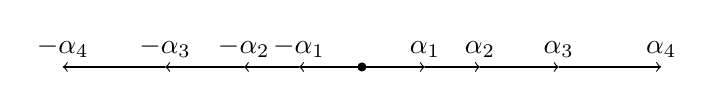
\begin{tikzpicture}
          % center point
          \draw[fill] (0,0) circle (0.05);
          % positive roots
          \draw[->] (0,0) -- (0.8,0) node[above]{$\alpha_1$};
          \draw[->] (0.8,0) -- (1.5,0) node[above]{$\alpha_2$};
          \draw[->] (1.5,0) -- (2.5,0) node[above]{$\alpha_3$};
          \draw[->] (2.5,0) -- (3.8,0) node[above]{$\alpha_4$};
          % negative roots
          \draw[->] (0,0) -- (-0.8,0) node[above]{$-\alpha_1$};
          \draw[->] (-0.8,0) -- (-1.5,0) node[above]{$-\alpha_2$};
          \draw[->] (-1.5,0) -- (-2.5,0) node[above]{$-\alpha_3$};
          \draw[->] (-2.5,0) -- (-3.8,0) node[above]{$-\alpha_4$};
        \end{tikzpicture}
      \end{center}
    \item
      A root system in~$V$ is reduced if and only if it is of the form~$R = \{\alpha, -\alpha\}$ for some nonzero~$\alpha \in V$.
      \begin{center}
        \begin{tikzpicture}
          % center point
          \draw[fill] (0,0) circle (0.05);
          % roots
          \draw[->] (0,0) -- (2,0) node[right]{$\alpha$};
          \draw[->] (0,0) -- (-2,0) node[left]{$-\alpha$};
        \end{tikzpicture}
      \end{center}
    \item
      A root system in~$V$ is crystallographic if and only if it is of the form~$R = \{\alpha, -\alpha\}$ for some nonzero~$\alpha \in V$ or of the form~$R = \{\alpha, 2\alpha, -\alpha, -2\alpha\}$ for some nonzero~$\alpha \in V$.
      \begin{center}
        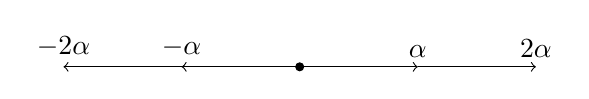
\begin{tikzpicture}
          % center point
          \draw[fill] (0,0) circle (0.05);
          % roots
          \draw[->] (0,0) -- (1.5,0) node[above]{$\alpha$};
          \draw[->] (1.5,0) -- (3,0) node[above]{$2\alpha$};
          \draw[->] (0,0) -- (-1.5,0) node[above]{$-\alpha$};
          \draw[->] (-1.5,0) -- (-3,0) node[above]{$-2\alpha$};
        \end{tikzpicture}
      \end{center}
      
      Indeed, if~$R = \{\alpha, -\alpha\}$ then~$R$ is crystallographic, and if~$R = \{\alpha, -\alpha, 2\alpha, -2\alpha\}$ then we also find that~$s(2\alpha) = 2s(\alpha) \in 2(\alpha + \Integer \alpha) \subseteq 2\alpha + \Integer$.
      
      Suppose now conversely that~$R$ is any crystallographic root system in~$V$.
      Then~$R$ contains some nonzero vector~$\alpha$.
      If~$\beta \in R$ is any other root then~$\beta = \lambda \alpha$ for some nonzero scalar~$\lambda$.
      Then
      \[
        \Integer \alpha
        \ni
        s(\beta) - \beta
        =
        -2 \beta
        =
        -2 \lambda \alpha
      \]
      and thus~$-2 \lambda \in \Integer$, i.e.~$\lambda \in 2^{-1} \Integer$.
      By switching the roles of~$\alpha$ and~$\beta$ we find in the same way that also~$\lambda^{-1} \in 2^{-1} \Integer$.
      We have found that~$\lambda$ is a nonzero half-integer whose inverse~$\lambda^{-1}$ is again a half-integer.
      This leaves for~$\lambda$ only the choices~$\pm 1$,~$\pm 2$ and~$\pm 1/2$, which proves the assertion.
  \end{enumerate}
  
  The above argument shows more generally that if~$R$ is a crystallographic root system in any vector space~$V$, then for every root~$\alpha \in R$ the only multiples of~$R$ that can again be roots are~$\pm \alpha$,~$\pm 2 \alpha$ and~$\pm \alpha/2$.
\end{example}


\begin{examples}[Root system in~$\Real^n$]
  \label{root systems in Rn}
  Suppose that~$V$ is a real vector space with inner product~$\inner{-,-}$.
  Then we denote for every nonzero vector~$\alpha \in V$ by
  \[
    H_\alpha
    \defined
    \{
      v \in V
    \suchthat
      \inner{v,\alpha}
      =
      0
    \}
  \]
  the hyperplane orthogonal to~$\alpha$ and by~$s_\alpha \colon V \to V$ the reflection at~$H_\alpha$, as explained in \cref{recalling reflections}.
  Observe that for~$V = \Real^n$ we have the following special reflections:
  \begin{itemize}
    \item
      The reflection~$s_{e_i}$ is given by~$s_{e_i}(e_i) = -e_i$ and~$s_{e_i}(e_j) = e_j$ for~$j \neq i$.
      This means that this reflection flips the sign of the~{\howmanyth{$i$}} standard basis vector.
    \item
      To calculate the reflection~$s_{e_i - e_j}$ we observe that
      \[
        H_\alpha
        =
        \gen{
          e_i + e_j,
          e_1
          \dotsc,
          \widehat{e_i},
          \dotsc,
          \widehat{e_j},
          \dotsc,
          e_n
        }_{\Real}
      \]
      since this linear subspace is orthogonal to~$e_i - e_j$ and of the right dimension (namely~$n-1$).
      It follows that~$s_{e_i-e_j}(e_k) = e_k$ for~$k \neq i,j$.
      We also find
      \[
        s_{e_i-e_j}(e_i)
        =
        s_{e_i-e_j}\left( \frac{e_i - e_j}{2} + \frac{e_i + e_j}{2} \right)
        =
        -\frac{e_i - e_j}{2} + \frac{e_i + e_j}{2}
        =
        e_j
      \]
      and therefore also~$s_{e_i-e_j}(e_j) = e_i$.
      This shows that the reflection~$s_{e_i-e_j}$ swaps the two standard basis vectors~$e_i+e_j$.
    \item
      The reflections~$s_{e_i}$ is an isometry, and therefore
      \[
        s_{e_i + e_j}
        =
        s_{s_{e_j}(e_i - e_j)}
        =
        s_{e_j} \circ s_{e_i - e_j} \circ s_{e_j}^{-1}
        =
        s_{e_j} \circ s_{e_i - e_j} \circ s_{e_j}
      \]
      as seen in \cref{recalling reflections}.
      We find from the above explicit descriptions of the reflections~$s_{e_i}$ and~$s_{e_i - e_j}$ that the reflection~$s_{e_i + e_j}$ fixes the standard basis vectors~$e_k$ with~$k \neq i,j$ and is given on the other two standard basis vectors by~$s_{e_i + e_j}(e_i) = -e_j$ and~$s_{e_i + e_j}(e_j) = -e_i$.
  \end{itemize}
  
  We now use the above calculations to give examples of root systems~$R$ in (a suitable linear subspace of)~$\Real^n$ for which the reflection~$s_\alpha$ for~$\alpha \in R$ is the orthogonal reflection at the hyperplane~$H_\alpha$ as above.
  This means that
  \[
    s_\alpha(x)
    =
    x - 2 \frac{(x,\alpha)}{\norm{\alpha}^2} \alpha \,,
  \]
  as explained in \cref{recalling reflections}.
  Any such constructed root system~$R$ will therefore be crystallographic if and only if~$2 (\alpha,\beta)/\norm{\alpha}^2 \in \Integer$ for all~$\alpha, \beta \in R$.

  
  \begin{enumerate}
    \item
      The set~$R = \{ \pm e_i \suchthat i = 1, \dotsc, n\}$ is a reduced, crystallographic root system in~$\Real^n$.
      
      The set~$R$ spans~$\Real^n$ and does not contain the zero vector, and the reflections~$s_{\pm e_i} = s_{e_i}$ flip the standard basis vector~$e_i$, so that~$s_{e_i}(R) \subseteq R$.
      This shows that~$R$ is a root system, and we see (directly) that it is reduced.
      It is crystallographic since
      \[
        2 \frac{(e_i, e_j)}{\norm{e_i}^2}
        =
        2 \delta_{ij}
        \in
        \Integer
      \]
      for all~$i, j = 1, \dotsc, n$.
      
      For small values of~$n$ these root systems looks as follows:
      \begin{center}
        \begingroup
        \setlength{\tabcolsep}{18pt} %normal 6pt
        \begin{tabular}{ccc}
          \begin{tikzpicture}
            % center point
            \draw[fill] (0,0) circle (0.05);
            % roots
            \draw[->] (0,0) -- (1,0);
            \draw[->] (0,0) -- (-1,0);
            \draw[opacity=0] (0,0) -- (0,1);
            \draw[opacity=0] (0,0) -- (0,-1);
          \end{tikzpicture}
          &
          \begin{tikzpicture}
            % roots
            \draw[->] (0,0) -- (1,0);
            \draw[->] (0,0) -- (-1,0);
            \draw[->] (0,0) -- (0,1);
            \draw[->] (0,0) -- (0,-1);
          \end{tikzpicture}
          &
          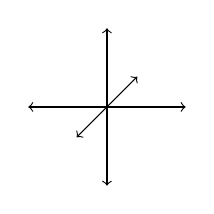
\begin{tikzpicture}
            % roots
            \draw[->] (0,0,0) -- (1,0,0);
            \draw[->] (0,0,0) -- (-1,0,0);
            \draw[->] (0,0,0) -- (0,1,0);
            \draw[->] (0,0,0) -- (0,-1,0);
            \draw[->] (0,0,0) -- (0,0,1);
            \draw[->] (0,0,0) -- (0,0,-1);
%             % cube
%             \draw[dashed] (1,1,1) -- (1,1,-1);
%             \draw[dashed] (1,-1,1) -- (1,-1,-1);
%             \draw[dashed] (-1,1,1) -- (-1,1,-1);
%             \draw[dashed] (-1,-1,1) -- (-1,-1,-1);
%             \draw[dashed] (1,1,1) -- (1,-1,1);
%             \draw[dashed] (1,1,-1) -- (1,-1,-1);
%             \draw[dashed] (-1,1,1) -- (-1,-1,1);
%             \draw[dashed] (-1,1,-1) -- (-1,-1,-1);
%             \draw[dashed] (1,1,1) -- (-1,1,1);
%             \draw[dashed] (1,-1,1) -- (-1,-1,1);
%             \draw[dashed] (1,1,-1) -- (-1,1,-1);
%             \draw[dashed] (1,-1,-1) -- (-1,-1,-1);
          \end{tikzpicture}
          \\
          $n = 1$
          &
          $n = 2$
          &
          $n = 3$
        \end{tabular}
        \endgroup
      \end{center}
    \item
      The set~$R = \{ e_i - e_j \suchthat 1 \leq i \neq j \leq n\} \subseteq \Real^n$ is a reduced, crystallographic root system in
      \[
        V
        =
        \{
          (x_1, \dotsc, x_n) \in \Real^n
        \suchthat
          x_1 + \dotsb + x_n = 0
        \} \,.
      \]
      
      The set~$R$ generates~$V$ as a vector space and it does not contain the zero vector.
      The reflection~$s_{e_i - e_j}$ swaps the standard basis vectors~$e_i$ and~$e_j$, an operation under which~$R$ is invariant.
      Thus~$s_{e_i - e_j}(R) \subseteq R$ for all~$1 \leq i \neq j \leq n$.
      This shows that~$R$ is indeed a root system, and we see (directly) that it is reduced.
      We have
      \[
        2 \frac{(e_i - e_j, e_k - e_l)}{\norm{e_i - e_j}^2}
        =
        2 \frac{\delta_{ik} + \delta_{jl} - \delta_{il} - \delta_{jk} }{2}
        =
        \delta_{ik} + \delta_{jl} - \delta_{il} - \delta_{jk}
        \in
        \Integer
      \]
      for all~$i \neq j$ and~$k \neq l$, whence~$R$ is crystallographic.
      
      For~$n = 2$ the roots are middle points of the cube~$[1,-1]^3$:
      \begin{center}
      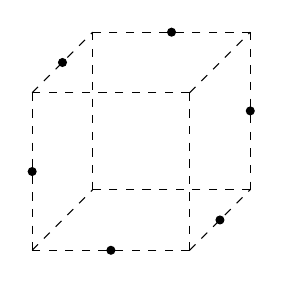
\begin{tikzpicture}
        % roots
        \draw[fill] (1,-1,0) circle (0.05);
        \draw[fill] (-1,1,0) circle (0.05);
        \draw[fill] (1,0,-1) circle (0.05);
        \draw[fill] (-1,0,1) circle (0.05);
        \draw[fill] (0,1,-1) circle (0.05);
        \draw[fill] (0,-1,1) circle (0.05);
        % cube
        \draw[dashed] (1,1,1) -- (1,1,-1);
        \draw[dashed] (1,-1,1) -- (1,-1,-1);
        \draw[dashed] (-1,1,1) -- (-1,1,-1);
        \draw[dashed] (-1,-1,1) -- (-1,-1,-1);
        \draw[dashed] (1,1,1) -- (1,-1,1);
        \draw[dashed] (1,1,-1) -- (1,-1,-1);
        \draw[dashed] (-1,1,1) -- (-1,-1,1);
        \draw[dashed] (-1,1,-1) -- (-1,-1,-1);
        \draw[dashed] (1,1,1) -- (-1,1,1);
        \draw[dashed] (1,-1,1) -- (-1,-1,1);
        \draw[dashed] (1,1,-1) -- (-1,1,-1);
        \draw[dashed] (1,-1,-1) -- (-1,-1,-1);
      \end{tikzpicture}
      \end{center}
      We see that in the subspace~$V$, which is the plane going through these six points, the roots form a regular hexagon:
      \begin{center}
      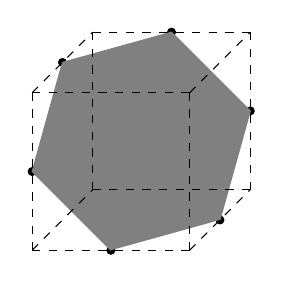
\begin{tikzpicture}
        % roots
        \draw[fill] (1,-1,0) circle (0.05);
        \draw[fill] (-1,1,0) circle (0.05);
        \draw[fill] (1,0,-1) circle (0.05);
        \draw[fill] (-1,0,1) circle (0.05);
        \draw[fill] (0,1,-1) circle (0.05);
        \draw[fill] (0,-1,1) circle (0.05);
        \draw[fill, gray] (1,-1,0) -- (1,0,-1) -- (0,1,-1) -- (-1,1,0) -- (-1,0,1) -- (0,-1,1);
        % cube
        \draw[dashed] (1,1,1) -- (1,1,-1);
        \draw[dashed] (1,-1,1) -- (1,-1,-1);
        \draw[dashed] (-1,1,1) -- (-1,1,-1);
        \draw[dashed] (-1,-1,1) -- (-1,-1,-1);
        \draw[dashed] (1,1,1) -- (1,-1,1);
        \draw[dashed] (1,1,-1) -- (1,-1,-1);
        \draw[dashed] (-1,1,1) -- (-1,-1,1);
        \draw[dashed] (-1,1,-1) -- (-1,-1,-1);
        \draw[dashed] (1,1,1) -- (-1,1,1);
        \draw[dashed] (1,-1,1) -- (-1,-1,1);
        \draw[dashed] (1,1,-1) -- (-1,1,-1);
        \draw[dashed] (1,-1,-1) -- (-1,-1,-1);
      \end{tikzpicture}
      \end{center}
      The root system therefore looks as follows:
      \begin{center}
      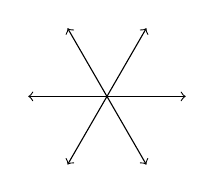
\begin{tikzpicture}
        \foreach \ang in {60, 120, ..., 360}{
          \draw[->] (0,0) -- (\ang:1);
        }
      \end{tikzpicture}
      \end{center}
      For~$n = 4$ the root system (which lives inside the {\fourdimensional} space~$\Real^4$) looks inside of its span~$V$ (which is {\threedimensional} as follows:
      \begin{center}
      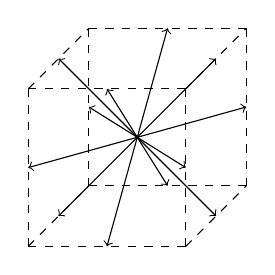
\begin{tikzpicture}
        % long roots
        \draw[->] (0,0,0) -- (1,1,0);
        \draw[->] (0,0,0) -- (1,-1,0);
        \draw[->] (0,0,0) -- (-1,1,0);
        \draw[->] (0,0,0) -- (-1,-1,0);
        \draw[->] (0,0,0) -- (1,0,1);
        \draw[->] (0,0,0) -- (1,0,-1);
        \draw[->] (0,0,0) -- (-1,0,1);
        \draw[->] (0,0,0) -- (-1,0,-1);
        \draw[->] (0,0,0) -- (0,1,1);
        \draw[->] (0,0,0) -- (0,1,-1);
        \draw[->] (0,0,0) -- (0,-1,1);
        \draw[->] (0,0,0) -- (0,-1,-1);
        % cube
        \draw[dashed] (1,1,1) -- (1,1,-1);
        \draw[dashed] (1,-1,1) -- (1,-1,-1);
        \draw[dashed] (-1,1,1) -- (-1,1,-1);
        \draw[dashed] (-1,-1,1) -- (-1,-1,-1);
        \draw[dashed] (1,1,1) -- (1,-1,1);
        \draw[dashed] (1,1,-1) -- (1,-1,-1);
        \draw[dashed] (-1,1,1) -- (-1,-1,1);
        \draw[dashed] (-1,1,-1) -- (-1,-1,-1);
        \draw[dashed] (1,1,1) -- (-1,1,1);
        \draw[dashed] (1,-1,1) -- (-1,-1,1);
        \draw[dashed] (1,1,-1) -- (-1,1,-1);
        \draw[dashed] (1,-1,-1) -- (-1,-1,-1);
      \end{tikzpicture}
      \end{center}
      The roots~$\pm e_i \pm e_j$ are the middle points of the edges of the ambient cube~$[-1,1]^3$.
      \begin{center}
      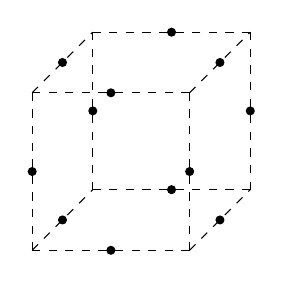
\begin{tikzpicture}
        % roots
        \draw[fill] (1,1,0) circle (0.05);
        \draw[fill] (1,-1,0) circle (0.05);
        \draw[fill] (-1,1,0) circle (0.05);
        \draw[fill] (-1,-1,0) circle (0.05);
        \draw[fill] (1,0,1) circle (0.05);
        \draw[fill] (1,0,-1) circle (0.05);
        \draw[fill] (-1,0,1) circle (0.05);
        \draw[fill] (-1,0,-1) circle (0.05);
        \draw[fill] (0,1,1) circle (0.05);
        \draw[fill] (0,1,-1) circle (0.05);
        \draw[fill] (0,-1,1) circle (0.05);
        \draw[fill] (0,-1,-1) circle (0.05);
        % cube
        \draw[dashed] (1,1,1) -- (1,1,-1);
        \draw[dashed] (1,-1,1) -- (1,-1,-1);
        \draw[dashed] (-1,1,1) -- (-1,1,-1);
        \draw[dashed] (-1,-1,1) -- (-1,-1,-1);
        \draw[dashed] (1,1,1) -- (1,-1,1);
        \draw[dashed] (1,1,-1) -- (1,-1,-1);
        \draw[dashed] (-1,1,1) -- (-1,-1,1);
        \draw[dashed] (-1,1,-1) -- (-1,-1,-1);
        \draw[dashed] (1,1,1) -- (-1,1,1);
        \draw[dashed] (1,-1,1) -- (-1,-1,1);
        \draw[dashed] (1,1,-1) -- (-1,1,-1);
        \draw[dashed] (1,-1,-1) -- (-1,-1,-1);
      \end{tikzpicture}
      \end{center}
      
    \item
      The set~$R = \{ \pm e_i \pm e_j \suchthat 1 \leq i \neq j \leq n \}$ is a reduced, crystallographic root system in~$\Real^n$ for~$n \geq 2$.
      
      The vector space~$\Real^n$ is spanned by~$R$ since~$e_i = (e_i - e_j)/2 + (e_i + e_j)/2$ for any~$j \neq i$.
      The reflection~$s_{e_i - e_j}$ swaps the two standard basis vectors~$e_i$ and~$e_j$, an operation under which~$R$ is closed.
      The reflection~$s_{e_i + e_j}$ again swaps the two standard basis vectors~$e_i$ and~$e_j$ but then also flips their signs.
      But this is again an operation under which~$R$ is closed.
      We thus find that~$R$ is indeed a root system.
      We see (directly) that it is reduced.
      We have for all~$1 \leq i \neq j \leq n$ and~$1 \leq k \neq l \leq n$ that
      \[
        2 \frac{(e_i \pm e_j, e_k \pm e_l)}{\norm{e_i \pm e_j}^2}
        =
        2 \frac{\delta_{ik} + \delta_{jl} \pm \delta_{il} \pm \delta_{jk}}{2}
        =
        \delta_{ik} + \delta_{jl} \pm \delta_{il} \pm \delta_{jk}
        \in
        \Integer \,,
      \]
      which shows that~$R$ is crystallographic.
      
      For small values of~$n$ these root systems look as follows:
      \begin{center}
        \begingroup
        \setlength{\tabcolsep}{24pt} %normal 6pt
        \begin{tabular}{cc}
          
\begin{tikzpicture}
            % roots
            \draw[->] (0,0) -- (1,1);
            \draw[->] (0,0) -- (1,-1);
            \draw[->] (0,0) -- (-1,1);
            \draw[->] (0,0) -- (-1,-1);
          \end{tikzpicture}
          &
          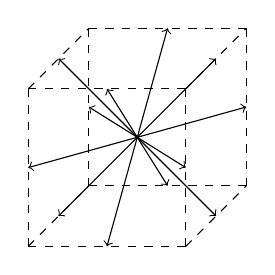
\begin{tikzpicture}
            % roots
            \draw[->] (0,0,0) -- (1,1,0);
            \draw[->] (0,0,0) -- (1,-1,0);
            \draw[->] (0,0,0) -- (-1,1,0);
            \draw[->] (0,0,0) -- (-1,-1,0);
            \draw[->] (0,0,0) -- (1,0,1);
            \draw[->] (0,0,0) -- (1,0,-1);
            \draw[->] (0,0,0) -- (-1,0,1);
            \draw[->] (0,0,0) -- (-1,0,-1);
            \draw[->] (0,0,0) -- (0,1,1);
            \draw[->] (0,0,0) -- (0,1,-1);
            \draw[->] (0,0,0) -- (0,-1,1);
            \draw[->] (0,0,0) -- (0,-1,-1);
            % cube
            \draw[dashed] (1,1,1) -- (1,1,-1);
            \draw[dashed] (1,-1,1) -- (1,-1,-1);
            \draw[dashed] (-1,1,1) -- (-1,1,-1);
            \draw[dashed] (-1,-1,1) -- (-1,-1,-1);
            \draw[dashed] (1,1,1) -- (1,-1,1);
            \draw[dashed] (1,1,-1) -- (1,-1,-1);
            \draw[dashed] (-1,1,1) -- (-1,-1,1);
            \draw[dashed] (-1,1,-1) -- (-1,-1,-1);
            \draw[dashed] (1,1,1) -- (-1,1,1);
            \draw[dashed] (1,-1,1) -- (-1,-1,1);
            \draw[dashed] (1,1,-1) -- (-1,1,-1);
            \draw[dashed] (1,-1,-1) -- (-1,-1,-1);
          \end{tikzpicture}
          \\
          $n = 2$
          &
          $n = 3$
        \end{tabular}
        \endgroup
      \end{center}
      In the case~$n = 3$ the roots~$\pm e_i \pm e_j$ are the middle points of the edges of the ambient cube~$[-1,1]^3$.
      \begin{center}
      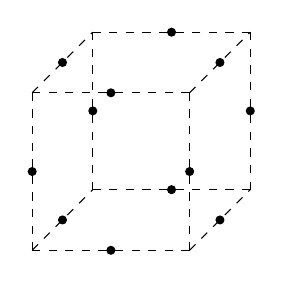
\begin{tikzpicture}
        % roots
        \draw[fill] (1,1,0) circle (0.05);
        \draw[fill] (1,-1,0) circle (0.05);
        \draw[fill] (-1,1,0) circle (0.05);
        \draw[fill] (-1,-1,0) circle (0.05);
        \draw[fill] (1,0,1) circle (0.05);
        \draw[fill] (1,0,-1) circle (0.05);
        \draw[fill] (-1,0,1) circle (0.05);
        \draw[fill] (-1,0,-1) circle (0.05);
        \draw[fill] (0,1,1) circle (0.05);
        \draw[fill] (0,1,-1) circle (0.05);
        \draw[fill] (0,-1,1) circle (0.05);
        \draw[fill] (0,-1,-1) circle (0.05);
        % cube
        \draw[dashed] (1,1,1) -- (1,1,-1);
        \draw[dashed] (1,-1,1) -- (1,-1,-1);
        \draw[dashed] (-1,1,1) -- (-1,1,-1);
        \draw[dashed] (-1,-1,1) -- (-1,-1,-1);
        \draw[dashed] (1,1,1) -- (1,-1,1);
        \draw[dashed] (1,1,-1) -- (1,-1,-1);
        \draw[dashed] (-1,1,1) -- (-1,-1,1);
        \draw[dashed] (-1,1,-1) -- (-1,-1,-1);
        \draw[dashed] (1,1,1) -- (-1,1,1);
        \draw[dashed] (1,-1,1) -- (-1,-1,1);
        \draw[dashed] (1,1,-1) -- (-1,1,-1);
        \draw[dashed] (1,-1,-1) -- (-1,-1,-1);
      \end{tikzpicture}
      \end{center}
    \item
      The set~$R = \{ \pm e_i \suchthat i = 1, \dotsc, n \} \cup \{ \pm e_i \pm e_j \suchthat 1 \leq i \neq j \leq n\}$ is a reduced, crystallographic root system in~$\Real^n$.
      
      The set~$R$ spans~$\Real^n$ it contains the standard basis.
      The reflection~$s_{e_i}$ swaps the sign of the standard basis vector~$e_i$, an operation under which~$R$ is invariant.
      The reflections~$s_{e_i - e_j}$ and~$s_{e_i + e_j}$ fix the standard basis vectors~$e_k$ with~$k \neq i,j$ and swap the standard basis vectors~$e_i$ and~$e_j$, while~$s_{e_i+e_j}$ then also flips the sign of~$e_i$ and~$e_j$.
      The set~$R$ is also invariant under these operations.
      This shows that~$R$ is indeed a root system and we see (directly) that it is reduced.
      
      To see that~$R$ is crystallographic we can reuse the calculations from the previous examples.
      It then remains to check that~$2 (\alpha, \beta)/\norm{\alpha}^2 \in \Integer$ for the cases~$\alpha = e_i$ and~$\beta = e_j \pm e_k$ with~$j \neq k$, and~$\beta = e_i \pm e_j$ and~$\alpha = e_k$ for~$i,j \neq k$.
      In the first case we have
      \[
        2 \frac{(e_i, e_j - e_k)}{\norm{e_i}^2}
        =
        2 \frac{\delta_{ij} - \delta_{ik}}{1}
        =
        2 \delta_{ij} - 2 \delta_{ik}
        \in
        \Integer
      \]
      and in the second case we have similarly
      \[
        2 \frac{(e_i - e_j, e_k)}{\norm{e_i - e_j}^2}
        =
        2 \frac{\delta_{ik} - \delta_{jk}}{2}
        =
        \delta_{ik} - \delta_{jk}
        \in
        \Integer \,.
      \]
      Thus~$R$ is crystallographic.
      
      For small values of~$n$ these root systems looks as follows:
      \begin{center}
      \begingroup
      \setlength{\tabcolsep}{18pt} %normal 6pt
      \begin{tabular}{ccc}
        \begin{tikzpicture}
          % center point
          \draw[fill] (0,0) circle (0.05);
          % roots
          \draw[->] (0,0) -- (1,0);
          \draw[->] (0,0) -- (-1,0);
          \draw[opacity=0] (0,0) -- (0,1);
          \draw[opacity=0] (0,0) -- (0,-1);
        \end{tikzpicture}
        &
        
\begin{tikzpicture}
          % short roots
          \draw[->] (0,0) -- (1,0);
          \draw[->] (0,0) -- (-1,0);
          \draw[->] (0,0) -- (0,1);
          \draw[->] (0,0) -- (0,-1);
          % long rots
          \draw[->] (0,0) -- (1,1);
          \draw[->] (0,0) -- (1,-1);
          \draw[->] (0,0) -- (-1,1);
          \draw[->] (0,0) -- (-1,-1);
        \end{tikzpicture}
        &
        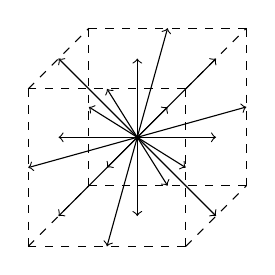
\begin{tikzpicture}
          % short roots
          \draw[->] (0,0,0) -- (1,0,0);
          \draw[->] (0,0,0) -- (-1,0,0);
          \draw[->] (0,0,0) -- (0,1,0);
          \draw[->] (0,0,0) -- (0,-1,0);
          \draw[->] (0,0,0) -- (0,0,1);
          \draw[->] (0,0,0) -- (0,0,-1);
          % long roots
          \draw[->] (0,0,0) -- (1,1,0);
          \draw[->] (0,0,0) -- (1,-1,0);
          \draw[->] (0,0,0) -- (-1,1,0);
          \draw[->] (0,0,0) -- (-1,-1,0);
          \draw[->] (0,0,0) -- (1,0,1);
          \draw[->] (0,0,0) -- (1,0,-1);
          \draw[->] (0,0,0) -- (-1,0,1);
          \draw[->] (0,0,0) -- (-1,0,-1);
          \draw[->] (0,0,0) -- (0,1,1);
          \draw[->] (0,0,0) -- (0,1,-1);
          \draw[->] (0,0,0) -- (0,-1,1);
          \draw[->] (0,0,0) -- (0,-1,-1);
          % cube
          \draw[dashed] (1,1,1) -- (1,1,-1);
          \draw[dashed] (1,-1,1) -- (1,-1,-1);
          \draw[dashed] (-1,1,1) -- (-1,1,-1);
          \draw[dashed] (-1,-1,1) -- (-1,-1,-1);
          \draw[dashed] (1,1,1) -- (1,-1,1);
          \draw[dashed] (1,1,-1) -- (1,-1,-1);
          \draw[dashed] (-1,1,1) -- (-1,-1,1);
          \draw[dashed] (-1,1,-1) -- (-1,-1,-1);
          \draw[dashed] (1,1,1) -- (-1,1,1);
          \draw[dashed] (1,-1,1) -- (-1,-1,1);
          \draw[dashed] (1,1,-1) -- (-1,1,-1);
          \draw[dashed] (1,-1,-1) -- (-1,-1,-1);
        \end{tikzpicture}
        \\
        $n = 1$
        &
        $n = 2$
        &
        $n = 3$
      \end{tabular}
      \endgroup
      \end{center}
      In the case~$n = 3$ the root system consists of the centers of the faces of the cube~$[-1,1]^3$ (these are the roots~$\pm e_i$) together with the middle points of the edges of the cube (these are the roots~$\pm e_i \pm e_j$).
      \begin{center}
        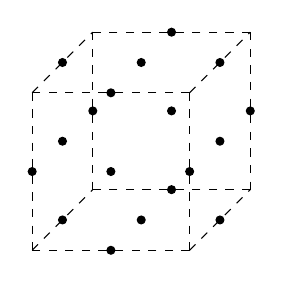
\begin{tikzpicture}
          % short roots
          \draw[fill] (1,0,0) circle (0.05);
          \draw[fill] (-1,0,0) circle (0.05);
          \draw[fill] (0,1,0) circle (0.05);
          \draw[fill] (0,-1,0) circle (0.05);
          \draw[fill] (0,0,1) circle (0.05);
          \draw[fill] (0,0,-1) circle (0.05);
          % long roots
          \draw[fill] (1,1,0) circle (0.05);
          \draw[fill] (1,-1,0) circle (0.05);
          \draw[fill] (-1,1,0) circle (0.05);
          \draw[fill] (-1,-1,0) circle (0.05);
          \draw[fill] (1,0,1) circle (0.05);
          \draw[fill] (1,0,-1) circle (0.05);
          \draw[fill] (-1,0,1) circle (0.05);
          \draw[fill] (-1,0,-1) circle (0.05);
          \draw[fill] (0,1,1) circle (0.05);
          \draw[fill] (0,1,-1) circle (0.05);
          \draw[fill] (0,-1,1) circle (0.05);
          \draw[fill] (0,-1,-1) circle (0.05);
          % cube
          \draw[dashed] (1,1,1) -- (1,1,-1);
          \draw[dashed] (1,-1,1) -- (1,-1,-1);
          \draw[dashed] (-1,1,1) -- (-1,1,-1);
          \draw[dashed] (-1,-1,1) -- (-1,-1,-1);
          \draw[dashed] (1,1,1) -- (1,-1,1);
          \draw[dashed] (1,1,-1) -- (1,-1,-1);
          \draw[dashed] (-1,1,1) -- (-1,-1,1);
          \draw[dashed] (-1,1,-1) -- (-1,-1,-1);
          \draw[dashed] (1,1,1) -- (-1,1,1);
          \draw[dashed] (1,-1,1) -- (-1,-1,1);
          \draw[dashed] (1,1,-1) -- (-1,1,-1);
          \draw[dashed] (1,-1,-1) -- (-1,-1,-1);
        \end{tikzpicture}
        \end{center}
    \item
      The set~$R = \{ \pm 2 e_i \suchthat i = 1, \dotsc, n \} \cup \{ \pm e_i \pm e_j \suchthat 1 \leq i \neq j \leq n\}$ is a reduced, crystallographic root system in~$\Real^n$.
      That~$R$ is a reduced root system can be seen in the same way as in the previous example.
      To see that~$R$ is crystallographic we calculate as in the previous case that
      \begin{gather*}
        2 \frac{(2e_i, e_j - e_k)}{\norm{2 e_i}^2}
        =
        2 \frac{2\delta_{ij} - 2\delta_{ik}}{4}
        =
        \delta_{ij} - 2 \delta_{ik}
        \in
        \Integer
      \shortintertext{and}
        2 \frac{(e_i - e_j, 2 e_k)}{\norm{e_i - e_j}^2}
        =
        2 \frac{2 \delta_{ik} - 2 \delta_{jk}}{2}
        =
        4 \delta_{ik} - \delta_{jk}
        \in
        \Integer \,.
      \end{gather*}
      
      For small values of~$n$ these root systems looks as follows:
      \begin{center}
      \begingroup
      \setlength{\tabcolsep}{12pt} %normal 6pt
      \begin{tabular}{ccc}
        \begin{tikzpicture}[scale=0.7]
          % center point
          \draw[fill] (0,0) circle (0.05);
          % roots
          \draw[->] (0,0) -- (2,0);
          \draw[->] (0,0) -- (-2,0);
          \draw[opacity=0] (0,0) -- (0,2);
          \draw[opacity=0] (0,0) -- (0,-2);
        \end{tikzpicture}
        &
        \begin{tikzpicture}[scale=0.7]
          % short roots
          \draw[->] (0,0) -- (2,0);
          \draw[->] (0,0) -- (-2,0);
          \draw[->] (0,0) -- (0,2);
          \draw[->] (0,0) -- (0,-2);
          % long rots
          \draw[->] (0,0) -- (1,1);
          \draw[->] (0,0) -- (1,-1);
          \draw[->] (0,0) -- (-1,1);
          \draw[->] (0,0) -- (-1,-1);
        \end{tikzpicture}
        &
        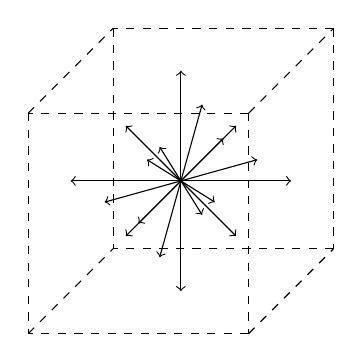
\begin{tikzpicture}[scale=0.7]
          % short roots
          \draw[->] (0,0,0) -- (2,0,0);
          \draw[->] (0,0,0) -- (-2,0,0);
          \draw[->] (0,0,0) -- (0,2,0);
          \draw[->] (0,0,0) -- (0,-2,0);
          \draw[->] (0,0,0) -- (0,0,2);
          \draw[->] (0,0,0) -- (0,0,-2);
          % long roots
          \draw[->] (0,0,0) -- (1,1,0);
          \draw[->] (0,0,0) -- (1,-1,0);
          \draw[->] (0,0,0) -- (-1,1,0);
          \draw[->] (0,0,0) -- (-1,-1,0);
          \draw[->] (0,0,0) -- (1,0,1);
          \draw[->] (0,0,0) -- (1,0,-1);
          \draw[->] (0,0,0) -- (-1,0,1);
          \draw[->] (0,0,0) -- (-1,0,-1);
          \draw[->] (0,0,0) -- (0,1,1);
          \draw[->] (0,0,0) -- (0,1,-1);
          \draw[->] (0,0,0) -- (0,-1,1);
          \draw[->] (0,0,0) -- (0,-1,-1);
          % cube
          \draw[dashed] (2,2,2) -- (2,2,-2);
          \draw[dashed] (2,-2,2) -- (2,-2,-2);
          \draw[dashed] (-2,2,2) -- (-2,2,-2);
          \draw[dashed] (-2,-2,2) -- (-2,-2,-2);
          \draw[dashed] (2,2,2) -- (2,-2,2);
          \draw[dashed] (2,2,-2) -- (2,-2,-2);
          \draw[dashed] (-2,2,2) -- (-2,-2,2);
          \draw[dashed] (-2,2,-2) -- (-2,-2,-2);
          \draw[dashed] (2,2,2) -- (-2,2,2);
          \draw[dashed] (2,-2,2) -- (-2,-2,2);
          \draw[dashed] (2,2,-2) -- (-2,2,-2);
          \draw[dashed] (2,-2,-2) -- (-2,-2,-2);
        \end{tikzpicture}
        \\
        $n = 1$
        &
        $n = 2$
        &
        $n = 3$
      \end{tabular}
      \endgroup
      \end{center}
    \item
      Let~$n \geq 1$ and let~$R$ be the subset of~$\Real^2$ given by
      \[
        R
        =
        \left\{
          \left(
            \cos\left( k \cdot \frac{\pi}{n} \right),
            \sin\left( k \cdot \frac{\pi}{n} \right) 
          \right)
        \suchthat*
          k = 0, \dotsc, 2n-1
        \right\}
      \]
      This means that~$R$ consists of the vertices of a regular~{\gon{$2n$}}, and for small~$n$ we can visualize~$R$ as follows:
      \[
        \begingroup
        \renewcommand{\arraystretch}{1.5}
        \begin{array}{cccc}
          \vcenter{
          \hbox{
          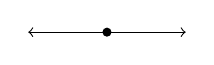
\begin{tikzpicture}
            \draw[->] (0,0) -- (1,0);
            \draw[->] (0,0) -- (-1,0);
            \draw[fill] (0,0) circle (0.05);
          \end{tikzpicture}
          }
          }
          &
          \vcenter{
          \hbox{
          \begin{tikzpicture}
            \foreach \ang in {90, 180, 270, 360}{
              \draw[->] (0,0) -- (\ang:1);
%              \draw[fill] (\ang:1) circle (0.05);
%              \draw (\ang:1) -- (\ang+90:1);
            }
          \end{tikzpicture}
          }
          }
          &
          \vcenter{
          \hbox{
          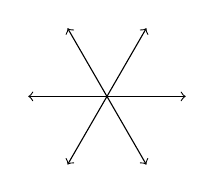
\begin{tikzpicture}
            \foreach \ang in {60, 120, ..., 360}{
              \draw[->] (0,0) -- (\ang:1);
%              \draw (\ang:1) -- (\ang+60:1);
            }
          \end{tikzpicture}
          }
          }
          &
          \vcenter{
          \hbox{
          
\begin{tikzpicture}
            \foreach \ang in {45, 90, ..., 360}{
              \draw[->] (0,0) -- (\ang:1);
%              \draw (\ang:1) -- (\ang+45:1);
            }
          \end{tikzpicture}
          }
          }
          \\
          n = 1
          &
          n = 2
          &
          n = 3
          &
          n = 4
        \end{array}
        \endgroup
      \]
      We see (directly) that~$R$ is always a reduced root system.
      For~$n = 1, 2, 3$ we have already encountered these root systems above, and have seen that they are crystallographic.
      But for~$n \geq 4$ this is not the case:
      Let~$\alpha, \beta \in R$ and let~$\theta$ be the unoriented angle between~$\alpha$ and~$\beta$, i.e.~$\beta \in [0,\pi]$.Then
      \[
        2 \frac{(\alpha, \beta)}{\norm{\alpha}^2}
        =
        2 (\alpha, \beta)
        =
        2 \cos(\theta) \norm{\alpha} \norm{\beta}
        =
        2 \cos(\theta)
      \]
      because~$\norm{\alpha} = \norm{\beta}$.
      For~$R$ to be crystallographic we need~$2 \cos(\theta) \in \Integer$ and thus
      \begin{gather*}
        \cos(\theta)
        \in
        \left\{
          0,
          \pm \frac{1}{2},
          \pm 1
        \right\} \,,
      \shortintertext{which means that}
        \theta
        \in
        \left\{
          \frac{\pi}{2},
          \frac{\pi}{3},
          \frac{2\pi}{3},
          0,
          \pi
        \right\} \,.
      \end{gather*}
      But for~$n \geq 4$ there exist two roots in~$R$ for which the angle between them is smaller or equal to~$\pi/4$.
      (One can take two neighbouring vertices of the regular~{\gon{$n$}} to get the angle~$\pi/n$.)
    \item
      Let~$R$ be the subset of~$\Real^2$ given by
      \begin{align*}
        R
        ={}&
        \left\{
          \left(
            \cos\left( k \cdot \frac{\pi}{3} \right),
            \sin\left( k \cdot \frac{\pi}{3} \right) 
          \right)
        \suchthat*
          k = 0, \dotsc, 5
        \right\}
        \\
        {}&
        \cup
        \left\{
          \sqrt{3}
          \left(
            \cos\left( k \cdot \frac{\pi}{3} + \frac{\pi}{6} \right),
            \sin\left( k \cdot \frac{\pi}{3} + \frac{\pi}{6} \right) 
          \right)
        \suchthat*
          k = 0, \dotsc, 5
        \right\}
      \end{align*}
      The following picture is probably more instructive:
      \begin{center}
      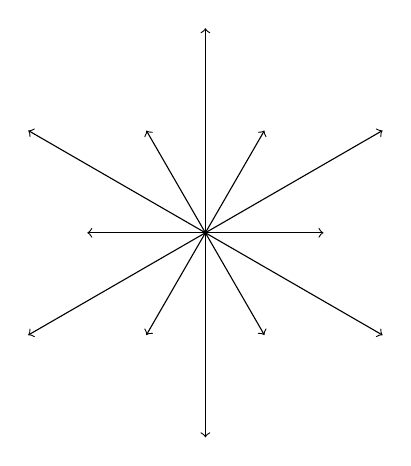
\begin{tikzpicture}[scale = 1.5]
        \foreach \ang in {60, 120, ..., 360}{
          \draw[->] (0,0) -- (\ang:1);
          \draw[->] (0,0) -- (\ang + 30 : 1.732);
        }
      \end{tikzpicture}
      \end{center}
      We see that~$\Real^2$ is spanned by~$R$ and that for every~$\alpha \in R$ the set~$R$ is invariant under the reflection~$s_\alpha$.
      Hence~$R$ is a root system.
      We also see that (directly)~$R$ is reduced.
      By looking long enough at the above picture we also see that~$s_\alpha(\beta) \in \beta + \Integer \alpha$ for all~$\alpha, \beta \in R$, i.e.\ that~$R$ is crystallographic.
  \end{enumerate}
\end{examples}


\begin{examples}
  Some of the examples from \cref{root systems in Rn} can be generalized to general~{\vectorspaces{$\kf$}}:
  \begin{enumerate}
    \item
      We denote for every~$n \geq 1$ by~$\rootA_n$ the root system of rank~$n$ in the vector space
      \begin{align*}
        V
        =
        \{
          (x_1, \dotsc, x_{n+1})
          \in
          \kf^{n+1}
        \suchthat
          x_1 + \dotsb + x_n = 0
        \}
      \shortintertext{that is given by}
        \rootA_n
        =
        \{
          e_i - e_j
        \suchthat
          1 \leq i \neq j \leq n+1
        \} \,.
      \end{align*}
      For all~$1 \leq i \neq j \leq n$ the reflection~$s_{e_i-e_j} \colon V \to V$ is the restriction of the reflection~$\kf^{n+1} \to \kf^{n+1}$ that swaps the standard basis vectors~$e_i$ and~$e_j$ and fixes pointwise all other standard basis vectors.
    \item
      We denote for every~$n \geq 2$ by~$\rootB_n$ the root system of rank~$n$ in the vector space~$\kf^n$ that is given by
      \[
        \rootB_n
        \defined
        \{
          \pm e_i
        \suchthat
          i = 1, \dotsc, n
        \}
        \cup
        \{
          \pm e_i \pm e_j
        \suchthat
          1 \leq i \neq j \leq n
        \} \,.
      \]
      The reflections~$s_{e_i}$ are given by flipping the sign of the standard basis vector~$e_i$, the reflections~$s_{e_i - e_j}$ are given as above by swapping the standard basis vectors~$e_i$ and~$e_j$, and the reflections~$s_{e_i + e_j}$ are given by both swapping the standard basis vectors~$e_i$ and~$e_j$ while also flipping their signs.
    \item
      We denote for every~$n \geq 2$ by~$\rootC_n$ the root system of rank~$n$ in the vector space~$\kf^n$ that is given by
      \[
        \rootC_n
        \defined
        \{
          \pm 2 e_i
        \suchthat
          i = 1, \dotsc, n
        \}
        \cup
        \{
          \pm e_i \pm e_j
        \suchthat
          1 \leq i \neq j \leq n
        \} \,.
      \]
      The reflections associated to~$\rootC_n$ are the same as for~$\rootB_n$, with~$s_{2e_i} = s_{e_i}$.
    \item
      We denote for every~$n \geq 2$ by~$\rootD_n$ the root system of rank~$n$ in the vector space~$\kf^n$ that is given by
      \[
        \rootD_n
        \defined
        \{
          \pm e_i \pm e_j
        \suchthat
          1 \leq i \neq j \leq n
        \} \,.
      \]
      The reflections~$s_{e_i - e_j}$ are as described above.
  \end{enumerate}
\end{examples}


\begin{remark}
  \label{standard root systems have isometric reflections}
  Let~$\inner{-,-}$ be the standard symmetric bilinear form on~$\kf^n$, i.e.~$\inner{x,y} = \sum_{i=1}^n x_i y_i$.
  Then for the root systems~$\rootB_n$,~$\rootC_n$ and~$\rootD_n$ the reflections~$s_\alpha$, where~$\alpha$ is some root, are isometries for~$\inner{-,-}$:
  The standard basis~$e_1, \dotsc, e_n$ of~$\kf^n$ is an orthonormal basis of~$\kf^n$ whence~$s_\alpha$ is an isometry if and only if its representing matrix with respect to this basis is orthogonal.
  This can be seen in (at least) two ways:
  \begin{itemize}
    \item
      Using the above explicit descriptions of these reflections we can write down these matrices and check the assertion by hand.
    \item
      We see from the above explicit description of these reflections that their representing matrices with respect to the standard basis have integer entries (namely~$0$ and~$\pm 1$).
      The claim does therefore not depend on the choice of ground field~$\kf$.
      But we have seen in \cref{root systems in Rn} that the assertion holds for~$\kf = \Real$ (where the standard symmetric form becomes the standard inner product).
      Hence it holds for general~$\kf$.
  \end{itemize}
  
  The reflections~$s_\alpha$ for~$\alpha \in \rootA_n$ are restrictions of reflections~$s'_\alpha$ of~$\kf^n$, which can be shown to be isometries with respect to~$\inner{-,-}$ in the same way as above.
  It follows that~$s_\alpha$ is an isometry with respect to the restriction of~$\inner{-,-}$ to the subspace in which~$\rootA_n$ is a root system.
\end{remark}






\subsection{The Weyl Group}


\begin{definition}
  The \defemph{Weyl~group}\index{Weyl group} of a root system~$R$ in a~{\vectorspace{$\kf$}}~$V$ is the subgroup~$\Weyl(R)$ of~$\GL(V)$ generated by all reflections~$s_\alpha$ with~$\alpha \in R$.
\end{definition}


\begin{remark}
  Let~$R$ be a root system in a~{\vectorspace{$\kf$}}~$V$.
  Every group element~$w \in \Weyl(R)$ leaves the set~$R$ invariant because this holds for the generators~$s_\alpha$ with~$\alpha \in R$.
  The Weyl group~$\Weyl(R)$ therefore acts on the root system~$R$ by restriction of the action on~$V$.
  Every element~$w \in W$ is furthermore uniquely determined by the restriction~$\restrict{w}{R}$ because the set~$R$ spans the vector space~$V$.
  The action of~$\Weyl(R)$ on~$R$ is therefore faithful whence we can identify the Weyl~group~$\Weyl(R)$ with a subgroup of the symmetric group on~$R$.
  We see in particular that the Weyl~group~$\Weyl(R)$ is finite because~$R$ is finite.
\end{remark}


\begin{examples}
  Let us calculate the Weyl~groups of some root systems.
  \begin{enumerate}
    \item
      The only root system in the zero vector space~$0$ is the empty root system~$R = \emptyset$.
      Its Weyl~group is generated by the empty set and is thus the trivial group.
    \item
      The only reflection in a {\onedimensional} vector space~$V$ is the inversion map~$s \colon V \to V$ given by~$x \mapsto -x$.
      Any root system~$R$ in~$V$ is nonempty since it spans~$V$. 
      The Weyl~group~$\Weyl(R)$ does therefore admit nontrivial generators, all of which are necessarily the reflection~$s$.
      This shows that~$\Weyl(R) = \gen{s} \cong \Integer/2$.
    \item
      For our first interesting example we consider the root system~$\rootA_n = \{ e_i - e_j \suchthat 1 \leq i \neq j \leq n+1 \}$ in the~{\vectorspace{$\kf$}}~$V = \{ (x_1, \dotsc, x_{n+1}) \in \kf^{n+1} \suchthat x_1 + \dotsb + x_{n+1} = 0 \}$.
      We will show that its Weyl~group is (isomorphic to) the symmetric group~$\symm_{n+1}$.
      We will construct an isomorphism under which the reflection~$s_{e_i - e_j}$ corresponds to the transposition~$(i,j)$.
      
      The reflection~$s_{e_i - e_j} \colon V \to V$ is the restriction of the reflection~$s'_{e_i - e_j} \colon \kf^{n+1} \to \kf^{n+1}$ that swaps the standard basis vectors~$e_i$ and~$e_j$ and fixes all the other standard basis vectors.
      The subgroup~$W'$ of~$\GL(\kf^{n+1})$ that is generated by the reflections~$s'_\alpha$ with~$\alpha \in \rootA_n$ is the symmetric group~$\symm_{n+1}$, so that the reflecton~$s'_{e_i - e_j}$ corresponds to the transposition~$(i,j)$.
      
      We have a surjective group homomorphism~$r \colon W' \to \Weyl(\rootA_n)$ given by~$w \mapsto \restrict{w}{V}$ because the generator~$s'_\alpha$ of~$W$ restrict to the generator~$s_\alpha$ of~$\Weyl(\rootA_n)$.
      We claim that~$r$ is injective, and thus a group isomorphism.
      This then establishes an isomorphism~$\Weyl(\rootA_n) \cong W' \cong \symm_{n+1}$ under which the reflection~$s_{e_i - e_j}$ corresponds to the transposition~$(i,j)$.
      
      That the group homomorphism~$r \colon W' \to \Weyl(\rootA_n)$ is injective means precisely that~$V$ is faithful as an~{\representation{$\symm_{n+1}$}}, where~$\symm_{n+1}$ acts by permutation of the standard basis vectors.
      To show this faithfulness we consider the decomposition~$\kf^{n+1} = V \oplus L$ with~$L = \gen{(1, \dotsc, 1)}_{\kf}$.
      The permutation action of~$\symm_{n+1}$ on~$\kf^{n+1}$ is faithful and trivial on the subrepresentation~$L$.
      Hence the action of~$\symm_{n+1}$ on the direct summand~$V$ needs to be faithful.
    \item
      Let us now consider the root system~$\rootB_n = \{ \pm e_i \suchthat i = 1, \dotsc, n \} \cup \{ \pm e_i \pm e_j \suchthat 1 \leq i \neq j \leq n \}$ in the vector space~$V = \kf^n$.
      
      The reflection~$s_{e_i}$ flips the sign of the standard basis vector~$e_i$ and fixes all other standard basis vectors.
      The reflection~$s_{e_i - e_j}$ swaps the two standard basis vectors~$e_i$ and~$e_j$ and fixes all other standard basis vectors.
      The reflection~$s_{e_i + e_j}$ swaps the two standard basis vectors~$e_i$ and~$e_j$ and also swappes their signs, and fixes all other standard basis vectors.
      
      We see from these explicit descriptions of the reflections~$s_\alpha$ with~$\alpha \in R$ that these reflections are with respect to the standard basis of~$\kf^n$ given by signed permutation matrices.%
      \footnote{A \defemph{signed permutation matrix}\index{signed permutation matrix} is a matrix that admits in every column and every row precisely one nonzero entry, that is allowed to take on the values~$1$ and~$-1$.
      A signed permutation matrix does therefore have the same form as a permutation matrix, but the occuring nonzero entries need not be~$1$ but are also allowed to be~$-1$.}
      Let us for now identify the group~$\GL(\kf^n)$ with the matrix group~$\GL_n(\kf)$ by identifying each endomorphism of~$\kf^n$ with its representing matrix with respect to the standard basis~$e_1, \dotsc, e_n$.
      The elements of the Weyl~group~$\Weyl(\rootB_n)$ are thus identified with signed permutation matrices.
      
      The reflections~$s_{e_i - e_j}$ with~$1 \leq i \neq j \leq n$ generate the group of permutation matrices (as seen in the previous example).
      The reflections~$s_{e_i}$ with~$i = 1, \dotsc, n$ generate the group of diagonal matrices with diagonal entries~$\pm 1$.
      Every signed permutation matrix is a product of two such matrices.
      Thus we find that~$\Weyl(\rootB_n)$ is the full group fo signed permutation matrices.
      
      The group~$D$ is normalized by~$P$, and every element of~$\Weyl(\rootB_n)$ can be uniquely written as a product~$dp$ with~$d \in D$ and~$p \in P$.
      This means that~$\Weyl(\rootB_n)$ is the semidirect product of its subgroups~$D$ and~$P$, which~$D$ being the normal factor, i.e.~$\Weyl(\rootB_n) = D \rtimes P$.
      The group of~$P$ of permutation matrices is isomorphic to the symmetric group~$\symm_n$, whereas the group~$D$ of diagonal matrices with diagonal entries~$\pm 1$ is isomorphic to the group~$(\Integer/2)^n$.
      We find altogether that
      \[
        \Weyl(\rootB_n)
        \cong
        \{ \text{signed permutation matrices} \}
        =
        D \rtimes P
        \cong
        (\Integer/2)^n \rtimes \symm_n \,.
      \]
    \item
      For the root system~$\rootC_n = \{ \pm 2 e_i \suchthat i = 1, \dotsc, n \} \cup \{ \pm e_i \pm e_j \suchthat 1 \leq i \neq j \leq n \}$ we find that~$s_{2e_i} = s_{e_i}$ where~$s_{e_i}$ are the above reflections for the root system~$\rootB_n$.
      The Weyl~groups~$\Weyl(\rootB_n)$ and~$\Weyl(\rootC_n)$ are therefore two subgroups of~$\GL(\kf^n)$ that admit the same generating set.
      We thus find that~$\Weyl(\rootC_n) = \Weyl(\rootB_n)$.
    \item
      Let us now consider the root system~$\rootD_n = \{ \pm e_i \pm e_j \suchthat 1 \leq i \neq j \leq n \}$ in~$V = \kf^n$.
      We see as before that the reflections~$s_{\pm e_i \pm e_j}$ are with respect to the standard basis~$e_1, \dotsc, e_n$ of~$\kf^n$ represented by certain signed permutation matrices.
      By considering the reflections~$s_{e_i - e_j}$ we see again that~$\Weyl(R)$ contains the group~$P$ of permutation matrices.
      The composition~$s_{e_i - e_j} \circ s_{e_i + e_j}$ flips the sign of the two standard basis vectors~$e_i$ and~$e_j$ and fixes all other standard basis vectors.
      It follows that~$\Weyl(R)$ contains the group~$D'$ of diagonal matrices whose diagonal entries are~$\pm 1$ and for which the diagonal entry~$-1$ appear an even number of times.
      The subgroup~$D'$ is normalized by the subgroup~$P$ whence~$D'P$ is again subgroup of~$\Weyl(R)$.
      The generators~$s_{e_i - e_j}$ are contained in~$P$ and thus in~$D' P$.
      The generators~$s_{e_i + e_j} = s_{e_i - e_j} \circ (s_{e_i - e_j} \circ s_{e_i + e_j})$ are contained in~$D' P$ because~$s_{e_i - e_j} \circ s_{e_i + e_j}$ is contained in~$D'$ and~$s_{e_i - e_j}$ is contained in~$P$.
      Thus~$\Weyl(R) = D' P$.
      
      We have altogether found that~$\Weyl(R) = D' P$ where~$D'$ is normalized by~$P$, and we see that~$D'$ and~$P$ intersect only trivially.
      This shows that~$\Weyl(R) = D' \rtimes P$ is the internal semidirect product of~$D'$ and~$P$.
      The group~$D'$ is isomorphic to~$(\Integer/2)^{n-1}$ and the group~$P$ is isomorphic to the symmetric group~$S_n$.
      Whence
      \[
        \Weyl(R)
        \cong
        D' \rtimes P
        \cong
        (\Integer/2)^{n-1} \rtimes S_n \,.
      \]
      The product~$D' P$ consists precisely of the signed permutation matrices which admit an even number of~$-1$’s.
%   TODO: Weyl group of I_n is D_n.
  \end{enumerate}
\end{examples}


\begin{lemma}
  \label{reflection of conjugated root}
  Let~$R$ be a root system in a~{\vectorspace{$\kf$}}~$V$.
  For every root~$\alpha \in R$ and every group element~$w \in \Weyl(R)$ the reflection associated to the root~$w(\alpha)$ is given by
  \[
    s_{w(\alpha)}
    =
    w \circ s_\alpha \circ w^{-1} \,.
  \]
\end{lemma}


\begin{proof}
  The composition~$w \circ s_\alpha \circ w^{-1}$ is similar to the reflection~$s_\alpha$ and therefore again a reflection (since reflections are characterized by their eigenvalues).
  The composition~$w \circ s_\alpha \circ w^{-1}$ maps~$R$ into itself (since all three factors do this) and it flip the vector~$w(\alpha)$.
  This shows that the composition~$w \circ s_\alpha \circ w^{-1}$ satisfies the defining properties of the reflection~$s_{w(\alpha)}$.
\end{proof}


\begin{lemma}
  \label{weyl groups fixes no line}
  Let~$R$ be a root system in a~{\vectorspace{$\kf$}}~$V$.
  The only vector~$v \in V$ that is fixed by every group element~$w \in \Weyl(R)$ is the zero vector~$v = 0$.
  Thus no line in~$V$ is fixed pointwise by the Weyl~group.
\end{lemma}


\begin{proof}
  Suppose that a vector~$v \in V$ is fixed by every element of the Weyl~group~$\Weyl(R)$.
  The line~$L \defined \kf v$ is then a~{\subrepresentation{$\Weyl(R)$}} of~$V$ (on which~$\Weyl(R)$ acts trivially).
  There exists by Maschke’s~theorem a complementary subrepresentation to~$L$, i.e.\ a subrepresentation~$U$ of~$V$ with~$V = L \oplus C$.
  
  Let~$\alpha \in R$ be a root.
  The reflection~$s_\alpha$ acts non-trivially on~$V$ and thus acts non-trivially on one of the two subrepresentations~$L$ or~$C$.
  We thus find that~$s_\alpha$ acts non-trivially on~$C$.
  It follows from \cref{subspaces invariant under reflection} that~$\alpha$ is contained in~$C$.
  This shows that the subrepresentation~$C$ contains all roots.
  It follows that~$C = V$ since~$R$ is a generating set for the vector space~$V$.
  Therefore~$L = 0$ and thus~$v = 0$.
\end{proof}





\subsection{Irreducible Decomposition}

% TODOO: Examples

\begin{lemma}
  \label{induced root system of subspace}
  Let~$R$ be a root system in a {\vectorspace{$\kf$}}~$V$ and let~$U$ be a linear subspace of~$V$.
  Then the intersection~$R' \defined R \cap U$ is a root system in its span~$U' \defined \gen{R'}$.
  If~$R$ is reduced or crystallographic then the same holds for~$R'$.
%   The inclusion~$(R', U') \to (R, U)$ is a homomorphism of root systems.
\end{lemma}


\begin{proof}
  It follows from \cref{subspaces invariant under reflection} that~$U'$ is~{\invariant{$s_\alpha$}} for every~$\alpha \in R'$ since~$U'$ contains the flipped vector~$\alpha$.
  We can therefore consider for every~$\alpha \in R'$ the restriction~$s'_\alpha \defined \restrict{s_\alpha}{U'}$.
  This restriction is again a reflection:
  We have~$s'_\alpha(\alpha) = -\alpha$ and~$s'_\alpha(v) = s_\alpha(v) \in v + \kf \alpha$ for every vector~$v \in V$.
  We can therefore apply characterization~\ref{maps all vectors into lines} of~\cref{characterizations of reflections} to see the claim.
  
  The restriction~$s'_\alpha$ satisfies~$s'_\alpha(\beta) = s_\alpha(\beta) \in R$ for every root~$\beta \in R'$, and by \cref{reflected vector is a linear combination} also~$s'_\alpha(\beta) = s_\alpha(\beta) \in U$.
  Thus~$s_\alpha(\beta) \in R \cap U = R'$.
  We have shown that~$R'$ is a root system in~$U'$ with associated reflections~$s'_\alpha$ for~$\alpha \in R'$.
  
  We have for every~$\alpha \in R'$ that~$\kf \alpha \cap R' = \kf \alpha \cap U \cap R = \kf \alpha \cap R$, so if~$R$ is reduced then~$R'$ is also reduced.
  If the crystallographic condition~$s_\alpha(\beta) \in \beta + \Integer \alpha$ is satisfied for~$R$ then it is in particular satisfied in~$R'$.
%   The inclusion~$(R', U') \to (R, V)$ is a homomorphism of root systems since for~$\alpha \in R'$ the reflection~$s'_\alpha$ is the restriction of the reflection~$s_\alpha$.
\end{proof}


\begin{proposition}
  \label{decomposition of root systems}
  Let~$R$ be a root system in a~{\vectorspace{$\kf$}}~$V$.
  Let~$R_1, \dotsc, R_n \subseteq R$ be subsets with~$R = R_1 \cup \dotsb \cup R_n$.
  For every~$i = 1, \dotsc, n$ let~$V_i$ be the span of~$R_i$.
  Then the following two conditions are equivalent:
  \begin{equivalenceslist}
    \item
      \label{decomposition as vector spaces}
      $V = V_1 \oplus \dotsb \oplus V_n$.
    \item
      \label{leaving others invariant}
      $s_\alpha(\beta) = \beta$ for all~$\alpha \in R_i$ and all~$\beta \in R_j$ with~$i \neq j$.
  \end{equivalenceslist}
  If these conditions are satisfied then each~$R_i$ is a root system in its span~$V_i$, and~$R$ is the disjoint union of~$R_1, \dotsc, R_n$.
  For every root~$\alpha \in R_i$ the reflection~$s_\alpha$ fixes pointwise the direct summands~$V_j$ with~$j \neq i$.
\end{proposition}


\begin{proof}
  \leavevmode
  \begin{implicationlist}
    \item[\ref*{decomposition as vector spaces}~$\implies$~\ref*{leaving others invariant}]
      We know from \cref{reflected vector is a linear combination} that~$s_\alpha(\beta) \in \beta + \kf \alpha$.
      But the vectors~$\alpha$ and~$\beta$ are contained in distinct direct summand of the decomposition~$V = V_1 \oplus \dotsb \oplus V_n$.
      Hence the only element of the line~$\beta + \kf \alpha$ that is again contained in some direct summand is~$\beta$ itself.
      But~$s_\alpha(\beta)$ is again a root and therefore contained in some set~$R_k$, and thus also in the corresponding direct summand~$V_k$.
      Thus we must have~$s_\alpha(\beta) = \beta$.
    \item[\ref*{leaving others invariant}~$\implies$~\ref*{decomposition as vector spaces}]
      We first observe that for every root~$\alpha \in R_i$ and index~$j \neq i$ the reflection~$s_{\alpha_i}$ fixes pointwise all roots~$\beta \in R_j$ and thus acts trivially on the linear subspace~$\gen{R_j}_{\kf} = V_j$.

      To show that~~$V = V_1 \oplus \dotsb \oplus V_n$ we note that
      \[
        V_1 + \dotsb + V_n
        =
        \gen{R_1}_{\kf} + \dotsb + \gen{R_n}_{\kf}
        =
        \gen{R_1 \cup \dotsb \cup R_n}_{\kf}
        =
        \gen{R}_{\kf}
        =
        V \,.
      \]
      To show the directness of this sum let
      \[
        v_i = \sum_{j \neq i} v_j 
      \]
      for some vector~$v_i \in V_i$ and some summands~$v_j \in V_j$ for~$j \neq i$.
      It follows from the above observation that the reflections~$s_\alpha$ with~$\alpha \in R_i$ fix the summands~$v_j$ for all~$j \neq i$.
      These reflections do therefore fix the vector~$v_i$.
      We also find from the above obsveration that the reflections~$s_\alpha$ with~$\alpha \in R_j$ for~$j \neq i$ fix the vector~$v_i$.
      This shows that the vector~$v_i$ is fixed by every reflection~$\alpha \in R$.
      It follows from \cref{induced root system of subspace} that~$v_i = 0$.
  \end{implicationlist}
  
  We have seen above the assertion that any reflection~$s_\alpha$ with~$\alpha \in R_i$ fixes pointwise the direct summands~$V_j$ with~$j \neq i$.
  The disjointness of the decomposition~$R = R_1 \cup \dotsb \cup R_n$ follows from the directness of the sum~$V = V_1 \oplus \dotsb \oplus V_n$ since the only common element of~$V_i$ and~$V_j$ with~$i \neq j$ is the zero vector, which is not contained in~$R$.
  That~$R_i$ is a root system in~$V_i$ follows from \cref{induced root system of subspace} because~$R \cap V_i = R_i$ with~$R_i$ spanning~$V_i$.
\end{proof}


\begin{definition}
  Let~$R$ be a root system in a~{\vectorspace{$\kf$}}~$V$.
  \begin{enumerate}
    \item
      The root system~$R$ is \defemph{reducible}\index{reducible root system}\index{root system!reducible}%
      \footnote{Not to be confused with \emph{reduced}.}
      if there exists a decomposition~$R = R_1 \cup \dotsb \cup R_n$ into nonempty subsets~$R_i$ that satisfy the equivalent conditions from \cref{decomposition of root systems}.
  \end{enumerate}
  Each~$R_i$ is then a root systems in its span by \cref{decomposition of root systems}.
  \begin{enumerate}[resume]
    \item
      The root system~$R$ is then the \defemph{product}\index{product of root systems}\index{root system!product} of~$R_1, \dotsc, R_n$.
      This is denoted by~$R = R_1 \times \dotsb \times R_n$.
    \item
      The root system~$R$ is \defemph{irreducible}\index{irreducible root system}\index{root system!irreducible} if it is nonempty (i.e.\ if the vector space~$V$ is nonzero) and not reducible.
  \end{enumerate}
\end{definition}


\begin{lemma}
  Let~$R$ be a root system in a vector space~$V$ with decomposition~$R = R_1 \times \dotsb \times R_n$ into root systems~$R_i$ with spans~$V_i$.
  Then~$R$ is reduced if and only if each~$R_i$ is reduced, and~$R$ is crystallographic if and only if each~$R_i$ is crystallographic.
\end{lemma}


\begin{proof}
  It holds for every root~$\alpha \in R$ that~$\kf \alpha \cap R_i = \kf \alpha \cap V_i \cap R = \kf \alpha \cap R$, which is why~$R$ is is reduced if and only if each~$R_i$ is reduced.

  The crystallographic condition~$s_\alpha(\beta) \in \beta + \Integer \alpha$ always holds for~$\alpha \in R_i$ and~$\beta \in R_j$ with~$i \neq j$ because~$s_\alpha(\beta) = \beta$.
  That~$R$ is crystallographic now boils down to each~$R_i$ being crystallographic.
\end{proof}


\begin{lemma}
  \label{common refinement of root system decomposition}
  Let~$R$ be a root system in a~{\vectorspace{$\kf$}}~$V$.
  Suppose that~$R$ admits two decompositions~$R = R_1 \times \dotsb \times R_n$ and~$R = R'_1 \times \dotsb \times R'_m$ into root systems~$R_i$ and~$R'_j$.
  Then these decompositions can be refined to the single decomposition~$R = \prod_{i,j} (R_i \cap R'_j)$ into root systems~$R_i \cap R'_j$.
\end{lemma}


\begin{proof}
  It holds that
  \[
    R
    =
    \bigcup_{i=1}^n R_i
    =
    \bigcup_{i=1}^n \bigcup_{j=1}^m (R_i \cap R'_j) \,.
  \]
  For~$\alpha \in R_i \cap R'_j$ and~$\beta \in R_{i'} \cap R'_{j'}$ with~$(i,j) \neq (i',j')$ we have two cases:
  If~$i \neq i'$ then~$s_\alpha(\beta) = \beta$ because~$R = R_1 \times \dotsb \times R_n$, and if~$j \neq j'$ then~$s_\alpha(\beta) = \beta$ because~$R = R'_1 \times \dotsb \times R'_m$.
\end{proof}


\begin{corollary}
  \label{irreducible decomposition of root systems}
  Every root system~$R$ in a~{\vectorspace{$\kf$}}~$V$ decomposes into irreducible root systems in a unique way (up to permutation).
\end{corollary}


\begin{proof}
  If~$R$ is irreducible then everything is well.
  Otherwise~$R$ can be decomposed as~$R = R' \times R''$ where both~$R'$ and~$R''$ have strictly smaller cardinality than~$R$.
  By repeating this process finitely many times we arrive at a decomposition~$R = R_1 \times \dotsb \times R_n$ into irreducible root systems~$R_1, \dotsc, R_n$.
  
  Let~$R = R'_1 \times \dotsb \times R'_m$ be another decomposition into irreducible root systems~$R'_1, \dotsc, R'_m$.
  Then according to \cref{common refinement of root system decomposition} both decompositions admit a common refinement~$R = \prod_{i,j} (R_i \cap R'_j)$.
  This entails that each~$R_i$ admits a decomposition~$R_i = (R_i \cap R'_1) \times \dotsb \times (R_i \cap R'_m)$.
  It follows from the irreducibility of~$R_i$ that already~$R_i = R_i \cap R'_{\sigma(i)}$ for some index~$\sigma(i)$. Then~$R_i \subseteq R'_{\sigma(i)}$.
  There exists similarly for every~$j = 1, \dotsc, m$ some index~$\tau(\spacing j)$ with~$R'_j \subseteq R_{\tau(\spacing j)}$.
  Then~$R_i \subseteq R_{\tau(\sigma(i))}$ and hence~$\tau(\sigma(i)) = i$ since~$R_k$ is disjoint to~$R_i$ for~$k \neq i$.
  Similarly~$\sigma(\tau(\spacing j)) = j$.
  Then furthermore~$R_i \subseteq R_{\tau(\sigma(i))} = R_i$ and hence~$R_i = R'_{\sigma(i)}$.
  
  This shows that the mappings~$\sigma$ and~$\tau$ are mutually inverse permutations and that the two decompositions~$R = R_1 \times \dotsb R_n$ and~$R = R'_1 \times \dotsb \times R'_m$ coincide up to permuation (namely the permutation~$\sigma$, resp.~$\tau$).
\end{proof}


\begin{definition}
  Let~$R$ be a root system in a~{\vectorspace{$\kf$}}~$V$.
  Let~$R = R_1 \times \dotsb \times R_n$ be the (up to permutation unique) decomposition of~$R$ into irreducible root systems~$R_1, \dotsc, R_n$.
  This decomposition is the \defemph{irreducible decomposition}\index{irreducible!decomposition} of~$R$, and the root systems~$R_1, \dotsc, R_n$ are the \defemph{irreducible components}\index{irreducible!components} of~$R$.
\end{definition}


\begin{lemma}[Combining root systems]
  \label{combining root systems}
  Let~$V$ be a finite dimensional~{\vectorspace{$\kf$}} with direct sum decomposition~$V = V_1 \oplus \dotsb \oplus V_n$.
  For every~$i = 1, \dotsc, n$ let~$R_i$ be a root system in~$V_i$.
  Then~$R \defined R_1 \cup \dotsb \cup R_n$ is a root system in~$V$ and~$R = R_1 \times \dotsb \times R_n$.
\end{lemma}


\begin{proof}
  The vector space~$V$ is spanned by~$R$ because each summand~$V_i$ is spanned by the corresponding root system~$R_i$.
  No root system~$R_i$ contains the zero vector and so neither does~$R$.
  
  The union~$R = R_1 \dcup \dotsb \dcup R_n$ is disjoint since the~$V_i$ are mutually disjoint expect for the zero vector, which is not contained in any~$R_i$.
  For~$\alpha \in R$ there hence exists a unique index~$i$ with~$\alpha \in R_i$.
  We extend the reflection~$s_\alpha \colon V_i \to V_i$ to an endomorphism~$s'_\alpha \colon V \to V$ by letting~$s'$ fix pointwise the direct summands~$V_j$ with~$j \neq i$, i.e.~$s'_\alpha(v) = v$ for every~$v \in V_j$ with~$j \neq i$.
  
  The endomorphism~$s'_\alpha$ is again a reflection.
  It satisfies~$s'_\alpha(R_i) = s_\alpha(R_i) = R_i$ because~$R_i$ is a root system.
  For~$j \neq i$ we find that~$s'_\alpha(R_j) = R_j$ since~$s'_\alpha$ fixes pointwise the direct summand~$V_j$.
  Together this shows that~$s'_i(R) = R$.
  We also have~$s'_\alpha(\alpha) = s_\alpha(\alpha) = -\alpha$.
  
  This shows altogether that the set~$R$ is indeed a root system in the vector space~$V$.
  The condition~$s_\alpha(\beta) = \beta$ for~$\alpha \in R_i$ and~$\beta \in R_j$ with~$i \neq j$ holds by construction.
  Thus~$R = R_1 \times \dotsm \times R_n$. 
\end{proof}


% 
% \begin{proof}
%   The vector space~$V$ is spanned by~$R$ because each summand~$V_i$ is spanned by the corresponding root system~$R_i$.
%   No~$R_i$ contains the zero vector and so neither does~$R$.
%   
%   We note that~$R = R_1 \dcup \dotsb \dcup R_n$ since the~$V_i$ are mutually disjoint expect for the zero vector (which is not contained in any~$R_i$).
%   By using the isomorphism
%   \[
%     V^*
%     =
%     (V_1 \oplus \dotsb \oplus V_n)^*
%     =
%     V_1^* \oplus \dotsb \oplus V_n^*
%   \]
%   we can regard for every~$\alpha \in R$ with~$\alpha \in R_i$ the coroot~$\check{\alpha}$ as an element of~$V^*$ (where~$\pair{v, \check{\alpha}} = 0$ for every~$v \in V_j$ with~$j \neq i$).
%   
%   This identification leaves the equality~$\pair{\alpha, \check{\alpha}} = 2$ unchanged.
%   The reflection~$s_{\alpha, \check{\alpha}}$ fixes pointwise all~$\beta \in R_j$ with~$j \neq i$ because~$\pair{\beta, \check{\alpha}} = 0$.
%   Thus~$s_{\alpha, \check{\alpha}}(R_j) = R_j$ for all~$j \neq i$, and~$s_{\alpha, \check{\alpha}}(R_i) = R_i$ because~$R_i$ is a root system (in~$V_i$).
%   Overall~$s_{\alpha, \check{\alpha}}(R) = R$.
%   
%   This shows that~$R$ is a root system in~$V$.
%   That~$R = R_1 \times \dotsb \times R_n$ follows from \cref{decomposition of root systems}.
% \end{proof}


\begin{example}
  If~$V_1, \dotsc, V_n$ are~{\vectorspaces{$\kf$}} containing root systems~$R_1, \dotsc, R_n$ then we can regard the vector spaces~$V_1, \dotsc, V_n$ as linear subspaces of the external direct sum~$V \defined V_1 \oplus \dotsb \oplus V_n$.
  By using \cref{combining root systems} we can combine the root systems~$R_1, \dotsc, R_n$ to a single root system~$R$ of~$V$ with~$R = R_1 \times \dotsb \times R_n$.
\end{example}





\begin{lemma}
  \label{decomposition of weyl group}
  Let~$R$ be a root system in a~{\vectorspace{$\kf$}}~$V$.
  Suppose that~$R = R_1 \times \dotsb \times R_n$ for root systems~$R_i$ with spans~$V_i$.
  Then with respect to the decomposition~$V = V_1 \oplus \dotsb \oplus V_n$ the Weyl~group~$\Weyl(R)$ decomposes as
  \[
    \Weyl(R)
    \cong
    \Weyl(R_1) \times \dotsb \times \Weyl(R_n) \,.
  \]
\end{lemma}


\begin{proof}
  This follows from \cref{decomposition of root systems} since~$s_\alpha$ with~$\alpha \in R_i$ fixes pointwise the direct summands~$V_j$ with~$j \neq i$.
\end{proof}


% TODO: Examples for decompositions.


\begin{lemma}
  \label{characterizations of root system decompositions}
  Let~$R$ be a root system in a~{\vectorspace{$\kf$}}~$V$ and let~$V = V_1 \oplus \dotsb \oplus V_n$ be a direct sum decomposition.
  For every~$i = 1, \dotsc, n$ let~$R_i \defined R \cap V_i$.
  Then the following conditions are equivalent:
  \begin{equivalenceslist}
    \item
      \label{decomposition into subreps}
      $V = V_1 \oplus \dotsb \oplus V_n$ is a decomposition into~{\subrepresentations{$\Weyl(R)$}}.
    \item
      \label{contained in union}
      $R \subseteq R_1 \cup \dotsb \cup R_n$.
    \item
      \label{decomposition into subsets}
      $R = R_1 \cup \dotsb \cup R_n$.
    \item
      \label{disjoint decomposition into subsets}
      $R = R_1 \dcup \dotsb \dcup R_n$.
    \item
      \label{decomposition into root systems}
      $R_1, \dotsc, R_n$ are root systems in~$V_1, \dotsc, V_n$ with~$R = R_1 \times \dotsb \times R_n$.
  \end{equivalenceslist}
\end{lemma}


\begin{proof}
  \leavevmode
  \begin{implicationlist}
    \item[\ref*{decomposition into subreps}~$\implies$~\ref*{contained in union}]
      For every root~$\alpha \in R$ the reflection~$s_\alpha$ is non-trivial and thus acts non-trivially on some direct summand~$V_i$.
      It follows from \cref{subspaces invariant under reflection} that~$\alpha \in V_i$ and thus~$\alpha \in V R \cap V_i = R_i$.
    \item[\ref*{contained in union}~$\implies$~\ref*{decomposition into subsets}]
      The converse inclusion~$R_1 \cup \dotsb \cup R_n \subseteq R$ always holds.
    \item[\ref*{decomposition into subsets}~$\implies$~\ref*{contained in union}]
      This is tautological.
    \item[\ref*{decomposition into subsets}~$\implies$~\ref*{disjoint decomposition into subsets}]
      The disjointness of the union~$R = R_1 \cup \dotsb \cup R_n$ follows from the directness of the sum~$V = V_1 \oplus \dotsb \oplus V_n$ since no~$R_i$ contains the zero vector.
    \item[\ref*{disjoint decomposition into subsets}~$\implies$~\ref*{decomposition into subsets}]
      This is tautological.
    \item[\ref*{decomposition into subsets}~$\implies$~\ref*{decomposition into root systems}]
      The span of~$R_i$ is contained in~$V_i$ and the direct sum~$V = V_1 \oplus \dotsb \oplus V_n$ is spanned by the union~$R = R_1 \cup \dotsb \cup R_n$.
      Thus~$V_i$ is spanned by~$R_i$ for every~$i = 1, \dotsc, n$.
      The assertion thus follows from \cref{decomposition of root systems}.
    \item[\ref*{decomposition into root systems}~$\implies$~\ref*{decomposition into subreps}]
      This follows from \cref{decomposition of weyl group}.
    \qedhere
  \end{implicationlist}
\end{proof}


\begin{corollary}
  \label{decomposition corresponding to decomposition}
  Let~$R$ be a root system in a~{\vectorspace{$\kf$}}~$V$.
  We have a {\onetoone} correspondence
  \[
    \begin{array}{r@{\,}c@{\,}l}
      \left\{
        (R_1, \dotsc, R_n)
      \suchthat*
        \begin{tabular}{@{}c@{}}
          $R_1, \dotsc, R_n \subseteq R$ \\
          are root systems with \\
          $R = R_1 \times \dotsb \times R_n$
        \end{tabular}
      \right\}
      &\longonetoone&
      \left\{
        (V_1, \dotsc, V_n)
      \suchthat*
        \begin{tabular}{@{}c@{}}
          $V_1, \dotsc, V_n \subseteq V$ are \\
          {\subrepresentations{$\Weyl(R)$}} \\
          with~$V = V_1 \oplus \dotsb \oplus V_n$
        \end{tabular}
      \right\} \,,
      \\
      (R_1, \dotsc, R_n)
      &\longmapsto&
      (\gen{R_1}, \dotsc, \gen{R_n}) \,,
      \\
      (R \cap V_1, \dotsc, R \cap V_n)
      &\longmapsfrom&
      (V_1, \dotsc, V_n) \,.
    \end{array}
  \]
\end{corollary}


\begin{proof}
  Both mappings are well-defined and mutually inverse by \cref{characterizations of root system decompositions}.
\end{proof}


\begin{corollary}
  \label{irreducible iff irreducible}
  For a root system~$R$ in a~{\vectorspace{$\kf$}}~$V$ the following conditions are equivalent:
  \begin{equivalenceslist}
    \item
      \label{root system is irreducible}
      $R$ is irreducible.
    \item
      \label{irrep of weyl group}
      $V$ is irreducible as a~{\representation{$\Weyl(R)$}}.
    \item
      \label{indecomp of weyl group}
      $V$ is indecomposable as a~{\representation{$\Weyl(R)$}}.
  \end{equivalenceslist}
\end{corollary}


\begin{proof}
  The equivalence of~\ref*{root system is irreducible} and~\ref*{indecomp of weyl group} follows from \cref{irreducible iff irreducible} as every non-trivial decomposition of~$R$ corresponds to a non-trivial decomposition of~$V$.
  The equivalence of~\ref*{irrep of weyl group} and~\ref*{indecomp of weyl group} follows from Maschke’s~theorem (which applies because~$\Weyl(R)$ is finite and~$\ringchar(\kf) = 0$).
\end{proof}





\subsection{Homomorphisms of Root Systems}

\begin{definition}
  \label{homomorphism of root systems}
  Let~$R$ and~$R'$ be a root systems in~{\vectorspaces{$\kf$}}~$V$ and~$V'$.
  A \defemph{homomorphism of root systems}\index{homomorphism!of root systems}\index{root system!homomorphism}~$f \colon (R,V) \to (R',V')$ is a linear map~$f \colon V \to V'$ with~$f(R) \subseteq R'$ such that for every root~$\alpha \in R$ the diagram
  \[
    \begin{tikzcd}
      V
      \arrow{r}[above]{s_\alpha}
      \arrow{d}[left]{f}
      &
      V
      \arrow{d}[right]{\spacing f}
      \\
      V'
      \arrow{r}[above]{s_{f(\alpha)}}
      &
      V'
    \end{tikzcd}
  \]
  commutes, i.e.\ such that for every root~$\alpha \in R$ and every vector~$v \in V$,
  \begin{equation}
    \label{formula for homomorphism of root systems}
    s_{f(\alpha)}(\spacing f(v))
    =
    f( s_\alpha(v) ) \,.
  \end{equation}
\end{definition}


\begin{remark}
  It sufficies to consider the condition~\eqref{formula for homomorphism of root systems} for vectors~$v \in R$ since the vector space~$V$ is spanned by~$R$.
  A linear map~$f \colon V \to V'$ is thus a homomorphism of root systems~$(R, V) \to (R', V')$ if and only if~$s_{f(\alpha)}(\spacing f(\beta)) = f(s_\alpha(\beta))$ for any two roots~$\alpha, \beta \in R$.
\end{remark}


% TODO: Examples for homomorphism of root system


\begin{lemma}
  Let~$R$,~$R'$ and~$R''$ be root systems in~{\vectorspaces{$\kf$}}~$V$,~$V'$ and~$V''$.
  \begin{enumerate}
    \item
      The identity~$\id_V \colon V \to V$ is a homomorphism of root systems~$(R,V) \to (R,V)$.
    \item
      If~$f \colon (R,V) \to (R',V')$ and~$g \colon (R',V') \to (R'',V'')$ are homomorphisms of root systems then their composition~$g \circ {\spacing f}$ is a homomorphism of root systems~$(R, V) \to (R'', V'')$.
    \item
      The class of root systems with homomorphisms of root systems between them form a category, where the composition of morphisms is the compositon of linear maps and the identity morphisms are the usual identities.
    \qed
  \end{enumerate}
\end{lemma}


\begin{definition}
  The category of root systems over the field~$\kf$ is denoted by~$\cRoot{\kf}$.
  Its objects are pairs~$(R, V)$ where~$V$ is a~{\vectorspace{$\kf$}} and~$R$ is a root system in~$V$.
  A morphism~$(R, V) \to (R', V')$ in~$\cRoot{\kf}$ is a homomorphism of root systems in the sense of \cref{homomorphism of root systems}.
  The composition of morphisms of root systems is the usual composition of linear maps.
\end{definition}


\begin{lemma}
  \label{isomorphism of root systems on roots}
  Let~$R$ and~$R''$ be root systems in~{\vectorspaces{$\kf$}}~$V$ and~$V'$.
  A linear map~$f \colon V \to V'$ is an isomorphism of root systems~$(R, V) \to (R', V')$ if and only if it is an isomorphism of vector spaces with~$f(R) = R'$.
\end{lemma}


\begin{proof}
  Suppose first that~$f$ is an isomorphism of root spaces.
  Then there exists a homomorphism of root spaces~$g \colon (R', V') \to (R,V)$ with~$f \circ g = \id_{(R',V')}$ and~$g \circ f = \id_{(R,V)}$.
  Then in particular~$f \circ g = \id_{V'}$ and~$g \circ f = \id_V$, which shows that~$f$ is an isomorphism of vector spaces.
  We see from the inclusions~$f(R) \subseteq R'$ and~$g(R') \subseteq R$ and the injectivity of the maps~$f$ and~$g$ that~$\size{R} = \size{R'}$.
  The inclusion~$f(R) \subseteq R'$ is therefore already an equality~$f(R) = R'$.

  Suppose now conversely that~$f$ is a vector space isomorphism with~$f(R) = R'$.
  For any root~$\alpha \in R$ the conjugated endomorphism
  \[
    t_\alpha
    \defined
    f \circ s_\alpha \circ f^{-1}
    \colon
    V'
    \to
    V'
  \]
  is again a reflection (since~$t$ is again diagonalizable with the same eigenvalues and dimension of eigenspaces as~$s_\alpha$).
  This reflection satisfies
  \begin{gather*}
    t_\alpha(\spacing f(\alpha))
    =
    f(s_\alpha(\spacing f^{-1}(\spacing f(\alpha))))
    =
    f(s_\alpha(\alpha))
    =
    -
    f(\alpha)
  \shortintertext{and}
    t_\alpha(R')
    =
    t_\alpha(\spacing f(R))
    =
    f(s_\alpha(\spacing f^{-1}(\spacing f(R))))
    =
    f(s_\alpha(R))
    =
    f(R)
    =
    R' \,.
  \end{gather*}
  This means that~$t_\alpha$ satisfies the defining properties of the reflection~$s_{f(\alpha)}$, so that~$s_{f(\alpha)} = t_\alpha = f \circ s_\alpha \circ f^{-1}$ and thus~$f \circ s_\alpha = s_{f(\alpha)} \circ f$.
  This shows that~$f$ is a homomorphism of root systems~$(R,V) \to (R', V')$.
  
  We find from~$f(R) = R'$ that also~$f^{-1}(R') = R$.
  The above argumentation shows that~$f^{-1}$ is already a homomorphism of root systems~$(R', V') \to (R,V)$.
  We find that~$f$ and~$f^{-1}$ are mutually inverse homomorphisms of root systems.
  This shows that~$f$ is an isomorphism of root systems.
\end{proof}


\begin{lemma}
  \label{homomorphisms of root systems are injective}
  Let~$R$ and~$R'$ be root systems in~{\vectorspaces{$\kf$}}~$V$ and~$V'$.
  Every homomorphism of root systems~$f \colon (R, V) \to (R', V')$ is injective.
\end{lemma}


\begin{proof}
  The kernel of~$f$ is a~{\subrepresentation{$\Weyl(R)$}} since for every vector~$v \in \ker(f)$ and every root~$\alpha \in R$,
  \[
    f( s_\alpha(v) )
    =
    s_{f(\alpha)}(\spacing f(v))
    =
    s_{f(\alpha)}(0)
    =
    0 \,.
  \]
  It follows from Maschke’s~theorem that~$\ker(\spacing f)$ admits a complementary~{\subrepresentation{$\Weyl(R)$}}~$U$.
  The decomposition of~{\subrepresentations{$\Weyl(R)$}}~$V = \ker(\spacing f) \oplus U$ corresponds by \cref{decomposition corresponding to decomposition} to a decomposition of root systems~$R = R_1 \times R_2$ such that~$R_1$ is a root system in~$\ker(\spacing f)$ (and~$R_2$ is a root system in~$U$).
  The homomorphism~$f$ maps the root system~$R$ into the root system~$R'$ und thus maps no root of~$R$ to the zero vector.
  This means that~$\ker(\spacing f)$ does not contain any root.
  So~$R_1 = \emptyset$ and therefore~$\ker(\spacing f) = \gen{R_1} = 0$.
\end{proof}


\begin{corollary}
  Let~$R$ and~$R'$ be root systems in~{\vectorspaces{$\kf$}}~$V$ and~$V'$.
  For a homomorphism of root systems~$f \colon R \to R'$ the following conditions are equivalent:
  \begin{equivalenceslist}
    \item
      \label{isomorphism of root systems}
      $f$ is an isomorphim of root systems.
    \item
      \label{isomorphism of vector spaces bijective on roots}
      $f$ is an isomorphism of vector spaces with~$f(R) = R'$.
    \item
      \label{bijective on roots}
      $f$ maps~$R$ bijectively onto~$R'$.
    \item
      \label{surjective on roots}
      $f$ maps~$R$ surjectively onto~$R'$.
  \end{equivalenceslist}
\end{corollary}


\begin{proof}
  \leavevmode
  \begin{implicationlist}
    \item[\ref*{isomorphism of root systems}~$\iff$~\ref*{isomorphism of vector spaces bijective on roots}]
      This is \cref{isomorphism of root systems on roots}.
    \item[\ref*{isomorphism of vector spaces bijective on roots}~$\implies$~\ref*{bijective on roots}]
      The restriction of~$f$ to a map~$R \to R'$ is again bijective because~$f(R) = R'$.
    \item[\ref*{surjective on roots}~$\implies$~\ref*{isomorphism of vector spaces bijective on roots}]
      The condition~$f(R) = R'$ holds by assumption.
      It follows that the map~$f$ is surjective because~$R'$ spans the vector space~$V'$.
    \item[\ref*{bijective on roots}~$\iff$~\ref*{surjective on roots}]
      This follows from \cref{homomorphisms of root systems are injective}.
    \qedhere
  \end{implicationlist}
\end{proof}


\begin{corollary}
  Let~$R$ and~$R'$ be root systems in vector spaces~$V$ and~$V'$ and let~$f \colon (R,V) \to (R', V')$ be a homomorphism of root system.
  The homomorphism~$f$ maps any irreducible components of~$R$ into an irreducible components of~$R'$.
\end{corollary}


\begin{proof}
  If~$\tilde{R}$ is an irreducible component of~$R$ with span~$\tilde{V}$ then the inclusion~$\iota \colon (\tilde{R}, \tilde{V}) \to (R,V)$ is a homomorphism of root systems.
  The composition~$f \circ i \colon (\tilde{R}, \tilde{V}) \to (R', V')$ is then also a homomorphism of root systems.
  We may therefore replace~$(R,V)$ with~$(\tilde{R}, \tilde{V})$ to assume that~$R$ is irreducible.
  
  Let~$R' = R'_1 \times \dotsb \times R'_m$ be the irreducible decomposition of~$R'$ and let
  \[
    R_i
    \defined
    f^{-1}(R) \cap R
    =
    \{
      \alpha \in R
    \suchthat
      \spacing f(\alpha) \in R_i
    \}
  \]
  for every~$i = 1, \dotsc, m$.
  It follows from the injectivity of~$f$ and the directness of the decomposition~$R' = \gen{R'_1}_{\kf} \oplus \dotsb \oplus \gen{R_n}_{\kf}$ that the sum~$V = \gen{R_1}_{\kf} + \dotsb + \gen{R_n}_{\kf}$ is again direct.
  Therefore~$V = \gen{R_1}_{\kf} \oplus \dotsb \oplus \gen{R_n}_{\kf}$.
  It follows from \cref{decomposition of root systems} that~$R = R_1 \times \dotsb \times R_n$ with~$R_1, \dotsc, R_n$ being root root systems (in their respective spans).
  
  It follows from the irreducibility of~$R$ that~$R_i = R$ from some~$i$.
  Therefore~$f(R) \subseteq R'_i$.
\end{proof}





\subsection{Change of Ground Field}


\begin{proposition}[Extension of scalars]
  Let~$\Lf/\kf$ be a field extension.
  \begin{enumerate}
    \item
      Let~$R$ be a root system in a~{\vectorspace{$\kf$}}~$V$.
      Then the set~$R_{\Lf} \defined 1 \tensor R \defined \{1 \tensor \alpha \suchthat \alpha \in R\}$ is a root system in the~{\vectorspace{$\Lf$}}~$V_{\Lf} \defined L \tensor_\kf V$.
      It holds for every root~$\alpha \in R$ that~$s_{1 \tensor \alpha} = {\id} \tensor s_\alpha$.
    \item
      The root system~$R_{\Lf}$ is reduced if and only if the original root system~$R$ is reduced, and the root system~$R_{\Lf}$ is crystallographic if and only if~$R$ is crystallographic.
    \item
      Let~$R$ and~$R'$ be root systems in~{\vectorspaces{$\kf$}}~$V$ and~$V'$.
      A~{\linear{$\kf$}} map~$f \colon V \to V'$ is a homomorphism of root systems~$(R, V) \to (R', V')$ if and only if the induced~{\linear{$\Lf$}} map~$f_{\Lf} \defined {\id} \tensor f \colon V_{\Lf} \to V'_{\Lf}$ is a homomorphism of root systems~$(R_{\Lf}, V_{\Lf}) \to (R'_{\Lf}, V'_{\Lf})$.
    \item
      The above constructions define a functor~$(-)_{\Lf} \colon \cRoot{\kf} \to \cRoot{\Lf}$.
    \item
      The map~$\Weyl(R) \to \Weyl(R_{\Lf})$,~$w \mapsto {\id} \tensor w$ is a well-defined isomorphism of groups.
    \item
      The bijection~$R \to R_{\Lf}$,~$\alpha \mapsto 1 \tensor \alpha$ induces for every~$n \geq 1$ a bijection
      \begin{align*}
        \left\{
          (R_1, \dotsc, R_n)
        \suchthat*
          \begin{tabular}{c}
            $R_1, \dotsc, R_n \subseteq R$ \\
            are root systems with \\
            $R = R_1 \times \dotsb \times R_n$
          \end{tabular}
        \right\}
        &\longto
        \left\{
          (R'_1, \dotsc, R'_n)
        \suchthat*
          \begin{tabular}{c}
            $R'_1, \dotsc, R'_n \subseteq R_{\Lf}$ \\
            are root systems with \\
            $R_{\Lf} = R'_1 \times \dotsb \times R'_n$
          \end{tabular}
        \right\} \,,
        \\
        (R_1, \dotsc, R_n)
        &\longmapsto
        \bigl( (R_1)_{\Lf}, \dotsc, (R_n)_{\Lf} \bigr) \,.
      \end{align*}
    \item
      The root system~$R$ is irreducible if and only if the root system~$R_{\Lf}$ is irreducible.
    \item
      If~$R = R_1 \times \dotsb \times R_n$ is the irreducible decomposition of the root system~$R$ then the irreducible decompositon of the root system~$R_{\Lf}$ is given by~$R_{\Lf} = (R_1)_{\Lf} \times \dotsb \times (R_n)_{\Lf}$.
  \end{enumerate}
\end{proposition}


\begin{proof}
  \leavevmode
  \begin{enumerate}
    \item
      The set~$R_{\Lf}$ is a vector space generating of the~{\vectorspace{$\Lf$}}~$V_{\Lf}$ because~$R$ is a vector space generating set of the~{\vectorspace{$\kf$}}~$V$.
      The set~$R_{\Lf}$ does not contain the zero vector because~$R$ does not contain it.
      
      For every~$\alpha \in R$ the map~${\id} \tensor s_\alpha$ is an~{\linear{$\Lf$}} endomorphism of~$V_{\Lf}$.
      For every~$\alpha \in R$ the endomorphism~${\id} \tensor s_\alpha$ is again diagonalizable with the same eigenvalues as~$s_\alpha$ whence~${\id} \tensor s_\alpha$ is again a reflection.
      It follows from~$s_\alpha(\alpha) = -\alpha$ that~$({\id} \tensor s_\alpha)(1 \tensor \alpha) = - 1 \tensor \alpha$, and it follows from~$s_\alpha(R) = R$ that~$({\id} \tensor s_\alpha)(1 \tensor R) = 1 \tensor R$.
      This shows that~$R_{\Lf}$ is indeed a root system in~$V_{\Lf}$ with~$s_{1 \tensor \alpha} = {\id} \tensor \alpha$.
    \item
      The root system~$R$ is reduced if and only if any two roots~$\alpha, \beta \in R$ with~$\beta \neq \alpha$ are linearly independent.
      This property is preserved by extension of scalars, which is why the root system~$R_{\Lf}$ is again reduced.
      
      The inclusion map~$V \to V_{\Lf}$ given by~$v \mapsto 1 \tensor v$ is injective.
      The condition~$s_\alpha(\beta) \in \beta + \Integer \alpha$ in~$(R, V)$ is therefore equivalent to the condition~$1 \tensor s_\alpha(\beta) \in 1 \tensor (\beta + \Integer \alpha)$ in~$(R_{\Lf}, V_{\Lf})$, which we may rewrite as~$({\id} \tensor s_\alpha)(1 \tensor \beta) \in (1 \tensor \beta) + \Integer (1 \tensor \alpha)$.
      This shows that~$R_{\Lf}$ is crystallographic if and only if~$R$ is crystallographic.
    \item
      That~$f$ is a homomorphism of root systems means that~$f(s_\alpha(\beta)) = s_{f(\alpha)}(\spacing f(\beta))$ for all~$\alpha, \beta \in R$.
      This condition is by the injectivity of the inclusion~$V \to V_{\Lf}$,~$v \mapsto 1 \tensor v$ equivalent to the condition~$1 \tensor f(s_\alpha(\beta)) = 1 \tensor s_{f(\alpha)}(\spacing f(\beta))$.
      We find that
      \begin{gather*}
        1 \tensor f(s_\alpha(\beta))
        =
        f_{\Lf}(1 \tensor s_\alpha(\beta))
        =
        f_{\Lf}( ({\id} \tensor s_\alpha)( 1 \tensor \beta ) )
        =
        f_{\Lf}( s_{1 \tensor \alpha}( 1 \tensor \beta ) )
      \intertext{and}
        1 \tensor s_{f(\alpha)}(\spacing f(\beta) )
        =
        ({\id} \tensor s_{f(\alpha)})(1 \tensor f(\beta))
        =
        s_{1 \tensor f(\alpha)}(1 \tensor f(\beta))
        =
        s_{f_{\Lf}(1 \tensor \alpha)}(\spacing f_{\Lf}(1 \tensor \beta) ) \,.
      \end{gather*}
      The above condition is therefore equivalent to~$f_{\Lf}$ being a homomorphism of root systems.
    \item
      This follows from the previous assertions together with the functoriality of the extension of scalars~$(-)_{\Lf} \colon \cVect{\kf} \to \cVect{\Lf}$.
    \item
      We may regard the Weyl~group~$\Weyl(R)$ as a subgroup of the symmetric group~$\symm(R)$, and similarly regard the Weyl~group~$\Weyl(R_{\Lf})$ as a subgroup of the symmetric group~$\symm(R_{\Lf})$.
      The bijection~$R \to R_{\Lf}$,~$\alpha \mapsto 1 \tensor \alpha$ induces an isomorphism of symmetric groups~$\symm(R) \to \symm(R_{\Lf})$.
      Under this isomorphism of symmetric groups the generator~$s_\alpha$ of~$\Weyl(R)$ corresponds to the generator~$s_{1 \tensor \alpha}$ of~$\Weyl(R_{\Lf})$.
      We hence get an induced isomorphism of Weyl~groups~$\Weyl(R) \to \Weyl(R_{\Lf})$ that is given on generators by~$s_\alpha \mapsto s_{1 \tensor \alpha}$.
      We find with~$s_{1 \tensor \alpha} = {\id} \tensor s_\alpha$ that this isomorphism of Weyl groups is more generally given by~$w \mapsto {\id} \tensor w$ for every~$w \in \Weyl(R)$.
%     \item
%       The assertion~$R = R_1 \times \dotsb \times R_n$ tells us that~$s_\alpha(\beta) = \beta$ for all~$\alpha \in R_i$ and~$\beta \in R_j$ with~$i \neq j$.
%       It follows that~$1 \tensor s_\alpha(\beta) = 1 \tensor \beta$ for all~$\alpha \in R_i$ and~$\beta \in R_j$ with~$i \neq j$.
%       We may rewritte this equality as~$(1 \tensor s_\alpha)(1 \tensor \beta) = 1 \tensor \beta$ and then as~$s_{1 \tensor \alpha}(1 \tensor \beta) = 1 \tensor \beta$.
      This shows that indeed~$R_{\Lf} = (R_1)_{\Lf} \times \dotsb \times (R_n)_{\Lf}$.
    \item
      The given bijection~$R \to R_{\Lf}$ induces a bijection between the set of tupels~$(R_1, \dotsc, R_n)$ of subsets~$R_1, \dotsc, R_n \subseteq R$ and the set of tupels~$(R'_1, \dotsc, R'_n)$ of subsets~$R'_1, \dotsc, R'_n \subseteq R_{\Lf}$.
      It remains to show that~$R = R_1 \times \dotsb \times R_n$ is a decomposition of root systems if and only if~$R = (R_1)_{\Lf} \times \dotsb \times (R_n)_{\Lf}$ is a decomposition of root systems.
      This holds since
      \begin{align*}
        {}&
        R = R_1 \times \dotsb \times R_n
        \\
        \iff{}&
        \text{$s_\alpha(\beta) = \beta$ for all~$\alpha \in R_i$ and~$\beta \in R_j$ with~$i \neq j$}
        \\
        \iff{}&
        \text{$1 \tensor s_\alpha(\beta) = 1 \tensor \beta$ for all~$\alpha \in R_i$ and~$\beta \in R_j$ with~$i \neq j$}
        \\
        \iff{}&
        \text{$({\id} \tensor s_\alpha)(1 \tensor \beta) = 1 \tensor \beta$ for all~$\alpha \in R_i$ and~$\beta \in R_j$ with~$i \neq j$}
        \\
        \iff{}&
        \text{$s_{1 \tensor \alpha}(1 \tensor \beta) = 1 \tensor \beta$ for all~$\alpha \in R_i$ and~$\beta \in R_j$ with~$i \neq j$}
        \\
        \iff{}&
        \text{$s_{\alpha'}(\beta') = \beta'$ for all~$\alpha' \in (R_i)_{\Lf}$ and~$\beta' \in (R_j)_{\Lf}$ with~$i \neq j$}
        \\
        \iff{}&
        R_{\Lf} = (R_1)_{\Lf} \times \dotsb \times (R_n)_{\Lf} \,.
      \end{align*}
    \item
      It follows from the previous assertion that any non-trivial decomposition of the root system~$R$ corresponds bijectively to a non-trivial decomposition of the root system~$R_{\Lf}$.
    \item
      This follows from the previous two assertions.
    \qedhere
  \end{enumerate}
\end{proof}


\begin{definition}
  Let~$\Lf/\kf$ be a field extension and let~$R$ be a root system in an~{\vectorspace{$\Lf$}}~$V$.
  The root system~$R$ is \defemph{definable over~$\kf$} if~$s_\alpha(v) \in \beta + \kf \alpha$ for every root~$\alpha \in R$ and every vector~$v \in V$.
  The full subcategory of~$\cRoot{\Lf}$ whose objects consists of root systems which are definable over~$\kf$ is denoted by~$\cRoot{\restrict{\Lf}{\kf}}$.
\end{definition}


\begin{proposition}[Restriction of scalars]
  Let~$\Lf/\kf$ be a field extension.
  Let~$(R, V)$ and~$(R', V')$ be~{\rootsystems{$\Lf$}} that are definable over~$\kf$.
  \begin{enumerate}
    \item
      If~$R$ is definable over~$\kf$ then~$\restrict{R}{\kf} \defined R$ is a root system in the~{\vectorspace{$\kf$}}~$\restrict{V}{\kf} \defined \gen{R}_\kf$.
      The reflections~$s'_\alpha$ of the root system~$(\restrict{R}{\kf}, \restrict{V}{\kf})$ are the restrictions of the original reflections~$s_\alpha$.
    \item
      The root system~$(\restrict{R}{\kf}, \restrict{V}{\kf})$ is reduced if and only if the original root system~$(R, V)$ is reduced.
      The root system~$(\restrict{R}{\kf}, \restrict{V}{\kf})$ is crystallographic if and only if the original root system~$(R, V)$ is crystallographic.
    \item
      Every~{\linear{$\Lf$}} map~$V \to V'$ restricts to a~{\linear{$\kf$}} map~$\restrict{f}{\kf} \colon \restrict{V}{\kf} \to \restrict{V'}{\kf}$.
      The map~$f$ is a homomorphism of root systems~$(R, V) \to (R', V')$ if and only if the map~$\restrict{f}{\kf}$ is a homomorphism of root systems~$(\restrict{R}{\kf}, \restrict{V}{\kf}) \to (\restrict{R'}{\kf}, \restrict{V'}{\kf})$.
    \item
      The above construction yields a functor~$\restrict{(-)}{\kf} \colon \cRoot{\restrict{\Lf}{\kf}} \to \cRoot{\kf}$.
    \item
      The map~$\Weyl(R) \to \Weyl(\restrict{R}{\kf})$,~$w \mapsto \restrict{w}{(\restrict{V}{\kf})}$ is a well-defined isomorphism of groups.
    \item
      The bijection~$R \to \restrict{R}{\kf}$,~$\alpha \mapsto \alpha$ induces for every~$n \geq 1$ a bijection
      \begin{align*}
        \left\{
          (R_1, \dotsc, R_n)
        \suchthat*
          \begin{tabular}{c}
            $R_1, \dotsc, R_n \subseteq R$ \\
            are root systems with \\
            $R = R_1 \times \dotsb \times R_n$
          \end{tabular}
        \right\}
        &\longto
        \left\{
          (R'_1, \dotsc, R'_n)
        \suchthat*
          \begin{tabular}{c}
            $R'_1, \dotsc, R'_n \subseteq \restrict{R}{\kf}$ \\
            are root systems with \\
            $\restrict{R}{\kf} = R'_1 \times \dotsb \times R'_n$
          \end{tabular}
        \right\} \,,
        \\
        (R_1, \dotsc, R_n)
        &\longmapsto
        \bigl( \restrict{R_1}{\kf}, \dotsc, \restrict{R_n}{\kf} \bigr) \,.
      \end{align*}
    \item
      The root system~$R$ is irreducible if and only if the root system~$\restrict{R}{\kf}$ is irreducible.
    \item
      If~$R = R_1 \times \dotsb \times R_n$ is the irreducible decomposition of the root system~$R$ then the irreducible decompositon of the root system~$\restrict{R}{\kf}$ is given by~$\restrict{R}{\kf} = \restrict{R_1}{\kf} \times \dotsb \times \restrict{R_n}{\kf}$.
  \end{enumerate}
\end{proposition}


\begin{proof}
  \leavevmode
  \begin{enumerate}
    \item
      That~$R$ is definable over~$\kf$ ensures that for every root~$\alpha \in R = \restrict{R}{\kf}$ the reflection~$s_\alpha$ restricts to a~{\linear{$\kf$}} map~$s'_\alpha \colon \restrict{V}{\kf} \to \restrict{V}{\kf}$.
      We have by assumption~$s'_\alpha(\beta) \in \beta + \kf \alpha$ for every~$\beta \in \restrict{R}{\kf}$, with~$\restrict{R}{\kf}$ being a vector space generating set of~$\restrict{V}{\kf}$.
      It follows from characterization~\ref*{maps generators into lines} of \cref{characterizations of reflections} that~$s'_\alpha$ is again a reflection.
      This restricted reflection flips~$\alpha$ and it follows from~$s_\alpha(R) \subseteq R$ that~$s'_\alpha(\restrict{R}{\kf}) = \restrict{R}{\kf}$.
    \item
      For every~$\alpha \in R$ the roots that are proportional to~$\alpha$ over~$\Lf$ are precisely those which are flipped by the reflection~$s_\alpha$.
      Similarly the roots which are proportional to~$\alpha$ over~$\kf$ are precisely those which are flipped by the reflection~$s'_\alpha$.
      Both of these conditions describe the same set of roots since~$s'_\alpha$ is the restriction of~$s_\alpha$.
      This shows that~$(\restrict{R}{\kf}, \restrict{V}{\kf})$ is reduced if and only if~$(R, V)$ is reduced.
      
      The condition~$s_\alpha(\beta) \in \beta + \Integer \alpha$ for~$\alpha \in R$ can be checked both in~$V$ and equivalently in~$\restrict{V}{\kf}$.
      Therefore~$(\restrict{R}{\kf}, \restrict{V}{\kf})$ is crystallographic if and only if~$(R, V)$ is crystallographic.
    \item
      It follows from~$f(\restrict{V}{\kf}) = f(\gen{R}_{\kf}) = \gen{\spacing f(R)}_{\kf} \subseteq \gen{R'}{\kf} = \restrict{V'}{\kf}$ that the~{\linear{$\Lf$}} map~$f$ restricts to a~{\linear{$\kf$}} map~$\restrict{f}{\kf} \colon \restrict{V}{\kf} \to \restrict{V'}{\kf}$.
      The compatability of~$f$ with the reflections of~$(R,V)$ is equivalent to the equivalence of~$\restrict{f}{\kf}$ with the reflections of~$(R',V')$ since this can be checked on~$R = \restrict{R}{\kf}$.
    \item
      This follows from the previous assertions.
    \item
      We can identify the Weyl~group~$\Weyl(R)$ with a subgroup of the symmetric group~$\Symm(R)$, and the Weyl~group~$\Weyl(\restrict{R}{\kf})$ with a subgroup of the symmetric group~$\Symm(\restrict{R}{\kf})$.
      Then~$\Symm(\restrict{R}{\kf}) = \Symm(R)$ since~$\restrict{R}{\kf} = R$ as sets.
      The generator~$s_\alpha$ of~$\Weyl(R)$ becomes identified with the generator~$s'_\alpha$ of~$\Weyl(\restrict{R}{\kf})$ for every~$\alpha \in R = \restrict{R}{\kf}$.
      It follows that~$\Weyl(R)$ becomes identified with~$\Weyl(\restrict{R}{\kf})$.
      This identification is on the above generators given by~$s_\alpha \mapsto s'_\alpha = \restrict{s_\alpha}{(\restrict{V}{\kf})}$.
      It follows that this formula holds for every~$w \in \Weyl(R)$, as claimed.
    \item
      This follows from the equality of sets~$R = \restrict{R}{\kf}$ and the fact that the two reflections~$s_\alpha$ and~$s'_\alpha$ for~$\alpha \in R = \restrict{R}{\kf}$ act the same on this set.
    \item
      This follows from the previous assertion.
    \item
      This follows from the previous two assertions.
    \qedhere
  \end{enumerate}
\end{proof}


\begin{remark}
  Let~$\Lf/\kf$ be a field extension.
  \begin{enumerate}
    \item
      Let~$(R,V)$ be an~{\rootsystem{$\Lf$}}.
      The condition~$s_\alpha(\beta) \in \beta + \kf \alpha$ for~$\alpha, \beta \in R$ is not necessary for~$R$ to be a root system in~$V' = \gen{R}_{\kf}$.
      
      We can consider for example~$\Lf = \Complex$ and~$\kf = \Real$ with~$V = \Complex$ and~$R = \{1, -1, i, -i\}$.
      Then~$R$ is a rank~$1$ root in~$V$ over the ground field~$\Complex$, and a rank~$2$ root system in~$V' = V$ over the ground field~$\Real$.
      
      But we also observe that in this example the reflection~$s_\alpha \colon V \to V$ is given by~$v \mapsto -v$ whereas the reflections~$s_1, s_i \colon V' \to V'$ are given by~$s_1(x+iy) = -x+iy$ and~$s_i(x+iy) = x-iy$.
      The reflections of~$(R, V')$ are therefore not given by restriction of the reflections~$(R, V)$.
      
      But if we want the reflection~$s'_\alpha$ to be the restrictions of the reflection~$s_\alpha$ we need the condition~$s_\alpha(\beta) \in \beta + \kf \alpha$ for all~$\beta \in \kf$ since this holds in the root system~$(R, V')$.
    \item
      The condition~$s_\alpha(\beta) \in \beta + \kf \alpha$ is always satisfied when the root system~$R$ is crystallographic since then~$s_\alpha(\beta) \in \beta + \Integer \alpha$.
  \end{enumerate}
\end{remark}


% TODO: Is the restriction of scalars always again a root system (with other reflections)?


\begin{lemma}
  \label{natural isomorphisms for field change}
  Let~$\Lf/\kf$ be a field extension.
  \begin{enumerate}
    \item
      Let~$(R, V)$ be a~{\rootsystem{$\kf$}}.
      Then the~{\linear{$\kf$}} map
      \[
        f
        \colon
        V
        \to
        \restrict{(L \tensor V)}{\kf}
        \,,
        \quad
        v
        \mapsto
        1 \tensor v
      \]
      is a well-defined isomorphism of root systems~$f \colon (R, V) \to (\restrict{(L \tensor R)}{\kf}, \restrict{(L \tensor V)}{\kf})$.
    \item
      Let~$(R, V)$ be an~{\rootsystem{$\Lf$}} that is definable over~$\kf$.
      Then the~{\linear{$\Lf$}} map
      \[
        g
        \colon
        L \tensor (\restrict{V}{\kf})
        \to
        V \,,
        \quad
        \lambda \tensor v
        \mapsto
        \lambda v
      \]
      is a well-defined isomorphism of root systems~$g \colon (L \tensor (\restrict{R}{\kf}), L \tensor (\restrict{V}{\kf})) \to (R, V)$.
  \end{enumerate}
\end{lemma}


\begin{proof}
  \leavevmode
  \begin{enumerate}
    \item
      The map~$f$ maps the roots~$\alpha \in R$ bijectively onto the roots~$1 \tensor \alpha \in \restrict{(L \tensor R)}{\kf}$ and is therefore an isomorphism of root systems.
    \item
      The map~$g$ restricts to a bijection~$L \tensor (\restrict{R}{\kf}) \to R$ given by~$1 \tensor \alpha \mapsto \alpha$ for~$\alpha \in R$ and is therefore an isomorphism of root systems.
    \qedhere
  \end{enumerate}
\end{proof}


\begin{corollary}
  Let~$\Lf/\kf$ be a field extension.
  The functors~$L \tensor (-) \colon \cRoot{\kf} \to \cRoot{\Lf}$ and~$\restrict{(-)}{\kf} \colon \cRoot{\restrict{\Lf}{\kf}} \to \cRoot{\kf}$ restrict to mutually pseudoinverse equivalences between the categories~$\cRoot{\kf}$ and~$\cRoot{\restrict{\Lf}{\kf}}$.
  \[
    \begin{tikzcd}[column sep = large]
      \cRoot{\kf}
      \arrow[shift left]{r}[above]{L \tensor (-)}
      &
      \cRoot{\restrict{\Lf}{\kf}}
      \arrow[shift left]{l}[below]{\restrict{(-)}{\kf}}
    \end{tikzcd}
  \]
\end{corollary}


\begin{proof}
  \Cref{natural isomorphisms for field change} provides the required natural isomorphisms.
\end{proof}


\begin{remark}
  We find from the above constructions that for any field extension~$\Lf/\kf$ the crystallographic root systems over~$\kf$ are \enquote{equivalent} to those over~$\Lf$.
  It follows that the crystallographic root systems over~$\kf$ are equivalent to those over the prime field~$\Rational$, which is turn are equivalent to those over any other field~$\Lf$.
  When dealing with crystallographic root systems we can therefore switch our ground field~$\kf$ to whatever we want.
\end{remark}


\begin{example}
  Let us consider again the following root system in~$\Real^2$:
  \begin{center}
  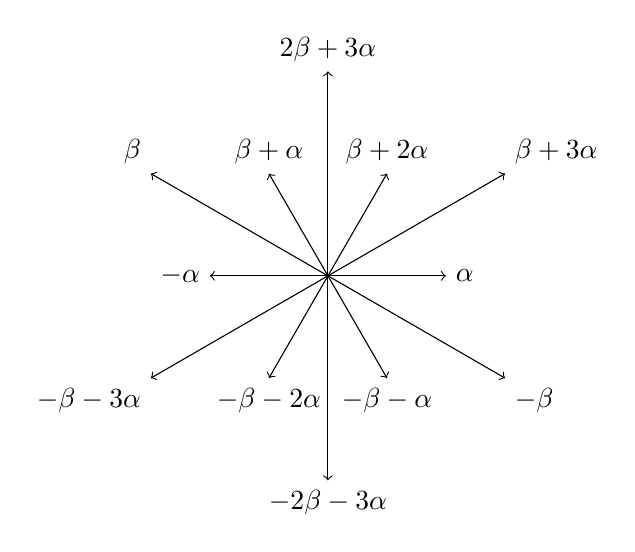
\begin{tikzpicture}[scale = 1.5]
    \foreach \ang in {60, 120, ..., 360}{
      \draw[->] (0,0) -- (\ang:1);
      \draw[->] (0,0) -- (\ang + 30 : 1.732); % 1.732 = sqrt(3)
    }
    \node[anchor=west]        at (0:1)        {$\alpha$};
    \node[anchor=south west]  at (30:1.732)   {$\beta + 3 \alpha$};
    \node[anchor=south]       at (60:1)       {$\beta + 2 \alpha$};
    \node[anchor=south]       at (90:1.732)   {$2 \beta + 3 \alpha$};
    \node[anchor=south]       at (120:1)      {$\beta + \alpha$};
    \node[anchor=south east]  at (150:1.732)  {$\beta$};
    \node[anchor=east]        at (180:1)      {$-\alpha$};
    \node[anchor=north east]  at (210:1.732)  {$-\beta - 3 \alpha$};
    \node[anchor=north]       at (240:1)      {$-\beta - 2 \alpha$};
    \node[anchor=north]       at (270:1.732)  {$-2 \beta - 3 \alpha$};
    \node[anchor=north]       at (300:1)      {$-\beta - \alpha$};
    \node[anchor=north west]  at (330:1.732)  {$-\beta$};
  \end{tikzpicture}
  \end{center}
  This root system is crystallographic and can hence be understood as a root system over an arbitrary field~$\kf$.
  To see how this resulting~{\rootsystem{$\kf$}} looks like we choose a basis~$\alpha$,~$\beta$ of~$\Real^2$ as indicated above.
  Then every root is a linear combination of~$\alpha$,~$\beta$ with integer coefficients.
  Applying the above constructions (restriction of scalars~$\Real \to \Rational$ followed by extension of scalars~$\Rational \to \kf$) we arrive at a~{\rootsystem{$\kf$}}~$R$ of rank~$2$ in a vector space~$V$ with basis~$\alpha$,~$\beta$ such that
  \[
    R
    =
    \Bigl\{
      \pm \alpha,
      \pm (\beta + 3 \alpha),
      \pm (\beta + 2 \alpha),
      \pm (2 \beta + 3 \alpha),
      \pm (\beta + \alpha),
      \pm \beta
    \Bigr\} \,.
  \]
  The reflection~$s_{\gamma}$ for~$\gamma \in R$ is in the picture given by the orthogonal reflection at the line that is orthogonal to~$\gamma$.
  With respect to the basis~$\alpha$,~$\beta$ of~$V$ these reflections can be expressed by the following matrices:
  \begin{alignat*}{3}
    s_\alpha
    &\equiv
    \begin{bmatrix*}[r]
      -1  & 3 \\
       0  & 1
    \end{bmatrix*} \,,
    &
    \quad
    s_{\beta + 3 \alpha}
    &\equiv
    \begin{bmatrix*}[r]
      -2 & 3 \\
      -1 & 2
    \end{bmatrix*} \,,
    &
    \quad
    s_{\beta + 2 \alpha}
    &\equiv
    \begin{bmatrix*}[r]
      -1  & 0 \\
      -1  & 1
    \end{bmatrix*} \,,
  \\
    s_{2 \beta + 3 \alpha}
    &\equiv
    \begin{bmatrix*}[r]
      1 & -3 \\
      0 & -1
    \end{bmatrix*} \,,
    &
    \quad
    s_{\beta + \alpha}
    &\equiv
    \begin{bmatrix*}[r]
      2 & -3 \\
      1 & -2 
    \end{bmatrix*} \,,
    &
    \quad
    s_\beta
    &\equiv
    \begin{bmatrix*}[r]
      1 &  0 \\
      1 & -1
    \end{bmatrix*} \,.
  \end{alignat*}
  We denote this root system by~$\rootG_2$.
  
  To determine the Weyl group of~$\rootG_2$ we may, by the above discussions, consider the starting case~$\kf = \Real$ with~$s_\gamma$ being the orthogonal reflection as explained above.
  We may draw the lines at which we reflect together with a hexagon into the following picture:
  \begin{center}
  \begin{tikzpicture}[scale = 1.5]
    \foreach \ang in {30, 60, ..., 360}{
      \draw[-, dashed] (0,0) -- (\ang:2);
    }
    \draw (0:1.5) -- (60:1.5) -- (120:1.5) -- (180:1.5) -- (240:1.5) -- (300:1.5) -- cycle;
  \end{tikzpicture}
  \end{center}
  We see from this picture that the Weyl group~$\Weyl(\rootG_2)$, which is generated by the reflection at these lines, is precisely the dihedral group of the hexagon,~$\dihedral_6$.
\end{example}





\subsection{Coroots and Duality of Root Systems}


\begin{definition}
  Let~$R$ be a root system in a~{\vectorspace{$\kf$}}~$V$.
  Let~$W$ be another~{\vectorspace{$\kf$}} and let~$\pair{-,-} \colon V \times W \to \kf$ be a non-degenerate bilinear form.
  For every root~$\alpha \in R$ there exists by \cref{reflections using duality} a unique element~$\check{\alpha} \in W$ such that the reflection~$s_\alpha$ is given by~$s_\alpha(v) = v - \pair{v, \check{\alpha}} \alpha$ for every~$v \in V$.
  The element~$\check{\alpha}$ is the \defemph{coroot} associated to~$\alpha$ (with respect to the pairing~$\pair{-,-}$).
  The set of coroots is denoted by~$\check{R} = \{\check{\alpha} \suchthat \alpha \in R\}$.
  (This is a subset of~$W$.)
\end{definition}


\begin{remark}
  If~$\alpha, \beta \in R$ are proportional roots, i.e.\ if~$\beta = \lambda \alpha$ for some scalar~$\lambda$ (necessarily nonzero) then~$s_\alpha = s_\beta$ and then also~$\check{\beta} = \lambda^{-1} \check{\alpha}$.
  In particular~$\check{(-\alpha)} = -\check{\alpha}$.
  But if~$\alpha, \beta \in R$ are two roots whose sum~$\alpha + \beta$ is again a root, then in general~$\check{(\alpha + \beta)} = \check{\alpha} + \check{\beta}$.
\end{remark}


% TODO: Give a counterexample that show that check does not have to be compatible with sums.


\begin{proposition}
  \label{dual root system}
  Let~$R$ be a root system in a~{\vectorspace{$\kf$}}~$V$ and let~$\pair{-,-} \colon V \times W \to \kf$ be a non-degenerate bilinear form.
  \begin{enumerate}
    \item
      \label{coroots are a root system}
      The set of coroots~$\check{R}$ is a root system in~$W$.
    \item
      \label{description of dual reflections}
      For every root~$\alpha \in R$ the reflections~$s_{\check{\alpha}}$ and~$s_\alpha$ are related by~$s_{\check{\alpha}} = s_\alpha^*$, and the reflection~$s_{\check{\alpha}}$ is given on coroots by~$s_{\check{\alpha}}(\check{\beta}) = \check{s_\alpha(\beta)}$ for every~$\beta \in R$.
    \item
      \label{antiisomorphism of weyl groups}
      The algebra anti-isomorphism~$\End(V) \to \End(W)$ given by~$f \mapsto f^*$ restricts to a group anti-isomorphism~$\Weyl(R) \to \Weyl(\check{R})$.
  \end{enumerate}
\end{proposition}


\begin{proof}
  It follows for every root~$\alpha \in R$ from~$\pair{\alpha, \check{\alpha}} = 2$ that~$\check{\alpha} \neq 0$ whence~$0 \notin \check{R}$.
  Suppose that~$W$ were not spanned by~$\check{R}$.
  Then~$\gen{\check{R}}_{\kf}$ is a proper subspace of~$W$ whence its orthogonal~$\gen{\check{R}}_{\kf}^\perp$ is a nonzero linear subspace of~$V$.
  There hence exists some nonzero vector~$v \in V$ with~$\pair{v, \check{\alpha}} = 0$ for every~$\alpha \in R$.
  This then means that the nonzero vector~$v$ is fixed by every reflection~$s_\alpha$ with~$\alpha \in R$, and hence fixed by every element of the Weyl group~$\Weyl(R)$.
  But this contradicts \cref{weyl groups fixes no line}.
  We therefore find that~$W$ is spanned by~$\check{R}$.
  
  To finish proving part~\ref*{coroots are a root system} and to prove part~\ref*{description of dual reflections} we need to show that for every root~$\alpha \in R$ the linear map~$s_\alpha^* \colon W \to W$ is a reflection with~$s_\alpha^*(\check{\alpha}) = -\check{\alpha}$,~$s_\alpha^*(\check{R}) \subseteq \check{R}$ and~$s_\alpha^*(\check{\beta}) = \check{s_\alpha(\beta)}$.
  That~$s_\alpha^*$ is again a reflection follows from part~\ref*{dual reflections} of \cref{properties of reflections}.
  The next two conditions follow from the last condition~$s_\alpha^*(\check{\beta}) = \check{s_\alpha(\beta)}$ because~$\check{(-\alpha)} = -\check{\alpha}$ and~$\check{s_\alpha(\beta)} \in R$.
  
  For this last condition we observe that
  \begin{align}
    s_{s_\alpha(\beta)}
    &=
    s_\alpha \circ s_\beta \circ s_\alpha^{-1}
    \label{pulling apart}
    \\
    &=
    s_\alpha \circ s_{\beta, \check{\beta}} \circ s_\alpha^{-1}
    \notag
    \\
    &=
    s_{s_\alpha(\beta), s_\alpha^{-*}(\check{\beta})}
    \label{pulling together again}
    \\
    &=
    s_{s_\alpha(\beta), s_{\check{\alpha}}(\check{\beta})}
    \label{simplifying index}
  \end{align}
  The equality~\eqref{pulling apart} follows from \cref{reflection of conjugated root}, equality~\eqref{pulling together again} follows from part~\ref*{conjugation of reflection} of \cref{properties of reflections}, and equality~\eqref{simplifying index} follows from part~\ref*{dual reflections} of \cref{properties of reflections} because
  \[
    s_\alpha^{-*}(\check{\beta})
    =
    (s_\alpha^{-1})^*(\check{\beta})
    =
    s_\alpha^*(\check{\beta})
    =
    s_{\check{\alpha}}(\check{\beta}) \,.
  \]
  The above equality~$s_{s_\alpha(\beta)} = s_{s_\alpha(\beta), s_{\check{\alpha}}(\check{\beta})}$ shows that~$s_{\check{\alpha}}(\check{\beta})$ satisfies the defining property of the coroot~$\check{s_\alpha(\beta)}$.
  
  Part~\ref*{antiisomorphism of weyl groups} follows from part~\ref*{description of dual reflections} because the given anti-isomorphism of~{\algebras{$\kf$}}~$\End(V) \to \End(W)$ restricts to an anti-isomorphism of groups~$\GL(V) \to \GL(W)$ which maps the generators~$s_\alpha$ of the Weyl group~$\Weyl(R)$ (with~$\alpha \in R$) onto the generators~$s_\alpha^* = s_{\check{\alpha}}$ of the Weyl group~$\Weyl(\check{R})$.
\end{proof}


\begin{lemma}
  \label{double duality of root systems}
  Let~$R$ be a root system in a~{\vectorspace{$\kf$}}~$V$.
  Let~$W$ be another~{\vectorspace{$\kf$}} and let~$\pair{-,-} \colon V \times W \to \kf$ be a non-degenerate bilinear form.
  For every root~$\alpha \in R$ let~$\dcheck{\alpha} \in V$ be the coroot of~$\check{\alpha} \in \check{R}$ with respect to~$\pair{-,-}$.%
  \footnote{Strictly speaking we do not use~$\pair{-,-}$ to go from~$\check{\alpha}$ to~$\dcheck{\alpha}$ but instead the twisted version of~$\pair{-,-}$ given by the composition~$W \times V \xto{\text{swap}} V \times W \xto{\pair{-,-}} \kf$.}
  Then~$\dcheck{\alpha} = \alpha$ and overall~$\dcheck{R} = R$.
\end{lemma}


\begin{proof}
  Let~$\alpha \in R$ be any root.
  For the associated coroot~$\check{\alpha}$ its reflection~$s_{\check{\alpha}}$ is according to \cref{dual root system} given by~$s_{\check{\alpha}} = s_\alpha^*$.
  The reflection fo the associated double coroot~$\dcheck{\alpha}$ is hence given by~$s_{\dcheck{\alpha}} = s_{\check{\alpha}}^* = s_\alpha^{**} = s_\alpha$.
  It follows from part~\ref*{dual reflections} of \cref{properties of reflections} that the double coroot~$\dcheck{\alpha}$, i.e.\ the unique element~$\dcheck{\alpha} \in V$ with~$s_{\check{\alpha}}(w) = w - \pair{\dcheck{\alpha}, w} \check{\alpha}$ for every~$w \in W$, is given by~$\alpha$ itself.
  Whence~$\dcheck{\alpha} = \alpha$.
\end{proof}


\begin{corollary}
  \label{root to dual root is bijective}
  Let~$R$ be a root system in a~{\vectorspace{$\kf$}}~$V$.
  Let~$W$ be another~{\vectorspace{$\kf$}} and let~$\pair{-,-} \colon V \times W \to \kf$ be a non-degenerate bilinear form.
  Then the map~$R \to \check{R}$ given by~$\alpha \mapsto \check{\alpha}$ is a bijection with inverse given by~$\check{\alpha} \mapsto \dcheck{\alpha} = \alpha$.
  \qed
\end{corollary}


\begin{lemma}
  \label{uniqueness of dual}
  Let~$R$ be a root system in a~{\vectorspace{$\kf$}}~$V$.
  Let~$W_1$ and~$W_2$ be two~{\vectorspaces{$\kf$}} with non-degenerate bilinear forms~$\pair{-,-}_1 \colon V \times W_1 \to \kf$ and~$\pair{-,-}_2 \colon V \times W_2 \to \kf$.
  Let~$\check{R_1}$ and~$\check{R_2}$ be the resulting root systems of coroots in~$W_1$ and~$W_2$.
  Let~$f \colon W_1 \to W_2$ be the unique linear map with
  \begin{equation}
    \label{defining equation for isomorphism of duals}
    \pair{v, w_1}
    =
    \pair{v, \spacing f(w_1)}
  \end{equation}
  for all~$v \in V$ and~$w_1 \in W_1$.
  Then~$f$ is an isomorphism of root systems~$(\check{R_1}, W_1) \to (\check{R_2}, W_2)$.
\end{lemma}


\begin{proof}
  The non-degenerate bilinear forms~$\pair{-,-}_1$ and~$\pair{-,-}_2$ correspond to isomorphisms of vector spaces~$\varphi_1 \colon W_1 \to V^*$ and~$\varphi_2 \colon W_2 \to V^*$ given by~$\varphi_1(w_1) = \pair{-, w_1}_1$ and~$\varphi_2(w_2) = \pair{-, w_2}_2$.
  The proposed linear map~$f \colon W_1 \to W_2$ is precisely the composition~$f = \varphi_2^{-1} \circ \varphi_1$.
  It is is particular an isomorphism of vector spaces.
  It follows from~\eqref{defining equation for isomorphism of duals} that~$f(\check{\alpha}) = \check{\alpha}$ for every~$\alpha \in R$.
  It follows from \cref{root to dual root is bijective} that the linear isomorphism~$f$ maps the root system~$\check{R_1}$ bijectively into the root system~$\check{R_2}$ and is therefore an isomorphism of root systems as asserted.
\end{proof}


\begin{definition}
  Let~$R$ be a root system in a~{\vectorspace{$\kf$}}~$V$.
  Let~$W$ be another vector space and let~$\pair{-,-} \colon V \times W \to \kf$ be a non-degenerate bilinear form.
  The root system~$\check{R}$ in~$W$ is the \defemph{dual \textup(root system\textup)} of~$R$.
\end{definition}


\begin{remark}
  Let~$R$ be a root system in a~{\vectorspace{$\kf$}}~$V$.
  \begin{enumerate}
    \item
      \Cref{uniqueness of dual} shows that the dual of the root system~$R$ does up to (sensible) isomorphism not depend on the choice of non-degenerate bilinear form~$\pair{-,-}$.
      
      As a consequence of this we will often talk about the coroots~$\check{\alpha}$ for~$\alpha \in R$ without specifying the choice of non-degenerate bilinear form~$\pair{-,-}$.
    \item
      Many references define the dual of a root system~$R$ only for a specific choice of non-degenerate bilinear form~$\pair{-,-} \colon V \times W \to \kf$.
      As an example, in \cite[18]{tauvel_yu} and in the lecture (which these notes are based on) coroots and the dual root system is only defined for~$W = V^*$ and~$\pair{-,-}$ the standard pairing.
    \item
      \Cref{double duality of root systems} shows that a root system~$R$ and its dual~$\check{R}$ are indeed dual to each other, in the sense that~$\dcheck{R} = R$ and even~$\dcheck{\alpha} = \alpha$ for every roots~$\alpha \in R$.
  \end{enumerate}
\end{remark}


\begin{example}
  \label{explicit coroots for standard root systems}
  We endow the vector space~$\kf^n$ with the standard pairing~$\pair{-,-} \colon \kf^n \times \kf^n \to \kf$ given by~$\pair{x,y} = \sum_{i=1}^n x_i y_i$.
  In the following we will compute explicitely the coroots and dual root systems of the root systems~$\rootA_n$,~$\rootB_n$,~$\rootC_n$ and~$\rootD_n$.
  \begin{enumerate}
    \item
      We begin with the root system~$\rootB_n$ in~$\kf^n$.
      Recall that
      \[
        \rootB_n
        =
        \{
          \pm e_i
        \suchthat
          i = 1, \dotsc, n
        \}
        \cup
        \{
          \pm e_i \pm e_j
        \suchthat
          1 \leq i \neq j \leq n
        \} \,.
      \]
      By using the explicit descriptions of the reflections~$s_\alpha$ for~$\alpha \in \rootB_n$ we can calculate the coroots with respect to~$\pair{-,-}$.
      \begin{itemize}
        \item
          The reflection~$s_{e_i}$ is given by mapping~$e_i \mapsto -e_i$ and~$e_j \mapsto e_j$ for~$j \neq i$.
          The reflection~$s_{e_i}$ is therefore given by
          \[
            s_{e_i}(x)
            =
            x - 2 x_i e_i
            =
            x - \pair{x, 2 e_i} e_i \,.
          \]
          This shows that~$\check{e_i} = 2 e_i$.
          Then also~$\check{(-e_i)} = -\check{e_i} = -2 e_i$.
        \item
          The reflection~$s_{e_i - e_j}$ is on standard basis vectors given by
          \[
            e_i \mapsto e_j \,,
            \quad
            e_j \mapsto e_i \,,
            \quad
            e_k \mapsto e_k \,,
          \]
          where~$k \neq i,j$.
          This means that
          \[
            e_i
            \mapsto
            e_i - 1 \cdot (e_i - e_j) \,,
            \quad
            e_j
            \mapsto
            e_j - (-1) \cdot (e_i - e_j) \,,
            \quad
            e_k
            \mapsto
            e_k - 0 \cdot (e_i - e_j) \,.
          \]
          We see from this that the linear functional~$\pair{-, \check{(e_i - e_j)}} \colon \kf^n \to \kf$ is given on standard basis vectors by
          \[
            e_i \mapsto 1 \,,
            \quad
            e_j \mapsto -1 \,,
            \quad
            e_k
            \mapsto
            0 \,.
          \]
          This means that~$\check{(e_i - e_j)} = e_i - e_j$.
          It also follows that
          \[
            \check{(-e_i + e_j)}
            =
            -\check{(e_i - e_j)}
            =
            -(e_i - e_j)
            =
            -e_i + e_j \,.
          \]
        \item
          We proceed similarly for the coroot~$\check{(e_i + e_j)}$:
          The reflection~$s_{e_i + e_j}$ is on standard basis vectors given by
          \[
            e_i
            \mapsto
            -e_j \,,
            \quad
            e_j
            \mapsto
            -e_i \,,
            \quad
            e_k
            \mapsto
            e_k
          \]
          for~$k \neq i,j$.
          This means that
          \[
            e_i
            \mapsto
            e_i - 1 \cdot (e_i + e_j) \,,
            \quad
            e_j
            \mapsto
            e_j - 1 \cdot (e_i + e_j) \,,
            \quad
            e_k
            \mapsto
            e_k - 0 \cdot (e_i + e_j) \,.
          \]
          The linear functional~$\pair{-, \check{(e_i + e_j)}} \colon \kf^n \to \kf$ is therefore given by
          \[
            e_i
            \mapsto
            1 \,,
            \quad
            e_j
            \mapsto
            1 \,,
            \quad
            e_k
            \mapsto
            0
          \]
          which tells us that~$\check{(e_i + e_j)} = e_i + e_j$.
          Then also
          \[
            \check{(- e_i - e_j)}
            =
            -\check{(e_i + e_j)}
            =
            -(e_i + e_j)
            =
            - e_i - e_j \,.
          \]
      \end{itemize}
      We see that overall
      \[
        \check{\rootB_n}
        =
        \{
          2 e_i
        \suchthat
          i = 1, \dotsc, n
        \}
        \cup
        \{
          \pm e_i \pm e_j
        \suchthat
          1 \leq i \neq j \leq n
        \} \,.
      \]
      This is precisely the root system~$\rootC_n$.
      We have hence shown that~$\check{\rootB_n} = \rootC_n$.
    \item
      We now also find that
      \[
        \check{\rootC_n}
        =
        \dcheck{\rootB_n}
        =
        \rootB_n \,.
      \]
      More precisely,~$\check{(2 e_i)} = e_i$ for every~$i = 1, \dotsc, n$ and~$\check{(\pm e_i \pm e_j)} = \pm e_i \pm e_j$ for all~$1 \leq i \neq j \leq n$.
    \item
      Recall that the root system~$\rootD_n$ is given by
      \[
        \rootD_n
        =
        \{
          \pm e_i \pm e_j
        \suchthat
          1 \leq i \neq j \leq n \,.
        \}
      \]
      We can reuse the above calculations to find that~$\check{(\pm e_i \pm e_j)} = \pm e_i \pm e_j$ for all~$1 \leq i \neq j \leq n$.
      We hence find that~$\check{\rootD_n} = \rootD_n$.
    \item
      The root system~$\rootA_n$ is given by
      \[
        \rootA_n
        =
        \{
          e_i - e_j
        \suchthat
          1 \leq i \neq \leq j \leq n
        \} \,,
      \]
      and it is a root system in the vector space
      \[
        V
        =
        \{
          (x_1, \dotsc, x_n) \in \kf^n
        \suchthat
          x_1 + \dotsb + x_n = 0
        \} \,.
      \]
      The restriction of the standard pairing~$\pair{-,-}$ to the linear subspace~$V$ of~$\kf^n$ is again non-degenerate since the orthogonal of~$V$ is given by~$V^\perp = \gen{(1, \dotsc, 1)}_{\kf}$ and thus~$\kf^n = V \oplus V^\perp$.
      We denote the restriction of~$\pair{-,-}$ to~$V$ again by~$\pair{-,-}$.
      
      The reflection~$s_{e_i - e_j}$ is the restriction of the reflection~$s_{ij} \colon \kf^n \to \kf^n$ given by
      \[
        e_i
        \mapsto
        e_j \,,
        \quad
        e_j
        \mapsto
        e_i \,,
        \quad
        e_k
        \mapsto
        e_k
      \]
      for~$k \neq i,j$.
      We have seen in the previous calculations that the reflections~$s_{ij}$ are given by
      \[
        s_{ij}(x)
        =
        x - \pair{x, e_i - e_j} (e_i - e_j)
      \]
      for every~$x \in \kf^n$.
      For the reflections~$s_{e_i - e_j}$ the same formula holds (as they are restrictions of the reflections~$s_{ij}$) and we hence find that~$\check{(e_i - e_j)} = e_i - e_j$.
      This shows in particular that~$\check{\rootA_n} = \rootA_n$.0
  \end{enumerate}
\end{example}


\begin{lemma}
  \label{formula for orthogonal coroots}
  Let~$R$ be a root system in a~{\vectorspace{$\kf$}} and let~$\inner{-,-} \colon V \times V \to \kf$ be a non-degenerate symmetric bilinear form.
  Suppose that for every root~$\alpha \in R$ the reflection~$s_\alpha$ is an isometry with respect to~$\inner{-,-}$. 
  Then~$\inner{\alpha, \alpha} \neq 0$ for every root~$\alpha \in R$, and the associated coroot is given by
  \[
    \check{\alpha}
    =
    \frac{2 \alpha}{\inner{\alpha, \alpha}} \,.
  \]
\end{lemma}


\begin{proof}
  
  It follows from \cref{orthogonal reflections are orthogonal reflections} that~$\inner{\alpha, \alpha} \neq 0$ and that the reflection~$s_\alpha$ is given by
  \[
    s_\alpha(v)
    =
    v - 2 \frac{\inner{v,\alpha}}{\inner{\alpha, \alpha}} \alpha
  \]
  for every~$v \in V$.
  We may rewrite this expression as
  \[
    s_\alpha(v)
    =
    v - \inner*{v, \frac{2 \alpha}{\inner{\alpha, \alpha}} } \alpha \,,
  \]
  which gives the asserted form of~$\check{\alpha}$.
\end{proof}


\begin{examples}
  Let again~$\inner{-,-}$ be the standard symmetric bilinear form on~$\kf^n$, still given by~$\inner{x,y} = \sum_{i=1}^n x_i y_i$.
  Let~$V = \{ (x_1, \dotsc, x_n) \in \kf^n \suchthat x_1 + \dotsb + x_n = 0 \}$ be the linear subspace of~$\kf^n$ in which~$\rootA_n$ is a root system.
  We denote the restriction of~$\inner{-,-}$ to~$V$ again by~$\inner{-,-}$.
  
  We have seen in \cref{standard root systems have isometric reflections} that for the root systems~$\rootA_n$,~$\rootB_n$,~$\rootC_n$ and~$\rootD_n$ the reflections~$s_\alpha$, for~$\alpha$ some root, are isometries with respect to~$\inner{-,-}$..
  We can therefore apply \cref{formula for orthogonal coroots} to calculate the coroots a second time:  
  We have
  \[
    \inner{\pm e_i,  \pm e_i}
    =
    1 \,,
    \quad
    \inner{\pm 2 e_i, \pm 2 e_i}
    =
    4 \,,
    \quad
    \inner{\pm e_i \pm e_j, \pm e_i \pm e_j}
    =
    2
  \]
  where the signs in the first argument are choosen arbitrary but the signs in the second argument are as in the first argument.
  It follows that
  \begin{align*}
    \check{(\pm e_i)}
    &=
    \frac{2}{\inner{\pm e_i,  \pm e_i}}
    \cdot
    (\pm e_i)
    =
    \frac{2}{1}
    \cdot
    (\pm e_i)
    =
    \pm 2 e_i \,,
    \\[0.5em]
    \check{(\pm 2 e_i)}
    &=
    \frac{2}{\inner{\pm 2 e_i,  \pm 2 e_i}}
    \cdot
    (\pm 2 e_i)
    =
    \frac{2}{4}
    \cdot
    (\pm 2 e_i)
     =
    \pm e_i \,,
    \\[0.5em]
    \check{(\pm e_i \pm e_j)}
    &=
    \frac{2}{\inner{\pm e_i \pm e_j,  \pm e_i \pm e_j}}
    \cdot
    (\pm e_i \pm e_j)
    =
    \frac{2}{2}
    \cdot
    (\pm e_i \pm e_j)
    =
    \pm e_i \pm e_j \,.
  \end{align*}
  These are indeed the same results as in \cref{explicit coroots for standard root systems}.
\end{examples}


% TODO: G2 selfdual; how to prove?


\begin{definition}
  Let~$R$ be a root system in a~{\vectorspace{$\kf$}}.
  By \cref{reflected vector is a linear combination} there exists for any two roots~$\alpha, \beta \in R$ a scalar~$c_{\alpha \beta} \in \kf$ with~$s_{\beta}(\alpha) = \alpha - c_{\alpha \beta} \beta$.
  The numbers~$c_{\alpha \beta}$ are the \defemph{Cartan numbers}.
\end{definition}


\begin{lemma}
  \label{properties via cartan numbers}
  \leavevmode
  \begin{enumerate}
    \item
      \label{crystallographic via cartan numbers}
      A root system~$R$ is crystallographic if and only if~$c_{\alpha \beta} \in \Integer$ for any two roots~$\alpha, \beta \in R$.
    \item
      Let~$\Lf/\kf$ be a field extension and let~$R$ be an~{\rootsystem{$\Lf$}}.
      Then~$R$ is definable over~$\kf$ if and only if~$c_{\alpha \beta} \in \kf$ for any two roots~$\alpha, \beta \in R$.
    \qedhere
  \end{enumerate}
\end{lemma}


\begin{remark}
  For the crystallographic root system~$R$ the Cartan numbers are also known as \defemph{Cartan integers}.
\end{remark}


\begin{lemma}
  \label{cartan numbers via coroots}
  Let~$R$ be a root system in a~{\vectorspace{$\kf$}}~$V$.
  The Cartan numbers of~$R$ are given by~$c_{\alpha \beta} = \pair{\alpha, \check{\beta}}$ for any two roots~$\alpha, \beta \in R$.
\end{lemma}


\begin{proof}
  We have~$s_\beta(\alpha) = \alpha - \pair{\alpha, \check{\beta}} \beta$ whence~$\pair{\alpha, \check{\beta}}$ satisfies the defining propery of~$c_{\alpha \beta}$.
\end{proof}


\begin{corollary}
  \leavevmode
  \begin{enumerate}
    \item
      A root system~$R$ is crystallographic if and only if~$\pair{\alpha, \check{\beta}} \in \Integer$ for any two roots~$\alpha, \beta \in R$.
    \item
      Let~$\Lf/\kf$ be a field extension.
      An~{\rootsystem{$\Lf$}}~$R$ is definable over~$\kf$ if and only if~$\pair{\alpha, \check{\beta}} \in \kf$ for any two roots~$\alpha, \beta \in R$.
  \end{enumerate}
\end{corollary}


\begin{proof}
  This is a reformulation of \cref{properties via cartan numbers} via \cref{cartan numbers via coroots}.
\end{proof}


\begin{corollary}
  Let~$R$ be a root system.
  The Cartan numbers for~$R$ and for its dual root system~$\check{R}$ satisfy for two roots~$\alpha, \beta \in R$ the equality
  \[
    c_{\alpha \beta}
    =
    c_{\check{\beta} \check{\alpha}} \,.
  \]
\end{corollary}


\begin{proof}
  Let~$\pair{-,-} \colon V \times W \to \kf$ be a non-degenerate bilinear form.
  Then
  \[
    c_{\alpha \beta}
    =
    \pair{\alpha, \check{\beta}}
    \quad\text{and}\quad
    c_{\check{\beta} \check{\alpha}}
    =
    \pair{\dcheck{\alpha}, \check{\beta}} \,.
  \]
  The assertion follows since~$\dcheck{\alpha} = \alpha$.
\end{proof}


% TODO: Extension and restriction of fields for coroots.


\begin{proposition}
  Let~$\Lf/\kf$ be a field extension.
  \begin{enumerate}
    \item
      Let~$V$ be a root system in a~{\vectorspace{$\kf$}}~$V$ and let~$\pair{-,-} \colon V \times W \to \kf$ be a non-degenerate bilinear form.
      The bilinear form~$\pair{-,-}$ extends uniquely to an~{\bilinear{$\Lf$}} form~$\pair{-,-}_\Lf \colon V_{\Lf} \times W_{\Lf} \to \Lf$.
      This bilinear form is again non-degenerate, and the coroots of the extended root system~$R_{\Lf}$ with respect to~$\pair{-,-}_{\Lf}$ satisfy
      \[
        \check{(1 \tensor \alpha)}
        =
        1 \tensor \check{\alpha}
      \]
      for every~$\alpha \in R$.
      As a consequence~$\check{(R_{\Lf})} = (\check{R})_{\Lf}$.
    \item
      Let~$R$ be a root system in an~{\vectorspace{$\Lf$}}~$V$ and let~$\pair{-,-} \colon V \times W \to \Lf$ be a non-degenerate bilinear form.
      Suppose that the root system~$R$ is definable over~$\kf$.
      Then the dual root system~$\check{R}$ is also definable over~$\kf$.
      The~{\bilinear{$\Lf$}} form~$\pair{-,-}$ restricts to a well-defined~{\bilinear{$\kf$}} form~$\restrict{\pair{-,-}}{\kf} \colon \restrict{V}{\kf} \times \restrict{W}{\kf} \to \kf$.
      This restricted bilinear form is again non-degenerate and the coroot of~$\alpha \in R$ with respect to~$\restrict{\pair{-,-}}{\kf}$ coincides with the coroot with respect to~$\pair{-,-}$.
      In particular~$\check{(\restrict{R}{\kf})} = \restrict{\check{R}}{\kf}$.
  \end{enumerate}
\end{proposition}





\section{Euclidian Root Systems}


\begin{definition}
  A real root system~$(R, V)$ is \defemph{euclidian} if~$V$ is a real inner product space and the reflections~$s_\alpha$ for~$\alpha \in R$ are isometries.
\end{definition}

% TODO: Remark regarding the terminology.





\subsection{Bases and Positive Roots}


\begin{definition}
  Let~$R$ be a root system in a~{\vectorspace{$\kf$}}~$V$.
  \begin{enumerate}
    \item
      A subset~$\Pi \subseteq R$ is a \defemph{positive system} if
      \begin{enumerate}
        \item
          for every root~$\alpha \in R$ precisely one of the two roots~$\alpha$ and~$-\alpha$ is contained in~$R$, and
        \item
          for any two roots~$\beta_1, \beta_2 \in \Pi$ also~$\beta_1 + \beta_2 \in \Pi$.
      \end{enumerate}
      The elements of~$\Pi$ are \defemph{positive roots}, the elements of~$-\Pi$ are \defemph{negative roots}.
      An positive root~$\alpha \in \Pi$ is \defemph{decomposable} if it can be written as~$\alpha = \beta_1 + \beta_2$ for two positive roots~$\beta_1, \beta_2 \in \Pi$.
      Otherwise it is \defemph{indecomposable}.
    \item
      A subset~$\Delta \subseteq R$ is a \defemph{basis} of~$R$ if 
      \begin{enumerate}
        \item
          $\Delta$ is a vector space basis of~$V$, and
        \item
          for every root~$\beta \in R$ the linear combination~$\beta = \sum_{\alpha \in \Delta} k_\alpha \alpha$ satisfies~$k_\alpha \in \Integer_{\geq 0}$ for every~$\alpha \in \Delta$ or~$k_\alpha \in \Integer_{\leq 0}$ for every~$\alpha \in \Delta$.
      \end{enumerate}
      The elements of~$\Delta$ are~\defemph{simple roots}.
  \end{enumerate}
\end{definition}


\begin{proposition}
  Let~$R$ be a reduced crystallographic root system.
  \begin{enumerate}
    \item
      Let~$\Delta$ be a basis of~$R$.
      Then
      \[
        \Pi
        =
        \left\{
          \beta \in R
        \suchthat*
          \text{$\beta = \sum_{\alpha \in \Delta} k_\alpha \alpha$ with~$\alpha \in \Integer_{\geq 0}$ for every~$\alpha \in \Delta$}
        \right\} \,.
      \]
      is a positive system for~$R$.
    \item
      Let~$\Pi$ be a positive system for~$R$.
      Then
      \[
        \Delta
        =
        \{
          \text{$\alpha \in \Pi$ is indecomposable}
        \}
      \]
      is a basis of~$R$.
    \item
      The above constructions give a {\onetoone} correspondence
      \[
        \{
          \text{positive systems~$\Pi \subseteq R$}
        \}
        \longonetoone
        \{
          \text{bases~$\Delta \subseteq R$}
        \} \,.
      \]
  \end{enumerate}
\end{proposition}


\begin{proof}
  We will show this later.
\end{proof}








% \section{Coroots}
% 
% \begin{lemma}
%   \label{properties of coroots}
%   Let~$R$ be a root system in a~{\vectorspace{$\kf$}}~$V$.
%   \begin{enumerate}
%     \item
%       If~$\alpha \in R$ is a root and~$\lambda \neq 0$ such that~$\lambda \alpha$ is again a root then~$\check{(\lambda \alpha)} = \lambda^{-1} \check{\alpha}$.
%     \item
%       For all~$\alpha, \beta \in R$,~$\check{s_\alpha(\beta)} = s_{\check{\alpha}, \alpha}(\check{\beta})$.
%   \end{enumerate}
% \end{lemma}
% 
% 
% \begin{proof}
%   \leavevmode
%   \begin{enumerate}
%     \item
%       We have~$\pair{\lambda \alpha, \lambda^{-1} \check{\alpha}} = \pair{\alpha, \check{\alpha}} = 2$ whence the reflection~$s_{\lambda \alpha, \spacing \lambda^{-1} \alpha}$ is well-defined.
%       It follows from part~\ref*{uniqueness of reflection parametrization} of \cref{regarding general reflections} that~$s_{\lambda \alpha, \spacing \lambda^{-1} \check{\alpha}} = s_{\alpha, \check{\alpha}}$, which shows that~$s_{\lambda \alpha, \spacing \lambda^{-1} \check{\alpha}}$ leaves~$R$ invariant.
%       Together this shows that~$\lambda^{-1} \check{\alpha}$ satisfies the defining properties of~$\check{(\lambda \alpha)}$.
%     \item
%       We have
%       \[
%         \pair{s_\alpha(\beta), s_{\check{\alpha}, \alpha}(\check{\beta})}
%         =
%         \pair{s_\alpha(\beta), s_\alpha^*(\check{\beta})}
%         =
%         \pair{s_\alpha^2(\beta), \check{\beta}}
%         =
%         \pair{\beta, \check{\beta}}
%         =
%         2
%       \]
%       where we use that~$s_{\check{\alpha}, \alpha}= s_{\alpha, \check{\alpha}}^* = s_\alpha^*$ by \cref{properties of reflections}.
%       The reflection~$s_{[s_\alpha(\beta)], [s_{\check{\alpha}, \alpha}(\check{\beta})]}$ is therefore well-defined.%
%       \footnote{The brackets are only here for better readability and have no meaning on their own.}
%       We also see from \cref{properties of reflections} that
%       \[
%         s_{[s_\alpha(\beta)], [s_{\check{\alpha}, \alpha}(\check{\beta})]}
%         =
%         s_{[s_\alpha(\beta)], [s_\alpha^*(\check{\beta})]}
%         =
%         s_\alpha \circ s_\beta \circ s_\alpha^{-1} 
%         =
%         s_\alpha \circ s_\beta \circ s_\alpha \,.
%       \]
%       We see from this that the reflection~$s_{[s_\alpha(\beta)], [s_{\check{\alpha}, \alpha}(\check{\beta})]}$ leaves~$R$ invariant.
%       This shows that~$s_{\check{\alpha}, \alpha}(\check{\beta})$ satisfies the defining property of the coroot~$\check{s_\alpha(\beta)}$.
%     \qedhere
%   \end{enumerate}
% \end{proof}
% 
% 
% \begin{theorem}
%   \label{dual root system}
%   If~$R$ is a root system in a~{\vectorspace{$\kf$}}~$V$ then the set of coroots~$\check{R}$ is a root system in~$V^*$.
%   For every~$\alpha \in R$ the coroot of~$\check{\alpha}$, i.e.\ the element~$\dcheck*{\alpha} \in V^{**}$, is given by evaluation at~$\alpha$.
%   If~$R$ is reduced or crystallographic then the same holds for~$\check{R}$.
% \end{theorem}
% 
% 
% \begin{proof}
%   If~$0 \in \check{R}$ then~$\check{\alpha} = 0$ for some~$\alpha \in R$, which would contradict~$\pair{\alpha, \check{\alpha}} = 2$.
%   Thus~$0 \notin \check{R}$.
%   
%   The set of coroots~$\check{R}$ spans~$V^*$:
%   Otherwise the the span of~$\check{R}$ would a proper linear subspace of~$V^*$.
%   Then there would exists some nonzero~$v \in V$ with~$\pair{v, \varphi} = 0$ for every~$\varphi$ contained in this span.
%   Then in particular~$\pair{v, \check{\alpha}} = 0$ for every~$\alpha \in R$ and thus~$s_\alpha(v) = v$ for every~$\alpha \in R$.
%   Then~$w(v) = v$ for every~$w \in \Weyl(R)$, which would contradicts \cref{weyl group fixes no vector}.
%   Thus~$\check{R}$ spans~$V^*$
%   
%   For every~$\alpha \in R$ the proposed coroot of~$\check{\alpha} \in \check{R}$ is the element~$\dcheck*{\alpha} \in V^{**}$ given by evaluation at~$\alpha$.
%   Indeed,~$\pair{\check{\alpha}, \dcheck{\alpha}} = \pair{\alpha, \check{\alpha}} = 2$ and for every~$\beta \in R$,
%   \[
%     s_{\check{\alpha}, \dcheck{\alpha}}(\check{\beta})
%     =
%     s_{\check{\alpha}, \alpha}(\check{\beta})
%     =
%     \check{s(\beta)}
%     \in
%     \check{R}
%   \]
%   by \cref{properties of coroots}.
%   This shows that~$\check{R}$ is indeed a root system, with the coroot~$\dcheck*{\alpha} \in V^{**}$ of~$\check{\alpha}$ given by evaluation at~$\alpha$.
%   
%   Suppose that~$R$ is reduced, and that for some~$\alpha \in R$ some multiple~$\lambda \check{\alpha}$ is contained in~$R$.
%   Note that necessarily~$\lambda \neq 0$ since~$0 \notin \check{R}$.
%   Then also~$\lambda^{-1} \dcheck{\alpha} = \check{(\lambda\check{\alpha})} \in \dcheck{R}$ by \cref{properties of coroots}.
%   We know that under the natural isomorphism~$V \cong V^{**}$ the root system~$R$ corresponds to~$\dcheck{R}$;
%   more precisely,~$\alpha$ corresponds to~$\dcheck{\alpha}$.
%   It hence follows from~$\lambda^{-1} \dcheck*{\alpha} \in \dcheck{R}$ that~$\lambda^{-1} \alpha \in R$.
%   It follows that~$\lambda^{-1} = \pm 1$ and thus~$\lambda = \pm 1$ because~$R$ is reduced.
%   Thus the only multiples of~$\check{\alpha}$ contained in~$\check{R}$ are~$\check{\alpha}$ and~$-\check{\alpha}$, showing that~$\check{R}$ is again reduced.
%   
%   Suppose that~$R$ is crystallographic.
%   Then~$\pair{\check{\alpha}, \dcheck{\beta}} = \pair{\beta, \check{\alpha}} \in \Integer$ for all~$\alpha, \beta \in R$.
%   Thus~$\check{R}$ is again crystallographic.
% \end{proof}
% 
% 
% \begin{remark}
%   If~$R$ is a root system in a~{\vectorspace{$\kf$}}~$V$ then by applying \cref{dual root system} two times we see that not only is~$\check{R}$ is a root system in~$V^*$ but also that~$\dcheck{R}$ is a root system in~$V^{**}$.
%   We then see from \cref{dual root system} that the natural isomorphism~$V \to V^{**}$ is an isomorphism of root systems~$R \to \dcheck{R}$.
%   In this sense the root systems~$R$ and~$\check{R}$ are mutually dual.
% % TODO: Come back to this once root data have been introduced.
%   A consequence of this duality is the following:
% \end{remark}
% 
% 
% \begin{corollary}
%   If~$R$ is a root system then the map~$R \to \check{R}$,~$\alpha \mapsto \check{\alpha}$ is a bijection.
%   \qed
% \end{corollary}
% 
% 
% \begin{corollary}
%   Let~$R$ be a root system in a~{\vectorspace{$\kf$}}~$V$ with decomposition~$R = R_1 \cup \dotsb \cup R_n$.
%   Then~$R = R_1 \times \dotsb \times R_n$ if and only if~$\pair{\alpha, \check{\beta}} = 0$ for all~$\alpha \in R_i$ and~$\beta \in R_j$ with~$i \neq j$.
% \end{corollary}
% 
% 
% \begin{proof}
%   If~$R = R_1 \times \dotsb \times R_n$ then~$\pair{\alpha, \check{\beta}} = 0$ for all~$\alpha \in R_i$ and~$\beta \in R_j$ with~$i \neq j$ by part~\ref*{root summands are orthogonal} of \cref{properties of decompositions}.
%   
%   Suppose now that conversely~$\pair{\alpha, \check{\beta}} = 0$ for all~$\alpha \in R_i$ and~$\beta \in R_j$ with~$i \neq j$.
%   To show that~$R = R_1 \times \dotsb \times R_n$ it sufficies --- thanks to induction --- to consider the case~$n = 2$.
%   
%   Let~$V_i$ be the span of~$R_i$.
%   Then~$V = V_1 + V_2$ because~$R$ spans~$V$.
%   We need to check that~$V_1 \cap V_2 = 0$, as we can then apply \cref{decomposition of root systems}.
%   If~$v \in V_1 \cap V_2$ then it follows from~$v \in V_1$ that~$\pair{v, \check{\beta}} = 0$ for all~$\beta \in R_2$ and it follows from~$v \in V_2$ that~$\pair{v, \check{\beta}} = 0$ for all~$\beta \in R_1$.
%   Therefore~$\pair{v, \check{\beta}} = 0$ for all~$\beta \in R$ and thus~$s_\beta(v) = v$ for every~$\beta \in R$.
%   It follows from \cref{weyl group fixes no vector} that~$v = 0$.
% \end{proof}
% 
% 
% \begin{lemma}
%   Let~$R$ be a root system in a~{\vectorspace{$\kf$}}~$V$.
%   Then the Weyl~groups~$\Weyl(R)$ and~$\Weyl(\check{R})$ are isomorphic via the mapping
%   \[
%     \Weyl(R)
%     \to
%     \Weyl(\check{R}) \,,
%     \quad
%     w
%     \mapsto
%     w^{-*} \,.
%   \]
% \end{lemma}
% 
% 
% \begin{proof}
%   The map~$\End_{\kf}(V) \to \End_{\kf}(V^*)$,~$f \mapsto f^*$ is an algebra anti-isomorphism and thus induces a group anti-isomorphism~$\GL(V) \to \GL(V^*)$,~$f \mapsto f^*$.
%   The Weyl group~$\Weyl(R)$ is generated by the reflections~$s_{\alpha,\check{\alpha}}$ with~$\alpha \in R$ and the Weyl group~$\Weyl(\check{R})$ is generated by the reflections~$s_{\check{\alpha}, \dcheck{\alpha}} = s_{\check{\alpha}, \alpha} = s_{\alpha, \check{\alpha}}^*$ with~$\alpha \in R$.
%   The group anti-isomorphism~$\GL(V) \to \GL(V^*)$ therefore restricts to a group anti-isomorphism~$\Weyl(R) \to \Weyl(\check{R})$,~$w \mapsto w^*$.
%   By composing with the group anti-automorphism~$\Weyl(\check{R}) \to \Weyl(\check{R})$,~$w \mapsto w^{-1}$ we arrive at the claimed the group isomorphism~$\Weyl(R) \to \Weyl(\check{R})$,~$w \mapsto w^{-*}$.
% \end{proof}
% 
% 
% \begin{warning}
%   Even though the root systems~$R$ and~$\check{R}$ have isomorphic Weyl group, the root systems themselves are not necessarily isomorphic.
% \end{warning}







\appendix % still part of mainmatter
% % Appendices

% \input{appendix/hopf_algebras}
\chapter{Schur’s Lemma}
Unless otherwise noted $k$ always is some arbitrary field. Whenever we talk about a ring (resp.\ $k$-algebra) we always mean an associative and unitary one, and homomorphisms of rings (resp.\ $k$-algebras) are required to respect the unit. We assume that the reader is familiar with the definition of a module over a ring notion of a submodules. By an (left) $R$-module $M$ over a ring $R$ we always mean an unitial module, i.e.\ $1 \cdot m = m$ for every $m \in M$.





\section{Classic version}


\begin{definition}
 Let $M$ be a module over a ring $R$. Then $M$ is called \emph{simple} or \emph{irreducible} if $M$ contains precisely two sumbodules. Equivalently $M$ in nonzero and its only submodules are the \emph{trivial} ones, namely $0$ and $M$ itself.
\end{definition}


\begin{lemma}[Schur] \label{lem: Schur general part about skew field}
 Let $R$ be a ring and $M$ a simple module over $R$. Then any endomorphism of modules $f \colon M \to M$ is either zero or an isomorphism. In particular $\End_R(M)$ is a skew field.
\end{lemma}
\begin{proof}
 As $M$ is nonzero $f$ cannot be zero and an isomorphism at the same time. If $f \neq 0$ then $\ker f$ is a proper submodule of $M$ and $\im f$ is a nonzero submodule of $M$, so $\ker f = 0$ and $\im f = M$ because $M$ is simple.
\end{proof}


\begin{corollary}
 Let $M$ be an $A$-module over a $k$-algebra $A$. Then $\End_A(M)$ is a division algebra over $k$.
\end{corollary}


\begin{lemma}\label{lem: algebraic elements over algebraically closed fields}
 Let $D$ be a division algebra over an algebraically closed field $k$. If $x \in D$ is algebraic over $k$ then already $x \in k$.
\end{lemma}
\begin{proof}
 Let $P \in k[T]$ be nonzero with $P(x) = 0$. W.l.o.g.\ $P$ can assumed to be monic. Because $k$ is algebraically closed there exist $\alpha_1, \dotsc, \alpha_r \in k$ with $P = \prod_{i=1}^r (x-\alpha_i)$. Because $0 = P(x) = c \prod_{i=1}^n (x-\alpha_i)$ and $D$ is a skew field it follows that $x = \alpha_i$ for some $i$ and therefore $x \in k$.
\end{proof}


\begin{corollary}
 Let $k$ be an algebraically closed field and $L$ a finite-dimensional division algebra over $k$. Then $L = k$.
\end{corollary}
\begin{proof}
 Let $x \in L$. Because $L$ is finite-dimenisonal over $k$ there exists some $n \geq 1$ such that $1, x, x^2, \dotsc, x^n$ are linearly dependent over $k$. Therefore there exist some $a_0, a_1, \dotsc, a_n \in k$ such that $a_0 + a_1 x + \dotsb + a_n x^n = 0$ is a non-trivial linear combination. Then $P = \sum_{i=0}^n a_i T^i \in k[T]$ is nonzero with $P(x) = 0$, so $x$ is algebraic over $k$. From Lemma~\ref{lem: algebraic elements over algebraically closed fields} it follows that $x \in k$.
\end{proof}


\begin{corollary}[Schur, classic Version] \label{cor: classic Schur}
 Let $k$ be an algebraically closed field and $M$ a simple $A$-module for a $k$-algebra $A$. If $M$ is finite-dimensional over $k$ then $\End_A(M) = k$, i.e.\ every module endomorphism of $M$ is given by multiplication with a scalar.
\end{corollary}


\begin{corollary}
 Let $\g$ be a Lie algebra over an algebraically closed field $k$ and $V$ a irreducible and finite-dimensional representation of $\g$. Then $\End_\g(V) = k$, i.e.\ every endomorpism of $V$ as a representation of $\g$ is given by an multiplication with some scalar.
\end{corollary}
\begin{proof}
 Take $V$ as a simple module over the universal enveloping algebra $\Ue(\g)$ and apply Corollary~\ref{cor: classic Schur}.
\end{proof}





\section{Generalization by Dixmier}


\begin{definition}
 Let $V$ be a vector space over a field $k$. An endomorphism $\varphi \in \End_k(V)$ is called \emph{algebraic} over $k$ there exists some nonzero polynomial $P \in k[T]$ mit $P(\varphi) = 0$.
\end{definition}


\begin{lemma}\label{lem: algebraic endomorphisms over algebraically closed fields}
 Let $k$ be an algebraically closed field, $V$ a vector space over $k$ and $D \subseteq \End_k(V)$ a division algebra over $k$. If $\varphi \in D$ is algebraic over $k$ then $\varphi = \alpha \id_V$ for some $\alpha \in k$.
\end{lemma}
\begin{proof}
 This follows directly from Lemma~\ref{lem: algebraic elements over algebraically closed fields}.
\end{proof}


\begin{corollary}\label{cor: Schur generally needs only algebraic endomorphisms}
 Let $k$ be an algebraically closed field, $A$ a $k$-algebra and $M$ a simple $A$-module. If $\varphi \in \End_A(M)$ is algebraic then $\varphi = \alpha \id_M$ for some $\alpha \in k$.
\end{corollary}
\begin{proof}
 This follows directly from Lemma~\ref{lem: algebraic endomorphisms over algebraically closed fields} because $\End_A(M) \subseteq \End_k(M)$ is a division algebra over $k$ by Lemma~\ref{lem: Schur general part about skew field}.
\end{proof}


The following Proposition traces back to \cite{Dixmier}. (At least this is what I found on the web --- I could not find the original article, nor would I be able to read it (as it was apparently written in French)).


\begin{proposition}[Dixmier]\label{prop: Dixmier}
 Let $M$ be a simple $A$-module for a $k$-algebra $A$, such that $\dim_k M > \card k$. Then every $\varphi \in \End_A(M)$ is algebraic over $k$.
\end{proposition}
\begin{proof}
 Suppose that there exists some $\varphi \in \End_A(M)$ which is not algebraic over $k$. Then the kernel of the map
 \[
  \iota \colon k[T] \to \End_A(M), \quad P \mapsto P(\varphi)
 \]
 is zero, hence $\iota$ is an inclusion of $k[T]$ into $\End_A(M)$, which is a skew field by Lemma \ref{lem: Schur general part about skew field}. It follows That $\iota$ can be extended to a well-defined inclusion
 \[
  \theta \colon k(T) \to \End_A(M), \quad \frac{P}{Q} \mapsto P(\varphi) Q(\varphi)^{-1}.
 \]
 Hence $M$ carries the structure of a $k(T)$-vector space with
 \[
  \frac{P}{Q} \cdot m = P(\varphi)Q(\varphi)^{-1}(m)
  \quad \text{for every $\frac{P}{Q} \in k(T)$ and $m \in M$}.
 \]
 
 As $M$ is a nonzero $k(T)$-vector space it follows that $\dim_k M \geq \dim_k k(T)$. To see this notice that if $L/k$ is any field extension and $V$ a nonzero $L$-vector space then there exists an inclusion $L \inc V$ of $L$-vector spaces. This is then also an inclusion of $k$-vector spaces, which is why $\dim_k V \geq \dim_k L$. The statement follows with $L = k(T)$ and $V = M$. (This is a straightforward generalization of the fact that every complex nonzero vector space is at least twodimensional as a real vector space.) Since $(1/(T-a))_{a \in k}$ is a familiy of elements of $k(T)$ which is linearly independent over $k$ it also follows that $\dim_k k(T) \geq \card k$.

 Putting the above observations together it follows that
 \[
  \dim_k M \geq \dim_k k(T) \geq \card k,
 \]
 contradicting the assumption that $\card k > \dim_k M$.
\end{proof}


\begin{corollary}\label{cor: Dixmier algebraically closed}
 Let $k$ be an algebraically closed field, $A$ a $k$-algebra and $M$ a simple $A$-module. If $\card k > \dim_k M$ then $\End_A(M) = k$.
\end{corollary}
\begin{proof}
 This is a combination of Corollary \ref{cor: Schur generally needs only algebraic endomorphisms} and Proposition \ref{prop: Dixmier}.
\end{proof}


\begin{corollary}
 Let $\g$ be a Lie algebra over an algebraically closed field $k$ and $V$ an irreducible representation of $\g$ with $\card k > \dim_k V$. Then $\End_\g(V) = k$.
\end{corollary}
\begin{proof}
 Take $V$ as a simple module over the universal enveloping algebra $\Ue(\g)$ and apply Corollary \ref{cor: Dixmier algebraically closed}.
\end{proof}


\begin{example}
 Let $\g$ be complex Lie algebra and $V$ an irreducible representation of $\g$ of countable dimension. Then $\End_\g(V) = \Cbb$.
\end{example}


\begin{remark}
 The requirement that $\card k > \dim_k M$ in Corollary \ref{cor: Dixmier algebraically closed} can not be dropped without adding some other restraints. To see this take $k \coloneqq \overline{\Q}$ as well as $A = M = \overline{\Q}(T)$. Then $\dim_k M = \card k$ and $\End_A(M) = \End_{\overline{\Q}(T)}(\overline{\Q}(T)) = \overline{\Q}(T)$.
\end{remark}





\section{Generalizaton by Quillen}


The following Proposition is due to \cite{Quillen}.


\begin{proposition}[Quillen] \label{prop: Quillen}
 Let $k$ be a field and $A$ a filtered $k$-algebra, such that $\gr A$ is finitely generated and commutative as a $k$-algebra. If $M$ is a simple $A$-module then every $\varphi \in \End_A(M)$ is algebraic over $k$.
\end{proposition}


\begin{corollary}
 Let $\g$ be finite-dimensional Lie algebra over an algebraically closed field $k$ and $V$ as irreducible representation of $\g$. Then $\End_\g(V) = k$.
\end{corollary}
\begin{proof}
 Take $V$ as a simple module over the universal enveloping algebra $\Ue(\g)$. If $x_1, \dotsc, x_n$ is a $k$-basis of $\g$ then by the abstract version of the PBW theorem
 \[
  \gr \Ue(\g) \cong S(\g) \cong k[x_1, \dotsc, x_n].
 \]
 Applying Proposition~\ref{prop: Quillen} to $\Ue(\g)$ and $V$ the statement follows from Corollary~\ref{cor: Schur generally needs only algebraic endomorphisms}.
\end{proof}


































% TODO: Appendix about reductive Lie algebras
% TODO: Appendix about Lie groups (use only submanifolds of Rn).


\backmatter
\printnoidxglossary[type=symbols]
\printindex
\printbibliography


\end{document}
